We now move on to a problem involving three-dimensional stress states. Consider a infinite medium in directions $\vect{e}_2$ and $\vect{e}_3$ and of length $L=6\:m$ in direction $\vect{e}_1$. Riemann-type initial conditions similar to those treated above are assumed to yield the following infinitesimal strain and cauchy stress tensors:
\begin{align*}
  & \tens{\eps}= \eps \vect{e}_1 \otimes\vect{e}_1 \\
  & \tens{\sigma}=\sigma_L \vect{e}_1 \otimes \vect{e}_1 + \sigma_T \(\vect{e}_2 \otimes \vect{e}_2+\vect{e}_3 \otimes \vect{e}_3\) 
\end{align*}
which correspond to the plane wave assumption. In that case, a relation depending on the consitutive model considered exists between longitudinal and transverse stress componenents $\sigma_L$ and $\sigma_T$. As a consequence, a one-dimensional hyperbolic system is only solved for $\sigma_L=\sigma$ and the transverse componenent is computed subsequently. In this section, the behavior of the DGMPM on relaxation systems (see section \ref{sec:general-formulation}) is looked at by considering a solid medium made of a elastic-viscoplastic material with linear kinematic hardenings. In the asymptotic limit $\tau \rightarrow 0$, where $\tau$ is the relaxation time, the numerical solution must converge to that of elastoplastic materials that is studied afterwards. 
\begin{table}[h!]
  \centering
    \begin{tabular}{l|l|lN}
    \hline
    $E=2\times 10^{11}\:Pa$ & $\sigma^y=4 \times 10^8 Pa$ & $n=4.37$&  \\ [3pt]
    $\nu=0.3$ & $H=10^{10} Pa$ & $\eta=\sigma^y \:\tau^{1/n} \: Pa.s$ & \\[3pt]
    $\rho = 7800 \: kg.m^{-3}$ & & &\\[3pt]
    \hline
  \end{tabular}

%%% Local Variables:
%%% mode: latex
%%% TeX-master: "../../mainManuscript"
%%% End:

  \caption{Material parameters. The viscosity is expressed as a function of the relaxation time $\tau$.}
  \label{tab:material}
\end{table}
Table \ref{tab:material} lists the values of material parameters considered. In particular, the viscosity $\eta$ is a function of the relaxation time that is used to tune the stiffness of the problem.  
Finally, the initial velocity is set so that plastic flow occurs:
\begin{equation*}
  v_0=2\frac{Y_H}{\rho c_L}
\end{equation*}
where $Y_H=(\lambda+2\mu)/2\mu$ denotes the Hugoniot elastic limit and $c_L=\sqrt{(\lambda+2\mu)/\rho}$ is the elastic pressure wave speed.
% c=np.sqrt((lamb+2.*mu)/rho)
% hardening='kinematic'
% timeOut = 1.*length/c

% HEL = ((lamb+2.0*mu)/(2.0*mu))*Sigy
% v0=2.*HEL/(rho*c)
% algo = 'USL'
% update_position=False
% mpm_mapping=True
% limit=-1



\subsubsection{Elastoviscoplasticity}

Juste comparer DGMPM et MPM avec du strang et godunov 1ppc et 2ppc. Stiff $dt/tau=100$ non-stiff $dt/tau=1/50$ bdf3 pour strang. Pas de RK2 godunov car le RK2 n'a une influence que sur la partie convective qui est équivalent au 1ppc Euler.

\begin{figure}[h!]
  \centering
  % {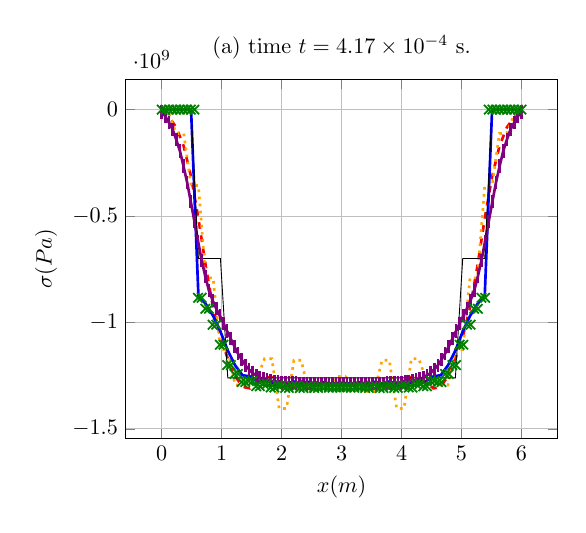
\begin{tikzpicture}[scale=0.8]
\begin{axis}[xlabel=$x (m)$,ylabel=$\sigma (Pa)$,ymajorgrids=true,xmajorgrids=true,legend pos=outer north east,title={(a) time $t = 4.17\times 10^{-4} $ s.}]
\addplot[Red,very thick,mark=none,dashed,mark size=3pt] coordinates {(0.0,-9466083.71137175) (0.12244897959183673,-35514206.734367736) (0.24489795918367346,-84113776.24908806) (0.36734693877551017,-172446629.58542818) (0.4897959183673469,-314805947.20807856) (0.6122448979591837,-511629446.98755276) (0.7346938775510203,-736313113.7069598) (0.8571428571428571,-931144828.2647986) (0.9795918367346939,-1068053644.3292406) (1.1020408163265305,-1170764300.0847378) (1.2244897959183674,-1252110103.6024575) (1.346938775510204,-1302676056.5462253) (1.4693877551020407,-1310165737.6186237) (1.5918367346938775,-1279757193.7171304) (1.7142857142857142,-1256553263.265204) (1.836734693877551,-1258006223.1072822) (1.9591836734693877,-1294050482.3234062) (2.0816326530612246,-1300642620.5987113) (2.204081632653061,-1307227334.5769467) (2.326530612244898,-1275303748.496001) (2.4489795918367347,-1289208797.7645764) (2.571428571428571,-1280826893.2226717) (2.693877551020408,-1303157436.709725) (2.816326530612245,-1289006021.9435475) (2.9387755102040813,-1289002398.658552) (3.061224489795918,-1289002460.452313) (3.183673469387755,-1289006071.890395) (3.306122448979592,-1303157225.279095) (3.4285714285714284,-1280827082.3206232) (3.5510204081632653,-1289208893.7221813) (3.673469387755102,-1275303766.5179212) (3.7959183673469385,-1307227387.3540978) (3.9183673469387754,-1300642664.183363) (4.040816326530612,-1294050357.0073159) (4.163265306122449,-1258006259.974342) (4.285714285714286,-1256553191.759347) (4.408163265306122,-1279757267.3487592) (4.530612244897959,-1310165771.052653) (4.653061224489796,-1302676007.627941) (4.775510204081632,-1252110079.6983936) (4.8979591836734695,-1170764547.776224) (5.020408163265306,-1068053501.3343573) (5.142857142857142,-931144730.4547592) (5.26530612244898,-736313057.6797745) (5.387755102040816,-511629430.76423925) (5.5102040816326525,-314805938.17461526) (5.63265306122449,-172446625.3783345) (5.755102040816326,-84113774.55431706) (5.877551020408163,-35514206.14830053) (6.0,-9466083.577332078) };
\addplot[Orange,very thick,mark=none,dotted,mark size=3pt] coordinates {(0.0,-21775616.685123403) (0.12244897959183673,-21775616.72164698) (0.24489795918367346,-112154769.91343763) (0.36734693877551017,-112154770.19419384) (0.4897959183673469,-357061973.86971843) (0.6122448979591837,-357061975.87384665) (0.7346938775510203,-790799603.3382715) (0.8571428571428571,-790799622.7090364) (0.9795918367346939,-1127863861.8971207) (1.1020408163265305,-1127863910.7156112) (1.2244897959183674,-1294097542.9943345) (1.346938775510204,-1294097833.9624486) (1.4693877551020407,-1264908473.5999227) (1.5918367346938775,-1264908907.9452155) (1.7142857142857142,-1170899419.842339) (1.836734693877551,-1170898869.1188018) (1.9591836734693877,-1404729307.196373) (2.0816326530612246,-1404729023.510617) (2.204081632653061,-1178030994.2246718) (2.326530612244898,-1178032103.900689) (2.4489795918367347,-1325532527.4682536) (2.571428571428571,-1325532662.4079945) (2.693877551020408,-1286992617.5223172) (2.816326530612245,-1286992228.933896) (2.9387755102040813,-1254505712.3434386) (3.061224489795918,-1254505904.1655023) (3.183673469387755,-1286992713.028294) (3.306122448979592,-1286993281.7005486) (3.4285714285714284,-1325532286.4512568) (3.5510204081632653,-1325532447.008532) (3.673469387755102,-1178031216.3396027) (3.7959183673469385,-1178031165.6288564) (3.9183673469387754,-1404729070.936975) (4.040816326530612,-1404729206.2986672) (4.163265306122449,-1170899488.2777543) (4.285714285714286,-1170899253.556783) (4.408163265306122,-1264908724.8211215) (4.530612244897959,-1264908806.5057957) (4.653061224489796,-1294097602.037558) (4.775510204081632,-1294097585.2606838) (4.8979591836734695,-1127863890.5307767) (5.020408163265306,-1127863857.5211554) (5.142857142857142,-790799615.9051313) (5.26530612244898,-790799601.5180427) (5.387755102040816,-357061976.4955751) (5.5102040816326525,-357061973.8588882) (5.63265306122449,-112154770.18131427) (5.755102040816326,-112154769.96143283) (5.877551020408163,-21775616.70163) (6.0,-21775616.698375184) };
\addplot[Blue,very thick,mark=none,solid,mark size=3pt] coordinates {(0.0,-6.648826343127885e-07) (0.12244897959183673,4.986619757345916e-07) (0.24489795918367346,-6.648826343127894e-07) (0.36734693877551017,6.648826343127889e-07) (0.4897959183673469,-3.324413171563951e-07) (0.6122448979591837,-874162257.8546059) (0.7346938775510203,-913424760.9782704) (0.8571428571428571,-969365384.6175718) (0.9795918367346939,-1042970790.4967976) (1.1020408163265305,-1132583339.8680727) (1.2244897959183674,-1201739241.5745146) (1.346938775510204,-1248614593.9146428) (1.4693877551020407,-1253812053.171889) (1.5918367346938775,-1277494278.936118) (1.7142857142857142,-1268975112.888906) (1.836734693877551,-1285312313.5954506) (1.9591836734693877,-1275249588.3375967) (2.0816326530612246,-1288549436.3162062) (2.204081632653061,-1278115488.7494104) (2.326530612244898,-1289609709.5365772) (2.4489795918367347,-1280020503.890194) (2.571428571428571,-1288883802.6033092) (2.693877551020408,-1282041862.894144) (2.816326530612245,-1286896451.527247) (2.9387755102040813,-1284697650.7072186) (3.061224489795918,-1284697650.7072196) (3.183673469387755,-1286896451.5272474) (3.306122448979592,-1282041862.8941436) (3.4285714285714284,-1288883802.6033094) (3.5510204081632653,-1280020503.890194) (3.673469387755102,-1289609709.5365787) (3.7959183673469385,-1278115488.74941) (3.9183673469387754,-1288549436.3162065) (4.040816326530612,-1275249588.337598) (4.163265306122449,-1285312313.5954502) (4.285714285714286,-1268975112.8889062) (4.408163265306122,-1277494278.9361184) (4.530612244897959,-1253812053.1718888) (4.653061224489796,-1248614593.914643) (4.775510204081632,-1201739241.5745142) (4.8979591836734695,-1132583339.8680727) (5.020408163265306,-1042970790.496798) (5.142857142857142,-969365384.6175721) (5.26530612244898,-913424760.9782704) (5.387755102040816,-874162257.8546067) (5.5102040816326525,6.648826343127891e-07) (5.63265306122449,-8.311032928909869e-07) (5.755102040816326,6.64882634312789e-07) (5.877551020408163,-4.986619757345927e-07) (6.0,6.648826343127891e-07) };
\addplot[Purple,very thick,mark=|,solid,mark size=3pt] coordinates {(0.0,-11522502.92600226) (0.06060606060606061,-31725620.091397233) (0.12121212121212122,-61304874.4765079) (0.18181818181818182,-93259931.32451278) (0.24242424242424243,-140838495.245558) (0.30303030303030304,-193913468.55103528) (0.36363636363636365,-265213878.38892987) (0.42424242424242425,-342130694.52595234) (0.48484848484848486,-432453677.3208593) (0.5454545454545454,-525041147.1169883) (0.6060606060606061,-618338331.152021) (0.6666666666666667,-708388503.4017504) (0.7272727272727273,-784021969.6614887) (0.7878787878787878,-850474949.5391626) (0.8484848484848485,-896076004.6724114) (0.9090909090909092,-935262643.3934776) (0.9696969696969697,-969337341.7916008) (1.0303030303030303,-1004304635.4591644) (1.0909090909090908,-1040567603.2284905) (1.1515151515151516,-1077307888.8979723) (1.2121212121212122,-1112635201.8637893) (1.2727272727272727,-1146677662.6062891) (1.3333333333333335,-1175184951.6380641) (1.393939393939394,-1201590500.124662) (1.4545454545454546,-1220740340.2067573) (1.5151515151515151,-1238089436.820448) (1.5757575757575757,-1249284876.1027403) (1.6363636363636365,-1259440830.6822593) (1.696969696969697,-1265589775.602502) (1.7575757575757576,-1271283785.6788774) (1.8181818181818183,-1274687789.8815384) (1.878787878787879,-1277922433.571672) (1.9393939393939394,-1279879339.775472) (2.0,-1281783669.6916373) (2.0606060606060606,-1282949267.7273479) (2.121212121212121,-1284109224.9776726) (2.1818181818181817,-1284819623.1742642) (2.2424242424242427,-1285544784.5476487) (2.303030303030303,-1285981972.386752) (2.3636363636363638,-1286442996.2191055) (2.4242424242424243,-1286710383.2766345) (2.484848484848485,-1287006241.599304) (2.5454545454545454,-1287165476.0382879) (2.606060606060606,-1287356422.5321994) (2.666666666666667,-1287445575.37196) (2.7272727272727275,-1287570603.4105794) (2.787878787878788,-1287613773.5740457) (2.8484848484848486,-1287701397.1398175) (2.909090909090909,-1287711163.0639696) (2.9696969696969697,-1287803837.1394258) (3.0303030303030303,-1287803837.1394258) (3.090909090909091,-1287711163.0639691) (3.1515151515151514,-1287701397.1398172) (3.2121212121212124,-1287613773.5740457) (3.272727272727273,-1287570603.4105797) (3.3333333333333335,-1287445575.37196) (3.393939393939394,-1287356422.5321996) (3.4545454545454546,-1287165476.038288) (3.515151515151515,-1287006241.5993047) (3.5757575757575757,-1286710383.276635) (3.6363636363636367,-1286442996.2191057) (3.6969696969696972,-1285981972.386752) (3.757575757575758,-1285544784.547649) (3.8181818181818183,-1284819623.1742642) (3.878787878787879,-1284109224.977673) (3.9393939393939394,-1282949267.7273483) (4.0,-1281783669.6916378) (4.0606060606060606,-1279879339.7754729) (4.121212121212121,-1277922433.571673) (4.181818181818182,-1274687789.881539) (4.242424242424242,-1271283785.678878) (4.303030303030303,-1265589775.602503) (4.363636363636363,-1259440830.6822598) (4.424242424242425,-1249284876.1027408) (4.484848484848485,-1238089436.8204484) (4.545454545454546,-1220740340.206758) (4.606060606060606,-1201590500.124663) (4.666666666666667,-1175184951.6380656) (4.7272727272727275,-1146677662.60629) (4.787878787878788,-1112635201.8637903) (4.848484848484849,-1077307888.8979728) (4.909090909090909,-1040567603.2284908) (4.96969696969697,-1004304635.459165) (5.03030303030303,-969337341.7916014) (5.090909090909091,-935262643.3934779) (5.151515151515151,-896076004.6724123) (5.212121212121212,-850474949.5391635) (5.2727272727272725,-784021969.6614897) (5.333333333333334,-708388503.401751) (5.3939393939393945,-618338331.1520219) (5.454545454545455,-525041147.11698914) (5.515151515151516,-432453677.3208602) (5.575757575757576,-342130694.5259528) (5.636363636363637,-265213878.3889301) (5.696969696969697,-193913468.55103546) (5.757575757575758,-140838495.24555832) (5.818181818181818,-93259931.3245125) (5.878787878787879,-61304874.4765082) (5.9393939393939394,-31725620.091397557) (6.0,-11522502.926002609) };
\addplot[Green,thick,mark=x,only marks,mark size=3pt] coordinates {(0.0,-2.0877147917780336e-07) (0.06060606060606061,-1.23669837978591e-07) (0.12121212121212122,1.0131895444177197e-06) (0.18181818181818182,9.814583585206487e-07) (0.24242424242424243,-5.619879278457838e-07) (0.30303030303030304,-7.677773407797948e-07) (0.36363636363636365,4.815476698956227e-07) (0.42424242424242425,1.8333496441716677e-07) (0.48484848484848486,1.0440135561077701e-07) (0.5454545454545454,2.2803996154561766e-07) (0.6060606060606061,-884550714.70502) (0.6666666666666667,-884550714.7050202) (0.7272727272727273,-936122014.0999393) (0.7878787878787878,-936122014.0999395) (0.8484848484848485,-1010904183.587626) (0.9090909090909092,-1010904183.5876261) (0.9696969696969697,-1105134845.294078) (1.0303030303030303,-1105134845.294077) (1.0909090909090908,-1200693543.9954407) (1.1515151515151516,-1200693543.9954407) (1.2121212121212122,-1242600895.2828481) (1.2727272727272727,-1242600895.2828481) (1.3333333333333335,-1280378553.9593801) (1.393939393939394,-1280378553.9593809) (1.4545454545454546,-1275721452.5659273) (1.5151515151515151,-1275721452.5659602) (1.5757575757575757,-1300299286.3908393) (1.6363636363636365,-1300299286.3908374) (1.696969696969697,-1289272425.5395763) (1.7575757575757576,-1289272425.5395694) (1.8181818181818183,-1306127301.5683103) (1.878787878787879,-1306127301.5683022) (1.9393939393939394,-1296028797.1903882) (2.0,-1296028797.1903853) (2.0606060606060606,-1308123608.354041) (2.121212121212121,-1308123608.3541112) (2.1818181818181817,-1299597735.2461388) (2.2424242424242427,-1299597735.246238) (2.303030303030303,-1308620980.1784377) (2.3636363636363638,-1308620980.1784313) (2.4242424242424243,-1301801281.3713925) (2.484848484848485,-1301801281.3713658) (2.5454545454545454,-1308121765.4283872) (2.606060606060606,-1308121765.4283755) (2.666666666666667,-1303587683.0677166) (2.7272727272727275,-1303587683.0677037) (2.787878787878788,-1306911469.4399674) (2.8484848484848486,-1306911469.4400563) (2.909090909090909,-1305310135.1663263) (2.9696969696969697,-1305310135.1662202) (3.0303030303030303,-1305310135.1663122) (3.090909090909091,-1305310135.1663315) (3.1515151515151514,-1306911469.4400697) (3.2121212121212124,-1306911469.4400973) (3.272727272727273,-1303587683.067521) (3.3333333333333335,-1303587683.0675333) (3.393939393939394,-1308121765.428341) (3.4545454545454546,-1308121765.4283326) (3.515151515151515,-1301801281.3712707) (3.5757575757575757,-1301801281.3712776) (3.6363636363636367,-1308620980.1785724) (3.6969696969696972,-1308620980.1785636) (3.757575757575758,-1299597735.2460728) (3.8181818181818183,-1299597735.2461448) (3.878787878787879,-1308123608.3541088) (3.9393939393939394,-1308123608.3540418) (4.0,-1296028797.1904147) (4.0606060606060606,-1296028797.190405) (4.121212121212121,-1306127301.5683162) (4.181818181818182,-1306127301.5683157) (4.242424242424242,-1289272425.5394864) (4.303030303030303,-1289272425.5394852) (4.363636363636363,-1300299286.390773) (4.424242424242425,-1300299286.3907716) (4.484848484848485,-1275721452.565949) (4.545454545454546,-1275721452.565983) (4.606060606060606,-1280378553.9593606) (4.666666666666667,-1280378553.9593616) (4.7272727272727275,-1242600895.2828217) (4.787878787878788,-1242600895.2828217) (4.848484848484849,-1200693543.9954677) (4.909090909090909,-1200693543.9954684) (4.96969696969697,-1105134845.294094) (5.03030303030303,-1105134845.2940938) (5.090909090909091,-1010904183.5876323) (5.151515151515151,-1010904183.5876321) (5.212121212121212,-936122014.0999426) (5.2727272727272725,-936122014.0999423) (5.333333333333334,-884550714.7050228) (5.3939393939393945,-884550714.7050234) (5.454545454545455,6.698192810303248e-07) (5.515151515151516,6.599459875952535e-07) (5.575757575757576,-9.369788715662316e-07) (5.636363636363637,-1.0576690313721361e-06) (5.696969696969697,1.675441116120912e-06) (5.757575757575758,1.6489720554430353e-06) (5.818181818181818,-1.0608989471845062e-06) (5.878787878787879,-9.337489557538617e-07) (5.9393939393939394,1.4751713795395358e-06) (6.0,1.5168004748680168e-06) };
\addplot[black,thin,mark=none,solid,mark size=3pt] coordinates {(0.0,-0.0) (0.12244897959183673,-0.0) (0.24489795918367346,-0.0) (0.36734693877551017,-0.0) (0.4897959183673469,-0.0) (0.6122448979591837,-700000000.0) (0.7346938775510203,-700000000.0) (0.8571428571428571,-700000000.0) (0.9795918367346939,-700000000.0) (1.1020408163265305,-1261004576.260559) (1.2244897959183674,-1261004576.260559) (1.346938775510204,-1261004576.260559) (1.4693877551020407,-1261004576.260559) (1.5918367346938775,-1261004576.260559) (1.7142857142857142,-1261004576.260559) (1.836734693877551,-1261004576.260559) (1.9591836734693877,-1261004576.260559) (2.0816326530612246,-1261004576.260559) (2.204081632653061,-1261004576.260559) (2.326530612244898,-1261004576.260559) (2.4489795918367347,-1261004576.260559) (2.571428571428571,-1261004576.260559) (2.693877551020408,-1261004576.260559) (2.816326530612245,-1261004576.260559) (2.9387755102040813,-1261004576.260559) (3.061224489795918,-1261004576.260559) (3.183673469387755,-1261004576.260559) (3.306122448979592,-1261004576.260559) (3.4285714285714284,-1261004576.260559) (3.5510204081632653,-1261004576.260559) (3.673469387755102,-1261004576.260559) (3.7959183673469385,-1261004576.260559) (3.9183673469387754,-1261004576.260559) (4.040816326530612,-1261004576.260559) (4.163265306122449,-1261004576.260559) (4.285714285714286,-1261004576.260559) (4.408163265306122,-1261004576.260559) (4.530612244897959,-1261004576.260559) (4.653061224489796,-1261004576.260559) (4.775510204081632,-1261004576.260559) (4.8979591836734695,-1261004576.260559) (5.020408163265306,-700000000.0) (5.142857142857142,-700000000.0) (5.26530612244898,-700000000.0) (5.387755102040816,-700000000.0) (5.5102040816326525,-0.0) (5.63265306122449,-0.0) (5.755102040816326,-0.0) (5.877551020408163,-0.0) (6.0,-0.0) };
%\legend{usl 1ppc,usf 1ppc,dgmpm 1ppc,dgmpm 2ppc,dgmpm 2ppc (RK2 + strang),plastic solution}
\end{axis}
\end{tikzpicture}
%%% Local Variables:
%%% mode: latex
%%% TeX-master: "../../mainManuscript"
%%% End:
}
  % {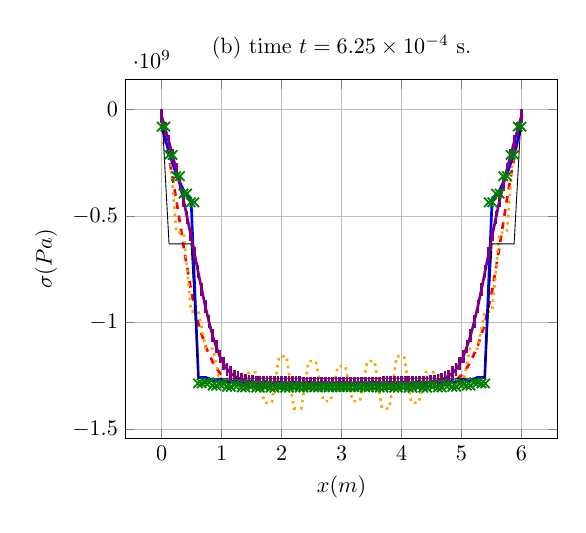
\begin{tikzpicture}[scale=0.8]
\begin{axis}[xlabel=$x (m)$,ylabel=$\sigma (Pa)$,ymajorgrids=true,xmajorgrids=true,legend pos=outer north east,title={(b) time $t = 6.25\times 10^{-4} $ s.}]
\addplot[Red,very thick,mark=none,dashed,mark size=3pt] coordinates {(0.0,-68320403.62221353) (0.12244897959183673,-225789676.02918974) (0.24489795918367346,-424791619.04833) (0.36734693877551017,-646380796.7713014) (0.4897959183673469,-849944016.2028724) (0.6122448979591837,-1006146061.0400205) (0.7346938775510203,-1114292580.0561018) (0.8571428571428571,-1188728982.2247245) (0.9795918367346939,-1241700251.4602263) (1.1020408163265305,-1273020972.5655205) (1.2244897959183674,-1284949093.1656094) (1.346938775510204,-1280762376.3082383) (1.4693877551020407,-1280131918.3035223) (1.5918367346938775,-1279490959.2062156) (1.7142857142857142,-1290763235.7380192) (1.836734693877551,-1286886471.7575386) (1.9591836734693877,-1293425757.5226574) (2.0816326530612246,-1281287553.8251324) (2.204081632653061,-1292409766.4422443) (2.326530612244898,-1282629752.438702) (2.4489795918367347,-1294945401.113779) (2.571428571428571,-1283794612.9732673) (2.693877551020408,-1291887694.9803798) (2.816326530612245,-1285785861.1559482) (2.9387755102040813,-1289860908.4664276) (3.061224489795918,-1289860960.9809775) (3.183673469387755,-1285785837.4934893) (3.306122448979592,-1291887487.9744287) (3.4285714285714284,-1283794664.8462174) (3.5510204081632653,-1294945447.7560375) (3.673469387755102,-1282629760.5221589) (3.7959183673469385,-1292409767.8294322) (3.9183673469387754,-1281287565.3495717) (4.040816326530612,-1293425764.3679597) (4.163265306122449,-1286886489.0287468) (4.285714285714286,-1290763226.34359) (4.408163265306122,-1279490965.7329388) (4.530612244897959,-1280131956.1996849) (4.653061224489796,-1280762451.4159694) (4.775510204081632,-1284949184.1714568) (4.8979591836734695,-1273020948.2916741) (5.020408163265306,-1241700137.1761186) (5.142857142857142,-1188728796.523432) (5.26530612244898,-1114292407.0488575) (5.387755102040816,-1006146274.5465661) (5.5102040816326525,-849944214.1880462) (5.63265306122449,-646381051.5707061) (5.755102040816326,-424791730.9041514) (5.877551020408163,-225789800.60525674) (6.0,-68320454.65089296) };
\addplot[Orange,very thick,mark=none,dotted,mark size=3pt] coordinates {(0.0,-156995048.72300234) (0.12244897959183673,-156995364.03184575) (0.24489795918367346,-578361553.8773596) (0.36734693877551017,-578361776.9652294) (0.4897959183673469,-947878572.789029) (0.6122448979591837,-947878629.0454134) (0.7346938775510203,-1122155365.9445817) (0.8571428571428571,-1122155222.890123) (0.9795918367346939,-1291825792.2012048) (1.1020408163265305,-1291825773.3810687) (1.2244897959183674,-1251635171.0476031) (1.346938775510204,-1251635100.0260744) (1.4693877551020407,-1232474111.1713145) (1.5918367346938775,-1232473886.0470812) (1.7142857142857142,-1376816804.9626572) (1.836734693877551,-1376817081.1171806) (1.9591836734693877,-1157922444.4640186) (2.0816326530612246,-1157922510.7665095) (2.204081632653061,-1403184236.5989518) (2.326530612244898,-1403184536.0603929) (2.4489795918367347,-1180859401.2507882) (2.571428571428571,-1180859508.133819) (2.693877551020408,-1368793239.5548983) (2.816326530612245,-1368793451.4344292) (2.9387755102040813,-1203835945.0107105) (3.061224489795918,-1203835622.7844667) (3.183673469387755,-1368793306.427742) (3.306122448979592,-1368793478.6580884) (3.4285714285714284,-1180859183.8880649) (3.5510204081632653,-1180859290.5038683) (3.673469387755102,-1403184136.6867287) (3.7959183673469385,-1403183761.77251) (3.9183673469387754,-1157922482.3658946) (4.040816326530612,-1157922352.2307622) (4.163265306122449,-1376817001.1907525) (4.285714285714286,-1376817315.2298005) (4.408163265306122,-1232474572.3256762) (4.530612244897959,-1232474451.4669452) (4.653061224489796,-1251634884.2142015) (4.775510204081632,-1251635269.3170545) (4.8979591836734695,-1291825665.5679488) (5.020408163265306,-1291825906.6643884) (5.142857142857142,-1122155225.5621386) (5.26530612244898,-1122155914.2048798) (5.387755102040816,-947878625.770502) (5.5102040816326525,-947877795.5933025) (5.63265306122449,-578361684.1093763) (5.755102040816326,-578362214.7513508) (5.877551020408163,-156995223.63768175) (6.0,-156995328.8817121) };
\addplot[Blue,very thick,mark=none,solid,mark size=3pt] coordinates {(0.0,-78094246.59211227) (0.12244897959183673,-202047177.96964124) (0.24489795918367346,-306454110.06972677) (0.36734693877551017,-380145390.26078814) (0.4897959183673469,-423404735.09272164) (0.6122448979591837,-1257853636.3109157) (0.7346938775510203,-1257085473.8466249) (0.8571428571428571,-1273738336.1650534) (0.9795918367346939,-1266172602.6079874) (1.1020408163265305,-1281249763.7189615) (1.2244897959183674,-1270901976.3756995) (1.346938775510204,-1284583664.611882) (1.4693877551020407,-1273997234.574172) (1.5918367346938775,-1285577300.0190902) (1.7142857142857142,-1276400493.5524273) (1.836734693877551,-1285417293.975184) (1.9591836734693877,-1278339664.6925926) (2.0816326530612246,-1284852686.1476386) (2.204081632653061,-1279850028.976812) (2.326530612244898,-1284238970.623943) (2.4489795918367347,-1280987011.9763784) (2.571428571428571,-1283670980.1448214) (2.693877551020408,-1281846768.3113825) (2.816326530612245,-1283114948.4817128) (2.9387755102040813,-1282695202.1981924) (3.061224489795918,-1282695202.1981914) (3.183673469387755,-1283114948.4817138) (3.306122448979592,-1281846768.3113823) (3.4285714285714284,-1283670980.1448233) (3.5510204081632653,-1280987011.9763772) (3.673469387755102,-1284238970.6239436) (3.7959183673469385,-1279850028.9768124) (3.9183673469387754,-1284852686.147639) (4.040816326530612,-1278339664.6925926) (4.163265306122449,-1285417293.9751842) (4.285714285714286,-1276400493.5524268) (4.408163265306122,-1285577300.0190902) (4.530612244897959,-1273997234.5741723) (4.653061224489796,-1284583664.6118824) (4.775510204081632,-1270901976.3757002) (4.8979591836734695,-1281249763.718962) (5.020408163265306,-1266172602.6079872) (5.142857142857142,-1273738336.1650534) (5.26530612244898,-1257085473.8466249) (5.387755102040816,-1257853636.3109152) (5.5102040816326525,-423404735.092723) (5.63265306122449,-380145390.2607865) (5.755102040816326,-306454110.0697275) (5.877551020408163,-202047177.96964) (6.0,-78094246.59211358) };
\addplot[Purple,very thick,mark=|,solid,mark size=3pt] coordinates {(0.0,-29927303.866736423) (0.06060606060606061,-91056397.63368599) (0.12121212121212122,-151613704.523153) (0.18181818181818182,-216112605.28132087) (0.24242424242424243,-280335641.2622369) (0.30303030303030304,-352344393.75337386) (0.36363636363636365,-424489613.7233627) (0.42424242424242425,-505847292.410384) (0.48484848484848486,-586999789.9597377) (0.5454545454545454,-673998041.6926832) (0.6060606060606061,-759351839.9800754) (0.6666666666666667,-843513643.4035325) (0.7272727272727273,-923946644.5385387) (0.7878787878787878,-995414783.6619084) (0.8484848484848485,-1061232446.5295665) (0.9090909090909092,-1113218962.1696506) (0.9696969696969697,-1159051731.4367843) (1.0303030303030303,-1191404581.2317898) (1.0909090909090908,-1218844186.0222213) (1.1515151515151516,-1236684855.8963497) (1.2121212121212122,-1251383919.797765) (1.2727272727272727,-1260493728.1975224) (1.3333333333333335,-1267812955.7854612) (1.393939393939394,-1272272932.5908973) (1.4545454545454546,-1275765921.540089) (1.5151515151515151,-1277936320.3680944) (1.5757575757575757,-1279592582.5775201) (1.6363636363636365,-1280693510.9832897) (1.696969696969697,-1281513981.0637147) (1.7575757575757576,-1282125151.9012914) (1.8181818181818183,-1282572071.178818) (1.878787878787879,-1282950867.4850798) (1.9393939393939394,-1283223494.4286144) (2.0,-1283480133.76503) (2.0606060606060606,-1283661506.7126255) (2.121212121212121,-1283844490.520339) (2.1818181818181817,-1283970476.588324) (2.2424242424242427,-1284103730.0809987) (2.303030303030303,-1284191946.2274148) (2.3636363636363638,-1284289437.5825508) (2.4242424242424243,-1284350224.7858446) (2.484848484848485,-1284421413.7540164) (2.5454545454545454,-1284461770.7762535) (2.606060606060606,-1284513746.332839) (2.666666666666667,-1284538764.3494127) (2.7272727272727275,-1284577367.2906) (2.787878787878788,-1284590745.1308227) (2.8484848484848486,-1284621851.9102542) (2.909090909090909,-1284624878.9151099) (2.9696969696969697,-1284663796.6518083) (3.0303030303030303,-1284663796.6518083) (3.090909090909091,-1284624878.9151099) (3.1515151515151514,-1284621851.9102545) (3.2121212121212124,-1284590745.1308224) (3.272727272727273,-1284577367.2906) (3.3333333333333335,-1284538764.3494127) (3.393939393939394,-1284513746.332839) (3.4545454545454546,-1284461770.7762532) (3.515151515151515,-1284421413.7540162) (3.5757575757575757,-1284350224.7858446) (3.6363636363636367,-1284289437.582551) (3.6969696969696972,-1284191946.227415) (3.757575757575758,-1284103730.0809991) (3.8181818181818183,-1283970476.5883245) (3.878787878787879,-1283844490.5203397) (3.9393939393939394,-1283661506.712626) (4.0,-1283480133.7650306) (4.0606060606060606,-1283223494.4286153) (4.121212121212121,-1282950867.4850807) (4.181818181818182,-1282572071.1788187) (4.242424242424242,-1282125151.901292) (4.303030303030303,-1281513981.0637155) (4.363636363636363,-1280693510.9832904) (4.424242424242425,-1279592582.577521) (4.484848484848485,-1277936320.3680952) (4.545454545454546,-1275765921.5400894) (4.606060606060606,-1272272932.5908978) (4.666666666666667,-1267812955.785462) (4.7272727272727275,-1260493728.1975229) (4.787878787878788,-1251383919.797766) (4.848484848484849,-1236684855.8963506) (4.909090909090909,-1218844186.0222228) (4.96969696969697,-1191404581.231791) (5.03030303030303,-1159051731.4367847) (5.090909090909091,-1113218962.169651) (5.151515151515151,-1061232446.529567) (5.212121212121212,-995414783.6619091) (5.2727272727272725,-923946644.5385387) (5.333333333333334,-843513643.4035326) (5.3939393939393945,-759351839.9800754) (5.454545454545455,-673998041.6926835) (5.515151515151516,-586999789.9597379) (5.575757575757576,-505847292.4103844) (5.636363636363637,-424489613.7233631) (5.696969696969697,-352344393.7533744) (5.757575757575758,-280335641.2622374) (5.818181818181818,-216112605.28132126) (5.878787878787879,-151613704.5231535) (5.9393939393939394,-91056397.63368621) (6.0,-29927303.86673645) };
\addplot[Green,thick,mark=x,only marks,mark size=3pt] coordinates {(0.0,-79916002.67055239) (0.06060606060606061,-79916002.67055224) (0.12121212121212122,-212751355.9722632) (0.18181818181818182,-212751355.97226292) (0.24242424242424243,-312518540.6021343) (0.30303030303030304,-312518540.60213417) (0.36363636363636365,-394252960.7380532) (0.42424242424242425,-394252960.73804915) (0.48484848484848486,-435228881.2798793) (0.5454545454545454,-435228881.27987766) (0.6060606060606061,-1285411981.4217432) (0.6666666666666667,-1285411981.4217405) (0.7272727272727273,-1280711603.3230183) (0.7878787878787878,-1280711603.3230135) (0.8484848484848485,-1295937493.3862524) (0.9090909090909092,-1295937493.3862624) (0.9696969696969697,-1287988489.6130652) (1.0303030303030303,-1287988489.6129992) (1.0909090909090908,-1301349142.6084783) (1.1515151515151516,-1301349142.6085305) (1.2121212121212122,-1292031977.182477) (1.2727272727272727,-1292031977.1824605) (1.3333333333333335,-1304158962.6097703) (1.393939393939394,-1304158962.609774) (1.4545454545454546,-1294615911.7133598) (1.5151515151515151,-1294615911.713364) (1.5757575757575757,-1305409469.234389) (1.6363636363636365,-1305409469.2343793) (1.696969696969697,-1296575097.169732) (1.7575757575757576,-1296575097.1696386) (1.8181818181818183,-1305694934.8057256) (1.878787878787879,-1305694934.8056414) (1.9393939393939394,-1298237888.1883545) (2.0,-1298237888.1883388) (2.0606060606060606,-1305422829.3343308) (2.121212121212121,-1305422829.3343291) (2.1818181818181817,-1299681183.8928425) (2.2424242424242427,-1299681183.8927386) (2.303030303030303,-1304867646.3713446) (2.3636363636363638,-1304867646.3713348) (2.4242424242424243,-1300902385.280055) (2.484848484848485,-1300902385.280057) (2.5454545454545454,-1304201666.8734922) (2.606060606060606,-1304201666.8733885) (2.666666666666667,-1301910986.9763758) (2.7272727272727275,-1301910986.9763756) (2.787878787878788,-1303498906.5357742) (2.8484848484848486,-1303498906.535786) (2.909090909090909,-1302755121.5435212) (2.9696969696969697,-1302755121.5435221) (3.0303030303030303,-1302755121.543637) (3.090909090909091,-1302755121.543634) (3.1515151515151514,-1303498906.5355883) (3.2121212121212124,-1303498906.5355833) (3.272727272727273,-1301910986.97636) (3.3333333333333335,-1301910986.9762814) (3.393939393939394,-1304201666.8734074) (3.4545454545454546,-1304201666.8733807) (3.515151515151515,-1300902385.280354) (3.5757575757575757,-1300902385.2803435) (3.6363636363636367,-1304867646.3712885) (3.6969696969696972,-1304867646.3712816) (3.757575757575758,-1299681183.8926687) (3.8181818181818183,-1299681183.8927484) (3.878787878787879,-1305422829.3345184) (3.9393939393939394,-1305422829.3345306) (4.0,-1298237888.1883025) (4.0606060606060606,-1298237888.1882656) (4.121212121212121,-1305694934.8057399) (4.181818181818182,-1305694934.8057516) (4.242424242424242,-1296575097.1697433) (4.303030303030303,-1296575097.1697195) (4.363636363636363,-1305409469.2346466) (4.424242424242425,-1305409469.2346435) (4.484848484848485,-1294615911.7133439) (4.545454545454546,-1294615911.713418) (4.606060606060606,-1304158962.609734) (4.666666666666667,-1304158962.6097326) (4.7272727272727275,-1292031977.1825411) (4.787878787878788,-1292031977.1825192) (4.848484848484849,-1301349142.6085944) (4.909090909090909,-1301349142.6086338) (4.96969696969697,-1287988489.6129642) (5.03030303030303,-1287988489.6129599) (5.090909090909091,-1295937493.3861973) (5.151515151515151,-1295937493.38624) (5.212121212121212,-1280711603.3229506) (5.2727272727272725,-1280711603.3229578) (5.333333333333334,-1285411981.4217515) (5.3939393939393945,-1285411981.4217482) (5.454545454545455,-435228881.27979714) (5.515151515151516,-435228881.2797981) (5.575757575757576,-394252960.7380172) (5.636363636363637,-394252960.7380113) (5.696969696969697,-312518540.6021377) (5.757575757575758,-312518540.6021374) (5.818181818181818,-212751355.9722441) (5.878787878787879,-212751355.97224396) (5.9393939393939394,-79916002.67054233) (6.0,-79916002.67054217) };
\addplot[black,thin,mark=none,solid,mark size=3pt] coordinates {(0.0,-0.0) (0.12244897959183673,-630502288.1302795) (0.24489795918367346,-630502288.1302795) (0.36734693877551017,-630502288.1302795) (0.4897959183673469,-630502288.1302795) (0.6122448979591837,-1261004576.260559) (0.7346938775510203,-1261004576.260559) (0.8571428571428571,-1261004576.260559) (0.9795918367346939,-1261004576.260559) (1.1020408163265305,-1261004576.260559) (1.2244897959183674,-1261004576.260559) (1.346938775510204,-1261004576.260559) (1.4693877551020407,-1261004576.260559) (1.5918367346938775,-1261004576.260559) (1.7142857142857142,-1261004576.260559) (1.836734693877551,-1261004576.260559) (1.9591836734693877,-1261004576.260559) (2.0816326530612246,-1261004576.260559) (2.204081632653061,-1261004576.260559) (2.326530612244898,-1261004576.260559) (2.4489795918367347,-1261004576.260559) (2.571428571428571,-1261004576.260559) (2.693877551020408,-1261004576.260559) (2.816326530612245,-1261004576.260559) (2.9387755102040813,-1261004576.260559) (3.061224489795918,-1261004576.260559) (3.183673469387755,-1261004576.260559) (3.306122448979592,-1261004576.260559) (3.4285714285714284,-1261004576.260559) (3.5510204081632653,-1261004576.260559) (3.673469387755102,-1261004576.260559) (3.7959183673469385,-1261004576.260559) (3.9183673469387754,-1261004576.260559) (4.040816326530612,-1261004576.260559) (4.163265306122449,-1261004576.260559) (4.285714285714286,-1261004576.260559) (4.408163265306122,-1261004576.260559) (4.530612244897959,-1261004576.260559) (4.653061224489796,-1261004576.260559) (4.775510204081632,-1261004576.260559) (4.8979591836734695,-1261004576.260559) (5.020408163265306,-1261004576.260559) (5.142857142857142,-1261004576.260559) (5.26530612244898,-1261004576.260559) (5.387755102040816,-1261004576.260559) (5.5102040816326525,-630502288.1302795) (5.63265306122449,-630502288.1302795) (5.755102040816326,-630502288.1302795) (5.877551020408163,-630502288.1302795) (6.0,-0.0) };
%\legend{usl 1ppc,usf 1ppc,dgmpm 1ppc,dgmpm 2ppc,dgmpm 2ppc (RK2 + strang),plastic solution}
\end{axis}
\end{tikzpicture}
%%% Local Variables:
%%% mode: latex
%%% TeX-master: "../../mainManuscript"
%%% End:
}
  % {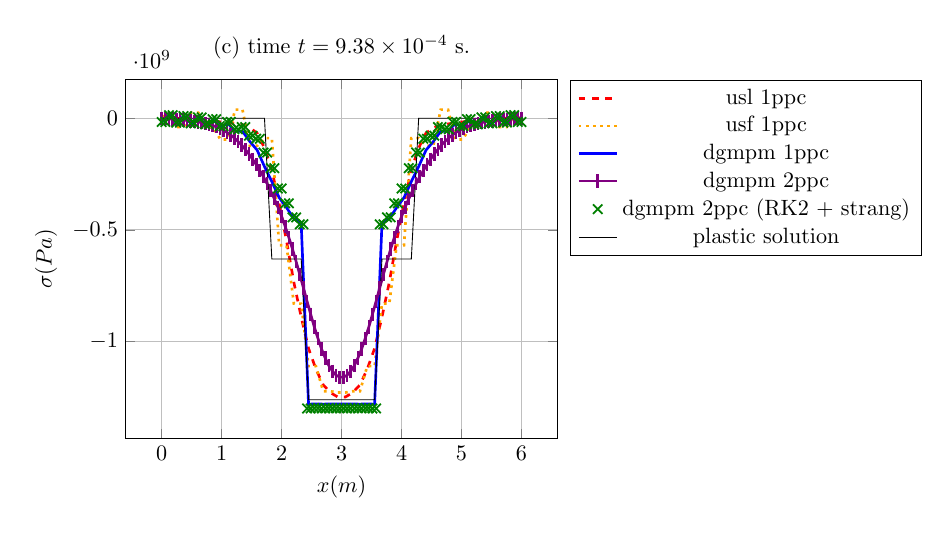
\begin{tikzpicture}[scale=0.8]
\begin{axis}[xlabel=$x (m)$,ylabel=$\sigma (Pa)$,ymajorgrids=true,xmajorgrids=true,legend pos=outer north east,title={(c) time $t = 9.38\times 10^{-4} $ s.}]
\addplot[Red,very thick,mark=none,dashed,mark size=3pt] coordinates {(0.0,2179887.8741577687) (0.12244897959183673,4271567.711108255) (0.24489795918367346,966738.2718996657) (0.36734693877551017,-6271723.611613803) (0.4897959183673469,-14030025.543121472) (0.6122448979591837,-17300156.3048836) (0.7346938775510203,-17305066.9959836) (0.8571428571428571,-14566418.551567167) (0.9795918367346939,-16305735.244086802) (1.1020408163265305,-18440246.43842104) (1.2244897959183674,-25972388.96555254) (1.346938775510204,-28555956.198484987) (1.4693877551020407,-43094669.87634274) (1.5918367346938775,-66731576.159464) (1.7142857142857142,-133302673.15943551) (1.836734693877551,-231217066.04087403) (1.9591836734693877,-383807433.4614241) (2.0816326530612246,-549183051.8960142) (2.204081632653061,-735150557.5668448) (2.326530612244898,-890613203.5459447) (2.4489795918367347,-1031087113.7887726) (2.571428571428571,-1123706429.10668) (2.693877551020408,-1194507158.1924114) (2.816326530612245,-1229880900.951359) (2.9387755102040813,-1249229731.1506605) (3.061224489795918,-1249229803.8387284) (3.183673469387755,-1229880902.2439501) (3.306122448979592,-1194507007.9696314) (3.4285714285714284,-1123706429.6820912) (3.5510204081632653,-1031087100.453649) (3.673469387755102,-890613181.8274102) (3.7959183673469385,-735150574.6185814) (3.9183673469387754,-549183123.0526139) (4.040816326530612,-383807527.3296739) (4.163265306122449,-231217177.34179434) (4.285714285714286,-133302750.31143498) (4.408163265306122,-66731611.9840056) (4.530612244897959,-43094655.69694871) (4.653061224489796,-28555893.171867877) (4.775510204081632,-25972299.275931567) (4.8979591836734695,-18440109.135098517) (5.020408163265306,-16305650.867872208) (5.142857142857142,-14566439.8601152) (5.26530612244898,-17305083.8923935) (5.387755102040816,-17300346.919932812) (5.5102040816326525,-14030070.633207008) (5.63265306122449,-6271789.10862004) (5.755102040816326,966856.2919337559) (5.877551020408163,4271661.846636482) (6.0,2179930.654313549) };
\addplot[Orange,very thick,mark=none,dotted,mark size=3pt] coordinates {(0.0,8883152.476342868) (0.12244897959183673,8883358.002238374) (0.24489795918367346,-39614765.19711469) (0.36734693877551017,-39614781.617487594) (0.4897959183673469,24130879.525100976) (0.6122448979591837,24130829.63196762) (0.7346938775510203,-40981273.713695824) (0.8571428571428571,-40980726.61947498) (0.9795918367346939,-95245444.76221448) (1.1020408163265305,-95245719.55893344) (1.2244897959183674,38559738.26329234) (1.346938775510204,38559724.01425779) (1.4693877551020407,-123578328.23144782) (1.5918367346938775,-123578620.59498507) (1.7142857142857142,-89067391.13390172) (1.836734693877551,-89067687.0153715) (1.9591836734693877,-568996208.7327635) (2.0816326530612246,-568996136.0973773) (2.204081632653061,-830835672.4769804) (2.326530612244898,-830836152.4761271) (2.4489795918367347,-1110775491.352927) (2.571428571428571,-1110775490.2064652) (2.693877551020408,-1223264981.9607182) (2.816326530612245,-1223264942.7032547) (2.9387755102040813,-1228957267.7971613) (3.061224489795918,-1228957189.2818208) (3.183673469387755,-1223264630.7040293) (3.306122448979592,-1223264842.4695811) (3.4285714285714284,-1110775448.9306216) (3.5510204081632653,-1110775936.5413404) (3.673469387755102,-830835758.9049939) (3.7959183673469385,-830835610.4351878) (3.9183673469387754,-568996303.5281599) (4.040816326530612,-568996287.8557086) (4.163265306122449,-89067587.66263753) (4.285714285714286,-89067845.72452801) (4.408163265306122,-123578268.096769) (4.530612244897959,-123578358.14286369) (4.653061224489796,38559843.5755333) (4.775510204081632,38559828.238871574) (4.8979591836734695,-95245164.13589382) (5.020408163265306,-95245758.53559154) (5.142857142857142,-40981325.88530624) (5.26530612244898,-40980952.94831386) (5.387755102040816,24130912.477825537) (5.5102040816326525,24131492.332650885) (5.63265306122449,-39614327.50948672) (5.755102040816326,-39614529.485087976) (5.877551020408163,8883033.068865106) (6.0,8882866.208991345) };
\addplot[Blue,very thick,mark=none,solid,mark size=3pt] coordinates {(0.0,-17128300.102667417) (0.12244897959183673,13752835.432253828) (0.24489795918367346,-20542070.36579649) (0.36734693877551017,9627575.944852384) (0.4897959183673469,-24583114.49486078) (0.6122448979591837,3553087.8993602726) (0.7346938775510203,-30196416.494030617) (0.8571428571428571,-6254279.5006018765) (0.9795918367346939,-39643433.03070669) (1.1020408163265305,-23398742.14579887) (1.2244897959183674,-58622349.405956574) (1.346938775510204,-58612611.005193084) (1.4693877551020407,-104358757.95436558) (1.5918367346938775,-142747990.62676075) (1.7142857142857142,-216604223.34056965) (1.836734693877551,-284014503.7465758) (1.9591836734693877,-355763297.3031307) (2.0816326530612246,-400412643.93499076) (2.204081632653061,-450041758.38666886) (2.326530612244898,-471943820.1052512) (2.4489795918367347,-1281104809.5651186) (2.571428571428571,-1279794858.2655103) (2.693877551020408,-1280800959.7472942) (2.816326530612245,-1280157396.7060692) (2.9387755102040813,-1280585488.3021743) (3.061224489795918,-1280585488.302175) (3.183673469387755,-1280157396.7060692) (3.306122448979592,-1280800959.7472951) (3.4285714285714284,-1279794858.2655094) (3.5510204081632653,-1281104809.5651186) (3.673469387755102,-471943820.10525143) (3.7959183673469385,-450041758.3866677) (3.9183673469387754,-400412643.9349916) (4.040816326530612,-355763297.3031296) (4.163265306122449,-284014503.74657553) (4.285714285714286,-216604223.34056863) (4.408163265306122,-142747990.62676063) (4.530612244897959,-104358757.95436497) (4.653061224489796,-58612611.00519418) (4.775510204081632,-58622349.40595588) (4.8979591836734695,-23398742.145799696) (5.020408163265306,-39643433.03070569) (5.142857142857142,-6254279.500602099) (5.26530612244898,-30196416.494029872) (5.387755102040816,3553087.899359706) (5.5102040816326525,-24583114.494859148) (5.63265306122449,9627575.944852106) (5.755102040816326,-20542070.365794413) (5.877551020408163,13752835.432252467) (6.0,-17128300.10266669) };
\addplot[Purple,very thick,mark=|,solid,mark size=3pt] coordinates {(0.0,-541585.4569046181) (0.06060606060606061,-1707474.8835564104) (0.12121212121212122,-2830207.55651644) (0.18181818181818182,-4085576.273737057) (0.24242424242424243,-5333599.888376622) (0.30303030303030304,-6783527.424069693) (0.36363636363636365,-8264113.22583064) (0.42424242424242425,-10048634.75441422) (0.48484848484848486,-11910748.32917964) (0.5454545454545454,-14231193.751474395) (0.6060606060606061,-16693688.049955105) (0.6666666666666667,-19846444.732987218) (0.7272727272727273,-23233445.153957445) (0.7878787878787878,-27643962.404877316) (0.8484848484848485,-32417320.089586973) (0.9090909090909092,-38654451.54188632) (0.9696969696969697,-45419294.84551809) (1.0303030303030303,-54159189.00456727) (1.0909090909090908,-63609801.58190335) (1.1515151515151516,-75525254.67750409) (1.2121212121212122,-88312648.84858769) (1.2727272727272727,-103904227.46168624) (1.3333333333333335,-120458077.3316795) (1.393939393939394,-139913393.9011292) (1.4545454545454546,-160326296.83086172) (1.5151515151515151,-183546734.18897414) (1.5757575757575757,-207666482.259661) (1.6363636363636365,-234552749.3577987) (1.696969696969697,-262339698.06796068) (1.7575757575757576,-293232999.53865474) (1.8181818181818183,-325207293.9873926) (1.878787878787879,-361144702.9112083) (1.9393939393939394,-398529242.72082573) (2.0,-440933710.48029673) (2.0606060606060606,-485152835.4909869) (2.121212121212121,-534896828.13938504) (2.1818181818181817,-586502388.8960851) (2.2424242424242427,-642788141.8891436) (2.303030303030303,-700380650.3721517) (2.3636363636363638,-760150889.2209504) (2.4242424242424243,-820009358.6982999) (2.484848484848485,-878356122.5558186) (2.5454545454545454,-935101641.3519866) (2.606060606060606,-986513990.571936) (2.666666666666667,-1034469694.8460171) (2.7272727272727275,-1074217363.83751) (2.787878787878788,-1108703084.7840602) (2.8484848484848486,-1133621193.2437282) (2.909090909090909,-1151583876.8985791) (2.9696969696969697,-1160048656.4594278) (3.0303030303030303,-1160048656.4594278) (3.090909090909091,-1151583876.8985794) (3.1515151515151514,-1133621193.2437282) (3.2121212121212124,-1108703084.78406) (3.272727272727273,-1074217363.83751) (3.3333333333333335,-1034469694.8460171) (3.393939393939394,-986513990.5719361) (3.4545454545454546,-935101641.3519864) (3.515151515151515,-878356122.5558182) (3.5757575757575757,-820009358.698299) (3.6363636363636367,-760150889.2209498) (3.6969696969696972,-700380650.3721509) (3.757575757575758,-642788141.8891426) (3.8181818181818183,-586502388.8960847) (3.878787878787879,-534896828.1393841) (3.9393939393939394,-485152835.4909859) (4.0,-440933710.48029554) (4.0606060606060606,-398529242.7208244) (4.121212121212121,-361144702.9112071) (4.181818181818182,-325207293.9873912) (4.242424242424242,-293232999.5386535) (4.303030303030303,-262339698.06795943) (4.363636363636363,-234552749.35779724) (4.424242424242425,-207666482.25965968) (4.484848484848485,-183546734.18897298) (4.545454545454546,-160326296.83086058) (4.606060606060606,-139913393.90112785) (4.666666666666667,-120458077.33167791) (4.7272727272727275,-103904227.46168497) (4.787878787878788,-88312648.84858635) (4.848484848484849,-75525254.6775028) (4.909090909090909,-63609801.581902206) (4.96969696969697,-54159189.00456546) (5.03030303030303,-45419294.84551654) (5.090909090909091,-38654451.54188498) (5.151515151515151,-32417320.089585822) (5.212121212121212,-27643962.404876202) (5.2727272727272725,-23233445.153956342) (5.333333333333334,-19846444.73298632) (5.3939393939393945,-16693688.04995447) (5.454545454545455,-14231193.75147377) (5.515151515151516,-11910748.32917916) (5.575757575757576,-10048634.754414348) (5.636363636363637,-8264113.225830698) (5.696969696969697,-6783527.424069647) (5.757575757575758,-5333599.888376636) (5.818181818181818,-4085576.2737371516) (5.878787878787879,-2830207.5565166394) (5.9393939393939394,-1707474.8835564505) (6.0,-541585.4569045396) };
\addplot[Green,thick,mark=x,only marks,mark size=3pt] coordinates {(0.0,-16836281.596309483) (0.06060606060606061,-16836281.596309483) (0.12121212121212122,13528879.74648283) (0.18181818181818182,13528879.74648314) (0.24242424242424243,-19840778.529280808) (0.30303030303030304,-19840778.52928066) (0.36363636363636365,9409372.398811035) (0.42424242424242425,9409372.398810677) (0.48484848484848486,-23175330.27129864) (0.5454545454545454,-23175330.271298837) (0.6060606060606061,3887406.044270666) (0.6666666666666667,3887406.0442706374) (0.7272727272727273,-27841376.753276974) (0.7878787878787878,-27841376.753277313) (0.8484848484848485,-4011097.644325354) (0.9090909090909092,-4011097.6443253257) (0.9696969696969697,-35560412.25616072) (1.0303030303030303,-35560412.25616075) (1.0909090909090908,-16484244.905824633) (1.1515151515151516,-16484244.905824747) (1.2121212121212122,-49663309.397277884) (1.2727272727272727,-49663309.39727789) (1.3333333333333335,-39585762.320686) (1.393939393939394,-39585762.3206859) (1.4545454545454546,-78452898.43975739) (1.5151515151515151,-78452898.43975717) (1.5757575757575757,-91994104.06309095) (1.6363636363636365,-91994104.06309123) (1.696969696969697,-153888897.7206582) (1.7575757575757576,-153888897.72065923) (1.8181818181818183,-223892326.68599266) (1.878787878787879,-223892326.68599212) (1.9393939393939394,-314852536.0977569) (2.0,-314852536.09775525) (2.0606060606060606,-381219462.99090356) (2.121212121212121,-381219462.9909031) (2.1818181818181817,-444209496.1655325) (2.2424242424242427,-444209496.16553354) (2.303030303030303,-475282881.90097636) (2.3636363636363638,-475282881.90097123) (2.4242424242424243,-1300360647.43035) (2.484848484848485,-1300360647.4303486) (2.5454545454545454,-1298924850.7588007) (2.606060606060606,-1298924850.758798) (2.666666666666667,-1300044621.2026408) (2.7272727272727275,-1300044621.202648) (2.787878787878788,-1299311835.8957896) (2.8484848484848486,-1299311835.895792) (2.909090909090909,-1299688706.8771496) (2.9696969696969697,-1299688706.8771513) (3.0303030303030303,-1299688706.8771021) (3.090909090909091,-1299688706.8770843) (3.1515151515151514,-1299311835.8957226) (3.2121212121212124,-1299311835.8956983) (3.272727272727273,-1300044621.2025735) (3.3333333333333335,-1300044621.2026062) (3.393939393939394,-1298924850.7588916) (3.4545454545454546,-1298924850.7588956) (3.515151515151515,-1300360647.4302964) (3.5757575757575757,-1300360647.430339) (3.6363636363636367,-475282881.9010127) (3.6969696969696972,-475282881.9010165) (3.757575757575758,-444209496.16562814) (3.8181818181818183,-444209496.16562206) (3.878787878787879,-381219462.99098104) (3.9393939393939394,-381219462.9909808) (4.0,-314852536.09785473) (4.0606060606060606,-314852536.09785485) (4.121212121212121,-223892326.6861491) (4.181818181818182,-223892326.68614894) (4.242424242424242,-153888897.72050443) (4.303030303030303,-153888897.72050413) (4.363636363636363,-91994104.0631401) (4.424242424242425,-91994104.06314051) (4.484848484848485,-78452898.43975492) (4.545454545454546,-78452898.4397549) (4.606060606060606,-39585762.32079419) (4.666666666666667,-39585762.32079405) (4.7272727272727275,-49663309.39727524) (4.787878787878788,-49663309.39727541) (4.848484848484849,-16484244.905752357) (4.909090909090909,-16484244.905752463) (4.96969696969697,-35560412.25606804) (5.03030303030303,-35560412.25606806) (5.090909090909091,-4011097.644423037) (5.151515151515151,-4011097.6444229176) (5.212121212121212,-27841376.753157236) (5.2727272727272725,-27841376.753157146) (5.333333333333334,3887406.044228817) (5.3939393939393945,3887406.044229184) (5.454545454545455,-23175330.271067325) (5.515151515151516,-23175330.27106756) (5.575757575757576,9409372.398717826) (5.636363636363637,9409372.398717865) (5.696969696969697,-19840778.529392365) (5.757575757575758,-19840778.529392414) (5.818181818181818,13528879.746665912) (5.878787878787879,13528879.74666594) (5.9393939393939394,-16836281.59648862) (6.0,-16836281.59648856) };
\addplot[black,thin,mark=none,solid,mark size=3pt] coordinates {(0.0,-0.0) (0.12244897959183673,-0.0) (0.24489795918367346,-0.0) (0.36734693877551017,-0.0) (0.4897959183673469,-0.0) (0.6122448979591837,-0.0) (0.7346938775510203,-0.0) (0.8571428571428571,-0.0) (0.9795918367346939,-0.0) (1.1020408163265305,-0.0) (1.2244897959183674,-0.0) (1.346938775510204,-0.0) (1.4693877551020407,-0.0) (1.5918367346938775,-0.0) (1.7142857142857142,-0.0) (1.836734693877551,-630502288.1302795) (1.9591836734693877,-630502288.1302795) (2.0816326530612246,-630502288.1302795) (2.204081632653061,-630502288.1302795) (2.326530612244898,-630502288.1302795) (2.4489795918367347,-1261004576.260559) (2.571428571428571,-1261004576.260559) (2.693877551020408,-1261004576.260559) (2.816326530612245,-1261004576.260559) (2.9387755102040813,-1261004576.260559) (3.061224489795918,-1261004576.260559) (3.183673469387755,-1261004576.260559) (3.306122448979592,-1261004576.260559) (3.4285714285714284,-1261004576.260559) (3.5510204081632653,-1261004576.260559) (3.673469387755102,-630502288.1302795) (3.7959183673469385,-630502288.1302795) (3.9183673469387754,-630502288.1302795) (4.040816326530612,-630502288.1302795) (4.163265306122449,-630502288.1302795) (4.285714285714286,-0.0) (4.408163265306122,-0.0) (4.530612244897959,-0.0) (4.653061224489796,-0.0) (4.775510204081632,-0.0) (4.8979591836734695,-0.0) (5.020408163265306,-0.0) (5.142857142857142,-0.0) (5.26530612244898,-0.0) (5.387755102040816,-0.0) (5.5102040816326525,-0.0) (5.63265306122449,-0.0) (5.755102040816326,-0.0) (5.877551020408163,-0.0) (6.0,-0.0) };
\legend{usl 1ppc,usf 1ppc,dgmpm 1ppc,dgmpm 2ppc,dgmpm 2ppc (RK2 + strang),plastic solution}
\end{axis}
\end{tikzpicture}
%%% Local Variables:
%%% mode: latex
%%% TeX-master: "../../mainManuscript"
%%% End:
}
  {\begin{tikzpicture}[spy using outlines={rectangle, magnification=3, size=2.cm, connect spies},scale=.78]
\begin{groupplot}[group style={group size=2 by 2,
ylabels at=edge left, yticklabels at=edge left,horizontal sep=2.ex,
vertical sep=4ex,xticklabels at=edge bottom,xlabels at=edge bottom},
ymajorgrids=true,xmajorgrids=true,enlargelimits=0,xmin=0.,xmax=6.,xlabel=$x (m)$,
axis on top,scale only axis,width=0.48\linewidth
]
\nextgroupplot[ylabel=$\sigma (Pa)$,title={(a) $t = 4.17\times 10^{-4} $ s.},ymin=-1.41e9,ymax=42415827.93308663,]
\addplot[Red,dashed,mark=none,very thick,mark size=3pt,mark repeat=2] coordinates{(0.0,-9466083.71137175) (0.12244897959183673,-35514206.734367736) (0.24489795918367346,-84113776.24908806) (0.36734693877551017,-172446629.58542818) (0.4897959183673469,-314805947.20807856) (0.6122448979591837,-511629446.98755276) (0.7346938775510203,-736313113.7069598) (0.8571428571428571,-931144828.2647986) (0.9795918367346939,-1068053644.3292406) (1.1020408163265305,-1170764300.0847378) (1.2244897959183674,-1252110103.6024575) (1.346938775510204,-1302676056.5462253) (1.4693877551020407,-1310165737.6186237) (1.5918367346938775,-1279757193.7171304) (1.7142857142857142,-1256553263.265204) (1.836734693877551,-1258006223.1072822) (1.9591836734693877,-1294050482.3234062) (2.0816326530612246,-1300642620.5987113) (2.204081632653061,-1307227334.5769467) (2.326530612244898,-1275303748.496001) (2.4489795918367347,-1289208797.7645764) (2.571428571428571,-1280826893.2226717) (2.693877551020408,-1303157436.709725) (2.816326530612245,-1289006021.9435475) (2.9387755102040813,-1289002398.658552) (3.061224489795918,-1289002460.452313) (3.183673469387755,-1289006071.890395) (3.306122448979592,-1303157225.279095) (3.4285714285714284,-1280827082.3206232) (3.5510204081632653,-1289208893.7221813) (3.673469387755102,-1275303766.5179212) (3.7959183673469385,-1307227387.3540978) (3.9183673469387754,-1300642664.183363) (4.040816326530612,-1294050357.0073159) (4.163265306122449,-1258006259.974342) (4.285714285714286,-1256553191.759347) (4.408163265306122,-1279757267.3487592) (4.530612244897959,-1310165771.052653) (4.653061224489796,-1302676007.627941) (4.775510204081632,-1252110079.6983936) (4.8979591836734695,-1170764547.776224) (5.020408163265306,-1068053501.3343573) (5.142857142857142,-931144730.4547592) (5.26530612244898,-736313057.6797745) (5.387755102040816,-511629430.76423925) (5.5102040816326525,-314805938.17461526) (5.63265306122449,-172446625.3783345) (5.755102040816326,-84113774.55431706) (5.877551020408163,-35514206.14830053) (6.0,-9466083.577332078) };
\addplot[Orange,solid,mark=*,thick,mark size=1.5pt,mark repeat=2] coordinates{(0.0,-21775616.685123403) (0.12244897959183673,-21775616.72164698) (0.24489795918367346,-112154769.91343763) (0.36734693877551017,-112154770.19419384) (0.4897959183673469,-357061973.86971843) (0.6122448979591837,-357061975.87384665) (0.7346938775510203,-790799603.3382715) (0.8571428571428571,-790799622.7090364) (0.9795918367346939,-1127863861.8971207) (1.1020408163265305,-1127863910.7156112) (1.2244897959183674,-1294097542.9943345) (1.346938775510204,-1294097833.9624486) (1.4693877551020407,-1264908473.5999227) (1.5918367346938775,-1264908907.9452155) (1.7142857142857142,-1170899419.842339) (1.836734693877551,-1170898869.1188018) (1.9591836734693877,-1404729307.196373) (2.0816326530612246,-1404729023.510617) (2.204081632653061,-1178030994.2246718) (2.326530612244898,-1178032103.900689) (2.4489795918367347,-1325532527.4682536) (2.571428571428571,-1325532662.4079945) (2.693877551020408,-1286992617.5223172) (2.816326530612245,-1286992228.933896) (2.9387755102040813,-1254505712.3434386) (3.061224489795918,-1254505904.1655023) (3.183673469387755,-1286992713.028294) (3.306122448979592,-1286993281.7005486) (3.4285714285714284,-1325532286.4512568) (3.5510204081632653,-1325532447.008532) (3.673469387755102,-1178031216.3396027) (3.7959183673469385,-1178031165.6288564) (3.9183673469387754,-1404729070.936975) (4.040816326530612,-1404729206.2986672) (4.163265306122449,-1170899488.2777543) (4.285714285714286,-1170899253.556783) (4.408163265306122,-1264908724.8211215) (4.530612244897959,-1264908806.5057957) (4.653061224489796,-1294097602.037558) (4.775510204081632,-1294097585.2606838) (4.8979591836734695,-1127863890.5307767) (5.020408163265306,-1127863857.5211554) (5.142857142857142,-790799615.9051313) (5.26530612244898,-790799601.5180427) (5.387755102040816,-357061976.4955751) (5.5102040816326525,-357061973.8588882) (5.63265306122449,-112154770.18131427) (5.755102040816326,-112154769.96143283) (5.877551020408163,-21775616.70163) (6.0,-21775616.698375184) };
\addplot[Blue,solid,mark=asterisk,very thick,mark size=3pt,mark repeat=2] coordinates{(0.0,-6.648826343127885e-07) (0.12244897959183673,4.986619757345916e-07) (0.24489795918367346,-6.648826343127894e-07) (0.36734693877551017,6.648826343127889e-07) (0.4897959183673469,-3.324413171563951e-07) (0.6122448979591837,-874162257.8546059) (0.7346938775510203,-913424760.9782704) (0.8571428571428571,-969365384.6175718) (0.9795918367346939,-1042970790.4967976) (1.1020408163265305,-1132583339.8680727) (1.2244897959183674,-1201739241.5745146) (1.346938775510204,-1248614593.9146428) (1.4693877551020407,-1253812053.171889) (1.5918367346938775,-1277494278.936118) (1.7142857142857142,-1268975112.888906) (1.836734693877551,-1285312313.5954506) (1.9591836734693877,-1275249588.3375967) (2.0816326530612246,-1288549436.3162062) (2.204081632653061,-1278115488.7494104) (2.326530612244898,-1289609709.5365772) (2.4489795918367347,-1280020503.890194) (2.571428571428571,-1288883802.6033092) (2.693877551020408,-1282041862.894144) (2.816326530612245,-1286896451.527247) (2.9387755102040813,-1284697650.7072186) (3.061224489795918,-1284697650.7072196) (3.183673469387755,-1286896451.5272474) (3.306122448979592,-1282041862.8941436) (3.4285714285714284,-1288883802.6033094) (3.5510204081632653,-1280020503.890194) (3.673469387755102,-1289609709.5365787) (3.7959183673469385,-1278115488.74941) (3.9183673469387754,-1288549436.3162065) (4.040816326530612,-1275249588.337598) (4.163265306122449,-1285312313.5954502) (4.285714285714286,-1268975112.8889062) (4.408163265306122,-1277494278.9361184) (4.530612244897959,-1253812053.1718888) (4.653061224489796,-1248614593.914643) (4.775510204081632,-1201739241.5745142) (4.8979591836734695,-1132583339.8680727) (5.020408163265306,-1042970790.496798) (5.142857142857142,-969365384.6175721) (5.26530612244898,-913424760.9782704) (5.387755102040816,-874162257.8546067) (5.5102040816326525,6.648826343127891e-07) (5.63265306122449,-8.311032928909869e-07) (5.755102040816326,6.64882634312789e-07) (5.877551020408163,-4.986619757345927e-07) (6.0,6.648826343127891e-07) };
\addplot[Purple,solid,mark=+,very thick,mark size=3pt,mark repeat=2] coordinates{(0.0,-11522502.92600226) (0.06060606060606061,-31725620.091397233) (0.12121212121212122,-61304874.4765079) (0.18181818181818182,-93259931.32451278) (0.24242424242424243,-140838495.245558) (0.30303030303030304,-193913468.55103528) (0.36363636363636365,-265213878.38892987) (0.42424242424242425,-342130694.52595234) (0.48484848484848486,-432453677.3208593) (0.5454545454545454,-525041147.1169883) (0.6060606060606061,-618338331.152021) (0.6666666666666667,-708388503.4017504) (0.7272727272727273,-784021969.6614887) (0.7878787878787878,-850474949.5391626) (0.8484848484848485,-896076004.6724114) (0.9090909090909092,-935262643.3934776) (0.9696969696969697,-969337341.7916008) (1.0303030303030303,-1004304635.4591644) (1.0909090909090908,-1040567603.2284905) (1.1515151515151516,-1077307888.8979723) (1.2121212121212122,-1112635201.8637893) (1.2727272727272727,-1146677662.6062891) (1.3333333333333335,-1175184951.6380641) (1.393939393939394,-1201590500.124662) (1.4545454545454546,-1220740340.2067573) (1.5151515151515151,-1238089436.820448) (1.5757575757575757,-1249284876.1027403) (1.6363636363636365,-1259440830.6822593) (1.696969696969697,-1265589775.602502) (1.7575757575757576,-1271283785.6788774) (1.8181818181818183,-1274687789.8815384) (1.878787878787879,-1277922433.571672) (1.9393939393939394,-1279879339.775472) (2.0,-1281783669.6916373) (2.0606060606060606,-1282949267.7273479) (2.121212121212121,-1284109224.9776726) (2.1818181818181817,-1284819623.1742642) (2.2424242424242427,-1285544784.5476487) (2.303030303030303,-1285981972.386752) (2.3636363636363638,-1286442996.2191055) (2.4242424242424243,-1286710383.2766345) (2.484848484848485,-1287006241.599304) (2.5454545454545454,-1287165476.0382879) (2.606060606060606,-1287356422.5321994) (2.666666666666667,-1287445575.37196) (2.7272727272727275,-1287570603.4105794) (2.787878787878788,-1287613773.5740457) (2.8484848484848486,-1287701397.1398175) (2.909090909090909,-1287711163.0639696) (2.9696969696969697,-1287803837.1394258) (3.0303030303030303,-1287803837.1394258) (3.090909090909091,-1287711163.0639691) (3.1515151515151514,-1287701397.1398172) (3.2121212121212124,-1287613773.5740457) (3.272727272727273,-1287570603.4105797) (3.3333333333333335,-1287445575.37196) (3.393939393939394,-1287356422.5321996) (3.4545454545454546,-1287165476.038288) (3.515151515151515,-1287006241.5993047) (3.5757575757575757,-1286710383.276635) (3.6363636363636367,-1286442996.2191057) (3.6969696969696972,-1285981972.386752) (3.757575757575758,-1285544784.547649) (3.8181818181818183,-1284819623.1742642) (3.878787878787879,-1284109224.977673) (3.9393939393939394,-1282949267.7273483) (4.0,-1281783669.6916378) (4.0606060606060606,-1279879339.7754729) (4.121212121212121,-1277922433.571673) (4.181818181818182,-1274687789.881539) (4.242424242424242,-1271283785.678878) (4.303030303030303,-1265589775.602503) (4.363636363636363,-1259440830.6822598) (4.424242424242425,-1249284876.1027408) (4.484848484848485,-1238089436.8204484) (4.545454545454546,-1220740340.206758) (4.606060606060606,-1201590500.124663) (4.666666666666667,-1175184951.6380656) (4.7272727272727275,-1146677662.60629) (4.787878787878788,-1112635201.8637903) (4.848484848484849,-1077307888.8979728) (4.909090909090909,-1040567603.2284908) (4.96969696969697,-1004304635.459165) (5.03030303030303,-969337341.7916014) (5.090909090909091,-935262643.3934779) (5.151515151515151,-896076004.6724123) (5.212121212121212,-850474949.5391635) (5.2727272727272725,-784021969.6614897) (5.333333333333334,-708388503.401751) (5.3939393939393945,-618338331.1520219) (5.454545454545455,-525041147.11698914) (5.515151515151516,-432453677.3208602) (5.575757575757576,-342130694.5259528) (5.636363636363637,-265213878.3889301) (5.696969696969697,-193913468.55103546) (5.757575757575758,-140838495.24555832) (5.818181818181818,-93259931.3245125) (5.878787878787879,-61304874.4765082) (5.9393939393939394,-31725620.091397557) (6.0,-11522502.926002609) };
\addplot[Green,only marks,mark=x,thick,mark size=4pt,mark repeat=2] coordinates{(0.0,-2.0877147917780336e-07) (0.06060606060606061,-1.23669837978591e-07) (0.12121212121212122,1.0131895444177197e-06) (0.18181818181818182,9.814583585206487e-07) (0.24242424242424243,-5.619879278457838e-07) (0.30303030303030304,-7.677773407797948e-07) (0.36363636363636365,4.815476698956227e-07) (0.42424242424242425,1.8333496441716677e-07) (0.48484848484848486,1.0440135561077701e-07) (0.5454545454545454,2.2803996154561766e-07) (0.6060606060606061,-884550714.70502) (0.6666666666666667,-884550714.7050202) (0.7272727272727273,-936122014.0999393) (0.7878787878787878,-936122014.0999395) (0.8484848484848485,-1010904183.587626) (0.9090909090909092,-1010904183.5876261) (0.9696969696969697,-1105134845.294078) (1.0303030303030303,-1105134845.294077) (1.0909090909090908,-1200693543.9954407) (1.1515151515151516,-1200693543.9954407) (1.2121212121212122,-1242600895.2828481) (1.2727272727272727,-1242600895.2828481) (1.3333333333333335,-1280378553.9593801) (1.393939393939394,-1280378553.9593809) (1.4545454545454546,-1275721452.5659273) (1.5151515151515151,-1275721452.5659602) (1.5757575757575757,-1300299286.3908393) (1.6363636363636365,-1300299286.3908374) (1.696969696969697,-1289272425.5395763) (1.7575757575757576,-1289272425.5395694) (1.8181818181818183,-1306127301.5683103) (1.878787878787879,-1306127301.5683022) (1.9393939393939394,-1296028797.1903882) (2.0,-1296028797.1903853) (2.0606060606060606,-1308123608.354041) (2.121212121212121,-1308123608.3541112) (2.1818181818181817,-1299597735.2461388) (2.2424242424242427,-1299597735.246238) (2.303030303030303,-1308620980.1784377) (2.3636363636363638,-1308620980.1784313) (2.4242424242424243,-1301801281.3713925) (2.484848484848485,-1301801281.3713658) (2.5454545454545454,-1308121765.4283872) (2.606060606060606,-1308121765.4283755) (2.666666666666667,-1303587683.0677166) (2.7272727272727275,-1303587683.0677037) (2.787878787878788,-1306911469.4399674) (2.8484848484848486,-1306911469.4400563) (2.909090909090909,-1305310135.1663263) (2.9696969696969697,-1305310135.1662202) (3.0303030303030303,-1305310135.1663122) (3.090909090909091,-1305310135.1663315) (3.1515151515151514,-1306911469.4400697) (3.2121212121212124,-1306911469.4400973) (3.272727272727273,-1303587683.067521) (3.3333333333333335,-1303587683.0675333) (3.393939393939394,-1308121765.428341) (3.4545454545454546,-1308121765.4283326) (3.515151515151515,-1301801281.3712707) (3.5757575757575757,-1301801281.3712776) (3.6363636363636367,-1308620980.1785724) (3.6969696969696972,-1308620980.1785636) (3.757575757575758,-1299597735.2460728) (3.8181818181818183,-1299597735.2461448) (3.878787878787879,-1308123608.3541088) (3.9393939393939394,-1308123608.3540418) (4.0,-1296028797.1904147) (4.0606060606060606,-1296028797.190405) (4.121212121212121,-1306127301.5683162) (4.181818181818182,-1306127301.5683157) (4.242424242424242,-1289272425.5394864) (4.303030303030303,-1289272425.5394852) (4.363636363636363,-1300299286.390773) (4.424242424242425,-1300299286.3907716) (4.484848484848485,-1275721452.565949) (4.545454545454546,-1275721452.565983) (4.606060606060606,-1280378553.9593606) (4.666666666666667,-1280378553.9593616) (4.7272727272727275,-1242600895.2828217) (4.787878787878788,-1242600895.2828217) (4.848484848484849,-1200693543.9954677) (4.909090909090909,-1200693543.9954684) (4.96969696969697,-1105134845.294094) (5.03030303030303,-1105134845.2940938) (5.090909090909091,-1010904183.5876323) (5.151515151515151,-1010904183.5876321) (5.212121212121212,-936122014.0999426) (5.2727272727272725,-936122014.0999423) (5.333333333333334,-884550714.7050228) (5.3939393939393945,-884550714.7050234) (5.454545454545455,6.698192810303248e-07) (5.515151515151516,6.599459875952535e-07) (5.575757575757576,-9.369788715662316e-07) (5.636363636363637,-1.0576690313721361e-06) (5.696969696969697,1.675441116120912e-06) (5.757575757575758,1.6489720554430353e-06) (5.818181818181818,-1.0608989471845062e-06) (5.878787878787879,-9.337489557538617e-07) (5.9393939393939394,1.4751713795395358e-06) (6.0,1.5168004748680168e-06) };
\addplot[black,solid,mark=none,very thick,mark size=3pt,mark repeat=2] coordinates{(0.0,-0.0) (0.12244897959183673,-0.0) (0.24489795918367346,-0.0) (0.36734693877551017,-0.0) (0.4897959183673469,-0.0) (0.6122448979591837,-700000000.0) (0.7346938775510203,-700000000.0) (0.8571428571428571,-700000000.0) (0.9795918367346939,-700000000.0) (1.1020408163265305,-1261004576.260559) (1.2244897959183674,-1261004576.260559) (1.346938775510204,-1261004576.260559) (1.4693877551020407,-1261004576.260559) (1.5918367346938775,-1261004576.260559) (1.7142857142857142,-1261004576.260559) (1.836734693877551,-1261004576.260559) (1.9591836734693877,-1261004576.260559) (2.0816326530612246,-1261004576.260559) (2.204081632653061,-1261004576.260559) (2.326530612244898,-1261004576.260559) (2.4489795918367347,-1261004576.260559) (2.571428571428571,-1261004576.260559) (2.693877551020408,-1261004576.260559) (2.816326530612245,-1261004576.260559) (2.9387755102040813,-1261004576.260559) (3.061224489795918,-1261004576.260559) (3.183673469387755,-1261004576.260559) (3.306122448979592,-1261004576.260559) (3.4285714285714284,-1261004576.260559) (3.5510204081632653,-1261004576.260559) (3.673469387755102,-1261004576.260559) (3.7959183673469385,-1261004576.260559) (3.9183673469387754,-1261004576.260559) (4.040816326530612,-1261004576.260559) (4.163265306122449,-1261004576.260559) (4.285714285714286,-1261004576.260559) (4.408163265306122,-1261004576.260559) (4.530612244897959,-1261004576.260559) (4.653061224489796,-1261004576.260559) (4.775510204081632,-1261004576.260559) (4.8979591836734695,-1261004576.260559) (5.020408163265306,-700000000.0) (5.142857142857142,-700000000.0) (5.26530612244898,-700000000.0) (5.387755102040816,-700000000.0) (5.5102040816326525,-0.0) (5.63265306122449,-0.0) (5.755102040816326,-0.0) (5.877551020408163,-0.0) (6.0,-0.0) };
% \nextgroupplot[title={(b) $t = 6.25\times 10^{-4} $ s.},ymin=-1545202237.9160104,ymax=42415827.93308663,]
% \addplot[Red,dashed,mark=none,very thick,mark size=3pt,mark repeat=2] coordinates{(0.0,-68320403.62221353) (0.12244897959183673,-225789676.02918974) (0.24489795918367346,-424791619.04833) (0.36734693877551017,-646380796.7713014) (0.4897959183673469,-849944016.2028724) (0.6122448979591837,-1006146061.0400205) (0.7346938775510203,-1114292580.0561018) (0.8571428571428571,-1188728982.2247245) (0.9795918367346939,-1241700251.4602263) (1.1020408163265305,-1273020972.5655205) (1.2244897959183674,-1284949093.1656094) (1.346938775510204,-1280762376.3082383) (1.4693877551020407,-1280131918.3035223) (1.5918367346938775,-1279490959.2062156) (1.7142857142857142,-1290763235.7380192) (1.836734693877551,-1286886471.7575386) (1.9591836734693877,-1293425757.5226574) (2.0816326530612246,-1281287553.8251324) (2.204081632653061,-1292409766.4422443) (2.326530612244898,-1282629752.438702) (2.4489795918367347,-1294945401.113779) (2.571428571428571,-1283794612.9732673) (2.693877551020408,-1291887694.9803798) (2.816326530612245,-1285785861.1559482) (2.9387755102040813,-1289860908.4664276) (3.061224489795918,-1289860960.9809775) (3.183673469387755,-1285785837.4934893) (3.306122448979592,-1291887487.9744287) (3.4285714285714284,-1283794664.8462174) (3.5510204081632653,-1294945447.7560375) (3.673469387755102,-1282629760.5221589) (3.7959183673469385,-1292409767.8294322) (3.9183673469387754,-1281287565.3495717) (4.040816326530612,-1293425764.3679597) (4.163265306122449,-1286886489.0287468) (4.285714285714286,-1290763226.34359) (4.408163265306122,-1279490965.7329388) (4.530612244897959,-1280131956.1996849) (4.653061224489796,-1280762451.4159694) (4.775510204081632,-1284949184.1714568) (4.8979591836734695,-1273020948.2916741) (5.020408163265306,-1241700137.1761186) (5.142857142857142,-1188728796.523432) (5.26530612244898,-1114292407.0488575) (5.387755102040816,-1006146274.5465661) (5.5102040816326525,-849944214.1880462) (5.63265306122449,-646381051.5707061) (5.755102040816326,-424791730.9041514) (5.877551020408163,-225789800.60525674) (6.0,-68320454.65089296) };
% \addplot[Orange,solid,mark=*,thick,mark size=1.5pt,mark repeat=2] coordinates{(0.0,-156995048.72300234) (0.12244897959183673,-156995364.03184575) (0.24489795918367346,-578361553.8773596) (0.36734693877551017,-578361776.9652294) (0.4897959183673469,-947878572.789029) (0.6122448979591837,-947878629.0454134) (0.7346938775510203,-1122155365.9445817) (0.8571428571428571,-1122155222.890123) (0.9795918367346939,-1291825792.2012048) (1.1020408163265305,-1291825773.3810687) (1.2244897959183674,-1251635171.0476031) (1.346938775510204,-1251635100.0260744) (1.4693877551020407,-1232474111.1713145) (1.5918367346938775,-1232473886.0470812) (1.7142857142857142,-1376816804.9626572) (1.836734693877551,-1376817081.1171806) (1.9591836734693877,-1157922444.4640186) (2.0816326530612246,-1157922510.7665095) (2.204081632653061,-1403184236.5989518) (2.326530612244898,-1403184536.0603929) (2.4489795918367347,-1180859401.2507882) (2.571428571428571,-1180859508.133819) (2.693877551020408,-1368793239.5548983) (2.816326530612245,-1368793451.4344292) (2.9387755102040813,-1203835945.0107105) (3.061224489795918,-1203835622.7844667) (3.183673469387755,-1368793306.427742) (3.306122448979592,-1368793478.6580884) (3.4285714285714284,-1180859183.8880649) (3.5510204081632653,-1180859290.5038683) (3.673469387755102,-1403184136.6867287) (3.7959183673469385,-1403183761.77251) (3.9183673469387754,-1157922482.3658946) (4.040816326530612,-1157922352.2307622) (4.163265306122449,-1376817001.1907525) (4.285714285714286,-1376817315.2298005) (4.408163265306122,-1232474572.3256762) (4.530612244897959,-1232474451.4669452) (4.653061224489796,-1251634884.2142015) (4.775510204081632,-1251635269.3170545) (4.8979591836734695,-1291825665.5679488) (5.020408163265306,-1291825906.6643884) (5.142857142857142,-1122155225.5621386) (5.26530612244898,-1122155914.2048798) (5.387755102040816,-947878625.770502) (5.5102040816326525,-947877795.5933025) (5.63265306122449,-578361684.1093763) (5.755102040816326,-578362214.7513508) (5.877551020408163,-156995223.63768175) (6.0,-156995328.8817121) };
% \addplot[Blue,solid,mark=asterisk,very thick,mark size=3pt,mark repeat=2] coordinates{(0.0,-78094246.59211227) (0.12244897959183673,-202047177.96964124) (0.24489795918367346,-306454110.06972677) (0.36734693877551017,-380145390.26078814) (0.4897959183673469,-423404735.09272164) (0.6122448979591837,-1257853636.3109157) (0.7346938775510203,-1257085473.8466249) (0.8571428571428571,-1273738336.1650534) (0.9795918367346939,-1266172602.6079874) (1.1020408163265305,-1281249763.7189615) (1.2244897959183674,-1270901976.3756995) (1.346938775510204,-1284583664.611882) (1.4693877551020407,-1273997234.574172) (1.5918367346938775,-1285577300.0190902) (1.7142857142857142,-1276400493.5524273) (1.836734693877551,-1285417293.975184) (1.9591836734693877,-1278339664.6925926) (2.0816326530612246,-1284852686.1476386) (2.204081632653061,-1279850028.976812) (2.326530612244898,-1284238970.623943) (2.4489795918367347,-1280987011.9763784) (2.571428571428571,-1283670980.1448214) (2.693877551020408,-1281846768.3113825) (2.816326530612245,-1283114948.4817128) (2.9387755102040813,-1282695202.1981924) (3.061224489795918,-1282695202.1981914) (3.183673469387755,-1283114948.4817138) (3.306122448979592,-1281846768.3113823) (3.4285714285714284,-1283670980.1448233) (3.5510204081632653,-1280987011.9763772) (3.673469387755102,-1284238970.6239436) (3.7959183673469385,-1279850028.9768124) (3.9183673469387754,-1284852686.147639) (4.040816326530612,-1278339664.6925926) (4.163265306122449,-1285417293.9751842) (4.285714285714286,-1276400493.5524268) (4.408163265306122,-1285577300.0190902) (4.530612244897959,-1273997234.5741723) (4.653061224489796,-1284583664.6118824) (4.775510204081632,-1270901976.3757002) (4.8979591836734695,-1281249763.718962) (5.020408163265306,-1266172602.6079872) (5.142857142857142,-1273738336.1650534) (5.26530612244898,-1257085473.8466249) (5.387755102040816,-1257853636.3109152) (5.5102040816326525,-423404735.092723) (5.63265306122449,-380145390.2607865) (5.755102040816326,-306454110.0697275) (5.877551020408163,-202047177.96964) (6.0,-78094246.59211358) };
% \addplot[Purple,solid,mark=+,very thick,mark size=3pt,mark repeat=2] coordinates{(0.0,-29927303.866736423) (0.06060606060606061,-91056397.63368599) (0.12121212121212122,-151613704.523153) (0.18181818181818182,-216112605.28132087) (0.24242424242424243,-280335641.2622369) (0.30303030303030304,-352344393.75337386) (0.36363636363636365,-424489613.7233627) (0.42424242424242425,-505847292.410384) (0.48484848484848486,-586999789.9597377) (0.5454545454545454,-673998041.6926832) (0.6060606060606061,-759351839.9800754) (0.6666666666666667,-843513643.4035325) (0.7272727272727273,-923946644.5385387) (0.7878787878787878,-995414783.6619084) (0.8484848484848485,-1061232446.5295665) (0.9090909090909092,-1113218962.1696506) (0.9696969696969697,-1159051731.4367843) (1.0303030303030303,-1191404581.2317898) (1.0909090909090908,-1218844186.0222213) (1.1515151515151516,-1236684855.8963497) (1.2121212121212122,-1251383919.797765) (1.2727272727272727,-1260493728.1975224) (1.3333333333333335,-1267812955.7854612) (1.393939393939394,-1272272932.5908973) (1.4545454545454546,-1275765921.540089) (1.5151515151515151,-1277936320.3680944) (1.5757575757575757,-1279592582.5775201) (1.6363636363636365,-1280693510.9832897) (1.696969696969697,-1281513981.0637147) (1.7575757575757576,-1282125151.9012914) (1.8181818181818183,-1282572071.178818) (1.878787878787879,-1282950867.4850798) (1.9393939393939394,-1283223494.4286144) (2.0,-1283480133.76503) (2.0606060606060606,-1283661506.7126255) (2.121212121212121,-1283844490.520339) (2.1818181818181817,-1283970476.588324) (2.2424242424242427,-1284103730.0809987) (2.303030303030303,-1284191946.2274148) (2.3636363636363638,-1284289437.5825508) (2.4242424242424243,-1284350224.7858446) (2.484848484848485,-1284421413.7540164) (2.5454545454545454,-1284461770.7762535) (2.606060606060606,-1284513746.332839) (2.666666666666667,-1284538764.3494127) (2.7272727272727275,-1284577367.2906) (2.787878787878788,-1284590745.1308227) (2.8484848484848486,-1284621851.9102542) (2.909090909090909,-1284624878.9151099) (2.9696969696969697,-1284663796.6518083) (3.0303030303030303,-1284663796.6518083) (3.090909090909091,-1284624878.9151099) (3.1515151515151514,-1284621851.9102545) (3.2121212121212124,-1284590745.1308224) (3.272727272727273,-1284577367.2906) (3.3333333333333335,-1284538764.3494127) (3.393939393939394,-1284513746.332839) (3.4545454545454546,-1284461770.7762532) (3.515151515151515,-1284421413.7540162) (3.5757575757575757,-1284350224.7858446) (3.6363636363636367,-1284289437.582551) (3.6969696969696972,-1284191946.227415) (3.757575757575758,-1284103730.0809991) (3.8181818181818183,-1283970476.5883245) (3.878787878787879,-1283844490.5203397) (3.9393939393939394,-1283661506.712626) (4.0,-1283480133.7650306) (4.0606060606060606,-1283223494.4286153) (4.121212121212121,-1282950867.4850807) (4.181818181818182,-1282572071.1788187) (4.242424242424242,-1282125151.901292) (4.303030303030303,-1281513981.0637155) (4.363636363636363,-1280693510.9832904) (4.424242424242425,-1279592582.577521) (4.484848484848485,-1277936320.3680952) (4.545454545454546,-1275765921.5400894) (4.606060606060606,-1272272932.5908978) (4.666666666666667,-1267812955.785462) (4.7272727272727275,-1260493728.1975229) (4.787878787878788,-1251383919.797766) (4.848484848484849,-1236684855.8963506) (4.909090909090909,-1218844186.0222228) (4.96969696969697,-1191404581.231791) (5.03030303030303,-1159051731.4367847) (5.090909090909091,-1113218962.169651) (5.151515151515151,-1061232446.529567) (5.212121212121212,-995414783.6619091) (5.2727272727272725,-923946644.5385387) (5.333333333333334,-843513643.4035326) (5.3939393939393945,-759351839.9800754) (5.454545454545455,-673998041.6926835) (5.515151515151516,-586999789.9597379) (5.575757575757576,-505847292.4103844) (5.636363636363637,-424489613.7233631) (5.696969696969697,-352344393.7533744) (5.757575757575758,-280335641.2622374) (5.818181818181818,-216112605.28132126) (5.878787878787879,-151613704.5231535) (5.9393939393939394,-91056397.63368621) (6.0,-29927303.86673645) };
% \addplot[Green,only marks,mark=x,thick,mark size=4pt,mark repeat=2] coordinates{(0.0,-79916002.67055239) (0.06060606060606061,-79916002.67055224) (0.12121212121212122,-212751355.9722632) (0.18181818181818182,-212751355.97226292) (0.24242424242424243,-312518540.6021343) (0.30303030303030304,-312518540.60213417) (0.36363636363636365,-394252960.7380532) (0.42424242424242425,-394252960.73804915) (0.48484848484848486,-435228881.2798793) (0.5454545454545454,-435228881.27987766) (0.6060606060606061,-1285411981.4217432) (0.6666666666666667,-1285411981.4217405) (0.7272727272727273,-1280711603.3230183) (0.7878787878787878,-1280711603.3230135) (0.8484848484848485,-1295937493.3862524) (0.9090909090909092,-1295937493.3862624) (0.9696969696969697,-1287988489.6130652) (1.0303030303030303,-1287988489.6129992) (1.0909090909090908,-1301349142.6084783) (1.1515151515151516,-1301349142.6085305) (1.2121212121212122,-1292031977.182477) (1.2727272727272727,-1292031977.1824605) (1.3333333333333335,-1304158962.6097703) (1.393939393939394,-1304158962.609774) (1.4545454545454546,-1294615911.7133598) (1.5151515151515151,-1294615911.713364) (1.5757575757575757,-1305409469.234389) (1.6363636363636365,-1305409469.2343793) (1.696969696969697,-1296575097.169732) (1.7575757575757576,-1296575097.1696386) (1.8181818181818183,-1305694934.8057256) (1.878787878787879,-1305694934.8056414) (1.9393939393939394,-1298237888.1883545) (2.0,-1298237888.1883388) (2.0606060606060606,-1305422829.3343308) (2.121212121212121,-1305422829.3343291) (2.1818181818181817,-1299681183.8928425) (2.2424242424242427,-1299681183.8927386) (2.303030303030303,-1304867646.3713446) (2.3636363636363638,-1304867646.3713348) (2.4242424242424243,-1300902385.280055) (2.484848484848485,-1300902385.280057) (2.5454545454545454,-1304201666.8734922) (2.606060606060606,-1304201666.8733885) (2.666666666666667,-1301910986.9763758) (2.7272727272727275,-1301910986.9763756) (2.787878787878788,-1303498906.5357742) (2.8484848484848486,-1303498906.535786) (2.909090909090909,-1302755121.5435212) (2.9696969696969697,-1302755121.5435221) (3.0303030303030303,-1302755121.543637) (3.090909090909091,-1302755121.543634) (3.1515151515151514,-1303498906.5355883) (3.2121212121212124,-1303498906.5355833) (3.272727272727273,-1301910986.97636) (3.3333333333333335,-1301910986.9762814) (3.393939393939394,-1304201666.8734074) (3.4545454545454546,-1304201666.8733807) (3.515151515151515,-1300902385.280354) (3.5757575757575757,-1300902385.2803435) (3.6363636363636367,-1304867646.3712885) (3.6969696969696972,-1304867646.3712816) (3.757575757575758,-1299681183.8926687) (3.8181818181818183,-1299681183.8927484) (3.878787878787879,-1305422829.3345184) (3.9393939393939394,-1305422829.3345306) (4.0,-1298237888.1883025) (4.0606060606060606,-1298237888.1882656) (4.121212121212121,-1305694934.8057399) (4.181818181818182,-1305694934.8057516) (4.242424242424242,-1296575097.1697433) (4.303030303030303,-1296575097.1697195) (4.363636363636363,-1305409469.2346466) (4.424242424242425,-1305409469.2346435) (4.484848484848485,-1294615911.7133439) (4.545454545454546,-1294615911.713418) (4.606060606060606,-1304158962.609734) (4.666666666666667,-1304158962.6097326) (4.7272727272727275,-1292031977.1825411) (4.787878787878788,-1292031977.1825192) (4.848484848484849,-1301349142.6085944) (4.909090909090909,-1301349142.6086338) (4.96969696969697,-1287988489.6129642) (5.03030303030303,-1287988489.6129599) (5.090909090909091,-1295937493.3861973) (5.151515151515151,-1295937493.38624) (5.212121212121212,-1280711603.3229506) (5.2727272727272725,-1280711603.3229578) (5.333333333333334,-1285411981.4217515) (5.3939393939393945,-1285411981.4217482) (5.454545454545455,-435228881.27979714) (5.515151515151516,-435228881.2797981) (5.575757575757576,-394252960.7380172) (5.636363636363637,-394252960.7380113) (5.696969696969697,-312518540.6021377) (5.757575757575758,-312518540.6021374) (5.818181818181818,-212751355.9722441) (5.878787878787879,-212751355.97224396) (5.9393939393939394,-79916002.67054233) (6.0,-79916002.67054217) };
% \addplot[black,solid,mark=none,very thick,mark size=3pt,mark repeat=2] coordinates{(0.0,-0.0) (0.12244897959183673,-630502288.1302795) (0.24489795918367346,-630502288.1302795) (0.36734693877551017,-630502288.1302795) (0.4897959183673469,-630502288.1302795) (0.6122448979591837,-1261004576.260559) (0.7346938775510203,-1261004576.260559) (0.8571428571428571,-1261004576.260559) (0.9795918367346939,-1261004576.260559) (1.1020408163265305,-1261004576.260559) (1.2244897959183674,-1261004576.260559) (1.346938775510204,-1261004576.260559) (1.4693877551020407,-1261004576.260559) (1.5918367346938775,-1261004576.260559) (1.7142857142857142,-1261004576.260559) (1.836734693877551,-1261004576.260559) (1.9591836734693877,-1261004576.260559) (2.0816326530612246,-1261004576.260559) (2.204081632653061,-1261004576.260559) (2.326530612244898,-1261004576.260559) (2.4489795918367347,-1261004576.260559) (2.571428571428571,-1261004576.260559) (2.693877551020408,-1261004576.260559) (2.816326530612245,-1261004576.260559) (2.9387755102040813,-1261004576.260559) (3.061224489795918,-1261004576.260559) (3.183673469387755,-1261004576.260559) (3.306122448979592,-1261004576.260559) (3.4285714285714284,-1261004576.260559) (3.5510204081632653,-1261004576.260559) (3.673469387755102,-1261004576.260559) (3.7959183673469385,-1261004576.260559) (3.9183673469387754,-1261004576.260559) (4.040816326530612,-1261004576.260559) (4.163265306122449,-1261004576.260559) (4.285714285714286,-1261004576.260559) (4.408163265306122,-1261004576.260559) (4.530612244897959,-1261004576.260559) (4.653061224489796,-1261004576.260559) (4.775510204081632,-1261004576.260559) (4.8979591836734695,-1261004576.260559) (5.020408163265306,-1261004576.260559) (5.142857142857142,-1261004576.260559) (5.26530612244898,-1261004576.260559) (5.387755102040816,-1261004576.260559) (5.5102040816326525,-630502288.1302795) (5.63265306122449,-630502288.1302795) (5.755102040816326,-630502288.1302795) (5.877551020408163,-630502288.1302795) (6.0,-0.0) };
\nextgroupplot[title={(b) $t = 9.38\times 10^{-4} $ s.},ymin=-1.41e9,ymax=42415827.93308663,]
\addplot[Red,dashed,mark=none,very thick,mark size=3pt,mark repeat=2] coordinates{(0.0,2179887.8741577687) (0.12244897959183673,4271567.711108255) (0.24489795918367346,966738.2718996657) (0.36734693877551017,-6271723.611613803) (0.4897959183673469,-14030025.543121472) (0.6122448979591837,-17300156.3048836) (0.7346938775510203,-17305066.9959836) (0.8571428571428571,-14566418.551567167) (0.9795918367346939,-16305735.244086802) (1.1020408163265305,-18440246.43842104) (1.2244897959183674,-25972388.96555254) (1.346938775510204,-28555956.198484987) (1.4693877551020407,-43094669.87634274) (1.5918367346938775,-66731576.159464) (1.7142857142857142,-133302673.15943551) (1.836734693877551,-231217066.04087403) (1.9591836734693877,-383807433.4614241) (2.0816326530612246,-549183051.8960142) (2.204081632653061,-735150557.5668448) (2.326530612244898,-890613203.5459447) (2.4489795918367347,-1031087113.7887726) (2.571428571428571,-1123706429.10668) (2.693877551020408,-1194507158.1924114) (2.816326530612245,-1229880900.951359) (2.9387755102040813,-1249229731.1506605) (3.061224489795918,-1249229803.8387284) (3.183673469387755,-1229880902.2439501) (3.306122448979592,-1194507007.9696314) (3.4285714285714284,-1123706429.6820912) (3.5510204081632653,-1031087100.453649) (3.673469387755102,-890613181.8274102) (3.7959183673469385,-735150574.6185814) (3.9183673469387754,-549183123.0526139) (4.040816326530612,-383807527.3296739) (4.163265306122449,-231217177.34179434) (4.285714285714286,-133302750.31143498) (4.408163265306122,-66731611.9840056) (4.530612244897959,-43094655.69694871) (4.653061224489796,-28555893.171867877) (4.775510204081632,-25972299.275931567) (4.8979591836734695,-18440109.135098517) (5.020408163265306,-16305650.867872208) (5.142857142857142,-14566439.8601152) (5.26530612244898,-17305083.8923935) (5.387755102040816,-17300346.919932812) (5.5102040816326525,-14030070.633207008) (5.63265306122449,-6271789.10862004) (5.755102040816326,966856.2919337559) (5.877551020408163,4271661.846636482) (6.0,2179930.654313549) };
\addplot[Orange,solid,mark=*,thick,mark size=1.5pt,mark repeat=2] coordinates{(0.0,8883152.476342868) (0.12244897959183673,8883358.002238374) (0.24489795918367346,-39614765.19711469) (0.36734693877551017,-39614781.617487594) (0.4897959183673469,24130879.525100976) (0.6122448979591837,24130829.63196762) (0.7346938775510203,-40981273.713695824) (0.8571428571428571,-40980726.61947498) (0.9795918367346939,-95245444.76221448) (1.1020408163265305,-95245719.55893344) (1.2244897959183674,38559738.26329234) (1.346938775510204,38559724.01425779) (1.4693877551020407,-123578328.23144782) (1.5918367346938775,-123578620.59498507) (1.7142857142857142,-89067391.13390172) (1.836734693877551,-89067687.0153715) (1.9591836734693877,-568996208.7327635) (2.0816326530612246,-568996136.0973773) (2.204081632653061,-830835672.4769804) (2.326530612244898,-830836152.4761271) (2.4489795918367347,-1110775491.352927) (2.571428571428571,-1110775490.2064652) (2.693877551020408,-1223264981.9607182) (2.816326530612245,-1223264942.7032547) (2.9387755102040813,-1228957267.7971613) (3.061224489795918,-1228957189.2818208) (3.183673469387755,-1223264630.7040293) (3.306122448979592,-1223264842.4695811) (3.4285714285714284,-1110775448.9306216) (3.5510204081632653,-1110775936.5413404) (3.673469387755102,-830835758.9049939) (3.7959183673469385,-830835610.4351878) (3.9183673469387754,-568996303.5281599) (4.040816326530612,-568996287.8557086) (4.163265306122449,-89067587.66263753) (4.285714285714286,-89067845.72452801) (4.408163265306122,-123578268.096769) (4.530612244897959,-123578358.14286369) (4.653061224489796,38559843.5755333) (4.775510204081632,38559828.238871574) (4.8979591836734695,-95245164.13589382) (5.020408163265306,-95245758.53559154) (5.142857142857142,-40981325.88530624) (5.26530612244898,-40980952.94831386) (5.387755102040816,24130912.477825537) (5.5102040816326525,24131492.332650885) (5.63265306122449,-39614327.50948672) (5.755102040816326,-39614529.485087976) (5.877551020408163,8883033.068865106) (6.0,8882866.208991345) };
\addplot[Blue,solid,mark=asterisk,very thick,mark size=3pt,mark repeat=2] coordinates{(0.0,-17128300.102667417) (0.12244897959183673,13752835.432253828) (0.24489795918367346,-20542070.36579649) (0.36734693877551017,9627575.944852384) (0.4897959183673469,-24583114.49486078) (0.6122448979591837,3553087.8993602726) (0.7346938775510203,-30196416.494030617) (0.8571428571428571,-6254279.5006018765) (0.9795918367346939,-39643433.03070669) (1.1020408163265305,-23398742.14579887) (1.2244897959183674,-58622349.405956574) (1.346938775510204,-58612611.005193084) (1.4693877551020407,-104358757.95436558) (1.5918367346938775,-142747990.62676075) (1.7142857142857142,-216604223.34056965) (1.836734693877551,-284014503.7465758) (1.9591836734693877,-355763297.3031307) (2.0816326530612246,-400412643.93499076) (2.204081632653061,-450041758.38666886) (2.326530612244898,-471943820.1052512) (2.4489795918367347,-1281104809.5651186) (2.571428571428571,-1279794858.2655103) (2.693877551020408,-1280800959.7472942) (2.816326530612245,-1280157396.7060692) (2.9387755102040813,-1280585488.3021743) (3.061224489795918,-1280585488.302175) (3.183673469387755,-1280157396.7060692) (3.306122448979592,-1280800959.7472951) (3.4285714285714284,-1279794858.2655094) (3.5510204081632653,-1281104809.5651186) (3.673469387755102,-471943820.10525143) (3.7959183673469385,-450041758.3866677) (3.9183673469387754,-400412643.9349916) (4.040816326530612,-355763297.3031296) (4.163265306122449,-284014503.74657553) (4.285714285714286,-216604223.34056863) (4.408163265306122,-142747990.62676063) (4.530612244897959,-104358757.95436497) (4.653061224489796,-58612611.00519418) (4.775510204081632,-58622349.40595588) (4.8979591836734695,-23398742.145799696) (5.020408163265306,-39643433.03070569) (5.142857142857142,-6254279.500602099) (5.26530612244898,-30196416.494029872) (5.387755102040816,3553087.899359706) (5.5102040816326525,-24583114.494859148) (5.63265306122449,9627575.944852106) (5.755102040816326,-20542070.365794413) (5.877551020408163,13752835.432252467) (6.0,-17128300.10266669) };
\addplot[Purple,solid,mark=+,very thick,mark size=3pt,mark repeat=2] coordinates{(0.0,-541585.4569046181) (0.06060606060606061,-1707474.8835564104) (0.12121212121212122,-2830207.55651644) (0.18181818181818182,-4085576.273737057) (0.24242424242424243,-5333599.888376622) (0.30303030303030304,-6783527.424069693) (0.36363636363636365,-8264113.22583064) (0.42424242424242425,-10048634.75441422) (0.48484848484848486,-11910748.32917964) (0.5454545454545454,-14231193.751474395) (0.6060606060606061,-16693688.049955105) (0.6666666666666667,-19846444.732987218) (0.7272727272727273,-23233445.153957445) (0.7878787878787878,-27643962.404877316) (0.8484848484848485,-32417320.089586973) (0.9090909090909092,-38654451.54188632) (0.9696969696969697,-45419294.84551809) (1.0303030303030303,-54159189.00456727) (1.0909090909090908,-63609801.58190335) (1.1515151515151516,-75525254.67750409) (1.2121212121212122,-88312648.84858769) (1.2727272727272727,-103904227.46168624) (1.3333333333333335,-120458077.3316795) (1.393939393939394,-139913393.9011292) (1.4545454545454546,-160326296.83086172) (1.5151515151515151,-183546734.18897414) (1.5757575757575757,-207666482.259661) (1.6363636363636365,-234552749.3577987) (1.696969696969697,-262339698.06796068) (1.7575757575757576,-293232999.53865474) (1.8181818181818183,-325207293.9873926) (1.878787878787879,-361144702.9112083) (1.9393939393939394,-398529242.72082573) (2.0,-440933710.48029673) (2.0606060606060606,-485152835.4909869) (2.121212121212121,-534896828.13938504) (2.1818181818181817,-586502388.8960851) (2.2424242424242427,-642788141.8891436) (2.303030303030303,-700380650.3721517) (2.3636363636363638,-760150889.2209504) (2.4242424242424243,-820009358.6982999) (2.484848484848485,-878356122.5558186) (2.5454545454545454,-935101641.3519866) (2.606060606060606,-986513990.571936) (2.666666666666667,-1034469694.8460171) (2.7272727272727275,-1074217363.83751) (2.787878787878788,-1108703084.7840602) (2.8484848484848486,-1133621193.2437282) (2.909090909090909,-1151583876.8985791) (2.9696969696969697,-1160048656.4594278) (3.0303030303030303,-1160048656.4594278) (3.090909090909091,-1151583876.8985794) (3.1515151515151514,-1133621193.2437282) (3.2121212121212124,-1108703084.78406) (3.272727272727273,-1074217363.83751) (3.3333333333333335,-1034469694.8460171) (3.393939393939394,-986513990.5719361) (3.4545454545454546,-935101641.3519864) (3.515151515151515,-878356122.5558182) (3.5757575757575757,-820009358.698299) (3.6363636363636367,-760150889.2209498) (3.6969696969696972,-700380650.3721509) (3.757575757575758,-642788141.8891426) (3.8181818181818183,-586502388.8960847) (3.878787878787879,-534896828.1393841) (3.9393939393939394,-485152835.4909859) (4.0,-440933710.48029554) (4.0606060606060606,-398529242.7208244) (4.121212121212121,-361144702.9112071) (4.181818181818182,-325207293.9873912) (4.242424242424242,-293232999.5386535) (4.303030303030303,-262339698.06795943) (4.363636363636363,-234552749.35779724) (4.424242424242425,-207666482.25965968) (4.484848484848485,-183546734.18897298) (4.545454545454546,-160326296.83086058) (4.606060606060606,-139913393.90112785) (4.666666666666667,-120458077.33167791) (4.7272727272727275,-103904227.46168497) (4.787878787878788,-88312648.84858635) (4.848484848484849,-75525254.6775028) (4.909090909090909,-63609801.581902206) (4.96969696969697,-54159189.00456546) (5.03030303030303,-45419294.84551654) (5.090909090909091,-38654451.54188498) (5.151515151515151,-32417320.089585822) (5.212121212121212,-27643962.404876202) (5.2727272727272725,-23233445.153956342) (5.333333333333334,-19846444.73298632) (5.3939393939393945,-16693688.04995447) (5.454545454545455,-14231193.75147377) (5.515151515151516,-11910748.32917916) (5.575757575757576,-10048634.754414348) (5.636363636363637,-8264113.225830698) (5.696969696969697,-6783527.424069647) (5.757575757575758,-5333599.888376636) (5.818181818181818,-4085576.2737371516) (5.878787878787879,-2830207.5565166394) (5.9393939393939394,-1707474.8835564505) (6.0,-541585.4569045396) };
\addplot[Green,only marks,mark=x,thick,mark size=4pt,mark repeat=2] coordinates{(0.0,-16836281.596309483) (0.06060606060606061,-16836281.596309483) (0.12121212121212122,13528879.74648283) (0.18181818181818182,13528879.74648314) (0.24242424242424243,-19840778.529280808) (0.30303030303030304,-19840778.52928066) (0.36363636363636365,9409372.398811035) (0.42424242424242425,9409372.398810677) (0.48484848484848486,-23175330.27129864) (0.5454545454545454,-23175330.271298837) (0.6060606060606061,3887406.044270666) (0.6666666666666667,3887406.0442706374) (0.7272727272727273,-27841376.753276974) (0.7878787878787878,-27841376.753277313) (0.8484848484848485,-4011097.644325354) (0.9090909090909092,-4011097.6443253257) (0.9696969696969697,-35560412.25616072) (1.0303030303030303,-35560412.25616075) (1.0909090909090908,-16484244.905824633) (1.1515151515151516,-16484244.905824747) (1.2121212121212122,-49663309.397277884) (1.2727272727272727,-49663309.39727789) (1.3333333333333335,-39585762.320686) (1.393939393939394,-39585762.3206859) (1.4545454545454546,-78452898.43975739) (1.5151515151515151,-78452898.43975717) (1.5757575757575757,-91994104.06309095) (1.6363636363636365,-91994104.06309123) (1.696969696969697,-153888897.7206582) (1.7575757575757576,-153888897.72065923) (1.8181818181818183,-223892326.68599266) (1.878787878787879,-223892326.68599212) (1.9393939393939394,-314852536.0977569) (2.0,-314852536.09775525) (2.0606060606060606,-381219462.99090356) (2.121212121212121,-381219462.9909031) (2.1818181818181817,-444209496.1655325) (2.2424242424242427,-444209496.16553354) (2.303030303030303,-475282881.90097636) (2.3636363636363638,-475282881.90097123) (2.4242424242424243,-1300360647.43035) (2.484848484848485,-1300360647.4303486) (2.5454545454545454,-1298924850.7588007) (2.606060606060606,-1298924850.758798) (2.666666666666667,-1300044621.2026408) (2.7272727272727275,-1300044621.202648) (2.787878787878788,-1299311835.8957896) (2.8484848484848486,-1299311835.895792) (2.909090909090909,-1299688706.8771496) (2.9696969696969697,-1299688706.8771513) (3.0303030303030303,-1299688706.8771021) (3.090909090909091,-1299688706.8770843) (3.1515151515151514,-1299311835.8957226) (3.2121212121212124,-1299311835.8956983) (3.272727272727273,-1300044621.2025735) (3.3333333333333335,-1300044621.2026062) (3.393939393939394,-1298924850.7588916) (3.4545454545454546,-1298924850.7588956) (3.515151515151515,-1300360647.4302964) (3.5757575757575757,-1300360647.430339) (3.6363636363636367,-475282881.9010127) (3.6969696969696972,-475282881.9010165) (3.757575757575758,-444209496.16562814) (3.8181818181818183,-444209496.16562206) (3.878787878787879,-381219462.99098104) (3.9393939393939394,-381219462.9909808) (4.0,-314852536.09785473) (4.0606060606060606,-314852536.09785485) (4.121212121212121,-223892326.6861491) (4.181818181818182,-223892326.68614894) (4.242424242424242,-153888897.72050443) (4.303030303030303,-153888897.72050413) (4.363636363636363,-91994104.0631401) (4.424242424242425,-91994104.06314051) (4.484848484848485,-78452898.43975492) (4.545454545454546,-78452898.4397549) (4.606060606060606,-39585762.32079419) (4.666666666666667,-39585762.32079405) (4.7272727272727275,-49663309.39727524) (4.787878787878788,-49663309.39727541) (4.848484848484849,-16484244.905752357) (4.909090909090909,-16484244.905752463) (4.96969696969697,-35560412.25606804) (5.03030303030303,-35560412.25606806) (5.090909090909091,-4011097.644423037) (5.151515151515151,-4011097.6444229176) (5.212121212121212,-27841376.753157236) (5.2727272727272725,-27841376.753157146) (5.333333333333334,3887406.044228817) (5.3939393939393945,3887406.044229184) (5.454545454545455,-23175330.271067325) (5.515151515151516,-23175330.27106756) (5.575757575757576,9409372.398717826) (5.636363636363637,9409372.398717865) (5.696969696969697,-19840778.529392365) (5.757575757575758,-19840778.529392414) (5.818181818181818,13528879.746665912) (5.878787878787879,13528879.74666594) (5.9393939393939394,-16836281.59648862) (6.0,-16836281.59648856) };
\addplot[black,solid,mark=none,very thick,mark size=3pt,mark repeat=2] coordinates{(0.0,-0.0) (0.12244897959183673,-0.0) (0.24489795918367346,-0.0) (0.36734693877551017,-0.0) (0.4897959183673469,-0.0) (0.6122448979591837,-0.0) (0.7346938775510203,-0.0) (0.8571428571428571,-0.0) (0.9795918367346939,-0.0) (1.1020408163265305,-0.0) (1.2244897959183674,-0.0) (1.346938775510204,-0.0) (1.4693877551020407,-0.0) (1.5918367346938775,-0.0) (1.7142857142857142,-0.0) (1.836734693877551,-630502288.1302795) (1.9591836734693877,-630502288.1302795) (2.0816326530612246,-630502288.1302795) (2.204081632653061,-630502288.1302795) (2.326530612244898,-630502288.1302795) (2.4489795918367347,-1261004576.260559) (2.571428571428571,-1261004576.260559) (2.693877551020408,-1261004576.260559) (2.816326530612245,-1261004576.260559) (2.9387755102040813,-1261004576.260559) (3.061224489795918,-1261004576.260559) (3.183673469387755,-1261004576.260559) (3.306122448979592,-1261004576.260559) (3.4285714285714284,-1261004576.260559) (3.5510204081632653,-1261004576.260559) (3.673469387755102,-630502288.1302795) (3.7959183673469385,-630502288.1302795) (3.9183673469387754,-630502288.1302795) (4.040816326530612,-630502288.1302795) (4.163265306122449,-630502288.1302795) (4.285714285714286,-0.0) (4.408163265306122,-0.0) (4.530612244897959,-0.0) (4.653061224489796,-0.0) (4.775510204081632,-0.0) (4.8979591836734695,-0.0) (5.020408163265306,-0.0) (5.142857142857142,-0.0) (5.26530612244898,-0.0) (5.387755102040816,-0.0) (5.5102040816326525,-0.0) (5.63265306122449,-0.0) (5.755102040816326,-0.0) (5.877551020408163,-0.0) (6.0,-0.0) };
\nextgroupplot[ylabel=$\eps^p $,ymin=-0.0026,ymax=0.0,]
\addplot[Red,dashed,mark=none,very thick,mark size=3pt,mark repeat=2] coordinates{(0.0,0.0) (0.12244897959183673,0.0) (0.24489795918367346,0.0) (0.36734693877551017,0.0) (0.4897959183673469,0.0) (0.6122448979591837,0.0) (0.7346938775510203,-2.4706782429363735e-08) (0.8571428571428571,-5.867248412773822e-05) (0.9795918367346939,-0.0002853985909009103) (1.1020408163265305,-0.0005954308472358931) (1.2244897959183674,-0.0009067525645628951) (1.346938775510204,-0.0011607638587132671) (1.4693877551020407,-0.0013217065077757637) (1.5918367346938775,-0.001393523421223813) (1.7142857142857142,-0.0014402781682397202) (1.836734693877551,-0.001461552187294357) (1.9591836734693877,-0.0015250051575437162) (2.0816326530612246,-0.0015397083451698904) (2.204081632653061,-0.0016263965881897985) (2.326530612244898,-0.001584700145509203) (2.4489795918367347,-0.0017078111584935985) (2.571428571428571,-0.0016048877218035973) (2.693877551020408,-0.0018328835327606574) (2.816326530612245,-0.0016358851522103) (2.9387755102040813,-0.0021294274804773317) (3.061224489795918,-0.002129426547597653) (3.183673469387755,-0.0016358852194835601) (3.306122448979592,-0.0018328832921382582) (3.4285714285714284,-0.001604886057347882) (3.5510204081632653,-0.0017078117058325802) (3.673469387755102,-0.0015847007508890318) (3.7959183673469385,-0.0016263971582342353) (3.9183673469387754,-0.0015397084813633913) (4.040816326530612,-0.0015250053001396053) (4.163265306122449,-0.0014615511159168702) (4.285714285714286,-0.0014402781807440878) (4.408163265306122,-0.0013935236806247933) (4.530612244897959,-0.001321706579770408) (4.653061224489796,-0.0011607638047327214) (4.775510204081632,-0.0009067523623300537) (4.8979591836734695,-0.0005954315608474032) (5.020408163265306,-0.00028539897431746516) (5.142857142857142,-5.8672396327078764e-05) (5.26530612244898,-2.4706615951376558e-08) (5.387755102040816,0.0) (5.5102040816326525,0.0) (5.63265306122449,0.0) (5.755102040816326,0.0) (5.877551020408163,0.0) (6.0,0.0) };
\addplot[Orange,solid,mark=*,thick,mark size=1.5pt,mark repeat=2] coordinates{(0.0,0.0) (0.12244897959183673,0.0) (0.24489795918367346,0.0) (0.36734693877551017,0.0) (0.4897959183673469,0.0) (0.6122448979591837,0.0) (0.7346938775510203,-1.3329387423615422e-06) (0.8571428571428571,-1.3329399682741624e-06) (0.9795918367346939,-0.0004338120793096049) (1.1020408163265305,-0.00043381217614808966) (1.2244897959183674,-0.001078652776713751) (1.346938775510204,-0.0010786535293541098) (1.4693877551020407,-0.0013650099887886696) (1.5918367346938775,-0.0013650113404006328) (1.7142857142857142,-0.0014329121375811849) (1.836734693877551,-0.0014329136944043039) (1.9591836734693877,-0.0016624890765427765) (2.0816326530612246,-0.0016624896584601775) (2.204081632653061,-0.0018093716904116442) (2.326530612244898,-0.0018093557849666007) (2.4489795918367347,-0.001937275181781511) (2.571428571428571,-0.0019372767907533067) (2.693877551020408,-0.002155642178534488) (2.816326530612245,-0.002155640662975193) (2.9387755102040813,-0.002589762284338859) (3.061224489795918,-0.002589762175847431) (3.183673469387755,-0.002155641790343871) (3.306122448979592,-0.0021556425157575805) (3.4285714285714284,-0.0019372793251291578) (3.5510204081632653,-0.0019372778636785944) (3.673469387755102,-0.001809371471616459) (3.7959183673469385,-0.0018093710487213093) (3.9183673469387754,-0.0016624882379853954) (4.040816326530612,-0.0016624885719197634) (4.163265306122449,-0.0014329097917241942) (4.285714285714286,-0.0014329117775789128) (4.408163265306122,-0.0013650088316187207) (4.530612244897959,-0.001365009042422446) (4.653061224489796,-0.001078652980021462) (4.775510204081632,-0.001078652849949022) (4.8979591836734695,-0.00043381214864893664) (5.020408163265306,-0.0004338120674484783) (5.142857142857142,-1.3329395376771903e-06) (5.26530612244898,-1.332938627165289e-06) (5.387755102040816,0.0) (5.5102040816326525,0.0) (5.63265306122449,0.0) (5.755102040816326,0.0) (5.877551020408163,0.0) (6.0,0.0) };
\addplot[Blue,solid,mark=asterisk,very thick,mark size=3pt,mark repeat=2] coordinates{(0.0,0.0) (0.12244897959183673,0.0) (0.24489795918367346,0.0) (0.36734693877551017,0.0) (0.4897959183673469,0.0) (0.6122448979591837,-4.674064137054689e-05) (0.7346938775510203,-0.00013518141641477002) (0.8571428571428571,-0.0003011735782562717) (0.9795918367346939,-0.0005636191184290303) (1.1020408163265305,-0.0008947918749973022) (1.2244897959183674,-0.0011384428542662672) (1.346938775510204,-0.0013187180973942406) (1.4693877551020407,-0.001408189281014569) (1.5918367346938775,-0.0014907417101391338) (1.7142857142857142,-0.001537189060000376) (1.836734693877551,-0.0015836563418978444) (1.9591836734693877,-0.0016130039487940052) (2.0816326530612246,-0.0016435577731461581) (2.204081632653061,-0.0016642561995700664) (2.326530612244898,-0.0016867439942769163) (2.4489795918367347,-0.001703774730043751) (2.571428571428571,-0.0017222255334447718) (2.693877551020408,-0.0017362714731070671) (2.816326530612245,-0.0017483096006135576) (2.9387755102040813,-0.0019170417268551047) (3.061224489795918,-0.0019170417268550973) (3.183673469387755,-0.0017483096006135571) (3.306122448979592,-0.0017362714731070667) (3.4285714285714284,-0.0017222255334447718) (3.5510204081632653,-0.001703774730043751) (3.673469387755102,-0.001686743994276917) (3.7959183673469385,-0.0016642561995700667) (3.9183673469387754,-0.0016435577731461586) (4.040816326530612,-0.001613003948794007) (4.163265306122449,-0.001583656341897845) (4.285714285714286,-0.0015371890600003768) (4.408163265306122,-0.0014907417101391342) (4.530612244897959,-0.001408189281014569) (4.653061224489796,-0.001318718097394241) (4.775510204081632,-0.0011384428542662657) (4.8979591836734695,-0.000894791874997302) (5.020408163265306,-0.0005636191184290323) (5.142857142857142,-0.00030117357825627236) (5.26530612244898,-0.0001351814164147703) (5.387755102040816,-4.674064137054787e-05) (5.5102040816326525,0.0) (5.63265306122449,0.0) (5.755102040816326,0.0) (5.877551020408163,0.0) (6.0,0.0) };
\addplot[Purple,solid,mark=+,very thick,mark size=3pt,mark repeat=2] coordinates{(0.0,0.0) (0.06060606060606061,0.0) (0.12121212121212122,0.0) (0.18181818181818182,0.0) (0.24242424242424243,0.0) (0.30303030303030304,0.0) (0.36363636363636365,0.0) (0.42424242424242425,0.0) (0.48484848484848486,0.0) (0.5454545454545454,0.0) (0.6060606060606061,0.0) (0.6666666666666667,-4.0531023418027623e-11) (0.7272727272727273,-9.569933907036341e-07) (0.7878787878787878,-1.343261689597016e-05) (0.8484848484848485,-4.9558531577573574e-05) (0.9090909090909092,-0.00012085333050559284) (0.9696969696969697,-0.00021200690708122615) (1.0303030303030303,-0.0003243493959749349) (1.0909090909090908,-0.0004471679110108456) (1.1515151515151516,-0.0005777044805089968) (1.2121212121212122,-0.0007079212371215294) (1.2727272727272727,-0.0008366965691899573) (1.3333333333333335,-0.0009513341656497712) (1.393939393939394,-0.0010611178168264638) (1.4545454545454546,-0.0011492229400598727) (1.5151515151515151,-0.0012334657955739342) (1.5757575757575757,-0.0012964181089512702) (1.6363636363636365,-0.0013579641179089666) (1.696969696969697,-0.0014023349566352568) (1.7575757575757576,-0.0014472561599906432) (1.8181818181818183,-0.0014792542904296902) (1.878787878787879,-0.0015129085145436797) (1.9393939393939394,-0.001536820399711865) (2.0,-0.0015629352013383615) (2.0606060606060606,-0.001581443333690898) (2.121212121212121,-0.0016024369422373745) (2.1818181818181817,-0.0016172073793473665) (2.2424242424242427,-0.0016346556959052913) (2.303030303030303,-0.0016467496593637076) (2.3636363636363638,-0.0016617233860291073) (2.4242424242424243,-0.0016718388130052982) (2.484848484848485,-0.0016851233861680903) (2.5454545454545454,-0.0016937313987460364) (2.606060606060606,-0.0017059907853383823) (2.666666666666667,-0.0017134098017108522) (2.7272727272727275,-0.0017253826926178872) (2.787878787878788,-0.0017318058838217147) (2.8484848484848486,-0.0017448175639310159) (2.909090909090909,-0.00175019771707795) (2.9696969696969697,-0.0017717316670483852) (3.0303030303030303,-0.0017717316670483854) (3.090909090909091,-0.00175019771707795) (3.1515151515151514,-0.0017448175639310163) (3.2121212121212124,-0.001731805883821715) (3.272727272727273,-0.0017253826926178879) (3.3333333333333335,-0.001713409801710852) (3.393939393939394,-0.0017059907853383828) (3.4545454545454546,-0.001693731398746037) (3.515151515151515,-0.001685123386168091) (3.5757575757575757,-0.0016718388130052986) (3.6363636363636367,-0.0016617233860291081) (3.6969696969696972,-0.001646749659363708) (3.757575757575758,-0.001634655695905292) (3.8181818181818183,-0.0016172073793473672) (3.878787878787879,-0.0016024369422373756) (3.9393939393939394,-0.001581443333690899) (4.0,-0.0015629352013383628) (4.0606060606060606,-0.0015368203997118664) (4.121212121212121,-0.0015129085145436816) (4.181818181818182,-0.0014792542904296917) (4.242424242424242,-0.001447256159990645) (4.303030303030303,-0.0014023349566352596) (4.363636363636363,-0.00135796411790897) (4.424242424242425,-0.0012964181089512726) (4.484848484848485,-0.001233465795573936) (4.545454545454546,-0.0011492229400598753) (4.606060606060606,-0.0010611178168264672) (4.666666666666667,-0.0009513341656497752) (4.7272727272727275,-0.000836696569189961) (4.787878787878788,-0.0007079212371215326) (4.848484848484849,-0.0005777044805089981) (4.909090909090909,-0.00044716791101084754) (4.96969696969697,-0.00032434939597493647) (5.03030303030303,-0.0002120069070812274) (5.090909090909091,-0.00012085333050559367) (5.151515151515151,-4.955853157757462e-05) (5.212121212121212,-1.3432616895970462e-05) (5.2727272727272725,-9.56993390703686e-07) (5.333333333333334,-4.0531023418038635e-11) (5.3939393939393945,0.0) (5.454545454545455,0.0) (5.515151515151516,0.0) (5.575757575757576,0.0) (5.636363636363637,0.0) (5.696969696969697,0.0) (5.757575757575758,0.0) (5.818181818181818,0.0) (5.878787878787879,0.0) (5.9393939393939394,0.0) (6.0,0.0) };
\addplot[Green,only marks,mark=x,thick,mark size=4pt,mark repeat=2] coordinates{(0.0,0.0) (0.06060606060606061,0.0) (0.12121212121212122,0.0) (0.18181818181818182,0.0) (0.24242424242424243,0.0) (0.30303030303030304,0.0) (0.36363636363636365,0.0) (0.42424242424242425,0.0) (0.48484848484848486,0.0) (0.5454545454545454,0.0) (0.6060606060606061,-5.95994308592662e-05) (0.6666666666666667,-5.959943085926653e-05) (0.7272727272727273,-0.00018884662936873652) (0.7878787878787878,-0.00018884662936873706) (0.8484848484848485,-0.0004463332330303008) (0.9090909090909092,-0.00044633323303030104) (0.9696969696969697,-0.0008024468949020794) (1.0303030303030303,-0.0008024468949020728) (1.0909090909090908,-0.0011402025229616407) (1.1515151515151516,-0.0011402025229616413) (1.2121212121212122,-0.001303374963621311) (1.2727272727272727,-0.0013033749636213118) (1.3333333333333335,-0.0014435674663425906) (1.393939393939394,-0.0014435674663425915) (1.4545454545454546,-0.0015100315038270278) (1.5151515151515151,-0.0015100315038270632) (1.5757575757575757,-0.0015802302171187615) (1.6363636363636365,-0.0015802302171187552) (1.696969696969697,-0.0016188693449786943) (1.7575757575757576,-0.0016188693449786839) (1.8181818181818183,-0.0016602445166918156) (1.878787878787879,-0.0016602445166918167) (1.9393939393939394,-0.0016861774822787279) (2.0,-0.0016861774822787287) (2.0606060606060606,-0.0017138047010635522) (2.121212121212121,-0.0017138047010635828) (2.1818181818181817,-0.001733009016979971) (2.2424242424242427,-0.001733009016980024) (2.303030303030303,-0.0017535801619425328) (2.3636363636363638,-0.0017535801619425221) (2.4242424242424243,-0.0017693554459473537) (2.484848484848485,-0.001769355445947317) (2.5454545454545454,-0.0017856035728642274) (2.606060606060606,-0.0017856035728642042) (2.666666666666667,-0.0017976908098995877) (2.7272727272727275,-0.0017976908098995808) (2.787878787878788,-0.001806107529340324) (2.8484848484848486,-0.001806107529340337) (2.909090909090909,-0.0018091152724179298) (2.9696969696969697,-0.0018091152724178296) (3.0303030303030303,-0.001809115272417879) (3.090909090909091,-0.001809115272417851) (3.1515151515151514,-0.0018061075293403382) (3.2121212121212124,-0.0018061075293403603) (3.272727272727273,-0.0017976908098994923) (3.3333333333333335,-0.0017976908098994875) (3.393939393939394,-0.0017856035728641474) (3.4545454545454546,-0.0017856035728641513) (3.515151515151515,-0.0017693554459472887) (3.5757575757575757,-0.0017693554459472952) (3.6363636363636367,-0.0017535801619425245) (3.6969696969696972,-0.0017535801619425078) (3.757575757575758,-0.0017330090169799064) (3.8181818181818183,-0.0017330090169799365) (3.878787878787879,-0.0017138047010635275) (3.9393939393939394,-0.0017138047010634284) (4.0,-0.0016861774822786698) (4.0606060606060606,-0.0016861774822786624) (4.121212121212121,-0.0016602445166917154) (4.181818181818182,-0.0016602445166917187) (4.242424242424242,-0.0016188693449785446) (4.303030303030303,-0.0016188693449785436) (4.363636363636363,-0.001580230217118671) (4.424242424242425,-0.0015802302171186698) (4.484848484848485,-0.0015100315038270133) (4.545454545454546,-0.0015100315038270502) (4.606060606060606,-0.0014435674663425381) (4.666666666666667,-0.0014435674663425414) (4.7272727272727275,-0.0013033749636212864) (4.787878787878788,-0.0013033749636212884) (4.848484848484849,-0.0011402025229617428) (4.909090909090909,-0.0011402025229617456) (4.96969696969697,-0.0008024468949021485) (5.03030303030303,-0.0008024468949021475) (5.090909090909091,-0.000446333233030326) (5.151515151515151,-0.0004463332330303249) (5.212121212121212,-0.00018884662936874592) (5.2727272727272725,-0.00018884662936874598) (5.333333333333334,-5.95994308592702e-05) (5.3939393939393945,-5.959943085927111e-05) (5.454545454545455,0.0) (5.515151515151516,0.0) (5.575757575757576,0.0) (5.636363636363637,0.0) (5.696969696969697,0.0) (5.757575757575758,0.0) (5.818181818181818,0.0) (5.878787878787879,0.0) (5.9393939393939394,0.0) (6.0,0.0) };
\addplot[black,solid,mark=none,very thick,mark size=3pt,mark repeat=2] coordinates{(0.0,-0.0) (0.12244897959183673,-0.0) (0.24489795918367346,-0.0) (0.36734693877551017,-0.0) (0.4897959183673469,-0.0) (0.6122448979591837,-0.0) (0.7346938775510203,-0.0) (0.8571428571428571,-0.0) (0.9795918367346939,-0.0) (1.1020408163265305,-0.002030785796418313) (1.2244897959183674,-0.002030785796418313) (1.346938775510204,-0.002030785796418313) (1.4693877551020407,-0.002030785796418313) (1.5918367346938775,-0.002030785796418313) (1.7142857142857142,-0.002030785796418313) (1.836734693877551,-0.002030785796418313) (1.9591836734693877,-0.002030785796418313) (2.0816326530612246,-0.002030785796418313) (2.204081632653061,-0.002030785796418313) (2.326530612244898,-0.002030785796418313) (2.4489795918367347,-0.002030785796418313) (2.571428571428571,-0.002030785796418313) (2.693877551020408,-0.002030785796418313) (2.816326530612245,-0.002030785796418313) (2.9387755102040813,-0.002030785796418313) (3.061224489795918,-0.002030785796418313) (3.183673469387755,-0.002030785796418313) (3.306122448979592,-0.002030785796418313) (3.4285714285714284,-0.002030785796418313) (3.5510204081632653,-0.002030785796418313) (3.673469387755102,-0.002030785796418313) (3.7959183673469385,-0.002030785796418313) (3.9183673469387754,-0.002030785796418313) (4.040816326530612,-0.002030785796418313) (4.163265306122449,-0.002030785796418313) (4.285714285714286,-0.002030785796418313) (4.408163265306122,-0.002030785796418313) (4.530612244897959,-0.002030785796418313) (4.653061224489796,-0.002030785796418313) (4.775510204081632,-0.002030785796418313) (4.8979591836734695,-0.002030785796418313) (5.020408163265306,-0.0) (5.142857142857142,-0.0) (5.26530612244898,-0.0) (5.387755102040816,-0.0) (5.5102040816326525,-0.0) (5.63265306122449,-0.0) (5.755102040816326,-0.0) (5.877551020408163,-0.0) (6.0,-0.0) };

% \nextgroupplot[ymin=-0.002848816960075993,ymax=0.0,]
% \addplot[Red,dashed,mark=none,very thick,mark size=3pt,mark repeat=2] coordinates{(0.0,0.0) (0.12244897959183673,0.0) (0.24489795918367346,-9.09743714498828e-06) (0.36734693877551017,-0.00028060178384402246) (0.4897959183673469,-0.000690645014524663) (0.6122448979591837,-0.0010172754869474821) (0.7346938775510203,-0.0012174879404668873) (0.8571428571428571,-0.001327790359856718) (0.9795918367346939,-0.0014002058405938708) (1.1020408163265305,-0.0014574762656029724) (1.2244897959183674,-0.001505353831791513) (1.346938775510204,-0.0015338005451529275) (1.4693877551020407,-0.0015635221192807454) (1.5918367346938775,-0.0015753991257001431) (1.7142857142857142,-0.0016098352308080907) (1.836734693877551,-0.0016105966109038212) (1.9591836734693877,-0.0016554023072314432) (2.0816326530612246,-0.0016360935152320186) (2.204081632653061,-0.0016986137246127954) (2.326530612244898,-0.0016550171076523833) (2.4489795918367347,-0.0017506128422217714) (2.571428571428571,-0.001670222601515723) (2.693877551020408,-0.001843959044053449) (2.816326530612245,-0.0016915571845227079) (2.9387755102040813,-0.002129427489038802) (3.061224489795918,-0.0021294265561618607) (3.183673469387755,-0.0016915572429560084) (3.306122448979592,-0.0018439587286891077) (3.4285714285714284,-0.0016702218101354916) (3.5510204081632653,-0.001750613256004356) (3.673469387755102,-0.0016550174088773542) (3.7959183673469385,-0.001698614023304057) (3.9183673469387754,-0.0016360936167129818) (4.040816326530612,-0.0016554021914399486) (4.163265306122449,-0.0016105964191050952) (4.285714285714286,-0.0016098352679559734) (4.408163265306122,-0.0015753992486767384) (4.530612244897959,-0.0015635221977266104) (4.653061224489796,-0.0015338005571043653) (4.775510204081632,-0.0015053538409978895) (4.8979591836734695,-0.001457476331976043) (5.020408163265306,-0.001400205486223803) (5.142857142857142,-0.0013277905131784619) (5.26530612244898,-0.0012174886002592263) (5.387755102040816,-0.0010172757767319969) (5.5102040816326525,-0.0006906448932635886) (5.63265306122449,-0.0002806022282810553) (5.755102040816326,-9.097387796699236e-06) (5.877551020408163,0.0) (6.0,0.0) };
% \addplot[Orange,solid,mark=*,thick,mark size=1.5pt,mark repeat=2] coordinates{(0.0,0.0) (0.12244897959183673,0.0) (0.24489795918367346,-0.00013125567272782819) (0.36734693877551017,-0.00013125591615145197) (0.4897959183673469,-0.0008813832603320562) (0.6122448979591837,-0.0008813838642660081) (0.7346938775510203,-0.0012247428359422696) (0.8571428571428571,-0.0012247425724953693) (0.9795918367346939,-0.001397689841428779) (1.1020408163265305,-0.0013976897509958288) (1.2244897959183674,-0.001536227538045054) (1.346938775510204,-0.001536227937408319) (1.4693877551020407,-0.0015850329963259663) (1.5918367346938775,-0.0015850318594526924) (1.7142857142857142,-0.0017348225074951447) (1.836734693877551,-0.0017348212862825618) (1.9591836734693877,-0.0018063592675864129) (2.0816326530612246,-0.001806359731310172) (2.204081632653061,-0.0019134829069542122) (2.326530612244898,-0.0019134752699114365) (2.4489795918367347,-0.0020308300009669426) (2.571428571428571,-0.0020308316942653946) (2.693877551020408,-0.0021721534919969363) (2.816326530612245,-0.0021721522612295503) (2.9387755102040813,-0.002589832926025744) (3.061224489795918,-0.0025898328149225646) (3.183673469387755,-0.002172153099923732) (3.306122448979592,-0.002172153496185014) (3.4285714285714284,-0.0020308319106928136) (3.5510204081632653,-0.002030831353584487) (3.673469387755102,-0.0019134829101521314) (3.7959183673469385,-0.0019134826107273153) (3.9183673469387754,-0.0018063586181389377) (4.040816326530612,-0.0018063592789159533) (4.163265306122449,-0.001734821842983902) (4.285714285714286,-0.0017348222168737536) (4.408163265306122,-0.0015850322909855233) (4.530612244897959,-0.0015850322551182372) (4.653061224489796,-0.0015362286519360463) (4.775510204081632,-0.0015362274905299917) (4.8979591836734695,-0.0013976888757025222) (5.020408163265306,-0.0013976898142422994) (5.142857142857142,-0.0012247427216731783) (5.26530612244898,-0.0012247427719878296) (5.387755102040816,-0.0008813837524078346) (5.5102040816326525,-0.000881379580518873) (5.63265306122449,-0.00013125562655680082) (5.755102040816326,-0.0001312556126026732) (5.877551020408163,0.0) (6.0,0.0) };
% \addplot[Blue,solid,mark=asterisk,very thick,mark size=3pt,mark repeat=2] coordinates{(0.0,-3.288656606774586e-05) (0.12244897959183673,-0.00017641909201459894) (0.24489795918367346,-0.000506646129358451) (0.36734693877551017,-0.0009600605637646077) (0.4897959183673469,-0.001253427110389605) (0.6122448979591837,-0.0014089288532961235) (0.7346938775510203,-0.0014636954486616234) (0.8571428571428571,-0.0015173032590703268) (0.9795918367346939,-0.001551337471828278) (1.1020408163265305,-0.0015875427344901954) (1.2244897959183674,-0.0016109960299248184) (1.346938775510204,-0.0016369488867646299) (1.4693877551020407,-0.0016544898328871023) (1.5918367346938775,-0.0016739161084835994) (1.7142857142857142,-0.001687923915138772) (1.836734693877551,-0.0017030619275038906) (1.9591836734693877,-0.0017147494357043645) (2.0816326530612246,-0.0017269459689745993) (2.204081632653061,-0.0017370154541442267) (2.326530612244898,-0.001747456536468629) (2.4489795918367347,-0.0017569942648830645) (2.571428571428571,-0.0017669191588267057) (2.693877551020408,-0.0017756679773472232) (2.816326530612245,-0.0017829750209496743) (2.9387755102040813,-0.0019198249761128202) (3.061224489795918,-0.001919824976112813) (3.183673469387755,-0.001782975020949674) (3.306122448979592,-0.0017756679773472232) (3.4285714285714284,-0.001766919158826706) (3.5510204081632653,-0.0017569942648830654) (3.673469387755102,-0.0017474565364686298) (3.7959183673469385,-0.0017370154541442278) (3.9183673469387754,-0.0017269459689746) (4.040816326530612,-0.0017147494357043658) (4.163265306122449,-0.0017030619275038915) (4.285714285714286,-0.0016879239151387725) (4.408163265306122,-0.0016739161084836) (4.530612244897959,-0.0016544898328871031) (4.653061224489796,-0.001636948886764631) (4.775510204081632,-0.0016109960299248193) (4.8979591836734695,-0.001587542734490196) (5.020408163265306,-0.0015513374718282788) (5.142857142857142,-0.0015173032590703277) (5.26530612244898,-0.0014636954486616236) (5.387755102040816,-0.0014089288532961226) (5.5102040816326525,-0.0012534271103896038) (5.63265306122449,-0.000960060563764606) (5.755102040816326,-0.0005066461293584512) (5.877551020408163,-0.00017641909201459888) (6.0,-3.2886566067745944e-05) };
% \addplot[Purple,solid,mark=+,very thick,mark size=3pt,mark repeat=2] coordinates{(0.0,0.0) (0.06060606060606061,0.0) (0.12121212121212122,0.0) (0.18181818181818182,0.0) (0.24242424242424243,0.0) (0.30303030303030304,-1.192012716404481e-07) (0.36363636363636365,-1.4562449689300448e-05) (0.42424242424242425,-9.236457975705467e-05) (0.48484848484848486,-0.0002470376030914057) (0.5454545454545454,-0.000425718225432667) (0.6060606060606061,-0.0006194023809233477) (0.6666666666666667,-0.0007903226149766369) (0.7272727272727273,-0.0009484637233093347) (0.7878787878787878,-0.001077982039857484) (0.8484848484848485,-0.0011884743153909919) (0.9090909090909092,-0.001277319324857129) (0.9696969696969697,-0.0013502507843687374) (1.0303030303030303,-0.0014093248881660956) (1.0909090909090908,-0.001456586468333663) (1.1515151515151516,-0.0014954551893398439) (1.2121212121212122,-0.0015258020679790962) (1.2727272727272727,-0.0015519977804941763) (1.3333333333333335,-0.0015722461442494063) (1.393939393939394,-0.0015911837536253385) (1.4545454545454546,-0.0016058566241831974) (1.5151515151515151,-0.0016207034860120757) (1.5757575757575757,-0.0016322577806829907) (1.6363636363636365,-0.0016446308515186924) (1.696969696969697,-0.0016542659958777353) (1.7575757575757576,-0.0016649744154638819) (1.8181818181818183,-0.0016732800734457133) (1.878787878787879,-0.0016827672710207039) (1.9393939393939394,-0.0016900659440740899) (2.0,-0.0016986145006445332) (2.0606060606060606,-0.0017051104495914072) (2.121212121212121,-0.0017129279540977528) (2.1818181818181817,-0.0017187667900267708) (2.2424242424242427,-0.0017260236649975474) (2.303030303030303,-0.0017313165739623365) (2.3636363636363638,-0.0017381681294236975) (2.4242424242424243,-0.0017430027538714655) (2.484848484848485,-0.0017496107790071042) (2.5454545454545454,-0.0017540562886207848) (2.606060606060606,-0.0017606250777175883) (2.666666666666667,-0.0017647324970514386) (2.7272727272727275,-0.0017715990863667725) (2.787878787878788,-0.0017753916177228703) (2.8484848484848486,-0.0017833572523661626) (2.909090909090909,-0.0017867388502595498) (2.9696969696969697,-0.0018009642034702022) (3.0303030303030303,-0.0018009642034702024) (3.090909090909091,-0.0017867388502595498) (3.1515151515151514,-0.0017833572523661633) (3.2121212121212124,-0.0017753916177228705) (3.272727272727273,-0.0017715990863667731) (3.3333333333333335,-0.0017647324970514388) (3.393939393939394,-0.0017606250777175893) (3.4545454545454546,-0.0017540562886207858) (3.515151515151515,-0.0017496107790071053) (3.5757575757575757,-0.0017430027538714663) (3.6363636363636367,-0.0017381681294236994) (3.6969696969696972,-0.0017313165739623376) (3.757575757575758,-0.0017260236649975485) (3.8181818181818183,-0.0017187667900267715) (3.878787878787879,-0.0017129279540977545) (3.9393939393939394,-0.0017051104495914087) (4.0,-0.0016986145006445343) (4.0606060606060606,-0.0016900659440740914) (4.121212121212121,-0.0016827672710207056) (4.181818181818182,-0.001673280073445715) (4.242424242424242,-0.0016649744154638838) (4.303030303030303,-0.0016542659958777375) (4.363636363636363,-0.0016446308515186954) (4.424242424242425,-0.0016322577806829933) (4.484848484848485,-0.0016207034860120783) (4.545454545454546,-0.0016058566241832003) (4.606060606060606,-0.001591183753625341) (4.666666666666667,-0.0015722461442494097) (4.7272727272727275,-0.001551997780494179) (4.787878787878788,-0.0015258020679791) (4.848484848484849,-0.0014954551893398465) (4.909090909090909,-0.0014565864683336663) (4.96969696969697,-0.0014093248881660982) (5.03030303030303,-0.0013502507843687402) (5.090909090909091,-0.0012773193248571315) (5.151515151515151,-0.001188474315390994) (5.212121212121212,-0.001077982039857487) (5.2727272727272725,-0.0009484637233093383) (5.333333333333334,-0.0007903226149766394) (5.3939393939393945,-0.0006194023809233497) (5.454545454545455,-0.00042571822543266863) (5.515151515151516,-0.000247037603091407) (5.575757575757576,-9.236457975705492e-05) (5.636363636363637,-1.4562449689300525e-05) (5.696969696969697,-1.1920127164044906e-07) (5.757575757575758,0.0) (5.818181818181818,0.0) (5.878787878787879,0.0) (5.9393939393939394,0.0) (6.0,0.0) };
% \addplot[Green,only marks,mark=x,thick,mark size=4pt,mark repeat=2] coordinates{(0.0,-4.077076000132571e-05) (0.06060606060606061,-4.077076000132737e-05) (0.12121212121212122,-0.000259465833593339) (0.18181818181818182,-0.0002594658335933402) (0.24242424242424243,-0.0007718131581974564) (0.30303030303030304,-0.0007718131581974544) (0.36363636363636365,-0.0012089832811266732) (0.42424242424242425,-0.0012089832811266726) (0.48484848484848486,-0.0014141342215499664) (0.5454545454545454,-0.001414134221549973) (0.6060606060606061,-0.0015288994593393016) (0.6666666666666667,-0.0015288994593392992) (0.7272727272727273,-0.001570800224198939) (0.7878787878787878,-0.0015708002241989342) (0.8484848484848485,-0.0016141244026557006) (0.9090909090909092,-0.0016141244026557173) (0.9696969696969697,-0.0016423561224507385) (1.0303030303030303,-0.0016423561224507043) (1.0909090909090908,-0.0016729153381830181) (1.1515151515151516,-0.0016729153381830314) (1.2121212121212122,-0.0016934523002053714) (1.2727272727272727,-0.0016934523002054237) (1.3333333333333335,-0.001716262292786097) (1.393939393939394,-0.0017162622927860622) (1.4545454545454546,-0.0017321137630453758) (1.5151515151515151,-0.0017321137630453532) (1.5757575757575757,-0.0017497799126621094) (1.6363636363636365,-0.0017497799126621125) (1.696969696969697,-0.0017625571698028399) (1.7575757575757576,-0.0017625571698028355) (1.8181818181818183,-0.001776558904084057) (1.878787878787879,-0.0017765589040840486) (1.9393939393939394,-0.0017871695859244035) (2.0,-0.0017871695859243287) (2.0606060606060606,-0.0017985263217785796) (2.121212121212121,-0.0017985263217786393) (2.1818181818181817,-0.0018077111881619988) (2.2424242424242427,-0.0018077111881619735) (2.303030303030303,-0.0018174288517170986) (2.3636363636363638,-0.0018174288517171257) (2.4242424242424243,-0.0018259390176408893) (2.484848484848485,-0.0018259390176408438) (2.5454545454545454,-0.001834601910130878) (2.606060606060606,-0.00183460191013079) (2.666666666666667,-0.0018417911948099834) (2.7272727272727275,-0.0018417911948099739) (2.787878787878788,-0.0018466992729078942) (2.8484848484848486,-0.001846699272907896) (2.909090909090909,-0.0018486141474135926) (2.9696969696969697,-0.001848614147413537) (3.0303030303030303,-0.001848614147413566) (3.090909090909091,-0.0018486141474135737) (3.1515151515151514,-0.001846699272907917) (3.2121212121212124,-0.001846699272907892) (3.272727272727273,-0.0018417911948100014) (3.3333333333333335,-0.0018417911948099752) (3.393939393939394,-0.001834601910130857) (3.4545454545454546,-0.0018346019101308337) (3.515151515151515,-0.0018259390176409316) (3.5757575757575757,-0.001825939017640955) (3.6363636363636367,-0.0018174288517171517) (3.6969696969696972,-0.0018174288517170893) (3.757575757575758,-0.001807711188161973) (3.8181818181818183,-0.0018077111881620055) (3.878787878787879,-0.001798526321778638) (3.9393939393939394,-0.001798526321778626) (4.0,-0.001787169585924375) (4.0606060606060606,-0.0017871695859243203) (4.121212121212121,-0.0017765589040840638) (4.181818181818182,-0.0017765589040839964) (4.242424242424242,-0.0017625571698028266) (4.303030303030303,-0.0017625571698028134) (4.363636363636363,-0.0017497799126621459) (4.424242424242425,-0.001749779912662138) (4.484848484848485,-0.0017321137630453144) (4.545454545454546,-0.0017321137630453304) (4.606060606060606,-0.0017162622927860659) (4.666666666666667,-0.0017162622927860381) (4.7272727272727275,-0.0016934523002054068) (4.787878787878788,-0.0016934523002054246) (4.848484848484849,-0.0016729153381829882) (4.909090909090909,-0.001672915338182986) (4.96969696969697,-0.001642356122450608) (5.03030303030303,-0.001642356122450549) (5.090909090909091,-0.0016141244026555914) (5.151515151515151,-0.001614124402655621) (5.212121212121212,-0.0015708002241988284) (5.2727272727272725,-0.0015708002241988448) (5.333333333333334,-0.0015288994593392303) (5.3939393939393945,-0.001528899459339235) (5.454545454545455,-0.0014141342215499202) (5.515151515151516,-0.001414134221549916) (5.575757575757576,-0.0012089832811266546) (5.636363636363637,-0.001208983281126654) (5.696969696969697,-0.000771813158197516) (5.757575757575758,-0.000771813158197514) (5.818181818181818,-0.0002594658335933476) (5.878787878787879,-0.00025946583359334876) (5.9393939393939394,-4.0770760001336276e-05) (6.0,-4.077076000133824e-05) };
% \addplot[black,solid,mark=none,very thick,mark size=3pt,mark repeat=2] coordinates{(0.0,-0.0) (0.12244897959183673,-0.0) (0.24489795918367346,-0.0) (0.36734693877551017,-0.002030785796418313) (0.4897959183673469,-0.002030785796418313) (0.6122448979591837,-0.002030785796418313) (0.7346938775510203,-0.002030785796418313) (0.8571428571428571,-0.002030785796418313) (0.9795918367346939,-0.002030785796418313) (1.1020408163265305,-0.002030785796418313) (1.2244897959183674,-0.002030785796418313) (1.346938775510204,-0.002030785796418313) (1.4693877551020407,-0.002030785796418313) (1.5918367346938775,-0.002030785796418313) (1.7142857142857142,-0.002030785796418313) (1.836734693877551,-0.002030785796418313) (1.9591836734693877,-0.002030785796418313) (2.0816326530612246,-0.002030785796418313) (2.204081632653061,-0.002030785796418313) (2.326530612244898,-0.002030785796418313) (2.4489795918367347,-0.002030785796418313) (2.571428571428571,-0.002030785796418313) (2.693877551020408,-0.002030785796418313) (2.816326530612245,-0.002030785796418313) (2.9387755102040813,-0.002030785796418313) (3.061224489795918,-0.002030785796418313) (3.183673469387755,-0.002030785796418313) (3.306122448979592,-0.002030785796418313) (3.4285714285714284,-0.002030785796418313) (3.5510204081632653,-0.002030785796418313) (3.673469387755102,-0.002030785796418313) (3.7959183673469385,-0.002030785796418313) (3.9183673469387754,-0.002030785796418313) (4.040816326530612,-0.002030785796418313) (4.163265306122449,-0.002030785796418313) (4.285714285714286,-0.002030785796418313) (4.408163265306122,-0.002030785796418313) (4.530612244897959,-0.002030785796418313) (4.653061224489796,-0.002030785796418313) (4.775510204081632,-0.002030785796418313) (4.8979591836734695,-0.002030785796418313) (5.020408163265306,-0.002030785796418313) (5.142857142857142,-0.002030785796418313) (5.26530612244898,-0.002030785796418313) (5.387755102040816,-0.002030785796418313) (5.5102040816326525,-0.002030785796418313) (5.63265306122449,-0.002030785796418313) (5.755102040816326,-0.0) (5.877551020408163,-0.0) (6.0,-0.0) };
\nextgroupplot[legend style={at={($(0.58,-0.3)+(0.9cm,1cm)$)},legend columns=3},ymin=-0.0026,ymax=0.0]
\addplot[Red,dashed,mark=none,very thick,mark size=3pt,mark repeat=2] coordinates{(0.0,0.0) (0.12244897959183673,0.0) (0.24489795918367346,-9.09743714498828e-06) (0.36734693877551017,-0.00028060178384402246) (0.4897959183673469,-0.000690645014524663) (0.6122448979591837,-0.0010172754869474821) (0.7346938775510203,-0.0012174879404668873) (0.8571428571428571,-0.0013280180462532844) (0.9795918367346939,-0.001405573314687709) (1.1020408163265305,-0.0014715381825829389) (1.2244897959183674,-0.0015240182188866489) (1.346938775510204,-0.0015561890073244227) (1.4693877551020407,-0.0015945318145481168) (1.5918367346938775,-0.0016110732006773488) (1.7142857142857142,-0.0016486349228612136) (1.836734693877551,-0.0016475965034896671) (1.9591836734693877,-0.0016928166346279892) (2.0816326530612246,-0.001674127735672926) (2.204081632653061,-0.0017324385481802082) (2.326530612244898,-0.0016946099760850012) (2.4489795918367347,-0.0017749462373902935) (2.571428571428571,-0.0017118415467530894) (2.693877551020408,-0.0018524608793206972) (2.816326530612245,-0.0017331235724179987) (2.9387755102040813,-0.0021294274890493736) (3.061224489795918,-0.0021294265561724456) (3.183673469387755,-0.0017331236195573326) (3.306122448979592,-0.001852460536357857) (3.4285714285714284,-0.0017118410940132381) (3.5510204081632653,-0.0017749465825430376) (3.673469387755102,-0.0016946101804939575) (3.7959183673469385,-0.0017324387664782147) (3.9183673469387754,-0.0016741278276934143) (4.040816326530612,-0.0016928165624296699) (4.163265306122449,-0.00164759638416514) (4.285714285714286,-0.0016486349315771296) (4.408163265306122,-0.0016110732691248558) (4.530612244897959,-0.0015945318680601172) (4.653061224489796,-0.001556189037305485) (4.775510204081632,-0.001524018258266158) (4.8979591836734695,-0.0014715382275786231) (5.020408163265306,-0.001405572961530602) (5.142857142857142,-0.0013280181972431424) (5.26530612244898,-0.0012174886002592263) (5.387755102040816,-0.0010172757767319969) (5.5102040816326525,-0.0006906448932635886) (5.63265306122449,-0.0002806022282810553) (5.755102040816326,-9.097387796699236e-06) (5.877551020408163,0.0) (6.0,0.0) };
\addplot[Orange,solid,mark=*,thick,mark size=1.5pt,mark repeat=2] coordinates{(0.0,0.0) (0.12244897959183673,0.0) (0.24489795918367346,-0.00013125567272782819) (0.36734693877551017,-0.00013125591615145197) (0.4897959183673469,-0.0008813832603320562) (0.6122448979591837,-0.0008813838642660081) (0.7346938775510203,-0.0012247851551192936) (0.8571428571428571,-0.001224784890440556) (0.9795918367346939,-0.0014249339778741803) (1.1020408163265305,-0.0014249341228939742) (1.2244897959183674,-0.0015414554008737465) (1.346938775510204,-0.0015414557554649711) (1.4693877551020407,-0.0016738699379305296) (1.5918367346938775,-0.0016738690962649337) (1.7142857142857142,-0.0017713609761048244) (1.836734693877551,-0.0017713599892547082) (1.9591836734693877,-0.0018625169761770728) (2.0816326530612246,-0.0018625172930377735) (2.204081632653061,-0.001961668570283414) (2.326530612244898,-0.0019616634232208813) (2.4489795918367347,-0.0020602990364256483) (2.571428571428571,-0.002060300428159983) (2.693877551020408,-0.0021870752843109642) (2.816326530612245,-0.002187074359760412) (2.9387755102040813,-0.0025898336000690844) (3.061224489795918,-0.002589833489024399) (3.183673469387755,-0.0021870749435822555) (3.306122448979592,-0.002187075320243097) (3.4285714285714284,-0.0020603004028730636) (3.5510204081632653,-0.002060299945635322) (3.673469387755102,-0.001961668579229524) (3.7959183673469385,-0.0019616680989035505) (3.9183673469387754,-0.0018625166965802594) (4.040816326530612,-0.0018625168203206587) (4.163265306122449,-0.0017713603337100934) (4.285714285714286,-0.0017713606793835414) (4.408163265306122,-0.0016738693883742992) (4.530612244897959,-0.0016738697730550773) (4.653061224489796,-0.0015414564688055982) (4.775510204081632,-0.0015414554924597567) (4.8979591836734695,-0.0014249331462970946) (5.020408163265306,-0.0014249341572060055) (5.142857142857142,-0.0012247850399668774) (5.26530612244898,-0.0012247850927630157) (5.387755102040816,-0.0008813837524078346) (5.5102040816326525,-0.000881379580518873) (5.63265306122449,-0.00013125562655680082) (5.755102040816326,-0.0001312556126026732) (5.877551020408163,0.0) (6.0,0.0) };
\addplot[Blue,solid,mark=asterisk,very thick,mark size=3pt,mark repeat=2] coordinates{(0.0,-3.288656606774586e-05) (0.12244897959183673,-0.00017641909201459894) (0.24489795918367346,-0.000506646129358451) (0.36734693877551017,-0.0009600605637646077) (0.4897959183673469,-0.001253427110389605) (0.6122448979591837,-0.0014089288532961235) (0.7346938775510203,-0.0015026011419136643) (0.8571428571428571,-0.001565293794672) (0.9795918367346939,-0.0016103019952792266) (1.1020408163265305,-0.0016443092318309375) (1.2244897959183674,-0.0016710851917384134) (1.346938775510204,-0.0016928947021507517) (1.4693877551020407,-0.0017111467618282528) (1.5918367346938775,-0.0017267494967250386) (1.7142857142857142,-0.0017403137159348924) (1.836734693877551,-0.0017522656495641753) (1.9591836734693877,-0.001762910933906492) (2.0816326530612246,-0.0017724849002508218) (2.204081632653061,-0.0017812092168724533) (2.326530612244898,-0.0017893372375162816) (2.4489795918367347,-0.0017971292304773366) (2.571428571428571,-0.0018028821955502943) (2.693877551020408,-0.001808444866884443) (2.816326530612245,-0.0018130412304102766) (2.9387755102040813,-0.0019230246639419233) (3.061224489795918,-0.0019230246639419168) (3.183673469387755,-0.0018130412304102766) (3.306122448979592,-0.0018084448668844427) (3.4285714285714284,-0.0018028821955502943) (3.5510204081632653,-0.0017971292304773364) (3.673469387755102,-0.001789337237516282) (3.7959183673469385,-0.0017812092168724533) (3.9183673469387754,-0.0017724849002508222) (4.040816326530612,-0.0017629109339064928) (4.163265306122449,-0.0017522656495641761) (4.285714285714286,-0.0017403137159348928) (4.408163265306122,-0.0017267494967250392) (4.530612244897959,-0.0017111467618282537) (4.653061224489796,-0.0016928947021507528) (4.775510204081632,-0.0016710851917384147) (4.8979591836734695,-0.0016443092318309384) (5.020408163265306,-0.0016103019952792275) (5.142857142857142,-0.0015652937946720002) (5.26530612244898,-0.0015026011419136645) (5.387755102040816,-0.0014089288532961226) (5.5102040816326525,-0.0012534271103896038) (5.63265306122449,-0.000960060563764606) (5.755102040816326,-0.0005066461293584512) (5.877551020408163,-0.00017641909201459888) (6.0,-3.2886566067745944e-05) };
\addplot[Purple,solid,mark=+,very thick,mark size=3pt,mark repeat=2] coordinates{(0.0,0.0) (0.06060606060606061,0.0) (0.12121212121212122,0.0) (0.18181818181818182,0.0) (0.24242424242424243,0.0) (0.30303030303030304,-1.192012716404481e-07) (0.36363636363636365,-1.4562449689300448e-05) (0.42424242424242425,-9.236457975705467e-05) (0.48484848484848486,-0.0002470376030914057) (0.5454545454545454,-0.000425718225432667) (0.6060606060606061,-0.0006194023809233477) (0.6666666666666667,-0.0007903226149766369) (0.7272727272727273,-0.0009484637233093347) (0.7878787878787878,-0.001077982039857484) (0.8484848484848485,-0.0011884743153909919) (0.9090909090909092,-0.0012773195387653395) (0.9696969696969697,-0.0013503241670041015) (1.0303030303030303,-0.001409796082479071) (1.0909090909090908,-0.0014583480549292883) (1.1515151515151516,-0.0014990691785553964) (1.2121212121212122,-0.001532634293540362) (1.2727272727272727,-0.0015617399134726206) (1.3333333333333335,-0.001586062175435623) (1.393939393939394,-0.0016078293446067581) (1.4545454545454546,-0.0016262338715510181) (1.5151515151515151,-0.001643180831438476) (1.5757575757575757,-0.0016576237624494952) (1.6363636363636365,-0.0016712735201587126) (1.696969696969697,-0.0016829510081107126) (1.7575757575757576,-0.0016942623813313538) (1.8181818181818183,-0.0017039376377052072) (1.878787878787879,-0.0017135407339944407) (1.9393939393939394,-0.0017217209993662537) (2.0,-0.0017300484677818617) (2.0606060606060606,-0.0017370834090525541) (2.121212121212121,-0.0017444459391041044) (2.1818181818181817,-0.0017505843922233017) (2.2424242424242427,-0.0017572167380121037) (2.303030303030303,-0.001762640671184707) (2.3636363636363638,-0.0017687329203175824) (2.4242424242424243,-0.001773578372791256) (2.484848484848485,-0.0017793021961517623) (2.5454545454545454,-0.0017836713385720238) (2.606060606060606,-0.0017892111800406046) (2.666666666666667,-0.0017931725139159105) (2.7272727272727275,-0.0017987833607665908) (2.787878787878788,-0.0018023374500229436) (2.8484848484848486,-0.0018085450123705392) (2.909090909090909,-0.0018114866594578884) (2.9696969696969697,-0.0018219548603554173) (3.0303030303030303,-0.0018219548603554173) (3.090909090909091,-0.0018114866594578886) (3.1515151515151514,-0.0018085450123705396) (3.2121212121212124,-0.0018023374500229436) (3.272727272727273,-0.0017987833607665915) (3.3333333333333335,-0.0017931725139159105) (3.393939393939394,-0.0017892111800406057) (3.4545454545454546,-0.0017836713385720247) (3.515151515151515,-0.0017793021961517634) (3.5757575757575757,-0.001773578372791257) (3.6363636363636367,-0.0017687329203175842) (3.6969696969696972,-0.001762640671184708) (3.757575757575758,-0.0017572167380121046) (3.8181818181818183,-0.0017505843922233024) (3.878787878787879,-0.001744445939104106) (3.9393939393939394,-0.001737083409052556) (4.0,-0.001730048467781863) (4.0606060606060606,-0.0017217209993662553) (4.121212121212121,-0.0017135407339944429) (4.181818181818182,-0.0017039376377052092) (4.242424242424242,-0.0016942623813313554) (4.303030303030303,-0.001682951008110715) (4.363636363636363,-0.0016712735201587158) (4.424242424242425,-0.0016576237624494976) (4.484848484848485,-0.0016431808314384786) (4.545454545454546,-0.0016262338715510212) (4.606060606060606,-0.0016078293446067605) (4.666666666666667,-0.0015860621754356262) (4.7272727272727275,-0.0015617399134726232) (4.787878787878788,-0.0015326342935403658) (4.848484848484849,-0.001499069178555399) (4.909090909090909,-0.0014583480549292915) (4.96969696969697,-0.0014097960824790735) (5.03030303030303,-0.0013503241670041043) (5.090909090909091,-0.001277319538765342) (5.151515151515151,-0.001188474315390994) (5.212121212121212,-0.001077982039857487) (5.2727272727272725,-0.0009484637233093383) (5.333333333333334,-0.0007903226149766394) (5.3939393939393945,-0.0006194023809233497) (5.454545454545455,-0.00042571822543266863) (5.515151515151516,-0.000247037603091407) (5.575757575757576,-9.236457975705492e-05) (5.636363636363637,-1.4562449689300525e-05) (5.696969696969697,-1.1920127164044906e-07) (5.757575757575758,0.0) (5.818181818181818,0.0) (5.878787878787879,0.0) (5.9393939393939394,0.0) (6.0,0.0) };
\addplot[Green,only marks,mark=x,thick,mark size=4pt,mark repeat=2] coordinates{(0.0,-4.077076000132571e-05) (0.06060606060606061,-4.077076000132737e-05) (0.12121212121212122,-0.000259465833593339) (0.18181818181818182,-0.0002594658335933402) (0.24242424242424243,-0.0007718131581974564) (0.30303030303030304,-0.0007718131581974544) (0.36363636363636365,-0.0012089832811266732) (0.42424242424242425,-0.0012089832811266726) (0.48484848484848486,-0.0014141342215499664) (0.5454545454545454,-0.001414134221549973) (0.6060606060606061,-0.0015288994593393016) (0.6666666666666667,-0.0015288994593392992) (0.7272727272727273,-0.0016029665582682814) (0.7878787878787878,-0.001602966558268278) (0.8484848484848485,-0.0016551199014982736) (0.9090909090909092,-0.0016551199014982778) (0.9696969696969697,-0.0016940331277700556) (1.0303030303030303,-0.0016940331277700057) (1.0909090909090908,-0.0017243190666879598) (1.1515151515151516,-0.0017243190666879724) (1.2121212121212122,-0.0017486866487560883) (1.2727272727272727,-0.0017486866487561213) (1.3333333333333335,-0.0017688316976578436) (1.393939393939394,-0.0017688316976578477) (1.4545454545454546,-0.0017858590186458695) (1.5151515151515151,-0.0017858590186458387) (1.5757575757575757,-0.0018005101271067834) (1.6363636363636365,-0.0018005101271067736) (1.696969696969697,-0.0018132946633597053) (1.7575757575757576,-0.0018132946633597259) (1.8181818181818183,-0.00182457508601051) (1.878787878787879,-0.0018245750860104307) (1.9393939393939394,-0.001834624347118453) (2.0,-0.0018346243471183607) (2.0606060606060606,-0.001843670277560878) (2.121212121212121,-0.0018436702775609134) (2.1818181818181817,-0.0018519224832849526) (2.2424242424242427,-0.0018519224832849433) (2.303030303030303,-0.0018595755969304344) (2.3636363636363638,-0.0018595755969304478) (2.4242424242424243,-0.001866774912000736) (2.484848484848485,-0.0018667749120006947) (2.5454545454545454,-0.0018717168578134178) (2.606060606060606,-0.0018717168578133384) (2.666666666666667,-0.0018762896055176878) (2.7272727272727275,-0.0018762896055176657) (2.787878787878788,-0.0018792797576299039) (2.8484848484848486,-0.0018792797576299045) (2.909090909090909,-0.001880550937857017) (2.9696969696969697,-0.00188055093785699) (3.0303030303030303,-0.0018805509378570053) (3.090909090909091,-0.0018805509378570073) (3.1515151515151514,-0.0018792797576299065) (3.2121212121212124,-0.001879279757629902) (3.272727272727273,-0.001876289605517675) (3.3333333333333335,-0.001876289605517668) (3.393939393939394,-0.0018717168578134007) (3.4545454545454546,-0.0018717168578133664) (3.515151515151515,-0.0018667749120007465) (3.5757575757575757,-0.001866774912000763) (3.6363636363636367,-0.0018595755969305057) (3.6969696969696972,-0.0018595755969304632) (3.757575757575758,-0.0018519224832849548) (3.8181818181818183,-0.0018519224832849778) (3.878787878787879,-0.0018436702775609186) (3.9393939393939394,-0.001843670277560879) (4.0,-0.0018346243471183954) (4.0606060606060606,-0.0018346243471184) (4.121212121212121,-0.0018245750860105118) (4.181818181818182,-0.0018245750860104893) (4.242424242424242,-0.0018132946633598174) (4.303030303030303,-0.0018132946633597768) (4.363636363636363,-0.00180051012710686) (4.424242424242425,-0.0018005101271068298) (4.484848484848485,-0.0017858590186459107) (4.545454545454546,-0.0017858590186459104) (4.606060606060606,-0.0017688316976579388) (4.666666666666667,-0.0017688316976579457) (4.7272727272727275,-0.0017486866487561841) (4.787878787878788,-0.0017486866487562028) (4.848484848484849,-0.0017243190666880394) (4.909090909090909,-0.00172431906668802) (4.96969696969697,-0.0016940331277700575) (5.03030303030303,-0.0016940331277700458) (5.090909090909091,-0.0016551199014982507) (5.151515151515151,-0.0016551199014982487) (5.212121212121212,-0.0016029665582681547) (5.2727272727272725,-0.0016029665582681708) (5.333333333333334,-0.0015288994593392303) (5.3939393939393945,-0.001528899459339235) (5.454545454545455,-0.0014141342215499202) (5.515151515151516,-0.001414134221549916) (5.575757575757576,-0.0012089832811266546) (5.636363636363637,-0.001208983281126654) (5.696969696969697,-0.000771813158197516) (5.757575757575758,-0.000771813158197514) (5.818181818181818,-0.0002594658335933476) (5.878787878787879,-0.00025946583359334876) (5.9393939393939394,-4.0770760001336276e-05) (6.0,-4.077076000133824e-05) };
\addplot[black,solid,mark=none,very thick,mark size=3pt,mark repeat=2] coordinates{(0.0,-0.0) (0.12244897959183673,-0.0) (0.24489795918367346,-0.0) (0.36734693877551017,-0.002030785796418313) (0.4897959183673469,-0.002030785796418313) (0.6122448979591837,-0.002030785796418313) (0.7346938775510203,-0.002030785796418313) (0.8571428571428571,-0.002030785796418313) (0.9795918367346939,-0.002030785796418313) (1.1020408163265305,-0.002030785796418313) (1.2244897959183674,-0.002030785796418313) (1.346938775510204,-0.002030785796418313) (1.4693877551020407,-0.002030785796418313) (1.5918367346938775,-0.002030785796418313) (1.7142857142857142,-0.002030785796418313) (1.836734693877551,-0.002030785796418313) (1.9591836734693877,-0.002030785796418313) (2.0816326530612246,-0.002030785796418313) (2.204081632653061,-0.002030785796418313) (2.326530612244898,-0.002030785796418313) (2.4489795918367347,-0.002030785796418313) (2.571428571428571,-0.002030785796418313) (2.693877551020408,-0.002030785796418313) (2.816326530612245,-0.002030785796418313) (2.9387755102040813,-0.002030785796418313) (3.061224489795918,-0.002030785796418313) (3.183673469387755,-0.002030785796418313) (3.306122448979592,-0.002030785796418313) (3.4285714285714284,-0.002030785796418313) (3.5510204081632653,-0.002030785796418313) (3.673469387755102,-0.002030785796418313) (3.7959183673469385,-0.002030785796418313) (3.9183673469387754,-0.002030785796418313) (4.040816326530612,-0.002030785796418313) (4.163265306122449,-0.002030785796418313) (4.285714285714286,-0.002030785796418313) (4.408163265306122,-0.002030785796418313) (4.530612244897959,-0.002030785796418313) (4.653061224489796,-0.002030785796418313) (4.775510204081632,-0.002030785796418313) (4.8979591836734695,-0.002030785796418313) (5.020408163265306,-0.002030785796418313) (5.142857142857142,-0.002030785796418313) (5.26530612244898,-0.002030785796418313) (5.387755102040816,-0.002030785796418313) (5.5102040816326525,-0.002030785796418313) (5.63265306122449,-0.002030785796418313) (5.755102040816326,-0.0) (5.877551020408163,-0.0) (6.0,-0.0) };
\begin{scope}
\spy[black,size=2.cm] on (3.2,-4.3) in node [fill=white] at (4.1,-2.5);
\end{scope}
\addlegendentry{usl 1ppc}
\addlegendentry{usf 1ppc}
\addlegendentry{dgmpm 1ppc}
\addlegendentry{dgmpm 2ppc}
\addlegendentry{dgmpm 2ppc (RK2 + strang)}
\addlegendentry{plastic solution}

\end{groupplot}
\end{tikzpicture}
%%% Local Variables:
%%% mode: latex
%%% TeX-master: "../../mainManuscript"
%%% End:
}
  \caption{elastic-viscoplastic RP stress (non-stiff)}
  \label{fig:stress_elastoviscoplastic_RP}
\end{figure}

% \begin{figure}[h!]
%   \centering
%   {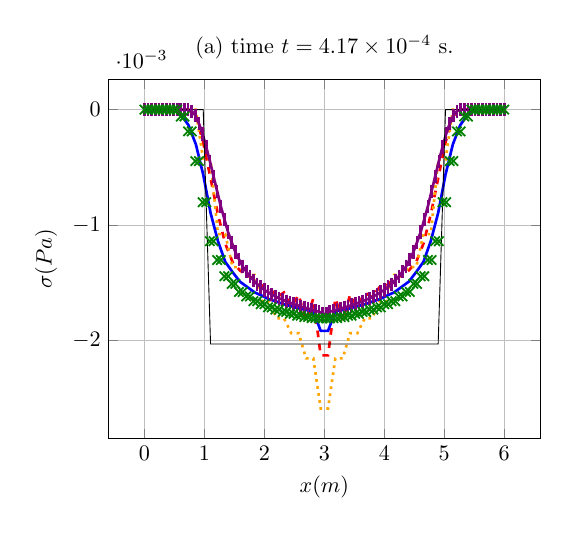
\begin{tikzpicture}[scale=0.8]
\begin{axis}[xlabel=$x (m)$,ylabel=$\sigma (Pa)$,ymajorgrids=true,xmajorgrids=true,legend pos=outer north east,title={(a) time $t = 4.17\times 10^{-4} $ s.}]
\addplot[Red,very thick,mark=none,dashed,mark size=3pt] coordinates {(0.0,0.0) (0.12244897959183673,0.0) (0.24489795918367346,0.0) (0.36734693877551017,0.0) (0.4897959183673469,0.0) (0.6122448979591837,0.0) (0.7346938775510203,-2.4706782429363735e-08) (0.8571428571428571,-5.867248412773822e-05) (0.9795918367346939,-0.0002853985909009103) (1.1020408163265305,-0.0005954308472358931) (1.2244897959183674,-0.0009067525645628951) (1.346938775510204,-0.0011607638587132671) (1.4693877551020407,-0.0013217065077757637) (1.5918367346938775,-0.001393523421223813) (1.7142857142857142,-0.0014402781682397202) (1.836734693877551,-0.001461552187294357) (1.9591836734693877,-0.0015250051575437162) (2.0816326530612246,-0.0015397083451698904) (2.204081632653061,-0.0016263965881897985) (2.326530612244898,-0.001584700145509203) (2.4489795918367347,-0.0017078111584935985) (2.571428571428571,-0.0016048877218035973) (2.693877551020408,-0.0018328835327606574) (2.816326530612245,-0.0016358851522103) (2.9387755102040813,-0.0021294274804773317) (3.061224489795918,-0.002129426547597653) (3.183673469387755,-0.0016358852194835601) (3.306122448979592,-0.0018328832921382582) (3.4285714285714284,-0.001604886057347882) (3.5510204081632653,-0.0017078117058325802) (3.673469387755102,-0.0015847007508890318) (3.7959183673469385,-0.0016263971582342353) (3.9183673469387754,-0.0015397084813633913) (4.040816326530612,-0.0015250053001396053) (4.163265306122449,-0.0014615511159168702) (4.285714285714286,-0.0014402781807440878) (4.408163265306122,-0.0013935236806247933) (4.530612244897959,-0.001321706579770408) (4.653061224489796,-0.0011607638047327214) (4.775510204081632,-0.0009067523623300537) (4.8979591836734695,-0.0005954315608474032) (5.020408163265306,-0.00028539897431746516) (5.142857142857142,-5.8672396327078764e-05) (5.26530612244898,-2.4706615951376558e-08) (5.387755102040816,0.0) (5.5102040816326525,0.0) (5.63265306122449,0.0) (5.755102040816326,0.0) (5.877551020408163,0.0) (6.0,0.0) };
\addplot[Orange,very thick,mark=none,dotted,mark size=3pt] coordinates {(0.0,0.0) (0.12244897959183673,0.0) (0.24489795918367346,0.0) (0.36734693877551017,0.0) (0.4897959183673469,0.0) (0.6122448979591837,0.0) (0.7346938775510203,-1.3329387423615422e-06) (0.8571428571428571,-1.3329399682741624e-06) (0.9795918367346939,-0.0004338120793096049) (1.1020408163265305,-0.00043381217614808966) (1.2244897959183674,-0.001078652776713751) (1.346938775510204,-0.0010786535293541098) (1.4693877551020407,-0.0013650099887886696) (1.5918367346938775,-0.0013650113404006328) (1.7142857142857142,-0.0014329121375811849) (1.836734693877551,-0.0014329136944043039) (1.9591836734693877,-0.0016624890765427765) (2.0816326530612246,-0.0016624896584601775) (2.204081632653061,-0.0018093716904116442) (2.326530612244898,-0.0018093557849666007) (2.4489795918367347,-0.001937275181781511) (2.571428571428571,-0.0019372767907533067) (2.693877551020408,-0.002155642178534488) (2.816326530612245,-0.002155640662975193) (2.9387755102040813,-0.002589762284338859) (3.061224489795918,-0.002589762175847431) (3.183673469387755,-0.002155641790343871) (3.306122448979592,-0.0021556425157575805) (3.4285714285714284,-0.0019372793251291578) (3.5510204081632653,-0.0019372778636785944) (3.673469387755102,-0.001809371471616459) (3.7959183673469385,-0.0018093710487213093) (3.9183673469387754,-0.0016624882379853954) (4.040816326530612,-0.0016624885719197634) (4.163265306122449,-0.0014329097917241942) (4.285714285714286,-0.0014329117775789128) (4.408163265306122,-0.0013650088316187207) (4.530612244897959,-0.001365009042422446) (4.653061224489796,-0.001078652980021462) (4.775510204081632,-0.001078652849949022) (4.8979591836734695,-0.00043381214864893664) (5.020408163265306,-0.0004338120674484783) (5.142857142857142,-1.3329395376771903e-06) (5.26530612244898,-1.332938627165289e-06) (5.387755102040816,0.0) (5.5102040816326525,0.0) (5.63265306122449,0.0) (5.755102040816326,0.0) (5.877551020408163,0.0) (6.0,0.0) };
\addplot[Blue,very thick,mark=none,solid,mark size=3pt] coordinates {(0.0,0.0) (0.12244897959183673,0.0) (0.24489795918367346,0.0) (0.36734693877551017,0.0) (0.4897959183673469,0.0) (0.6122448979591837,-4.674064137054689e-05) (0.7346938775510203,-0.00013518141641477002) (0.8571428571428571,-0.0003011735782562717) (0.9795918367346939,-0.0005636191184290303) (1.1020408163265305,-0.0008947918749973022) (1.2244897959183674,-0.0011384428542662672) (1.346938775510204,-0.0013187180973942406) (1.4693877551020407,-0.001408189281014569) (1.5918367346938775,-0.0014907417101391338) (1.7142857142857142,-0.001537189060000376) (1.836734693877551,-0.0015836563418978444) (1.9591836734693877,-0.0016130039487940052) (2.0816326530612246,-0.0016435577731461581) (2.204081632653061,-0.0016642561995700664) (2.326530612244898,-0.0016867439942769163) (2.4489795918367347,-0.001703774730043751) (2.571428571428571,-0.0017222255334447718) (2.693877551020408,-0.0017362714731070671) (2.816326530612245,-0.0017483096006135576) (2.9387755102040813,-0.0019170417268551047) (3.061224489795918,-0.0019170417268550973) (3.183673469387755,-0.0017483096006135571) (3.306122448979592,-0.0017362714731070667) (3.4285714285714284,-0.0017222255334447718) (3.5510204081632653,-0.001703774730043751) (3.673469387755102,-0.001686743994276917) (3.7959183673469385,-0.0016642561995700667) (3.9183673469387754,-0.0016435577731461586) (4.040816326530612,-0.001613003948794007) (4.163265306122449,-0.001583656341897845) (4.285714285714286,-0.0015371890600003768) (4.408163265306122,-0.0014907417101391342) (4.530612244897959,-0.001408189281014569) (4.653061224489796,-0.001318718097394241) (4.775510204081632,-0.0011384428542662657) (4.8979591836734695,-0.000894791874997302) (5.020408163265306,-0.0005636191184290323) (5.142857142857142,-0.00030117357825627236) (5.26530612244898,-0.0001351814164147703) (5.387755102040816,-4.674064137054787e-05) (5.5102040816326525,0.0) (5.63265306122449,0.0) (5.755102040816326,0.0) (5.877551020408163,0.0) (6.0,0.0) };
\addplot[Purple,very thick,mark=|,solid,mark size=3pt] coordinates {(0.0,0.0) (0.06060606060606061,0.0) (0.12121212121212122,0.0) (0.18181818181818182,0.0) (0.24242424242424243,0.0) (0.30303030303030304,0.0) (0.36363636363636365,0.0) (0.42424242424242425,0.0) (0.48484848484848486,0.0) (0.5454545454545454,0.0) (0.6060606060606061,0.0) (0.6666666666666667,-4.0531023418027623e-11) (0.7272727272727273,-9.569933907036341e-07) (0.7878787878787878,-1.343261689597016e-05) (0.8484848484848485,-4.9558531577573574e-05) (0.9090909090909092,-0.00012085333050559284) (0.9696969696969697,-0.00021200690708122615) (1.0303030303030303,-0.0003243493959749349) (1.0909090909090908,-0.0004471679110108456) (1.1515151515151516,-0.0005777044805089968) (1.2121212121212122,-0.0007079212371215294) (1.2727272727272727,-0.0008366965691899573) (1.3333333333333335,-0.0009513341656497712) (1.393939393939394,-0.0010611178168264638) (1.4545454545454546,-0.0011492229400598727) (1.5151515151515151,-0.0012334657955739342) (1.5757575757575757,-0.0012964181089512702) (1.6363636363636365,-0.0013579641179089666) (1.696969696969697,-0.0014023349566352568) (1.7575757575757576,-0.0014472561599906432) (1.8181818181818183,-0.0014792542904296902) (1.878787878787879,-0.0015129085145436797) (1.9393939393939394,-0.001536820399711865) (2.0,-0.0015629352013383615) (2.0606060606060606,-0.001581443333690898) (2.121212121212121,-0.0016024369422373745) (2.1818181818181817,-0.0016172073793473665) (2.2424242424242427,-0.0016346556959052913) (2.303030303030303,-0.0016467496593637076) (2.3636363636363638,-0.0016617233860291073) (2.4242424242424243,-0.0016718388130052982) (2.484848484848485,-0.0016851233861680903) (2.5454545454545454,-0.0016937313987460364) (2.606060606060606,-0.0017059907853383823) (2.666666666666667,-0.0017134098017108522) (2.7272727272727275,-0.0017253826926178872) (2.787878787878788,-0.0017318058838217147) (2.8484848484848486,-0.0017448175639310159) (2.909090909090909,-0.00175019771707795) (2.9696969696969697,-0.0017717316670483852) (3.0303030303030303,-0.0017717316670483854) (3.090909090909091,-0.00175019771707795) (3.1515151515151514,-0.0017448175639310163) (3.2121212121212124,-0.001731805883821715) (3.272727272727273,-0.0017253826926178879) (3.3333333333333335,-0.001713409801710852) (3.393939393939394,-0.0017059907853383828) (3.4545454545454546,-0.001693731398746037) (3.515151515151515,-0.001685123386168091) (3.5757575757575757,-0.0016718388130052986) (3.6363636363636367,-0.0016617233860291081) (3.6969696969696972,-0.001646749659363708) (3.757575757575758,-0.001634655695905292) (3.8181818181818183,-0.0016172073793473672) (3.878787878787879,-0.0016024369422373756) (3.9393939393939394,-0.001581443333690899) (4.0,-0.0015629352013383628) (4.0606060606060606,-0.0015368203997118664) (4.121212121212121,-0.0015129085145436816) (4.181818181818182,-0.0014792542904296917) (4.242424242424242,-0.001447256159990645) (4.303030303030303,-0.0014023349566352596) (4.363636363636363,-0.00135796411790897) (4.424242424242425,-0.0012964181089512726) (4.484848484848485,-0.001233465795573936) (4.545454545454546,-0.0011492229400598753) (4.606060606060606,-0.0010611178168264672) (4.666666666666667,-0.0009513341656497752) (4.7272727272727275,-0.000836696569189961) (4.787878787878788,-0.0007079212371215326) (4.848484848484849,-0.0005777044805089981) (4.909090909090909,-0.00044716791101084754) (4.96969696969697,-0.00032434939597493647) (5.03030303030303,-0.0002120069070812274) (5.090909090909091,-0.00012085333050559367) (5.151515151515151,-4.955853157757462e-05) (5.212121212121212,-1.3432616895970462e-05) (5.2727272727272725,-9.56993390703686e-07) (5.333333333333334,-4.0531023418038635e-11) (5.3939393939393945,0.0) (5.454545454545455,0.0) (5.515151515151516,0.0) (5.575757575757576,0.0) (5.636363636363637,0.0) (5.696969696969697,0.0) (5.757575757575758,0.0) (5.818181818181818,0.0) (5.878787878787879,0.0) (5.9393939393939394,0.0) (6.0,0.0) };
\addplot[Green,thick,mark=x,only marks,mark size=3pt] coordinates {(0.0,0.0) (0.06060606060606061,0.0) (0.12121212121212122,0.0) (0.18181818181818182,0.0) (0.24242424242424243,0.0) (0.30303030303030304,0.0) (0.36363636363636365,0.0) (0.42424242424242425,0.0) (0.48484848484848486,0.0) (0.5454545454545454,0.0) (0.6060606060606061,-5.95994308592662e-05) (0.6666666666666667,-5.959943085926653e-05) (0.7272727272727273,-0.00018884662936873652) (0.7878787878787878,-0.00018884662936873706) (0.8484848484848485,-0.0004463332330303008) (0.9090909090909092,-0.00044633323303030104) (0.9696969696969697,-0.0008024468949020794) (1.0303030303030303,-0.0008024468949020728) (1.0909090909090908,-0.0011402025229616407) (1.1515151515151516,-0.0011402025229616413) (1.2121212121212122,-0.001303374963621311) (1.2727272727272727,-0.0013033749636213118) (1.3333333333333335,-0.0014435674663425906) (1.393939393939394,-0.0014435674663425915) (1.4545454545454546,-0.0015100315038270278) (1.5151515151515151,-0.0015100315038270632) (1.5757575757575757,-0.0015802302171187615) (1.6363636363636365,-0.0015802302171187552) (1.696969696969697,-0.0016188693449786943) (1.7575757575757576,-0.0016188693449786839) (1.8181818181818183,-0.0016602445166918156) (1.878787878787879,-0.0016602445166918167) (1.9393939393939394,-0.0016861774822787279) (2.0,-0.0016861774822787287) (2.0606060606060606,-0.0017138047010635522) (2.121212121212121,-0.0017138047010635828) (2.1818181818181817,-0.001733009016979971) (2.2424242424242427,-0.001733009016980024) (2.303030303030303,-0.0017535801619425328) (2.3636363636363638,-0.0017535801619425221) (2.4242424242424243,-0.0017693554459473537) (2.484848484848485,-0.001769355445947317) (2.5454545454545454,-0.0017856035728642274) (2.606060606060606,-0.0017856035728642042) (2.666666666666667,-0.0017976908098995877) (2.7272727272727275,-0.0017976908098995808) (2.787878787878788,-0.001806107529340324) (2.8484848484848486,-0.001806107529340337) (2.909090909090909,-0.0018091152724179298) (2.9696969696969697,-0.0018091152724178296) (3.0303030303030303,-0.001809115272417879) (3.090909090909091,-0.001809115272417851) (3.1515151515151514,-0.0018061075293403382) (3.2121212121212124,-0.0018061075293403603) (3.272727272727273,-0.0017976908098994923) (3.3333333333333335,-0.0017976908098994875) (3.393939393939394,-0.0017856035728641474) (3.4545454545454546,-0.0017856035728641513) (3.515151515151515,-0.0017693554459472887) (3.5757575757575757,-0.0017693554459472952) (3.6363636363636367,-0.0017535801619425245) (3.6969696969696972,-0.0017535801619425078) (3.757575757575758,-0.0017330090169799064) (3.8181818181818183,-0.0017330090169799365) (3.878787878787879,-0.0017138047010635275) (3.9393939393939394,-0.0017138047010634284) (4.0,-0.0016861774822786698) (4.0606060606060606,-0.0016861774822786624) (4.121212121212121,-0.0016602445166917154) (4.181818181818182,-0.0016602445166917187) (4.242424242424242,-0.0016188693449785446) (4.303030303030303,-0.0016188693449785436) (4.363636363636363,-0.001580230217118671) (4.424242424242425,-0.0015802302171186698) (4.484848484848485,-0.0015100315038270133) (4.545454545454546,-0.0015100315038270502) (4.606060606060606,-0.0014435674663425381) (4.666666666666667,-0.0014435674663425414) (4.7272727272727275,-0.0013033749636212864) (4.787878787878788,-0.0013033749636212884) (4.848484848484849,-0.0011402025229617428) (4.909090909090909,-0.0011402025229617456) (4.96969696969697,-0.0008024468949021485) (5.03030303030303,-0.0008024468949021475) (5.090909090909091,-0.000446333233030326) (5.151515151515151,-0.0004463332330303249) (5.212121212121212,-0.00018884662936874592) (5.2727272727272725,-0.00018884662936874598) (5.333333333333334,-5.95994308592702e-05) (5.3939393939393945,-5.959943085927111e-05) (5.454545454545455,0.0) (5.515151515151516,0.0) (5.575757575757576,0.0) (5.636363636363637,0.0) (5.696969696969697,0.0) (5.757575757575758,0.0) (5.818181818181818,0.0) (5.878787878787879,0.0) (5.9393939393939394,0.0) (6.0,0.0) };
\addplot[black,thin,mark=none,solid,mark size=3pt] coordinates {(0.0,-0.0) (0.12244897959183673,-0.0) (0.24489795918367346,-0.0) (0.36734693877551017,-0.0) (0.4897959183673469,-0.0) (0.6122448979591837,-0.0) (0.7346938775510203,-0.0) (0.8571428571428571,-0.0) (0.9795918367346939,-0.0) (1.1020408163265305,-0.002030785796418313) (1.2244897959183674,-0.002030785796418313) (1.346938775510204,-0.002030785796418313) (1.4693877551020407,-0.002030785796418313) (1.5918367346938775,-0.002030785796418313) (1.7142857142857142,-0.002030785796418313) (1.836734693877551,-0.002030785796418313) (1.9591836734693877,-0.002030785796418313) (2.0816326530612246,-0.002030785796418313) (2.204081632653061,-0.002030785796418313) (2.326530612244898,-0.002030785796418313) (2.4489795918367347,-0.002030785796418313) (2.571428571428571,-0.002030785796418313) (2.693877551020408,-0.002030785796418313) (2.816326530612245,-0.002030785796418313) (2.9387755102040813,-0.002030785796418313) (3.061224489795918,-0.002030785796418313) (3.183673469387755,-0.002030785796418313) (3.306122448979592,-0.002030785796418313) (3.4285714285714284,-0.002030785796418313) (3.5510204081632653,-0.002030785796418313) (3.673469387755102,-0.002030785796418313) (3.7959183673469385,-0.002030785796418313) (3.9183673469387754,-0.002030785796418313) (4.040816326530612,-0.002030785796418313) (4.163265306122449,-0.002030785796418313) (4.285714285714286,-0.002030785796418313) (4.408163265306122,-0.002030785796418313) (4.530612244897959,-0.002030785796418313) (4.653061224489796,-0.002030785796418313) (4.775510204081632,-0.002030785796418313) (4.8979591836734695,-0.002030785796418313) (5.020408163265306,-0.0) (5.142857142857142,-0.0) (5.26530612244898,-0.0) (5.387755102040816,-0.0) (5.5102040816326525,-0.0) (5.63265306122449,-0.0) (5.755102040816326,-0.0) (5.877551020408163,-0.0) (6.0,-0.0) };
%\legend{usl 1ppc,usf 1ppc,dgmpm 1ppc,dgmpm 2ppc,dgmpm 2ppc (RK2 + strang),plastic solution}
\end{axis}
\end{tikzpicture}
%%% Local Variables:
%%% mode: latex
%%% TeX-master: "../../mainManuscript"
%%% End:
}
%   {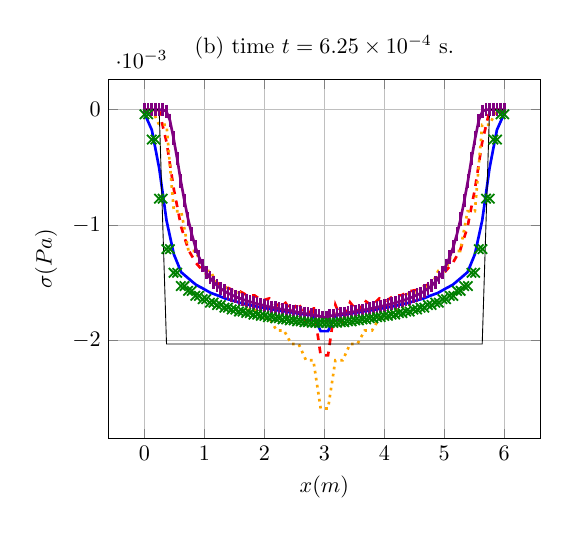
\begin{tikzpicture}[scale=0.8]
\begin{axis}[xlabel=$x (m)$,ylabel=$\sigma (Pa)$,ymajorgrids=true,xmajorgrids=true,legend pos=outer north east,title={(b) time $t = 6.25\times 10^{-4} $ s.}]
\addplot[Red,very thick,mark=none,dashed,mark size=3pt] coordinates {(0.0,0.0) (0.12244897959183673,0.0) (0.24489795918367346,-9.09743714498828e-06) (0.36734693877551017,-0.00028060178384402246) (0.4897959183673469,-0.000690645014524663) (0.6122448979591837,-0.0010172754869474821) (0.7346938775510203,-0.0012174879404668873) (0.8571428571428571,-0.001327790359856718) (0.9795918367346939,-0.0014002058405938708) (1.1020408163265305,-0.0014574762656029724) (1.2244897959183674,-0.001505353831791513) (1.346938775510204,-0.0015338005451529275) (1.4693877551020407,-0.0015635221192807454) (1.5918367346938775,-0.0015753991257001431) (1.7142857142857142,-0.0016098352308080907) (1.836734693877551,-0.0016105966109038212) (1.9591836734693877,-0.0016554023072314432) (2.0816326530612246,-0.0016360935152320186) (2.204081632653061,-0.0016986137246127954) (2.326530612244898,-0.0016550171076523833) (2.4489795918367347,-0.0017506128422217714) (2.571428571428571,-0.001670222601515723) (2.693877551020408,-0.001843959044053449) (2.816326530612245,-0.0016915571845227079) (2.9387755102040813,-0.002129427489038802) (3.061224489795918,-0.0021294265561618607) (3.183673469387755,-0.0016915572429560084) (3.306122448979592,-0.0018439587286891077) (3.4285714285714284,-0.0016702218101354916) (3.5510204081632653,-0.001750613256004356) (3.673469387755102,-0.0016550174088773542) (3.7959183673469385,-0.001698614023304057) (3.9183673469387754,-0.0016360936167129818) (4.040816326530612,-0.0016554021914399486) (4.163265306122449,-0.0016105964191050952) (4.285714285714286,-0.0016098352679559734) (4.408163265306122,-0.0015753992486767384) (4.530612244897959,-0.0015635221977266104) (4.653061224489796,-0.0015338005571043653) (4.775510204081632,-0.0015053538409978895) (4.8979591836734695,-0.001457476331976043) (5.020408163265306,-0.001400205486223803) (5.142857142857142,-0.0013277905131784619) (5.26530612244898,-0.0012174886002592263) (5.387755102040816,-0.0010172757767319969) (5.5102040816326525,-0.0006906448932635886) (5.63265306122449,-0.0002806022282810553) (5.755102040816326,-9.097387796699236e-06) (5.877551020408163,0.0) (6.0,0.0) };
\addplot[Orange,very thick,mark=none,dotted,mark size=3pt] coordinates {(0.0,0.0) (0.12244897959183673,0.0) (0.24489795918367346,-0.00013125567272782819) (0.36734693877551017,-0.00013125591615145197) (0.4897959183673469,-0.0008813832603320562) (0.6122448979591837,-0.0008813838642660081) (0.7346938775510203,-0.0012247428359422696) (0.8571428571428571,-0.0012247425724953693) (0.9795918367346939,-0.001397689841428779) (1.1020408163265305,-0.0013976897509958288) (1.2244897959183674,-0.001536227538045054) (1.346938775510204,-0.001536227937408319) (1.4693877551020407,-0.0015850329963259663) (1.5918367346938775,-0.0015850318594526924) (1.7142857142857142,-0.0017348225074951447) (1.836734693877551,-0.0017348212862825618) (1.9591836734693877,-0.0018063592675864129) (2.0816326530612246,-0.001806359731310172) (2.204081632653061,-0.0019134829069542122) (2.326530612244898,-0.0019134752699114365) (2.4489795918367347,-0.0020308300009669426) (2.571428571428571,-0.0020308316942653946) (2.693877551020408,-0.0021721534919969363) (2.816326530612245,-0.0021721522612295503) (2.9387755102040813,-0.002589832926025744) (3.061224489795918,-0.0025898328149225646) (3.183673469387755,-0.002172153099923732) (3.306122448979592,-0.002172153496185014) (3.4285714285714284,-0.0020308319106928136) (3.5510204081632653,-0.002030831353584487) (3.673469387755102,-0.0019134829101521314) (3.7959183673469385,-0.0019134826107273153) (3.9183673469387754,-0.0018063586181389377) (4.040816326530612,-0.0018063592789159533) (4.163265306122449,-0.001734821842983902) (4.285714285714286,-0.0017348222168737536) (4.408163265306122,-0.0015850322909855233) (4.530612244897959,-0.0015850322551182372) (4.653061224489796,-0.0015362286519360463) (4.775510204081632,-0.0015362274905299917) (4.8979591836734695,-0.0013976888757025222) (5.020408163265306,-0.0013976898142422994) (5.142857142857142,-0.0012247427216731783) (5.26530612244898,-0.0012247427719878296) (5.387755102040816,-0.0008813837524078346) (5.5102040816326525,-0.000881379580518873) (5.63265306122449,-0.00013125562655680082) (5.755102040816326,-0.0001312556126026732) (5.877551020408163,0.0) (6.0,0.0) };
\addplot[Blue,very thick,mark=none,solid,mark size=3pt] coordinates {(0.0,-3.288656606774586e-05) (0.12244897959183673,-0.00017641909201459894) (0.24489795918367346,-0.000506646129358451) (0.36734693877551017,-0.0009600605637646077) (0.4897959183673469,-0.001253427110389605) (0.6122448979591837,-0.0014089288532961235) (0.7346938775510203,-0.0014636954486616234) (0.8571428571428571,-0.0015173032590703268) (0.9795918367346939,-0.001551337471828278) (1.1020408163265305,-0.0015875427344901954) (1.2244897959183674,-0.0016109960299248184) (1.346938775510204,-0.0016369488867646299) (1.4693877551020407,-0.0016544898328871023) (1.5918367346938775,-0.0016739161084835994) (1.7142857142857142,-0.001687923915138772) (1.836734693877551,-0.0017030619275038906) (1.9591836734693877,-0.0017147494357043645) (2.0816326530612246,-0.0017269459689745993) (2.204081632653061,-0.0017370154541442267) (2.326530612244898,-0.001747456536468629) (2.4489795918367347,-0.0017569942648830645) (2.571428571428571,-0.0017669191588267057) (2.693877551020408,-0.0017756679773472232) (2.816326530612245,-0.0017829750209496743) (2.9387755102040813,-0.0019198249761128202) (3.061224489795918,-0.001919824976112813) (3.183673469387755,-0.001782975020949674) (3.306122448979592,-0.0017756679773472232) (3.4285714285714284,-0.001766919158826706) (3.5510204081632653,-0.0017569942648830654) (3.673469387755102,-0.0017474565364686298) (3.7959183673469385,-0.0017370154541442278) (3.9183673469387754,-0.0017269459689746) (4.040816326530612,-0.0017147494357043658) (4.163265306122449,-0.0017030619275038915) (4.285714285714286,-0.0016879239151387725) (4.408163265306122,-0.0016739161084836) (4.530612244897959,-0.0016544898328871031) (4.653061224489796,-0.001636948886764631) (4.775510204081632,-0.0016109960299248193) (4.8979591836734695,-0.001587542734490196) (5.020408163265306,-0.0015513374718282788) (5.142857142857142,-0.0015173032590703277) (5.26530612244898,-0.0014636954486616236) (5.387755102040816,-0.0014089288532961226) (5.5102040816326525,-0.0012534271103896038) (5.63265306122449,-0.000960060563764606) (5.755102040816326,-0.0005066461293584512) (5.877551020408163,-0.00017641909201459888) (6.0,-3.2886566067745944e-05) };
\addplot[Purple,very thick,mark=|,solid,mark size=3pt] coordinates {(0.0,0.0) (0.06060606060606061,0.0) (0.12121212121212122,0.0) (0.18181818181818182,0.0) (0.24242424242424243,0.0) (0.30303030303030304,-1.192012716404481e-07) (0.36363636363636365,-1.4562449689300448e-05) (0.42424242424242425,-9.236457975705467e-05) (0.48484848484848486,-0.0002470376030914057) (0.5454545454545454,-0.000425718225432667) (0.6060606060606061,-0.0006194023809233477) (0.6666666666666667,-0.0007903226149766369) (0.7272727272727273,-0.0009484637233093347) (0.7878787878787878,-0.001077982039857484) (0.8484848484848485,-0.0011884743153909919) (0.9090909090909092,-0.001277319324857129) (0.9696969696969697,-0.0013502507843687374) (1.0303030303030303,-0.0014093248881660956) (1.0909090909090908,-0.001456586468333663) (1.1515151515151516,-0.0014954551893398439) (1.2121212121212122,-0.0015258020679790962) (1.2727272727272727,-0.0015519977804941763) (1.3333333333333335,-0.0015722461442494063) (1.393939393939394,-0.0015911837536253385) (1.4545454545454546,-0.0016058566241831974) (1.5151515151515151,-0.0016207034860120757) (1.5757575757575757,-0.0016322577806829907) (1.6363636363636365,-0.0016446308515186924) (1.696969696969697,-0.0016542659958777353) (1.7575757575757576,-0.0016649744154638819) (1.8181818181818183,-0.0016732800734457133) (1.878787878787879,-0.0016827672710207039) (1.9393939393939394,-0.0016900659440740899) (2.0,-0.0016986145006445332) (2.0606060606060606,-0.0017051104495914072) (2.121212121212121,-0.0017129279540977528) (2.1818181818181817,-0.0017187667900267708) (2.2424242424242427,-0.0017260236649975474) (2.303030303030303,-0.0017313165739623365) (2.3636363636363638,-0.0017381681294236975) (2.4242424242424243,-0.0017430027538714655) (2.484848484848485,-0.0017496107790071042) (2.5454545454545454,-0.0017540562886207848) (2.606060606060606,-0.0017606250777175883) (2.666666666666667,-0.0017647324970514386) (2.7272727272727275,-0.0017715990863667725) (2.787878787878788,-0.0017753916177228703) (2.8484848484848486,-0.0017833572523661626) (2.909090909090909,-0.0017867388502595498) (2.9696969696969697,-0.0018009642034702022) (3.0303030303030303,-0.0018009642034702024) (3.090909090909091,-0.0017867388502595498) (3.1515151515151514,-0.0017833572523661633) (3.2121212121212124,-0.0017753916177228705) (3.272727272727273,-0.0017715990863667731) (3.3333333333333335,-0.0017647324970514388) (3.393939393939394,-0.0017606250777175893) (3.4545454545454546,-0.0017540562886207858) (3.515151515151515,-0.0017496107790071053) (3.5757575757575757,-0.0017430027538714663) (3.6363636363636367,-0.0017381681294236994) (3.6969696969696972,-0.0017313165739623376) (3.757575757575758,-0.0017260236649975485) (3.8181818181818183,-0.0017187667900267715) (3.878787878787879,-0.0017129279540977545) (3.9393939393939394,-0.0017051104495914087) (4.0,-0.0016986145006445343) (4.0606060606060606,-0.0016900659440740914) (4.121212121212121,-0.0016827672710207056) (4.181818181818182,-0.001673280073445715) (4.242424242424242,-0.0016649744154638838) (4.303030303030303,-0.0016542659958777375) (4.363636363636363,-0.0016446308515186954) (4.424242424242425,-0.0016322577806829933) (4.484848484848485,-0.0016207034860120783) (4.545454545454546,-0.0016058566241832003) (4.606060606060606,-0.001591183753625341) (4.666666666666667,-0.0015722461442494097) (4.7272727272727275,-0.001551997780494179) (4.787878787878788,-0.0015258020679791) (4.848484848484849,-0.0014954551893398465) (4.909090909090909,-0.0014565864683336663) (4.96969696969697,-0.0014093248881660982) (5.03030303030303,-0.0013502507843687402) (5.090909090909091,-0.0012773193248571315) (5.151515151515151,-0.001188474315390994) (5.212121212121212,-0.001077982039857487) (5.2727272727272725,-0.0009484637233093383) (5.333333333333334,-0.0007903226149766394) (5.3939393939393945,-0.0006194023809233497) (5.454545454545455,-0.00042571822543266863) (5.515151515151516,-0.000247037603091407) (5.575757575757576,-9.236457975705492e-05) (5.636363636363637,-1.4562449689300525e-05) (5.696969696969697,-1.1920127164044906e-07) (5.757575757575758,0.0) (5.818181818181818,0.0) (5.878787878787879,0.0) (5.9393939393939394,0.0) (6.0,0.0) };
\addplot[Green,thick,mark=x,only marks,mark size=3pt] coordinates {(0.0,-4.077076000132571e-05) (0.06060606060606061,-4.077076000132737e-05) (0.12121212121212122,-0.000259465833593339) (0.18181818181818182,-0.0002594658335933402) (0.24242424242424243,-0.0007718131581974564) (0.30303030303030304,-0.0007718131581974544) (0.36363636363636365,-0.0012089832811266732) (0.42424242424242425,-0.0012089832811266726) (0.48484848484848486,-0.0014141342215499664) (0.5454545454545454,-0.001414134221549973) (0.6060606060606061,-0.0015288994593393016) (0.6666666666666667,-0.0015288994593392992) (0.7272727272727273,-0.001570800224198939) (0.7878787878787878,-0.0015708002241989342) (0.8484848484848485,-0.0016141244026557006) (0.9090909090909092,-0.0016141244026557173) (0.9696969696969697,-0.0016423561224507385) (1.0303030303030303,-0.0016423561224507043) (1.0909090909090908,-0.0016729153381830181) (1.1515151515151516,-0.0016729153381830314) (1.2121212121212122,-0.0016934523002053714) (1.2727272727272727,-0.0016934523002054237) (1.3333333333333335,-0.001716262292786097) (1.393939393939394,-0.0017162622927860622) (1.4545454545454546,-0.0017321137630453758) (1.5151515151515151,-0.0017321137630453532) (1.5757575757575757,-0.0017497799126621094) (1.6363636363636365,-0.0017497799126621125) (1.696969696969697,-0.0017625571698028399) (1.7575757575757576,-0.0017625571698028355) (1.8181818181818183,-0.001776558904084057) (1.878787878787879,-0.0017765589040840486) (1.9393939393939394,-0.0017871695859244035) (2.0,-0.0017871695859243287) (2.0606060606060606,-0.0017985263217785796) (2.121212121212121,-0.0017985263217786393) (2.1818181818181817,-0.0018077111881619988) (2.2424242424242427,-0.0018077111881619735) (2.303030303030303,-0.0018174288517170986) (2.3636363636363638,-0.0018174288517171257) (2.4242424242424243,-0.0018259390176408893) (2.484848484848485,-0.0018259390176408438) (2.5454545454545454,-0.001834601910130878) (2.606060606060606,-0.00183460191013079) (2.666666666666667,-0.0018417911948099834) (2.7272727272727275,-0.0018417911948099739) (2.787878787878788,-0.0018466992729078942) (2.8484848484848486,-0.001846699272907896) (2.909090909090909,-0.0018486141474135926) (2.9696969696969697,-0.001848614147413537) (3.0303030303030303,-0.001848614147413566) (3.090909090909091,-0.0018486141474135737) (3.1515151515151514,-0.001846699272907917) (3.2121212121212124,-0.001846699272907892) (3.272727272727273,-0.0018417911948100014) (3.3333333333333335,-0.0018417911948099752) (3.393939393939394,-0.001834601910130857) (3.4545454545454546,-0.0018346019101308337) (3.515151515151515,-0.0018259390176409316) (3.5757575757575757,-0.001825939017640955) (3.6363636363636367,-0.0018174288517171517) (3.6969696969696972,-0.0018174288517170893) (3.757575757575758,-0.001807711188161973) (3.8181818181818183,-0.0018077111881620055) (3.878787878787879,-0.001798526321778638) (3.9393939393939394,-0.001798526321778626) (4.0,-0.001787169585924375) (4.0606060606060606,-0.0017871695859243203) (4.121212121212121,-0.0017765589040840638) (4.181818181818182,-0.0017765589040839964) (4.242424242424242,-0.0017625571698028266) (4.303030303030303,-0.0017625571698028134) (4.363636363636363,-0.0017497799126621459) (4.424242424242425,-0.001749779912662138) (4.484848484848485,-0.0017321137630453144) (4.545454545454546,-0.0017321137630453304) (4.606060606060606,-0.0017162622927860659) (4.666666666666667,-0.0017162622927860381) (4.7272727272727275,-0.0016934523002054068) (4.787878787878788,-0.0016934523002054246) (4.848484848484849,-0.0016729153381829882) (4.909090909090909,-0.001672915338182986) (4.96969696969697,-0.001642356122450608) (5.03030303030303,-0.001642356122450549) (5.090909090909091,-0.0016141244026555914) (5.151515151515151,-0.001614124402655621) (5.212121212121212,-0.0015708002241988284) (5.2727272727272725,-0.0015708002241988448) (5.333333333333334,-0.0015288994593392303) (5.3939393939393945,-0.001528899459339235) (5.454545454545455,-0.0014141342215499202) (5.515151515151516,-0.001414134221549916) (5.575757575757576,-0.0012089832811266546) (5.636363636363637,-0.001208983281126654) (5.696969696969697,-0.000771813158197516) (5.757575757575758,-0.000771813158197514) (5.818181818181818,-0.0002594658335933476) (5.878787878787879,-0.00025946583359334876) (5.9393939393939394,-4.0770760001336276e-05) (6.0,-4.077076000133824e-05) };
\addplot[black,thin,mark=none,solid,mark size=3pt] coordinates {(0.0,-0.0) (0.12244897959183673,-0.0) (0.24489795918367346,-0.0) (0.36734693877551017,-0.002030785796418313) (0.4897959183673469,-0.002030785796418313) (0.6122448979591837,-0.002030785796418313) (0.7346938775510203,-0.002030785796418313) (0.8571428571428571,-0.002030785796418313) (0.9795918367346939,-0.002030785796418313) (1.1020408163265305,-0.002030785796418313) (1.2244897959183674,-0.002030785796418313) (1.346938775510204,-0.002030785796418313) (1.4693877551020407,-0.002030785796418313) (1.5918367346938775,-0.002030785796418313) (1.7142857142857142,-0.002030785796418313) (1.836734693877551,-0.002030785796418313) (1.9591836734693877,-0.002030785796418313) (2.0816326530612246,-0.002030785796418313) (2.204081632653061,-0.002030785796418313) (2.326530612244898,-0.002030785796418313) (2.4489795918367347,-0.002030785796418313) (2.571428571428571,-0.002030785796418313) (2.693877551020408,-0.002030785796418313) (2.816326530612245,-0.002030785796418313) (2.9387755102040813,-0.002030785796418313) (3.061224489795918,-0.002030785796418313) (3.183673469387755,-0.002030785796418313) (3.306122448979592,-0.002030785796418313) (3.4285714285714284,-0.002030785796418313) (3.5510204081632653,-0.002030785796418313) (3.673469387755102,-0.002030785796418313) (3.7959183673469385,-0.002030785796418313) (3.9183673469387754,-0.002030785796418313) (4.040816326530612,-0.002030785796418313) (4.163265306122449,-0.002030785796418313) (4.285714285714286,-0.002030785796418313) (4.408163265306122,-0.002030785796418313) (4.530612244897959,-0.002030785796418313) (4.653061224489796,-0.002030785796418313) (4.775510204081632,-0.002030785796418313) (4.8979591836734695,-0.002030785796418313) (5.020408163265306,-0.002030785796418313) (5.142857142857142,-0.002030785796418313) (5.26530612244898,-0.002030785796418313) (5.387755102040816,-0.002030785796418313) (5.5102040816326525,-0.002030785796418313) (5.63265306122449,-0.002030785796418313) (5.755102040816326,-0.0) (5.877551020408163,-0.0) (6.0,-0.0) };
%\legend{usl 1ppc,usf 1ppc,dgmpm 1ppc,dgmpm 2ppc,dgmpm 2ppc (RK2 + strang),plastic solution}
\end{axis}
\end{tikzpicture}
%%% Local Variables:
%%% mode: latex
%%% TeX-master: "../../mainManuscript"
%%% End:
}
%   {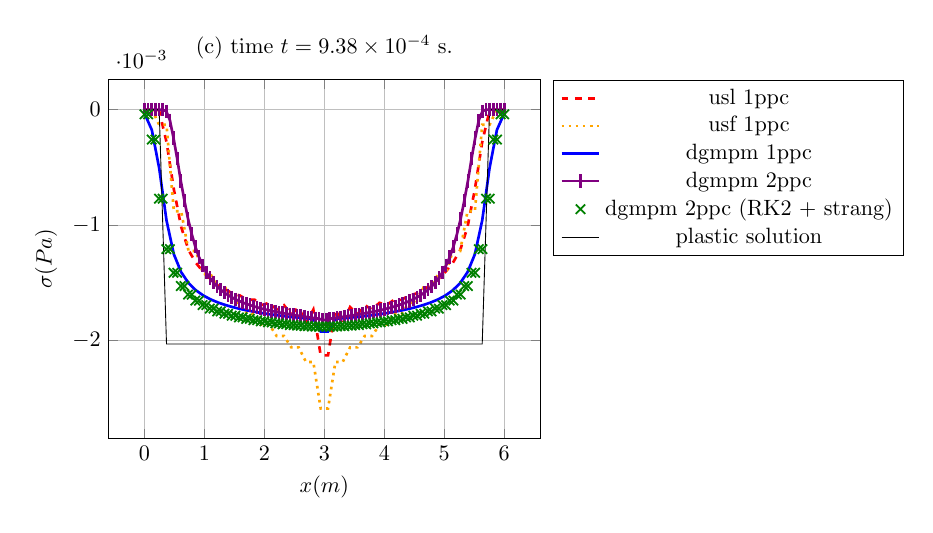
\begin{tikzpicture}[scale=0.8]
\begin{axis}[xlabel=$x (m)$,ylabel=$\sigma (Pa)$,ymajorgrids=true,xmajorgrids=true,legend pos=outer north east,title={(c) time $t = 9.38\times 10^{-4} $ s.}]
\addplot[Red,very thick,mark=none,dashed,mark size=3pt] coordinates {(0.0,0.0) (0.12244897959183673,0.0) (0.24489795918367346,-9.09743714498828e-06) (0.36734693877551017,-0.00028060178384402246) (0.4897959183673469,-0.000690645014524663) (0.6122448979591837,-0.0010172754869474821) (0.7346938775510203,-0.0012174879404668873) (0.8571428571428571,-0.0013280180462532844) (0.9795918367346939,-0.001405573314687709) (1.1020408163265305,-0.0014715381825829389) (1.2244897959183674,-0.0015240182188866489) (1.346938775510204,-0.0015561890073244227) (1.4693877551020407,-0.0015945318145481168) (1.5918367346938775,-0.0016110732006773488) (1.7142857142857142,-0.0016486349228612136) (1.836734693877551,-0.0016475965034896671) (1.9591836734693877,-0.0016928166346279892) (2.0816326530612246,-0.001674127735672926) (2.204081632653061,-0.0017324385481802082) (2.326530612244898,-0.0016946099760850012) (2.4489795918367347,-0.0017749462373902935) (2.571428571428571,-0.0017118415467530894) (2.693877551020408,-0.0018524608793206972) (2.816326530612245,-0.0017331235724179987) (2.9387755102040813,-0.0021294274890493736) (3.061224489795918,-0.0021294265561724456) (3.183673469387755,-0.0017331236195573326) (3.306122448979592,-0.001852460536357857) (3.4285714285714284,-0.0017118410940132381) (3.5510204081632653,-0.0017749465825430376) (3.673469387755102,-0.0016946101804939575) (3.7959183673469385,-0.0017324387664782147) (3.9183673469387754,-0.0016741278276934143) (4.040816326530612,-0.0016928165624296699) (4.163265306122449,-0.00164759638416514) (4.285714285714286,-0.0016486349315771296) (4.408163265306122,-0.0016110732691248558) (4.530612244897959,-0.0015945318680601172) (4.653061224489796,-0.001556189037305485) (4.775510204081632,-0.001524018258266158) (4.8979591836734695,-0.0014715382275786231) (5.020408163265306,-0.001405572961530602) (5.142857142857142,-0.0013280181972431424) (5.26530612244898,-0.0012174886002592263) (5.387755102040816,-0.0010172757767319969) (5.5102040816326525,-0.0006906448932635886) (5.63265306122449,-0.0002806022282810553) (5.755102040816326,-9.097387796699236e-06) (5.877551020408163,0.0) (6.0,0.0) };
\addplot[Orange,very thick,mark=none,dotted,mark size=3pt] coordinates {(0.0,0.0) (0.12244897959183673,0.0) (0.24489795918367346,-0.00013125567272782819) (0.36734693877551017,-0.00013125591615145197) (0.4897959183673469,-0.0008813832603320562) (0.6122448979591837,-0.0008813838642660081) (0.7346938775510203,-0.0012247851551192936) (0.8571428571428571,-0.001224784890440556) (0.9795918367346939,-0.0014249339778741803) (1.1020408163265305,-0.0014249341228939742) (1.2244897959183674,-0.0015414554008737465) (1.346938775510204,-0.0015414557554649711) (1.4693877551020407,-0.0016738699379305296) (1.5918367346938775,-0.0016738690962649337) (1.7142857142857142,-0.0017713609761048244) (1.836734693877551,-0.0017713599892547082) (1.9591836734693877,-0.0018625169761770728) (2.0816326530612246,-0.0018625172930377735) (2.204081632653061,-0.001961668570283414) (2.326530612244898,-0.0019616634232208813) (2.4489795918367347,-0.0020602990364256483) (2.571428571428571,-0.002060300428159983) (2.693877551020408,-0.0021870752843109642) (2.816326530612245,-0.002187074359760412) (2.9387755102040813,-0.0025898336000690844) (3.061224489795918,-0.002589833489024399) (3.183673469387755,-0.0021870749435822555) (3.306122448979592,-0.002187075320243097) (3.4285714285714284,-0.0020603004028730636) (3.5510204081632653,-0.002060299945635322) (3.673469387755102,-0.001961668579229524) (3.7959183673469385,-0.0019616680989035505) (3.9183673469387754,-0.0018625166965802594) (4.040816326530612,-0.0018625168203206587) (4.163265306122449,-0.0017713603337100934) (4.285714285714286,-0.0017713606793835414) (4.408163265306122,-0.0016738693883742992) (4.530612244897959,-0.0016738697730550773) (4.653061224489796,-0.0015414564688055982) (4.775510204081632,-0.0015414554924597567) (4.8979591836734695,-0.0014249331462970946) (5.020408163265306,-0.0014249341572060055) (5.142857142857142,-0.0012247850399668774) (5.26530612244898,-0.0012247850927630157) (5.387755102040816,-0.0008813837524078346) (5.5102040816326525,-0.000881379580518873) (5.63265306122449,-0.00013125562655680082) (5.755102040816326,-0.0001312556126026732) (5.877551020408163,0.0) (6.0,0.0) };
\addplot[Blue,very thick,mark=none,solid,mark size=3pt] coordinates {(0.0,-3.288656606774586e-05) (0.12244897959183673,-0.00017641909201459894) (0.24489795918367346,-0.000506646129358451) (0.36734693877551017,-0.0009600605637646077) (0.4897959183673469,-0.001253427110389605) (0.6122448979591837,-0.0014089288532961235) (0.7346938775510203,-0.0015026011419136643) (0.8571428571428571,-0.001565293794672) (0.9795918367346939,-0.0016103019952792266) (1.1020408163265305,-0.0016443092318309375) (1.2244897959183674,-0.0016710851917384134) (1.346938775510204,-0.0016928947021507517) (1.4693877551020407,-0.0017111467618282528) (1.5918367346938775,-0.0017267494967250386) (1.7142857142857142,-0.0017403137159348924) (1.836734693877551,-0.0017522656495641753) (1.9591836734693877,-0.001762910933906492) (2.0816326530612246,-0.0017724849002508218) (2.204081632653061,-0.0017812092168724533) (2.326530612244898,-0.0017893372375162816) (2.4489795918367347,-0.0017971292304773366) (2.571428571428571,-0.0018028821955502943) (2.693877551020408,-0.001808444866884443) (2.816326530612245,-0.0018130412304102766) (2.9387755102040813,-0.0019230246639419233) (3.061224489795918,-0.0019230246639419168) (3.183673469387755,-0.0018130412304102766) (3.306122448979592,-0.0018084448668844427) (3.4285714285714284,-0.0018028821955502943) (3.5510204081632653,-0.0017971292304773364) (3.673469387755102,-0.001789337237516282) (3.7959183673469385,-0.0017812092168724533) (3.9183673469387754,-0.0017724849002508222) (4.040816326530612,-0.0017629109339064928) (4.163265306122449,-0.0017522656495641761) (4.285714285714286,-0.0017403137159348928) (4.408163265306122,-0.0017267494967250392) (4.530612244897959,-0.0017111467618282537) (4.653061224489796,-0.0016928947021507528) (4.775510204081632,-0.0016710851917384147) (4.8979591836734695,-0.0016443092318309384) (5.020408163265306,-0.0016103019952792275) (5.142857142857142,-0.0015652937946720002) (5.26530612244898,-0.0015026011419136645) (5.387755102040816,-0.0014089288532961226) (5.5102040816326525,-0.0012534271103896038) (5.63265306122449,-0.000960060563764606) (5.755102040816326,-0.0005066461293584512) (5.877551020408163,-0.00017641909201459888) (6.0,-3.2886566067745944e-05) };
\addplot[Purple,very thick,mark=|,solid,mark size=3pt] coordinates {(0.0,0.0) (0.06060606060606061,0.0) (0.12121212121212122,0.0) (0.18181818181818182,0.0) (0.24242424242424243,0.0) (0.30303030303030304,-1.192012716404481e-07) (0.36363636363636365,-1.4562449689300448e-05) (0.42424242424242425,-9.236457975705467e-05) (0.48484848484848486,-0.0002470376030914057) (0.5454545454545454,-0.000425718225432667) (0.6060606060606061,-0.0006194023809233477) (0.6666666666666667,-0.0007903226149766369) (0.7272727272727273,-0.0009484637233093347) (0.7878787878787878,-0.001077982039857484) (0.8484848484848485,-0.0011884743153909919) (0.9090909090909092,-0.0012773195387653395) (0.9696969696969697,-0.0013503241670041015) (1.0303030303030303,-0.001409796082479071) (1.0909090909090908,-0.0014583480549292883) (1.1515151515151516,-0.0014990691785553964) (1.2121212121212122,-0.001532634293540362) (1.2727272727272727,-0.0015617399134726206) (1.3333333333333335,-0.001586062175435623) (1.393939393939394,-0.0016078293446067581) (1.4545454545454546,-0.0016262338715510181) (1.5151515151515151,-0.001643180831438476) (1.5757575757575757,-0.0016576237624494952) (1.6363636363636365,-0.0016712735201587126) (1.696969696969697,-0.0016829510081107126) (1.7575757575757576,-0.0016942623813313538) (1.8181818181818183,-0.0017039376377052072) (1.878787878787879,-0.0017135407339944407) (1.9393939393939394,-0.0017217209993662537) (2.0,-0.0017300484677818617) (2.0606060606060606,-0.0017370834090525541) (2.121212121212121,-0.0017444459391041044) (2.1818181818181817,-0.0017505843922233017) (2.2424242424242427,-0.0017572167380121037) (2.303030303030303,-0.001762640671184707) (2.3636363636363638,-0.0017687329203175824) (2.4242424242424243,-0.001773578372791256) (2.484848484848485,-0.0017793021961517623) (2.5454545454545454,-0.0017836713385720238) (2.606060606060606,-0.0017892111800406046) (2.666666666666667,-0.0017931725139159105) (2.7272727272727275,-0.0017987833607665908) (2.787878787878788,-0.0018023374500229436) (2.8484848484848486,-0.0018085450123705392) (2.909090909090909,-0.0018114866594578884) (2.9696969696969697,-0.0018219548603554173) (3.0303030303030303,-0.0018219548603554173) (3.090909090909091,-0.0018114866594578886) (3.1515151515151514,-0.0018085450123705396) (3.2121212121212124,-0.0018023374500229436) (3.272727272727273,-0.0017987833607665915) (3.3333333333333335,-0.0017931725139159105) (3.393939393939394,-0.0017892111800406057) (3.4545454545454546,-0.0017836713385720247) (3.515151515151515,-0.0017793021961517634) (3.5757575757575757,-0.001773578372791257) (3.6363636363636367,-0.0017687329203175842) (3.6969696969696972,-0.001762640671184708) (3.757575757575758,-0.0017572167380121046) (3.8181818181818183,-0.0017505843922233024) (3.878787878787879,-0.001744445939104106) (3.9393939393939394,-0.001737083409052556) (4.0,-0.001730048467781863) (4.0606060606060606,-0.0017217209993662553) (4.121212121212121,-0.0017135407339944429) (4.181818181818182,-0.0017039376377052092) (4.242424242424242,-0.0016942623813313554) (4.303030303030303,-0.001682951008110715) (4.363636363636363,-0.0016712735201587158) (4.424242424242425,-0.0016576237624494976) (4.484848484848485,-0.0016431808314384786) (4.545454545454546,-0.0016262338715510212) (4.606060606060606,-0.0016078293446067605) (4.666666666666667,-0.0015860621754356262) (4.7272727272727275,-0.0015617399134726232) (4.787878787878788,-0.0015326342935403658) (4.848484848484849,-0.001499069178555399) (4.909090909090909,-0.0014583480549292915) (4.96969696969697,-0.0014097960824790735) (5.03030303030303,-0.0013503241670041043) (5.090909090909091,-0.001277319538765342) (5.151515151515151,-0.001188474315390994) (5.212121212121212,-0.001077982039857487) (5.2727272727272725,-0.0009484637233093383) (5.333333333333334,-0.0007903226149766394) (5.3939393939393945,-0.0006194023809233497) (5.454545454545455,-0.00042571822543266863) (5.515151515151516,-0.000247037603091407) (5.575757575757576,-9.236457975705492e-05) (5.636363636363637,-1.4562449689300525e-05) (5.696969696969697,-1.1920127164044906e-07) (5.757575757575758,0.0) (5.818181818181818,0.0) (5.878787878787879,0.0) (5.9393939393939394,0.0) (6.0,0.0) };
\addplot[Green,thick,mark=x,only marks,mark size=3pt] coordinates {(0.0,-4.077076000132571e-05) (0.06060606060606061,-4.077076000132737e-05) (0.12121212121212122,-0.000259465833593339) (0.18181818181818182,-0.0002594658335933402) (0.24242424242424243,-0.0007718131581974564) (0.30303030303030304,-0.0007718131581974544) (0.36363636363636365,-0.0012089832811266732) (0.42424242424242425,-0.0012089832811266726) (0.48484848484848486,-0.0014141342215499664) (0.5454545454545454,-0.001414134221549973) (0.6060606060606061,-0.0015288994593393016) (0.6666666666666667,-0.0015288994593392992) (0.7272727272727273,-0.0016029665582682814) (0.7878787878787878,-0.001602966558268278) (0.8484848484848485,-0.0016551199014982736) (0.9090909090909092,-0.0016551199014982778) (0.9696969696969697,-0.0016940331277700556) (1.0303030303030303,-0.0016940331277700057) (1.0909090909090908,-0.0017243190666879598) (1.1515151515151516,-0.0017243190666879724) (1.2121212121212122,-0.0017486866487560883) (1.2727272727272727,-0.0017486866487561213) (1.3333333333333335,-0.0017688316976578436) (1.393939393939394,-0.0017688316976578477) (1.4545454545454546,-0.0017858590186458695) (1.5151515151515151,-0.0017858590186458387) (1.5757575757575757,-0.0018005101271067834) (1.6363636363636365,-0.0018005101271067736) (1.696969696969697,-0.0018132946633597053) (1.7575757575757576,-0.0018132946633597259) (1.8181818181818183,-0.00182457508601051) (1.878787878787879,-0.0018245750860104307) (1.9393939393939394,-0.001834624347118453) (2.0,-0.0018346243471183607) (2.0606060606060606,-0.001843670277560878) (2.121212121212121,-0.0018436702775609134) (2.1818181818181817,-0.0018519224832849526) (2.2424242424242427,-0.0018519224832849433) (2.303030303030303,-0.0018595755969304344) (2.3636363636363638,-0.0018595755969304478) (2.4242424242424243,-0.001866774912000736) (2.484848484848485,-0.0018667749120006947) (2.5454545454545454,-0.0018717168578134178) (2.606060606060606,-0.0018717168578133384) (2.666666666666667,-0.0018762896055176878) (2.7272727272727275,-0.0018762896055176657) (2.787878787878788,-0.0018792797576299039) (2.8484848484848486,-0.0018792797576299045) (2.909090909090909,-0.001880550937857017) (2.9696969696969697,-0.00188055093785699) (3.0303030303030303,-0.0018805509378570053) (3.090909090909091,-0.0018805509378570073) (3.1515151515151514,-0.0018792797576299065) (3.2121212121212124,-0.001879279757629902) (3.272727272727273,-0.001876289605517675) (3.3333333333333335,-0.001876289605517668) (3.393939393939394,-0.0018717168578134007) (3.4545454545454546,-0.0018717168578133664) (3.515151515151515,-0.0018667749120007465) (3.5757575757575757,-0.001866774912000763) (3.6363636363636367,-0.0018595755969305057) (3.6969696969696972,-0.0018595755969304632) (3.757575757575758,-0.0018519224832849548) (3.8181818181818183,-0.0018519224832849778) (3.878787878787879,-0.0018436702775609186) (3.9393939393939394,-0.001843670277560879) (4.0,-0.0018346243471183954) (4.0606060606060606,-0.0018346243471184) (4.121212121212121,-0.0018245750860105118) (4.181818181818182,-0.0018245750860104893) (4.242424242424242,-0.0018132946633598174) (4.303030303030303,-0.0018132946633597768) (4.363636363636363,-0.00180051012710686) (4.424242424242425,-0.0018005101271068298) (4.484848484848485,-0.0017858590186459107) (4.545454545454546,-0.0017858590186459104) (4.606060606060606,-0.0017688316976579388) (4.666666666666667,-0.0017688316976579457) (4.7272727272727275,-0.0017486866487561841) (4.787878787878788,-0.0017486866487562028) (4.848484848484849,-0.0017243190666880394) (4.909090909090909,-0.00172431906668802) (4.96969696969697,-0.0016940331277700575) (5.03030303030303,-0.0016940331277700458) (5.090909090909091,-0.0016551199014982507) (5.151515151515151,-0.0016551199014982487) (5.212121212121212,-0.0016029665582681547) (5.2727272727272725,-0.0016029665582681708) (5.333333333333334,-0.0015288994593392303) (5.3939393939393945,-0.001528899459339235) (5.454545454545455,-0.0014141342215499202) (5.515151515151516,-0.001414134221549916) (5.575757575757576,-0.0012089832811266546) (5.636363636363637,-0.001208983281126654) (5.696969696969697,-0.000771813158197516) (5.757575757575758,-0.000771813158197514) (5.818181818181818,-0.0002594658335933476) (5.878787878787879,-0.00025946583359334876) (5.9393939393939394,-4.0770760001336276e-05) (6.0,-4.077076000133824e-05) };
\addplot[black,thin,mark=none,solid,mark size=3pt] coordinates {(0.0,-0.0) (0.12244897959183673,-0.0) (0.24489795918367346,-0.0) (0.36734693877551017,-0.002030785796418313) (0.4897959183673469,-0.002030785796418313) (0.6122448979591837,-0.002030785796418313) (0.7346938775510203,-0.002030785796418313) (0.8571428571428571,-0.002030785796418313) (0.9795918367346939,-0.002030785796418313) (1.1020408163265305,-0.002030785796418313) (1.2244897959183674,-0.002030785796418313) (1.346938775510204,-0.002030785796418313) (1.4693877551020407,-0.002030785796418313) (1.5918367346938775,-0.002030785796418313) (1.7142857142857142,-0.002030785796418313) (1.836734693877551,-0.002030785796418313) (1.9591836734693877,-0.002030785796418313) (2.0816326530612246,-0.002030785796418313) (2.204081632653061,-0.002030785796418313) (2.326530612244898,-0.002030785796418313) (2.4489795918367347,-0.002030785796418313) (2.571428571428571,-0.002030785796418313) (2.693877551020408,-0.002030785796418313) (2.816326530612245,-0.002030785796418313) (2.9387755102040813,-0.002030785796418313) (3.061224489795918,-0.002030785796418313) (3.183673469387755,-0.002030785796418313) (3.306122448979592,-0.002030785796418313) (3.4285714285714284,-0.002030785796418313) (3.5510204081632653,-0.002030785796418313) (3.673469387755102,-0.002030785796418313) (3.7959183673469385,-0.002030785796418313) (3.9183673469387754,-0.002030785796418313) (4.040816326530612,-0.002030785796418313) (4.163265306122449,-0.002030785796418313) (4.285714285714286,-0.002030785796418313) (4.408163265306122,-0.002030785796418313) (4.530612244897959,-0.002030785796418313) (4.653061224489796,-0.002030785796418313) (4.775510204081632,-0.002030785796418313) (4.8979591836734695,-0.002030785796418313) (5.020408163265306,-0.002030785796418313) (5.142857142857142,-0.002030785796418313) (5.26530612244898,-0.002030785796418313) (5.387755102040816,-0.002030785796418313) (5.5102040816326525,-0.002030785796418313) (5.63265306122449,-0.002030785796418313) (5.755102040816326,-0.0) (5.877551020408163,-0.0) (6.0,-0.0) };
\legend{usl 1ppc,usf 1ppc,dgmpm 1ppc,dgmpm 2ppc,dgmpm 2ppc (RK2 + strang),plastic solution}
\end{axis}
\end{tikzpicture}
%%% Local Variables:
%%% mode: latex
%%% TeX-master: "../../mainManuscript"
%%% End:
}
%   \caption{elastic-viscoplastic RP epsp (non-stiff)}
%   \label{fig:epsp_elastoviscoplastic_RP}
% \end{figure}

\begin{figure}[h!]
  \centering
  % {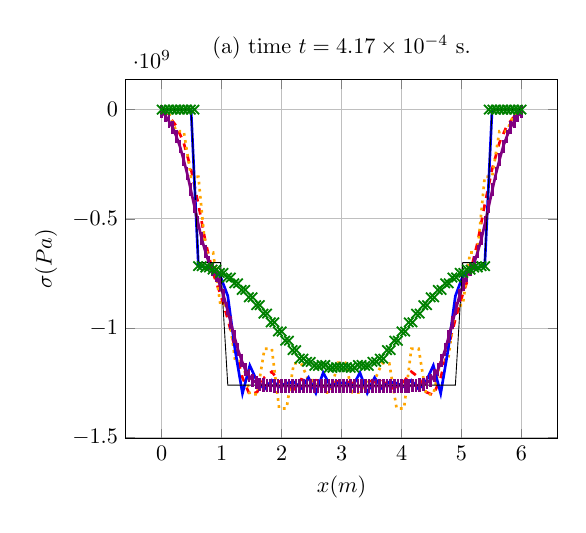
\begin{tikzpicture}[scale=0.8]
\begin{axis}[xlabel=$x (m)$,ylabel=$\sigma (Pa)$,ymajorgrids=true,xmajorgrids=true,legend pos=outer north east,title={(a) time $t = 4.17\times 10^{-4} $ s.}]
\addplot[Red,very thick,mark=none,dashed,mark size=3pt] coordinates {(0.0,-8613486.937425343) (0.12244897959183673,-32098082.523617607) (0.24489795918367346,-75184156.81448549) (0.36734693877551017,-152006982.04059458) (0.4897959183673469,-272918299.7571908) (0.6122448979591837,-434866115.3917057) (0.7346938775510203,-610982765.9130303) (0.8571428571428571,-748144953.2233859) (0.9795918367346939,-845561032.3267925) (1.1020408163265305,-958425749.0711806) (1.2244897959183674,-1093872940.3932045) (1.346938775510204,-1225940785.1464355) (1.4693877551020407,-1306595231.2314239) (1.5918367346938775,-1292395303.4332397) (1.7142857142857142,-1224981707.482427) (1.836734693877551,-1199290066.9091918) (1.9591836734693877,-1243789659.077468) (2.0816326530612246,-1268868931.2157116) (2.204081632653061,-1279555678.011958) (2.326530612244898,-1233843965.2013993) (2.4489795918367347,-1247141973.55301) (2.571428571428571,-1238578154.7331731) (2.693877551020408,-1267018472.19709) (2.816326530612245,-1251288495.1191645) (2.9387755102040813,-1243897445.9598322) (3.061224489795918,-1243897435.653917) (3.183673469387755,-1251288503.290518) (3.306122448979592,-1267018428.6038225) (3.4285714285714284,-1238578260.808024) (3.5510204081632653,-1247141795.020678) (3.673469387755102,-1233843980.264652) (3.7959183673469385,-1279555708.0603902) (3.9183673469387754,-1268868951.8947906) (4.040816326530612,-1243789871.0589092) (4.163265306122449,-1199290088.7219405) (4.285714285714286,-1224981642.7661428) (4.408163265306122,-1292395301.959645) (4.530612244897959,-1306595226.543051) (4.653061224489796,-1225940771.116342) (4.775510204081632,-1093872923.6488597) (4.8979591836734695,-958425734.4341587) (5.020408163265306,-845561024.6840333) (5.142857142857142,-748144947.3854173) (5.26530612244898,-610982760.9679779) (5.387755102040816,-434866113.85137385) (5.5102040816326525,-272918299.19915956) (5.63265306122449,-152006981.87613484) (5.755102040816326,-75184156.77668796) (5.877551020408163,-32098082.517845426) (6.0,-8613486.937112756) };
\addplot[Orange,very thick,mark=none,dotted,mark size=3pt] coordinates {(0.0,-19486450.00530802) (0.12244897959183673,-19486451.37255413) (0.24489795918367346,-98883525.16193365) (0.36734693877551017,-98883532.35877307) (0.4897959183673469,-307042948.5329649) (0.6122448979591837,-307042973.8393218) (0.7346938775510203,-653662753.2107606) (0.8571428571428571,-653662791.3443154) (0.9795918367346939,-895033212.2083819) (1.1020408163265305,-895033210.2294395) (1.2244897959183674,-1149711785.0376468) (1.346938775510204,-1149711707.6439426) (1.4693877551020407,-1302739092.3749402) (1.5918367346938775,-1302739042.5575087) (1.7142857142857142,-1094479333.510092) (1.836734693877551,-1094479363.641839) (1.9591836734693877,-1367729442.0453632) (2.0816326530612246,-1367729367.5886066) (2.204081632653061,-1161379499.150298) (2.326530612244898,-1161379598.2026331) (2.4489795918367347,-1238878624.5589573) (2.571428571428571,-1238878689.4608257) (2.693877551020408,-1294478206.9174366) (2.816326530612245,-1294478350.007934) (2.9387755102040813,-1158113298.5889149) (3.061224489795918,-1158113331.6700864) (3.183673469387755,-1294477877.3735123) (3.306122448979592,-1294477954.2759767) (3.4285714285714284,-1238878389.3714159) (3.5510204081632653,-1238878336.5056608) (3.673469387755102,-1161379397.0010178) (3.7959183673469385,-1161379295.220285) (3.9183673469387754,-1367729506.3247807) (4.040816326530612,-1367729486.415212) (4.163265306122449,-1094479488.8470607) (4.285714285714286,-1094479504.218566) (4.408163265306122,-1302739089.2586887) (4.530612244897959,-1302739090.6284595) (4.653061224489796,-1149711763.4099293) (4.775510204081632,-1149711761.6734378) (4.8979591836734695,-895033202.7697786) (5.020408163265306,-895033202.8404319) (5.142857142857142,-653662748.8713347) (5.26530612244898,-653662750.5779299) (5.387755102040816,-307042947.2123353) (5.5102040816326525,-307042947.98137856) (5.63265306122449,-98883524.96726042) (5.755102040816326,-98883525.08736782) (5.877551020408163,-19486450.128640544) (6.0,-19486450.13761897) };
\addplot[Blue,very thick,mark=none,solid,mark size=3pt] coordinates {(0.0,-6.648826343127885e-07) (0.12244897959183673,4.986619757345916e-07) (0.24489795918367346,-6.648826343127894e-07) (0.36734693877551017,6.648826343127889e-07) (0.4897959183673469,-3.324413171563951e-07) (0.6122448979591837,-715667367.438887) (0.7346938775510203,-721624002.2150931) (0.8571428571428571,-733440346.5979226) (0.9795918367346939,-762779433.8121859) (1.1020408163265305,-852759583.0719095) (1.2244897959183674,-1101085033.4809394) (1.346938775510204,-1298836944.1354702) (1.4693877551020407,-1171100114.2056987) (1.5918367346938775,-1244615764.4304001) (1.7142857142857142,-1279401316.71709) (1.836734693877551,-1238612976.7167482) (1.9591836734693877,-1268822286.952483) (2.0816326530612246,-1251851454.2582784) (2.204081632653061,-1246344358.2784605) (2.326530612244898,-1274636654.590367) (2.4489795918367347,-1226444366.5447345) (2.571428571428571,-1297309357.6096141) (2.693877551020408,-1203729922.9079342) (2.816326530612245,-1267608663.445644) (2.9387755102040813,-1250429639.6986516) (3.061224489795918,-1250429639.698652) (3.183673469387755,-1267608663.4456437) (3.306122448979592,-1203729922.9079332) (3.4285714285714284,-1297309357.6096146) (3.5510204081632653,-1226444366.5447364) (3.673469387755102,-1274636654.5903707) (3.7959183673469385,-1246344358.2784586) (3.9183673469387754,-1251851454.2582788) (4.040816326530612,-1268822286.952483) (4.163265306122449,-1238612976.716749) (4.285714285714286,-1279401316.717093) (4.408163265306122,-1244615764.4303992) (4.530612244897959,-1171100114.205699) (4.653061224489796,-1298836944.1354706) (4.775510204081632,-1101085033.480938) (4.8979591836734695,-852759583.0719106) (5.020408163265306,-762779433.8121861) (5.142857142857142,-733440346.5979232) (5.26530612244898,-721624002.2150935) (5.387755102040816,-715667367.4388872) (5.5102040816326525,6.648826343127891e-07) (5.63265306122449,-8.311032928909869e-07) (5.755102040816326,6.64882634312789e-07) (5.877551020408163,-4.986619757345927e-07) (6.0,6.648826343127891e-07) };
\addplot[Purple,very thick,mark=|,solid,mark size=3pt] coordinates {(0.0,-10102308.696129723) (0.06060606060606061,-27819035.408597022) (0.12121212121212122,-53548174.10156911) (0.18181818181818182,-81220530.91552682) (0.24242424242424243,-121996638.1282555) (0.30303030303030304,-167271442.91399714) (0.36363636363636365,-227374416.8224694) (0.42424242424242425,-291884207.62740797) (0.48484848484848486,-366561331.82425076) (0.5454545454545454,-442651846.10117203) (0.6060606060606061,-517981788.6506681) (0.6666666666666667,-590163308.883224) (0.7272727272727273,-649294423.8320683) (0.7878787878787878,-701741095.1196218) (0.8484848484848485,-730769282.7949975) (0.9090909090909092,-756872056.3761383) (0.9696969696969697,-801569181.7407509) (1.0303030303030303,-849177673.0800432) (1.0909090909090908,-911084939.7727154) (1.1515151515151516,-974214002.7169627) (1.2121212121212122,-1038167680.0536075) (1.2727272727272727,-1099090105.6739883) (1.3333333333333335,-1147307672.5705764) (1.393939393939394,-1190753537.809418) (1.4545454545454546,-1216875899.9474456) (1.5151515151515151,-1239215801.8963046) (1.5757575757575757,-1249066695.0125978) (1.6363636363636365,-1257474117.1450398) (1.696969696969697,-1260287231.5732214) (1.7575757575757576,-1262882155.5942452) (1.8181818181818183,-1263639434.435723) (1.878787878787879,-1264451227.6039906) (1.9393939393939394,-1264700974.3286438) (2.0,-1264995274.0914948) (2.0606060606060606,-1265081753.3010664) (2.121212121212121,-1265196971.579899) (2.1818181818181817,-1265214637.004615) (2.2424242424242427,-1265254598.958957) (2.303030303030303,-1265245140.1058884) (2.3636363636363638,-1265256293.5490305) (2.4242424242424243,-1265242505.3887954) (2.484848484848485,-1265248286.884651) (2.5454545454545454,-1265240360.2874153) (2.606060606060606,-1265250508.029845) (2.666666666666667,-1265248914.1312644) (2.7272727272727275,-1265263548.0936751) (2.787878787878788,-1265262744.314047) (2.8484848484848486,-1265286671.3434186) (2.909090909090909,-1265283781.3906841) (2.9696969696969697,-1265290450.4639096) (3.0303030303030303,-1265290450.4639094) (3.090909090909091,-1265283781.3906841) (3.1515151515151514,-1265286671.3434184) (3.2121212121212124,-1265262744.3140473) (3.272727272727273,-1265263548.0936751) (3.3333333333333335,-1265248914.1312644) (3.393939393939394,-1265250508.029845) (3.4545454545454546,-1265240360.2874155) (3.515151515151515,-1265248286.884651) (3.5757575757575757,-1265242505.3887959) (3.6363636363636367,-1265256293.5490305) (3.6969696969696972,-1265245140.1058888) (3.757575757575758,-1265254598.9589574) (3.8181818181818183,-1265214637.0046158) (3.878787878787879,-1265196971.5798993) (3.9393939393939394,-1265081753.301067) (4.0,-1264995274.0914955) (4.0606060606060606,-1264700974.3286445) (4.121212121212121,-1264451227.603991) (4.181818181818182,-1263639434.4357235) (4.242424242424242,-1262882155.5942454) (4.303030303030303,-1260287231.5732222) (4.363636363636363,-1257474117.1450403) (4.424242424242425,-1249066695.0125985) (4.484848484848485,-1239215801.896305) (4.545454545454546,-1216875899.9474466) (4.606060606060606,-1190753537.8094187) (4.666666666666667,-1147307672.5705774) (4.7272727272727275,-1099090105.6739895) (4.787878787878788,-1038167680.053609) (4.848484848484849,-974214002.7169627) (4.909090909090909,-911084939.772716) (4.96969696969697,-849177673.0800438) (5.03030303030303,-801569181.7407513) (5.090909090909091,-756872056.3761387) (5.151515151515151,-730769282.7949976) (5.212121212121212,-701741095.1196221) (5.2727272727272725,-649294423.8320689) (5.333333333333334,-590163308.8832242) (5.3939393939393945,-517981788.6506686) (5.454545454545455,-442651846.10117245) (5.515151515151516,-366561331.82425123) (5.575757575757576,-291884207.62740815) (5.636363636363637,-227374416.82246974) (5.696969696969697,-167271442.91399717) (5.757575757575758,-121996638.12825578) (5.818181818181818,-81220530.91552722) (5.878787878787879,-53548174.101569325) (5.9393939393939394,-27819035.408597216) (6.0,-10102308.696129855) };
\addplot[Green,thick,mark=x,only marks,mark size=3pt] coordinates {(0.0,-2.0877147917780336e-07) (0.06060606060606061,-1.23669837978591e-07) (0.12121212121212122,1.0131895444177197e-06) (0.18181818181818182,9.814583585206487e-07) (0.24242424242424243,-5.619879278457838e-07) (0.30303030303030304,-7.677773407797948e-07) (0.36363636363636365,4.815476698956227e-07) (0.42424242424242425,1.8333496441716677e-07) (0.48484848484848486,1.0440135561077701e-07) (0.5454545454545454,2.2803996154561766e-07) (0.6060606060606061,-716376930.5893724) (0.6666666666666667,-716376930.589367) (0.7272727272727273,-722477457.3590242) (0.7878787878787878,-722477457.3590261) (0.8484848484848485,-732178472.6355962) (0.9090909090909092,-732178472.6355944) (0.9696969696969697,-747351730.2863077) (1.0303030303030303,-747351730.2863119) (1.0909090909090908,-768562816.0383832) (1.1515151515151516,-768562816.0383828) (1.2121212121212122,-794945415.8744416) (1.2727272727272727,-794945415.8744432) (1.3333333333333335,-825275759.4899069) (1.393939393939394,-825275759.4899055) (1.4545454545454546,-858914148.2093647) (1.5151515151515151,-858914148.2093657) (1.5757575757575757,-895001130.8125886) (1.6363636363636365,-895001130.8125875) (1.696969696969697,-933584126.6213479) (1.7575757575757576,-933584126.6213498) (1.8181818181818183,-973568810.43142) (1.878787878787879,-973568810.4314172) (1.9393939393939394,-1015496794.5721984) (2.0,-1015496794.57219) (2.0606060606060606,-1057685588.3287526) (2.121212121212121,-1057685588.3287554) (2.1818181818181817,-1100692545.9682453) (2.2424242424242427,-1100692545.968236) (2.303030303030303,-1139792908.6344922) (2.3636363636363638,-1139792908.6344938) (2.4242424242424243,-1154354135.2303133) (2.484848484848485,-1154354135.2299874) (2.5454545454545454,-1172832255.3077557) (2.606060606060606,-1172832255.3077602) (2.666666666666667,-1168855409.3584068) (2.7272727272727275,-1168855409.358407) (2.787878787878788,-1181372468.846199) (2.8484848484848486,-1181372468.8461988) (2.909090909090909,-1178905236.4784043) (2.9696969696969697,-1178905236.4784184) (3.0303030303030303,-1178905236.4783716) (3.090909090909091,-1178905236.4783936) (3.1515151515151514,-1181372468.8462052) (3.2121212121212124,-1181372468.8462112) (3.272727272727273,-1168855409.3585627) (3.3333333333333335,-1168855409.3585649) (3.393939393939394,-1172832255.307782) (3.4545454545454546,-1172832255.3077602) (3.515151515151515,-1154354135.2301552) (3.5757575757575757,-1154354135.2301497) (3.6363636363636367,-1139792908.6344705) (3.6969696969696972,-1139792908.6344807) (3.757575757575758,-1100692545.9682417) (3.8181818181818183,-1100692545.968244) (3.878787878787879,-1057685588.3287588) (3.9393939393939394,-1057685588.3287547) (4.0,-1015496794.572189) (4.0606060606060606,-1015496794.5721911) (4.121212121212121,-973568810.4314169) (4.181818181818182,-973568810.4314196) (4.242424242424242,-933584126.6213472) (4.303030303030303,-933584126.6213481) (4.363636363636363,-895001130.8125902) (4.424242424242425,-895001130.8125896) (4.484848484848485,-858914148.2093651) (4.545454545454546,-858914148.2093666) (4.606060606060606,-825275759.4899112) (4.666666666666667,-825275759.4899105) (4.7272727272727275,-794945415.8744518) (4.787878787878788,-794945415.8744564) (4.848484848484849,-768562816.0383911) (4.909090909090909,-768562816.0383939) (4.96969696969697,-747351730.286324) (5.03030303030303,-747351730.2863271) (5.090909090909091,-732178472.6356105) (5.151515151515151,-732178472.6356128) (5.212121212121212,-722477457.3590274) (5.2727272727272725,-722477457.3590299) (5.333333333333334,-716376930.5893677) (5.3939393939393945,-716376930.5893692) (5.454545454545455,6.698192810303248e-07) (5.515151515151516,6.599459875952535e-07) (5.575757575757576,-9.369788715662316e-07) (5.636363636363637,-1.0576690313721361e-06) (5.696969696969697,1.675441116120912e-06) (5.757575757575758,1.6489720554430353e-06) (5.818181818181818,-1.0608989471845062e-06) (5.878787878787879,-9.337489557538617e-07) (5.9393939393939394,1.4751713795395358e-06) (6.0,1.5168004748680168e-06) };
\addplot[black,thin,mark=none,solid,mark size=3pt] coordinates {(0.0,-0.0) (0.12244897959183673,-0.0) (0.24489795918367346,-0.0) (0.36734693877551017,-0.0) (0.4897959183673469,-0.0) (0.6122448979591837,-700000000.0) (0.7346938775510203,-700000000.0) (0.8571428571428571,-700000000.0) (0.9795918367346939,-700000000.0) (1.1020408163265305,-1261004576.260559) (1.2244897959183674,-1261004576.260559) (1.346938775510204,-1261004576.260559) (1.4693877551020407,-1261004576.260559) (1.5918367346938775,-1261004576.260559) (1.7142857142857142,-1261004576.260559) (1.836734693877551,-1261004576.260559) (1.9591836734693877,-1261004576.260559) (2.0816326530612246,-1261004576.260559) (2.204081632653061,-1261004576.260559) (2.326530612244898,-1261004576.260559) (2.4489795918367347,-1261004576.260559) (2.571428571428571,-1261004576.260559) (2.693877551020408,-1261004576.260559) (2.816326530612245,-1261004576.260559) (2.9387755102040813,-1261004576.260559) (3.061224489795918,-1261004576.260559) (3.183673469387755,-1261004576.260559) (3.306122448979592,-1261004576.260559) (3.4285714285714284,-1261004576.260559) (3.5510204081632653,-1261004576.260559) (3.673469387755102,-1261004576.260559) (3.7959183673469385,-1261004576.260559) (3.9183673469387754,-1261004576.260559) (4.040816326530612,-1261004576.260559) (4.163265306122449,-1261004576.260559) (4.285714285714286,-1261004576.260559) (4.408163265306122,-1261004576.260559) (4.530612244897959,-1261004576.260559) (4.653061224489796,-1261004576.260559) (4.775510204081632,-1261004576.260559) (4.8979591836734695,-1261004576.260559) (5.020408163265306,-700000000.0) (5.142857142857142,-700000000.0) (5.26530612244898,-700000000.0) (5.387755102040816,-700000000.0) (5.5102040816326525,-0.0) (5.63265306122449,-0.0) (5.755102040816326,-0.0) (5.877551020408163,-0.0) (6.0,-0.0) };
%\legend{usl 1ppc,usf 1ppc,dgmpm 1ppc,dgmpm 2ppc,dgmpm 2ppc (RK2 + strang),plastic solution}
\end{axis}
\end{tikzpicture}
%%% Local Variables:
%%% mode: latex
%%% TeX-master: "../../mainManuscript"
%%% End:
}
  % {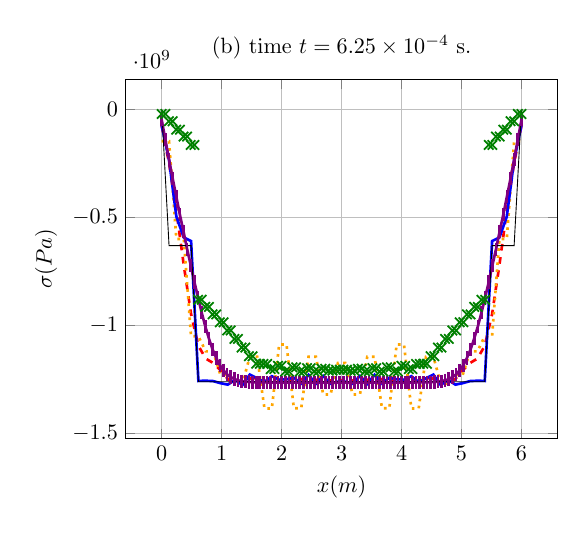
\begin{tikzpicture}[scale=0.8]
\begin{axis}[xlabel=$x (m)$,ylabel=$\sigma (Pa)$,ymajorgrids=true,xmajorgrids=true,legend pos=outer north east,title={(b) time $t = 6.25\times 10^{-4} $ s.}]
\addplot[Red,very thick,mark=none,dashed,mark size=3pt] coordinates {(0.0,-74755364.74533166) (0.12244897959183673,-248208896.12486583) (0.24489795918367346,-468625717.803481) (0.36734693877551017,-719013533.7365903) (0.4897959183673469,-947742026.6398356) (0.6122448979591837,-1094792437.4560761) (0.7346938775510203,-1153839566.2578583) (0.8571428571428571,-1174113393.2907) (0.9795918367346939,-1207454154.8556237) (1.1020408163265305,-1248053189.0341141) (1.2244897959183674,-1269531290.7275531) (1.346938775510204,-1257538829.8363345) (1.4693877551020407,-1246174055.5311027) (1.5918367346938775,-1243899733.863632) (1.7142857142857142,-1257815798.8450537) (1.836734693877551,-1259247134.6249063) (1.9591836734693877,-1263208926.5266936) (2.0816326530612246,-1248288130.419574) (2.204081632653061,-1261500638.8122087) (2.326530612244898,-1248516389.0385368) (2.4489795918367347,-1265795229.6578722) (2.571428571428571,-1251562844.0674527) (2.693877551020408,-1262749976.8464308) (2.816326530612245,-1255375541.0724187) (2.9387755102040813,-1253751855.6811213) (3.061224489795918,-1253751839.0824046) (3.183673469387755,-1255375534.8022113) (3.306122448979592,-1262749921.7411852) (3.4285714285714284,-1251562950.169376) (3.5510204081632653,-1265795057.7459216) (3.673469387755102,-1248516391.9733808) (3.7959183673469385,-1261500630.050308) (3.9183673469387754,-1248288097.1119542) (4.040816326530612,-1263209080.4260836) (4.163265306122449,-1259247117.6459212) (4.285714285714286,-1257815707.7658777) (4.408163265306122,-1243899712.3822339) (4.530612244897959,-1246174035.7380946) (4.653061224489796,-1257539140.237503) (4.775510204081632,-1269531234.7005646) (4.8979591836734695,-1248053690.7012877) (5.020408163265306,-1207453700.9419231) (5.142857142857142,-1174113502.2223024) (5.26530612244898,-1153838796.8971734) (5.387755102040816,-1094792530.955986) (5.5102040816326525,-947741675.2773904) (5.63265306122449,-719013481.172835) (5.755102040816326,-468625706.5592639) (5.877551020408163,-248208829.82757288) (6.0,-74755344.97904286) };
\addplot[Orange,very thick,mark=none,dotted,mark size=3pt] coordinates {(0.0,-146910686.54340002) (0.12244897959183673,-146910576.6778985) (0.24489795918367346,-599499161.4545292) (0.36734693877551017,-599499345.0291598) (0.4897959183673469,-1050556946.940909) (0.6122448979591837,-1050556810.8531282) (0.7346938775510203,-1120414463.9040096) (0.8571428571428571,-1120414507.6770024) (0.9795918367346939,-1229455185.2009192) (1.1020408163265305,-1229455106.2082894) (1.2244897959183674,-1269042253.7721956) (1.346938775510204,-1269042214.6789474) (1.4693877551020407,-1144813454.0089188) (1.5918367346938775,-1144813966.490456) (1.7142857142857142,-1385034660.973245) (1.836734693877551,-1385034240.6909063) (1.9591836734693877,-1088744428.4000087) (2.0816326530612246,-1088744356.7882442) (2.204081632653061,-1383996748.4707298) (2.326530612244898,-1383996722.000206) (2.4489795918367347,-1144999088.7730293) (2.571428571428571,-1144998814.9657073) (2.693877551020408,-1320236218.1167607) (2.816326530612245,-1320236958.4771528) (2.9387755102040813,-1174522093.1728597) (3.061224489795918,-1174521439.5484982) (3.183673469387755,-1320235859.9132228) (3.306122448979592,-1320235657.2910552) (3.4285714285714284,-1145000190.5115752) (3.5510204081632653,-1144999698.2190187) (3.673469387755102,-1383996750.799452) (3.7959183673469385,-1383996409.8226683) (3.9183673469387754,-1088744644.3503904) (4.040816326530612,-1088744177.3418117) (4.163265306122449,-1385034239.357628) (4.285714285714286,-1385034463.0774357) (4.408163265306122,-1144813430.515698) (4.530612244897959,-1144813914.0897422) (4.653061224489796,-1269041947.1103678) (4.775510204081632,-1269041892.7174592) (4.8979591836734695,-1229455306.2104805) (5.020408163265306,-1229455419.0438316) (5.142857142857142,-1120414629.727034) (5.26530612244898,-1120414606.2420225) (5.387755102040816,-1050556872.9115263) (5.5102040816326525,-1050556814.2558659) (5.63265306122449,-599499269.4389613) (5.755102040816326,-599499363.047376) (5.877551020408163,-146910684.6411048) (6.0,-146910614.3275735) };
\addplot[Blue,very thick,mark=none,solid,mark size=3pt] coordinates {(0.0,-73372434.82033628) (0.12244897959183673,-233858719.55212942) (0.24489795918367346,-495938295.48681855) (0.36734693877551017,-592504781.1553047) (0.4897959183673469,-609199055.9406189) (0.6122448979591837,-1257272451.0662038) (0.7346938775510203,-1256464300.2954264) (0.8571428571428571,-1258068523.1986136) (0.9795918367346939,-1267655174.0427077) (1.1020408163265305,-1274486401.3694665) (1.2244897959183674,-1252604107.07487) (1.346938775510204,-1276531816.9026763) (1.4693877551020407,-1227937227.7003279) (1.5918367346938775,-1245313491.0436618) (1.7142857142857142,-1262325040.1928196) (1.836734693877551,-1235608282.656636) (1.9591836734693877,-1251386670.8684802) (2.0816326530612246,-1249617525.1753566) (2.204081632653061,-1242442736.3652022) (2.326530612244898,-1269356567.5147986) (2.4489795918367347,-1229053885.1472373) (2.571428571428571,-1271114130.25009) (2.693877551020408,-1234588132.0907624) (2.816326530612245,-1270149960.4084883) (2.9387755102040813,-1260862894.9637291) (3.061224489795918,-1260862894.963727) (3.183673469387755,-1270149960.4084873) (3.306122448979592,-1234588132.0907636) (3.4285714285714284,-1271114130.2500923) (3.5510204081632653,-1229053885.1472325) (3.673469387755102,-1269356567.5148) (3.7959183673469385,-1242442736.3652017) (3.9183673469387754,-1249617525.1753573) (4.040816326530612,-1251386670.8684816) (4.163265306122449,-1235608282.6566362) (4.285714285714286,-1262325040.1928182) (4.408163265306122,-1245313491.0436635) (4.530612244897959,-1227937227.7003253) (4.653061224489796,-1276531816.9026778) (4.775510204081632,-1252604107.074872) (4.8979591836734695,-1274486401.3694673) (5.020408163265306,-1267655174.0427058) (5.142857142857142,-1258068523.1986136) (5.26530612244898,-1256464300.2954257) (5.387755102040816,-1257272451.0662048) (5.5102040816326525,-609199055.940622) (5.63265306122449,-592504781.1553006) (5.755102040816326,-495938295.48681825) (5.877551020408163,-233858719.55212817) (6.0,-73372434.82033731) };
\addplot[Purple,very thick,mark=|,solid,mark size=3pt] coordinates {(0.0,-47333356.22779358) (0.06060606060606061,-138756545.0597926) (0.12121212121212122,-229985791.05287215) (0.18181818181818182,-318140237.4578) (0.24242424242424243,-402202061.10697633) (0.30303030303030304,-486791312.40641415) (0.36363636363636365,-564994266.2878431) (0.42424242424242425,-646698716.5243026) (0.48484848484848486,-721593111.9376383) (0.5454545454545454,-799220239.6164875) (0.6060606060606061,-870833555.6318947) (0.6666666666666667,-940547799.3769101) (0.7272727272727273,-1004764341.06167) (0.7878787878787878,-1060903097.5027591) (0.8484848484848485,-1111526011.847744) (0.9090909090909092,-1150516460.50863) (0.9696969696969697,-1184534064.1013935) (1.0303030303030303,-1207708133.016495) (1.0909090909090908,-1227220308.6256344) (1.1515151515151516,-1239136300.842325) (1.2121212121212122,-1248834908.9252155) (1.2727272727272727,-1254207515.376704) (1.3333333333333335,-1258429252.1271956) (1.393939393939394,-1260585212.884834) (1.4545454545454546,-1262234236.0930166) (1.5151515151515151,-1263047159.404436) (1.5757575757575757,-1263653386.8297281) (1.6363636363636365,-1263951357.5622544) (1.696969696969697,-1264163825.8617294) (1.7575757575757576,-1264271933.08496) (1.8181818181818183,-1264341903.226051) (1.878787878787879,-1264380965.5508432) (1.9393939393939394,-1264400307.6802652) (2.0,-1264413367.7497914) (2.0606060606060606,-1264414399.1473076) (2.121212121212121,-1264416892.3074598) (2.1818181818181817,-1264411289.2771008) (2.2424242424242427,-1264409453.8903484) (2.303030303030303,-1264402104.3991406) (2.3636363636363638,-1264399159.0796075) (2.4242424242424243,-1264392461.8213086) (2.484848484848485,-1264390501.27199) (2.5454545454545454,-1264385501.2848275) (2.606060606060606,-1264385712.5692852) (2.666666666666667,-1264382271.7032228) (2.7272727272727275,-1264384650.233929) (2.787878787878788,-1264381389.2284317) (2.8484848484848486,-1264388956.0046396) (2.909090909090909,-1264385898.768779) (2.9696969696969697,-1264387667.9110923) (3.0303030303030303,-1264387667.911092) (3.090909090909091,-1264385898.768779) (3.1515151515151514,-1264388956.0046391) (3.2121212121212124,-1264381389.2284312) (3.272727272727273,-1264384650.2339287) (3.3333333333333335,-1264382271.7032225) (3.393939393939394,-1264385712.569285) (3.4545454545454546,-1264385501.2848277) (3.515151515151515,-1264390501.2719903) (3.5757575757575757,-1264392461.8213089) (3.6363636363636367,-1264399159.0796077) (3.6969696969696972,-1264402104.399141) (3.757575757575758,-1264409453.8903487) (3.8181818181818183,-1264411289.277101) (3.878787878787879,-1264416892.30746) (3.9393939393939394,-1264414399.1473076) (4.0,-1264413367.7497916) (4.0606060606060606,-1264400307.6802652) (4.121212121212121,-1264380965.5508432) (4.181818181818182,-1264341903.2260516) (4.242424242424242,-1264271933.0849605) (4.303030303030303,-1264163825.8617299) (4.363636363636363,-1263951357.5622554) (4.424242424242425,-1263653386.8297288) (4.484848484848485,-1263047159.4044366) (4.545454545454546,-1262234236.093017) (4.606060606060606,-1260585212.8848348) (4.666666666666667,-1258429252.127196) (4.7272727272727275,-1254207515.3767045) (4.787878787878788,-1248834908.925216) (4.848484848484849,-1239136300.8423254) (4.909090909090909,-1227220308.6256351) (4.96969696969697,-1207708133.0164952) (5.03030303030303,-1184534064.1013935) (5.090909090909091,-1150516460.50863) (5.151515151515151,-1111526011.847744) (5.212121212121212,-1060903097.5027591) (5.2727272727272725,-1004764341.0616697) (5.333333333333334,-940547799.3769101) (5.3939393939393945,-870833555.6318948) (5.454545454545455,-799220239.6164877) (5.515151515151516,-721593111.9376383) (5.575757575757576,-646698716.5243028) (5.636363636363637,-564994266.2878435) (5.696969696969697,-486791312.4064143) (5.757575757575758,-402202061.1069768) (5.818181818181818,-318140237.4578002) (5.878787878787879,-229985791.0528724) (5.9393939393939394,-138756545.05979264) (6.0,-47333356.22779366) };
\addplot[Green,thick,mark=x,only marks,mark size=3pt] coordinates {(0.0,-20229275.520624813) (0.06060606060606061,-20229275.520624828) (0.12121212121212122,-53902709.192570105) (0.18181818181818182,-53902709.192569956) (0.24242424242424243,-93046882.15578794) (0.30303030303030304,-93046882.1557879) (0.36363636363636365,-124818495.63572057) (0.42424242424242425,-124818495.6357201) (0.48484848484848486,-163811216.3609897) (0.5454545454545454,-163811216.36098817) (0.6060606060606061,-881303240.5770407) (0.6666666666666667,-881303240.5770347) (0.7272727272727273,-914303290.6106135) (0.7878787878787878,-914303290.610614) (0.8484848484848485,-949108866.3150425) (0.9090909090909092,-949108866.3150418) (0.9696969696969697,-985587474.2698758) (1.0303030303030303,-985587474.2698789) (1.0909090909090908,-1023460684.7529197) (1.1515151515151516,-1023460684.7529227) (1.2121212121212122,-1062676463.9811376) (1.2727272727272727,-1062676463.9811432) (1.3333333333333335,-1102710418.5537071) (1.393939393939394,-1102710418.553707) (1.4545454545454546,-1142958071.2150478) (1.5151515151515151,-1142958071.2150497) (1.5757575757575757,-1177713108.448572) (1.6363636363636365,-1177713108.4485712) (1.696969696969697,-1178607832.5129364) (1.7575757575757576,-1178607832.5129366) (1.8181818181818183,-1202493123.9660535) (1.878787878787879,-1202493123.966045) (1.9393939393939394,-1187462459.6258917) (2.0,-1187462459.6258917) (2.0606060606060606,-1213334125.432626) (2.121212121212121,-1213334125.4325962) (2.1818181818181817,-1194303471.3523695) (2.2424242424242427,-1194303471.35237) (2.303030303030303,-1213800467.2016068) (2.3636363636363638,-1213800467.201615) (2.4242424242424243,-1198169738.036603) (2.484848484848485,-1198169738.036608) (2.5454545454545454,-1213000678.5547864) (2.606060606060606,-1213000678.5547855) (2.666666666666667,-1201083468.1228912) (2.7272727272727275,-1201083468.122941) (2.787878787878788,-1210046074.450863) (2.8484848484848486,-1210046074.4508822) (2.909090909090909,-1205397510.3980381) (2.9696969696969697,-1205397510.3980904) (3.0303030303030303,-1205397510.3980312) (3.090909090909091,-1205397510.3980837) (3.1515151515151514,-1210046074.4509275) (3.2121212121212124,-1210046074.450946) (3.272727272727273,-1201083468.122753) (3.3333333333333335,-1201083468.1228034) (3.393939393939394,-1213000678.5547462) (3.4545454545454546,-1213000678.5547454) (3.515151515151515,-1198169738.0364976) (3.5757575757575757,-1198169738.0364983) (3.6363636363636367,-1213800467.20157) (3.6969696969696972,-1213800467.2015686) (3.757575757575758,-1194303471.3523912) (3.8181818181818183,-1194303471.3523917) (3.878787878787879,-1213334125.432576) (3.9393939393939394,-1213334125.432606) (4.0,-1187462459.6258657) (4.0606060606060606,-1187462459.625866) (4.121212121212121,-1202493123.966091) (4.181818181818182,-1202493123.966098) (4.242424242424242,-1178607832.513093) (4.303030303030303,-1178607832.5130925) (4.363636363636363,-1177713108.448581) (4.424242424242425,-1177713108.4485826) (4.484848484848485,-1142958071.215055) (4.545454545454546,-1142958071.2150486) (4.606060606060606,-1102710418.5537033) (4.666666666666667,-1102710418.5537047) (4.7272727272727275,-1062676463.9811467) (4.787878787878788,-1062676463.9811449) (4.848484848484849,-1023460684.7529202) (4.909090909090909,-1023460684.7529212) (4.96969696969697,-985587474.2698778) (5.03030303030303,-985587474.2698749) (5.090909090909091,-949108866.315046) (5.151515151515151,-949108866.3150446) (5.212121212121212,-914303290.6106138) (5.2727272727272725,-914303290.6106144) (5.333333333333334,-881303240.5770384) (5.3939393939393945,-881303240.5770377) (5.454545454545455,-163811216.3609834) (5.515151515151516,-163811216.3609822) (5.575757575757576,-124818495.63570935) (5.636363636363637,-124818495.63570964) (5.696969696969697,-93046882.15578243) (5.757575757575758,-93046882.15578227) (5.818181818181818,-53902709.192592174) (5.878787878787879,-53902709.19259214) (5.9393939393939394,-20229275.520634342) (6.0,-20229275.520634633) };
\addplot[black,thin,mark=none,solid,mark size=3pt] coordinates {(0.0,-0.0) (0.12244897959183673,-630502288.1302795) (0.24489795918367346,-630502288.1302795) (0.36734693877551017,-630502288.1302795) (0.4897959183673469,-630502288.1302795) (0.6122448979591837,-1261004576.260559) (0.7346938775510203,-1261004576.260559) (0.8571428571428571,-1261004576.260559) (0.9795918367346939,-1261004576.260559) (1.1020408163265305,-1261004576.260559) (1.2244897959183674,-1261004576.260559) (1.346938775510204,-1261004576.260559) (1.4693877551020407,-1261004576.260559) (1.5918367346938775,-1261004576.260559) (1.7142857142857142,-1261004576.260559) (1.836734693877551,-1261004576.260559) (1.9591836734693877,-1261004576.260559) (2.0816326530612246,-1261004576.260559) (2.204081632653061,-1261004576.260559) (2.326530612244898,-1261004576.260559) (2.4489795918367347,-1261004576.260559) (2.571428571428571,-1261004576.260559) (2.693877551020408,-1261004576.260559) (2.816326530612245,-1261004576.260559) (2.9387755102040813,-1261004576.260559) (3.061224489795918,-1261004576.260559) (3.183673469387755,-1261004576.260559) (3.306122448979592,-1261004576.260559) (3.4285714285714284,-1261004576.260559) (3.5510204081632653,-1261004576.260559) (3.673469387755102,-1261004576.260559) (3.7959183673469385,-1261004576.260559) (3.9183673469387754,-1261004576.260559) (4.040816326530612,-1261004576.260559) (4.163265306122449,-1261004576.260559) (4.285714285714286,-1261004576.260559) (4.408163265306122,-1261004576.260559) (4.530612244897959,-1261004576.260559) (4.653061224489796,-1261004576.260559) (4.775510204081632,-1261004576.260559) (4.8979591836734695,-1261004576.260559) (5.020408163265306,-1261004576.260559) (5.142857142857142,-1261004576.260559) (5.26530612244898,-1261004576.260559) (5.387755102040816,-1261004576.260559) (5.5102040816326525,-630502288.1302795) (5.63265306122449,-630502288.1302795) (5.755102040816326,-630502288.1302795) (5.877551020408163,-630502288.1302795) (6.0,-0.0) };
%\legend{usl 1ppc,usf 1ppc,dgmpm 1ppc,dgmpm 2ppc,dgmpm 2ppc (RK2 + strang),plastic solution}
\end{axis}
\end{tikzpicture}
%%% Local Variables:
%%% mode: latex
%%% TeX-master: "../../mainManuscript"
%%% End:
}
  {\begin{tikzpicture}[scale=.9]
\begin{groupplot}[group style={group size=3 by 2,
ylabels at=edge left, yticklabels at=edge left,horizontal sep=2.ex,
vertical sep=4ex,xticklabels at=edge bottom,xlabels at=edge bottom},
ymajorgrids=true,xmajorgrids=true,enlargelimits=0,xmin=0.,xmax=6.,xlabel=$x (m)$,
axis on top,scale only axis,width=0.32\linewidth
]
\nextgroupplot[title={(a) $t = 4.17\times 10^{-4} $ s.},ymin=-1523538127.0705695,ymax=87935356.1634356,]
\addplot[Red,dashed,mark=none,very thick,mark size=3pt,mark repeat=2] coordinates{(0.0,-8613486.937425343) (0.12244897959183673,-32098082.523617607) (0.24489795918367346,-75184156.81448549) (0.36734693877551017,-152006982.04059458) (0.4897959183673469,-272918299.7571908) (0.6122448979591837,-434866115.3917057) (0.7346938775510203,-610982765.9130303) (0.8571428571428571,-748144953.2233859) (0.9795918367346939,-845561032.3267925) (1.1020408163265305,-958425749.0711806) (1.2244897959183674,-1093872940.3932045) (1.346938775510204,-1225940785.1464355) (1.4693877551020407,-1306595231.2314239) (1.5918367346938775,-1292395303.4332397) (1.7142857142857142,-1224981707.482427) (1.836734693877551,-1199290066.9091918) (1.9591836734693877,-1243789659.077468) (2.0816326530612246,-1268868931.2157116) (2.204081632653061,-1279555678.011958) (2.326530612244898,-1233843965.2013993) (2.4489795918367347,-1247141973.55301) (2.571428571428571,-1238578154.7331731) (2.693877551020408,-1267018472.19709) (2.816326530612245,-1251288495.1191645) (2.9387755102040813,-1243897445.9598322) (3.061224489795918,-1243897435.653917) (3.183673469387755,-1251288503.290518) (3.306122448979592,-1267018428.6038225) (3.4285714285714284,-1238578260.808024) (3.5510204081632653,-1247141795.020678) (3.673469387755102,-1233843980.264652) (3.7959183673469385,-1279555708.0603902) (3.9183673469387754,-1268868951.8947906) (4.040816326530612,-1243789871.0589092) (4.163265306122449,-1199290088.7219405) (4.285714285714286,-1224981642.7661428) (4.408163265306122,-1292395301.959645) (4.530612244897959,-1306595226.543051) (4.653061224489796,-1225940771.116342) (4.775510204081632,-1093872923.6488597) (4.8979591836734695,-958425734.4341587) (5.020408163265306,-845561024.6840333) (5.142857142857142,-748144947.3854173) (5.26530612244898,-610982760.9679779) (5.387755102040816,-434866113.85137385) (5.5102040816326525,-272918299.19915956) (5.63265306122449,-152006981.87613484) (5.755102040816326,-75184156.77668796) (5.877551020408163,-32098082.517845426) (6.0,-8613486.937112756) };
\addplot[Orange,dotted,mark=none,very thick,mark size=3pt,mark repeat=2] coordinates{(0.0,-19486450.00530802) (0.12244897959183673,-19486451.37255413) (0.24489795918367346,-98883525.16193365) (0.36734693877551017,-98883532.35877307) (0.4897959183673469,-307042948.5329649) (0.6122448979591837,-307042973.8393218) (0.7346938775510203,-653662753.2107606) (0.8571428571428571,-653662791.3443154) (0.9795918367346939,-895033212.2083819) (1.1020408163265305,-895033210.2294395) (1.2244897959183674,-1149711785.0376468) (1.346938775510204,-1149711707.6439426) (1.4693877551020407,-1302739092.3749402) (1.5918367346938775,-1302739042.5575087) (1.7142857142857142,-1094479333.510092) (1.836734693877551,-1094479363.641839) (1.9591836734693877,-1367729442.0453632) (2.0816326530612246,-1367729367.5886066) (2.204081632653061,-1161379499.150298) (2.326530612244898,-1161379598.2026331) (2.4489795918367347,-1238878624.5589573) (2.571428571428571,-1238878689.4608257) (2.693877551020408,-1294478206.9174366) (2.816326530612245,-1294478350.007934) (2.9387755102040813,-1158113298.5889149) (3.061224489795918,-1158113331.6700864) (3.183673469387755,-1294477877.3735123) (3.306122448979592,-1294477954.2759767) (3.4285714285714284,-1238878389.3714159) (3.5510204081632653,-1238878336.5056608) (3.673469387755102,-1161379397.0010178) (3.7959183673469385,-1161379295.220285) (3.9183673469387754,-1367729506.3247807) (4.040816326530612,-1367729486.415212) (4.163265306122449,-1094479488.8470607) (4.285714285714286,-1094479504.218566) (4.408163265306122,-1302739089.2586887) (4.530612244897959,-1302739090.6284595) (4.653061224489796,-1149711763.4099293) (4.775510204081632,-1149711761.6734378) (4.8979591836734695,-895033202.7697786) (5.020408163265306,-895033202.8404319) (5.142857142857142,-653662748.8713347) (5.26530612244898,-653662750.5779299) (5.387755102040816,-307042947.2123353) (5.5102040816326525,-307042947.98137856) (5.63265306122449,-98883524.96726042) (5.755102040816326,-98883525.08736782) (5.877551020408163,-19486450.128640544) (6.0,-19486450.13761897) };
\addplot[Blue,solid,mark=none,very thick,mark size=3pt,mark repeat=2] coordinates{(0.0,-6.648826343127885e-07) (0.12244897959183673,4.986619757345916e-07) (0.24489795918367346,-6.648826343127894e-07) (0.36734693877551017,6.648826343127889e-07) (0.4897959183673469,-3.324413171563951e-07) (0.6122448979591837,-715667367.438887) (0.7346938775510203,-721624002.2150931) (0.8571428571428571,-733440346.5979226) (0.9795918367346939,-762779433.8121859) (1.1020408163265305,-852759583.0719095) (1.2244897959183674,-1101085033.4809394) (1.346938775510204,-1298836944.1354702) (1.4693877551020407,-1171100114.2056987) (1.5918367346938775,-1244615764.4304001) (1.7142857142857142,-1279401316.71709) (1.836734693877551,-1238612976.7167482) (1.9591836734693877,-1268822286.952483) (2.0816326530612246,-1251851454.2582784) (2.204081632653061,-1246344358.2784605) (2.326530612244898,-1274636654.590367) (2.4489795918367347,-1226444366.5447345) (2.571428571428571,-1297309357.6096141) (2.693877551020408,-1203729922.9079342) (2.816326530612245,-1267608663.445644) (2.9387755102040813,-1250429639.6986516) (3.061224489795918,-1250429639.698652) (3.183673469387755,-1267608663.4456437) (3.306122448979592,-1203729922.9079332) (3.4285714285714284,-1297309357.6096146) (3.5510204081632653,-1226444366.5447364) (3.673469387755102,-1274636654.5903707) (3.7959183673469385,-1246344358.2784586) (3.9183673469387754,-1251851454.2582788) (4.040816326530612,-1268822286.952483) (4.163265306122449,-1238612976.716749) (4.285714285714286,-1279401316.717093) (4.408163265306122,-1244615764.4303992) (4.530612244897959,-1171100114.205699) (4.653061224489796,-1298836944.1354706) (4.775510204081632,-1101085033.480938) (4.8979591836734695,-852759583.0719106) (5.020408163265306,-762779433.8121861) (5.142857142857142,-733440346.5979232) (5.26530612244898,-721624002.2150935) (5.387755102040816,-715667367.4388872) (5.5102040816326525,6.648826343127891e-07) (5.63265306122449,-8.311032928909869e-07) (5.755102040816326,6.64882634312789e-07) (5.877551020408163,-4.986619757345927e-07) (6.0,6.648826343127891e-07) };
\addplot[Purple,solid,mark=|,very thick,mark size=3pt,mark repeat=2] coordinates{(0.0,-10102308.696129723) (0.06060606060606061,-27819035.408597022) (0.12121212121212122,-53548174.10156911) (0.18181818181818182,-81220530.91552682) (0.24242424242424243,-121996638.1282555) (0.30303030303030304,-167271442.91399714) (0.36363636363636365,-227374416.8224694) (0.42424242424242425,-291884207.62740797) (0.48484848484848486,-366561331.82425076) (0.5454545454545454,-442651846.10117203) (0.6060606060606061,-517981788.6506681) (0.6666666666666667,-590163308.883224) (0.7272727272727273,-649294423.8320683) (0.7878787878787878,-701741095.1196218) (0.8484848484848485,-730769282.7949975) (0.9090909090909092,-756872056.3761383) (0.9696969696969697,-801569181.7407509) (1.0303030303030303,-849177673.0800432) (1.0909090909090908,-911084939.7727154) (1.1515151515151516,-974214002.7169627) (1.2121212121212122,-1038167680.0536075) (1.2727272727272727,-1099090105.6739883) (1.3333333333333335,-1147307672.5705764) (1.393939393939394,-1190753537.809418) (1.4545454545454546,-1216875899.9474456) (1.5151515151515151,-1239215801.8963046) (1.5757575757575757,-1249066695.0125978) (1.6363636363636365,-1257474117.1450398) (1.696969696969697,-1260287231.5732214) (1.7575757575757576,-1262882155.5942452) (1.8181818181818183,-1263639434.435723) (1.878787878787879,-1264451227.6039906) (1.9393939393939394,-1264700974.3286438) (2.0,-1264995274.0914948) (2.0606060606060606,-1265081753.3010664) (2.121212121212121,-1265196971.579899) (2.1818181818181817,-1265214637.004615) (2.2424242424242427,-1265254598.958957) (2.303030303030303,-1265245140.1058884) (2.3636363636363638,-1265256293.5490305) (2.4242424242424243,-1265242505.3887954) (2.484848484848485,-1265248286.884651) (2.5454545454545454,-1265240360.2874153) (2.606060606060606,-1265250508.029845) (2.666666666666667,-1265248914.1312644) (2.7272727272727275,-1265263548.0936751) (2.787878787878788,-1265262744.314047) (2.8484848484848486,-1265286671.3434186) (2.909090909090909,-1265283781.3906841) (2.9696969696969697,-1265290450.4639096) (3.0303030303030303,-1265290450.4639094) (3.090909090909091,-1265283781.3906841) (3.1515151515151514,-1265286671.3434184) (3.2121212121212124,-1265262744.3140473) (3.272727272727273,-1265263548.0936751) (3.3333333333333335,-1265248914.1312644) (3.393939393939394,-1265250508.029845) (3.4545454545454546,-1265240360.2874155) (3.515151515151515,-1265248286.884651) (3.5757575757575757,-1265242505.3887959) (3.6363636363636367,-1265256293.5490305) (3.6969696969696972,-1265245140.1058888) (3.757575757575758,-1265254598.9589574) (3.8181818181818183,-1265214637.0046158) (3.878787878787879,-1265196971.5798993) (3.9393939393939394,-1265081753.301067) (4.0,-1264995274.0914955) (4.0606060606060606,-1264700974.3286445) (4.121212121212121,-1264451227.603991) (4.181818181818182,-1263639434.4357235) (4.242424242424242,-1262882155.5942454) (4.303030303030303,-1260287231.5732222) (4.363636363636363,-1257474117.1450403) (4.424242424242425,-1249066695.0125985) (4.484848484848485,-1239215801.896305) (4.545454545454546,-1216875899.9474466) (4.606060606060606,-1190753537.8094187) (4.666666666666667,-1147307672.5705774) (4.7272727272727275,-1099090105.6739895) (4.787878787878788,-1038167680.053609) (4.848484848484849,-974214002.7169627) (4.909090909090909,-911084939.772716) (4.96969696969697,-849177673.0800438) (5.03030303030303,-801569181.7407513) (5.090909090909091,-756872056.3761387) (5.151515151515151,-730769282.7949976) (5.212121212121212,-701741095.1196221) (5.2727272727272725,-649294423.8320689) (5.333333333333334,-590163308.8832242) (5.3939393939393945,-517981788.6506686) (5.454545454545455,-442651846.10117245) (5.515151515151516,-366561331.82425123) (5.575757575757576,-291884207.62740815) (5.636363636363637,-227374416.82246974) (5.696969696969697,-167271442.91399717) (5.757575757575758,-121996638.12825578) (5.818181818181818,-81220530.91552722) (5.878787878787879,-53548174.101569325) (5.9393939393939394,-27819035.408597216) (6.0,-10102308.696129855) };
\addplot[Green,only marks,mark=x,thick,mark size=3pt,mark repeat=2] coordinates{(0.0,-2.0877147917780336e-07) (0.06060606060606061,-1.23669837978591e-07) (0.12121212121212122,1.0131895444177197e-06) (0.18181818181818182,9.814583585206487e-07) (0.24242424242424243,-5.619879278457838e-07) (0.30303030303030304,-7.677773407797948e-07) (0.36363636363636365,4.815476698956227e-07) (0.42424242424242425,1.8333496441716677e-07) (0.48484848484848486,1.0440135561077701e-07) (0.5454545454545454,2.2803996154561766e-07) (0.6060606060606061,-716376930.5893724) (0.6666666666666667,-716376930.589367) (0.7272727272727273,-722477457.3590242) (0.7878787878787878,-722477457.3590261) (0.8484848484848485,-732178472.6355962) (0.9090909090909092,-732178472.6355944) (0.9696969696969697,-747351730.2863077) (1.0303030303030303,-747351730.2863119) (1.0909090909090908,-768562816.0383832) (1.1515151515151516,-768562816.0383828) (1.2121212121212122,-794945415.8744416) (1.2727272727272727,-794945415.8744432) (1.3333333333333335,-825275759.4899069) (1.393939393939394,-825275759.4899055) (1.4545454545454546,-858914148.2093647) (1.5151515151515151,-858914148.2093657) (1.5757575757575757,-895001130.8125886) (1.6363636363636365,-895001130.8125875) (1.696969696969697,-933584126.6213479) (1.7575757575757576,-933584126.6213498) (1.8181818181818183,-973568810.43142) (1.878787878787879,-973568810.4314172) (1.9393939393939394,-1015496794.5721984) (2.0,-1015496794.57219) (2.0606060606060606,-1057685588.3287526) (2.121212121212121,-1057685588.3287554) (2.1818181818181817,-1100692545.9682453) (2.2424242424242427,-1100692545.968236) (2.303030303030303,-1139792908.6344922) (2.3636363636363638,-1139792908.6344938) (2.4242424242424243,-1154354135.2303133) (2.484848484848485,-1154354135.2299874) (2.5454545454545454,-1172832255.3077557) (2.606060606060606,-1172832255.3077602) (2.666666666666667,-1168855409.3584068) (2.7272727272727275,-1168855409.358407) (2.787878787878788,-1181372468.846199) (2.8484848484848486,-1181372468.8461988) (2.909090909090909,-1178905236.4784043) (2.9696969696969697,-1178905236.4784184) (3.0303030303030303,-1178905236.4783716) (3.090909090909091,-1178905236.4783936) (3.1515151515151514,-1181372468.8462052) (3.2121212121212124,-1181372468.8462112) (3.272727272727273,-1168855409.3585627) (3.3333333333333335,-1168855409.3585649) (3.393939393939394,-1172832255.307782) (3.4545454545454546,-1172832255.3077602) (3.515151515151515,-1154354135.2301552) (3.5757575757575757,-1154354135.2301497) (3.6363636363636367,-1139792908.6344705) (3.6969696969696972,-1139792908.6344807) (3.757575757575758,-1100692545.9682417) (3.8181818181818183,-1100692545.968244) (3.878787878787879,-1057685588.3287588) (3.9393939393939394,-1057685588.3287547) (4.0,-1015496794.572189) (4.0606060606060606,-1015496794.5721911) (4.121212121212121,-973568810.4314169) (4.181818181818182,-973568810.4314196) (4.242424242424242,-933584126.6213472) (4.303030303030303,-933584126.6213481) (4.363636363636363,-895001130.8125902) (4.424242424242425,-895001130.8125896) (4.484848484848485,-858914148.2093651) (4.545454545454546,-858914148.2093666) (4.606060606060606,-825275759.4899112) (4.666666666666667,-825275759.4899105) (4.7272727272727275,-794945415.8744518) (4.787878787878788,-794945415.8744564) (4.848484848484849,-768562816.0383911) (4.909090909090909,-768562816.0383939) (4.96969696969697,-747351730.286324) (5.03030303030303,-747351730.2863271) (5.090909090909091,-732178472.6356105) (5.151515151515151,-732178472.6356128) (5.212121212121212,-722477457.3590274) (5.2727272727272725,-722477457.3590299) (5.333333333333334,-716376930.5893677) (5.3939393939393945,-716376930.5893692) (5.454545454545455,6.698192810303248e-07) (5.515151515151516,6.599459875952535e-07) (5.575757575757576,-9.369788715662316e-07) (5.636363636363637,-1.0576690313721361e-06) (5.696969696969697,1.675441116120912e-06) (5.757575757575758,1.6489720554430353e-06) (5.818181818181818,-1.0608989471845062e-06) (5.878787878787879,-9.337489557538617e-07) (5.9393939393939394,1.4751713795395358e-06) (6.0,1.5168004748680168e-06) };
\addplot[black,solid,mark=none,thin,mark size=3pt,mark repeat=2] coordinates{(0.0,-0.0) (0.12244897959183673,-0.0) (0.24489795918367346,-0.0) (0.36734693877551017,-0.0) (0.4897959183673469,-0.0) (0.6122448979591837,-700000000.0) (0.7346938775510203,-700000000.0) (0.8571428571428571,-700000000.0) (0.9795918367346939,-700000000.0) (1.1020408163265305,-1261004576.260559) (1.2244897959183674,-1261004576.260559) (1.346938775510204,-1261004576.260559) (1.4693877551020407,-1261004576.260559) (1.5918367346938775,-1261004576.260559) (1.7142857142857142,-1261004576.260559) (1.836734693877551,-1261004576.260559) (1.9591836734693877,-1261004576.260559) (2.0816326530612246,-1261004576.260559) (2.204081632653061,-1261004576.260559) (2.326530612244898,-1261004576.260559) (2.4489795918367347,-1261004576.260559) (2.571428571428571,-1261004576.260559) (2.693877551020408,-1261004576.260559) (2.816326530612245,-1261004576.260559) (2.9387755102040813,-1261004576.260559) (3.061224489795918,-1261004576.260559) (3.183673469387755,-1261004576.260559) (3.306122448979592,-1261004576.260559) (3.4285714285714284,-1261004576.260559) (3.5510204081632653,-1261004576.260559) (3.673469387755102,-1261004576.260559) (3.7959183673469385,-1261004576.260559) (3.9183673469387754,-1261004576.260559) (4.040816326530612,-1261004576.260559) (4.163265306122449,-1261004576.260559) (4.285714285714286,-1261004576.260559) (4.408163265306122,-1261004576.260559) (4.530612244897959,-1261004576.260559) (4.653061224489796,-1261004576.260559) (4.775510204081632,-1261004576.260559) (4.8979591836734695,-1261004576.260559) (5.020408163265306,-700000000.0) (5.142857142857142,-700000000.0) (5.26530612244898,-700000000.0) (5.387755102040816,-700000000.0) (5.5102040816326525,-0.0) (5.63265306122449,-0.0) (5.755102040816326,-0.0) (5.877551020408163,-0.0) (6.0,-0.0) };
\nextgroupplot[title={(b) $t = 6.25\times 10^{-4} $ s.},ymin=-1523538127.0705695,ymax=87935356.1634356,]
\addplot[Red,dashed,mark=none,very thick,mark size=3pt,mark repeat=2] coordinates{(0.0,-74755364.74533166) (0.12244897959183673,-248208896.12486583) (0.24489795918367346,-468625717.803481) (0.36734693877551017,-719013533.7365903) (0.4897959183673469,-947742026.6398356) (0.6122448979591837,-1094792437.4560761) (0.7346938775510203,-1153839566.2578583) (0.8571428571428571,-1174113393.2907) (0.9795918367346939,-1207454154.8556237) (1.1020408163265305,-1248053189.0341141) (1.2244897959183674,-1269531290.7275531) (1.346938775510204,-1257538829.8363345) (1.4693877551020407,-1246174055.5311027) (1.5918367346938775,-1243899733.863632) (1.7142857142857142,-1257815798.8450537) (1.836734693877551,-1259247134.6249063) (1.9591836734693877,-1263208926.5266936) (2.0816326530612246,-1248288130.419574) (2.204081632653061,-1261500638.8122087) (2.326530612244898,-1248516389.0385368) (2.4489795918367347,-1265795229.6578722) (2.571428571428571,-1251562844.0674527) (2.693877551020408,-1262749976.8464308) (2.816326530612245,-1255375541.0724187) (2.9387755102040813,-1253751855.6811213) (3.061224489795918,-1253751839.0824046) (3.183673469387755,-1255375534.8022113) (3.306122448979592,-1262749921.7411852) (3.4285714285714284,-1251562950.169376) (3.5510204081632653,-1265795057.7459216) (3.673469387755102,-1248516391.9733808) (3.7959183673469385,-1261500630.050308) (3.9183673469387754,-1248288097.1119542) (4.040816326530612,-1263209080.4260836) (4.163265306122449,-1259247117.6459212) (4.285714285714286,-1257815707.7658777) (4.408163265306122,-1243899712.3822339) (4.530612244897959,-1246174035.7380946) (4.653061224489796,-1257539140.237503) (4.775510204081632,-1269531234.7005646) (4.8979591836734695,-1248053690.7012877) (5.020408163265306,-1207453700.9419231) (5.142857142857142,-1174113502.2223024) (5.26530612244898,-1153838796.8971734) (5.387755102040816,-1094792530.955986) (5.5102040816326525,-947741675.2773904) (5.63265306122449,-719013481.172835) (5.755102040816326,-468625706.5592639) (5.877551020408163,-248208829.82757288) (6.0,-74755344.97904286) };
\addplot[Orange,dotted,mark=none,very thick,mark size=3pt,mark repeat=2] coordinates{(0.0,-146910686.54340002) (0.12244897959183673,-146910576.6778985) (0.24489795918367346,-599499161.4545292) (0.36734693877551017,-599499345.0291598) (0.4897959183673469,-1050556946.940909) (0.6122448979591837,-1050556810.8531282) (0.7346938775510203,-1120414463.9040096) (0.8571428571428571,-1120414507.6770024) (0.9795918367346939,-1229455185.2009192) (1.1020408163265305,-1229455106.2082894) (1.2244897959183674,-1269042253.7721956) (1.346938775510204,-1269042214.6789474) (1.4693877551020407,-1144813454.0089188) (1.5918367346938775,-1144813966.490456) (1.7142857142857142,-1385034660.973245) (1.836734693877551,-1385034240.6909063) (1.9591836734693877,-1088744428.4000087) (2.0816326530612246,-1088744356.7882442) (2.204081632653061,-1383996748.4707298) (2.326530612244898,-1383996722.000206) (2.4489795918367347,-1144999088.7730293) (2.571428571428571,-1144998814.9657073) (2.693877551020408,-1320236218.1167607) (2.816326530612245,-1320236958.4771528) (2.9387755102040813,-1174522093.1728597) (3.061224489795918,-1174521439.5484982) (3.183673469387755,-1320235859.9132228) (3.306122448979592,-1320235657.2910552) (3.4285714285714284,-1145000190.5115752) (3.5510204081632653,-1144999698.2190187) (3.673469387755102,-1383996750.799452) (3.7959183673469385,-1383996409.8226683) (3.9183673469387754,-1088744644.3503904) (4.040816326530612,-1088744177.3418117) (4.163265306122449,-1385034239.357628) (4.285714285714286,-1385034463.0774357) (4.408163265306122,-1144813430.515698) (4.530612244897959,-1144813914.0897422) (4.653061224489796,-1269041947.1103678) (4.775510204081632,-1269041892.7174592) (4.8979591836734695,-1229455306.2104805) (5.020408163265306,-1229455419.0438316) (5.142857142857142,-1120414629.727034) (5.26530612244898,-1120414606.2420225) (5.387755102040816,-1050556872.9115263) (5.5102040816326525,-1050556814.2558659) (5.63265306122449,-599499269.4389613) (5.755102040816326,-599499363.047376) (5.877551020408163,-146910684.6411048) (6.0,-146910614.3275735) };
\addplot[Blue,solid,mark=none,very thick,mark size=3pt,mark repeat=2] coordinates{(0.0,-73372434.82033628) (0.12244897959183673,-233858719.55212942) (0.24489795918367346,-495938295.48681855) (0.36734693877551017,-592504781.1553047) (0.4897959183673469,-609199055.9406189) (0.6122448979591837,-1257272451.0662038) (0.7346938775510203,-1256464300.2954264) (0.8571428571428571,-1258068523.1986136) (0.9795918367346939,-1267655174.0427077) (1.1020408163265305,-1274486401.3694665) (1.2244897959183674,-1252604107.07487) (1.346938775510204,-1276531816.9026763) (1.4693877551020407,-1227937227.7003279) (1.5918367346938775,-1245313491.0436618) (1.7142857142857142,-1262325040.1928196) (1.836734693877551,-1235608282.656636) (1.9591836734693877,-1251386670.8684802) (2.0816326530612246,-1249617525.1753566) (2.204081632653061,-1242442736.3652022) (2.326530612244898,-1269356567.5147986) (2.4489795918367347,-1229053885.1472373) (2.571428571428571,-1271114130.25009) (2.693877551020408,-1234588132.0907624) (2.816326530612245,-1270149960.4084883) (2.9387755102040813,-1260862894.9637291) (3.061224489795918,-1260862894.963727) (3.183673469387755,-1270149960.4084873) (3.306122448979592,-1234588132.0907636) (3.4285714285714284,-1271114130.2500923) (3.5510204081632653,-1229053885.1472325) (3.673469387755102,-1269356567.5148) (3.7959183673469385,-1242442736.3652017) (3.9183673469387754,-1249617525.1753573) (4.040816326530612,-1251386670.8684816) (4.163265306122449,-1235608282.6566362) (4.285714285714286,-1262325040.1928182) (4.408163265306122,-1245313491.0436635) (4.530612244897959,-1227937227.7003253) (4.653061224489796,-1276531816.9026778) (4.775510204081632,-1252604107.074872) (4.8979591836734695,-1274486401.3694673) (5.020408163265306,-1267655174.0427058) (5.142857142857142,-1258068523.1986136) (5.26530612244898,-1256464300.2954257) (5.387755102040816,-1257272451.0662048) (5.5102040816326525,-609199055.940622) (5.63265306122449,-592504781.1553006) (5.755102040816326,-495938295.48681825) (5.877551020408163,-233858719.55212817) (6.0,-73372434.82033731) };
\addplot[Purple,solid,mark=|,very thick,mark size=3pt,mark repeat=2] coordinates{(0.0,-47333356.22779358) (0.06060606060606061,-138756545.0597926) (0.12121212121212122,-229985791.05287215) (0.18181818181818182,-318140237.4578) (0.24242424242424243,-402202061.10697633) (0.30303030303030304,-486791312.40641415) (0.36363636363636365,-564994266.2878431) (0.42424242424242425,-646698716.5243026) (0.48484848484848486,-721593111.9376383) (0.5454545454545454,-799220239.6164875) (0.6060606060606061,-870833555.6318947) (0.6666666666666667,-940547799.3769101) (0.7272727272727273,-1004764341.06167) (0.7878787878787878,-1060903097.5027591) (0.8484848484848485,-1111526011.847744) (0.9090909090909092,-1150516460.50863) (0.9696969696969697,-1184534064.1013935) (1.0303030303030303,-1207708133.016495) (1.0909090909090908,-1227220308.6256344) (1.1515151515151516,-1239136300.842325) (1.2121212121212122,-1248834908.9252155) (1.2727272727272727,-1254207515.376704) (1.3333333333333335,-1258429252.1271956) (1.393939393939394,-1260585212.884834) (1.4545454545454546,-1262234236.0930166) (1.5151515151515151,-1263047159.404436) (1.5757575757575757,-1263653386.8297281) (1.6363636363636365,-1263951357.5622544) (1.696969696969697,-1264163825.8617294) (1.7575757575757576,-1264271933.08496) (1.8181818181818183,-1264341903.226051) (1.878787878787879,-1264380965.5508432) (1.9393939393939394,-1264400307.6802652) (2.0,-1264413367.7497914) (2.0606060606060606,-1264414399.1473076) (2.121212121212121,-1264416892.3074598) (2.1818181818181817,-1264411289.2771008) (2.2424242424242427,-1264409453.8903484) (2.303030303030303,-1264402104.3991406) (2.3636363636363638,-1264399159.0796075) (2.4242424242424243,-1264392461.8213086) (2.484848484848485,-1264390501.27199) (2.5454545454545454,-1264385501.2848275) (2.606060606060606,-1264385712.5692852) (2.666666666666667,-1264382271.7032228) (2.7272727272727275,-1264384650.233929) (2.787878787878788,-1264381389.2284317) (2.8484848484848486,-1264388956.0046396) (2.909090909090909,-1264385898.768779) (2.9696969696969697,-1264387667.9110923) (3.0303030303030303,-1264387667.911092) (3.090909090909091,-1264385898.768779) (3.1515151515151514,-1264388956.0046391) (3.2121212121212124,-1264381389.2284312) (3.272727272727273,-1264384650.2339287) (3.3333333333333335,-1264382271.7032225) (3.393939393939394,-1264385712.569285) (3.4545454545454546,-1264385501.2848277) (3.515151515151515,-1264390501.2719903) (3.5757575757575757,-1264392461.8213089) (3.6363636363636367,-1264399159.0796077) (3.6969696969696972,-1264402104.399141) (3.757575757575758,-1264409453.8903487) (3.8181818181818183,-1264411289.277101) (3.878787878787879,-1264416892.30746) (3.9393939393939394,-1264414399.1473076) (4.0,-1264413367.7497916) (4.0606060606060606,-1264400307.6802652) (4.121212121212121,-1264380965.5508432) (4.181818181818182,-1264341903.2260516) (4.242424242424242,-1264271933.0849605) (4.303030303030303,-1264163825.8617299) (4.363636363636363,-1263951357.5622554) (4.424242424242425,-1263653386.8297288) (4.484848484848485,-1263047159.4044366) (4.545454545454546,-1262234236.093017) (4.606060606060606,-1260585212.8848348) (4.666666666666667,-1258429252.127196) (4.7272727272727275,-1254207515.3767045) (4.787878787878788,-1248834908.925216) (4.848484848484849,-1239136300.8423254) (4.909090909090909,-1227220308.6256351) (4.96969696969697,-1207708133.0164952) (5.03030303030303,-1184534064.1013935) (5.090909090909091,-1150516460.50863) (5.151515151515151,-1111526011.847744) (5.212121212121212,-1060903097.5027591) (5.2727272727272725,-1004764341.0616697) (5.333333333333334,-940547799.3769101) (5.3939393939393945,-870833555.6318948) (5.454545454545455,-799220239.6164877) (5.515151515151516,-721593111.9376383) (5.575757575757576,-646698716.5243028) (5.636363636363637,-564994266.2878435) (5.696969696969697,-486791312.4064143) (5.757575757575758,-402202061.1069768) (5.818181818181818,-318140237.4578002) (5.878787878787879,-229985791.0528724) (5.9393939393939394,-138756545.05979264) (6.0,-47333356.22779366) };
\addplot[Green,only marks,mark=x,thick,mark size=3pt,mark repeat=2] coordinates{(0.0,-20229275.520624813) (0.06060606060606061,-20229275.520624828) (0.12121212121212122,-53902709.192570105) (0.18181818181818182,-53902709.192569956) (0.24242424242424243,-93046882.15578794) (0.30303030303030304,-93046882.1557879) (0.36363636363636365,-124818495.63572057) (0.42424242424242425,-124818495.6357201) (0.48484848484848486,-163811216.3609897) (0.5454545454545454,-163811216.36098817) (0.6060606060606061,-881303240.5770407) (0.6666666666666667,-881303240.5770347) (0.7272727272727273,-914303290.6106135) (0.7878787878787878,-914303290.610614) (0.8484848484848485,-949108866.3150425) (0.9090909090909092,-949108866.3150418) (0.9696969696969697,-985587474.2698758) (1.0303030303030303,-985587474.2698789) (1.0909090909090908,-1023460684.7529197) (1.1515151515151516,-1023460684.7529227) (1.2121212121212122,-1062676463.9811376) (1.2727272727272727,-1062676463.9811432) (1.3333333333333335,-1102710418.5537071) (1.393939393939394,-1102710418.553707) (1.4545454545454546,-1142958071.2150478) (1.5151515151515151,-1142958071.2150497) (1.5757575757575757,-1177713108.448572) (1.6363636363636365,-1177713108.4485712) (1.696969696969697,-1178607832.5129364) (1.7575757575757576,-1178607832.5129366) (1.8181818181818183,-1202493123.9660535) (1.878787878787879,-1202493123.966045) (1.9393939393939394,-1187462459.6258917) (2.0,-1187462459.6258917) (2.0606060606060606,-1213334125.432626) (2.121212121212121,-1213334125.4325962) (2.1818181818181817,-1194303471.3523695) (2.2424242424242427,-1194303471.35237) (2.303030303030303,-1213800467.2016068) (2.3636363636363638,-1213800467.201615) (2.4242424242424243,-1198169738.036603) (2.484848484848485,-1198169738.036608) (2.5454545454545454,-1213000678.5547864) (2.606060606060606,-1213000678.5547855) (2.666666666666667,-1201083468.1228912) (2.7272727272727275,-1201083468.122941) (2.787878787878788,-1210046074.450863) (2.8484848484848486,-1210046074.4508822) (2.909090909090909,-1205397510.3980381) (2.9696969696969697,-1205397510.3980904) (3.0303030303030303,-1205397510.3980312) (3.090909090909091,-1205397510.3980837) (3.1515151515151514,-1210046074.4509275) (3.2121212121212124,-1210046074.450946) (3.272727272727273,-1201083468.122753) (3.3333333333333335,-1201083468.1228034) (3.393939393939394,-1213000678.5547462) (3.4545454545454546,-1213000678.5547454) (3.515151515151515,-1198169738.0364976) (3.5757575757575757,-1198169738.0364983) (3.6363636363636367,-1213800467.20157) (3.6969696969696972,-1213800467.2015686) (3.757575757575758,-1194303471.3523912) (3.8181818181818183,-1194303471.3523917) (3.878787878787879,-1213334125.432576) (3.9393939393939394,-1213334125.432606) (4.0,-1187462459.6258657) (4.0606060606060606,-1187462459.625866) (4.121212121212121,-1202493123.966091) (4.181818181818182,-1202493123.966098) (4.242424242424242,-1178607832.513093) (4.303030303030303,-1178607832.5130925) (4.363636363636363,-1177713108.448581) (4.424242424242425,-1177713108.4485826) (4.484848484848485,-1142958071.215055) (4.545454545454546,-1142958071.2150486) (4.606060606060606,-1102710418.5537033) (4.666666666666667,-1102710418.5537047) (4.7272727272727275,-1062676463.9811467) (4.787878787878788,-1062676463.9811449) (4.848484848484849,-1023460684.7529202) (4.909090909090909,-1023460684.7529212) (4.96969696969697,-985587474.2698778) (5.03030303030303,-985587474.2698749) (5.090909090909091,-949108866.315046) (5.151515151515151,-949108866.3150446) (5.212121212121212,-914303290.6106138) (5.2727272727272725,-914303290.6106144) (5.333333333333334,-881303240.5770384) (5.3939393939393945,-881303240.5770377) (5.454545454545455,-163811216.3609834) (5.515151515151516,-163811216.3609822) (5.575757575757576,-124818495.63570935) (5.636363636363637,-124818495.63570964) (5.696969696969697,-93046882.15578243) (5.757575757575758,-93046882.15578227) (5.818181818181818,-53902709.192592174) (5.878787878787879,-53902709.19259214) (5.9393939393939394,-20229275.520634342) (6.0,-20229275.520634633) };
\addplot[black,solid,mark=none,thin,mark size=3pt,mark repeat=2] coordinates{(0.0,-0.0) (0.12244897959183673,-630502288.1302795) (0.24489795918367346,-630502288.1302795) (0.36734693877551017,-630502288.1302795) (0.4897959183673469,-630502288.1302795) (0.6122448979591837,-1261004576.260559) (0.7346938775510203,-1261004576.260559) (0.8571428571428571,-1261004576.260559) (0.9795918367346939,-1261004576.260559) (1.1020408163265305,-1261004576.260559) (1.2244897959183674,-1261004576.260559) (1.346938775510204,-1261004576.260559) (1.4693877551020407,-1261004576.260559) (1.5918367346938775,-1261004576.260559) (1.7142857142857142,-1261004576.260559) (1.836734693877551,-1261004576.260559) (1.9591836734693877,-1261004576.260559) (2.0816326530612246,-1261004576.260559) (2.204081632653061,-1261004576.260559) (2.326530612244898,-1261004576.260559) (2.4489795918367347,-1261004576.260559) (2.571428571428571,-1261004576.260559) (2.693877551020408,-1261004576.260559) (2.816326530612245,-1261004576.260559) (2.9387755102040813,-1261004576.260559) (3.061224489795918,-1261004576.260559) (3.183673469387755,-1261004576.260559) (3.306122448979592,-1261004576.260559) (3.4285714285714284,-1261004576.260559) (3.5510204081632653,-1261004576.260559) (3.673469387755102,-1261004576.260559) (3.7959183673469385,-1261004576.260559) (3.9183673469387754,-1261004576.260559) (4.040816326530612,-1261004576.260559) (4.163265306122449,-1261004576.260559) (4.285714285714286,-1261004576.260559) (4.408163265306122,-1261004576.260559) (4.530612244897959,-1261004576.260559) (4.653061224489796,-1261004576.260559) (4.775510204081632,-1261004576.260559) (4.8979591836734695,-1261004576.260559) (5.020408163265306,-1261004576.260559) (5.142857142857142,-1261004576.260559) (5.26530612244898,-1261004576.260559) (5.387755102040816,-1261004576.260559) (5.5102040816326525,-630502288.1302795) (5.63265306122449,-630502288.1302795) (5.755102040816326,-630502288.1302795) (5.877551020408163,-630502288.1302795) (6.0,-0.0) };
\nextgroupplot[title={(c) $t = 9.38\times 10^{-4} $ s.},ymin=-1523538127.0705695,ymax=87935356.1634356,]
\addplot[Red,dashed,mark=none,very thick,mark size=3pt,mark repeat=2] coordinates{(0.0,8100218.98588597) (0.12244897959183673,14983948.775838226) (0.24489795918367346,3065303.777700356) (0.36734693877551017,-17354590.020990185) (0.4897959183673469,-26555329.620505214) (0.6122448979591837,-12824149.386963755) (0.7346938775510203,14261925.130321443) (0.8571428571428571,41239684.7947849) (0.9795918367346939,42981760.247679174) (1.1020408163265305,17394984.6769861) (1.2244897959183674,-39003925.43323398) (1.346938775510204,-100669568.90190542) (1.4693877551020407,-172570284.21049774) (1.5918367346938775,-238551717.40431488) (1.7142857142857142,-322092047.041095) (1.836734693877551,-418388547.4654102) (1.9591836734693877,-548108313.6170185) (2.0816326530612246,-680342433.5292256) (2.204081632653061,-832071939.0581641) (2.326530612244898,-948005332.2000742) (2.4489795918367347,-1063243916.0193042) (2.571428571428571,-1130611645.332608) (2.693877551020408,-1190106400.761226) (2.816326530612245,-1215662110.0897973) (2.9387755102040813,-1225659224.271512) (3.061224489795918,-1225659218.9903672) (3.183673469387755,-1215662124.091379) (3.306122448979592,-1190106350.8594215) (3.4285714285714284,-1130611730.5224833) (3.5510204081632653,-1063243717.3642093) (3.673469387755102,-948005336.5464082) (3.7959183673469385,-832071975.9186234) (3.9183673469387754,-680342472.4891834) (4.040816326530612,-548108533.7962999) (4.163265306122449,-418388587.8019309) (4.285714285714286,-322092019.1737877) (4.408163265306122,-238551759.48102468) (4.530612244897959,-172570278.36025077) (4.653061224489796,-100669845.53652686) (4.775510204081632,-39003825.896743536) (4.8979591836734695,17394507.293014824) (5.020408163265306,42982157.64901167) (5.142857142857142,41239499.37226096) (5.26530612244898,14262637.303655744) (5.387755102040816,-12824318.494358867) (5.5102040816326525,-26554970.30089405) (5.63265306122449,-17354464.390196748) (5.755102040816326,3065296.9958855337) (5.877551020408163,14983943.001186825) (6.0,8100210.880020952) };
\addplot[Orange,dotted,mark=none,very thick,mark size=3pt,mark repeat=2] coordinates{(0.0,79941232.87585053) (0.12244897959183673,79940995.625177) (0.24489795918367346,-55809171.98811729) (0.36734693877551017,-55809402.49488657) (0.4897959183673469,-39933682.52828762) (0.6122448979591837,-39933831.138578385) (0.7346938775510203,60925982.668848634) (0.8571428571428571,60925630.71653366) (0.9795918367346939,-82962530.86383337) (1.1020408163265305,-82962677.32399368) (1.2244897959183674,20034514.900482416) (1.346938775510204,20034888.63589126) (1.4693877551020407,-322110118.44947594) (1.5918367346938775,-322109507.8764874) (1.7142857142857142,-267533210.49481195) (1.836734693877551,-267532981.27196264) (1.9591836734693877,-694013824.9956086) (2.0816326530612246,-694013734.4064674) (2.204081632653061,-914195580.2632108) (2.326530612244898,-914195628.5208887) (2.4489795918367347,-1097382565.1551979) (2.571428571428571,-1097382271.9589794) (2.693877551020408,-1236026146.178701) (2.816326530612245,-1236026632.4260712) (2.9387755102040813,-1175752956.1946697) (3.061224489795918,-1175753038.6303601) (3.183673469387755,-1236025505.9207664) (3.306122448979592,-1236025340.8281136) (3.4285714285714284,-1097383536.4969962) (3.5510204081632653,-1097382979.3864002) (3.673469387755102,-914196010.8266928) (3.7959183673469385,-914195787.853854) (3.9183673469387754,-694013840.2163576) (4.040816326530612,-694013838.0308702) (4.163265306122449,-267532997.36171067) (4.285714285714286,-267533381.05915105) (4.408163265306122,-322109864.44268036) (4.530612244897959,-322109599.22016937) (4.653061224489796,20034579.856214702) (4.775510204081632,20034947.41734779) (4.8979591836734695,-82962759.18198603) (5.020408163265306,-82962968.15752971) (5.142857142857142,60925950.87705296) (5.26530612244898,60925675.236650884) (5.387755102040816,-39933287.11248484) (5.5102040816326525,-39933535.626559645) (5.63265306122449,-55809573.421182364) (5.755102040816326,-55809655.736924015) (5.877551020408163,79941010.11223456) (6.0,79940742.18376876) };
\addplot[Blue,solid,mark=none,very thick,mark size=3pt,mark repeat=2] coordinates{(0.0,14130460.323076168) (0.12244897959183673,5087311.709271342) (0.24489795918367346,-30234054.827623684) (0.36734693877551017,37710047.99787438) (0.4897959183673469,-25015310.22391841) (0.6122448979591837,43546997.728921935) (0.7346938775510203,-30261741.044482484) (0.8571428571428571,33390865.729549106) (0.9795918367346939,-33248911.923277017) (1.1020408163265305,13989939.091628077) (1.2244897959183674,-25008435.10524678) (1.346938775510204,-7984576.148168922) (1.4693877551020407,-104377263.22588561) (1.5918367346938775,-360279631.7522581) (1.7142857142857142,-477035841.5365208) (1.836734693877551,-580297382.8012214) (1.9591836734693877,-574345909.6459515) (2.0816326530612246,-607580480.4021009) (2.204081632653061,-601044348.068438) (2.326530612244898,-603231823.180245) (2.4489795918367347,-1260898968.0272694) (2.571428571428571,-1248099759.5117536) (2.693877551020408,-1256648452.5244064) (2.816326530612245,-1268001564.752598) (2.9387755102040813,-1267131993.0520315) (3.061224489795918,-1267131993.0520318) (3.183673469387755,-1268001564.7525954) (3.306122448979592,-1256648452.5244088) (3.4285714285714284,-1248099759.5117514) (3.5510204081632653,-1260898968.0272727) (3.673469387755102,-603231823.1802459) (3.7959183673469385,-601044348.0684355) (3.9183673469387754,-607580480.4021025) (4.040816326530612,-574345909.6459506) (4.163265306122449,-580297382.8012209) (4.285714285714286,-477035841.5365223) (4.408163265306122,-360279631.7522599) (4.530612244897959,-104377263.22588448) (4.653061224489796,-7984576.148173058) (4.775510204081632,-25008435.105243444) (4.8979591836734695,13989939.091628924) (5.020408163265306,-33248911.92327596) (5.142857142857142,33390865.729547866) (5.26530612244898,-30261741.04448352) (5.387755102040816,43546997.72892611) (5.5102040816326525,-25015310.223917697) (5.63265306122449,37710047.99787456) (5.755102040816326,-30234054.827624556) (5.877551020408163,5087311.709270444) (6.0,14130460.323074915) };
\addplot[Purple,solid,mark=|,very thick,mark size=3pt,mark repeat=2] coordinates{(0.0,-28464.800061113045) (0.06060606060606061,-96508.31907119081) (0.12121212121212122,-160041.76229203265) (0.18181818181818182,-245432.8888322087) (0.24242424242424243,-332579.0118247691) (0.30303030303030304,-464153.8037967688) (0.36363636363636365,-607169.4758548382) (0.42424242424242425,-847881.2318617553) (0.48484848484848486,-1120881.6469409184) (0.5454545454545454,-1619038.6858304064) (0.6060606060606061,-2199532.832983036) (0.6666666666666667,-3290170.9906372214) (0.7272727272727273,-4577021.736496158) (0.7878787878787878,-6936617.439174891) (0.8484848484848485,-9717653.683100808) (0.9090909090909092,-14515350.714877568) (0.9696969696969697,-20104663.688009515) (1.0303030303030303,-29010455.82846246) (1.0909090909090908,-39194181.90549447) (1.1515151515151516,-54082673.3043981) (1.2121212121212122,-70723488.12999156) (1.2727272727272727,-93046280.99044271) (1.3333333333333335,-117382416.81631134) (1.393939393939394,-147454040.83169827) (1.4545454545454546,-179419388.4013918) (1.5151515151515151,-216075197.87649336) (1.5757575757575757,-254125106.333997) (1.6363636363636365,-295117570.13598096) (1.696969696969697,-336844082.07436734) (1.7575757575757576,-379893725.1592244) (1.8181818181818183,-423188300.67533666) (1.878787878787879,-467075522.2810163) (1.9393939393939394,-511111529.37593246) (2.0,-556036408.2214994) (2.0606060606060606,-601343192.0498879) (2.121212121212121,-648220799.3554835) (2.1818181818181817,-695711812.7413498) (2.2424242424242427,-744835379.7767271) (2.303030303030303,-794419155.8985808) (2.3636363636363638,-844407738.9602205) (2.4242424242424243,-894131696.9277478) (2.484848484848485,-941874136.3661637) (2.5454545454545454,-988154808.2773453) (2.606060606060606,-1029731114.4850875) (2.666666666666667,-1068439658.8047738) (2.7272727272727275,-1100341076.5498784) (2.787878787878788,-1127981010.6226408) (2.8484848484848486,-1147868463.8165593) (2.909090909090909,-1162193883.7027125) (2.9696969696969697,-1168926501.9024608) (3.0303030303030303,-1168926501.9024606) (3.090909090909091,-1162193883.7027123) (3.1515151515151514,-1147868463.8165593) (3.2121212121212124,-1127981010.6226406) (3.272727272727273,-1100341076.5498784) (3.3333333333333335,-1068439658.8047733) (3.393939393939394,-1029731114.4850873) (3.4545454545454546,-988154808.2773448) (3.515151515151515,-941874136.3661636) (3.5757575757575757,-894131696.9277476) (3.6363636363636367,-844407738.9602205) (3.6969696969696972,-794419155.8985803) (3.757575757575758,-744835379.776727) (3.8181818181818183,-695711812.74135) (3.878787878787879,-648220799.3554832) (3.9393939393939394,-601343192.0498873) (4.0,-556036408.221499) (4.0606060606060606,-511111529.3759321) (4.121212121212121,-467075522.28101605) (4.181818181818182,-423188300.67533624) (4.242424242424242,-379893725.15922433) (4.303030303030303,-336844082.07436746) (4.363636363636363,-295117570.13598084) (4.424242424242425,-254125106.3339969) (4.484848484848485,-216075197.87649333) (4.545454545454546,-179419388.40139154) (4.606060606060606,-147454040.83169827) (4.666666666666667,-117382416.8163112) (4.7272727272727275,-93046280.99044208) (4.787878787878788,-70723488.12999083) (4.848484848484849,-54082673.30439743) (4.909090909090909,-39194181.90549369) (4.96969696969697,-29010455.828461424) (5.03030303030303,-20104663.688008454) (5.090909090909091,-14515350.714876859) (5.151515151515151,-9717653.683100479) (5.212121212121212,-6936617.439174282) (5.2727272727272725,-4577021.73649572) (5.333333333333334,-3290170.9906367655) (5.3939393939393945,-2199532.8329825425) (5.454545454545455,-1619038.6858300297) (5.515151515151516,-1120881.646940274) (5.575757575757576,-847881.2318612913) (5.636363636363637,-607169.475854228) (5.696969696969697,-464153.8037965952) (5.757575757575758,-332579.01182461024) (5.818181818181818,-245432.88883147461) (5.878787878787879,-160041.7622916391) (5.9393939393939394,-96508.31907092278) (6.0,-28464.80006111568) };
\addplot[Green,only marks,mark=x,thick,mark size=3pt,mark repeat=2] coordinates{(0.0,-23084754.73957084) (0.06060606060606061,-23084754.73957067) (0.12121212121212122,-51094357.053315856) (0.18181818181818182,-51094357.05331587) (0.24242424242424243,-115701823.75151807) (0.30303030303030304,-115701823.75151797) (0.36363636363636365,-139406126.105707) (0.42424242424242425,-139406126.10570738) (0.48484848484848486,-210350934.38078305) (0.5454545454545454,-210350934.3807832) (0.6060606060606061,-224839148.33088803) (0.6666666666666667,-224839148.33088827) (0.7272727272727273,-292174001.52922887) (0.7878787878787878,-292174001.5292288) (0.8484848484848485,-304527873.16124445) (0.9090909090909092,-304527873.1612444) (0.9696969696969697,-367849981.90493464) (1.0303030303030303,-367849981.9049344) (1.0909090909090908,-378450991.0103829) (1.1515151515151516,-378450991.0103831) (1.2121212121212122,-436373074.3290371) (1.2727272727272727,-436373074.3290371) (1.3333333333333335,-445387879.0325628) (1.393939393939394,-445387879.0325627) (1.4545454545454546,-496482644.84503233) (1.5151515151515151,-496482644.8450322) (1.5757575757575757,-502315166.5162171) (1.6363636363636365,-502315166.51621723) (1.696969696969697,-546167179.5819175) (1.7575757575757576,-546167179.5819179) (1.8181818181818183,-545199732.9038552) (1.878787878787879,-545199732.9038556) (1.9393939393939394,-580913010.1083429) (2.0,-580913010.1083425) (2.0606060606060606,-571226191.0483205) (2.121212121212121,-571226191.0483207) (2.1818181818181817,-598855839.0254111) (2.2424242424242427,-598855839.0254136) (2.303030303030303,-584523548.1381975) (2.3636363636363638,-584523548.1382076) (2.4242424242424243,-1227414241.688076) (2.484848484848485,-1227414241.6881316) (2.5454545454545454,-1224188874.181199) (2.606060606060606,-1224188874.1811948) (2.666666666666667,-1226344898.9801087) (2.7272727272727275,-1226344898.9801137) (2.787878787878788,-1226223385.6950376) (2.8484848484848486,-1226223385.6950989) (2.909090909090909,-1226384208.2899132) (2.9696969696969697,-1226384208.2899752) (3.0303030303030303,-1226384208.2899663) (3.090909090909091,-1226384208.2899296) (3.1515151515151514,-1226223385.6951437) (3.2121212121212124,-1226223385.6951516) (3.272727272727273,-1226344898.9799373) (3.3333333333333335,-1226344898.9799383) (3.393939393939394,-1224188874.1813195) (3.4545454545454546,-1224188874.1812804) (3.515151515151515,-1227414241.6882882) (3.5757575757575757,-1227414241.6882906) (3.6363636363636367,-584523548.1381168) (3.6969696969696972,-584523548.1381562) (3.757575757575758,-598855839.0256438) (3.8181818181818183,-598855839.025647) (3.878787878787879,-571226191.0486149) (3.9393939393939394,-571226191.0486152) (4.0,-580913010.1082991) (4.0606060606060606,-580913010.1082994) (4.121212121212121,-545199732.9034534) (4.181818181818182,-545199732.9034532) (4.242424242424242,-546167179.5818667) (4.303030303030303,-546167179.5818667) (4.363636363636363,-502315166.5159333) (4.424242424242425,-502315166.51593345) (4.484848484848485,-496482644.8449166) (4.545454545454546,-496482644.84491646) (4.606060606060606,-445387879.0325462) (4.666666666666667,-445387879.032546) (4.7272727272727275,-436373074.3289812) (4.787878787878788,-436373074.3289812) (4.848484848484849,-378450991.01049066) (4.909090909090909,-378450991.0104906) (4.96969696969697,-367849981.9048942) (5.03030303030303,-367849981.90489453) (5.090909090909091,-304527873.16111475) (5.151515151515151,-304527873.16111475) (5.212121212121212,-292174001.5291755) (5.2727272727272725,-292174001.52917516) (5.333333333333334,-224839148.33079228) (5.3939393939393945,-224839148.33079177) (5.454545454545455,-210350934.38078365) (5.515151515151516,-210350934.38078335) (5.575757575757576,-139406126.10573286) (5.636363636363637,-139406126.10573313) (5.696969696969697,-115701823.75155444) (5.757575757575758,-115701823.75155447) (5.818181818181818,-51094357.053297855) (5.878787878787879,-51094357.053297855) (5.9393939393939394,-23084754.7395798) (6.0,-23084754.739579994) };
\addplot[black,solid,mark=none,thin,mark size=3pt,mark repeat=2] coordinates{(0.0,-0.0) (0.12244897959183673,-0.0) (0.24489795918367346,-0.0) (0.36734693877551017,-0.0) (0.4897959183673469,-0.0) (0.6122448979591837,-0.0) (0.7346938775510203,-0.0) (0.8571428571428571,-0.0) (0.9795918367346939,-0.0) (1.1020408163265305,-0.0) (1.2244897959183674,-0.0) (1.346938775510204,-0.0) (1.4693877551020407,-0.0) (1.5918367346938775,-0.0) (1.7142857142857142,-0.0) (1.836734693877551,-630502288.1302795) (1.9591836734693877,-630502288.1302795) (2.0816326530612246,-630502288.1302795) (2.204081632653061,-630502288.1302795) (2.326530612244898,-630502288.1302795) (2.4489795918367347,-1261004576.260559) (2.571428571428571,-1261004576.260559) (2.693877551020408,-1261004576.260559) (2.816326530612245,-1261004576.260559) (2.9387755102040813,-1261004576.260559) (3.061224489795918,-1261004576.260559) (3.183673469387755,-1261004576.260559) (3.306122448979592,-1261004576.260559) (3.4285714285714284,-1261004576.260559) (3.5510204081632653,-1261004576.260559) (3.673469387755102,-630502288.1302795) (3.7959183673469385,-630502288.1302795) (3.9183673469387754,-630502288.1302795) (4.040816326530612,-630502288.1302795) (4.163265306122449,-630502288.1302795) (4.285714285714286,-0.0) (4.408163265306122,-0.0) (4.530612244897959,-0.0) (4.653061224489796,-0.0) (4.775510204081632,-0.0) (4.8979591836734695,-0.0) (5.020408163265306,-0.0) (5.142857142857142,-0.0) (5.26530612244898,-0.0) (5.387755102040816,-0.0) (5.5102040816326525,-0.0) (5.63265306122449,-0.0) (5.755102040816326,-0.0) (5.877551020408163,-0.0) (6.0,-0.0) };
\nextgroupplot[ylabel=$\eps^p $,ymin=-0.004511275364930445,ymax=0.0,]
\addplot[Red,dashed,mark=none,very thick,mark size=3pt,mark repeat=2] coordinates{(0.0,0.0) (0.12244897959183673,0.0) (0.24489795918367346,0.0) (0.36734693877551017,0.0) (0.4897959183673469,0.0) (0.6122448979591837,0.0) (0.7346938775510203,0.0) (0.8571428571428571,-6.202478730418737e-05) (0.9795918367346939,-0.00036813096704147385) (1.1020408163265305,-0.0007691528823152809) (1.2244897959183674,-0.0012543541021143585) (1.346938775510204,-0.0017356166211235171) (1.4693877551020407,-0.002048755635913076) (1.5918367346938775,-0.002094430310096999) (1.7142857142857142,-0.0021297551418847207) (1.836734693877551,-0.0021313029263994436) (1.9591836734693877,-0.002184521512510678) (2.0816326530612246,-0.00218056135788198) (2.204081632653061,-0.002258201109747678) (2.326530612244898,-0.002225982674765895) (2.4489795918367347,-0.002388543727551356) (2.571428571428571,-0.002244426952247742) (2.693877551020408,-0.0026005478911843055) (2.816326530612245,-0.0022597626423764634) (2.9387755102040813,-0.003061428019909765) (3.061224489795918,-0.0030614280215042616) (3.183673469387755,-0.0022597625090894887) (3.306122448979592,-0.002600547891240036) (3.4285714285714284,-0.002244427149181305) (3.5510204081632653,-0.002388545096837233) (3.673469387755102,-0.0022259826134320305) (3.7959183673469385,-0.0022582009867140973) (3.9183673469387754,-0.002180561275761312) (4.040816326530612,-0.0021845214357378586) (4.163265306122449,-0.002131302759394598) (4.285714285714286,-0.002129755100625247) (4.408163265306122,-0.002094430313913873) (4.530612244897959,-0.0020487556136377133) (4.653061224489796,-0.0017356165629137574) (4.775510204081632,-0.0012543540420868722) (4.8979591836734695,-0.0007691528306923785) (5.020408163265306,-0.0003681309505408407) (5.142857142857142,-6.202478167641273e-05) (5.26530612244898,0.0) (5.387755102040816,0.0) (5.5102040816326525,0.0) (5.63265306122449,0.0) (5.755102040816326,0.0) (5.877551020408163,0.0) (6.0,0.0) };
\addplot[Orange,dotted,mark=none,very thick,mark size=3pt,mark repeat=2] coordinates{(0.0,0.0) (0.12244897959183673,0.0) (0.24489795918367346,0.0) (0.36734693877551017,0.0) (0.4897959183673469,0.0) (0.6122448979591837,0.0) (0.7346938775510203,0.0) (0.8571428571428571,0.0) (0.9795918367346939,-0.0005428735747303799) (1.1020408163265305,-0.0005428735744531341) (1.2244897959183674,-0.0014572018602302672) (1.346938775510204,-0.0014572015902572387) (1.4693877551020407,-0.0020650115628520543) (1.5918367346938775,-0.0020650115564237073) (1.7142857142857142,-0.002139129481636798) (1.836734693877551,-0.0021391292444730356) (1.9591836734693877,-0.0022996164460252094) (2.0816326530612246,-0.002299616288054982) (2.204081632653061,-0.002516346947664154) (2.326530612244898,-0.0025163468605162867) (2.4489795918367347,-0.002661476250005421) (2.571428571428571,-0.002661476165813169) (2.693877551020408,-0.002914184951969489) (2.816326530612245,-0.002914184944960401) (2.9387755102040813,-0.0035584423947308316) (3.061224489795918,-0.0035584423949992497) (3.183673469387755,-0.002914184951967428) (3.306122448979592,-0.0029141849534476782) (3.4285714285714284,-0.002661476845762277) (3.5510204081632653,-0.002661476777823057) (3.673469387755102,-0.0025163471827648032) (3.7959183673469385,-0.002516347115664522) (3.9183673469387754,-0.002299616671773065) (4.040816326530612,-0.0022996166084223715) (4.163265306122449,-0.002139129392056909) (4.285714285714286,-0.002139129375421892) (4.408163265306122,-0.002065011745290744) (4.530612244897959,-0.002065011751795016) (4.653061224489796,-0.001457201751052586) (4.775510204081632,-0.0014572017763862047) (4.8979591836734695,-0.000542873542473533) (5.020408163265306,-0.0005428735429029903) (5.142857142857142,0.0) (5.26530612244898,0.0) (5.387755102040816,0.0) (5.5102040816326525,0.0) (5.63265306122449,0.0) (5.755102040816326,0.0) (5.877551020408163,0.0) (6.0,0.0) };
\addplot[Blue,solid,mark=none,very thick,mark size=3pt,mark repeat=2] coordinates{(0.0,0.0) (0.12244897959183673,0.0) (0.24489795918367346,0.0) (0.36734693877551017,0.0) (0.4897959183673469,0.0) (0.6122448979591837,-6.278098647312321e-06) (0.7346938775510203,-2.4041734526500193e-05) (0.8571428571428571,-8.231252354464475e-05) (0.9795918367346939,-0.0002991596449725322) (1.1020408163265305,-0.0010179588589277829) (1.2244897959183674,-0.00211651125785778) (1.346938775510204,-0.002162627546957125) (1.4693877551020407,-0.002065078047300572) (1.5918367346938775,-0.0020946463817869327) (1.7142857142857142,-0.0022225969088509835) (1.836734693877551,-0.002202804765156386) (1.9591836734693877,-0.002108476200955529) (2.0816326530612246,-0.0021961061957235994) (2.204081632653061,-0.002260872273804215) (2.326530612244898,-0.0021401979709746418) (2.4489795918367347,-0.0021260586132198643) (2.571428571428571,-0.0021835117504344485) (2.693877551020408,-0.0027831455563594575) (2.816326530612245,-0.0021603089312707217) (2.9387755102040813,-0.00410115942266404) (3.061224489795918,-0.00410115942266404) (3.183673469387755,-0.0021603089312707195) (3.306122448979592,-0.0027831455563594575) (3.4285714285714284,-0.0021835117504344498) (3.5510204081632653,-0.0021260586132198643) (3.673469387755102,-0.0021401979709746426) (3.7959183673469385,-0.002260872273804217) (3.9183673469387754,-0.0021961061957235903) (4.040816326530612,-0.002108476200955527) (4.163265306122449,-0.002202804765156385) (4.285714285714286,-0.002222596908850955) (4.408163265306122,-0.00209464638178693) (4.530612244897959,-0.002065078047300569) (4.653061224489796,-0.0021626275469571166) (4.775510204081632,-0.0021165112578577674) (4.8979591836734695,-0.0010179588589277811) (5.020408163265306,-0.0002991596449725306) (5.142857142857142,-8.231252354464585e-05) (5.26530612244898,-2.404173452650139e-05) (5.387755102040816,-6.278098647312686e-06) (5.5102040816326525,0.0) (5.63265306122449,0.0) (5.755102040816326,0.0) (5.877551020408163,0.0) (6.0,0.0) };
\addplot[Purple,solid,mark=|,very thick,mark size=3pt,mark repeat=2] coordinates{(0.0,0.0) (0.06060606060606061,0.0) (0.12121212121212122,0.0) (0.18181818181818182,0.0) (0.24242424242424243,0.0) (0.30303030303030304,0.0) (0.36363636363636365,0.0) (0.42424242424242425,0.0) (0.48484848484848486,0.0) (0.5454545454545454,0.0) (0.6060606060606061,0.0) (0.6666666666666667,0.0) (0.7272727272727273,0.0) (0.7878787878787878,-2.102087026510683e-10) (0.8484848484848485,-5.933454445134857e-05) (0.9090909090909092,-0.00019666441211383344) (0.9696969696969697,-0.000374409291697533) (1.0303030303030303,-0.0005722648866595782) (1.0909090909090908,-0.0008056893472495531) (1.1515151515151516,-0.001039344553408203) (1.2121212121212122,-0.0012582426511154375) (1.2727272727272727,-0.001463343679322638) (1.3333333333333335,-0.0016127307863671309) (1.393939393939394,-0.0017460505019539665) (1.4545454545454546,-0.0018218179515133914) (1.5151515151515151,-0.0018898271010591291) (1.5757575757575757,-0.0019212706379672865) (1.6363636363636365,-0.0019517753164705633) (1.696969696969697,-0.0019640200241847683) (1.7575757575757576,-0.0019777892349964947) (1.8181818181818183,-0.00198321411930953) (1.878787878787879,-0.0019904956763223034) (1.9393939393939394,-0.001993427920769702) (2.0,-0.0019980258450979097) (2.0606060606060606,-0.0019998696750316023) (2.121212121212121,-0.002003218730140839) (2.1818181818181817,-0.002004470567368423) (2.2424242424242427,-0.0020071540285014795) (2.303030303030303,-0.002007999665063322) (2.3636363636363638,-0.00201032098232525) (2.4242424242424243,-0.0020108541583820755) (2.484848484848485,-0.0020131468962690698) (2.5454545454545454,-0.0020134626237766347) (2.606060606060606,-0.0020161438749334505) (2.666666666666667,-0.002016134393902099) (2.7272727272727275,-0.00201958433697188) (2.787878787878788,-0.0020188214892157487) (2.8484848484848486,-0.0020416792740526437) (2.909090909090909,-0.002026433031381828) (2.9696969696969697,-0.0022869057829180586) (3.0303030303030303,-0.0022869057829180586) (3.090909090909091,-0.00202643303138183) (3.1515151515151514,-0.0020416792740526424) (3.2121212121212124,-0.0020188214892157483) (3.272727272727273,-0.002019584336971879) (3.3333333333333335,-0.0020161343939021) (3.393939393939394,-0.002016143874933451) (3.4545454545454546,-0.002013462623776635) (3.515151515151515,-0.0020131468962690698) (3.5757575757575757,-0.0020108541583820755) (3.6363636363636367,-0.00201032098232525) (3.6969696969696972,-0.0020079996650633225) (3.757575757575758,-0.00200715402850148) (3.8181818181818183,-0.0020044705673684248) (3.878787878787879,-0.002003218730140839) (3.9393939393939394,-0.001999869675031603) (4.0,-0.0019980258450979105) (4.0606060606060606,-0.001993427920769704) (4.121212121212121,-0.0019904956763223043) (4.181818181818182,-0.0019832141193095324) (4.242424242424242,-0.001977789234996496) (4.303030303030303,-0.0019640200241847713) (4.363636363636363,-0.0019517753164705652) (4.424242424242425,-0.001921270637967289) (4.484848484848485,-0.0018898271010591296) (4.545454545454546,-0.001821817951513394) (4.606060606060606,-0.0017460505019539676) (4.666666666666667,-0.0016127307863671332) (4.7272727272727275,-0.001463343679322639) (4.787878787878788,-0.001258242651115441) (4.848484848484849,-0.0010393445534082066) (4.909090909090909,-0.0008056893472495551) (4.96969696969697,-0.0005722648866595818) (5.03030303030303,-0.00037440929169753735) (5.090909090909091,-0.0001966644121138361) (5.151515151515151,-5.933454445134941e-05) (5.212121212121212,-2.1020870265128841e-10) (5.2727272727272725,0.0) (5.333333333333334,0.0) (5.3939393939393945,0.0) (5.454545454545455,0.0) (5.515151515151516,0.0) (5.575757575757576,0.0) (5.636363636363637,0.0) (5.696969696969697,0.0) (5.757575757575758,0.0) (5.818181818181818,0.0) (5.878787878787879,0.0) (5.9393939393939394,0.0) (6.0,0.0) };
\addplot[Green,only marks,mark=x,thick,mark size=3pt,mark repeat=2] coordinates{(0.0,0.0) (0.06060606060606061,0.0) (0.12121212121212122,0.0) (0.18181818181818182,0.0) (0.24242424242424243,0.0) (0.30303030303030304,0.0) (0.36363636363636365,0.0) (0.42424242424242425,0.0) (0.48484848484848486,0.0) (0.5454545454545454,0.0) (0.6060606060606061,-7.541928868240051e-06) (0.6666666666666667,-7.541928868229345e-06) (0.7272727272727273,-2.7084017957293276e-05) (0.7878787878787878,-2.7084017957300184e-05) (0.8484848484848485,-6.859713739037666e-05) (0.9090909090909092,-6.859713739037584e-05) (0.9696969696969697,-0.0001344887591217594) (1.0303030303030303,-0.00013448875912177324) (1.0909090909090908,-0.00022152236877268994) (1.1515151515151516,-0.00022152236877268793) (1.2121212121212122,-0.0003242523797458477) (1.2727272727272727,-0.0003242523797458495) (1.3333333333333335,-0.0004401175241166998) (1.393939393939394,-0.0004401175241166955) (1.4545454545454546,-0.0005652783736503705) (1.5151515151515151,-0.0005652783736503665) (1.5757575757575757,-0.0007004668759840085) (1.6363636363636365,-0.0007004668759840094) (1.696969696969697,-0.0008407298830150507) (1.7575757575757576,-0.0008407298830150555) (1.8181818181818183,-0.0009896799388507634) (1.878787878787879,-0.0009896799388507537) (1.9393939393939394,-0.0011394881053837696) (2.0,-0.0011394881053837483) (2.0606060606060606,-0.0012962218995730156) (2.121212121212121,-0.001296221899573015) (2.1818181818181817,-0.0014442461283461112) (2.2424242424242427,-0.0014442461283460791) (2.303030303030303,-0.0015870213580057504) (2.3636363636363638,-0.0015870213580057664) (2.4242424242424243,-0.001609952015030185) (2.484848484848485,-0.0016099520150300688) (2.5454545454545454,-0.0016826381193043032) (2.606060606060606,-0.0016826381193043207) (2.666666666666667,-0.0016712124587595317) (2.7272727272727275,-0.0016712124587595961) (2.787878787878788,-0.0016984318779487367) (2.8484848484848486,-0.0016984318779487292) (2.909090909090909,-0.0016803916060842941) (2.9696969696969697,-0.0016803916060843564) (3.0303030303030303,-0.0016803916060841846) (3.090909090909091,-0.0016803916060842375) (3.1515151515151514,-0.0016984318779488911) (3.2121212121212124,-0.001698431877948936) (3.272727272727273,-0.0016712124587594489) (3.3333333333333335,-0.0016712124587594413) (3.393939393939394,-0.0016826381193042644) (3.4545454545454546,-0.0016826381193042119) (3.515151515151515,-0.001609952015029999) (3.5757575757575757,-0.0016099520150300668) (3.6363636363636367,-0.0015870213580056888) (3.6969696969696972,-0.0015870213580057126) (3.757575757575758,-0.0014442461283460722) (3.8181818181818183,-0.001444246128346086) (3.878787878787879,-0.0012962218995730295) (3.9393939393939394,-0.0012962218995730172) (4.0,-0.0011394881053837505) (4.0606060606060606,-0.0011394881053837492) (4.121212121212121,-0.000989679938850742) (4.181818181818182,-0.0009896799388507615) (4.242424242424242,-0.0008407298830150445) (4.303030303030303,-0.0008407298830150564) (4.363636363636363,-0.0007004668759840193) (4.424242424242425,-0.0007004668759840206) (4.484848484848485,-0.0005652783736503635) (4.545454545454546,-0.0005652783736503715) (4.606060606060606,-0.0004401175241167171) (4.666666666666667,-0.0004401175241167155) (4.7272727272727275,-0.00032425237974587187) (4.787878787878788,-0.0003242523797458809) (4.848484848484849,-0.00022152236877269233) (4.909090909090909,-0.00022152236877269926) (4.96969696969697,-0.00013448875912178598) (5.03030303030303,-0.0001344887591217872) (5.090909090909091,-6.859713739045158e-05) (5.151515151515151,-6.859713739045805e-05) (5.212121212121212,-2.7084017957307516e-05) (5.2727272727272725,-2.708401795731454e-05) (5.333333333333334,-7.541928868230607e-06) (5.3939393939393945,-7.541928868233546e-06) (5.454545454545455,0.0) (5.515151515151516,0.0) (5.575757575757576,0.0) (5.636363636363637,0.0) (5.696969696969697,0.0) (5.757575757575758,0.0) (5.818181818181818,0.0) (5.878787878787879,0.0) (5.9393939393939394,0.0) (6.0,0.0) };
\addplot[black,solid,mark=none,thin,mark size=3pt,mark repeat=2] coordinates{(0.0,-0.0) (0.12244897959183673,-0.0) (0.24489795918367346,-0.0) (0.36734693877551017,-0.0) (0.4897959183673469,-0.0) (0.6122448979591837,-0.0) (0.7346938775510203,-0.0) (0.8571428571428571,-0.0) (0.9795918367346939,-0.0) (1.1020408163265305,-0.002030785796418313) (1.2244897959183674,-0.002030785796418313) (1.346938775510204,-0.002030785796418313) (1.4693877551020407,-0.002030785796418313) (1.5918367346938775,-0.002030785796418313) (1.7142857142857142,-0.002030785796418313) (1.836734693877551,-0.002030785796418313) (1.9591836734693877,-0.002030785796418313) (2.0816326530612246,-0.002030785796418313) (2.204081632653061,-0.002030785796418313) (2.326530612244898,-0.002030785796418313) (2.4489795918367347,-0.002030785796418313) (2.571428571428571,-0.002030785796418313) (2.693877551020408,-0.002030785796418313) (2.816326530612245,-0.002030785796418313) (2.9387755102040813,-0.002030785796418313) (3.061224489795918,-0.002030785796418313) (3.183673469387755,-0.002030785796418313) (3.306122448979592,-0.002030785796418313) (3.4285714285714284,-0.002030785796418313) (3.5510204081632653,-0.002030785796418313) (3.673469387755102,-0.002030785796418313) (3.7959183673469385,-0.002030785796418313) (3.9183673469387754,-0.002030785796418313) (4.040816326530612,-0.002030785796418313) (4.163265306122449,-0.002030785796418313) (4.285714285714286,-0.002030785796418313) (4.408163265306122,-0.002030785796418313) (4.530612244897959,-0.002030785796418313) (4.653061224489796,-0.002030785796418313) (4.775510204081632,-0.002030785796418313) (4.8979591836734695,-0.002030785796418313) (5.020408163265306,-0.0) (5.142857142857142,-0.0) (5.26530612244898,-0.0) (5.387755102040816,-0.0) (5.5102040816326525,-0.0) (5.63265306122449,-0.0) (5.755102040816326,-0.0) (5.877551020408163,-0.0) (6.0,-0.0) };
\nextgroupplot[ymin=-0.004511275364930445,ymax=0.0,]
\addplot[Red,dashed,mark=none,very thick,mark size=3pt,mark repeat=2] coordinates{(0.0,0.0) (0.12244897959183673,0.0) (0.24489795918367346,0.0) (0.36734693877551017,-0.00026483849578394367) (0.4897959183673469,-0.001013521443045474) (0.6122448979591837,-0.001599418396582166) (0.7346938775510203,-0.001894897583975942) (0.8571428571428571,-0.002003175763253103) (0.9795918367346939,-0.0020325617224383253) (1.1020408163265305,-0.002045228028080732) (1.2244897959183674,-0.002053732290291538) (1.346938775510204,-0.002068698427659408) (1.4693877551020407,-0.002085802417563694) (1.5918367346938775,-0.002094430310096999) (1.7142857142857142,-0.0021297551418847207) (1.836734693877551,-0.0021313029263994436) (1.9591836734693877,-0.002184521512510678) (2.0816326530612246,-0.00218056135788198) (2.204081632653061,-0.002258201109747678) (2.326530612244898,-0.002225982674765895) (2.4489795918367347,-0.002388543727551356) (2.571428571428571,-0.002244426952247742) (2.693877551020408,-0.0026005478911843055) (2.816326530612245,-0.0022597626423764634) (2.9387755102040813,-0.003061428019909765) (3.061224489795918,-0.0030614280215042616) (3.183673469387755,-0.0022597625090894887) (3.306122448979592,-0.002600547891240036) (3.4285714285714284,-0.002244427149181305) (3.5510204081632653,-0.002388545096837233) (3.673469387755102,-0.0022259826134320305) (3.7959183673469385,-0.0022582009867140973) (3.9183673469387754,-0.002180561275761312) (4.040816326530612,-0.0021845214357378586) (4.163265306122449,-0.002131302759394598) (4.285714285714286,-0.002129755100625247) (4.408163265306122,-0.002094430313913873) (4.530612244897959,-0.002085802281263282) (4.653061224489796,-0.0020686990340733047) (4.775510204081632,-0.002053732101494861) (4.8979591836734695,-0.002045227646988374) (5.020408163265306,-0.002032561293211891) (5.142857142857142,-0.002003175773545243) (5.26530612244898,-0.001894903223389431) (5.387755102040816,-0.0015994182857342976) (5.5102040816326525,-0.0010135213099064534) (5.63265306122449,-0.0002648400904681731) (5.755102040816326,0.0) (5.877551020408163,0.0) (6.0,0.0) };
\addplot[Orange,dotted,mark=none,very thick,mark size=3pt,mark repeat=2] coordinates{(0.0,0.0) (0.12244897959183673,0.0) (0.24489795918367346,-5.7301755105765905e-05) (0.36734693877551017,-5.730189455576938e-05) (0.4897959183673469,-0.0013347906501971517) (0.6122448979591837,-0.0013347901679111186) (0.7346938775510203,-0.0018978853621068183) (0.8571428571428571,-0.0018978850318875267) (0.9795918367346939,-0.0019688602343015333) (1.1020408163265305,-0.001968859643255841) (1.2244897959183674,-0.0021294179293388526) (1.346938775510204,-0.0021294183868218043) (1.4693877551020407,-0.002194450786388116) (1.5918367346938775,-0.002194450017072264) (1.7142857142857142,-0.002359628639203141) (1.836734693877551,-0.002359632498979967) (1.9591836734693877,-0.0024482611380392057) (2.0816326530612246,-0.0024482617498292327) (2.204081632653061,-0.0025330451235017004) (2.326530612244898,-0.0025330454201282796) (2.4489795918367347,-0.0026644433282951813) (2.571428571428571,-0.002664443159431375) (2.693877551020408,-0.002914184951969489) (2.816326530612245,-0.002914184944960401) (2.9387755102040813,-0.0035584423947308316) (3.061224489795918,-0.0035584423949992497) (3.183673469387755,-0.002914184951967428) (3.306122448979592,-0.0029141849534476782) (3.4285714285714284,-0.002664444198988343) (3.5510204081632653,-0.002664443841077106) (3.673469387755102,-0.0025330448069917346) (3.7959183673469385,-0.002533045701171117) (3.9183673469387754,-0.002448256452448852) (4.040816326530612,-0.002448261928651275) (4.163265306122449,-0.0023596324432405987) (4.285714285714286,-0.0023596329747803267) (4.408163265306122,-0.002194450734585246) (4.530612244897959,-0.002194449738710537) (4.653061224489796,-0.0021294183668896256) (4.775510204081632,-0.002129418349055579) (4.8979591836734695,-0.001968860118219393) (5.020408163265306,-0.0019688594313722226) (5.142857142857142,-0.0018978854498614389) (5.26530612244898,-0.0018978851381802133) (5.387755102040816,-0.0013347904245097116) (5.5102040816326525,-0.001334790188952414) (5.63265306122449,-5.730185243339023e-05) (5.755102040816326,-5.730185485343143e-05) (5.877551020408163,0.0) (6.0,0.0) };
\addplot[Blue,solid,mark=none,very thick,mark size=3pt,mark repeat=2] coordinates{(0.0,-3.893079067418818e-06) (0.12244897959183673,-3.047957003773611e-05) (0.24489795918367346,-0.000194336720102431) (0.36734693877551017,-0.0012876041625046832) (0.4897959183673469,-0.0019289954950223976) (0.6122448979591837,-0.002009227173232224) (0.7346938775510203,-0.0020777863701164022) (0.8571428571428571,-0.0022375987292720654) (0.9795918367346939,-0.0023072199656024722) (1.1020408163265305,-0.002243560529202433) (1.2244897959183674,-0.0021445098783626536) (1.346938775510204,-0.002162627546957125) (1.4693877551020407,-0.002065314702320964) (1.5918367346938775,-0.0020976556349240846) (1.7142857142857142,-0.0022225969088509835) (1.836734693877551,-0.0022028059756579103) (1.9591836734693877,-0.002118543769523527) (2.0816326530612246,-0.0021961061957235994) (2.204081632653061,-0.002260872273804215) (2.326530612244898,-0.0021401979709746418) (2.4489795918367347,-0.0021260586132198643) (2.571428571428571,-0.0021835117504344485) (2.693877551020408,-0.0027831455563594575) (2.816326530612245,-0.0021603089312707217) (2.9387755102040813,-0.00410115942266404) (3.061224489795918,-0.00410115942266404) (3.183673469387755,-0.0021603089312707195) (3.306122448979592,-0.0027831455563594575) (3.4285714285714284,-0.0021835117504344498) (3.5510204081632653,-0.0021260586132198643) (3.673469387755102,-0.0021401979709746426) (3.7959183673469385,-0.002260872273804217) (3.9183673469387754,-0.0021961061957235903) (4.040816326530612,-0.002118543769523527) (4.163265306122449,-0.002202805975657909) (4.285714285714286,-0.002222596908850955) (4.408163265306122,-0.0020976556349240833) (4.530612244897959,-0.0020653147023209618) (4.653061224489796,-0.0021626275469571166) (4.775510204081632,-0.0021445098783626554) (4.8979591836734695,-0.002243560529202434) (5.020408163265306,-0.002307219965602473) (5.142857142857142,-0.0022375987292720598) (5.26530612244898,-0.002077786370116406) (5.387755102040816,-0.002009227173232226) (5.5102040816326525,-0.0019289954950223924) (5.63265306122449,-0.0012876041625046687) (5.755102040816326,-0.00019433672010243214) (5.877551020408163,-3.047957003773766e-05) (6.0,-3.89307906741869e-06) };
\addplot[Purple,solid,mark=|,very thick,mark size=3pt,mark repeat=2] coordinates{(0.0,0.0) (0.06060606060606061,0.0) (0.12121212121212122,0.0) (0.18181818181818182,0.0) (0.24242424242424243,0.0) (0.30303030303030304,0.0) (0.36363636363636365,0.0) (0.42424242424242425,-9.478454557786464e-05) (0.48484848484848486,-0.0004733763203636077) (0.5454545454545454,-0.000814341803859037) (0.6060606060606061,-0.00111922644858282) (0.6666666666666667,-0.0013639777840079603) (0.7272727272727273,-0.0015544317104102714) (0.7878787878787878,-0.0016969397043999374) (0.8484848484848485,-0.0017949331499141452) (0.9090909090909092,-0.0018654199222256865) (0.9696969696969697,-0.0019091603206922254) (1.0303030303030303,-0.0019406187410981471) (1.0909090909090908,-0.0019590334022499775) (1.1515151515151516,-0.001973016484643746) (1.2121212121212122,-0.0019812974809459826) (1.2727272727272727,-0.0019882165408146835) (1.3333333333333335,-0.001992517920818215) (1.393939393939394,-0.00199644892142901) (1.4545454545454546,-0.001998847531766857) (1.5151515151515151,-0.0020012976353965943) (1.5757575757575757,-0.002002723340276947) (1.6363636363636365,-0.0020044767003141563) (1.696969696969697,-0.002005455954611059) (1.7575757575757576,-0.0020068717566027695) (1.8181818181818183,-0.0020076243914485758) (1.878787878787879,-0.0020088510479386633) (1.9393939393939394,-0.0020094619562297344) (2.0,-0.0020105817510746183) (2.0606060606060606,-0.002011097015992123) (2.121212121212121,-0.0020121761338987108) (2.1818181818181817,-0.0020126171467676774) (2.2424242424242427,-0.0020136968548150214) (2.303030303030303,-0.0020140562994433687) (2.3636363636363638,-0.002015172057998995) (2.4242424242424243,-0.0020154349921928374) (2.484848484848485,-0.0020167112186900084) (2.5454545454545454,-0.002016887611422729) (2.606060606060606,-0.0020185925173496996) (2.666666666666667,-0.002018578059346721) (2.7272727272727275,-0.002021063173066831) (2.787878787878788,-0.0020204807134743753) (2.8484848484848486,-0.0020416794860022825) (2.909090909090909,-0.002026827362087739) (2.9696969696969697,-0.0022869057829180586) (3.0303030303030303,-0.0022869057829180586) (3.090909090909091,-0.002026827362087741) (3.1515151515151514,-0.002041679486002281) (3.2121212121212124,-0.0020204807134743753) (3.272727272727273,-0.0020210631730668296) (3.3333333333333335,-0.0020185780593467225) (3.393939393939394,-0.0020185925173497004) (3.4545454545454546,-0.0020168876114227295) (3.515151515151515,-0.002016711218690009) (3.5757575757575757,-0.002015434992192838) (3.6363636363636367,-0.0020151720579989953) (3.6969696969696972,-0.002014056299443369) (3.757575757575758,-0.0020136968548150227) (3.8181818181818183,-0.002012617146767679) (3.878787878787879,-0.0020121761338987108) (3.9393939393939394,-0.002011097015992124) (4.0,-0.002010581751074619) (4.0606060606060606,-0.0020094619562297353) (4.121212121212121,-0.0020088510479386638) (4.181818181818182,-0.002007624391448577) (4.242424242424242,-0.00200687175660277) (4.303030303030303,-0.002005455954611061) (4.363636363636363,-0.0020044767003141568) (4.424242424242425,-0.0020027233402769486) (4.484848484848485,-0.002001297635396595) (4.545454545454546,-0.0019988475317668586) (4.606060606060606,-0.0019964489214290117) (4.666666666666667,-0.0019925179208182173) (4.7272727272727275,-0.0019882165408146857) (4.787878787878788,-0.0019812974809459843) (4.848484848484849,-0.0019730164846437476) (4.909090909090909,-0.0019590334022499805) (4.96969696969697,-0.0019406187410981489) (5.03030303030303,-0.0019091603206922276) (5.090909090909091,-0.001865419922225688) (5.151515151515151,-0.0017949331499141465) (5.212121212121212,-0.0016969397043999379) (5.2727272727272725,-0.0015544317104102714) (5.333333333333334,-0.0013639777840079614) (5.3939393939393945,-0.0011192264485828216) (5.454545454545455,-0.0008143418038590386) (5.515151515151516,-0.0004733763203636097) (5.575757575757576,-9.478454557786505e-05) (5.636363636363637,0.0) (5.696969696969697,0.0) (5.757575757575758,0.0) (5.818181818181818,0.0) (5.878787878787879,0.0) (5.9393939393939394,0.0) (6.0,0.0) };
\addplot[Green,only marks,mark=x,thick,mark size=3pt,mark repeat=2] coordinates{(0.0,-4.653556676445113e-06) (0.06060606060606061,-4.653556676466522e-06) (0.12121212121212122,-3.553597365446572e-05) (0.18181818181818182,-3.553597365448185e-05) (0.24242424242424243,-0.00012281470180235295) (0.30303030303030304,-0.00012281470180237252) (0.36363636363636365,-0.00026409308529461167) (0.42424242424242425,-0.0002640930852946001) (0.48484848484848486,-0.00044103089416509117) (0.5454545454545454,-0.0004410308941650814) (0.6060606060606061,-0.000641965342651722) (0.6666666666666667,-0.0006419653426517044) (0.7272727272727273,-0.0007642218788261203) (0.7878787878787878,-0.000764221878826115) (0.8484848484848485,-0.0008928462121140367) (0.9090909090909092,-0.0008928462121140418) (0.9696969696969697,-0.0010267020703216654) (1.0303030303030303,-0.0010267020703216743) (1.0909090909090908,-0.0011658963775695353) (1.1515151515151516,-0.0011658963775695475) (1.2121212121212122,-0.0013084847600696925) (1.2727272727272727,-0.0013084847600697092) (1.3333333333333335,-0.0014547578806386335) (1.393939393939394,-0.001454757880638625) (1.4545454545454546,-0.0015944875452197276) (1.5151515151515151,-0.0015944875452197434) (1.5757575757575757,-0.001707074178639678) (1.6363636363636365,-0.0017070741786396851) (1.696969696969697,-0.0017150623709443888) (1.7575757575757576,-0.001715062370944398) (1.8181818181818183,-0.001790298875206909) (1.878787878787879,-0.0017902988752067975) (1.9393939393939394,-0.0017871999380725328) (2.0,-0.0017871999380725146) (2.0606060606060606,-0.0018039003213189228) (2.121212121212121,-0.0018039003213188086) (2.1818181818181817,-0.0018002331089720413) (2.2424242424242427,-0.0018002331089720298) (2.303030303030303,-0.0018066356526349138) (2.3636363636363638,-0.001806635652634928) (2.4242424242424243,-0.0018005119579068544) (2.484848484848485,-0.001800511957906827) (2.5454545454545454,-0.0018027419309853173) (2.606060606060606,-0.001802741930985315) (2.666666666666667,-0.0017908982789932382) (2.7272727272727275,-0.0017908982789932527) (2.787878787878788,-0.0017920432553689817) (2.8484848484848486,-0.0017920432553690704) (2.909090909090909,-0.0017832541467531172) (2.9696969696969697,-0.001783254146753207) (3.0303030303030303,-0.0017832541467531968) (3.090909090909091,-0.0017832541467532597) (3.1515151515151514,-0.001792043255369177) (3.2121212121212124,-0.001792043255369262) (3.272727272727273,-0.0017908982789931235) (3.3333333333333335,-0.0017908982789931267) (3.393939393939394,-0.0018027419309851842) (3.4545454545454546,-0.00180274193098518) (3.515151515151515,-0.0018005119579067273) (3.5757575757575757,-0.0018005119579067206) (3.6363636363636367,-0.0018066356526347171) (3.6969696969696972,-0.001806635652634705) (3.757575757575758,-0.0018002331089718607) (3.8181818181818183,-0.0018002331089718572) (3.878787878787879,-0.0018039003213187017) (3.9393939393939394,-0.0018039003213188207) (4.0,-0.0017871999380728316) (4.0606060606060606,-0.001787199938072803) (4.121212121212121,-0.0017902988752070415) (4.181818181818182,-0.001790298875207153) (4.242424242424242,-0.0017150623709445087) (4.303030303030303,-0.0017150623709445115) (4.363636363636363,-0.001707074178639759) (4.424242424242425,-0.0017070741786397732) (4.484848484848485,-0.0015944875452197688) (4.545454545454546,-0.0015944875452197464) (4.606060606060606,-0.0014547578806386077) (4.666666666666667,-0.0014547578806386094) (4.7272727272727275,-0.0013084847600697066) (4.787878787878788,-0.0013084847600697033) (4.848484848484849,-0.0011658963775695345) (4.909090909090909,-0.0011658963775695356) (4.96969696969697,-0.001026702070321666) (5.03030303030303,-0.0010267020703216456) (5.090909090909091,-0.0008928462121140489) (5.151515151515151,-0.0008928462121140479) (5.212121212121212,-0.0007642218788261214) (5.2727272727272725,-0.0007642218788261214) (5.333333333333334,-0.0006419653426517155) (5.3939393939393945,-0.0006419653426517138) (5.454545454545455,-0.000441030894165099) (5.515151515151516,-0.0004410308941651111) (5.575757575757576,-0.00026409308529464273) (5.636363636363637,-0.0002640930852946408) (5.696969696969697,-0.0001228147018024683) (5.757575757575758,-0.0001228147018024451) (5.818181818181818,-3.553597365452076e-05) (5.878787878787879,-3.553597365451883e-05) (5.9393939393939394,-4.653556676452633e-06) (6.0,-4.653556676488362e-06) };
\addplot[black,solid,mark=none,thin,mark size=3pt,mark repeat=2] coordinates{(0.0,-0.0) (0.12244897959183673,-0.0) (0.24489795918367346,-0.0) (0.36734693877551017,-0.002030785796418313) (0.4897959183673469,-0.002030785796418313) (0.6122448979591837,-0.002030785796418313) (0.7346938775510203,-0.002030785796418313) (0.8571428571428571,-0.002030785796418313) (0.9795918367346939,-0.002030785796418313) (1.1020408163265305,-0.002030785796418313) (1.2244897959183674,-0.002030785796418313) (1.346938775510204,-0.002030785796418313) (1.4693877551020407,-0.002030785796418313) (1.5918367346938775,-0.002030785796418313) (1.7142857142857142,-0.002030785796418313) (1.836734693877551,-0.002030785796418313) (1.9591836734693877,-0.002030785796418313) (2.0816326530612246,-0.002030785796418313) (2.204081632653061,-0.002030785796418313) (2.326530612244898,-0.002030785796418313) (2.4489795918367347,-0.002030785796418313) (2.571428571428571,-0.002030785796418313) (2.693877551020408,-0.002030785796418313) (2.816326530612245,-0.002030785796418313) (2.9387755102040813,-0.002030785796418313) (3.061224489795918,-0.002030785796418313) (3.183673469387755,-0.002030785796418313) (3.306122448979592,-0.002030785796418313) (3.4285714285714284,-0.002030785796418313) (3.5510204081632653,-0.002030785796418313) (3.673469387755102,-0.002030785796418313) (3.7959183673469385,-0.002030785796418313) (3.9183673469387754,-0.002030785796418313) (4.040816326530612,-0.002030785796418313) (4.163265306122449,-0.002030785796418313) (4.285714285714286,-0.002030785796418313) (4.408163265306122,-0.002030785796418313) (4.530612244897959,-0.002030785796418313) (4.653061224489796,-0.002030785796418313) (4.775510204081632,-0.002030785796418313) (4.8979591836734695,-0.002030785796418313) (5.020408163265306,-0.002030785796418313) (5.142857142857142,-0.002030785796418313) (5.26530612244898,-0.002030785796418313) (5.387755102040816,-0.002030785796418313) (5.5102040816326525,-0.002030785796418313) (5.63265306122449,-0.002030785796418313) (5.755102040816326,-0.0) (5.877551020408163,-0.0) (6.0,-0.0) };
\nextgroupplot[legend style={at={($(0.35,-0.45)+(0.9cm,1cm)$)},legend columns=3},ymin=-0.004511275364930445,ymax=0.0]
\addplot[Red,dashed,mark=none,very thick,mark size=3pt,mark repeat=2] coordinates{(0.0,0.0) (0.12244897959183673,0.0) (0.24489795918367346,0.0) (0.36734693877551017,-0.00026483849578394367) (0.4897959183673469,-0.001013521443045474) (0.6122448979591837,-0.001599418396582166) (0.7346938775510203,-0.001894897583975942) (0.8571428571428571,-0.002003175763253103) (0.9795918367346939,-0.0020325617224383253) (1.1020408163265305,-0.002045228028080732) (1.2244897959183674,-0.002053732290291538) (1.346938775510204,-0.002068698427659408) (1.4693877551020407,-0.002085802417563694) (1.5918367346938775,-0.002094430310096999) (1.7142857142857142,-0.0021297551418847207) (1.836734693877551,-0.0021313029263994436) (1.9591836734693877,-0.002184521512510678) (2.0816326530612246,-0.00218056135788198) (2.204081632653061,-0.002258201109747678) (2.326530612244898,-0.002225982674765895) (2.4489795918367347,-0.002388543727551356) (2.571428571428571,-0.002244426952247742) (2.693877551020408,-0.0026005478911843055) (2.816326530612245,-0.0022597626423764634) (2.9387755102040813,-0.003061428019909765) (3.061224489795918,-0.0030614280215042616) (3.183673469387755,-0.0022597625090894887) (3.306122448979592,-0.002600547891240036) (3.4285714285714284,-0.002244427149181305) (3.5510204081632653,-0.002388545096837233) (3.673469387755102,-0.0022259826134320305) (3.7959183673469385,-0.0022582009867140973) (3.9183673469387754,-0.002180561275761312) (4.040816326530612,-0.0021845214357378586) (4.163265306122449,-0.002131302759394598) (4.285714285714286,-0.002129755100625247) (4.408163265306122,-0.002094430313913873) (4.530612244897959,-0.002085802281263282) (4.653061224489796,-0.0020686990340733047) (4.775510204081632,-0.002053732101494861) (4.8979591836734695,-0.002045227646988374) (5.020408163265306,-0.002032561293211891) (5.142857142857142,-0.002003175773545243) (5.26530612244898,-0.001894903223389431) (5.387755102040816,-0.0015994182857342976) (5.5102040816326525,-0.0010135213099064534) (5.63265306122449,-0.0002648400904681731) (5.755102040816326,0.0) (5.877551020408163,0.0) (6.0,0.0) };
\addplot[Orange,dotted,mark=none,very thick,mark size=3pt,mark repeat=2] coordinates{(0.0,0.0) (0.12244897959183673,0.0) (0.24489795918367346,-5.7301755105765905e-05) (0.36734693877551017,-5.730189455576938e-05) (0.4897959183673469,-0.0013347906501971517) (0.6122448979591837,-0.0013347901679111186) (0.7346938775510203,-0.0018978853621068183) (0.8571428571428571,-0.0018978850318875267) (0.9795918367346939,-0.0019799715434199354) (1.1020408163265305,-0.0019799696050827615) (1.2244897959183674,-0.0021294179293388526) (1.346938775510204,-0.0021294183868218043) (1.4693877551020407,-0.002255946410111241) (1.5918367346938775,-0.0022559455216042603) (1.7142857142857142,-0.0023619885239961427) (1.836734693877551,-0.002361991742698304) (1.9591836734693877,-0.0024610525543925722) (2.0816326530612246,-0.0024610535623674854) (2.204081632653061,-0.0025567250194484252) (2.326530612244898,-0.002556724888093118) (2.4489795918367347,-0.002664443582915471) (2.571428571428571,-0.002664443413600718) (2.693877551020408,-0.002914184951969489) (2.816326530612245,-0.002914184944960401) (2.9387755102040813,-0.0035584423947308316) (3.061224489795918,-0.0035584423949992497) (3.183673469387755,-0.002914184951967428) (3.306122448979592,-0.0029141849534476782) (3.4285714285714284,-0.0026644444535014193) (3.5510204081632653,-0.0026644440952976736) (3.673469387755102,-0.0025567222026880295) (3.7959183673469385,-0.002556725323601323) (3.9183673469387754,-0.0024610504976733446) (4.040816326530612,-0.0024610474461122947) (4.163265306122449,-0.002361991399376669) (4.285714285714286,-0.0023619921199265104) (4.408163265306122,-0.0022559465145723435) (4.530612244897959,-0.002255946104769913) (4.653061224489796,-0.0021294183668896256) (4.775510204081632,-0.002129418349055579) (4.8979591836734695,-0.001979970026467421) (5.020408163265306,-0.001979969550242234) (5.142857142857142,-0.0018978854498614389) (5.26530612244898,-0.0018978851381802133) (5.387755102040816,-0.0013347904245097116) (5.5102040816326525,-0.001334790188952414) (5.63265306122449,-5.730185243339023e-05) (5.755102040816326,-5.730185485343143e-05) (5.877551020408163,0.0) (6.0,0.0) };
\addplot[Blue,solid,mark=none,very thick,mark size=3pt,mark repeat=2] coordinates{(0.0,-3.893079067418818e-06) (0.12244897959183673,-3.047957003773611e-05) (0.24489795918367346,-0.000194336720102431) (0.36734693877551017,-0.0012876041625046832) (0.4897959183673469,-0.0019289954950223976) (0.6122448979591837,-0.002009227173232224) (0.7346938775510203,-0.0020777863701164022) (0.8571428571428571,-0.0022375987292720654) (0.9795918367346939,-0.0023072199656024722) (1.1020408163265305,-0.002243560529202433) (1.2244897959183674,-0.0021445098783626536) (1.346938775510204,-0.002162627546957125) (1.4693877551020407,-0.0020802167627439966) (1.5918367346938775,-0.0020981207023951175) (1.7142857142857142,-0.0022225969088509835) (1.836734693877551,-0.0022028059756579103) (1.9591836734693877,-0.002118543769523527) (2.0816326530612246,-0.0021961061957235994) (2.204081632653061,-0.002260872273804215) (2.326530612244898,-0.0021414564292731074) (2.4489795918367347,-0.00212638789674907) (2.571428571428571,-0.0021835117504344485) (2.693877551020408,-0.0027831455563594575) (2.816326530612245,-0.0021603089312707217) (2.9387755102040813,-0.00410115942266404) (3.061224489795918,-0.00410115942266404) (3.183673469387755,-0.0021603089312707195) (3.306122448979592,-0.0027831455563594575) (3.4285714285714284,-0.0021835117504344498) (3.5510204081632653,-0.0021263878967490695) (3.673469387755102,-0.002141456429273106) (3.7959183673469385,-0.002260872273804217) (3.9183673469387754,-0.0021961061957235903) (4.040816326530612,-0.002118543769523527) (4.163265306122449,-0.002202805975657909) (4.285714285714286,-0.002222596908850955) (4.408163265306122,-0.002098120702395116) (4.530612244897959,-0.0020802167627439914) (4.653061224489796,-0.0021626275469571166) (4.775510204081632,-0.0021445098783626554) (4.8979591836734695,-0.002243560529202434) (5.020408163265306,-0.002307219965602473) (5.142857142857142,-0.0022375987292720598) (5.26530612244898,-0.002077786370116406) (5.387755102040816,-0.002009227173232226) (5.5102040816326525,-0.0019289954950223924) (5.63265306122449,-0.0012876041625046687) (5.755102040816326,-0.00019433672010243214) (5.877551020408163,-3.047957003773766e-05) (6.0,-3.89307906741869e-06) };
\addplot[Purple,solid,mark=|,very thick,mark size=3pt,mark repeat=2] coordinates{(0.0,0.0) (0.06060606060606061,0.0) (0.12121212121212122,0.0) (0.18181818181818182,0.0) (0.24242424242424243,0.0) (0.30303030303030304,0.0) (0.36363636363636365,0.0) (0.42424242424242425,-9.478454557786464e-05) (0.48484848484848486,-0.0004733763203636077) (0.5454545454545454,-0.000814341803859037) (0.6060606060606061,-0.00111922644858282) (0.6666666666666667,-0.0013639777840079603) (0.7272727272727273,-0.0015544317104102714) (0.7878787878787878,-0.0016969397043999374) (0.8484848484848485,-0.0017949331499141452) (0.9090909090909092,-0.0018654199222256865) (0.9696969696969697,-0.0019091603206922254) (1.0303030303030303,-0.0019406187410981471) (1.0909090909090908,-0.0019590334022499775) (1.1515151515151516,-0.001973016484643746) (1.2121212121212122,-0.0019812974809459826) (1.2727272727272727,-0.0019882165408146835) (1.3333333333333335,-0.001992525389453014) (1.393939393939394,-0.0019965113731305923) (1.4545454545454546,-0.001999100939983271) (1.5151515151515151,-0.0020017249612510587) (1.5757575757575757,-0.002003462001064455) (1.6363636363636365,-0.0020053719644469842) (1.696969696969697,-0.002006626024245638) (1.7575757575757576,-0.0020081163691946526) (1.8181818181818183,-0.0020090627111062705) (1.878787878787879,-0.0020102875475510175) (1.9393939393939394,-0.002011023705629533) (2.0,-0.002012086457608482) (2.0606060606060606,-0.002012679824059095) (2.121212121212121,-0.002013661625514785) (2.1818181818181817,-0.002014151671599789) (2.2424242424242427,-0.0020151047519611333) (2.303030303030303,-0.0020154999818260636) (2.3636363636363638,-0.0020164657004306443) (2.4242424242424243,-0.002016762219229968) (2.484848484848485,-0.002017851047541544) (2.5454545454545454,-0.002018060271541896) (2.606060606060606,-0.0020195095289608886) (2.666666666666667,-0.002019544598948779) (2.7272727272727275,-0.0020216931102238138) (2.787878787878788,-0.002021218517351617) (2.8484848484848486,-0.0020416794865166367) (2.909090909090909,-0.0020270053009242613) (2.9696969696969697,-0.0022869057829180586) (3.0303030303030303,-0.0022869057829180586) (3.090909090909091,-0.002027005300924263) (3.1515151515151514,-0.0020416794865166354) (3.2121212121212124,-0.002021218517351617) (3.272727272727273,-0.0020216931102238125) (3.3333333333333335,-0.0020195445989487793) (3.393939393939394,-0.0020195095289608895) (3.4545454545454546,-0.002018060271541896) (3.515151515151515,-0.0020178510475415442) (3.5757575757575757,-0.0020167622192299684) (3.6363636363636367,-0.0020164657004306447) (3.6969696969696972,-0.002015499981826064) (3.757575757575758,-0.002015104751961135) (3.8181818181818183,-0.00201415167159979) (3.878787878787879,-0.002013661625514785) (3.9393939393939394,-0.0020126798240590964) (4.0,-0.0020120864576084834) (4.0606060606060606,-0.002011023705629534) (4.121212121212121,-0.0020102875475510183) (4.181818181818182,-0.0020090627111062722) (4.242424242424242,-0.002008116369194653) (4.303030303030303,-0.00200662602424564) (4.363636363636363,-0.0020053719644469847) (4.424242424242425,-0.002003462001064457) (4.484848484848485,-0.00200172496125106) (4.545454545454546,-0.001999100939983273) (4.606060606060606,-0.001996511373130594) (4.666666666666667,-0.001992525389453016) (4.7272727272727275,-0.0019882165408146857) (4.787878787878788,-0.0019812974809459843) (4.848484848484849,-0.0019730164846437476) (4.909090909090909,-0.0019590334022499805) (4.96969696969697,-0.0019406187410981489) (5.03030303030303,-0.0019091603206922276) (5.090909090909091,-0.001865419922225688) (5.151515151515151,-0.0017949331499141465) (5.212121212121212,-0.0016969397043999379) (5.2727272727272725,-0.0015544317104102714) (5.333333333333334,-0.0013639777840079614) (5.3939393939393945,-0.0011192264485828216) (5.454545454545455,-0.0008143418038590386) (5.515151515151516,-0.0004733763203636097) (5.575757575757576,-9.478454557786505e-05) (5.636363636363637,0.0) (5.696969696969697,0.0) (5.757575757575758,0.0) (5.818181818181818,0.0) (5.878787878787879,0.0) (5.9393939393939394,0.0) (6.0,0.0) };
\addplot[Green,only marks,mark=x,thick,mark size=3pt,mark repeat=2] coordinates{(0.0,-4.653556676445113e-06) (0.06060606060606061,-4.653556676466522e-06) (0.12121212121212122,-3.553597365446572e-05) (0.18181818181818182,-3.553597365448185e-05) (0.24242424242424243,-0.00012281470180235295) (0.30303030303030304,-0.00012281470180237252) (0.36363636363636365,-0.00026409308529461167) (0.42424242424242425,-0.0002640930852946001) (0.48484848484848486,-0.00044103089416509117) (0.5454545454545454,-0.0004410308941650814) (0.6060606060606061,-0.000641965342651722) (0.6666666666666667,-0.0006419653426517044) (0.7272727272727273,-0.0008602957608430413) (0.7878787878787878,-0.000860295760843045) (0.8484848484848485,-0.0010918231411856081) (0.9090909090909092,-0.0010918231411856073) (0.9696969696969697,-0.001333186697345266) (1.0303030303030303,-0.0013331866973452686) (1.0909090909090908,-0.0015780176505098878) (1.1515151515151516,-0.001578017650510065) (1.2121212121212122,-0.0017462722499425219) (1.2727272727272727,-0.0017462722499425203) (1.3333333333333335,-0.0018139377509087903) (1.393939393939394,-0.001813937750908789) (1.4545454545454546,-0.0018370683644219558) (1.5151515151515151,-0.0018370683644219647) (1.5757575757575757,-0.0018446947711792956) (1.6363636363636365,-0.0018446947711792919) (1.696969696969697,-0.0018496271877845487) (1.7575757575757576,-0.0018496271877845641) (1.8181818181818183,-0.0018523990010130002) (1.878787878787879,-0.0018523990010129794) (1.9393939393939394,-0.001853855933079991) (2.0,-0.0018538559330799783) (2.0606060606060606,-0.0018554941823953556) (2.121212121212121,-0.0018554941823953148) (2.1818181818181817,-0.001857719742751121) (2.2424242424242427,-0.0018577197427511259) (2.303030303030303,-0.0018594235513565726) (2.3636363636363638,-0.0018594235513565635) (2.4242424242424243,-0.001860428657234033) (2.484848484848485,-0.0018604286572341492) (2.5454545454545454,-0.0018576938929393341) (2.606060606060606,-0.0018576938929393053) (2.666666666666667,-0.0018583535136019447) (2.7272727272727275,-0.0018583535136019224) (2.787878787878788,-0.0018577492901618203) (2.8484848484848486,-0.001857749290161877) (2.909090909090909,-0.0018577492525243859) (2.9696969696969697,-0.0018577492525244613) (3.0303030303030303,-0.0018577492525243587) (3.090909090909091,-0.0018577492525244195) (3.1515151515151514,-0.0018577492901619775) (3.2121212121212124,-0.0018577492901620057) (3.272727272727273,-0.0018583535136019876) (3.3333333333333335,-0.0018583535136019545) (3.393939393939394,-0.001857693892939594) (3.4545454545454546,-0.0018576938929395622) (3.515151515151515,-0.0018604286572344694) (3.5757575757575757,-0.0018604286572344898) (3.6363636363636367,-0.0018594235513569436) (3.6969696969696972,-0.0018594235513568977) (3.757575757575758,-0.0018577197427509507) (3.8181818181818183,-0.0018577197427510114) (3.878787878787879,-0.001855494182395198) (3.9393939393939394,-0.001855494182395278) (4.0,-0.001853855933079923) (4.0606060606060606,-0.0018538559330798874) (4.121212121212121,-0.0018523990010130078) (4.181818181818182,-0.00185239900101302) (4.242424242424242,-0.0018496271877846608) (4.303030303030303,-0.001849627187784682) (4.363636363636363,-0.0018446947711793316) (4.424242424242425,-0.0018446947711793795) (4.484848484848485,-0.0018370683644221752) (4.545454545454546,-0.0018370683644221035) (4.606060606060606,-0.0018139377509086092) (4.666666666666667,-0.0018139377509087265) (4.7272727272727275,-0.0017462722499428354) (4.787878787878788,-0.001746272249942797) (4.848484848484849,-0.0015780176505098744) (4.909090909090909,-0.0015780176505099757) (4.96969696969697,-0.001333186697345246) (5.03030303030303,-0.0013331866973452415) (5.090909090909091,-0.0010918231411856114) (5.151515151515151,-0.0010918231411856042) (5.212121212121212,-0.000860295760843038) (5.2727272727272725,-0.0008602957608430409) (5.333333333333334,-0.0006419653426517155) (5.3939393939393945,-0.0006419653426517138) (5.454545454545455,-0.000441030894165099) (5.515151515151516,-0.0004410308941651111) (5.575757575757576,-0.00026409308529464273) (5.636363636363637,-0.0002640930852946408) (5.696969696969697,-0.0001228147018024683) (5.757575757575758,-0.0001228147018024451) (5.818181818181818,-3.553597365452076e-05) (5.878787878787879,-3.553597365451883e-05) (5.9393939393939394,-4.653556676452633e-06) (6.0,-4.653556676488362e-06) };
\addplot[black,solid,mark=none,thin,mark size=3pt,mark repeat=2] coordinates{(0.0,-0.0) (0.12244897959183673,-0.0) (0.24489795918367346,-0.0) (0.36734693877551017,-0.002030785796418313) (0.4897959183673469,-0.002030785796418313) (0.6122448979591837,-0.002030785796418313) (0.7346938775510203,-0.002030785796418313) (0.8571428571428571,-0.002030785796418313) (0.9795918367346939,-0.002030785796418313) (1.1020408163265305,-0.002030785796418313) (1.2244897959183674,-0.002030785796418313) (1.346938775510204,-0.002030785796418313) (1.4693877551020407,-0.002030785796418313) (1.5918367346938775,-0.002030785796418313) (1.7142857142857142,-0.002030785796418313) (1.836734693877551,-0.002030785796418313) (1.9591836734693877,-0.002030785796418313) (2.0816326530612246,-0.002030785796418313) (2.204081632653061,-0.002030785796418313) (2.326530612244898,-0.002030785796418313) (2.4489795918367347,-0.002030785796418313) (2.571428571428571,-0.002030785796418313) (2.693877551020408,-0.002030785796418313) (2.816326530612245,-0.002030785796418313) (2.9387755102040813,-0.002030785796418313) (3.061224489795918,-0.002030785796418313) (3.183673469387755,-0.002030785796418313) (3.306122448979592,-0.002030785796418313) (3.4285714285714284,-0.002030785796418313) (3.5510204081632653,-0.002030785796418313) (3.673469387755102,-0.002030785796418313) (3.7959183673469385,-0.002030785796418313) (3.9183673469387754,-0.002030785796418313) (4.040816326530612,-0.002030785796418313) (4.163265306122449,-0.002030785796418313) (4.285714285714286,-0.002030785796418313) (4.408163265306122,-0.002030785796418313) (4.530612244897959,-0.002030785796418313) (4.653061224489796,-0.002030785796418313) (4.775510204081632,-0.002030785796418313) (4.8979591836734695,-0.002030785796418313) (5.020408163265306,-0.002030785796418313) (5.142857142857142,-0.002030785796418313) (5.26530612244898,-0.002030785796418313) (5.387755102040816,-0.002030785796418313) (5.5102040816326525,-0.002030785796418313) (5.63265306122449,-0.002030785796418313) (5.755102040816326,-0.0) (5.877551020408163,-0.0) (6.0,-0.0) };
\addlegendentry{usl 1ppc}
\addlegendentry{usf 1ppc}
\addlegendentry{dgmpm 1ppc}
\addlegendentry{dgmpm 2ppc}
\addlegendentry{dgmpm 2ppc (RK2 + strang)}
\addlegendentry{plastic solution}

\end{groupplot}
\end{tikzpicture}
%%% Local Variables:
%%% mode: latex
%%% TeX-master: "../../mainManuscript"
%%% End:
}
  \caption{elastic-viscoplastic RP stress (stiff)}
  \label{fig:stress_elastoviscoplastic_RP}
\end{figure}

% \begin{figure}[h!]
%   \centering
%   {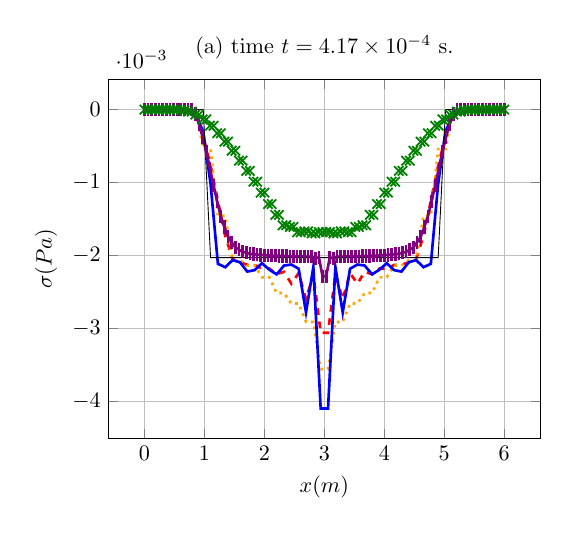
\begin{tikzpicture}[scale=0.8]
\begin{axis}[xlabel=$x (m)$,ylabel=$\sigma (Pa)$,ymajorgrids=true,xmajorgrids=true,legend pos=outer north east,title={(a) time $t = 4.17\times 10^{-4} $ s.}]
\addplot[Red,very thick,mark=none,dashed,mark size=3pt] coordinates {(0.0,0.0) (0.12244897959183673,0.0) (0.24489795918367346,0.0) (0.36734693877551017,0.0) (0.4897959183673469,0.0) (0.6122448979591837,0.0) (0.7346938775510203,0.0) (0.8571428571428571,-6.202478730418737e-05) (0.9795918367346939,-0.00036813096704147385) (1.1020408163265305,-0.0007691528823152809) (1.2244897959183674,-0.0012543541021143585) (1.346938775510204,-0.0017356166211235171) (1.4693877551020407,-0.002048755635913076) (1.5918367346938775,-0.002094430310096999) (1.7142857142857142,-0.0021297551418847207) (1.836734693877551,-0.0021313029263994436) (1.9591836734693877,-0.002184521512510678) (2.0816326530612246,-0.00218056135788198) (2.204081632653061,-0.002258201109747678) (2.326530612244898,-0.002225982674765895) (2.4489795918367347,-0.002388543727551356) (2.571428571428571,-0.002244426952247742) (2.693877551020408,-0.0026005478911843055) (2.816326530612245,-0.0022597626423764634) (2.9387755102040813,-0.003061428019909765) (3.061224489795918,-0.0030614280215042616) (3.183673469387755,-0.0022597625090894887) (3.306122448979592,-0.002600547891240036) (3.4285714285714284,-0.002244427149181305) (3.5510204081632653,-0.002388545096837233) (3.673469387755102,-0.0022259826134320305) (3.7959183673469385,-0.0022582009867140973) (3.9183673469387754,-0.002180561275761312) (4.040816326530612,-0.0021845214357378586) (4.163265306122449,-0.002131302759394598) (4.285714285714286,-0.002129755100625247) (4.408163265306122,-0.002094430313913873) (4.530612244897959,-0.0020487556136377133) (4.653061224489796,-0.0017356165629137574) (4.775510204081632,-0.0012543540420868722) (4.8979591836734695,-0.0007691528306923785) (5.020408163265306,-0.0003681309505408407) (5.142857142857142,-6.202478167641273e-05) (5.26530612244898,0.0) (5.387755102040816,0.0) (5.5102040816326525,0.0) (5.63265306122449,0.0) (5.755102040816326,0.0) (5.877551020408163,0.0) (6.0,0.0) };
\addplot[Orange,very thick,mark=none,dotted,mark size=3pt] coordinates {(0.0,0.0) (0.12244897959183673,0.0) (0.24489795918367346,0.0) (0.36734693877551017,0.0) (0.4897959183673469,0.0) (0.6122448979591837,0.0) (0.7346938775510203,0.0) (0.8571428571428571,0.0) (0.9795918367346939,-0.0005428735747303799) (1.1020408163265305,-0.0005428735744531341) (1.2244897959183674,-0.0014572018602302672) (1.346938775510204,-0.0014572015902572387) (1.4693877551020407,-0.0020650115628520543) (1.5918367346938775,-0.0020650115564237073) (1.7142857142857142,-0.002139129481636798) (1.836734693877551,-0.0021391292444730356) (1.9591836734693877,-0.0022996164460252094) (2.0816326530612246,-0.002299616288054982) (2.204081632653061,-0.002516346947664154) (2.326530612244898,-0.0025163468605162867) (2.4489795918367347,-0.002661476250005421) (2.571428571428571,-0.002661476165813169) (2.693877551020408,-0.002914184951969489) (2.816326530612245,-0.002914184944960401) (2.9387755102040813,-0.0035584423947308316) (3.061224489795918,-0.0035584423949992497) (3.183673469387755,-0.002914184951967428) (3.306122448979592,-0.0029141849534476782) (3.4285714285714284,-0.002661476845762277) (3.5510204081632653,-0.002661476777823057) (3.673469387755102,-0.0025163471827648032) (3.7959183673469385,-0.002516347115664522) (3.9183673469387754,-0.002299616671773065) (4.040816326530612,-0.0022996166084223715) (4.163265306122449,-0.002139129392056909) (4.285714285714286,-0.002139129375421892) (4.408163265306122,-0.002065011745290744) (4.530612244897959,-0.002065011751795016) (4.653061224489796,-0.001457201751052586) (4.775510204081632,-0.0014572017763862047) (4.8979591836734695,-0.000542873542473533) (5.020408163265306,-0.0005428735429029903) (5.142857142857142,0.0) (5.26530612244898,0.0) (5.387755102040816,0.0) (5.5102040816326525,0.0) (5.63265306122449,0.0) (5.755102040816326,0.0) (5.877551020408163,0.0) (6.0,0.0) };
\addplot[Blue,very thick,mark=none,solid,mark size=3pt] coordinates {(0.0,0.0) (0.12244897959183673,0.0) (0.24489795918367346,0.0) (0.36734693877551017,0.0) (0.4897959183673469,0.0) (0.6122448979591837,-6.278098647312321e-06) (0.7346938775510203,-2.4041734526500193e-05) (0.8571428571428571,-8.231252354464475e-05) (0.9795918367346939,-0.0002991596449725322) (1.1020408163265305,-0.0010179588589277829) (1.2244897959183674,-0.00211651125785778) (1.346938775510204,-0.002162627546957125) (1.4693877551020407,-0.002065078047300572) (1.5918367346938775,-0.0020946463817869327) (1.7142857142857142,-0.0022225969088509835) (1.836734693877551,-0.002202804765156386) (1.9591836734693877,-0.002108476200955529) (2.0816326530612246,-0.0021961061957235994) (2.204081632653061,-0.002260872273804215) (2.326530612244898,-0.0021401979709746418) (2.4489795918367347,-0.0021260586132198643) (2.571428571428571,-0.0021835117504344485) (2.693877551020408,-0.0027831455563594575) (2.816326530612245,-0.0021603089312707217) (2.9387755102040813,-0.00410115942266404) (3.061224489795918,-0.00410115942266404) (3.183673469387755,-0.0021603089312707195) (3.306122448979592,-0.0027831455563594575) (3.4285714285714284,-0.0021835117504344498) (3.5510204081632653,-0.0021260586132198643) (3.673469387755102,-0.0021401979709746426) (3.7959183673469385,-0.002260872273804217) (3.9183673469387754,-0.0021961061957235903) (4.040816326530612,-0.002108476200955527) (4.163265306122449,-0.002202804765156385) (4.285714285714286,-0.002222596908850955) (4.408163265306122,-0.00209464638178693) (4.530612244897959,-0.002065078047300569) (4.653061224489796,-0.0021626275469571166) (4.775510204081632,-0.0021165112578577674) (4.8979591836734695,-0.0010179588589277811) (5.020408163265306,-0.0002991596449725306) (5.142857142857142,-8.231252354464585e-05) (5.26530612244898,-2.404173452650139e-05) (5.387755102040816,-6.278098647312686e-06) (5.5102040816326525,0.0) (5.63265306122449,0.0) (5.755102040816326,0.0) (5.877551020408163,0.0) (6.0,0.0) };
\addplot[Purple,very thick,mark=|,solid,mark size=3pt] coordinates {(0.0,0.0) (0.06060606060606061,0.0) (0.12121212121212122,0.0) (0.18181818181818182,0.0) (0.24242424242424243,0.0) (0.30303030303030304,0.0) (0.36363636363636365,0.0) (0.42424242424242425,0.0) (0.48484848484848486,0.0) (0.5454545454545454,0.0) (0.6060606060606061,0.0) (0.6666666666666667,0.0) (0.7272727272727273,0.0) (0.7878787878787878,-2.102087026510683e-10) (0.8484848484848485,-5.933454445134857e-05) (0.9090909090909092,-0.00019666441211383344) (0.9696969696969697,-0.000374409291697533) (1.0303030303030303,-0.0005722648866595782) (1.0909090909090908,-0.0008056893472495531) (1.1515151515151516,-0.001039344553408203) (1.2121212121212122,-0.0012582426511154375) (1.2727272727272727,-0.001463343679322638) (1.3333333333333335,-0.0016127307863671309) (1.393939393939394,-0.0017460505019539665) (1.4545454545454546,-0.0018218179515133914) (1.5151515151515151,-0.0018898271010591291) (1.5757575757575757,-0.0019212706379672865) (1.6363636363636365,-0.0019517753164705633) (1.696969696969697,-0.0019640200241847683) (1.7575757575757576,-0.0019777892349964947) (1.8181818181818183,-0.00198321411930953) (1.878787878787879,-0.0019904956763223034) (1.9393939393939394,-0.001993427920769702) (2.0,-0.0019980258450979097) (2.0606060606060606,-0.0019998696750316023) (2.121212121212121,-0.002003218730140839) (2.1818181818181817,-0.002004470567368423) (2.2424242424242427,-0.0020071540285014795) (2.303030303030303,-0.002007999665063322) (2.3636363636363638,-0.00201032098232525) (2.4242424242424243,-0.0020108541583820755) (2.484848484848485,-0.0020131468962690698) (2.5454545454545454,-0.0020134626237766347) (2.606060606060606,-0.0020161438749334505) (2.666666666666667,-0.002016134393902099) (2.7272727272727275,-0.00201958433697188) (2.787878787878788,-0.0020188214892157487) (2.8484848484848486,-0.0020416792740526437) (2.909090909090909,-0.002026433031381828) (2.9696969696969697,-0.0022869057829180586) (3.0303030303030303,-0.0022869057829180586) (3.090909090909091,-0.00202643303138183) (3.1515151515151514,-0.0020416792740526424) (3.2121212121212124,-0.0020188214892157483) (3.272727272727273,-0.002019584336971879) (3.3333333333333335,-0.0020161343939021) (3.393939393939394,-0.002016143874933451) (3.4545454545454546,-0.002013462623776635) (3.515151515151515,-0.0020131468962690698) (3.5757575757575757,-0.0020108541583820755) (3.6363636363636367,-0.00201032098232525) (3.6969696969696972,-0.0020079996650633225) (3.757575757575758,-0.00200715402850148) (3.8181818181818183,-0.0020044705673684248) (3.878787878787879,-0.002003218730140839) (3.9393939393939394,-0.001999869675031603) (4.0,-0.0019980258450979105) (4.0606060606060606,-0.001993427920769704) (4.121212121212121,-0.0019904956763223043) (4.181818181818182,-0.0019832141193095324) (4.242424242424242,-0.001977789234996496) (4.303030303030303,-0.0019640200241847713) (4.363636363636363,-0.0019517753164705652) (4.424242424242425,-0.001921270637967289) (4.484848484848485,-0.0018898271010591296) (4.545454545454546,-0.001821817951513394) (4.606060606060606,-0.0017460505019539676) (4.666666666666667,-0.0016127307863671332) (4.7272727272727275,-0.001463343679322639) (4.787878787878788,-0.001258242651115441) (4.848484848484849,-0.0010393445534082066) (4.909090909090909,-0.0008056893472495551) (4.96969696969697,-0.0005722648866595818) (5.03030303030303,-0.00037440929169753735) (5.090909090909091,-0.0001966644121138361) (5.151515151515151,-5.933454445134941e-05) (5.212121212121212,-2.1020870265128841e-10) (5.2727272727272725,0.0) (5.333333333333334,0.0) (5.3939393939393945,0.0) (5.454545454545455,0.0) (5.515151515151516,0.0) (5.575757575757576,0.0) (5.636363636363637,0.0) (5.696969696969697,0.0) (5.757575757575758,0.0) (5.818181818181818,0.0) (5.878787878787879,0.0) (5.9393939393939394,0.0) (6.0,0.0) };
\addplot[Green,thick,mark=x,only marks,mark size=3pt] coordinates {(0.0,0.0) (0.06060606060606061,0.0) (0.12121212121212122,0.0) (0.18181818181818182,0.0) (0.24242424242424243,0.0) (0.30303030303030304,0.0) (0.36363636363636365,0.0) (0.42424242424242425,0.0) (0.48484848484848486,0.0) (0.5454545454545454,0.0) (0.6060606060606061,-7.541928868240051e-06) (0.6666666666666667,-7.541928868229345e-06) (0.7272727272727273,-2.7084017957293276e-05) (0.7878787878787878,-2.7084017957300184e-05) (0.8484848484848485,-6.859713739037666e-05) (0.9090909090909092,-6.859713739037584e-05) (0.9696969696969697,-0.0001344887591217594) (1.0303030303030303,-0.00013448875912177324) (1.0909090909090908,-0.00022152236877268994) (1.1515151515151516,-0.00022152236877268793) (1.2121212121212122,-0.0003242523797458477) (1.2727272727272727,-0.0003242523797458495) (1.3333333333333335,-0.0004401175241166998) (1.393939393939394,-0.0004401175241166955) (1.4545454545454546,-0.0005652783736503705) (1.5151515151515151,-0.0005652783736503665) (1.5757575757575757,-0.0007004668759840085) (1.6363636363636365,-0.0007004668759840094) (1.696969696969697,-0.0008407298830150507) (1.7575757575757576,-0.0008407298830150555) (1.8181818181818183,-0.0009896799388507634) (1.878787878787879,-0.0009896799388507537) (1.9393939393939394,-0.0011394881053837696) (2.0,-0.0011394881053837483) (2.0606060606060606,-0.0012962218995730156) (2.121212121212121,-0.001296221899573015) (2.1818181818181817,-0.0014442461283461112) (2.2424242424242427,-0.0014442461283460791) (2.303030303030303,-0.0015870213580057504) (2.3636363636363638,-0.0015870213580057664) (2.4242424242424243,-0.001609952015030185) (2.484848484848485,-0.0016099520150300688) (2.5454545454545454,-0.0016826381193043032) (2.606060606060606,-0.0016826381193043207) (2.666666666666667,-0.0016712124587595317) (2.7272727272727275,-0.0016712124587595961) (2.787878787878788,-0.0016984318779487367) (2.8484848484848486,-0.0016984318779487292) (2.909090909090909,-0.0016803916060842941) (2.9696969696969697,-0.0016803916060843564) (3.0303030303030303,-0.0016803916060841846) (3.090909090909091,-0.0016803916060842375) (3.1515151515151514,-0.0016984318779488911) (3.2121212121212124,-0.001698431877948936) (3.272727272727273,-0.0016712124587594489) (3.3333333333333335,-0.0016712124587594413) (3.393939393939394,-0.0016826381193042644) (3.4545454545454546,-0.0016826381193042119) (3.515151515151515,-0.001609952015029999) (3.5757575757575757,-0.0016099520150300668) (3.6363636363636367,-0.0015870213580056888) (3.6969696969696972,-0.0015870213580057126) (3.757575757575758,-0.0014442461283460722) (3.8181818181818183,-0.001444246128346086) (3.878787878787879,-0.0012962218995730295) (3.9393939393939394,-0.0012962218995730172) (4.0,-0.0011394881053837505) (4.0606060606060606,-0.0011394881053837492) (4.121212121212121,-0.000989679938850742) (4.181818181818182,-0.0009896799388507615) (4.242424242424242,-0.0008407298830150445) (4.303030303030303,-0.0008407298830150564) (4.363636363636363,-0.0007004668759840193) (4.424242424242425,-0.0007004668759840206) (4.484848484848485,-0.0005652783736503635) (4.545454545454546,-0.0005652783736503715) (4.606060606060606,-0.0004401175241167171) (4.666666666666667,-0.0004401175241167155) (4.7272727272727275,-0.00032425237974587187) (4.787878787878788,-0.0003242523797458809) (4.848484848484849,-0.00022152236877269233) (4.909090909090909,-0.00022152236877269926) (4.96969696969697,-0.00013448875912178598) (5.03030303030303,-0.0001344887591217872) (5.090909090909091,-6.859713739045158e-05) (5.151515151515151,-6.859713739045805e-05) (5.212121212121212,-2.7084017957307516e-05) (5.2727272727272725,-2.708401795731454e-05) (5.333333333333334,-7.541928868230607e-06) (5.3939393939393945,-7.541928868233546e-06) (5.454545454545455,0.0) (5.515151515151516,0.0) (5.575757575757576,0.0) (5.636363636363637,0.0) (5.696969696969697,0.0) (5.757575757575758,0.0) (5.818181818181818,0.0) (5.878787878787879,0.0) (5.9393939393939394,0.0) (6.0,0.0) };
\addplot[black,thin,mark=none,solid,mark size=3pt] coordinates {(0.0,-0.0) (0.12244897959183673,-0.0) (0.24489795918367346,-0.0) (0.36734693877551017,-0.0) (0.4897959183673469,-0.0) (0.6122448979591837,-0.0) (0.7346938775510203,-0.0) (0.8571428571428571,-0.0) (0.9795918367346939,-0.0) (1.1020408163265305,-0.002030785796418313) (1.2244897959183674,-0.002030785796418313) (1.346938775510204,-0.002030785796418313) (1.4693877551020407,-0.002030785796418313) (1.5918367346938775,-0.002030785796418313) (1.7142857142857142,-0.002030785796418313) (1.836734693877551,-0.002030785796418313) (1.9591836734693877,-0.002030785796418313) (2.0816326530612246,-0.002030785796418313) (2.204081632653061,-0.002030785796418313) (2.326530612244898,-0.002030785796418313) (2.4489795918367347,-0.002030785796418313) (2.571428571428571,-0.002030785796418313) (2.693877551020408,-0.002030785796418313) (2.816326530612245,-0.002030785796418313) (2.9387755102040813,-0.002030785796418313) (3.061224489795918,-0.002030785796418313) (3.183673469387755,-0.002030785796418313) (3.306122448979592,-0.002030785796418313) (3.4285714285714284,-0.002030785796418313) (3.5510204081632653,-0.002030785796418313) (3.673469387755102,-0.002030785796418313) (3.7959183673469385,-0.002030785796418313) (3.9183673469387754,-0.002030785796418313) (4.040816326530612,-0.002030785796418313) (4.163265306122449,-0.002030785796418313) (4.285714285714286,-0.002030785796418313) (4.408163265306122,-0.002030785796418313) (4.530612244897959,-0.002030785796418313) (4.653061224489796,-0.002030785796418313) (4.775510204081632,-0.002030785796418313) (4.8979591836734695,-0.002030785796418313) (5.020408163265306,-0.0) (5.142857142857142,-0.0) (5.26530612244898,-0.0) (5.387755102040816,-0.0) (5.5102040816326525,-0.0) (5.63265306122449,-0.0) (5.755102040816326,-0.0) (5.877551020408163,-0.0) (6.0,-0.0) };
%\legend{usl 1ppc,usf 1ppc,dgmpm 1ppc,dgmpm 2ppc,dgmpm 2ppc (RK2 + strang),plastic solution}
\end{axis}
\end{tikzpicture}
%%% Local Variables:
%%% mode: latex
%%% TeX-master: "../../mainManuscript"
%%% End:
}
%   {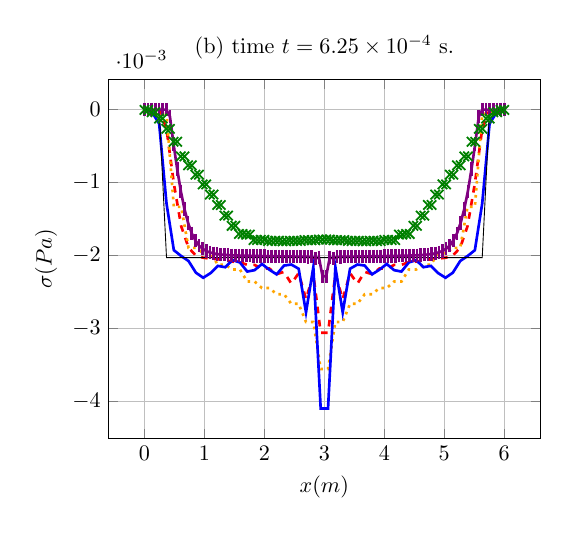
\begin{tikzpicture}[scale=0.8]
\begin{axis}[xlabel=$x (m)$,ylabel=$\sigma (Pa)$,ymajorgrids=true,xmajorgrids=true,legend pos=outer north east,title={(b) time $t = 6.25\times 10^{-4} $ s.}]
\addplot[Red,very thick,mark=none,dashed,mark size=3pt] coordinates {(0.0,0.0) (0.12244897959183673,0.0) (0.24489795918367346,0.0) (0.36734693877551017,-0.00026483849578394367) (0.4897959183673469,-0.001013521443045474) (0.6122448979591837,-0.001599418396582166) (0.7346938775510203,-0.001894897583975942) (0.8571428571428571,-0.002003175763253103) (0.9795918367346939,-0.0020325617224383253) (1.1020408163265305,-0.002045228028080732) (1.2244897959183674,-0.002053732290291538) (1.346938775510204,-0.002068698427659408) (1.4693877551020407,-0.002085802417563694) (1.5918367346938775,-0.002094430310096999) (1.7142857142857142,-0.0021297551418847207) (1.836734693877551,-0.0021313029263994436) (1.9591836734693877,-0.002184521512510678) (2.0816326530612246,-0.00218056135788198) (2.204081632653061,-0.002258201109747678) (2.326530612244898,-0.002225982674765895) (2.4489795918367347,-0.002388543727551356) (2.571428571428571,-0.002244426952247742) (2.693877551020408,-0.0026005478911843055) (2.816326530612245,-0.0022597626423764634) (2.9387755102040813,-0.003061428019909765) (3.061224489795918,-0.0030614280215042616) (3.183673469387755,-0.0022597625090894887) (3.306122448979592,-0.002600547891240036) (3.4285714285714284,-0.002244427149181305) (3.5510204081632653,-0.002388545096837233) (3.673469387755102,-0.0022259826134320305) (3.7959183673469385,-0.0022582009867140973) (3.9183673469387754,-0.002180561275761312) (4.040816326530612,-0.0021845214357378586) (4.163265306122449,-0.002131302759394598) (4.285714285714286,-0.002129755100625247) (4.408163265306122,-0.002094430313913873) (4.530612244897959,-0.002085802281263282) (4.653061224489796,-0.0020686990340733047) (4.775510204081632,-0.002053732101494861) (4.8979591836734695,-0.002045227646988374) (5.020408163265306,-0.002032561293211891) (5.142857142857142,-0.002003175773545243) (5.26530612244898,-0.001894903223389431) (5.387755102040816,-0.0015994182857342976) (5.5102040816326525,-0.0010135213099064534) (5.63265306122449,-0.0002648400904681731) (5.755102040816326,0.0) (5.877551020408163,0.0) (6.0,0.0) };
\addplot[Orange,very thick,mark=none,dotted,mark size=3pt] coordinates {(0.0,0.0) (0.12244897959183673,0.0) (0.24489795918367346,-5.7301755105765905e-05) (0.36734693877551017,-5.730189455576938e-05) (0.4897959183673469,-0.0013347906501971517) (0.6122448979591837,-0.0013347901679111186) (0.7346938775510203,-0.0018978853621068183) (0.8571428571428571,-0.0018978850318875267) (0.9795918367346939,-0.0019688602343015333) (1.1020408163265305,-0.001968859643255841) (1.2244897959183674,-0.0021294179293388526) (1.346938775510204,-0.0021294183868218043) (1.4693877551020407,-0.002194450786388116) (1.5918367346938775,-0.002194450017072264) (1.7142857142857142,-0.002359628639203141) (1.836734693877551,-0.002359632498979967) (1.9591836734693877,-0.0024482611380392057) (2.0816326530612246,-0.0024482617498292327) (2.204081632653061,-0.0025330451235017004) (2.326530612244898,-0.0025330454201282796) (2.4489795918367347,-0.0026644433282951813) (2.571428571428571,-0.002664443159431375) (2.693877551020408,-0.002914184951969489) (2.816326530612245,-0.002914184944960401) (2.9387755102040813,-0.0035584423947308316) (3.061224489795918,-0.0035584423949992497) (3.183673469387755,-0.002914184951967428) (3.306122448979592,-0.0029141849534476782) (3.4285714285714284,-0.002664444198988343) (3.5510204081632653,-0.002664443841077106) (3.673469387755102,-0.0025330448069917346) (3.7959183673469385,-0.002533045701171117) (3.9183673469387754,-0.002448256452448852) (4.040816326530612,-0.002448261928651275) (4.163265306122449,-0.0023596324432405987) (4.285714285714286,-0.0023596329747803267) (4.408163265306122,-0.002194450734585246) (4.530612244897959,-0.002194449738710537) (4.653061224489796,-0.0021294183668896256) (4.775510204081632,-0.002129418349055579) (4.8979591836734695,-0.001968860118219393) (5.020408163265306,-0.0019688594313722226) (5.142857142857142,-0.0018978854498614389) (5.26530612244898,-0.0018978851381802133) (5.387755102040816,-0.0013347904245097116) (5.5102040816326525,-0.001334790188952414) (5.63265306122449,-5.730185243339023e-05) (5.755102040816326,-5.730185485343143e-05) (5.877551020408163,0.0) (6.0,0.0) };
\addplot[Blue,very thick,mark=none,solid,mark size=3pt] coordinates {(0.0,-3.893079067418818e-06) (0.12244897959183673,-3.047957003773611e-05) (0.24489795918367346,-0.000194336720102431) (0.36734693877551017,-0.0012876041625046832) (0.4897959183673469,-0.0019289954950223976) (0.6122448979591837,-0.002009227173232224) (0.7346938775510203,-0.0020777863701164022) (0.8571428571428571,-0.0022375987292720654) (0.9795918367346939,-0.0023072199656024722) (1.1020408163265305,-0.002243560529202433) (1.2244897959183674,-0.0021445098783626536) (1.346938775510204,-0.002162627546957125) (1.4693877551020407,-0.002065314702320964) (1.5918367346938775,-0.0020976556349240846) (1.7142857142857142,-0.0022225969088509835) (1.836734693877551,-0.0022028059756579103) (1.9591836734693877,-0.002118543769523527) (2.0816326530612246,-0.0021961061957235994) (2.204081632653061,-0.002260872273804215) (2.326530612244898,-0.0021401979709746418) (2.4489795918367347,-0.0021260586132198643) (2.571428571428571,-0.0021835117504344485) (2.693877551020408,-0.0027831455563594575) (2.816326530612245,-0.0021603089312707217) (2.9387755102040813,-0.00410115942266404) (3.061224489795918,-0.00410115942266404) (3.183673469387755,-0.0021603089312707195) (3.306122448979592,-0.0027831455563594575) (3.4285714285714284,-0.0021835117504344498) (3.5510204081632653,-0.0021260586132198643) (3.673469387755102,-0.0021401979709746426) (3.7959183673469385,-0.002260872273804217) (3.9183673469387754,-0.0021961061957235903) (4.040816326530612,-0.002118543769523527) (4.163265306122449,-0.002202805975657909) (4.285714285714286,-0.002222596908850955) (4.408163265306122,-0.0020976556349240833) (4.530612244897959,-0.0020653147023209618) (4.653061224489796,-0.0021626275469571166) (4.775510204081632,-0.0021445098783626554) (4.8979591836734695,-0.002243560529202434) (5.020408163265306,-0.002307219965602473) (5.142857142857142,-0.0022375987292720598) (5.26530612244898,-0.002077786370116406) (5.387755102040816,-0.002009227173232226) (5.5102040816326525,-0.0019289954950223924) (5.63265306122449,-0.0012876041625046687) (5.755102040816326,-0.00019433672010243214) (5.877551020408163,-3.047957003773766e-05) (6.0,-3.89307906741869e-06) };
\addplot[Purple,very thick,mark=|,solid,mark size=3pt] coordinates {(0.0,0.0) (0.06060606060606061,0.0) (0.12121212121212122,0.0) (0.18181818181818182,0.0) (0.24242424242424243,0.0) (0.30303030303030304,0.0) (0.36363636363636365,0.0) (0.42424242424242425,-9.478454557786464e-05) (0.48484848484848486,-0.0004733763203636077) (0.5454545454545454,-0.000814341803859037) (0.6060606060606061,-0.00111922644858282) (0.6666666666666667,-0.0013639777840079603) (0.7272727272727273,-0.0015544317104102714) (0.7878787878787878,-0.0016969397043999374) (0.8484848484848485,-0.0017949331499141452) (0.9090909090909092,-0.0018654199222256865) (0.9696969696969697,-0.0019091603206922254) (1.0303030303030303,-0.0019406187410981471) (1.0909090909090908,-0.0019590334022499775) (1.1515151515151516,-0.001973016484643746) (1.2121212121212122,-0.0019812974809459826) (1.2727272727272727,-0.0019882165408146835) (1.3333333333333335,-0.001992517920818215) (1.393939393939394,-0.00199644892142901) (1.4545454545454546,-0.001998847531766857) (1.5151515151515151,-0.0020012976353965943) (1.5757575757575757,-0.002002723340276947) (1.6363636363636365,-0.0020044767003141563) (1.696969696969697,-0.002005455954611059) (1.7575757575757576,-0.0020068717566027695) (1.8181818181818183,-0.0020076243914485758) (1.878787878787879,-0.0020088510479386633) (1.9393939393939394,-0.0020094619562297344) (2.0,-0.0020105817510746183) (2.0606060606060606,-0.002011097015992123) (2.121212121212121,-0.0020121761338987108) (2.1818181818181817,-0.0020126171467676774) (2.2424242424242427,-0.0020136968548150214) (2.303030303030303,-0.0020140562994433687) (2.3636363636363638,-0.002015172057998995) (2.4242424242424243,-0.0020154349921928374) (2.484848484848485,-0.0020167112186900084) (2.5454545454545454,-0.002016887611422729) (2.606060606060606,-0.0020185925173496996) (2.666666666666667,-0.002018578059346721) (2.7272727272727275,-0.002021063173066831) (2.787878787878788,-0.0020204807134743753) (2.8484848484848486,-0.0020416794860022825) (2.909090909090909,-0.002026827362087739) (2.9696969696969697,-0.0022869057829180586) (3.0303030303030303,-0.0022869057829180586) (3.090909090909091,-0.002026827362087741) (3.1515151515151514,-0.002041679486002281) (3.2121212121212124,-0.0020204807134743753) (3.272727272727273,-0.0020210631730668296) (3.3333333333333335,-0.0020185780593467225) (3.393939393939394,-0.0020185925173497004) (3.4545454545454546,-0.0020168876114227295) (3.515151515151515,-0.002016711218690009) (3.5757575757575757,-0.002015434992192838) (3.6363636363636367,-0.0020151720579989953) (3.6969696969696972,-0.002014056299443369) (3.757575757575758,-0.0020136968548150227) (3.8181818181818183,-0.002012617146767679) (3.878787878787879,-0.0020121761338987108) (3.9393939393939394,-0.002011097015992124) (4.0,-0.002010581751074619) (4.0606060606060606,-0.0020094619562297353) (4.121212121212121,-0.0020088510479386638) (4.181818181818182,-0.002007624391448577) (4.242424242424242,-0.00200687175660277) (4.303030303030303,-0.002005455954611061) (4.363636363636363,-0.0020044767003141568) (4.424242424242425,-0.0020027233402769486) (4.484848484848485,-0.002001297635396595) (4.545454545454546,-0.0019988475317668586) (4.606060606060606,-0.0019964489214290117) (4.666666666666667,-0.0019925179208182173) (4.7272727272727275,-0.0019882165408146857) (4.787878787878788,-0.0019812974809459843) (4.848484848484849,-0.0019730164846437476) (4.909090909090909,-0.0019590334022499805) (4.96969696969697,-0.0019406187410981489) (5.03030303030303,-0.0019091603206922276) (5.090909090909091,-0.001865419922225688) (5.151515151515151,-0.0017949331499141465) (5.212121212121212,-0.0016969397043999379) (5.2727272727272725,-0.0015544317104102714) (5.333333333333334,-0.0013639777840079614) (5.3939393939393945,-0.0011192264485828216) (5.454545454545455,-0.0008143418038590386) (5.515151515151516,-0.0004733763203636097) (5.575757575757576,-9.478454557786505e-05) (5.636363636363637,0.0) (5.696969696969697,0.0) (5.757575757575758,0.0) (5.818181818181818,0.0) (5.878787878787879,0.0) (5.9393939393939394,0.0) (6.0,0.0) };
\addplot[Green,thick,mark=x,only marks,mark size=3pt] coordinates {(0.0,-4.653556676445113e-06) (0.06060606060606061,-4.653556676466522e-06) (0.12121212121212122,-3.553597365446572e-05) (0.18181818181818182,-3.553597365448185e-05) (0.24242424242424243,-0.00012281470180235295) (0.30303030303030304,-0.00012281470180237252) (0.36363636363636365,-0.00026409308529461167) (0.42424242424242425,-0.0002640930852946001) (0.48484848484848486,-0.00044103089416509117) (0.5454545454545454,-0.0004410308941650814) (0.6060606060606061,-0.000641965342651722) (0.6666666666666667,-0.0006419653426517044) (0.7272727272727273,-0.0007642218788261203) (0.7878787878787878,-0.000764221878826115) (0.8484848484848485,-0.0008928462121140367) (0.9090909090909092,-0.0008928462121140418) (0.9696969696969697,-0.0010267020703216654) (1.0303030303030303,-0.0010267020703216743) (1.0909090909090908,-0.0011658963775695353) (1.1515151515151516,-0.0011658963775695475) (1.2121212121212122,-0.0013084847600696925) (1.2727272727272727,-0.0013084847600697092) (1.3333333333333335,-0.0014547578806386335) (1.393939393939394,-0.001454757880638625) (1.4545454545454546,-0.0015944875452197276) (1.5151515151515151,-0.0015944875452197434) (1.5757575757575757,-0.001707074178639678) (1.6363636363636365,-0.0017070741786396851) (1.696969696969697,-0.0017150623709443888) (1.7575757575757576,-0.001715062370944398) (1.8181818181818183,-0.001790298875206909) (1.878787878787879,-0.0017902988752067975) (1.9393939393939394,-0.0017871999380725328) (2.0,-0.0017871999380725146) (2.0606060606060606,-0.0018039003213189228) (2.121212121212121,-0.0018039003213188086) (2.1818181818181817,-0.0018002331089720413) (2.2424242424242427,-0.0018002331089720298) (2.303030303030303,-0.0018066356526349138) (2.3636363636363638,-0.001806635652634928) (2.4242424242424243,-0.0018005119579068544) (2.484848484848485,-0.001800511957906827) (2.5454545454545454,-0.0018027419309853173) (2.606060606060606,-0.001802741930985315) (2.666666666666667,-0.0017908982789932382) (2.7272727272727275,-0.0017908982789932527) (2.787878787878788,-0.0017920432553689817) (2.8484848484848486,-0.0017920432553690704) (2.909090909090909,-0.0017832541467531172) (2.9696969696969697,-0.001783254146753207) (3.0303030303030303,-0.0017832541467531968) (3.090909090909091,-0.0017832541467532597) (3.1515151515151514,-0.001792043255369177) (3.2121212121212124,-0.001792043255369262) (3.272727272727273,-0.0017908982789931235) (3.3333333333333335,-0.0017908982789931267) (3.393939393939394,-0.0018027419309851842) (3.4545454545454546,-0.00180274193098518) (3.515151515151515,-0.0018005119579067273) (3.5757575757575757,-0.0018005119579067206) (3.6363636363636367,-0.0018066356526347171) (3.6969696969696972,-0.001806635652634705) (3.757575757575758,-0.0018002331089718607) (3.8181818181818183,-0.0018002331089718572) (3.878787878787879,-0.0018039003213187017) (3.9393939393939394,-0.0018039003213188207) (4.0,-0.0017871999380728316) (4.0606060606060606,-0.001787199938072803) (4.121212121212121,-0.0017902988752070415) (4.181818181818182,-0.001790298875207153) (4.242424242424242,-0.0017150623709445087) (4.303030303030303,-0.0017150623709445115) (4.363636363636363,-0.001707074178639759) (4.424242424242425,-0.0017070741786397732) (4.484848484848485,-0.0015944875452197688) (4.545454545454546,-0.0015944875452197464) (4.606060606060606,-0.0014547578806386077) (4.666666666666667,-0.0014547578806386094) (4.7272727272727275,-0.0013084847600697066) (4.787878787878788,-0.0013084847600697033) (4.848484848484849,-0.0011658963775695345) (4.909090909090909,-0.0011658963775695356) (4.96969696969697,-0.001026702070321666) (5.03030303030303,-0.0010267020703216456) (5.090909090909091,-0.0008928462121140489) (5.151515151515151,-0.0008928462121140479) (5.212121212121212,-0.0007642218788261214) (5.2727272727272725,-0.0007642218788261214) (5.333333333333334,-0.0006419653426517155) (5.3939393939393945,-0.0006419653426517138) (5.454545454545455,-0.000441030894165099) (5.515151515151516,-0.0004410308941651111) (5.575757575757576,-0.00026409308529464273) (5.636363636363637,-0.0002640930852946408) (5.696969696969697,-0.0001228147018024683) (5.757575757575758,-0.0001228147018024451) (5.818181818181818,-3.553597365452076e-05) (5.878787878787879,-3.553597365451883e-05) (5.9393939393939394,-4.653556676452633e-06) (6.0,-4.653556676488362e-06) };
\addplot[black,thin,mark=none,solid,mark size=3pt] coordinates {(0.0,-0.0) (0.12244897959183673,-0.0) (0.24489795918367346,-0.0) (0.36734693877551017,-0.002030785796418313) (0.4897959183673469,-0.002030785796418313) (0.6122448979591837,-0.002030785796418313) (0.7346938775510203,-0.002030785796418313) (0.8571428571428571,-0.002030785796418313) (0.9795918367346939,-0.002030785796418313) (1.1020408163265305,-0.002030785796418313) (1.2244897959183674,-0.002030785796418313) (1.346938775510204,-0.002030785796418313) (1.4693877551020407,-0.002030785796418313) (1.5918367346938775,-0.002030785796418313) (1.7142857142857142,-0.002030785796418313) (1.836734693877551,-0.002030785796418313) (1.9591836734693877,-0.002030785796418313) (2.0816326530612246,-0.002030785796418313) (2.204081632653061,-0.002030785796418313) (2.326530612244898,-0.002030785796418313) (2.4489795918367347,-0.002030785796418313) (2.571428571428571,-0.002030785796418313) (2.693877551020408,-0.002030785796418313) (2.816326530612245,-0.002030785796418313) (2.9387755102040813,-0.002030785796418313) (3.061224489795918,-0.002030785796418313) (3.183673469387755,-0.002030785796418313) (3.306122448979592,-0.002030785796418313) (3.4285714285714284,-0.002030785796418313) (3.5510204081632653,-0.002030785796418313) (3.673469387755102,-0.002030785796418313) (3.7959183673469385,-0.002030785796418313) (3.9183673469387754,-0.002030785796418313) (4.040816326530612,-0.002030785796418313) (4.163265306122449,-0.002030785796418313) (4.285714285714286,-0.002030785796418313) (4.408163265306122,-0.002030785796418313) (4.530612244897959,-0.002030785796418313) (4.653061224489796,-0.002030785796418313) (4.775510204081632,-0.002030785796418313) (4.8979591836734695,-0.002030785796418313) (5.020408163265306,-0.002030785796418313) (5.142857142857142,-0.002030785796418313) (5.26530612244898,-0.002030785796418313) (5.387755102040816,-0.002030785796418313) (5.5102040816326525,-0.002030785796418313) (5.63265306122449,-0.002030785796418313) (5.755102040816326,-0.0) (5.877551020408163,-0.0) (6.0,-0.0) };
%\legend{usl 1ppc,usf 1ppc,dgmpm 1ppc,dgmpm 2ppc,dgmpm 2ppc (RK2 + strang),plastic solution}
\end{axis}
\end{tikzpicture}
%%% Local Variables:
%%% mode: latex
%%% TeX-master: "../../mainManuscript"
%%% End:
}
%   {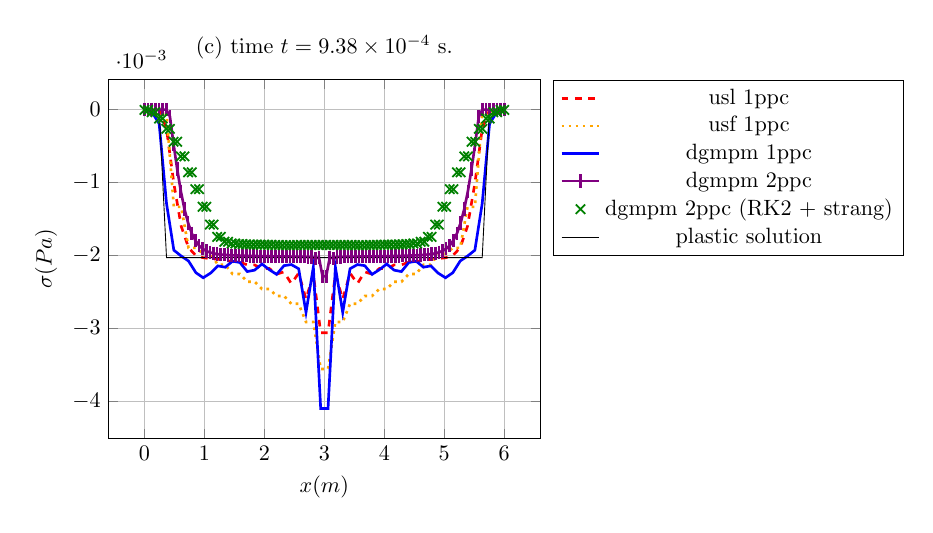
\begin{tikzpicture}[scale=0.8]
\begin{axis}[xlabel=$x (m)$,ylabel=$\sigma (Pa)$,ymajorgrids=true,xmajorgrids=true,legend pos=outer north east,title={(c) time $t = 9.38\times 10^{-4} $ s.}]
\addplot[Red,very thick,mark=none,dashed,mark size=3pt] coordinates {(0.0,0.0) (0.12244897959183673,0.0) (0.24489795918367346,0.0) (0.36734693877551017,-0.00026483849578394367) (0.4897959183673469,-0.001013521443045474) (0.6122448979591837,-0.001599418396582166) (0.7346938775510203,-0.001894897583975942) (0.8571428571428571,-0.002003175763253103) (0.9795918367346939,-0.0020325617224383253) (1.1020408163265305,-0.002045228028080732) (1.2244897959183674,-0.002053732290291538) (1.346938775510204,-0.002068698427659408) (1.4693877551020407,-0.002085802417563694) (1.5918367346938775,-0.002094430310096999) (1.7142857142857142,-0.0021297551418847207) (1.836734693877551,-0.0021313029263994436) (1.9591836734693877,-0.002184521512510678) (2.0816326530612246,-0.00218056135788198) (2.204081632653061,-0.002258201109747678) (2.326530612244898,-0.002225982674765895) (2.4489795918367347,-0.002388543727551356) (2.571428571428571,-0.002244426952247742) (2.693877551020408,-0.0026005478911843055) (2.816326530612245,-0.0022597626423764634) (2.9387755102040813,-0.003061428019909765) (3.061224489795918,-0.0030614280215042616) (3.183673469387755,-0.0022597625090894887) (3.306122448979592,-0.002600547891240036) (3.4285714285714284,-0.002244427149181305) (3.5510204081632653,-0.002388545096837233) (3.673469387755102,-0.0022259826134320305) (3.7959183673469385,-0.0022582009867140973) (3.9183673469387754,-0.002180561275761312) (4.040816326530612,-0.0021845214357378586) (4.163265306122449,-0.002131302759394598) (4.285714285714286,-0.002129755100625247) (4.408163265306122,-0.002094430313913873) (4.530612244897959,-0.002085802281263282) (4.653061224489796,-0.0020686990340733047) (4.775510204081632,-0.002053732101494861) (4.8979591836734695,-0.002045227646988374) (5.020408163265306,-0.002032561293211891) (5.142857142857142,-0.002003175773545243) (5.26530612244898,-0.001894903223389431) (5.387755102040816,-0.0015994182857342976) (5.5102040816326525,-0.0010135213099064534) (5.63265306122449,-0.0002648400904681731) (5.755102040816326,0.0) (5.877551020408163,0.0) (6.0,0.0) };
\addplot[Orange,very thick,mark=none,dotted,mark size=3pt] coordinates {(0.0,0.0) (0.12244897959183673,0.0) (0.24489795918367346,-5.7301755105765905e-05) (0.36734693877551017,-5.730189455576938e-05) (0.4897959183673469,-0.0013347906501971517) (0.6122448979591837,-0.0013347901679111186) (0.7346938775510203,-0.0018978853621068183) (0.8571428571428571,-0.0018978850318875267) (0.9795918367346939,-0.0019799715434199354) (1.1020408163265305,-0.0019799696050827615) (1.2244897959183674,-0.0021294179293388526) (1.346938775510204,-0.0021294183868218043) (1.4693877551020407,-0.002255946410111241) (1.5918367346938775,-0.0022559455216042603) (1.7142857142857142,-0.0023619885239961427) (1.836734693877551,-0.002361991742698304) (1.9591836734693877,-0.0024610525543925722) (2.0816326530612246,-0.0024610535623674854) (2.204081632653061,-0.0025567250194484252) (2.326530612244898,-0.002556724888093118) (2.4489795918367347,-0.002664443582915471) (2.571428571428571,-0.002664443413600718) (2.693877551020408,-0.002914184951969489) (2.816326530612245,-0.002914184944960401) (2.9387755102040813,-0.0035584423947308316) (3.061224489795918,-0.0035584423949992497) (3.183673469387755,-0.002914184951967428) (3.306122448979592,-0.0029141849534476782) (3.4285714285714284,-0.0026644444535014193) (3.5510204081632653,-0.0026644440952976736) (3.673469387755102,-0.0025567222026880295) (3.7959183673469385,-0.002556725323601323) (3.9183673469387754,-0.0024610504976733446) (4.040816326530612,-0.0024610474461122947) (4.163265306122449,-0.002361991399376669) (4.285714285714286,-0.0023619921199265104) (4.408163265306122,-0.0022559465145723435) (4.530612244897959,-0.002255946104769913) (4.653061224489796,-0.0021294183668896256) (4.775510204081632,-0.002129418349055579) (4.8979591836734695,-0.001979970026467421) (5.020408163265306,-0.001979969550242234) (5.142857142857142,-0.0018978854498614389) (5.26530612244898,-0.0018978851381802133) (5.387755102040816,-0.0013347904245097116) (5.5102040816326525,-0.001334790188952414) (5.63265306122449,-5.730185243339023e-05) (5.755102040816326,-5.730185485343143e-05) (5.877551020408163,0.0) (6.0,0.0) };
\addplot[Blue,very thick,mark=none,solid,mark size=3pt] coordinates {(0.0,-3.893079067418818e-06) (0.12244897959183673,-3.047957003773611e-05) (0.24489795918367346,-0.000194336720102431) (0.36734693877551017,-0.0012876041625046832) (0.4897959183673469,-0.0019289954950223976) (0.6122448979591837,-0.002009227173232224) (0.7346938775510203,-0.0020777863701164022) (0.8571428571428571,-0.0022375987292720654) (0.9795918367346939,-0.0023072199656024722) (1.1020408163265305,-0.002243560529202433) (1.2244897959183674,-0.0021445098783626536) (1.346938775510204,-0.002162627546957125) (1.4693877551020407,-0.0020802167627439966) (1.5918367346938775,-0.0020981207023951175) (1.7142857142857142,-0.0022225969088509835) (1.836734693877551,-0.0022028059756579103) (1.9591836734693877,-0.002118543769523527) (2.0816326530612246,-0.0021961061957235994) (2.204081632653061,-0.002260872273804215) (2.326530612244898,-0.0021414564292731074) (2.4489795918367347,-0.00212638789674907) (2.571428571428571,-0.0021835117504344485) (2.693877551020408,-0.0027831455563594575) (2.816326530612245,-0.0021603089312707217) (2.9387755102040813,-0.00410115942266404) (3.061224489795918,-0.00410115942266404) (3.183673469387755,-0.0021603089312707195) (3.306122448979592,-0.0027831455563594575) (3.4285714285714284,-0.0021835117504344498) (3.5510204081632653,-0.0021263878967490695) (3.673469387755102,-0.002141456429273106) (3.7959183673469385,-0.002260872273804217) (3.9183673469387754,-0.0021961061957235903) (4.040816326530612,-0.002118543769523527) (4.163265306122449,-0.002202805975657909) (4.285714285714286,-0.002222596908850955) (4.408163265306122,-0.002098120702395116) (4.530612244897959,-0.0020802167627439914) (4.653061224489796,-0.0021626275469571166) (4.775510204081632,-0.0021445098783626554) (4.8979591836734695,-0.002243560529202434) (5.020408163265306,-0.002307219965602473) (5.142857142857142,-0.0022375987292720598) (5.26530612244898,-0.002077786370116406) (5.387755102040816,-0.002009227173232226) (5.5102040816326525,-0.0019289954950223924) (5.63265306122449,-0.0012876041625046687) (5.755102040816326,-0.00019433672010243214) (5.877551020408163,-3.047957003773766e-05) (6.0,-3.89307906741869e-06) };
\addplot[Purple,very thick,mark=|,solid,mark size=3pt] coordinates {(0.0,0.0) (0.06060606060606061,0.0) (0.12121212121212122,0.0) (0.18181818181818182,0.0) (0.24242424242424243,0.0) (0.30303030303030304,0.0) (0.36363636363636365,0.0) (0.42424242424242425,-9.478454557786464e-05) (0.48484848484848486,-0.0004733763203636077) (0.5454545454545454,-0.000814341803859037) (0.6060606060606061,-0.00111922644858282) (0.6666666666666667,-0.0013639777840079603) (0.7272727272727273,-0.0015544317104102714) (0.7878787878787878,-0.0016969397043999374) (0.8484848484848485,-0.0017949331499141452) (0.9090909090909092,-0.0018654199222256865) (0.9696969696969697,-0.0019091603206922254) (1.0303030303030303,-0.0019406187410981471) (1.0909090909090908,-0.0019590334022499775) (1.1515151515151516,-0.001973016484643746) (1.2121212121212122,-0.0019812974809459826) (1.2727272727272727,-0.0019882165408146835) (1.3333333333333335,-0.001992525389453014) (1.393939393939394,-0.0019965113731305923) (1.4545454545454546,-0.001999100939983271) (1.5151515151515151,-0.0020017249612510587) (1.5757575757575757,-0.002003462001064455) (1.6363636363636365,-0.0020053719644469842) (1.696969696969697,-0.002006626024245638) (1.7575757575757576,-0.0020081163691946526) (1.8181818181818183,-0.0020090627111062705) (1.878787878787879,-0.0020102875475510175) (1.9393939393939394,-0.002011023705629533) (2.0,-0.002012086457608482) (2.0606060606060606,-0.002012679824059095) (2.121212121212121,-0.002013661625514785) (2.1818181818181817,-0.002014151671599789) (2.2424242424242427,-0.0020151047519611333) (2.303030303030303,-0.0020154999818260636) (2.3636363636363638,-0.0020164657004306443) (2.4242424242424243,-0.002016762219229968) (2.484848484848485,-0.002017851047541544) (2.5454545454545454,-0.002018060271541896) (2.606060606060606,-0.0020195095289608886) (2.666666666666667,-0.002019544598948779) (2.7272727272727275,-0.0020216931102238138) (2.787878787878788,-0.002021218517351617) (2.8484848484848486,-0.0020416794865166367) (2.909090909090909,-0.0020270053009242613) (2.9696969696969697,-0.0022869057829180586) (3.0303030303030303,-0.0022869057829180586) (3.090909090909091,-0.002027005300924263) (3.1515151515151514,-0.0020416794865166354) (3.2121212121212124,-0.002021218517351617) (3.272727272727273,-0.0020216931102238125) (3.3333333333333335,-0.0020195445989487793) (3.393939393939394,-0.0020195095289608895) (3.4545454545454546,-0.002018060271541896) (3.515151515151515,-0.0020178510475415442) (3.5757575757575757,-0.0020167622192299684) (3.6363636363636367,-0.0020164657004306447) (3.6969696969696972,-0.002015499981826064) (3.757575757575758,-0.002015104751961135) (3.8181818181818183,-0.00201415167159979) (3.878787878787879,-0.002013661625514785) (3.9393939393939394,-0.0020126798240590964) (4.0,-0.0020120864576084834) (4.0606060606060606,-0.002011023705629534) (4.121212121212121,-0.0020102875475510183) (4.181818181818182,-0.0020090627111062722) (4.242424242424242,-0.002008116369194653) (4.303030303030303,-0.00200662602424564) (4.363636363636363,-0.0020053719644469847) (4.424242424242425,-0.002003462001064457) (4.484848484848485,-0.00200172496125106) (4.545454545454546,-0.001999100939983273) (4.606060606060606,-0.001996511373130594) (4.666666666666667,-0.001992525389453016) (4.7272727272727275,-0.0019882165408146857) (4.787878787878788,-0.0019812974809459843) (4.848484848484849,-0.0019730164846437476) (4.909090909090909,-0.0019590334022499805) (4.96969696969697,-0.0019406187410981489) (5.03030303030303,-0.0019091603206922276) (5.090909090909091,-0.001865419922225688) (5.151515151515151,-0.0017949331499141465) (5.212121212121212,-0.0016969397043999379) (5.2727272727272725,-0.0015544317104102714) (5.333333333333334,-0.0013639777840079614) (5.3939393939393945,-0.0011192264485828216) (5.454545454545455,-0.0008143418038590386) (5.515151515151516,-0.0004733763203636097) (5.575757575757576,-9.478454557786505e-05) (5.636363636363637,0.0) (5.696969696969697,0.0) (5.757575757575758,0.0) (5.818181818181818,0.0) (5.878787878787879,0.0) (5.9393939393939394,0.0) (6.0,0.0) };
\addplot[Green,thick,mark=x,only marks,mark size=3pt] coordinates {(0.0,-4.653556676445113e-06) (0.06060606060606061,-4.653556676466522e-06) (0.12121212121212122,-3.553597365446572e-05) (0.18181818181818182,-3.553597365448185e-05) (0.24242424242424243,-0.00012281470180235295) (0.30303030303030304,-0.00012281470180237252) (0.36363636363636365,-0.00026409308529461167) (0.42424242424242425,-0.0002640930852946001) (0.48484848484848486,-0.00044103089416509117) (0.5454545454545454,-0.0004410308941650814) (0.6060606060606061,-0.000641965342651722) (0.6666666666666667,-0.0006419653426517044) (0.7272727272727273,-0.0008602957608430413) (0.7878787878787878,-0.000860295760843045) (0.8484848484848485,-0.0010918231411856081) (0.9090909090909092,-0.0010918231411856073) (0.9696969696969697,-0.001333186697345266) (1.0303030303030303,-0.0013331866973452686) (1.0909090909090908,-0.0015780176505098878) (1.1515151515151516,-0.001578017650510065) (1.2121212121212122,-0.0017462722499425219) (1.2727272727272727,-0.0017462722499425203) (1.3333333333333335,-0.0018139377509087903) (1.393939393939394,-0.001813937750908789) (1.4545454545454546,-0.0018370683644219558) (1.5151515151515151,-0.0018370683644219647) (1.5757575757575757,-0.0018446947711792956) (1.6363636363636365,-0.0018446947711792919) (1.696969696969697,-0.0018496271877845487) (1.7575757575757576,-0.0018496271877845641) (1.8181818181818183,-0.0018523990010130002) (1.878787878787879,-0.0018523990010129794) (1.9393939393939394,-0.001853855933079991) (2.0,-0.0018538559330799783) (2.0606060606060606,-0.0018554941823953556) (2.121212121212121,-0.0018554941823953148) (2.1818181818181817,-0.001857719742751121) (2.2424242424242427,-0.0018577197427511259) (2.303030303030303,-0.0018594235513565726) (2.3636363636363638,-0.0018594235513565635) (2.4242424242424243,-0.001860428657234033) (2.484848484848485,-0.0018604286572341492) (2.5454545454545454,-0.0018576938929393341) (2.606060606060606,-0.0018576938929393053) (2.666666666666667,-0.0018583535136019447) (2.7272727272727275,-0.0018583535136019224) (2.787878787878788,-0.0018577492901618203) (2.8484848484848486,-0.001857749290161877) (2.909090909090909,-0.0018577492525243859) (2.9696969696969697,-0.0018577492525244613) (3.0303030303030303,-0.0018577492525243587) (3.090909090909091,-0.0018577492525244195) (3.1515151515151514,-0.0018577492901619775) (3.2121212121212124,-0.0018577492901620057) (3.272727272727273,-0.0018583535136019876) (3.3333333333333335,-0.0018583535136019545) (3.393939393939394,-0.001857693892939594) (3.4545454545454546,-0.0018576938929395622) (3.515151515151515,-0.0018604286572344694) (3.5757575757575757,-0.0018604286572344898) (3.6363636363636367,-0.0018594235513569436) (3.6969696969696972,-0.0018594235513568977) (3.757575757575758,-0.0018577197427509507) (3.8181818181818183,-0.0018577197427510114) (3.878787878787879,-0.001855494182395198) (3.9393939393939394,-0.001855494182395278) (4.0,-0.001853855933079923) (4.0606060606060606,-0.0018538559330798874) (4.121212121212121,-0.0018523990010130078) (4.181818181818182,-0.00185239900101302) (4.242424242424242,-0.0018496271877846608) (4.303030303030303,-0.001849627187784682) (4.363636363636363,-0.0018446947711793316) (4.424242424242425,-0.0018446947711793795) (4.484848484848485,-0.0018370683644221752) (4.545454545454546,-0.0018370683644221035) (4.606060606060606,-0.0018139377509086092) (4.666666666666667,-0.0018139377509087265) (4.7272727272727275,-0.0017462722499428354) (4.787878787878788,-0.001746272249942797) (4.848484848484849,-0.0015780176505098744) (4.909090909090909,-0.0015780176505099757) (4.96969696969697,-0.001333186697345246) (5.03030303030303,-0.0013331866973452415) (5.090909090909091,-0.0010918231411856114) (5.151515151515151,-0.0010918231411856042) (5.212121212121212,-0.000860295760843038) (5.2727272727272725,-0.0008602957608430409) (5.333333333333334,-0.0006419653426517155) (5.3939393939393945,-0.0006419653426517138) (5.454545454545455,-0.000441030894165099) (5.515151515151516,-0.0004410308941651111) (5.575757575757576,-0.00026409308529464273) (5.636363636363637,-0.0002640930852946408) (5.696969696969697,-0.0001228147018024683) (5.757575757575758,-0.0001228147018024451) (5.818181818181818,-3.553597365452076e-05) (5.878787878787879,-3.553597365451883e-05) (5.9393939393939394,-4.653556676452633e-06) (6.0,-4.653556676488362e-06) };
\addplot[black,thin,mark=none,solid,mark size=3pt] coordinates {(0.0,-0.0) (0.12244897959183673,-0.0) (0.24489795918367346,-0.0) (0.36734693877551017,-0.002030785796418313) (0.4897959183673469,-0.002030785796418313) (0.6122448979591837,-0.002030785796418313) (0.7346938775510203,-0.002030785796418313) (0.8571428571428571,-0.002030785796418313) (0.9795918367346939,-0.002030785796418313) (1.1020408163265305,-0.002030785796418313) (1.2244897959183674,-0.002030785796418313) (1.346938775510204,-0.002030785796418313) (1.4693877551020407,-0.002030785796418313) (1.5918367346938775,-0.002030785796418313) (1.7142857142857142,-0.002030785796418313) (1.836734693877551,-0.002030785796418313) (1.9591836734693877,-0.002030785796418313) (2.0816326530612246,-0.002030785796418313) (2.204081632653061,-0.002030785796418313) (2.326530612244898,-0.002030785796418313) (2.4489795918367347,-0.002030785796418313) (2.571428571428571,-0.002030785796418313) (2.693877551020408,-0.002030785796418313) (2.816326530612245,-0.002030785796418313) (2.9387755102040813,-0.002030785796418313) (3.061224489795918,-0.002030785796418313) (3.183673469387755,-0.002030785796418313) (3.306122448979592,-0.002030785796418313) (3.4285714285714284,-0.002030785796418313) (3.5510204081632653,-0.002030785796418313) (3.673469387755102,-0.002030785796418313) (3.7959183673469385,-0.002030785796418313) (3.9183673469387754,-0.002030785796418313) (4.040816326530612,-0.002030785796418313) (4.163265306122449,-0.002030785796418313) (4.285714285714286,-0.002030785796418313) (4.408163265306122,-0.002030785796418313) (4.530612244897959,-0.002030785796418313) (4.653061224489796,-0.002030785796418313) (4.775510204081632,-0.002030785796418313) (4.8979591836734695,-0.002030785796418313) (5.020408163265306,-0.002030785796418313) (5.142857142857142,-0.002030785796418313) (5.26530612244898,-0.002030785796418313) (5.387755102040816,-0.002030785796418313) (5.5102040816326525,-0.002030785796418313) (5.63265306122449,-0.002030785796418313) (5.755102040816326,-0.0) (5.877551020408163,-0.0) (6.0,-0.0) };
\legend{usl 1ppc,usf 1ppc,dgmpm 1ppc,dgmpm 2ppc,dgmpm 2ppc (RK2 + strang),plastic solution}
\end{axis}
\end{tikzpicture}
%%% Local Variables:
%%% mode: latex
%%% TeX-master: "../../mainManuscript"
%%% End:
}
%   \caption{elastic-viscoplastic RP epsp (stiff)}
%   \label{fig:epsp_elastoviscoplastic_RP}
% \end{figure}

\subsubsection{Elastoplasticicity}
Comparison with mpm for 1ppc which does not involve the treatment of rhs and so the choice of some parameter for integrating it.
\begin{figure}[h!]
  \centering
  % {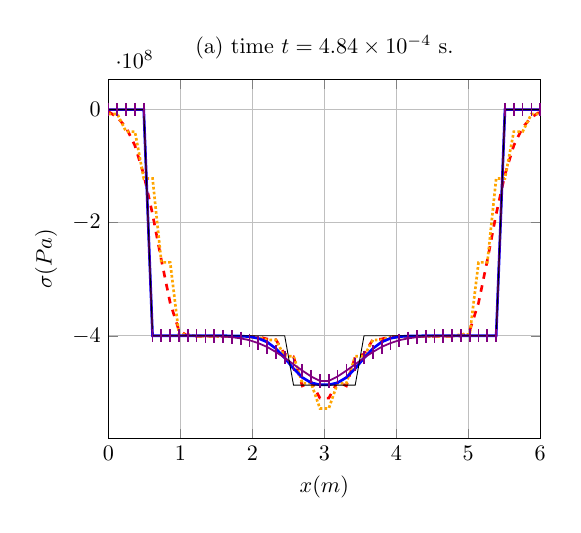
\begin{tikzpicture}[scale=0.8]
\begin{axis}[xlabel=$x (m)$,ylabel=$\sigma (Pa)$,ymajorgrids=true,xmajorgrids=true,legend pos=outer north east,title={(a) time $t = 4.84\times 10^{-4} $ s.},xmin=0.,xmax=6.]
\addplot[Red,very thick,mark=none,dashed,mark size=3pt] coordinates {(0.0,-3669561.908091424) (0.12244897959183673,-13594450.379485756) (0.24489795918367346,-31624435.10565728) (0.36734693877551017,-63707048.32128755) (0.4897959183673469,-114660806.5675256) (0.6122448979591837,-184794660.6509606) (0.7346938775510203,-266179173.63903272) (0.8571428571428571,-341775310.1478163) (0.9795918367346939,-390693099.4776282) (1.1020408163265305,-400379159.02115166) (1.2244897959183674,-400770866.2752631) (1.346938775510204,-400849758.67078286) (1.4693877551020407,-400903087.2437715) (1.5918367346938775,-400974206.0457186) (1.7142857142857142,-401177729.4632526) (1.836734693877551,-401187799.71208847) (1.9591836734693877,-401722959.3911894) (2.0816326530612246,-401625095.9277148) (2.204081632653061,-405721718.460188) (2.326530612244898,-406980928.2270958) (2.4489795918367347,-432556847.70391244) (2.571428571428571,-437038541.50331527) (2.693877551020408,-488555362.3021708) (2.816326530612245,-481341619.82050365) (2.9387755102040813,-510307309.7388937) (3.061224489795918,-510307309.7388923) (3.183673469387755,-481341619.8205054) (3.306122448979592,-488555362.3021694) (3.4285714285714284,-437038541.50331557) (3.5510204081632653,-432556847.70391184) (3.673469387755102,-406980928.2270957) (3.7959183673469385,-405721718.4601879) (3.9183673469387754,-401625095.9277147) (4.040816326530612,-401722959.3911895) (4.163265306122449,-401187799.71208847) (4.285714285714286,-401177729.4632526) (4.408163265306122,-400974206.0457186) (4.530612244897959,-400903087.2437715) (4.653061224489796,-400849758.670783) (4.775510204081632,-400770866.2752632) (4.8979591836734695,-400379159.02115154) (5.020408163265306,-390693099.47762805) (5.142857142857142,-341775310.1478161) (5.26530612244898,-266179173.63903314) (5.387755102040816,-184794660.65096068) (5.5102040816326525,-114660806.56752594) (5.63265306122449,-63707048.32128816) (5.755102040816326,-31624435.10565742) (5.877551020408163,-13594450.3794861) (6.0,-3669561.9080915614) };
\addplot[Orange,very thick,mark=none,densely dotted,mark size=3pt] coordinates {(0.0,-7704082.21541914) (0.12244897959183673,-7704082.215419964) (0.24489795918367346,-38910767.179807946) (0.36734693877551017,-38910767.179809734) (0.4897959183673469,-121706082.18231319) (0.6122448979591837,-121706082.18231393) (0.7346938775510203,-270178420.86149406) (0.8571428571428571,-270178420.86149424) (0.9795918367346939,-397531432.1356541) (1.1020408163265305,-397531432.1356535) (1.2244897959183674,-401012534.0605535) (1.346938775510204,-401012534.06055355) (1.4693877551020407,-401234952.7304736) (1.5918367346938775,-401234952.7304736) (1.7142857142857142,-401510249.2649837) (1.836734693877551,-401510249.26498365) (1.9591836734693877,-402468617.2069635) (2.0816326530612246,-402468617.20696384) (2.204081632653061,-407504349.4174507) (2.326530612244898,-407504349.41745126) (2.4489795918367347,-436281593.4206602) (2.571428571428571,-436281593.4206595) (2.693877551020408,-483800764.100225) (2.816326530612245,-483800764.1002225) (2.9387755102040813,-528538483.5810668) (3.061224489795918,-528538483.5810619) (3.183673469387755,-483800764.1002253) (3.306122448979592,-483800764.1002222) (3.4285714285714284,-436281593.4206605) (3.5510204081632653,-436281593.4206591) (3.673469387755102,-407504349.4174511) (3.7959183673469385,-407504349.4174508) (3.9183673469387754,-402468617.2069634) (4.040816326530612,-402468617.2069638) (4.163265306122449,-401510249.2649835) (4.285714285714286,-401510249.2649837) (4.408163265306122,-401234952.7304736) (4.530612244897959,-401234952.73047346) (4.653061224489796,-401012534.0605535) (4.775510204081632,-401012534.06055355) (4.8979591836734695,-397531432.1356546) (5.020408163265306,-397531432.1356539) (5.142857142857142,-270178420.8614938) (5.26530612244898,-270178420.8614949) (5.387755102040816,-121706082.18231441) (5.5102040816326525,-121706082.18231332) (5.63265306122449,-38910767.17980904) (5.755102040816326,-38910767.1798085) (5.877551020408163,-7704082.215420583) (6.0,-7704082.215419208) };
\addplot[Blue,very thick,mark=none,solid,mark size=3pt] coordinates {(0.0,-1.4032094709741823e-07) (0.12244897959183673,1.4032094709741797e-07) (0.24489795918367346,-5.501313561848306e-23) (0.36734693877551017,-1.4032094709741882e-07) (0.4897959183673469,-4.2096284129225576e-07) (0.6122448979591837,-400000000.0000052) (0.7346938775510203,-400000000.0003803) (0.8571428571428571,-400000000.0131417) (0.9795918367346939,-400000000.2874559) (1.1020408163265305,-400000004.46415013) (1.2244897959183674,-400000052.34678423) (1.346938775510204,-400000481.2046858) (1.4693877551020407,-400003554.03647596) (1.5918367346938775,-400021443.0967657) (1.7142857142857142,-400106894.9802318) (1.836734693877551,-400443646.6051052) (1.9591836734693877,-401540408.59283984) (2.0816326530612246,-404487333.2231472) (2.204081632653061,-410984305.87262785) (2.326530612244898,-422622254.02503896) (2.4489795918367347,-439299786.1010327) (2.571428571428571,-457971198.93456453) (2.693877551020408,-473710434.18348145) (2.816326530612245,-483108267.7934754) (2.9387755102040813,-486652315.1909913) (3.061224489795918,-486652315.1909913) (3.183673469387755,-483108267.7934754) (3.306122448979592,-473710434.18348145) (3.4285714285714284,-457971198.93456453) (3.5510204081632653,-439299786.1010328) (3.673469387755102,-422622254.025039) (3.7959183673469385,-410984305.8726279) (3.9183673469387754,-404487333.2231472) (4.040816326530612,-401540408.59283984) (4.163265306122449,-400443646.6051051) (4.285714285714286,-400106894.98023176) (4.408163265306122,-400021443.0967656) (4.530612244897959,-400003554.0364758) (4.653061224489796,-400000481.20468575) (4.775510204081632,-400000052.3467841) (4.8979591836734695,-400000004.46415013) (5.020408163265306,-400000000.2874559) (5.142857142857142,-400000000.01314175) (5.26530612244898,-400000000.0003803) (5.387755102040816,-400000000.0000052) (5.5102040816326525,1.403209470974181e-07) (5.63265306122449,-4.209628412922546e-07) (5.755102040816326,-7.335084749131074e-23) (5.877551020408163,-7.335084749131074e-23) (6.0,1.4032094709741816e-07) };
\addplot[Purple,thick,mark=|,solid,mark size=3pt] coordinates {(0.0,-1.4032094709741823e-07) (0.12244897959183673,1.4032094709741797e-07) (0.24489795918367346,-5.501313561848306e-23) (0.36734693877551017,-1.4032094709741882e-07) (0.4897959183673469,-4.2096284129225576e-07) (0.6122448979591837,-400000087.92960346) (0.7346938775510203,-400000378.6059786) (0.8571428571428571,-400002508.2308259) (0.9795918367346939,-400008265.8009916) (1.1020408163265305,-400031496.14133376) (1.2244897959183674,-400084467.6342366) (1.346938775510204,-400237322.8264981) (1.4693877551020407,-400537012.6689576) (1.5918367346938775,-401218346.5482425) (1.7142857142857142,-402380246.0823784) (1.836734693877551,-404559513.0323463) (1.9591836734693877,-407809726.72977144) (2.0816326530612246,-412953998.44018465) (2.204081632653061,-419660778.1463809) (2.326530612244898,-428685788.1191505) (2.4489795918367347,-438889012.9815707) (2.571428571428571,-450475413.3566423) (2.693877551020408,-461599569.9032031) (2.816326530612245,-471914760.68263304) (2.9387755102040813,-479903687.0914517) (3.061224489795918,-479903687.0914517) (3.183673469387755,-471914760.68263304) (3.306122448979592,-461599569.9032033) (3.4285714285714284,-450475413.3566423) (3.5510204081632653,-438889012.9815707) (3.673469387755102,-428685788.1191506) (3.7959183673469385,-419660778.1463809) (3.9183673469387754,-412953998.44018465) (4.040816326530612,-407809726.72977144) (4.163265306122449,-404559513.0323462) (4.285714285714286,-402380246.08237827) (4.408163265306122,-401218346.5482425) (4.530612244897959,-400537012.6689575) (4.653061224489796,-400237322.8264979) (4.775510204081632,-400084467.6342365) (4.8979591836734695,-400031496.1413336) (5.020408163265306,-400008265.80099165) (5.142857142857142,-400002508.230826) (5.26530612244898,-400000378.6059786) (5.387755102040816,-400000087.92960346) (5.5102040816326525,1.403209470974181e-07) (5.63265306122449,-4.209628412922546e-07) (5.755102040816326,-7.335084749131074e-23) (5.877551020408163,-7.335084749131074e-23) (6.0,1.4032094709741816e-07) };
\addplot[black,thin,mark=none,solid,mark size=3pt] coordinates {(0.0,-0.0) (0.12244897959183673,-0.0) (0.24489795918367346,-0.0) (0.36734693877551017,-0.0) (0.4897959183673469,-0.0) (0.6122448979591837,-400000000.0) (0.7346938775510203,-400000000.0) (0.8571428571428571,-400000000.0) (0.9795918367346939,-400000000.0) (1.1020408163265305,-400000000.0) (1.2244897959183674,-400000000.0) (1.346938775510204,-400000000.0) (1.4693877551020407,-400000000.0) (1.5918367346938775,-400000000.0) (1.7142857142857142,-400000000.0) (1.836734693877551,-400000000.0) (1.9591836734693877,-400000000.0) (2.0816326530612246,-400000000.0) (2.204081632653061,-400000000.0) (2.326530612244898,-400000000.0) (2.4489795918367347,-400000000.0) (2.571428571428571,-487287156.09439695) (2.693877551020408,-487287156.09439695) (2.816326530612245,-487287156.09439695) (2.9387755102040813,-487287156.09439695) (3.061224489795918,-487287156.09439695) (3.183673469387755,-487287156.09439695) (3.306122448979592,-487287156.09439695) (3.4285714285714284,-487287156.09439695) (3.5510204081632653,-400000000.0) (3.673469387755102,-400000000.0) (3.7959183673469385,-400000000.0) (3.9183673469387754,-400000000.0) (4.040816326530612,-400000000.0) (4.163265306122449,-400000000.0) (4.285714285714286,-400000000.0) (4.408163265306122,-400000000.0) (4.530612244897959,-400000000.0) (4.653061224489796,-400000000.0) (4.775510204081632,-400000000.0) (4.8979591836734695,-400000000.0) (5.020408163265306,-400000000.0) (5.142857142857142,-400000000.0) (5.26530612244898,-400000000.0) (5.387755102040816,-400000000.0) (5.5102040816326525,-0.0) (5.63265306122449,-0.0) (5.755102040816326,-0.0) (5.877551020408163,-0.0) (6.0,-0.0) };
%\legend{usl,usf,dgmpm (ep solver),dgmpm (ac solver),exact}
\end{axis}
\end{tikzpicture}
%%% Local Variables:
%%% mode: latex
%%% TeX-master: "../../mainManuscript"
%%% End:
}
  % {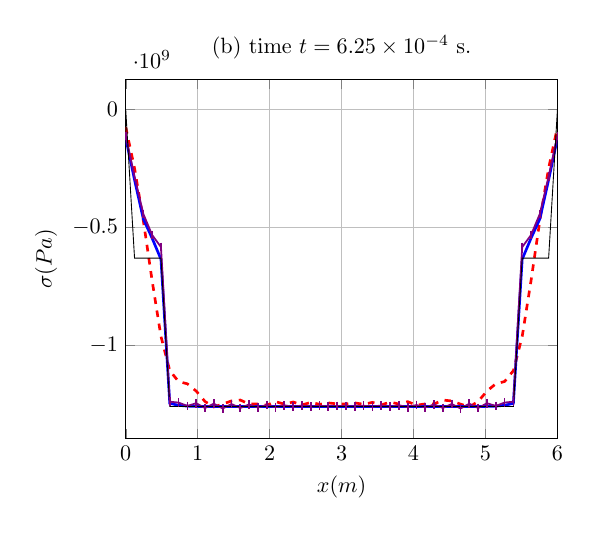
\begin{tikzpicture}[scale=0.8]
\begin{axis}[xlabel=$x (m)$,ylabel=$\sigma (Pa)$,ymajorgrids=true,xmajorgrids=true,legend pos=outer north east,title={(b) time $t = 6.25\times 10^{-4} $ s.},xmin=0.,xmax=6.]
\addplot[Red,very thick,mark=none,dashed] coordinates {(0.0,-74686690.65430246) (0.12244897959183673,-248860978.1693335) (0.24489795918367346,-471505677.3136862) (0.36734693877551017,-727347550.4714894) (0.4897959183673469,-963308331.6520433) (0.6122448979591837,-1108824904.6085515) (0.7346938775510203,-1154837713.915547) (0.8571428571428571,-1164658358.6882505) (0.9795918367346939,-1195327833.6731591) (1.1020408163265305,-1239722495.17177) (1.2244897959183674,-1262625036.5763078) (1.346938775510204,-1250850727.3360605) (1.4693877551020407,-1237335621.1098552) (1.5918367346938775,-1233570784.670482) (1.7142857142857142,-1250022356.590519) (1.836734693877551,-1250064510.2383804) (1.9591836734693877,-1255304260.9119728) (2.0816326530612246,-1240464014.9742188) (2.204081632653061,-1250749408.0219655) (2.326530612244898,-1241771881.0316234) (2.4489795918367347,-1254655253.5739675) (2.571428571428571,-1243386642.1602688) (2.693877551020408,-1251564997.8232079) (2.816326530612245,-1245650942.428049) (2.9387755102040813,-1249901934.3884947) (3.061224489795918,-1249901934.3884926) (3.183673469387755,-1245650942.4280505) (3.306122448979592,-1251564997.8232062) (3.4285714285714284,-1243386642.160271) (3.5510204081632653,-1254655253.5739667) (3.673469387755102,-1241771881.0316243) (3.7959183673469385,-1250749408.0219643) (3.9183673469387754,-1240464014.9742193) (4.040816326530612,-1255304260.911973) (4.163265306122449,-1250064510.238382) (4.285714285714286,-1250022356.59052) (4.408163265306122,-1233570784.670483) (4.530612244897959,-1237335621.1098552) (4.653061224489796,-1250850727.3360612) (4.775510204081632,-1262625036.5763083) (4.8979591836734695,-1239722495.1717708) (5.020408163265306,-1195327833.6731594) (5.142857142857142,-1164658358.688251) (5.26530612244898,-1154837713.915547) (5.387755102040816,-1108824904.6085508) (5.5102040816326525,-963308331.652042) (5.63265306122449,-727347550.4714878) (5.755102040816326,-471505677.3136848) (5.877551020408163,-248860978.16933236) (6.0,-74686690.65430167) };
\addplot[Blue,very thick,mark=none,solid] coordinates {(0.0,-120597397.19248778) (0.12244897959183673,-298539345.15508544) (0.24489795918367346,-464504460.170754) (0.36734693877551017,-546627376.3559334) (0.4897959183673469,-635546108.2543886) (0.6122448979591837,-1247334335.3333962) (0.7346938775510203,-1255980074.5990539) (0.8571428571428571,-1259371705.5275755) (0.9795918367346939,-1260535220.1287405) (1.1020408163265305,-1260885267.5005968) (1.2244897959183674,-1260977777.705495) (1.346938775510204,-1260999265.6570995) (1.4693877551020407,-1261003650.0375175) (1.5918367346938775,-1261004434.5740557) (1.7142857142857142,-1261004557.3391547) (1.836734693877551,-1261004574.0682204) (1.9591836734693877,-1261004576.0419452) (2.0816326530612246,-1261004576.241996) (2.204081632653061,-1261004576.2592359) (2.326530612244898,-1261004576.260481) (2.4489795918367347,-1261004576.260556) (2.571428571428571,-1261004576.2605588) (2.693877551020408,-1261004576.260559) (2.816326530612245,-1261004576.2605588) (2.9387755102040813,-1261004576.260559) (3.061224489795918,-1261004576.2605584) (3.183673469387755,-1261004576.2605586) (3.306122448979592,-1261004576.2605588) (3.4285714285714284,-1261004576.2605581) (3.5510204081632653,-1261004576.2605555) (3.673469387755102,-1261004576.260481) (3.7959183673469385,-1261004576.2592354) (3.9183673469387754,-1261004576.2419953) (4.040816326530612,-1261004576.0419443) (4.163265306122449,-1261004574.06822) (4.285714285714286,-1261004557.3391542) (4.408163265306122,-1261004434.5740552) (4.530612244897959,-1261003650.037517) (4.653061224489796,-1260999265.6570988) (4.775510204081632,-1260977777.7054946) (4.8979591836734695,-1260885267.500596) (5.020408163265306,-1260535220.1287398) (5.142857142857142,-1259371705.5275738) (5.26530612244898,-1255980074.5990536) (5.387755102040816,-1247334335.3333952) (5.5102040816326525,-635546108.2543867) (5.63265306122449,-546627376.3559326) (5.755102040816326,-464504460.1707534) (5.877551020408163,-298539345.15508515) (6.0,-120597397.19248791) };
\addplot[Purple,thick,mark=|,solid] coordinates {(0.0,-111808132.50928691) (0.12244897959183673,-283652980.311345) (0.24489795918367346,-443221012.94130766) (0.36734693877551017,-532712483.6212361) (0.4897959183673469,-583780738.0952947) (0.6122448979591837,-1240572116.142149) (0.7346938775510203,-1244261651.762744) (0.8571428571428571,-1258556998.8403206) (0.9795918367346939,-1246923690.2991939) (1.1020408163265305,-1267582002.156853) (1.2244897959183674,-1248919510.011234) (1.346938775510204,-1269351209.0749319) (1.4693877551020407,-1250347534.9609652) (1.5918367346938775,-1267308507.8062203) (1.7142857142857142,-1252234928.1894917) (1.836734693877551,-1265091742.2400982) (1.9591836734693877,-1254542095.0106862) (2.0816326530612246,-1263677501.5970206) (2.204081632653061,-1255669724.044529) (2.326530612244898,-1262623936.670721) (2.4489795918367347,-1256618647.3458264) (2.571428571428571,-1261747368.978006) (2.693877551020408,-1257589986.0890632) (2.816326530612245,-1260580011.675211) (2.9387755102040813,-1258915831.3187945) (3.061224489795918,-1258915831.3187914) (3.183673469387755,-1260580011.6752121) (3.306122448979592,-1257589986.0890625) (3.4285714285714284,-1261747368.9780068) (3.5510204081632653,-1256618647.3458252) (3.673469387755102,-1262623936.6707222) (3.7959183673469385,-1255669724.0445278) (3.9183673469387754,-1263677501.5970201) (4.040816326530612,-1254542095.0106847) (4.163265306122449,-1265091742.2400992) (4.285714285714286,-1252234928.1894906) (4.408163265306122,-1267308507.80622) (4.530612244897959,-1250347534.9609656) (4.653061224489796,-1269351209.0749316) (4.775510204081632,-1248919510.0112329) (4.8979591836734695,-1267582002.1568534) (5.020408163265306,-1246923690.2991939) (5.142857142857142,-1258556998.8403208) (5.26530612244898,-1244261651.7627428) (5.387755102040816,-1240572116.1421485) (5.5102040816326525,-583780738.0952928) (5.63265306122449,-532712483.6212349) (5.755102040816326,-443221012.9413062) (5.877551020408163,-283652980.3113445) (6.0,-111808132.50928625) };
\addplot[black,thin,mark=none,solid] coordinates {(0.0,-0.0) (0.12244897959183673,-630502288.1302795) (0.24489795918367346,-630502288.1302795) (0.36734693877551017,-630502288.1302795) (0.4897959183673469,-630502288.1302795) (0.6122448979591837,-1261004576.260559) (0.7346938775510203,-1261004576.260559) (0.8571428571428571,-1261004576.260559) (0.9795918367346939,-1261004576.260559) (1.1020408163265305,-1261004576.260559) (1.2244897959183674,-1261004576.260559) (1.346938775510204,-1261004576.260559) (1.4693877551020407,-1261004576.260559) (1.5918367346938775,-1261004576.260559) (1.7142857142857142,-1261004576.260559) (1.836734693877551,-1261004576.260559) (1.9591836734693877,-1261004576.260559) (2.0816326530612246,-1261004576.260559) (2.204081632653061,-1261004576.260559) (2.326530612244898,-1261004576.260559) (2.4489795918367347,-1261004576.260559) (2.571428571428571,-1261004576.260559) (2.693877551020408,-1261004576.260559) (2.816326530612245,-1261004576.260559) (2.9387755102040813,-1261004576.260559) (3.061224489795918,-1261004576.260559) (3.183673469387755,-1261004576.260559) (3.306122448979592,-1261004576.260559) (3.4285714285714284,-1261004576.260559) (3.5510204081632653,-1261004576.260559) (3.673469387755102,-1261004576.260559) (3.7959183673469385,-1261004576.260559) (3.9183673469387754,-1261004576.260559) (4.040816326530612,-1261004576.260559) (4.163265306122449,-1261004576.260559) (4.285714285714286,-1261004576.260559) (4.408163265306122,-1261004576.260559) (4.530612244897959,-1261004576.260559) (4.653061224489796,-1261004576.260559) (4.775510204081632,-1261004576.260559) (4.8979591836734695,-1261004576.260559) (5.020408163265306,-1261004576.260559) (5.142857142857142,-1261004576.260559) (5.26530612244898,-1261004576.260559) (5.387755102040816,-1261004576.260559) (5.5102040816326525,-630502288.1302795) (5.63265306122449,-630502288.1302795) (5.755102040816326,-630502288.1302795) (5.877551020408163,-630502288.1302795) (6.0,-0.0) };
%\legend{usl 1ppc,dgmpm 1ppc (ep solver),dgmpm 1ppc (ac solver),exact}
\end{axis}
\end{tikzpicture}
%%% Local Variables:
%%% mode: latex
%%% TeX-master: "../../mainManuscript"
%%% End:
}
  {% \begin{tikzpicture}[scale=0.4]
% \begin{groupplot}[group style={group size=1 by 1,
% ylabels at=edge left, yticklabels at=edge left,horizontal sep=2.ex,
% vertical sep=4ex,xticklabels at=edge bottom,xlabels at=edge bottom},
% ymajorgrids=true,xmajorgrids=true,enlargelimits=0,xmin=0.,xmax=6.,xlabel=$x (m)$,
% axis on top,scale only axis
% ]
% % \nextgroupplot[ylabel=$\sigma (Pa)$,title={$t = 4.17\times 10^{-4} $ s.},ymin=-1.35e9,ymax=56579516.10614197,]
% % \addplot[Blue,solid,mark=x,very thick,mark size=3pt,mark repeat=3] coordinates{(0.0,-3.2561158711216654e-07) (0.12244897959183673,-6.54162606232603e-22) (0.24489795918367346,0.0) (0.36734693877551017,3.2561158711216643e-07) (0.4897959183673469,-4.884173806682499e-07) (0.6122448979591837,-706703995.0062007) (0.7346938775510203,-739923853.3127105) (0.8571428571428571,-818114621.3278772) (0.9795918367346939,-934350667.0858994) (1.1020408163265305,-1056745717.4113452) (1.2244897959183674,-1153785079.176232) (1.346938775510204,-1213891661.9862223) (1.4693877551020407,-1243675875.166416) (1.5918367346938775,-1255667377.4619899) (1.7142857142857142,-1259628756.7765899) (1.836734693877551,-1260708382.472525) (1.9591836734693877,-1260951555.06527) (2.0816326530612246,-1260996741.6987677) (2.204081632653061,-1261003631.246593) (2.326530612244898,-1261004484.7294881) (2.4489795918367347,-1261004569.3136225) (2.571428571428571,-1261004575.8625927) (2.693877551020408,-1261004576.2443771) (2.816326530612245,-1261004576.2601426) (2.9387755102040813,-1261004576.2605536) (3.061224489795918,-1261004576.2605536) (3.183673469387755,-1261004576.2601426) (3.306122448979592,-1261004576.2443776) (3.4285714285714284,-1261004575.862593) (3.5510204081632653,-1261004569.3136227) (3.673469387755102,-1261004484.7294881) (3.7959183673469385,-1261003631.2465928) (3.9183673469387754,-1260996741.6987677) (4.040816326530612,-1260951555.0652697) (4.163265306122449,-1260708382.4725246) (4.285714285714286,-1259628756.7765894) (4.408163265306122,-1255667377.4619899) (4.530612244897959,-1243675875.1664157) (4.653061224489796,-1213891661.9862223) (4.775510204081632,-1153785079.176232) (4.8979591836734695,-1056745717.4113454) (5.020408163265306,-934350667.0858992) (5.142857142857142,-818114621.327877) (5.26530612244898,-739923853.3127109) (5.387755102040816,-706703995.0062011) (5.5102040816326525,-4.884173806682498e-07) (5.63265306122449,0.0) (5.755102040816326,-4.884173806682498e-07) (5.877551020408163,0.0) (6.0,-4.884173806682498e-07) };
% % \addplot[Purple,solid,mark=+,thick,mark size=3pt,mark repeat=3] coordinates{(0.0,-3.2561158711216654e-07) (0.12244897959183673,-6.54162606232603e-22) (0.24489795918367346,0.0) (0.36734693877551017,3.2561158711216643e-07) (0.4897959183673469,-4.884173806682499e-07) (0.6122448979591837,-710637837.2357953) (0.7346938775510203,-747893724.781927) (0.8571428571428571,-827829409.8631966) (0.9795918367346939,-936780409.853217) (1.1020408163265305,-1054073198.2499647) (1.2244897959183674,-1144128439.1849532) (1.346938775510204,-1207925723.6670742) (1.4693877551020407,-1232372577.7948787) (1.5918367346938775,-1254253728.274747) (1.7142857142857142,-1243570946.3490026) (1.836734693877551,-1268139963.2569304) (1.9591836734693877,-1248035262.8872383) (2.0816326530612246,-1268992337.693115) (2.204081632653061,-1251285653.8729925) (2.326530612244898,-1266352346.5241969) (2.4489795918367347,-1253527311.8706975) (2.571428571428571,-1264419055.233534) (2.693877551020408,-1255474245.0991223) (2.816326530612245,-1261578869.0693417) (2.9387755102040813,-1258168698.6750736) (3.061224489795918,-1258168698.6750731) (3.183673469387755,-1261578869.069342) (3.306122448979592,-1255474245.0991209) (3.4285714285714284,-1264419055.233534) (3.5510204081632653,-1253527311.870696) (3.673469387755102,-1266352346.5241973) (3.7959183673469385,-1251285653.8729923) (3.9183673469387754,-1268992337.6931143) (4.040816326530612,-1248035262.8872375) (4.163265306122449,-1268139963.2569308) (4.285714285714286,-1243570946.3490026) (4.408163265306122,-1254253728.2747467) (4.530612244897959,-1232372577.7948787) (4.653061224489796,-1207925723.6670735) (4.775510204081632,-1144128439.1849532) (4.8979591836734695,-1054073198.2499645) (5.020408163265306,-936780409.853217) (5.142857142857142,-827829409.8631967) (5.26530612244898,-747893724.7819276) (5.387755102040816,-710637837.2357956) (5.5102040816326525,-4.884173806682498e-07) (5.63265306122449,0.0) (5.755102040816326,-4.884173806682498e-07) (5.877551020408163,0.0) (6.0,-4.884173806682498e-07) };
% % \addplot[black,solid,mark=none,thin,mark size=3pt,mark repeat=3] coordinates{(0.0,-0.0) (0.12244897959183673,-0.0) (0.24489795918367346,-0.0) (0.36734693877551017,-0.0) (0.4897959183673469,-0.0) (0.6122448979591837,-700000000.0) (0.7346938775510203,-700000000.0) (0.8571428571428571,-700000000.0) (0.9795918367346939,-700000000.0) (1.1020408163265305,-1261004576.260559) (1.2244897959183674,-1261004576.260559) (1.346938775510204,-1261004576.260559) (1.4693877551020407,-1261004576.260559) (1.5918367346938775,-1261004576.260559) (1.7142857142857142,-1261004576.260559) (1.836734693877551,-1261004576.260559) (1.9591836734693877,-1261004576.260559) (2.0816326530612246,-1261004576.260559) (2.204081632653061,-1261004576.260559) (2.326530612244898,-1261004576.260559) (2.4489795918367347,-1261004576.260559) (2.571428571428571,-1261004576.260559) (2.693877551020408,-1261004576.260559) (2.816326530612245,-1261004576.260559) (2.9387755102040813,-1261004576.260559) (3.061224489795918,-1261004576.260559) (3.183673469387755,-1261004576.260559) (3.306122448979592,-1261004576.260559) (3.4285714285714284,-1261004576.260559) (3.5510204081632653,-1261004576.260559) (3.673469387755102,-1261004576.260559) (3.7959183673469385,-1261004576.260559) (3.9183673469387754,-1261004576.260559) (4.040816326530612,-1261004576.260559) (4.163265306122449,-1261004576.260559) (4.285714285714286,-1261004576.260559) (4.408163265306122,-1261004576.260559) (4.530612244897959,-1261004576.260559) (4.653061224489796,-1261004576.260559) (4.775510204081632,-1261004576.260559) (4.8979591836734695,-1261004576.260559) (5.020408163265306,-700000000.0) (5.142857142857142,-700000000.0) (5.26530612244898,-700000000.0) (5.387755102040816,-700000000.0) (5.5102040816326525,-0.0) (5.63265306122449,-0.0) (5.755102040816326,-0.0) (5.877551020408163,-0.0) (6.0,-0.0) };
% \nextgroupplot[ylabel=$\eps^p $,ymin=-0.0021,ymax=0.0,title={Elastic-plastic plane waves}]
% \addplot[Blue,solid,mark=x,very thick,mark size=3pt,mark repeat=3] coordinates{(0.0,0.0) (0.12244897959183673,0.0) (0.24489795918367346,0.0) (0.36734693877551017,0.0) (0.4897959183673469,0.0) (0.6122448979591837,-2.4267855226065594e-05) (0.7346938775510203,-0.00014452073597361284) (0.8571428571428571,-0.0004275642401009131) (0.9795918367346939,-0.0008483282066457896) (1.1020408163265305,-0.0012913872123487611) (1.2244897959183674,-0.001642660920094959) (1.346938775510204,-0.0018602413103573651) (1.4693877551020407,-0.0019680574666657586) (1.5918367346938775,-0.00201146561977191) (1.7142857142857142,-0.002025805454394895) (1.836734693877551,-0.0020297136017104972) (1.9591836734693877,-0.002030593864489664) (2.0816326530612246,-0.002030757436013639) (2.204081632653061,-0.0020307823755532774) (2.326530612244898,-0.002030785465084119) (2.4489795918367347,-0.0020307857712710334) (2.571428571428571,-0.00203078579497771) (2.693877551020408,-0.0020307857963597366) (2.816326530612245,-0.002030785796416807) (2.9387755102040813,-0.002030785796418294) (3.061224489795918,-0.002030785796418294) (3.183673469387755,-0.0020307857964168056) (3.306122448979592,-0.002030785796359739) (3.4285714285714284,-0.0020307857949777124) (3.5510204081632653,-0.002030785771271032) (3.673469387755102,-0.002030785465084119) (3.7959183673469385,-0.002030782375553277) (3.9183673469387754,-0.0020307574360136386) (4.040816326530612,-0.002030593864489664) (4.163265306122449,-0.0020297136017104964) (4.285714285714286,-0.0020258054543948927) (4.408163265306122,-0.002011465619771909) (4.530612244897959,-0.0019680574666657573) (4.653061224489796,-0.0018602413103573651) (4.775510204081632,-0.0016426609200949592) (4.8979591836734695,-0.001291387212348762) (5.020408163265306,-0.0008483282066457893) (5.142857142857142,-0.00042756424010091193) (5.26530612244898,-0.00014452073597361384) (5.387755102040816,-2.4267855226067292e-05) (5.5102040816326525,0.0) (5.63265306122449,0.0) (5.755102040816326,0.0) (5.877551020408163,0.0) (6.0,0.0) };
% \addplot[Purple,solid,mark=+,thick,mark size=3pt,mark repeat=3] coordinates{(0.0,0.0) (0.12244897959183673,0.0) (0.24489795918367346,0.0) (0.36734693877551017,0.0) (0.4897959183673469,0.0) (0.6122448979591837,-3.850800809337606e-05) (0.7346938775510203,-0.00017337094943683953) (0.8571428571428571,-0.00046273089543238553) (0.9795918367346939,-0.000857123655577256) (1.1020408163265305,-0.0012817129348415013) (1.2244897959183674,-0.0016077047572306) (1.346938775510204,-0.0018386451535459692) (1.4693877551020407,-0.0019271405531036338) (1.5918367346938775,-0.002006348337646142) (1.7142857142857142,-0.002018045326373221) (1.836734693877551,-0.002056615251608797) (1.9591836734693877,-0.0020613216365693464) (2.0816326530612246,-0.002064203896841495) (2.204081632653061,-0.0020644266901542695) (2.326530612244898,-0.0020621094945296272) (2.4489795918367347,-0.002062767607181189) (2.571428571428571,-0.002061489252343496) (2.693877551020408,-0.0020573197208032658) (2.816326530612245,-0.0020502799029179) (2.9387755102040813,-0.0020377776694292327) (3.061224489795918,-0.0020377776694292327) (3.183673469387755,-0.002050279902917899) (3.306122448979592,-0.002057319720803265) (3.4285714285714284,-0.0020614892523434956) (3.5510204081632653,-0.0020627676071811878) (3.673469387755102,-0.0020621094945296285) (3.7959183673469385,-0.0020644266901542695) (3.9183673469387754,-0.0020642038968414953) (4.040816326530612,-0.0020613216365693477) (4.163265306122449,-0.002056615251608799) (4.285714285714286,-0.0020180453263732205) (4.408163265306122,-0.0020063483376461405) (4.530612244897959,-0.0019271405531036334) (4.653061224489796,-0.0018386451535459673) (4.775510204081632,-0.0016077047572305996) (4.8979591836734695,-0.0012817129348415002) (5.020408163265306,-0.0008571236555772557) (5.142857142857142,-0.000462730895432386) (5.26530612244898,-0.0001733709494368422) (5.387755102040816,-3.850800809337776e-05) (5.5102040816326525,0.0) (5.63265306122449,0.0) (5.755102040816326,0.0) (5.877551020408163,0.0) (6.0,0.0) };
% \addplot[black,solid,mark=none,thin,mark size=3pt,mark repeat=3] coordinates{(0.0,-0.0) (0.12244897959183673,-0.0) (0.24489795918367346,-0.0) (0.36734693877551017,-0.0) (0.4897959183673469,-0.0) (0.6122448979591837,-0.0) (0.7346938775510203,-0.0) (0.8571428571428571,-0.0) (0.9795918367346939,-0.0) (1.1020408163265305,-0.002030785796418313) (1.2244897959183674,-0.002030785796418313) (1.346938775510204,-0.002030785796418313) (1.4693877551020407,-0.002030785796418313) (1.5918367346938775,-0.002030785796418313) (1.7142857142857142,-0.002030785796418313) (1.836734693877551,-0.002030785796418313) (1.9591836734693877,-0.002030785796418313) (2.0816326530612246,-0.002030785796418313) (2.204081632653061,-0.002030785796418313) (2.326530612244898,-0.002030785796418313) (2.4489795918367347,-0.002030785796418313) (2.571428571428571,-0.002030785796418313) (2.693877551020408,-0.002030785796418313) (2.816326530612245,-0.002030785796418313) (2.9387755102040813,-0.002030785796418313) (3.061224489795918,-0.002030785796418313) (3.183673469387755,-0.002030785796418313) (3.306122448979592,-0.002030785796418313) (3.4285714285714284,-0.002030785796418313) (3.5510204081632653,-0.002030785796418313) (3.673469387755102,-0.002030785796418313) (3.7959183673469385,-0.002030785796418313) (3.9183673469387754,-0.002030785796418313) (4.040816326530612,-0.002030785796418313) (4.163265306122449,-0.002030785796418313) (4.285714285714286,-0.002030785796418313) (4.408163265306122,-0.002030785796418313) (4.530612244897959,-0.002030785796418313) (4.653061224489796,-0.002030785796418313) (4.775510204081632,-0.002030785796418313) (4.8979591836734695,-0.002030785796418313) (5.020408163265306,-0.0) (5.142857142857142,-0.0) (5.26530612244898,-0.0) (5.387755102040816,-0.0) (5.5102040816326525,-0.0) (5.63265306122449,-0.0) (5.755102040816326,-0.0) (5.877551020408163,-0.0) (6.0,-0.0) };

% \addlegendentry{fvm (elastic-plastic Riemann solver)}
% \addlegendentry{fvm (elastic Riemann solver)}
% \addlegendentry{exact}

% \end{groupplot}
% \end{tikzpicture}


\begin{tikzpicture}[spy using outlines={rectangle, magnification=2, size=.15cm, connect spies},scale=0.6]
\begin{axis}[xlabel=$x \:(\text{m})$,ylabel=$\eps^p $,ymajorgrids=true,xmajorgrids=true,legend pos=north east,title={Plastic waves},xmin=0.,xmax=6.,ymin=-0.0021,ymax=0.00001]
\addplot[Blue,solid,mark=x,very thick,mark size=3pt,mark repeat=3] coordinates{(0.0,0.0) (0.12244897959183673,0.0) (0.24489795918367346,0.0) (0.36734693877551017,0.0) (0.4897959183673469,0.0) (0.6122448979591837,-2.4267855226065594e-05) (0.7346938775510203,-0.00014452073597361284) (0.8571428571428571,-0.0004275642401009131) (0.9795918367346939,-0.0008483282066457896) (1.1020408163265305,-0.0012913872123487611) (1.2244897959183674,-0.001642660920094959) (1.346938775510204,-0.0018602413103573651) (1.4693877551020407,-0.0019680574666657586) (1.5918367346938775,-0.00201146561977191) (1.7142857142857142,-0.002025805454394895) (1.836734693877551,-0.0020297136017104972) (1.9591836734693877,-0.002030593864489664) (2.0816326530612246,-0.002030757436013639) (2.204081632653061,-0.0020307823755532774) (2.326530612244898,-0.002030785465084119) (2.4489795918367347,-0.0020307857712710334) (2.571428571428571,-0.00203078579497771) (2.693877551020408,-0.0020307857963597366) (2.816326530612245,-0.002030785796416807) (2.9387755102040813,-0.002030785796418294) (3.061224489795918,-0.002030785796418294) (3.183673469387755,-0.0020307857964168056) (3.306122448979592,-0.002030785796359739) (3.4285714285714284,-0.0020307857949777124) (3.5510204081632653,-0.002030785771271032) (3.673469387755102,-0.002030785465084119) (3.7959183673469385,-0.002030782375553277) (3.9183673469387754,-0.0020307574360136386) (4.040816326530612,-0.002030593864489664) (4.163265306122449,-0.0020297136017104964) (4.285714285714286,-0.0020258054543948927) (4.408163265306122,-0.002011465619771909) (4.530612244897959,-0.0019680574666657573) (4.653061224489796,-0.0018602413103573651) (4.775510204081632,-0.0016426609200949592) (4.8979591836734695,-0.001291387212348762) (5.020408163265306,-0.0008483282066457893) (5.142857142857142,-0.00042756424010091193) (5.26530612244898,-0.00014452073597361384) (5.387755102040816,-2.4267855226067292e-05) (5.5102040816326525,0.0) (5.63265306122449,0.0) (5.755102040816326,0.0) (5.877551020408163,0.0) (6.0,0.0) };
\addplot[Red,solid,mark=+,very thick,mark size=3pt,mark repeat=3] coordinates{(0.0,0.0) (0.12244897959183673,0.0) (0.24489795918367346,0.0) (0.36734693877551017,0.0) (0.4897959183673469,0.0) (0.6122448979591837,-3.850800809337606e-05) (0.7346938775510203,-0.00017337094943683953) (0.8571428571428571,-0.00046273089543238553) (0.9795918367346939,-0.000857123655577256) (1.1020408163265305,-0.0012817129348415013) (1.2244897959183674,-0.0016077047572306) (1.346938775510204,-0.0018386451535459692) (1.4693877551020407,-0.0019271405531036338) (1.5918367346938775,-0.002006348337646142) (1.7142857142857142,-0.002018045326373221) (1.836734693877551,-0.002056615251608797) (1.9591836734693877,-0.0020613216365693464) (2.0816326530612246,-0.002064203896841495) (2.204081632653061,-0.0020644266901542695) (2.326530612244898,-0.0020621094945296272) (2.4489795918367347,-0.002062767607181189) (2.571428571428571,-0.002061489252343496) (2.693877551020408,-0.0020573197208032658) (2.816326530612245,-0.0020502799029179) (2.9387755102040813,-0.0020377776694292327) (3.061224489795918,-0.0020377776694292327) (3.183673469387755,-0.002050279902917899) (3.306122448979592,-0.002057319720803265) (3.4285714285714284,-0.0020614892523434956) (3.5510204081632653,-0.0020627676071811878) (3.673469387755102,-0.0020621094945296285) (3.7959183673469385,-0.0020644266901542695) (3.9183673469387754,-0.0020642038968414953) (4.040816326530612,-0.0020613216365693477) (4.163265306122449,-0.002056615251608799) (4.285714285714286,-0.0020180453263732205) (4.408163265306122,-0.0020063483376461405) (4.530612244897959,-0.0019271405531036334) (4.653061224489796,-0.0018386451535459673) (4.775510204081632,-0.0016077047572305996) (4.8979591836734695,-0.0012817129348415002) (5.020408163265306,-0.0008571236555772557) (5.142857142857142,-0.000462730895432386) (5.26530612244898,-0.0001733709494368422) (5.387755102040816,-3.850800809337776e-05) (5.5102040816326525,0.0) (5.63265306122449,0.0) (5.755102040816326,0.0) (5.877551020408163,0.0) (6.0,0.0) };
\addplot[black,solid,mark=none,thick,mark size=3pt,mark repeat=3] coordinates{(0.0,-0.0) (0.12244897959183673,-0.0) (0.24489795918367346,-0.0) (0.36734693877551017,-0.0) (0.4897959183673469,-0.0) (0.6122448979591837,-0.0) (0.7346938775510203,-0.0) (0.8571428571428571,-0.0) (0.9795918367346939,-0.0) (1.1020408163265305,-0.002030785796418313) (1.2244897959183674,-0.002030785796418313) (1.346938775510204,-0.002030785796418313) (1.4693877551020407,-0.002030785796418313) (1.5918367346938775,-0.002030785796418313) (1.7142857142857142,-0.002030785796418313) (1.836734693877551,-0.002030785796418313) (1.9591836734693877,-0.002030785796418313) (2.0816326530612246,-0.002030785796418313) (2.204081632653061,-0.002030785796418313) (2.326530612244898,-0.002030785796418313) (2.4489795918367347,-0.002030785796418313) (2.571428571428571,-0.002030785796418313) (2.693877551020408,-0.002030785796418313) (2.816326530612245,-0.002030785796418313) (2.9387755102040813,-0.002030785796418313) (3.061224489795918,-0.002030785796418313) (3.183673469387755,-0.002030785796418313) (3.306122448979592,-0.002030785796418313) (3.4285714285714284,-0.002030785796418313) (3.5510204081632653,-0.002030785796418313) (3.673469387755102,-0.002030785796418313) (3.7959183673469385,-0.002030785796418313) (3.9183673469387754,-0.002030785796418313) (4.040816326530612,-0.002030785796418313) (4.163265306122449,-0.002030785796418313) (4.285714285714286,-0.002030785796418313) (4.408163265306122,-0.002030785796418313) (4.530612244897959,-0.002030785796418313) (4.653061224489796,-0.002030785796418313) (4.775510204081632,-0.002030785796418313) (4.8979591836734695,-0.002030785796418313) (5.020408163265306,-0.0) (5.142857142857142,-0.0) (5.26530612244898,-0.0) (5.387755102040816,-0.0) (5.5102040816326525,-0.0) (5.63265306122449,-0.0) (5.755102040816326,-0.0) (5.877551020408163,-0.0) (6.0,-0.0) };
\begin{scope}
\spy[black,size=1.5cm] on (1.25,0.3) in node [fill=none] at (3.5,2.7);
\end{scope}

\legend{fvm ("elastic" fluxes),fvm ("elastic-plastic" fluxes),exact}
\end{axis}
\end{tikzpicture}
%%% Local Variables:
%%% mode: latex
%%% TeX-master: "../../presentation"
%%% End:
}
  \caption{elastic-plastic RP stress (1ppc)}
  \label{fig:stress_elastoplastic_RP}
\end{figure}
% \begin{figure}[h!]
%   \centering
%   {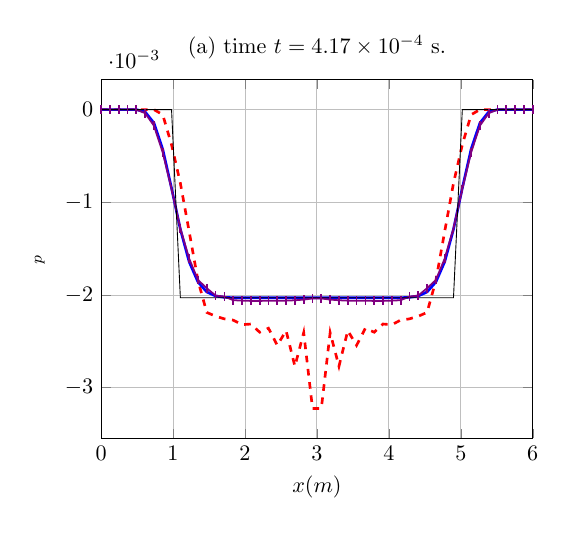
\begin{tikzpicture}[scale=0.8]
\begin{axis}[xlabel=$x (m)$,ylabel=$\eps^p$,ymajorgrids=true,xmajorgrids=true,legend pos=outer north east,title={(a) time $t = 4.17\times 10^{-4} $ s.},xmin=0.,xmax=6.]
\addplot[Red,very thick,mark=none,dashed] coordinates {(0.0,0.0) (0.12244897959183673,0.0) (0.24489795918367346,0.0) (0.36734693877551017,0.0) (0.4897959183673469,0.0) (0.6122448979591837,0.0) (0.7346938775510203,0.0) (0.8571428571428571,-5.5177825258810104e-05) (0.9795918367346939,-0.0003791196239632164) (1.1020408163265305,-0.0007942218458547296) (1.2244897959183674,-0.0013158519965027296) (1.346938775510204,-0.0018458090676901286) (1.4693877551020407,-0.002188794617508559) (1.5918367346938775,-0.002229697455331896) (1.7142857142857142,-0.002258121963594508) (1.836734693877551,-0.002271799079674154) (1.9591836734693877,-0.002320613632318322) (2.0816326530612246,-0.002313868472160546) (2.204081632653061,-0.0024020122032007017) (2.326530612244898,-0.0023588630990294623) (2.4489795918367347,-0.0025433455597807667) (2.571428571428571,-0.002385435935351422) (2.693877551020408,-0.0027693350417516906) (2.816326530612245,-0.0024065265204776445) (2.9387755102040813,-0.0032250612006492966) (3.061224489795918,-0.0032250612006492524) (3.183673469387755,-0.002406526520477666) (3.306122448979592,-0.0027693350417516823) (3.4285714285714284,-0.0023854359353514295) (3.5510204081632653,-0.0025433455597807628) (3.673469387755102,-0.002358863099029464) (3.7959183673469385,-0.0024020122032006983) (3.9183673469387754,-0.0023138684721605448) (4.040816326530612,-0.002320613632318319) (4.163265306122449,-0.0022717990796741546) (4.285714285714286,-0.0022581219635945077) (4.408163265306122,-0.0022296974553318956) (4.530612244897959,-0.0021887946175085595) (4.653061224489796,-0.001845809067690125) (4.775510204081632,-0.0013158519965027254) (4.8979591836734695,-0.0007942218458547295) (5.020408163265306,-0.0003791196239632123) (5.142857142857142,-5.5177825258808404e-05) (5.26530612244898,0.0) (5.387755102040816,0.0) (5.5102040816326525,0.0) (5.63265306122449,0.0) (5.755102040816326,0.0) (5.877551020408163,0.0) (6.0,0.0) };
\addplot[Blue,very thick,mark=none,solid] coordinates {(0.0,0.0) (0.12244897959183673,0.0) (0.24489795918367346,0.0) (0.36734693877551017,0.0) (0.4897959183673469,0.0) (0.6122448979591837,-2.4267855226065594e-05) (0.7346938775510203,-0.00014452073597361284) (0.8571428571428571,-0.0004275642401009131) (0.9795918367346939,-0.0008483282066457896) (1.1020408163265305,-0.0012913872123487611) (1.2244897959183674,-0.001642660920094959) (1.346938775510204,-0.0018602413103573651) (1.4693877551020407,-0.0019680574666657586) (1.5918367346938775,-0.00201146561977191) (1.7142857142857142,-0.002025805454394895) (1.836734693877551,-0.0020297136017104972) (1.9591836734693877,-0.002030593864489664) (2.0816326530612246,-0.002030757436013639) (2.204081632653061,-0.0020307823755532774) (2.326530612244898,-0.002030785465084119) (2.4489795918367347,-0.0020307857712710334) (2.571428571428571,-0.00203078579497771) (2.693877551020408,-0.0020307857963597366) (2.816326530612245,-0.002030785796416807) (2.9387755102040813,-0.002030785796418294) (3.061224489795918,-0.002030785796418294) (3.183673469387755,-0.0020307857964168056) (3.306122448979592,-0.002030785796359739) (3.4285714285714284,-0.0020307857949777124) (3.5510204081632653,-0.002030785771271032) (3.673469387755102,-0.002030785465084119) (3.7959183673469385,-0.002030782375553277) (3.9183673469387754,-0.0020307574360136386) (4.040816326530612,-0.002030593864489664) (4.163265306122449,-0.0020297136017104964) (4.285714285714286,-0.0020258054543948927) (4.408163265306122,-0.002011465619771909) (4.530612244897959,-0.0019680574666657573) (4.653061224489796,-0.0018602413103573651) (4.775510204081632,-0.0016426609200949592) (4.8979591836734695,-0.001291387212348762) (5.020408163265306,-0.0008483282066457893) (5.142857142857142,-0.00042756424010091193) (5.26530612244898,-0.00014452073597361384) (5.387755102040816,-2.4267855226067292e-05) (5.5102040816326525,0.0) (5.63265306122449,0.0) (5.755102040816326,0.0) (5.877551020408163,0.0) (6.0,0.0) };
\addplot[Purple,thick,mark=|,solid] coordinates {(0.0,0.0) (0.12244897959183673,0.0) (0.24489795918367346,0.0) (0.36734693877551017,0.0) (0.4897959183673469,0.0) (0.6122448979591837,-3.850800809337606e-05) (0.7346938775510203,-0.00017337094943683953) (0.8571428571428571,-0.00046273089543238553) (0.9795918367346939,-0.000857123655577256) (1.1020408163265305,-0.0012817129348415013) (1.2244897959183674,-0.0016077047572306) (1.346938775510204,-0.0018386451535459692) (1.4693877551020407,-0.0019271405531036338) (1.5918367346938775,-0.002006348337646142) (1.7142857142857142,-0.002018045326373221) (1.836734693877551,-0.002056615251608797) (1.9591836734693877,-0.0020613216365693464) (2.0816326530612246,-0.002064203896841495) (2.204081632653061,-0.0020644266901542695) (2.326530612244898,-0.0020621094945296272) (2.4489795918367347,-0.002062767607181189) (2.571428571428571,-0.002061489252343496) (2.693877551020408,-0.0020573197208032658) (2.816326530612245,-0.0020502799029179) (2.9387755102040813,-0.0020377776694292327) (3.061224489795918,-0.0020377776694292327) (3.183673469387755,-0.002050279902917899) (3.306122448979592,-0.002057319720803265) (3.4285714285714284,-0.0020614892523434956) (3.5510204081632653,-0.0020627676071811878) (3.673469387755102,-0.0020621094945296285) (3.7959183673469385,-0.0020644266901542695) (3.9183673469387754,-0.0020642038968414953) (4.040816326530612,-0.0020613216365693477) (4.163265306122449,-0.002056615251608799) (4.285714285714286,-0.0020180453263732205) (4.408163265306122,-0.0020063483376461405) (4.530612244897959,-0.0019271405531036334) (4.653061224489796,-0.0018386451535459673) (4.775510204081632,-0.0016077047572305996) (4.8979591836734695,-0.0012817129348415002) (5.020408163265306,-0.0008571236555772557) (5.142857142857142,-0.000462730895432386) (5.26530612244898,-0.0001733709494368422) (5.387755102040816,-3.850800809337776e-05) (5.5102040816326525,0.0) (5.63265306122449,0.0) (5.755102040816326,0.0) (5.877551020408163,0.0) (6.0,0.0) };
\addplot[black,thin,mark=none,solid] coordinates {(0.0,-0.0) (0.12244897959183673,-0.0) (0.24489795918367346,-0.0) (0.36734693877551017,-0.0) (0.4897959183673469,-0.0) (0.6122448979591837,-0.0) (0.7346938775510203,-0.0) (0.8571428571428571,-0.0) (0.9795918367346939,-0.0) (1.1020408163265305,-0.002030785796418313) (1.2244897959183674,-0.002030785796418313) (1.346938775510204,-0.002030785796418313) (1.4693877551020407,-0.002030785796418313) (1.5918367346938775,-0.002030785796418313) (1.7142857142857142,-0.002030785796418313) (1.836734693877551,-0.002030785796418313) (1.9591836734693877,-0.002030785796418313) (2.0816326530612246,-0.002030785796418313) (2.204081632653061,-0.002030785796418313) (2.326530612244898,-0.002030785796418313) (2.4489795918367347,-0.002030785796418313) (2.571428571428571,-0.002030785796418313) (2.693877551020408,-0.002030785796418313) (2.816326530612245,-0.002030785796418313) (2.9387755102040813,-0.002030785796418313) (3.061224489795918,-0.002030785796418313) (3.183673469387755,-0.002030785796418313) (3.306122448979592,-0.002030785796418313) (3.4285714285714284,-0.002030785796418313) (3.5510204081632653,-0.002030785796418313) (3.673469387755102,-0.002030785796418313) (3.7959183673469385,-0.002030785796418313) (3.9183673469387754,-0.002030785796418313) (4.040816326530612,-0.002030785796418313) (4.163265306122449,-0.002030785796418313) (4.285714285714286,-0.002030785796418313) (4.408163265306122,-0.002030785796418313) (4.530612244897959,-0.002030785796418313) (4.653061224489796,-0.002030785796418313) (4.775510204081632,-0.002030785796418313) (4.8979591836734695,-0.002030785796418313) (5.020408163265306,-0.0) (5.142857142857142,-0.0) (5.26530612244898,-0.0) (5.387755102040816,-0.0) (5.5102040816326525,-0.0) (5.63265306122449,-0.0) (5.755102040816326,-0.0) (5.877551020408163,-0.0) (6.0,-0.0) };
%\legend{usl 1ppc,dgmpm 1ppc (ep solver),dgmpm 1ppc (ac solver),exact}
\end{axis}
\end{tikzpicture}
%%% Local Variables:
%%% mode: latex
%%% TeX-master: "../../mainManuscript"
%%% End:
}
%   {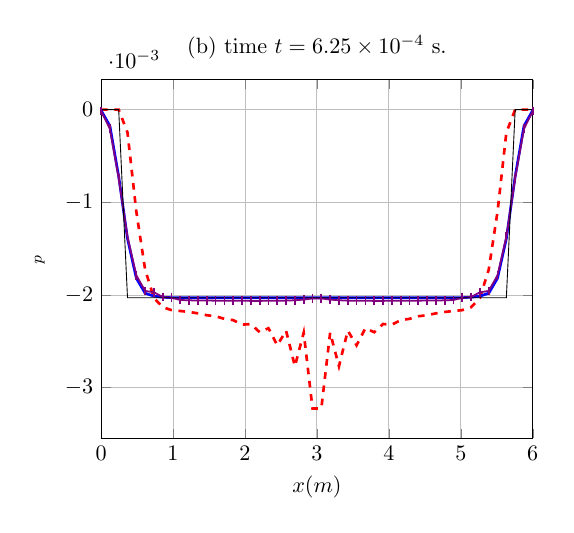
\begin{tikzpicture}[scale=0.8]
\begin{axis}[xlabel=$x (m)$,ylabel=$\eps^p$,ymajorgrids=true,xmajorgrids=true,legend pos=outer north east,title={(b) time $t = 6.25\times 10^{-4} $ s.},xmin=0.,xmax=6.]
\addplot[Red,very thick,mark=none,dashed] coordinates {(0.0,0.0) (0.12244897959183673,0.0) (0.24489795918367346,0.0) (0.36734693877551017,-0.0002478348228815541) (0.4897959183673469,-0.0011004378155012712) (0.6122448979591837,-0.0017260409269248597) (0.7346938775510203,-0.002031865332982762) (0.8571428571428571,-0.002132968518977378) (0.9795918367346939,-0.0021636018350532395) (1.1020408163265305,-0.0021733079916121177) (1.2244897959183674,-0.00218350748748031) (1.346938775510204,-0.002198645448466017) (1.4693877551020407,-0.002218920213241705) (1.5918367346938775,-0.002229697455331896) (1.7142857142857142,-0.002258121963594508) (1.836734693877551,-0.002271799079674154) (1.9591836734693877,-0.002320613632318322) (2.0816326530612246,-0.002313868472160546) (2.204081632653061,-0.0024020122032007017) (2.326530612244898,-0.0023588630990294623) (2.4489795918367347,-0.0025433455597807667) (2.571428571428571,-0.002385435935351422) (2.693877551020408,-0.0027693350417516906) (2.816326530612245,-0.0024065265204776445) (2.9387755102040813,-0.0032250612006492966) (3.061224489795918,-0.0032250612006492524) (3.183673469387755,-0.002406526520477666) (3.306122448979592,-0.0027693350417516823) (3.4285714285714284,-0.0023854359353514295) (3.5510204081632653,-0.0025433455597807628) (3.673469387755102,-0.002358863099029464) (3.7959183673469385,-0.0024020122032006983) (3.9183673469387754,-0.0023138684721605448) (4.040816326530612,-0.002320613632318319) (4.163265306122449,-0.0022717990796741546) (4.285714285714286,-0.0022581219635945077) (4.408163265306122,-0.0022296974553318956) (4.530612244897959,-0.0022189202132417056) (4.653061224489796,-0.0021986454484660173) (4.775510204081632,-0.0021835074874803095) (4.8979591836734695,-0.0021733079916121186) (5.020408163265306,-0.0021636018350532395) (5.142857142857142,-0.002132968518977378) (5.26530612244898,-0.002031865332982763) (5.387755102040816,-0.0017260409269248577) (5.5102040816326525,-0.0011004378155012658) (5.63265306122449,-0.0002478348228815494) (5.755102040816326,0.0) (5.877551020408163,0.0) (6.0,0.0) };
\addplot[Blue,very thick,mark=none,solid] coordinates {(0.0,-8.02367288935203e-06) (0.12244897959183673,-0.00017614426387335805) (0.24489795918367346,-0.0007207542691858686) (0.36734693877551017,-0.0013919930410856215) (0.4897959183673469,-0.001818355598439618) (0.6122448979591837,-0.001981300761387861) (0.7346938775510203,-0.0020125975551096974) (0.8571428571428571,-0.002024874952136019) (0.9795918367346939,-0.0020290867696967987) (1.1020408163265305,-0.002030353909504423) (1.2244897959183674,-0.0020306887880741907) (1.346938775510204,-0.0020307665725143873) (1.4693877551020407,-0.0020307824435747243) (1.5918367346938775,-0.0020307852835259937) (1.7142857142857142,-0.0020307857279245408) (1.836734693877551,-0.0020307857884822454) (1.9591836734693877,-0.00203078579562695) (2.0816326530612246,-0.002030785796351117) (2.204081632653061,-0.0020307857964135248) (2.326530612244898,-0.002030785796418031) (2.4489795918367347,-0.002030785796418302) (2.571428571428571,-0.0020307857964183135) (2.693877551020408,-0.002030785796418313) (2.816326530612245,-0.002030785796418313) (2.9387755102040813,-0.002030785796418314) (3.061224489795918,-0.0020307857964183135) (3.183673469387755,-0.0020307857964183135) (3.306122448979592,-0.0020307857964183126) (3.4285714285714284,-0.0020307857964183113) (3.5510204081632653,-0.0020307857964183005) (3.673469387755102,-0.002030785796418031) (3.7959183673469385,-0.0020307857964135217) (3.9183673469387754,-0.0020307857963511138) (4.040816326530612,-0.002030785795626948) (4.163265306122449,-0.0020307857884822433) (4.285714285714286,-0.0020307857279245403) (4.408163265306122,-0.0020307852835259915) (4.530612244897959,-0.0020307824435747226) (4.653061224489796,-0.0020307665725143842) (4.775510204081632,-0.002030688788074188) (4.8979591836734695,-0.0020303539095044196) (5.020408163265306,-0.0020290867696967953) (5.142857142857142,-0.0020248749521360144) (5.26530612244898,-0.0020125975551096966) (5.387755102040816,-0.0019813007613878565) (5.5102040816326525,-0.0018183555984396154) (5.63265306122449,-0.0013919930410856195) (5.755102040816326,-0.0007207542691858678) (5.877551020408163,-0.0001761442638733595) (6.0,-8.023672889353243e-06) };
\addplot[Purple,thick,mark=|,solid] coordinates {(0.0,-1.4376766038990375e-05) (0.12244897959183673,-0.0002078915703532438) (0.24489795918367346,-0.000740641579521879) (0.36734693877551017,-0.0013729886129224668) (0.4897959183673469,-0.001786873759629078) (0.6122448979591837,-0.0019568221398810824) (0.7346938775510203,-0.0019710253863315036) (0.8571428571428571,-0.002021925787657269) (0.9795918367346939,-0.00203043998544926) (1.1020408163265305,-0.002054595482920735) (1.2244897959183674,-0.0020576351166755064) (1.346938775510204,-0.0020609998518549564) (1.4693877551020407,-0.0020606031772355433) (1.5918367346938775,-0.002061501114574304) (1.7142857142857142,-0.002061887903336271) (1.836734693877551,-0.002062455598454706) (1.9591836734693877,-0.0020617923316583004) (2.0816326530612246,-0.002064203896841495) (2.204081632653061,-0.0020644266901542695) (2.326530612244898,-0.0020621094945296272) (2.4489795918367347,-0.002062767607181189) (2.571428571428571,-0.002061489252343496) (2.693877551020408,-0.0020573197208032658) (2.816326530612245,-0.0020502799029179) (2.9387755102040813,-0.0020377776694292327) (3.061224489795918,-0.0020377776694292327) (3.183673469387755,-0.002050279902917899) (3.306122448979592,-0.002057319720803265) (3.4285714285714284,-0.0020614892523434956) (3.5510204081632653,-0.0020627676071811878) (3.673469387755102,-0.0020621094945296285) (3.7959183673469385,-0.0020644266901542695) (3.9183673469387754,-0.0020642038968414953) (4.040816326530612,-0.0020617923316583004) (4.163265306122449,-0.002062455598454705) (4.285714285714286,-0.0020618879033362705) (4.408163265306122,-0.002061501114574307) (4.530612244897959,-0.0020606031772355464) (4.653061224489796,-0.002060999851854956) (4.775510204081632,-0.002057635116675507) (4.8979591836734695,-0.002054595482920736) (5.020408163265306,-0.002030439985449261) (5.142857142857142,-0.0020219257876572696) (5.26530612244898,-0.001971025386331503) (5.387755102040816,-0.0019568221398810802) (5.5102040816326525,-0.0017868737596290767) (5.63265306122449,-0.0013729886129224679) (5.755102040816326,-0.0007406415795218811) (5.877551020408163,-0.00020789157035324622) (6.0,-1.4376766038991588e-05) };
\addplot[black,thin,mark=none,solid] coordinates {(0.0,-0.0) (0.12244897959183673,-0.0) (0.24489795918367346,-0.0) (0.36734693877551017,-0.002030785796418313) (0.4897959183673469,-0.002030785796418313) (0.6122448979591837,-0.002030785796418313) (0.7346938775510203,-0.002030785796418313) (0.8571428571428571,-0.002030785796418313) (0.9795918367346939,-0.002030785796418313) (1.1020408163265305,-0.002030785796418313) (1.2244897959183674,-0.002030785796418313) (1.346938775510204,-0.002030785796418313) (1.4693877551020407,-0.002030785796418313) (1.5918367346938775,-0.002030785796418313) (1.7142857142857142,-0.002030785796418313) (1.836734693877551,-0.002030785796418313) (1.9591836734693877,-0.002030785796418313) (2.0816326530612246,-0.002030785796418313) (2.204081632653061,-0.002030785796418313) (2.326530612244898,-0.002030785796418313) (2.4489795918367347,-0.002030785796418313) (2.571428571428571,-0.002030785796418313) (2.693877551020408,-0.002030785796418313) (2.816326530612245,-0.002030785796418313) (2.9387755102040813,-0.002030785796418313) (3.061224489795918,-0.002030785796418313) (3.183673469387755,-0.002030785796418313) (3.306122448979592,-0.002030785796418313) (3.4285714285714284,-0.002030785796418313) (3.5510204081632653,-0.002030785796418313) (3.673469387755102,-0.002030785796418313) (3.7959183673469385,-0.002030785796418313) (3.9183673469387754,-0.002030785796418313) (4.040816326530612,-0.002030785796418313) (4.163265306122449,-0.002030785796418313) (4.285714285714286,-0.002030785796418313) (4.408163265306122,-0.002030785796418313) (4.530612244897959,-0.002030785796418313) (4.653061224489796,-0.002030785796418313) (4.775510204081632,-0.002030785796418313) (4.8979591836734695,-0.002030785796418313) (5.020408163265306,-0.002030785796418313) (5.142857142857142,-0.002030785796418313) (5.26530612244898,-0.002030785796418313) (5.387755102040816,-0.002030785796418313) (5.5102040816326525,-0.002030785796418313) (5.63265306122449,-0.002030785796418313) (5.755102040816326,-0.0) (5.877551020408163,-0.0) (6.0,-0.0) };
%\legend{usl 1ppc,dgmpm 1ppc (ep solver),dgmpm 1ppc (ac solver),exact}
\end{axis}
\end{tikzpicture}
%%% Local Variables:
%%% mode: latex
%%% TeX-master: "../../mainManuscript"
%%% End:
}
%   {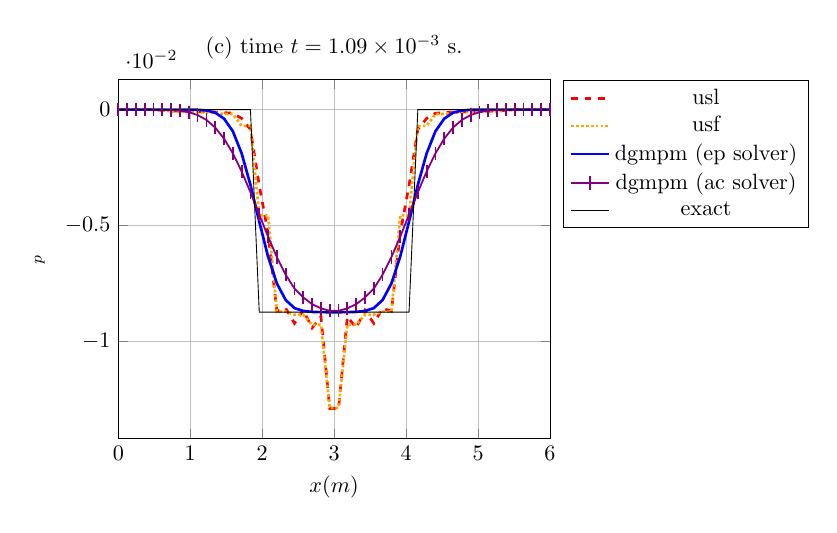
\begin{tikzpicture}[scale=0.8]
\begin{axis}[xlabel=$x (m)$,ylabel=$\eps^p$,ymajorgrids=true,xmajorgrids=true,legend pos=outer north east,title={(c) time $t = 1.09\times 10^{-3} $ s.},xmin=0.,xmax=6.]
\addplot[Red,very thick,mark=none,dashed,mark size=3pt] coordinates {(0.0,0.0) (0.12244897959183673,0.0) (0.24489795918367346,0.0) (0.36734693877551017,0.0) (0.4897959183673469,0.0) (0.6122448979591837,-3.577487902203997e-05) (0.7346938775510203,-6.306588245633642e-05) (0.8571428571428571,-6.949496312549484e-05) (0.9795918367346939,-8.005219978840035e-05) (1.1020408163265305,-9.009475914811774e-05) (1.2244897959183674,-9.858795071160678e-05) (1.346938775510204,-0.00010648019894997112) (1.4693877551020407,-0.00013090237763271645) (1.5918367346938775,-0.00015585484694440393) (1.7142857142857142,-0.00037807434010367157) (1.836734693877551,-0.0008542508721889013) (1.9591836734693877,-0.003265580636192999) (2.0816326530612246,-0.005332403663610279) (2.204081632653061,-0.008685547798871193) (2.326530612244898,-0.008557827562005196) (2.4489795918367347,-0.009212270529983918) (2.571428571428571,-0.008640321746270047) (2.693877551020408,-0.009408157524816411) (2.816326530612245,-0.008914806029937274) (2.9387755102040813,-0.012877303196726952) (3.061224489795918,-0.012877303196726607) (3.183673469387755,-0.008914806029937388) (3.306122448979592,-0.00940815752481628) (3.4285714285714284,-0.008640321746270135) (3.5510204081632653,-0.009212270529983827) (3.673469387755102,-0.008557827562005267) (3.7959183673469385,-0.008685547798871113) (3.9183673469387754,-0.005332403663610266) (4.040816326530612,-0.003265580636192934) (4.163265306122449,-0.0008542508721888987) (4.285714285714286,-0.00037807434010366447) (4.408163265306122,-0.00015585484694441217) (4.530612244897959,-0.00013090237763272187) (4.653061224489796,-0.00010648019894998299) (4.775510204081632,-9.858795071160708e-05) (4.8979591836734695,-9.00947591481104e-05) (5.020408163265306,-8.005219978840008e-05) (5.142857142857142,-6.949496312550109e-05) (5.26530612244898,-6.306588245633955e-05) (5.387755102040816,-3.5774879022040825e-05) (5.5102040816326525,0.0) (5.63265306122449,0.0) (5.755102040816326,0.0) (5.877551020408163,0.0) (6.0,0.0) };
\addplot[Orange,very thick,mark=none,densely dotted,mark size=3pt] coordinates {(0.0,0.0) (0.12244897959183673,0.0) (0.24489795918367346,0.0) (0.36734693877551017,0.0) (0.4897959183673469,-2.538923006910029e-05) (0.6122448979591837,-2.538923006910313e-05) (0.7346938775510203,-8.244814250531935e-05) (0.8571428571428571,-8.244814250532784e-05) (0.9795918367346939,-9.872933660087075e-05) (1.1020408163265305,-9.872933660088494e-05) (1.2244897959183674,-0.0001315062617808007) (1.346938775510204,-0.00013150626178080356) (1.4693877551020407,-0.00019206486011486058) (1.5918367346938775,-0.00019206486011486164) (1.7142857142857142,-0.0007020520949462637) (1.836734693877551,-0.0007020520949463319) (1.9591836734693877,-0.004555064753072419) (2.0816326530612246,-0.004555064753072378) (2.204081632653061,-0.008705849105597185) (2.326530612244898,-0.008705849105596963) (2.4489795918367347,-0.008835786836669598) (2.571428571428571,-0.008835786836669407) (2.693877551020408,-0.009270316426799752) (2.816326530612245,-0.00927031642679947) (2.9387755102040813,-0.012853848358106693) (3.061224489795918,-0.0128538483581062) (3.183673469387755,-0.009270316426799761) (3.306122448979592,-0.00927031642679946) (3.4285714285714284,-0.008835786836669664) (3.5510204081632653,-0.008835786836669336) (3.673469387755102,-0.008705849105597198) (3.7959183673469385,-0.00870584910559694) (3.9183673469387754,-0.004555064753072482) (4.040816326530612,-0.0045550647530723165) (4.163265306122449,-0.0007020520949462988) (4.285714285714286,-0.0007020520949462926) (4.408163265306122,-0.00019206486011485316) (4.530612244897959,-0.00019206486011487072) (4.653061224489796,-0.00013150626178079844) (4.775510204081632,-0.00013150626178081435) (4.8979591836734695,-9.872933660088637e-05) (5.020408163265306,-9.872933660086991e-05) (5.142857142857142,-8.244814250533099e-05) (5.26530612244898,-8.244814250531593e-05) (5.387755102040816,-2.5389230069104546e-05) (5.5102040816326525,-2.538923006909944e-05) (5.63265306122449,0.0) (5.755102040816326,0.0) (5.877551020408163,0.0) (6.0,0.0) };
\addplot[Blue,very thick,mark=none,solid,mark size=3pt] coordinates {(0.0,-5.676632835751488e-19) (0.12244897959183673,-2.3898624238513766e-16) (0.24489795918367346,-3.735990751357306e-14) (0.36734693877551017,-2.3089144911084856e-12) (0.4897959183673469,-7.596762237094698e-11) (0.6122448979591837,-1.5415975357804979e-09) (0.7346938775510203,-2.1087029002110162e-08) (0.8571428571428571,-2.0628580472526095e-07) (0.9795918367346939,-1.5051975779320511e-06) (1.1020408163265305,-8.452232526292688e-06) (1.2244897959183674,-3.741900938747327e-05) (1.346938775510204,-0.00013315210803806102) (1.4693877551020407,-0.00038701776930482674) (1.5918367346938775,-0.0009319386970470464) (1.7142857142857142,-0.0018842066770200564) (1.836734693877551,-0.0032431409441831516) (1.9591836734693877,-0.004827293901207316) (2.0816326530612246,-0.00633202118341673) (2.204081632653061,-0.007489880430691718) (2.326530612244898,-0.008204526972019307) (2.4489795918367347,-0.008552921390073501) (2.571428571428571,-0.008674876019514461) (2.693877551020408,-0.008716486656783273) (2.816326530612245,-0.008726887116624966) (2.9387755102040813,-0.008728580772745199) (3.061224489795918,-0.008728580772745199) (3.183673469387755,-0.008726887116624966) (3.306122448979592,-0.00871648665678328) (3.4285714285714284,-0.008674876019514466) (3.5510204081632653,-0.008552921390073511) (3.673469387755102,-0.008204526972019318) (3.7959183673469385,-0.007489880430691721) (3.9183673469387754,-0.00633202118341673) (4.040816326530612,-0.0048272939012073204) (4.163265306122449,-0.0032431409441831525) (4.285714285714286,-0.001884206677020053) (4.408163265306122,-0.0009319386970470392) (4.530612244897959,-0.0003870177693048181) (4.653061224489796,-0.0001331521080380519) (4.775510204081632,-3.7419009387462476e-05) (4.8979591836734695,-8.452232526284741e-06) (5.020408163265306,-1.5051975779246716e-06) (5.142857142857142,-2.0628580471617835e-07) (5.26530612244898,-2.1087028991608393e-08) (5.387755102040816,-1.5415975312391917e-09) (5.5102040816326525,-7.596762123562041e-11) (5.63265306122449,-2.308913923445202e-12) (5.755102040816326,-3.7358772187005907e-14) (5.877551020408163,-2.4097306387765065e-16) (6.0,-8.514949253627233e-19) };
\addplot[Purple,thick,mark=|,solid,mark size=3pt] coordinates {(0.0,-3.467385013898214e-10) (0.12244897959183673,-6.644251997414089e-09) (0.24489795918367346,-6.120364582198007e-08) (0.36734693877551017,-3.7004598133932975e-07) (0.4897959183673469,-1.6717102054749217e-06) (0.6122448979591837,-6.0577702267402696e-06) (0.7346938775510203,-1.840911253039241e-05) (0.8571428571428571,-4.835925381669828e-05) (0.9795918367346939,-0.00011223737260040385) (1.1020408163265305,-0.00023395773050929446) (1.2244897959183674,-0.0004436331315934306) (1.346938775510204,-0.0007730984959851503) (1.4693877551020407,-0.0012485859668253667) (1.5918367346938775,-0.0018821633869525222) (1.7142857142857142,-0.002664609061018192) (1.836734693877551,-0.003562529161556987) (1.9591836734693877,-0.004521471661696522) (2.0816326530612246,-0.00547485124057479) (2.204081632653061,-0.0063564357486554195) (2.326530612244898,-0.007112831388334339) (2.4489795918367347,-0.00771240428840972) (2.571428571428571,-0.008095314013503907) (2.693877551020408,-0.008383092819259995) (2.816326530612245,-0.008562083426603865) (2.9387755102040813,-0.008669921749349111) (3.061224489795918,-0.008669921749349111) (3.183673469387755,-0.008562083426603865) (3.306122448979592,-0.008383092819260002) (3.4285714285714284,-0.008095314013503904) (3.5510204081632653,-0.007712404288409718) (3.673469387755102,-0.007112831388334339) (3.7959183673469385,-0.006356435748655418) (3.9183673469387754,-0.005474851240574789) (4.040816326530612,-0.004521471661696523) (4.163265306122449,-0.0035625291615569853) (4.285714285714286,-0.0026646090610181854) (4.408163265306122,-0.0018821633869525133) (4.530612244897959,-0.0012485859668253676) (4.653061224489796,-0.0007730984959851409) (4.775510204081632,-0.00044363313159342715) (4.8979591836734695,-0.00023395773050929625) (5.020408163265306,-0.000112237372600403) (5.142857142857142,-4.8359253816693455e-05) (5.26530612244898,-1.8409112530390706e-05) (5.387755102040816,-6.057770226735445e-06) (5.5102040816326525,-1.6717102054752055e-06) (5.63265306122449,-3.7004598133932975e-07) (5.755102040816326,-6.120364582027707e-08) (5.877551020408163,-6.6442519974140885e-09) (6.0,-3.467385011059897e-10) };
\addplot[black,thin,mark=none,solid,mark size=3pt] coordinates {(0.0,-0.0) (0.12244897959183673,-0.0) (0.24489795918367346,-0.0) (0.36734693877551017,-0.0) (0.4897959183673469,-0.0) (0.6122448979591837,-0.0) (0.7346938775510203,-0.0) (0.8571428571428571,-0.0) (0.9795918367346939,-0.0) (1.1020408163265305,-0.0) (1.2244897959183674,-0.0) (1.346938775510204,-0.0) (1.4693877551020407,-0.0) (1.5918367346938775,-0.0) (1.7142857142857142,-0.0) (1.836734693877551,-0.0) (1.9591836734693877,-0.008728715609439695) (2.0816326530612246,-0.008728715609439695) (2.204081632653061,-0.008728715609439695) (2.326530612244898,-0.008728715609439695) (2.4489795918367347,-0.008728715609439695) (2.571428571428571,-0.008728715609439695) (2.693877551020408,-0.008728715609439695) (2.816326530612245,-0.008728715609439695) (2.9387755102040813,-0.008728715609439695) (3.061224489795918,-0.008728715609439695) (3.183673469387755,-0.008728715609439695) (3.306122448979592,-0.008728715609439695) (3.4285714285714284,-0.008728715609439695) (3.5510204081632653,-0.008728715609439695) (3.673469387755102,-0.008728715609439695) (3.7959183673469385,-0.008728715609439695) (3.9183673469387754,-0.008728715609439695) (4.040816326530612,-0.008728715609439695) (4.163265306122449,-0.0) (4.285714285714286,-0.0) (4.408163265306122,-0.0) (4.530612244897959,-0.0) (4.653061224489796,-0.0) (4.775510204081632,-0.0) (4.8979591836734695,-0.0) (5.020408163265306,-0.0) (5.142857142857142,-0.0) (5.26530612244898,-0.0) (5.387755102040816,-0.0) (5.5102040816326525,-0.0) (5.63265306122449,-0.0) (5.755102040816326,-0.0) (5.877551020408163,-0.0) (6.0,-0.0) };
\legend{usl,usf,dgmpm (ep solver),dgmpm (ac solver),exact}
\end{axis}
\end{tikzpicture}
%%% Local Variables:
%%% mode: latex
%%% TeX-master: "../../mainManuscript"
%%% End:
}
%   \caption{elastic-plastic RP epsp (1ppc)}
%   \label{fig:epsp_elastoplastic_RP}
% \end{figure}
% \begin{figure}[h!]
%   \centering
%   {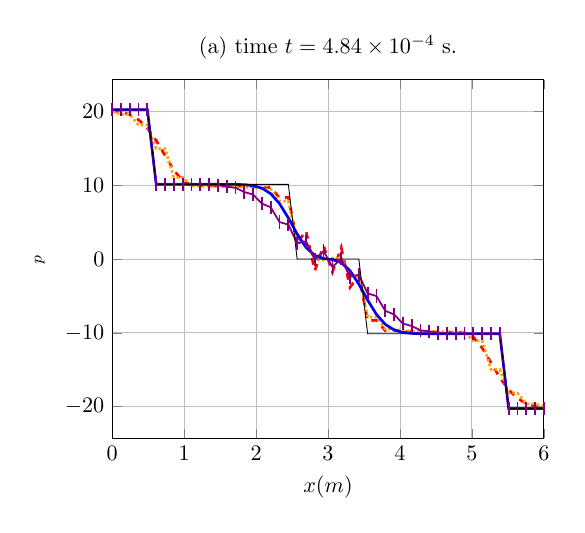
\begin{tikzpicture}[scale=0.8]
\begin{axis}[xlabel=$x (m)$,ylabel=$\eps^p$,ymajorgrids=true,xmajorgrids=true,legend pos=outer north east,title={(a) time $t = 4.84\times 10^{-4} $ s.},xmin=0.,xmax=6.]
\addplot[Red,very thick,mark=none,dashed,mark size=3pt] coordinates {(0.0,20.097963912667037) (0.12244897959183673,19.948200686683876) (0.24489795918367346,19.581623512332886) (0.36734693877551017,18.880401887543975) (0.4897959183673469,17.722027378885375) (0.6122448979591837,16.06462148503811) (0.7346938775510203,14.04922210395701) (0.8571428571428571,12.050777140391757) (0.9795918367346939,10.594448884991046) (1.1020408163265305,10.000299710369095) (1.2244897959183674,9.921016971597252) (1.346938775510204,9.905209334686656) (1.4693877551020407,9.897486036553882) (1.5918367346938775,9.881252793533395) (1.7142857142857142,9.874006895319209) (1.836734693877551,9.827852089496398) (1.9591836734693877,9.84660741015339) (2.0816326530612246,9.635377249359347) (2.204081632653061,9.703660809593103) (2.326530612244898,8.285921376176095) (2.4489795918367347,8.370712342612837) (2.571428571428571,2.1722672846759363) (2.693877551020408,3.830651803002166) (2.816326530612245,-1.5782561078814068) (2.9387755102040813,1.7774061156194738) (3.061224489795918,-1.777406115619491) (3.183673469387755,1.578256107881407) (3.306122448979592,-3.830651803002178) (3.4285714285714284,-2.172267284675949) (3.5510204081632653,-8.370712342612856) (3.673469387755102,-8.285921376176088) (3.7959183673469385,-9.703660809593108) (3.9183673469387754,-9.63537724935935) (4.040816326530612,-9.846607410153386) (4.163265306122449,-9.827852089496393) (4.285714285714286,-9.874006895319202) (4.408163265306122,-9.881252793533392) (4.530612244897959,-9.897486036553879) (4.653061224489796,-9.905209334686653) (4.775510204081632,-9.921016971597266) (4.8979591836734695,-10.000299710369097) (5.020408163265306,-10.594448884991042) (5.142857142857142,-12.05077714039174) (5.26530612244898,-14.049222103957007) (5.387755102040816,-16.064621485038092) (5.5102040816326525,-17.722027378885365) (5.63265306122449,-18.880401887543975) (5.755102040816326,-19.58162351233289) (5.877551020408163,-19.94820068668387) (6.0,-20.09796391266704) };
\addplot[Orange,very thick,mark=none,densely dotted,mark size=3pt] coordinates {(0.0,19.98524356533391) (0.12244897959183673,19.624972673600908) (0.24489795918367346,19.62497267360088) (0.36734693877551017,18.160148281550097) (0.4897959183673469,18.160148281550075) (0.6122448979591837,14.967460990115796) (0.7346938775510203,14.967460990115748) (0.8571428571428571,11.093523181440727) (0.9795918367346939,11.093523181440661) (1.1020408163265305,9.884184161534229) (1.2244897959183674,9.88418416153415) (1.346938775510204,9.848988655347343) (1.4693877551020407,9.848988655347272) (1.5918367346938775,9.805312262992565) (1.7142857142857142,9.805312262992501) (1.836734693877551,9.73354264540347) (1.9591836734693877,9.733542645403414) (2.0816326530612246,9.471881937395924) (2.204081632653061,9.471881937395832) (2.326530612244898,7.860641714627962) (2.4489795918367347,7.860641714627863) (2.571428571428571,2.220437432310992) (2.693877551020408,2.220437432310934) (2.816326530612245,-0.12736436093351383) (2.9387755102040813,-0.1273643609335115) (3.061224489795918,0.12736436093352144) (3.183673469387755,0.12736436093350467) (3.306122448979592,-2.220437432310998) (3.4285714285714284,-2.220437432310941) (3.5510204081632653,-7.860641714628002) (3.673469387755102,-7.860641714627828) (3.7959183673469385,-9.47188193739596) (3.9183673469387754,-9.471881937395791) (4.040816326530612,-9.733542645403523) (4.163265306122449,-9.73354264540336) (4.285714285714286,-9.805312262992585) (4.408163265306122,-9.805312262992468) (4.530612244897959,-9.848988655347373) (4.653061224489796,-9.848988655347233) (4.775510204081632,-9.884184161534241) (4.8979591836734695,-9.884184161534145) (5.020408163265306,-11.093523181440743) (5.142857142857142,-11.093523181440638) (5.26530612244898,-14.967460990115821) (5.387755102040816,-14.967460990115727) (5.5102040816326525,-18.1601482815501) (5.63265306122449,-18.16014828155006) (5.755102040816326,-19.624972673600908) (5.877551020408163,-19.62497267360089) (6.0,-19.985243565333896) };
\addplot[Blue,very thick,mark=none,solid,mark size=3pt] coordinates {(0.0,20.254787341673307) (0.12244897959183673,20.254787341673307) (0.24489795918367346,20.254787341673303) (0.36734693877551017,20.254787341673307) (0.4897959183673469,20.254787341673307) (0.6122448979591837,10.127393670836044) (0.7346938775510203,10.127393670792543) (0.8571428571428571,10.127393669311907) (0.9795918367346939,10.12739363748491) (1.1020408163265305,10.127393152888688) (1.2244897959183674,10.127387597360176) (1.346938775510204,10.127337839606644) (1.4693877551020407,10.1269813177698) (1.5918367346938775,10.124905759760324) (1.7142857142857142,10.114991301522732) (1.836734693877551,10.07592007470102) (1.9591836734693877,9.948669504170498) (2.0816326530612246,9.606755903306565) (2.204081632653061,8.852951991780422) (2.326530612244898,7.502672205682327) (2.4489795918367347,5.567680388456237) (2.571428571428571,3.401350808977297) (2.693877551020408,1.5752238210466734) (2.816326530612245,0.4848507939028141) (2.9387755102040813,0.07365669858902443) (3.061224489795918,-0.07365669858903101) (3.183673469387755,-0.48485079390282165) (3.306122448979592,-1.5752238210466838) (3.4285714285714284,-3.401350808977308) (3.5510204081632653,-5.56768038845625) (3.673469387755102,-7.502672205682339) (3.7959183673469385,-8.852951991780442) (3.9183673469387754,-9.606755903306581) (4.040816326530612,-9.948669504170525) (4.163265306122449,-10.075920074701049) (4.285714285714286,-10.11499130152276) (4.408163265306122,-10.124905759760349) (4.530612244897959,-10.126981317769818) (4.653061224489796,-10.12733783960665) (4.775510204081632,-10.127387597360173) (4.8979591836734695,-10.127393152888683) (5.020408163265306,-10.127393637484907) (5.142857142857142,-10.127393669311903) (5.26530612244898,-10.127393670792548) (5.387755102040816,-10.12739367083605) (5.5102040816326525,-20.25478734167332) (5.63265306122449,-20.254787341673318) (5.755102040816326,-20.25478734167332) (5.877551020408163,-20.25478734167332) (6.0,-20.254787341673314) };
\addplot[Purple,thick,mark=|,solid,mark size=3pt] coordinates {(0.0,20.254787341673307) (0.12244897959183673,20.254787341673307) (0.24489795918367346,20.254787341673303) (0.36734693877551017,20.254787341673307) (0.4897959183673469,20.254787341673307) (0.6122448979591837,10.127346919706891) (0.7346938775510203,10.12727737257173) (0.8571428571428571,10.126334047747402) (0.9795918367346939,10.125114755347433) (1.1020408163265305,10.11630010371687) (1.2244897959183674,10.106478421888186) (1.346938775510204,10.055869021868029) (1.4693877551020407,10.008062509066779) (1.5918367346938775,9.808511707883639) (1.7142857142857142,9.65367054792998) (1.836734693877551,9.082103441085764) (1.9591836734693877,8.739386895433114) (2.0816326530612246,7.513279145883331) (2.204081632653061,7.01727886939908) (2.326530612244898,5.014678544229133) (2.4489795918367347,4.663359241304864) (2.571428571428571,2.1468259041555218) (2.693877551020408,2.417528079544121) (2.816326530612245,-0.05847419216266908) (2.9387755102040813,1.0746179516287027) (3.061224489795918,-1.0746179516287169) (3.183673469387755,0.058474192162660144) (3.306122448979592,-2.417528079544138) (3.4285714285714284,-2.1468259041555355) (3.5510204081632653,-4.663359241304882) (3.673469387755102,-5.014678544229146) (3.7959183673469385,-7.017278869399091) (3.9183673469387754,-7.513279145883345) (4.040816326530612,-8.739386895433125) (4.163265306122449,-9.082103441085776) (4.285714285714286,-9.65367054792999) (4.408163265306122,-9.808511707883648) (4.530612244897959,-10.008062509066782) (4.653061224489796,-10.055869021868036) (4.775510204081632,-10.10647842188818) (4.8979591836734695,-10.11630010371688) (5.020408163265306,-10.125114755347425) (5.142857142857142,-10.12633404774741) (5.26530612244898,-10.127277372571715) (5.387755102040816,-10.127346919706907) (5.5102040816326525,-20.25478734167332) (5.63265306122449,-20.254787341673318) (5.755102040816326,-20.25478734167332) (5.877551020408163,-20.25478734167332) (6.0,-20.254787341673314) };
\addplot[black,thin,mark=none,solid,mark size=3pt] coordinates {(0.0,20.25478734167333) (0.12244897959183673,20.25478734167333) (0.24489795918367346,20.25478734167333) (0.36734693877551017,20.25478734167333) (0.4897959183673469,20.25478734167333) (0.6122448979591837,10.127393670836666) (0.7346938775510203,10.127393670836666) (0.8571428571428571,10.127393670836666) (0.9795918367346939,10.127393670836666) (1.1020408163265305,10.127393670836666) (1.2244897959183674,10.127393670836666) (1.346938775510204,10.127393670836666) (1.4693877551020407,10.127393670836666) (1.5918367346938775,10.127393670836666) (1.7142857142857142,10.127393670836666) (1.836734693877551,10.127393670836666) (1.9591836734693877,10.127393670836666) (2.0816326530612246,10.127393670836666) (2.204081632653061,10.127393670836666) (2.326530612244898,10.127393670836666) (2.4489795918367347,10.127393670836666) (2.571428571428571,-0.0) (2.693877551020408,-0.0) (2.816326530612245,-0.0) (2.9387755102040813,-0.0) (3.061224489795918,-0.0) (3.183673469387755,-0.0) (3.306122448979592,-0.0) (3.4285714285714284,-0.0) (3.5510204081632653,-10.127393670836666) (3.673469387755102,-10.127393670836666) (3.7959183673469385,-10.127393670836666) (3.9183673469387754,-10.127393670836666) (4.040816326530612,-10.127393670836666) (4.163265306122449,-10.127393670836666) (4.285714285714286,-10.127393670836666) (4.408163265306122,-10.127393670836666) (4.530612244897959,-10.127393670836666) (4.653061224489796,-10.127393670836666) (4.775510204081632,-10.127393670836666) (4.8979591836734695,-10.127393670836666) (5.020408163265306,-10.127393670836666) (5.142857142857142,-10.127393670836666) (5.26530612244898,-10.127393670836666) (5.387755102040816,-10.127393670836666) (5.5102040816326525,-20.25478734167333) (5.63265306122449,-20.25478734167333) (5.755102040816326,-20.25478734167333) (5.877551020408163,-20.25478734167333) (6.0,-20.25478734167333) };
%\legend{usl,usf,dgmpm (ep solver),dgmpm (ac solver),exact}
\end{axis}
\end{tikzpicture}
%%% Local Variables:
%%% mode: latex
%%% TeX-master: "../../mainManuscript"
%%% End:
}
%   {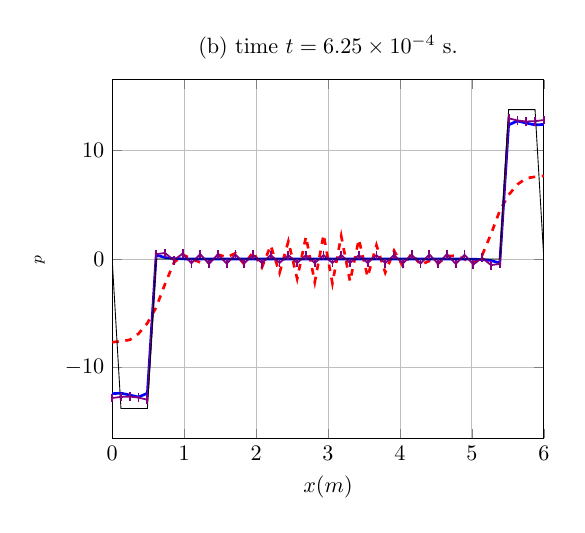
\begin{tikzpicture}[scale=0.8]
\begin{axis}[xlabel=$x (m)$,ylabel=$\eps^p$,ymajorgrids=true,xmajorgrids=true,legend pos=outer north east,title={(b) time $t = 6.25\times 10^{-4} $ s.},xmin=0.,xmax=6.]
\addplot[Red,very thick,mark=none,dashed] coordinates {(0.0,-7.656775715214294) (0.12244897959183673,-7.571339609307247) (0.24489795918367346,-7.438298117574187) (0.36734693877551017,-6.871029176921102) (0.4897959183673469,-5.903192627910385) (0.6122448979591837,-4.452057017543719) (0.7346938775510203,-2.3010481858807137) (0.8571428571428571,-0.3610443561643931) (0.9795918367346939,0.4188880742890505) (1.1020408163265305,0.01523876833598381) (1.2244897959183674,-0.3087249726610329) (1.346938775510204,-0.2682346195141458) (1.4693877551020407,0.41346894641452914) (1.5918367346938775,0.17204334381941044) (1.7142857142857142,0.5321881814826378) (1.836734693877551,-0.5074097815176064) (1.9591836734693877,0.6574508309639426) (2.0816326530612246,-0.7746969731901449) (2.204081632653061,1.2501366726613066) (2.326530612244898,-1.2807853076694733) (2.4489795918367347,1.631639383742251) (2.571428571428571,-1.8095691375383345) (2.693877551020408,2.0564749800644937) (2.816326530612245,-2.129190071354842) (2.9387755102040813,2.240060604992734) (3.061224489795918,-2.240060604992724) (3.183673469387755,2.1291900713548246) (3.306122448979592,-2.0564749800644746) (3.4285714285714284,1.809569137538315) (3.5510204081632653,-1.6316393837422516) (3.673469387755102,1.2807853076694653) (3.7959183673469385,-1.2501366726612742) (3.9183673469387754,0.7746969731901434) (4.040816326530612,-0.657450830963913) (4.163265306122449,0.5074097815175931) (4.285714285714286,-0.5321881814826224) (4.408163265306122,-0.17204334381940892) (4.530612244897959,-0.41346894641450627) (4.653061224489796,0.2682346195141527) (4.775510204081632,0.3087249726610414) (4.8979591836734695,-0.015238768335992692) (5.020408163265306,-0.4188880742890616) (5.142857142857142,0.3610443561643748) (5.26530612244898,2.3010481858807146) (5.387755102040816,4.452057017543711) (5.5102040816326525,5.90319262791038) (5.63265306122449,6.871029176921099) (5.755102040816326,7.4382981175741865) (5.877551020408163,7.571339609307248) (6.0,7.656775715214293) };
\addplot[Blue,very thick,mark=none,solid] coordinates {(0.0,-12.397952325377972) (0.12244897959183673,-12.346999574642966) (0.24489795918367346,-12.523092906128134) (0.36734693877551017,-12.71053547781855) (0.4897959183673469,-12.35049907311499) (0.6122448979591837,0.3722186738331613) (0.7346938775510203,0.1368090990556044) (0.8571428571428571,0.04446044382179651) (0.9795918367346939,0.012779812577704604) (1.1020408163265305,0.0032485856428356346) (1.2244897959183674,0.0007296815528062405) (1.346938775510204,0.00014459919089050038) (1.4693877551020407,2.5219563746036564e-05) (1.5918367346938775,3.857895635058131e-06) (1.7142857142857142,5.15199447901326e-07) (1.836734693877551,5.969388946802084e-08) (1.9591836734693877,5.952534698926585e-09) (2.0816326530612246,5.054662228331333e-10) (2.204081632653061,3.605726635043781e-11) (2.326530612244898,2.127654817367282e-12) (2.4489795918367347,1.1360160010621981e-13) (2.571428571428571,1.3411408617982763e-14) (2.693877551020408,1.66517088668301e-14) (2.816326530612245,5.526766510246074e-15) (2.9387755102040813,6.098792312826054e-15) (3.061224489795918,2.7682726724007426e-15) (3.183673469387755,7.175699018437728e-15) (3.306122448979592,-1.434813028923028e-14) (3.4285714285714284,-8.513769125527232e-15) (3.5510204081632653,-1.0095742773609699e-13) (3.673469387755102,-2.1199430888032018e-12) (3.7959183673469385,-3.6039619852103143e-11) (3.9183673469387754,-5.0545241703127e-10) (4.040816326530612,-5.9525221489037014e-09) (4.163265306122449,-5.969386814802888e-08) (4.285714285714286,-5.151994230605103e-07) (4.408163265306122,-3.8578956228878976e-06) (4.530612244897959,-2.5219563737562718e-05) (4.653061224489796,-0.00014459919087944834) (4.775510204081632,-0.0007296815527927886) (4.8979591836734695,-0.0032485856428289012) (5.020408163265306,-0.012779812577696097) (5.142857142857142,-0.04446044382178102) (5.26530612244898,-0.13680909905559333) (5.387755102040816,-0.3722186738331447) (5.5102040816326525,12.350499073115015) (5.63265306122449,12.71053547781857) (5.755102040816326,12.523092906128156) (5.877551020408163,12.346999574642979) (6.0,12.39795232537799) };
\addplot[Purple,thick,mark=|,solid] coordinates {(0.0,-12.795628373535159) (0.12244897959183673,-12.695543273778933) (0.24489795918367346,-12.666110940711564) (0.36734693877551017,-12.75241410003132) (0.4897959183673469,-12.960739789752774) (0.6122448979591837,0.44192323057668886) (0.7346938775510203,0.5605175207125453) (0.8571428571428571,-0.1118177278404644) (0.9795918367346939,0.49857571480888807) (1.1020408163265305,-0.3912177295445921) (1.2244897959183674,0.45869222504142426) (1.346938775510204,-0.4542184988816014) (1.4693877551020407,0.4392500135640788) (1.5918367346938775,-0.4268192827562814) (1.7142857142857142,0.4185270888397142) (1.836734693877551,-0.39693938041336063) (1.9591836734693877,0.398295251539175) (2.0816326530612246,-0.37211426798041747) (2.204081632653061,0.37593537352436907) (2.326530612244898,-0.3607380778681954) (2.4489795918367347,0.36132221537101705) (2.571428571428571,-0.3654682237983432) (2.693877551020408,0.35826901292698654) (2.816326530612245,-0.3691156051231741) (2.9387755102040813,0.36040411668068795) (3.061224489795918,-0.3604041166806867) (3.183673469387755,0.369115605123182) (3.306122448979592,-0.3582690129270081) (3.4285714285714284,0.36546822379836186) (3.5510204081632653,-0.3613222153709926) (3.673469387755102,0.3607380778681742) (3.7959183673469385,-0.37593537352436845) (3.9183673469387754,0.37211426798044456) (4.040816326530612,-0.3982952515391655) (4.163265306122449,0.3969393804133886) (4.285714285714286,-0.4185270888397233) (4.408163265306122,0.42681928275629366) (4.530612244897959,-0.43925001356404864) (4.653061224489796,0.45421849888160465) (4.775510204081632,-0.4586922250414254) (4.8979591836734695,0.3912177295446241) (5.020408163265306,-0.4985757148088702) (5.142857142857142,0.11181772784050628) (5.26530612244898,-0.560517520712548) (5.387755102040816,-0.4419232305766629) (5.5102040816326525,12.960739789752816) (5.63265306122449,12.75241410003134) (5.755102040816326,12.666110940711583) (5.877551020408163,12.695543273778958) (6.0,12.795628373535196) };
\addplot[black,thin,mark=none,solid] coordinates {(0.0,-0.0) (0.12244897959183673,-13.758687910475539) (0.24489795918367346,-13.758687910475539) (0.36734693877551017,-13.758687910475539) (0.4897959183673469,-13.758687910475539) (0.6122448979591837,-0.0) (0.7346938775510203,-0.0) (0.8571428571428571,-0.0) (0.9795918367346939,-0.0) (1.1020408163265305,-0.0) (1.2244897959183674,-0.0) (1.346938775510204,-0.0) (1.4693877551020407,-0.0) (1.5918367346938775,-0.0) (1.7142857142857142,-0.0) (1.836734693877551,-0.0) (1.9591836734693877,-0.0) (2.0816326530612246,-0.0) (2.204081632653061,-0.0) (2.326530612244898,-0.0) (2.4489795918367347,-0.0) (2.571428571428571,-0.0) (2.693877551020408,-0.0) (2.816326530612245,-0.0) (2.9387755102040813,-0.0) (3.061224489795918,-0.0) (3.183673469387755,-0.0) (3.306122448979592,-0.0) (3.4285714285714284,-0.0) (3.5510204081632653,-0.0) (3.673469387755102,-0.0) (3.7959183673469385,-0.0) (3.9183673469387754,-0.0) (4.040816326530612,-0.0) (4.163265306122449,-0.0) (4.285714285714286,-0.0) (4.408163265306122,-0.0) (4.530612244897959,-0.0) (4.653061224489796,-0.0) (4.775510204081632,-0.0) (4.8979591836734695,-0.0) (5.020408163265306,-0.0) (5.142857142857142,-0.0) (5.26530612244898,-0.0) (5.387755102040816,-0.0) (5.5102040816326525,13.758687910475539) (5.63265306122449,13.758687910475539) (5.755102040816326,13.758687910475539) (5.877551020408163,13.758687910475539) (6.0,0.0) };
%\legend{usl 1ppc,dgmpm 1ppc (ep solver),dgmpm 1ppc (ac solver),exact}
\end{axis}
\end{tikzpicture}
%%% Local Variables:
%%% mode: latex
%%% TeX-master: "../../mainManuscript"
%%% End:
}
%   {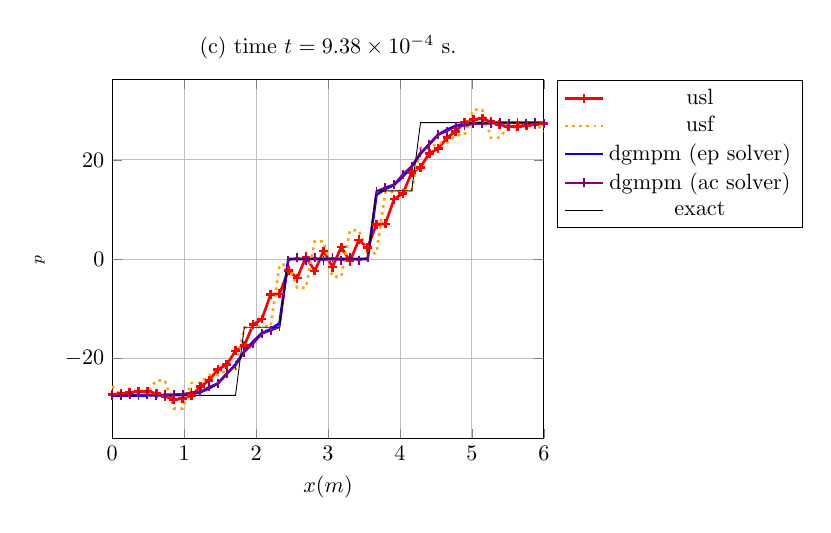
\begin{tikzpicture}[scale=0.8]
\begin{axis}[xlabel=$x (m)$,ylabel=$\eps^p$,ymajorgrids=true,xmajorgrids=true,legend pos=outer north east,title={(c) time $t = 9.38\times 10^{-4} $ s.},xmin=0.,xmax=6.]
\addplot[Red,very thick,mark=+,solid] coordinates {(0.0,-27.331872449853556) (0.12244897959183673,-27.174400085417467) (0.24489795918367346,-26.904779830121768) (0.36734693877551017,-26.69301343005911) (0.4897959183673469,-26.683543140751915) (0.6122448979591837,-27.106963962300345) (0.7346938775510203,-27.704030887608354) (0.8571428571428571,-28.33906014232905) (0.9795918367346939,-28.167172814076366) (1.1020408163265305,-27.53334986092529) (1.2244897959183674,-25.775044707062726) (1.346938775510204,-24.466615882102165) (1.4693877551020407,-22.247186500301964) (1.5918367346938775,-21.33079179039491) (1.7142857142857142,-18.523714044368063) (1.836734693877551,-17.44233776410034) (1.9591836734693877,-13.237799741628182) (2.0816326530612246,-12.0894356407598) (2.204081632653061,-7.096371776087362) (2.326530612244898,-7.032925295785245) (2.4489795918367347,-2.2620897664972315) (2.571428571428571,-3.858668388515009) (2.693877551020408,0.4300541105363164) (2.816326530612245,-2.410115988529146) (2.9387755102040813,1.6326922086221445) (3.061224489795918,-1.6326922086221325) (3.183673469387755,2.410115988529122) (3.306122448979592,-0.43005411053631265) (3.4285714285714284,3.858668388514974) (3.5510204081632653,2.2620897664972395) (3.673469387755102,7.032925295785231) (3.7959183673469385,7.096371776087392) (3.9183673469387754,12.089435640759786) (4.040816326530612,13.237799741628214) (4.163265306122449,17.442337764100337) (4.285714285714286,18.523714044368088) (4.408163265306122,21.330791790394894) (4.530612244897959,22.247186500301982) (4.653061224489796,24.466615882102147) (4.775510204081632,25.775044707062744) (4.8979591836734695,27.53334986092529) (5.020408163265306,28.167172814076363) (5.142857142857142,28.33906014232903) (5.26530612244898,27.70403088760834) (5.387755102040816,27.106963962300348) (5.5102040816326525,26.683543140751933) (5.63265306122449,26.693013430059132) (5.755102040816326,26.904779830121797) (5.877551020408163,27.17440008541749) (6.0,27.331872449853574) };
\addplot[Orange,very thick,mark=none,dotted] coordinates {(0.0,-25.658312786761723) (0.12244897959183673,-27.51413969235028) (0.24489795918367346,-27.514139692350327) (0.36734693877551017,-26.86847994686687) (0.4897959183673469,-26.868479946866948) (0.6122448979591837,-24.492978695040286) (0.7346938775510203,-24.49297869504042) (0.8571428571428571,-30.15019249346318) (0.9795918367346939,-30.15019249346324) (1.1020408163265305,-24.98956773450457) (1.2244897959183674,-24.98956773450463) (1.346938775510204,-23.40942037125753) (1.4693877551020407,-23.409420371257625) (1.5918367346938775,-22.418334622056513) (1.7142857142857142,-22.418334622056435) (1.836734693877551,-13.85468254978275) (1.9591836734693877,-13.854682549782833) (2.0816326530612246,-13.574506608280911) (2.204081632653061,-13.574506608280759) (2.326530612244898,-1.1520841431514552) (2.4489795918367347,-1.1520841431514355) (2.571428571428571,-5.798608057459956) (2.693877551020408,-5.7986080574598535) (2.816326530612245,3.5614225712693863) (2.9387755102040813,3.5614225712696768) (3.061224489795918,-3.5614225712695777) (3.183673469387755,-3.561422571269489) (3.306122448979592,5.798608057459823) (3.4285714285714284,5.798608057459984) (3.5510204081632653,1.1520841431513575) (3.673469387755102,1.152084143151603) (3.7959183673469385,13.574506608280872) (3.9183673469387754,13.574506608280805) (4.040816326530612,13.854682549782702) (4.163265306122449,13.854682549782932) (4.285714285714286,22.418334622056502) (4.408163265306122,22.418334622056456) (4.530612244897959,23.409420371257596) (4.653061224489796,23.40942037125754) (4.775510204081632,24.989567734504483) (4.8979591836734695,24.98956773450469) (5.020408163265306,30.150192493463102) (5.142857142857142,30.15019249346332) (5.26530612244898,24.49297869504033) (5.387755102040816,24.492978695040364) (5.5102040816326525,26.868479946866863) (5.63265306122449,26.86847994686695) (5.755102040816326,27.51413969235029) (5.877551020408163,27.51413969235035) (6.0,25.65831278676172) };
\addplot[Blue,very thick,mark=none,solid] coordinates {(0.0,-27.517363397075158) (0.12244897959183673,-27.51732379155038) (0.24489795918367346,-27.517228936294842) (0.36734693877551017,-27.516689788484122) (0.4897959183673469,-27.51556852970287) (0.6122448979591837,-27.51025382248486) (0.7346938775510203,-27.500198710367762) (0.8571428571428571,-27.46081288016468) (0.9795918367346939,-27.394149463815683) (1.1020408163265305,-27.182111927326957) (1.2244897959183674,-26.86831399158136) (1.346938775510204,-26.078149290066197) (1.4693877551020407,-25.088393528723113) (1.5918367346938775,-23.18951900040588) (1.7142857142857142,-21.27348955232938) (1.836734693877551,-18.64183859399964) (1.9591836734693877,-16.674856395188144) (2.0816326530612246,-14.952075198356093) (2.204081632653061,-14.149762008703409) (2.326530612244898,-12.97119731020455) (2.4489795918367347,1.4749921389468362e-14) (2.571428571428571,2.901956841536459e-14) (2.693877551020408,2.1854428799290698e-14) (2.816326530612245,2.1134926307627894e-14) (2.9387755102040813,2.170695211020788e-14) (3.061224489795918,2.3579152402243164e-14) (3.183673469387755,1.2378418950898343e-14) (3.306122448979592,1.1665469373072734e-14) (3.4285714285714284,7.094390671854583e-15) (3.5510204081632653,8.299690845575712e-15) (3.673469387755102,12.971197310204621) (3.7959183673469385,14.149762008703473) (3.9183673469387754,14.952075198356113) (4.040816326530612,16.674856395188158) (4.163265306122449,18.641838593999683) (4.285714285714286,21.273489552329384) (4.408163265306122,23.189519000405888) (4.530612244897959,25.088393528723138) (4.653061224489796,26.07814929006618) (4.775510204081632,26.868313991581342) (4.8979591836734695,27.182111927326957) (5.020408163265306,27.3941494638157) (5.142857142857142,27.46081288016466) (5.26530612244898,27.500198710367762) (5.387755102040816,27.51025382248485) (5.5102040816326525,27.515568529702865) (5.63265306122449,27.51668978848415) (5.755102040816326,27.517228936294806) (5.877551020408163,27.517323791550382) (6.0,27.517363397075165) };
\addplot[Purple,thick,mark=|,solid] coordinates {(0.0,-27.455491898583844) (0.12244897959183673,-27.52990791746212) (0.24489795918367346,-27.39669410111553) (0.36734693877551017,-27.56069772218648) (0.4897959183673469,-27.354208534961813) (0.6122448979591837,-27.484169218141297) (0.7346938775510203,-27.30529154707286) (0.8571428571428571,-27.260887430891447) (0.9795918367346939,-27.234362200737557) (1.1020408163265305,-26.87048565463221) (1.2244897959183674,-26.76603983934888) (1.346938775510204,-25.75807449243556) (1.4693877551020407,-25.06955937174821) (1.5918367346938775,-23.02673771458467) (1.7142857142857142,-21.509235536573875) (1.836734693877551,-18.773874989550777) (1.9591836734693877,-17.141311478227397) (2.0816326530612246,-15.098912535609557) (2.204081632653061,-14.451161421148855) (2.326530612244898,-13.715612700621918) (2.4489795918367347,-0.23693029878140853) (2.571428571428571,0.24220658661539068) (2.693877551020408,-0.22882318056987147) (2.816326530612245,0.2316928153217551) (2.9387755102040813,-0.22713962166300733) (3.061224489795918,0.22713962166305024) (3.183673469387755,-0.2316928153217785) (3.306122448979592,0.22882318056992768) (3.4285714285714284,-0.24220658661539307) (3.5510204081632653,0.23693029878141705) (3.673469387755102,13.71561270062201) (3.7959183673469385,14.451161421148875) (3.9183673469387754,15.098912535609603) (4.040816326530612,17.141311478227408) (4.163265306122449,18.77387498955077) (4.285714285714286,21.509235536573904) (4.408163265306122,23.026737714584694) (4.530612244897959,25.06955937174818) (4.653061224489796,25.758074492435522) (4.775510204081632,26.766039839348913) (4.8979591836734695,26.870485654632194) (5.020408163265306,27.23436220073757) (5.142857142857142,27.260887430891422) (5.26530612244898,27.305291547072898) (5.387755102040816,27.484169218141297) (5.5102040816326525,27.354208534961796) (5.63265306122449,27.560697722186475) (5.755102040816326,27.39669410111557) (5.877551020408163,27.529907917462097) (6.0,27.455491898583855) };
\addplot[black,thin,mark=none,solid] coordinates {(0.0,-27.517375820951077) (0.12244897959183673,-27.517375820951077) (0.24489795918367346,-27.517375820951077) (0.36734693877551017,-27.517375820951077) (0.4897959183673469,-27.517375820951077) (0.6122448979591837,-27.517375820951077) (0.7346938775510203,-27.517375820951077) (0.8571428571428571,-27.517375820951077) (0.9795918367346939,-27.517375820951077) (1.1020408163265305,-27.517375820951077) (1.2244897959183674,-27.517375820951077) (1.346938775510204,-27.517375820951077) (1.4693877551020407,-27.517375820951077) (1.5918367346938775,-27.517375820951077) (1.7142857142857142,-27.517375820951077) (1.836734693877551,-13.758687910475539) (1.9591836734693877,-13.758687910475539) (2.0816326530612246,-13.758687910475539) (2.204081632653061,-13.758687910475539) (2.326530612244898,-13.758687910475539) (2.4489795918367347,-0.0) (2.571428571428571,-0.0) (2.693877551020408,-0.0) (2.816326530612245,-0.0) (2.9387755102040813,-0.0) (3.061224489795918,-0.0) (3.183673469387755,-0.0) (3.306122448979592,-0.0) (3.4285714285714284,-0.0) (3.5510204081632653,-0.0) (3.673469387755102,13.758687910475539) (3.7959183673469385,13.758687910475539) (3.9183673469387754,13.758687910475539) (4.040816326530612,13.758687910475539) (4.163265306122449,13.758687910475539) (4.285714285714286,27.517375820951077) (4.408163265306122,27.517375820951077) (4.530612244897959,27.517375820951077) (4.653061224489796,27.517375820951077) (4.775510204081632,27.517375820951077) (4.8979591836734695,27.517375820951077) (5.020408163265306,27.517375820951077) (5.142857142857142,27.517375820951077) (5.26530612244898,27.517375820951077) (5.387755102040816,27.517375820951077) (5.5102040816326525,27.517375820951077) (5.63265306122449,27.517375820951077) (5.755102040816326,27.517375820951077) (5.877551020408163,27.517375820951077) (6.0,27.517375820951077) };
\legend{usl,usf,dgmpm (ep solver),dgmpm (ac solver),exact}
\end{axis}
\end{tikzpicture}
%%% Local Variables:
%%% mode: latex
%%% TeX-master: "../../mainManuscript"
%%% End:
}
%   \caption{elastic-plastic RP velo}
%   \label{fig:velo_elastoplastic_RP}
% \end{figure}


Comparison with mpm for 1ppc and 2ppcs with RK2 (requires additional bc treatment and constitutive). Only ep solver
%%%%%%%%%%%%%%%%%%%%%%%%%%%%%%%%%%%%%%%%%%%%%%%%%%%%%%%%%%%%%%%%%%%%%
% \begin{figure}[h!]
%   \centering
%   {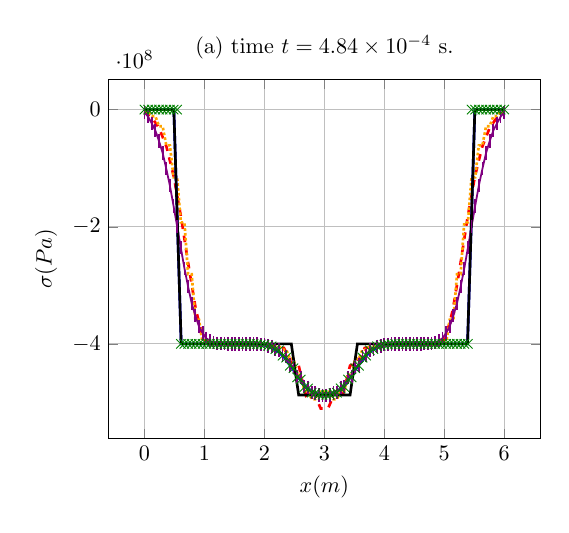
\begin{tikzpicture}[scale=0.8]
\begin{axis}[xlabel=$x (m)$,ylabel=$\sigma (Pa)$,ymajorgrids=true,xmajorgrids=true,legend pos=outer north east,title={(a) time $t = 4.84\times 10^{-4} $ s.}]
\addplot[Red,very thick,mark=none,dashed,mark size=3pt] coordinates {(0.0,-3669561.908091424) (0.12244897959183673,-13594450.379485756) (0.24489795918367346,-31624435.10565728) (0.36734693877551017,-63707048.32128755) (0.4897959183673469,-114660806.5675256) (0.6122448979591837,-184794660.6509606) (0.7346938775510203,-266179173.63903272) (0.8571428571428571,-341775310.1478163) (0.9795918367346939,-390693099.4776282) (1.1020408163265305,-400379159.02115166) (1.2244897959183674,-400770866.2752631) (1.346938775510204,-400849758.67078286) (1.4693877551020407,-400903087.2437715) (1.5918367346938775,-400974206.0457186) (1.7142857142857142,-401177729.4632526) (1.836734693877551,-401187799.71208847) (1.9591836734693877,-401722959.3911894) (2.0816326530612246,-401625095.9277148) (2.204081632653061,-405721718.460188) (2.326530612244898,-406980928.2270958) (2.4489795918367347,-432556847.70391244) (2.571428571428571,-437038541.50331527) (2.693877551020408,-488555362.3021708) (2.816326530612245,-481341619.82050365) (2.9387755102040813,-510307309.7388937) (3.061224489795918,-510307309.7388923) (3.183673469387755,-481341619.8205054) (3.306122448979592,-488555362.3021694) (3.4285714285714284,-437038541.50331557) (3.5510204081632653,-432556847.70391184) (3.673469387755102,-406980928.2270957) (3.7959183673469385,-405721718.4601879) (3.9183673469387754,-401625095.9277147) (4.040816326530612,-401722959.3911895) (4.163265306122449,-401187799.71208847) (4.285714285714286,-401177729.4632526) (4.408163265306122,-400974206.0457186) (4.530612244897959,-400903087.2437715) (4.653061224489796,-400849758.670783) (4.775510204081632,-400770866.2752632) (4.8979591836734695,-400379159.02115154) (5.020408163265306,-390693099.47762805) (5.142857142857142,-341775310.1478161) (5.26530612244898,-266179173.63903314) (5.387755102040816,-184794660.65096068) (5.5102040816326525,-114660806.56752594) (5.63265306122449,-63707048.32128816) (5.755102040816326,-31624435.10565742) (5.877551020408163,-13594450.3794861) (6.0,-3669561.9080915614) };
\addplot[Orange,very thick,mark=none,densely dotted,mark size=3pt] coordinates {(0.0,-2914267.3201301154) (0.06060606060606061,-2914267.3201301154) (0.12121212121212122,-11378318.451142035) (0.18181818181818182,-11378318.451142035) (0.24242424242424243,-28406466.993262846) (0.30303030303030304,-28406466.993262846) (0.36363636363636365,-61055835.593559496) (0.42424242424242425,-61055835.593559496) (0.48484848484848486,-115583582.76704544) (0.5454545454545454,-115583582.76704544) (0.6060606060606061,-192564241.19110337) (0.6666666666666667,-192564241.19110337) (0.7272727272727273,-281227079.2224079) (0.7878787878787878,-281227079.2224079) (0.8484848484848485,-358622783.83691025) (0.9090909090909092,-358622783.83691025) (0.9696969696969697,-399584151.64208454) (1.0303030303030303,-399584151.64208454) (1.0909090909090908,-400518950.3403047) (1.1515151515151516,-400518950.3403047) (1.2121212121212122,-400764480.1267914) (1.2727272727272727,-400764480.1267914) (1.3333333333333335,-400835508.12332404) (1.393939393939394,-400835508.12332404) (1.4545454545454546,-400891006.2882111) (1.5151515151515151,-400891006.2882111) (1.5757575757575757,-400939762.1508219) (1.6363636363636365,-400939762.1508219) (1.696969696969697,-401049302.5008664) (1.7575757575757576,-401049302.5008664) (1.8181818181818183,-401273466.6129426) (1.878787878787879,-401273466.6129426) (1.9393939393939394,-401521516.00275475) (2.0,-401521516.00275475) (2.0606060606060606,-402092208.5638283) (2.121212121212121,-402092208.5638283) (2.1818181818181817,-404027519.3843328) (2.2424242424242427,-404027519.3843328) (2.303030303030303,-409750544.23386204) (2.3636363636363638,-409750544.23386204) (2.4242424242424243,-425145499.736588) (2.484848484848485,-425145499.736588) (2.5454545454545454,-452445709.1416535) (2.606060606060606,-452445709.1416535) (2.666666666666667,-479926155.3868412) (2.7272727272727275,-479926155.3868412) (2.787878787878788,-494460484.088121) (2.8484848484848486,-494460484.088121) (2.909090909090909,-481596066.8615678) (2.9696969696969697,-481596066.8615678) (3.0303030303030303,-481596066.8615678) (3.090909090909091,-481596066.8615678) (3.1515151515151514,-494460484.088121) (3.2121212121212124,-494460484.088121) (3.272727272727273,-479926155.3868412) (3.3333333333333335,-479926155.3868412) (3.393939393939394,-452445709.1416535) (3.4545454545454546,-452445709.1416535) (3.515151515151515,-425145499.736588) (3.5757575757575757,-425145499.736588) (3.6363636363636367,-409750544.23386204) (3.6969696969696972,-409750544.23386204) (3.757575757575758,-404027519.3843328) (3.8181818181818183,-404027519.3843328) (3.878787878787879,-402092208.5638283) (3.9393939393939394,-402092208.5638283) (4.0,-401521516.0027547) (4.0606060606060606,-401521516.0027547) (4.121212121212121,-401273466.6129426) (4.181818181818182,-401273466.6129426) (4.242424242424242,-401049302.5008665) (4.303030303030303,-401049302.5008665) (4.363636363636363,-400939762.15082186) (4.424242424242425,-400939762.15082186) (4.484848484848485,-400891006.2882111) (4.545454545454546,-400891006.2882111) (4.606060606060606,-400835508.12332404) (4.666666666666667,-400835508.12332404) (4.7272727272727275,-400764480.1267914) (4.787878787878788,-400764480.1267914) (4.848484848484849,-400518950.3403046) (4.909090909090909,-400518950.3403046) (4.96969696969697,-399584151.6420844) (5.03030303030303,-399584151.6420844) (5.090909090909091,-358622783.8369101) (5.151515151515151,-358622783.8369101) (5.212121212121212,-281227079.22240764) (5.2727272727272725,-281227079.22240764) (5.333333333333334,-192564241.19110358) (5.3939393939393945,-192564241.19110358) (5.454545454545455,-115583582.76704524) (5.515151515151516,-115583582.76704524) (5.575757575757576,-61055835.59355964) (5.636363636363637,-61055835.59355964) (5.696969696969697,-28406466.99326251) (5.757575757575758,-28406466.99326251) (5.818181818181818,-11378318.451142171) (5.878787878787879,-11378318.451142171) (5.9393939393939394,-2914267.3201301834) (6.0,-2914267.3201301834) };
\addplot[Blue,very thick,mark=none,solid,mark size=3pt] coordinates {(0.0,-1.4032094709741823e-07) (0.12244897959183673,1.4032094709741797e-07) (0.24489795918367346,-5.501313561848306e-23) (0.36734693877551017,-1.4032094709741882e-07) (0.4897959183673469,-4.2096284129225576e-07) (0.6122448979591837,-400000000.0000052) (0.7346938775510203,-400000000.0003803) (0.8571428571428571,-400000000.0131417) (0.9795918367346939,-400000000.2874559) (1.1020408163265305,-400000004.46415013) (1.2244897959183674,-400000052.34678423) (1.346938775510204,-400000481.2046858) (1.4693877551020407,-400003554.03647596) (1.5918367346938775,-400021443.0967657) (1.7142857142857142,-400106894.9802318) (1.836734693877551,-400443646.6051052) (1.9591836734693877,-401540408.59283984) (2.0816326530612246,-404487333.2231472) (2.204081632653061,-410984305.87262785) (2.326530612244898,-422622254.02503896) (2.4489795918367347,-439299786.1010327) (2.571428571428571,-457971198.93456453) (2.693877551020408,-473710434.18348145) (2.816326530612245,-483108267.7934754) (2.9387755102040813,-486652315.1909913) (3.061224489795918,-486652315.1909913) (3.183673469387755,-483108267.7934754) (3.306122448979592,-473710434.18348145) (3.4285714285714284,-457971198.93456453) (3.5510204081632653,-439299786.1010328) (3.673469387755102,-422622254.025039) (3.7959183673469385,-410984305.8726279) (3.9183673469387754,-404487333.2231472) (4.040816326530612,-401540408.59283984) (4.163265306122449,-400443646.6051051) (4.285714285714286,-400106894.98023176) (4.408163265306122,-400021443.0967656) (4.530612244897959,-400003554.0364758) (4.653061224489796,-400000481.20468575) (4.775510204081632,-400000052.3467841) (4.8979591836734695,-400000004.46415013) (5.020408163265306,-400000000.2874559) (5.142857142857142,-400000000.01314175) (5.26530612244898,-400000000.0003803) (5.387755102040816,-400000000.0000052) (5.5102040816326525,1.403209470974181e-07) (5.63265306122449,-4.209628412922546e-07) (5.755102040816326,-7.335084749131074e-23) (5.877551020408163,-7.335084749131074e-23) (6.0,1.4032094709741816e-07) };
\addplot[Purple,thick,mark=|,solid,mark size=3pt] coordinates {(0.0,-4432924.706841537) (0.06060606060606061,-12207367.937325412) (0.12121212121212122,-23531843.32279323) (0.18181818181818182,-35734156.38126936) (0.24242424242424243,-53819967.0341102) (0.30303030303030304,-73960503.34391399) (0.36363636363636365,-100971777.07395627) (0.42424242424242425,-130109924.83030084) (0.48484848484848486,-164461120.69762146) (0.5454545454545454,-199783681.59143203) (0.6060606060606061,-235957589.20194656) (0.6666666666666667,-271228096.10690445) (0.7272727272727273,-302213993.4219046) (0.7878787878787878,-330771054.2743039) (0.8484848484848485,-351899554.770462) (0.9090909090909092,-370258280.79493797) (0.9696969696969697,-381361519.41978526) (1.0303030303030303,-390443246.24646133) (1.0909090909090908,-394697061.64063984) (1.1515151515151516,-397978403.46801) (1.2121212121212122,-399033797.91006035) (1.2727272727272727,-399815009.1781527) (1.3333333333333335,-399928549.7385389) (1.393939393939394,-400001024.16277933) (1.4545454545454546,-400002181.8139095) (1.5151515151515151,-400003409.2713153) (1.5757575757575757,-400013260.9517136) (1.6363636363636365,-400019327.12601054) (1.696969696969697,-400071982.9779926) (1.7575757575757576,-400098745.1685716) (1.8181818181818183,-400318321.7394188) (1.878787878787879,-400414890.0391485) (1.9393939393939394,-401165297.85083073) (2.0,-401450756.0252169) (2.0606060606060606,-403565545.76565593) (2.121212121212121,-404257062.9865757) (2.1818181818181817,-409162020.12612975) (2.2424242424242427,-410524033.8850246) (2.303030303030303,-419802201.6406596) (2.3636363636363638,-421949146.8716409) (2.4242424242424243,-436028496.5842672) (2.484848484848485,-438667957.45895886) (2.5454545454545454,-455363332.4481878) (2.606060606060606,-457791067.839726) (2.666666666666667,-472627847.3837442) (2.7272727272727275,-474182129.162814) (2.787878787878788,-483383494.6652765) (2.8484848484848486,-483980615.0668598) (2.909090909090909,-487493210.5310644) (2.9696969696969697,-487590657.9314887) (3.0303030303030303,-487590657.9314887) (3.090909090909091,-487493210.5310644) (3.1515151515151514,-483980615.0668598) (3.2121212121212124,-483383494.6652765) (3.272727272727273,-474182129.162814) (3.3333333333333335,-472627847.38374436) (3.393939393939394,-457791067.839726) (3.4545454545454546,-455363332.4481878) (3.515151515151515,-438667957.458959) (3.5757575757575757,-436028496.5842673) (3.6363636363636367,-421949146.871641) (3.6969696969696972,-419802201.6406597) (3.757575757575758,-410524033.8850248) (3.8181818181818183,-409162020.1261299) (3.878787878787879,-404257062.98657584) (3.9393939393939394,-403565545.765656) (4.0,-401450756.0252169) (4.0606060606060606,-401165297.85083085) (4.121212121212121,-400414890.0391486) (4.181818181818182,-400318321.7394188) (4.242424242424242,-400098745.1685716) (4.303030303030303,-400071982.9779927) (4.363636363636363,-400019327.12601066) (4.424242424242425,-400013260.95171374) (4.484848484848485,-400003409.2713153) (4.545454545454546,-400002181.8139095) (4.606060606060606,-400001024.16277933) (4.666666666666667,-399928549.7385392) (4.7272727272727275,-399815009.17815316) (4.787878787878788,-399033797.9100607) (4.848484848484849,-397978403.46801054) (4.909090909090909,-394697061.6406404) (4.96969696969697,-390443246.24646163) (5.03030303030303,-381361519.4197858) (5.090909090909091,-370258280.7949385) (5.151515151515151,-351899554.7704626) (5.212121212121212,-330771054.27430445) (5.2727272727272725,-302213993.42190534) (5.333333333333334,-271228096.1069048) (5.3939393939393945,-235957589.201947) (5.454545454545455,-199783681.5914322) (5.515151515151516,-164461120.6976217) (5.575757575757576,-130109924.83030085) (5.636363636363637,-100971777.07395627) (5.696969696969697,-73960503.34391414) (5.757575757575758,-53819967.034110345) (5.818181818181818,-35734156.38126946) (5.878787878787879,-23531843.322793126) (5.9393939393939394,-12207367.937325357) (6.0,-4432924.706841591) };
\addplot[Green,thin,mark=x,only marks,mark size=3pt] coordinates {(0.0,1.2652173515404603e-06) (0.06060606060606061,9.799178020182319e-07) (0.12121212121212122,-4.084567774230407e-07) (0.18181818181818182,-4.3346890516146844e-07) (0.24242424242424243,4.563473356624432e-07) (0.30303030303030304,3.855783469220664e-07) (0.36363636363636365,-5.846850939002003e-07) (0.42424242424242425,-8.185243770739822e-07) (0.48484848484848486,5.883985548618523e-07) (0.5454545454545454,8.148109161123314e-07) (0.6060606060606061,-400000000.0000001) (0.6666666666666667,-400000000.0000003) (0.7272727272727273,-400000000.00001395) (0.7878787878787878,-400000000.0000309) (0.8484848484848485,-400000000.0007001) (0.9090909090909092,-400000000.0014903) (0.9696969696969697,-400000000.0219135) (1.0303030303030303,-400000000.0446493) (1.0909090909090908,-400000000.4778095) (1.1515151515151516,-400000000.93062043) (1.2121212121212122,-400000007.7115201) (1.2727272727272727,-400000014.3371707) (1.3333333333333335,-400000095.54857785) (1.393939393939394,-400000169.3314061) (1.4545454545454546,-400000930.466908) (1.5151515151515151,-400001569.6122349) (1.5757575757575757,-400007232.7377954) (1.6363636363636365,-400011597.9099656) (1.696969696969697,-400045337.5232003) (1.7575757575757576,-400069019.1005317) (1.8181818181818183,-400230656.1994125) (1.878787878787879,-400332993.2150553) (1.9393939393939394,-400955956.96957076) (2.0,-401307731.2616477) (2.0606060606060606,-403233382.7711176) (2.121212121212121,-404189912.7567165) (2.1818181818181817,-408931765.9664936) (2.2424242424242427,-410968365.8644036) (2.303030303030303,-420167583.50623786) (2.3636363636363638,-423508767.0960166) (2.4242424242424243,-437335267.865692) (2.484848484848485,-441457068.1017972) (2.5454545454545454,-457161702.9599444) (2.606060606060606,-460844115.7211842) (2.666666666666667,-473822399.01136905) (2.7272727272727275,-476062326.4885395) (2.787878787878788,-483396938.4157252) (2.8484848484848486,-484223655.8917301) (2.909090909090909,-486749500.07510275) (2.9696969696969697,-486888696.01046515) (3.0303030303030303,-486888696.01046515) (3.090909090909091,-486749500.07510275) (3.1515151515151514,-484223655.8917301) (3.2121212121212124,-483396938.4157252) (3.272727272727273,-476062326.4885395) (3.3333333333333335,-473822399.0113689) (3.393939393939394,-460844115.721184) (3.4545454545454546,-457161702.9599444) (3.515151515151515,-441457068.1017974) (3.5757575757575757,-437335267.865692) (3.6363636363636367,-423508767.0960167) (3.6969696969696972,-420167583.506238) (3.757575757575758,-410968365.8644036) (3.8181818181818183,-408931765.9664936) (3.878787878787879,-404189912.7567166) (3.9393939393939394,-403233382.7711176) (4.0,-401307731.2616477) (4.0606060606060606,-400955956.9695708) (4.121212121212121,-400332993.2150553) (4.181818181818182,-400230656.1994125) (4.242424242424242,-400069019.1005317) (4.303030303030303,-400045337.5232003) (4.363636363636363,-400011597.9099656) (4.424242424242425,-400007232.7377954) (4.484848484848485,-400001569.6122349) (4.545454545454546,-400000930.466908) (4.606060606060606,-400000169.3314062) (4.666666666666667,-400000095.5485779) (4.7272727272727275,-400000014.3371707) (4.787878787878788,-400000007.7115201) (4.848484848484849,-400000000.93062043) (4.909090909090909,-400000000.4778095) (4.96969696969697,-400000000.04464936) (5.03030303030303,-400000000.02191347) (5.090909090909091,-400000000.0014904) (5.151515151515151,-400000000.00070024) (5.212121212121212,-400000000.0000309) (5.2727272727272725,-400000000.0000138) (5.333333333333334,-400000000.00000036) (5.3939393939393945,-400000000.0000002) (5.454545454545455,5.066066144912661e-07) (5.515151515151516,6.159609622880803e-07) (5.575757575757576,-1.4374680478850218e-07) (5.636363636363637,-4.1753698360117076e-07) (5.696969696969697,-4.929735310217885e-07) (5.757575757575758,-6.295940457575577e-07) (5.818181818181818,1.5312531108404206e-06) (5.878787878787879,1.5558077253027814e-06) (5.9393939393939394,-3.6714372754933455e-07) (6.0,-1.9414006084033805e-07) };
\addplot[black,very thick,mark=pentagone*,solid,mark size=3pt] coordinates {(0.0,-0.0) (0.12244897959183673,-0.0) (0.24489795918367346,-0.0) (0.36734693877551017,-0.0) (0.4897959183673469,-0.0) (0.6122448979591837,-400000000.0) (0.7346938775510203,-400000000.0) (0.8571428571428571,-400000000.0) (0.9795918367346939,-400000000.0) (1.1020408163265305,-400000000.0) (1.2244897959183674,-400000000.0) (1.346938775510204,-400000000.0) (1.4693877551020407,-400000000.0) (1.5918367346938775,-400000000.0) (1.7142857142857142,-400000000.0) (1.836734693877551,-400000000.0) (1.9591836734693877,-400000000.0) (2.0816326530612246,-400000000.0) (2.204081632653061,-400000000.0) (2.326530612244898,-400000000.0) (2.4489795918367347,-400000000.0) (2.571428571428571,-487287156.09439695) (2.693877551020408,-487287156.09439695) (2.816326530612245,-487287156.09439695) (2.9387755102040813,-487287156.09439695) (3.061224489795918,-487287156.09439695) (3.183673469387755,-487287156.09439695) (3.306122448979592,-487287156.09439695) (3.4285714285714284,-487287156.09439695) (3.5510204081632653,-400000000.0) (3.673469387755102,-400000000.0) (3.7959183673469385,-400000000.0) (3.9183673469387754,-400000000.0) (4.040816326530612,-400000000.0) (4.163265306122449,-400000000.0) (4.285714285714286,-400000000.0) (4.408163265306122,-400000000.0) (4.530612244897959,-400000000.0) (4.653061224489796,-400000000.0) (4.775510204081632,-400000000.0) (4.8979591836734695,-400000000.0) (5.020408163265306,-400000000.0) (5.142857142857142,-400000000.0) (5.26530612244898,-400000000.0) (5.387755102040816,-400000000.0) (5.5102040816326525,-0.0) (5.63265306122449,-0.0) (5.755102040816326,-0.0) (5.877551020408163,-0.0) (6.0,-0.0) };
%\legend{usl 1ppc,usl 2ppc,dgmpm 1ppc,dgmpm 2ppc,dgmpm 2ppc (RK2),exact}
\end{axis}
\end{tikzpicture}
%%% Local Variables:
%%% mode: latex
%%% TeX-master: "../../mainManuscript"
%%% End:
}
%   {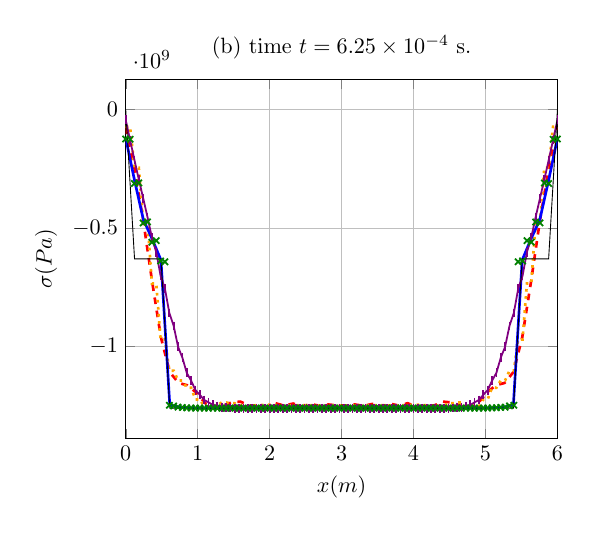
\begin{tikzpicture}[scale=0.8]
\begin{axis}[xlabel=$x (m)$,ylabel=$\sigma (Pa)$,ymajorgrids=true,xmajorgrids=true,legend pos=outer north east,title={(b) time $t = 6.25\times 10^{-4} $ s.},xmin=0.,xmax=6.]
\addplot[Red,very thick,mark=none,dashed] coordinates {(0.0,-74686690.65430246) (0.12244897959183673,-248860978.1693335) (0.24489795918367346,-471505677.3136862) (0.36734693877551017,-727347550.4714894) (0.4897959183673469,-963308331.6520433) (0.6122448979591837,-1108824904.6085515) (0.7346938775510203,-1154837713.915547) (0.8571428571428571,-1164658358.6882505) (0.9795918367346939,-1195327833.6731591) (1.1020408163265305,-1239722495.17177) (1.2244897959183674,-1262625036.5763078) (1.346938775510204,-1250850727.3360605) (1.4693877551020407,-1237335621.1098552) (1.5918367346938775,-1233570784.670482) (1.7142857142857142,-1250022356.590519) (1.836734693877551,-1250064510.2383804) (1.9591836734693877,-1255304260.9119728) (2.0816326530612246,-1240464014.9742188) (2.204081632653061,-1250749408.0219655) (2.326530612244898,-1241771881.0316234) (2.4489795918367347,-1254655253.5739675) (2.571428571428571,-1243386642.1602688) (2.693877551020408,-1251564997.8232079) (2.816326530612245,-1245650942.428049) (2.9387755102040813,-1249901934.3884947) (3.061224489795918,-1249901934.3884926) (3.183673469387755,-1245650942.4280505) (3.306122448979592,-1251564997.8232062) (3.4285714285714284,-1243386642.160271) (3.5510204081632653,-1254655253.5739667) (3.673469387755102,-1241771881.0316243) (3.7959183673469385,-1250749408.0219643) (3.9183673469387754,-1240464014.9742193) (4.040816326530612,-1255304260.911973) (4.163265306122449,-1250064510.238382) (4.285714285714286,-1250022356.59052) (4.408163265306122,-1233570784.670483) (4.530612244897959,-1237335621.1098552) (4.653061224489796,-1250850727.3360612) (4.775510204081632,-1262625036.5763083) (4.8979591836734695,-1239722495.1717708) (5.020408163265306,-1195327833.6731594) (5.142857142857142,-1164658358.688251) (5.26530612244898,-1154837713.915547) (5.387755102040816,-1108824904.6085508) (5.5102040816326525,-963308331.652042) (5.63265306122449,-727347550.4714878) (5.755102040816326,-471505677.3136848) (5.877551020408163,-248860978.16933236) (6.0,-74686690.65430167) };
\addplot[Orange,very thick,mark=none,dotted] coordinates {(0.0,-72186593.07108305) (0.06060606060606061,-72186593.07108305) (0.12121212121212122,-245686493.40496877) (0.18181818181818182,-245686493.40496877) (0.24242424242424243,-474670673.0513873) (0.30303030303030304,-474670673.0513873) (0.36363636363636365,-734906817.2671752) (0.42424242424242425,-734906817.2671752) (0.48484848484848486,-970962001.9023491) (0.5454545454545454,-970962001.9023491) (0.6060606060606061,-1103271474.8574238) (0.6666666666666667,-1103271474.8574238) (0.7272727272727273,-1144170322.1258416) (0.7878787878787878,-1144170322.1258416) (0.8484848484848485,-1175098111.1407657) (0.9090909090909092,-1175098111.1407657) (0.9696969696969697,-1224410658.5301867) (1.0303030303030303,-1224410658.5301867) (1.0909090909090908,-1254385387.017002) (1.1515151515151516,-1254385387.017002) (1.2121212121212122,-1249105579.9476206) (1.2727272727272727,-1249105579.9476206) (1.3333333333333335,-1237157219.1940255) (1.393939393939394,-1237157219.1940255) (1.4545454545454546,-1240480450.514414) (1.5151515151515151,-1240480450.514414) (1.5757575757575757,-1250188640.1270242) (1.6363636363636365,-1250188640.1270242) (1.696969696969697,-1252250954.763) (1.7575757575757576,-1252250954.763) (1.8181818181818183,-1248402726.9188023) (1.878787878787879,-1248402726.9188023) (1.9393939393939394,-1246829218.0208151) (2.0,-1246829218.0208151) (2.0606060606060606,-1248579916.6035461) (2.121212121212121,-1248579916.6035461) (2.1818181818181817,-1249829973.3539176) (2.2424242424242427,-1249829973.3539176) (2.303030303030303,-1249407075.968172) (2.3636363636363638,-1249407075.968172) (2.4242424242424243,-1248930440.9460857) (2.484848484848485,-1248930440.9460857) (2.5454545454545454,-1249182413.9939532) (2.606060606060606,-1249182413.9939532) (2.666666666666667,-1249584324.22758) (2.7272727272727275,-1249584324.22758) (2.787878787878788,-1249734146.6328998) (2.8484848484848486,-1249734146.6328998) (2.909090909090909,-1249747490.5668778) (2.9696969696969697,-1249747490.5668778) (3.0303030303030303,-1249747490.5668783) (3.090909090909091,-1249747490.5668783) (3.1515151515151514,-1249734146.6329007) (3.2121212121212124,-1249734146.6329007) (3.272727272727273,-1249584324.2275805) (3.3333333333333335,-1249584324.2275805) (3.393939393939394,-1249182413.993953) (3.4545454545454546,-1249182413.993953) (3.515151515151515,-1248930440.946085) (3.5757575757575757,-1248930440.946085) (3.6363636363636367,-1249407075.9681716) (3.6969696969696972,-1249407075.9681716) (3.757575757575758,-1249829973.3539178) (3.8181818181818183,-1249829973.3539178) (3.878787878787879,-1248579916.6035466) (3.9393939393939394,-1248579916.6035466) (4.0,-1246829218.0208151) (4.0606060606060606,-1246829218.0208151) (4.121212121212121,-1248402726.9188023) (4.181818181818182,-1248402726.9188023) (4.242424242424242,-1252250954.7630002) (4.303030303030303,-1252250954.7630002) (4.363636363636363,-1250188640.1270244) (4.424242424242425,-1250188640.1270244) (4.484848484848485,-1240480450.5144138) (4.545454545454546,-1240480450.5144138) (4.606060606060606,-1237157219.194025) (4.666666666666667,-1237157219.194025) (4.7272727272727275,-1249105579.9476204) (4.787878787878788,-1249105579.9476204) (4.848484848484849,-1254385387.0170026) (4.909090909090909,-1254385387.0170026) (4.96969696969697,-1224410658.5301871) (5.03030303030303,-1224410658.5301871) (5.090909090909091,-1175098111.140766) (5.151515151515151,-1175098111.140766) (5.212121212121212,-1144170322.125842) (5.2727272727272725,-1144170322.125842) (5.333333333333334,-1103271474.8574243) (5.3939393939393945,-1103271474.8574243) (5.454545454545455,-970962001.902349) (5.515151515151516,-970962001.902349) (5.575757575757576,-734906817.2671752) (5.636363636363637,-734906817.2671752) (5.696969696969697,-474670673.05138755) (5.757575757575758,-474670673.05138755) (5.818181818181818,-245686493.40496898) (5.878787878787879,-245686493.40496898) (5.9393939393939394,-72186593.0710832) (6.0,-72186593.0710832) };
\addplot[Blue,very thick,mark=none,solid] coordinates {(0.0,-120597397.19248778) (0.12244897959183673,-298539345.15508544) (0.24489795918367346,-464504460.170754) (0.36734693877551017,-546627376.3559334) (0.4897959183673469,-635546108.2543886) (0.6122448979591837,-1247334335.3333962) (0.7346938775510203,-1255980074.5990539) (0.8571428571428571,-1259371705.5275755) (0.9795918367346939,-1260535220.1287405) (1.1020408163265305,-1260885267.5005968) (1.2244897959183674,-1260977777.705495) (1.346938775510204,-1260999265.6570995) (1.4693877551020407,-1261003650.0375175) (1.5918367346938775,-1261004434.5740557) (1.7142857142857142,-1261004557.3391547) (1.836734693877551,-1261004574.0682204) (1.9591836734693877,-1261004576.0419452) (2.0816326530612246,-1261004576.241996) (2.204081632653061,-1261004576.2592359) (2.326530612244898,-1261004576.260481) (2.4489795918367347,-1261004576.260556) (2.571428571428571,-1261004576.2605588) (2.693877551020408,-1261004576.260559) (2.816326530612245,-1261004576.2605588) (2.9387755102040813,-1261004576.260559) (3.061224489795918,-1261004576.2605584) (3.183673469387755,-1261004576.2605586) (3.306122448979592,-1261004576.2605588) (3.4285714285714284,-1261004576.2605581) (3.5510204081632653,-1261004576.2605555) (3.673469387755102,-1261004576.260481) (3.7959183673469385,-1261004576.2592354) (3.9183673469387754,-1261004576.2419953) (4.040816326530612,-1261004576.0419443) (4.163265306122449,-1261004574.06822) (4.285714285714286,-1261004557.3391542) (4.408163265306122,-1261004434.5740552) (4.530612244897959,-1261003650.037517) (4.653061224489796,-1260999265.6570988) (4.775510204081632,-1260977777.7054946) (4.8979591836734695,-1260885267.500596) (5.020408163265306,-1260535220.1287398) (5.142857142857142,-1259371705.5275738) (5.26530612244898,-1255980074.5990536) (5.387755102040816,-1247334335.3333952) (5.5102040816326525,-635546108.2543867) (5.63265306122449,-546627376.3559326) (5.755102040816326,-464504460.1707534) (5.877551020408163,-298539345.15508515) (6.0,-120597397.19248791) };
\addplot[Purple,thick,mark=|,solid] coordinates {(0.0,-43439158.01953824) (0.06060606060606061,-128494718.82956168) (0.12121212121212122,-212712806.4484778) (0.18181818181818182,-294968746.093467) (0.24242424242424243,-374066686.2634123) (0.30303030303030304,-454380990.25937665) (0.36363636363636365,-540156903.2805651) (0.42424242424242425,-602480956.5032418) (0.48484848484848486,-702661585.1512607) (0.5454545454545454,-756997379.9274446) (0.6060606060606061,-859011324.2404706) (0.6666666666666667,-914140387.8341031) (0.7272727272727273,-1001733202.5250769) (0.7878787878787878,-1048303078.4017226) (0.8484848484848485,-1112416155.8061078) (0.9090909090909092,-1145155832.8175488) (0.9696969696969697,-1185261988.985457) (1.0303030303030303,-1204786235.0815058) (1.0909090909090908,-1226655831.3690634) (1.1515151515151516,-1236845694.8683596) (1.2121212121212122,-1247415339.0967982) (1.2727272727272727,-1252155381.0243487) (1.3333333333333335,-1256710201.5466359) (1.393939393939394,-1258689335.4211235) (1.4545454545454546,-1260456486.190056) (1.5151515151515151,-1261197436.235882) (1.5757575757575757,-1261810365.4044876) (1.6363636363636365,-1262048555.9214687) (1.696969696969697,-1262232771.7377496) (1.7575757575757576,-1262267932.0178628) (1.8181818181818183,-1262317140.869429) (1.878787878787879,-1262273539.5537865) (1.9393939393939394,-1262278489.6867273) (2.0,-1262229915.5005774) (2.0606060606060606,-1262220408.763863) (2.121212121212121,-1262174209.4696336) (2.1818181818181817,-1262179981.2050242) (2.2424242424242427,-1262122756.5305994) (2.303030303030303,-1262166768.744628) (2.3636363636363638,-1262087669.6055806) (2.4242424242424243,-1262155242.0676785) (2.484848484848485,-1262097413.4000623) (2.5454545454545454,-1262171888.997602) (2.606060606060606,-1262117114.7579942) (2.666666666666667,-1262226451.4058053) (2.7272727272727275,-1262121200.847136) (2.787878787878788,-1262339443.020975) (2.8484848484848486,-1262066956.6541011) (2.909090909090909,-1262521430.1991065) (2.9696969696969697,-1261921359.640449) (3.0303030303030303,-1261921359.6404493) (3.090909090909091,-1262521430.1991067) (3.1515151515151514,-1262066956.6541014) (3.2121212121212124,-1262339443.0209754) (3.272727272727273,-1262121200.8471358) (3.3333333333333335,-1262226451.405806) (3.393939393939394,-1262117114.7579951) (3.4545454545454546,-1262171888.9976025) (3.515151515151515,-1262097413.4000628) (3.5757575757575757,-1262155242.0676794) (3.6363636363636367,-1262087669.6055813) (3.6969696969696972,-1262166768.744628) (3.757575757575758,-1262122756.5305994) (3.8181818181818183,-1262179981.2050242) (3.878787878787879,-1262174209.4696333) (3.9393939393939394,-1262220408.7638628) (4.0,-1262229915.5005774) (4.0606060606060606,-1262278489.6867273) (4.121212121212121,-1262273539.5537865) (4.181818181818182,-1262317140.8694305) (4.242424242424242,-1262267932.0178633) (4.303030303030303,-1262232771.7377505) (4.363636363636363,-1262048555.9214697) (4.424242424242425,-1261810365.4044883) (4.484848484848485,-1261197436.2358823) (4.545454545454546,-1260456486.1900568) (4.606060606060606,-1258689335.4211237) (4.666666666666667,-1256710201.5466368) (4.7272727272727275,-1252155381.0243497) (4.787878787878788,-1247415339.096799) (4.848484848484849,-1236845694.8683605) (4.909090909090909,-1226655831.3690639) (4.96969696969697,-1204786235.0815067) (5.03030303030303,-1185261988.9854574) (5.090909090909091,-1145155832.8175497) (5.151515151515151,-1112416155.8061085) (5.212121212121212,-1048303078.4017233) (5.2727272727272725,-1001733202.5250776) (5.333333333333334,-914140387.834104) (5.3939393939393945,-859011324.2404717) (5.454545454545455,-756997379.9274455) (5.515151515151516,-702661585.1512614) (5.575757575757576,-602480956.5032421) (5.636363636363637,-540156903.2805656) (5.696969696969697,-454380990.25937706) (5.757575757575758,-374066686.26341283) (5.818181818181818,-294968746.09346735) (5.878787878787879,-212712806.44847828) (5.9393939393939394,-128494718.82956178) (6.0,-43439158.019538306) };
\addplot[Green,thick,mark=x,only marks] coordinates {(0.0,-124149916.18460932) (0.06060606060606061,-125384025.95198976) (0.12121212121212122,-312191395.454492) (0.18181818181818182,-309823612.32028496) (0.24242424242424243,-478839586.50914454) (0.30303030303030304,-474422726.8389135) (0.36363636363636365,-560023095.785606) (0.42424242424242425,-553441168.2048206) (0.48484848484848486,-639348195.1618631) (0.5454545454545454,-642840843.3429394) (0.6060606060606061,-1249244226.3218632) (0.6666666666666667,-1251996686.3855102) (0.7272727272727273,-1257129205.37515) (0.7878787878787878,-1258189385.686948) (0.8484848484848485,-1259909142.5036347) (0.9090909090909092,-1260253063.700632) (0.9696969696969697,-1260739786.195639) (1.0303030303030303,-1260833818.3494694) (1.0909090909090908,-1260950011.0851812) (1.1515151515151516,-1260971641.1801379) (1.2121212121212122,-1260995018.2511435) (1.2727272727272727,-1260999205.0818741) (1.3333333333333335,-1261003073.8839324) (1.393939393939394,-1261003729.7383952) (1.4545454545454546,-1261004222.6859503) (1.5151515151515151,-1261004299.406877) (1.5757575757575757,-1261004499.1892421) (1.6363636363636365,-1261004544.8157115) (1.696969696969697,-1261004335.4465394) (1.7575757575757576,-1261004315.5457916) (1.8181818181818183,-1261004554.3249235) (1.878787878787879,-1261004539.201182) (1.9393939393939394,-1261004509.2896533) (2.0,-1261004479.0183125) (2.0606060606060606,-1261004581.0248919) (2.121212121212121,-1261004530.8669846) (2.1818181818181817,-1261004594.5349371) (2.2424242424242427,-1261004535.9740446) (2.303030303030303,-1261004688.980403) (2.3636363636363638,-1261004531.5634973) (2.4242424242424243,-1261004753.5964737) (2.484848484848485,-1261004491.241939) (2.5454545454545454,-1261004855.8046663) (2.606060606060606,-1261004170.2011797) (2.666666666666667,-1261005415.5085306) (2.7272727272727275,-1261003664.942618) (2.787878787878788,-1261005905.0268464) (2.8484848484848486,-1261003146.0581243) (2.909090909090909,-1261018444.8195553) (2.9696969696969697,-1260990588.6825547) (3.0303030303030303,-1260990588.6825557) (3.090909090909091,-1261018444.8195562) (3.1515151515151514,-1261003146.0581238) (3.2121212121212124,-1261005905.0268452) (3.272727272727273,-1261003664.9426184) (3.3333333333333335,-1261005415.5085318) (3.393939393939394,-1261004170.2011807) (3.4545454545454546,-1261004855.804668) (3.515151515151515,-1261004491.241938) (3.5757575757575757,-1261004753.5964735) (3.6363636363636367,-1261004531.563497) (3.6969696969696972,-1261004688.9804025) (3.757575757575758,-1261004535.9740455) (3.8181818181818183,-1261004594.5349386) (3.878787878787879,-1261004530.8669853) (3.9393939393939394,-1261004581.0248923) (4.0,-1261004479.0183132) (4.0606060606060606,-1261004509.2896538) (4.121212121212121,-1261004539.201182) (4.181818181818182,-1261004554.3249235) (4.242424242424242,-1261004315.5457911) (4.303030303030303,-1261004335.4465387) (4.363636363636363,-1261004544.815712) (4.424242424242425,-1261004499.1892428) (4.484848484848485,-1261004299.4068773) (4.545454545454546,-1261004222.6859503) (4.606060606060606,-1261003729.7383952) (4.666666666666667,-1261003073.8839328) (4.7272727272727275,-1260999205.0818748) (4.787878787878788,-1260995018.2511437) (4.848484848484849,-1260971641.1801379) (4.909090909090909,-1260950011.0851815) (4.96969696969697,-1260833818.3494704) (5.03030303030303,-1260739786.1956398) (5.090909090909091,-1260253063.7006326) (5.151515151515151,-1259909142.5036354) (5.212121212121212,-1258189385.6869476) (5.2727272727272725,-1257129205.3751497) (5.333333333333334,-1251996686.3855097) (5.3939393939393945,-1249244226.3218625) (5.454545454545455,-642840843.3429406) (5.515151515151516,-639348195.1618624) (5.575757575757576,-553441168.2048205) (5.636363636363637,-560023095.7856064) (5.696969696969697,-474422726.8389133) (5.757575757575758,-478839586.50914484) (5.818181818181818,-309823612.320285) (5.878787878787879,-312191395.4544924) (5.9393939393939394,-125384025.95198983) (6.0,-124149916.18460946) };
\addplot[black,thin,mark=none,solid] coordinates {(0.0,-0.0) (0.12244897959183673,-630502288.1302795) (0.24489795918367346,-630502288.1302795) (0.36734693877551017,-630502288.1302795) (0.4897959183673469,-630502288.1302795) (0.6122448979591837,-1261004576.260559) (0.7346938775510203,-1261004576.260559) (0.8571428571428571,-1261004576.260559) (0.9795918367346939,-1261004576.260559) (1.1020408163265305,-1261004576.260559) (1.2244897959183674,-1261004576.260559) (1.346938775510204,-1261004576.260559) (1.4693877551020407,-1261004576.260559) (1.5918367346938775,-1261004576.260559) (1.7142857142857142,-1261004576.260559) (1.836734693877551,-1261004576.260559) (1.9591836734693877,-1261004576.260559) (2.0816326530612246,-1261004576.260559) (2.204081632653061,-1261004576.260559) (2.326530612244898,-1261004576.260559) (2.4489795918367347,-1261004576.260559) (2.571428571428571,-1261004576.260559) (2.693877551020408,-1261004576.260559) (2.816326530612245,-1261004576.260559) (2.9387755102040813,-1261004576.260559) (3.061224489795918,-1261004576.260559) (3.183673469387755,-1261004576.260559) (3.306122448979592,-1261004576.260559) (3.4285714285714284,-1261004576.260559) (3.5510204081632653,-1261004576.260559) (3.673469387755102,-1261004576.260559) (3.7959183673469385,-1261004576.260559) (3.9183673469387754,-1261004576.260559) (4.040816326530612,-1261004576.260559) (4.163265306122449,-1261004576.260559) (4.285714285714286,-1261004576.260559) (4.408163265306122,-1261004576.260559) (4.530612244897959,-1261004576.260559) (4.653061224489796,-1261004576.260559) (4.775510204081632,-1261004576.260559) (4.8979591836734695,-1261004576.260559) (5.020408163265306,-1261004576.260559) (5.142857142857142,-1261004576.260559) (5.26530612244898,-1261004576.260559) (5.387755102040816,-1261004576.260559) (5.5102040816326525,-630502288.1302795) (5.63265306122449,-630502288.1302795) (5.755102040816326,-630502288.1302795) (5.877551020408163,-630502288.1302795) (6.0,-0.0) };
%\legend{usl 1ppc,usl 2ppc,dgmpm 1ppc,dgmpm 2ppc,dgmpm 2ppc (RK2),exact}
\end{axis}
\end{tikzpicture}
%%% Local Variables:
%%% mode: latex
%%% TeX-master: "../../mainManuscript"
%%% End:
}
%   {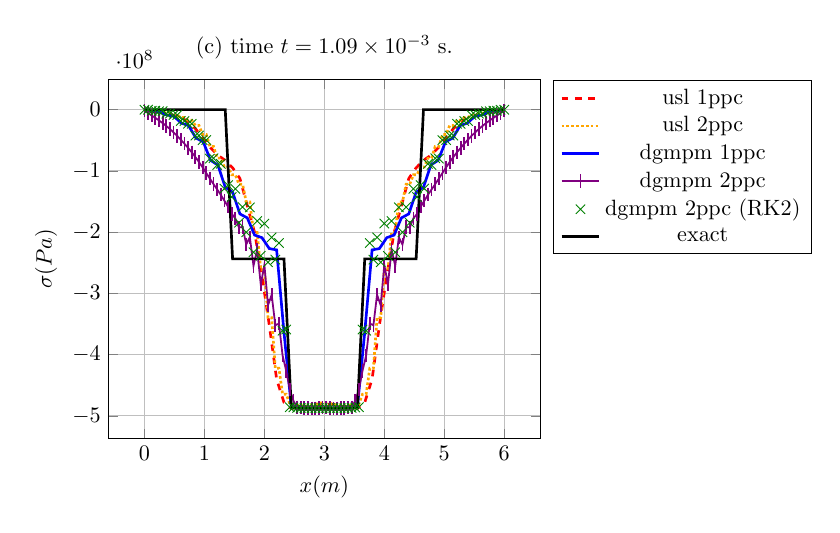
\begin{tikzpicture}[scale=0.8]
\begin{axis}[xlabel=$x (m)$,ylabel=$\sigma (Pa)$,ymajorgrids=true,xmajorgrids=true,legend pos=outer north east,title={(c) time $t = 1.09\times 10^{-3} $ s.}]
\addplot[Red,very thick,mark=none,dashed,mark size=3pt] coordinates {(0.0,-679166.0601331755) (0.12244897959183673,-2368189.594188208) (0.24489795918367346,-4606456.556212341) (0.36734693877551017,-6961578.395676694) (0.4897959183673469,-9332760.287028607) (0.6122448979591837,-12938682.464591796) (0.7346938775510203,-20102821.471402142) (0.8571428571428571,-32015823.341737133) (0.9795918367346939,-47676454.15860757) (1.1020408163265305,-62502940.42234602) (1.2244897959183674,-74544680.06037714) (1.346938775510204,-82775603.38522142) (1.4693877551020407,-94947363.4179823) (1.5918367346938775,-112415785.44002911) (1.7142857142857142,-156774491.63523546) (1.836734693877551,-200654618.50473383) (1.9591836734693877,-270646588.3413816) (2.0816326530612246,-351928629.9311485) (2.204081632653061,-440064160.15512294) (2.326530612244898,-477934424.91056436) (2.4489795918367347,-487815276.0764712) (2.571428571428571,-485351241.33413374) (2.693877551020408,-484406188.97201383) (2.816326530612245,-481035531.7602433) (2.9387755102040813,-481038509.8228564) (3.061224489795918,-481038509.8228558) (3.183673469387755,-481035531.7602443) (3.306122448979592,-484406188.9720135) (3.4285714285714284,-485351241.3341341) (3.5510204081632653,-487815276.07647014) (3.673469387755102,-477934424.9105651) (3.7959183673469385,-440064160.15512156) (3.9183673469387754,-351928629.931148) (4.040816326530612,-270646588.34138024) (4.163265306122449,-200654618.50473374) (4.285714285714286,-156774491.63523474) (4.408163265306122,-112415785.44002907) (4.530612244897959,-94947363.41798277) (4.653061224489796,-82775603.38522187) (4.775510204081632,-74544680.06037733) (4.8979591836734695,-62502940.42234604) (5.020408163265306,-47676454.158607304) (5.142857142857142,-32015823.341736842) (5.26530612244898,-20102821.471402) (5.387755102040816,-12938682.46459166) (5.5102040816326525,-9332760.287028512) (5.63265306122449,-6961578.395676572) (5.755102040816326,-4606456.55621225) (5.877551020408163,-2368189.594188123) (6.0,-679166.0601331636) };
\addplot[Orange,very thick,mark=none,densely dotted,mark size=3pt] coordinates {(0.0,-512829.37356199906) (0.06060606060606061,-512829.37356199906) (0.12121212121212122,-1685977.6907792736) (0.18181818181818182,-1685977.6907792736) (0.24242424242424243,-3409631.957049818) (0.30303030303030304,-3409631.957049818) (0.36363636363636365,-5994518.467970753) (0.42424242424242425,-5994518.467970753) (0.48484848484848486,-9186608.055434104) (0.5454545454545454,-9186608.055434104) (0.6060606060606061,-12632033.888351096) (0.6666666666666667,-12632033.888351096) (0.7272727272727273,-17308370.109125804) (0.7878787878787878,-17308370.109125804) (0.8484848484848485,-25927147.931033082) (0.9090909090909092,-25927147.931033082) (0.9696969696969697,-40719694.7337496) (1.0303030303030303,-40719694.7337496) (1.0909090909090908,-60222421.752752535) (1.1515151515151516,-60222421.752752535) (1.2121212121212122,-79232798.7243564) (1.2727272727272727,-79232798.7243564) (1.3333333333333335,-93917910.36545579) (1.393939393939394,-93917910.36545579) (1.4545454545454546,-106296964.05562654) (1.5151515151515151,-106296964.05562654) (1.5757575757575757,-121857025.50296684) (1.6363636363636365,-121857025.50296684) (1.696969696969697,-150591571.19633642) (1.7575757575757576,-150591571.19633642) (1.8181818181818183,-200655220.68880683) (1.878787878787879,-200655220.68880683) (1.9393939393939394,-261493503.50548327) (2.0,-261493503.50548327) (2.0606060606060606,-339524928.63039523) (2.121212121212121,-339524928.63039523) (2.1818181818181817,-422131801.353524) (2.2424242424242427,-422131801.353524) (2.303030303030303,-464494091.2915379) (2.3636363636363638,-464494091.2915379) (2.4242424242424243,-480288801.84594995) (2.484848484848485,-480288801.84594995) (2.5454545454545454,-482971319.0696361) (2.606060606060606,-482971319.0696361) (2.666666666666667,-484006263.5397973) (2.7272727272727275,-484006263.5397973) (2.787878787878788,-481823971.2401126) (2.8484848484848486,-481823971.2401126) (2.909090909090909,-478820708.8588188) (2.9696969696969697,-478820708.8588188) (3.0303030303030303,-478820708.8588188) (3.090909090909091,-478820708.8588188) (3.1515151515151514,-481823971.24011296) (3.2121212121212124,-481823971.24011296) (3.272727272727273,-484006263.53979766) (3.3333333333333335,-484006263.53979766) (3.393939393939394,-482971319.0696361) (3.4545454545454546,-482971319.0696361) (3.515151515151515,-480288801.84594995) (3.5757575757575757,-480288801.84594995) (3.6363636363636367,-464494091.2915379) (3.6969696969696972,-464494091.2915379) (3.757575757575758,-422131801.3535244) (3.8181818181818183,-422131801.3535244) (3.878787878787879,-339524928.6303949) (3.9393939393939394,-339524928.6303949) (4.0,-261493503.50548312) (4.0606060606060606,-261493503.50548312) (4.121212121212121,-200655220.68880683) (4.181818181818182,-200655220.68880683) (4.242424242424242,-150591571.1963363) (4.303030303030303,-150591571.1963363) (4.363636363636363,-121857025.50296697) (4.424242424242425,-121857025.50296697) (4.484848484848485,-106296964.05562642) (4.545454545454546,-106296964.05562642) (4.606060606060606,-93917910.36545563) (4.666666666666667,-93917910.36545563) (4.7272727272727275,-79232798.7243563) (4.787878787878788,-79232798.7243563) (4.848484848484849,-60222421.752752505) (4.909090909090909,-60222421.752752505) (4.96969696969697,-40719694.73374956) (5.03030303030303,-40719694.73374956) (5.090909090909091,-25927147.93103303) (5.151515151515151,-25927147.93103303) (5.212121212121212,-17308370.109125733) (5.2727272727272725,-17308370.109125733) (5.333333333333334,-12632033.888351053) (5.3939393939393945,-12632033.888351053) (5.454545454545455,-9186608.05543412) (5.515151515151516,-9186608.05543412) (5.575757575757576,-5994518.467970843) (5.636363636363637,-5994518.467970843) (5.696969696969697,-3409631.957049952) (5.757575757575758,-3409631.957049952) (5.818181818181818,-1685977.690779395) (5.878787878787879,-1685977.690779395) (5.9393939393939394,-512829.37356205017) (6.0,-512829.37356205017) };
\addplot[Blue,very thick,mark=none,solid,mark size=3pt] coordinates {(0.0,-298852.1952411225) (0.12244897959183673,-2592980.4740912793) (0.24489795918367346,-3560236.4322381816) (0.36734693877551017,-8652722.221047912) (0.4897959183673469,-10777216.673686886) (0.6122448979591837,-21974314.707157355) (0.7346938775510203,-26009924.918005344) (0.8571428571428571,-46347563.10657899) (0.9795918367346939,-52593345.171819046) (1.1020408163265305,-82683979.65035231) (1.2244897959183674,-90525380.97285904) (1.346938775510204,-126773557.44849168) (1.4693877551020407,-134743667.28836828) (1.5918367346938775,-170219249.4978279) (1.7142857142857142,-176744937.7749974) (1.836734693877551,-204799464.24688196) (1.9591836734693877,-209064122.25232974) (2.0816326530612246,-226820170.49378502) (2.204081632653061,-229011964.3130221) (2.326530612244898,-363270795.9137317) (2.4489795918367347,-485529213.90073514) (2.571428571428571,-486748760.1951447) (2.693877551020408,-487164866.56783277) (2.816326530612245,-487268871.16624963) (2.9387755102040813,-487285807.7274521) (3.061224489795918,-487285807.7274521) (3.183673469387755,-487268871.16624963) (3.306122448979592,-487164866.56783277) (3.4285714285714284,-486748760.1951447) (3.5510204081632653,-485529213.90073514) (3.673469387755102,-363270795.91372997) (3.7959183673469385,-229011964.3130223) (3.9183673469387754,-226820170.49378502) (4.040816326530612,-209064122.25232938) (4.163265306122449,-204799464.2468816) (4.285714285714286,-176744937.77499697) (4.408163265306122,-170219249.4978276) (4.530612244897959,-134743667.28836808) (4.653061224489796,-126773557.44849148) (4.775510204081632,-90525380.9728589) (4.8979591836734695,-82683979.65035222) (5.020408163265306,-52593345.171819076) (5.142857142857142,-46347563.10657902) (5.26530612244898,-26009924.918005634) (5.387755102040816,-21974314.707157686) (5.5102040816326525,-10777216.673687106) (5.63265306122449,-8652722.22104813) (5.755102040816326,-3560236.4322383474) (5.877551020408163,-2592980.4740913147) (6.0,-298852.1952412414) };
\addplot[Purple,thick,mark=|,solid,mark size=3pt] coordinates {(0.0,-1967506.1700863338) (0.06060606060606061,-5640032.662143143) (0.12121212121212122,-9656978.414919749) (0.18181818181818182,-13511820.529648876) (0.24242424242424243,-17791285.14768848) (0.30303030303030304,-22020954.760085706) (0.36363636363636365,-26810841.63481511) (0.42424242424242425,-31669769.847401485) (0.48484848484848486,-37219038.25874583) (0.5454545454545454,-42898302.86376866) (0.6060606060606061,-49215331.978578255) (0.6666666666666667,-55631508.92977342) (0.7272727272727273,-62575105.835719146) (0.7878787878787878,-69650368.30460997) (0.8484848484848485,-77440912.11382866) (0.9090909090909092,-85513317.74757525) (0.9696969696969697,-94394406.18118168) (1.0303030303030303,-103458727.33292748) (1.0909090909090908,-112622821.36245859) (1.1515151515151516,-121624138.89888178) (1.2121212121212122,-130341670.55898608) (1.2727272727272727,-139154542.84528217) (1.3333333333333335,-148830679.63128546) (1.393939393939394,-158542307.8017911) (1.4545454545454546,-170175255.01202118) (1.5151515151515151,-177512130.9706464) (1.5757575757575757,-192468554.83417034) (1.6363636363636365,-191410973.67950493) (1.696969696969697,-220188643.16229337) (1.7575757575757576,-208348179.3812332) (1.8181818181818183,-255105244.69638902) (1.878787878787879,-228761423.37895402) (1.9393939393939394,-285472179.8898197) (2.0,-253525121.96460363) (2.0606060606060606,-319389070.9725514) (2.121212121212121,-302097367.51271814) (2.1818181818181817,-351940004.91030246) (2.2424242424242427,-349259097.20874596) (2.303030303030303,-401088439.8898511) (2.3636363636363638,-426445036.100153) (2.4242424242424243,-456776041.9007156) (2.484848484848485,-475327504.30100346) (2.5454545454545454,-485932720.49084026) (2.606060606060606,-486800863.6836889) (2.666666666666667,-487206914.08181626) (2.7272727272727275,-487221866.2556566) (2.787878787878788,-487293102.56783485) (2.8484848484848486,-487291983.48275816) (2.909090909090909,-486820130.2994909) (2.9696969696969697,-486154460.1484115) (3.0303030303030303,-486154460.1484115) (3.090909090909091,-486820130.2994909) (3.1515151515151514,-487291983.4827589) (3.2121212121212124,-487293102.56783485) (3.272727272727273,-487221866.2556566) (3.3333333333333335,-487206914.08181626) (3.393939393939394,-486800863.68368924) (3.4545454545454546,-485932720.4908413) (3.515151515151515,-475327504.30100375) (3.5757575757575757,-456776041.90071523) (3.6363636363636367,-426445036.10015374) (3.6969696969696972,-401088439.8898514) (3.757575757575758,-349259097.2087466) (3.8181818181818183,-351940004.91030276) (3.878787878787879,-302097367.5127176) (3.9393939393939394,-319389070.9725512) (4.0,-253525121.96460345) (4.0606060606060606,-285472179.8898196) (4.121212121212121,-228761423.3789541) (4.181818181818182,-255105244.69638902) (4.242424242424242,-208348179.3812334) (4.303030303030303,-220188643.16229364) (4.363636363636363,-191410973.6795053) (4.424242424242425,-192468554.83417064) (4.484848484848485,-177512130.97064662) (4.545454545454546,-170175255.01202148) (4.606060606060606,-158542307.8017913) (4.666666666666667,-148830679.63128573) (4.7272727272727275,-139154542.84528223) (4.787878787878788,-130341670.55898641) (4.848484848484849,-121624138.89888197) (4.909090909090909,-112622821.36245887) (4.96969696969697,-103458727.33292772) (5.03030303030303,-94394406.18118192) (5.090909090909091,-85513317.74757543) (5.151515151515151,-77440912.11382888) (5.212121212121212,-69650368.30461016) (5.2727272727272725,-62575105.83571933) (5.333333333333334,-55631508.92977359) (5.3939393939393945,-49215331.97857844) (5.454545454545455,-42898302.863768816) (5.515151515151516,-37219038.25874599) (5.575757575757576,-31669769.847401626) (5.636363636363637,-26810841.634815253) (5.696969696969697,-22020954.760085825) (5.757575757575758,-17791285.147688594) (5.818181818181818,-13511820.529648978) (5.878787878787879,-9656978.414919829) (5.9393939393939394,-5640032.662143192) (6.0,-1967506.1700863515) };
\addplot[Green,thin,mark=x,only marks,mark size=3pt] coordinates {(0.0,-230769.40948159585) (0.06060606060606061,-230768.71951221325) (0.12121212121212122,-1765050.39034623) (0.18181818181818182,-1765048.7256776437) (0.24242424242424243,-2617614.5488237087) (0.30303030303030304,-2617595.5576229785) (0.36363636363636365,-6618855.725385412) (0.42424242424242425,-6618791.381126346) (0.48484848484848486,-8782768.896716146) (0.5454545454545454,-8782347.865813052) (0.6060606060606061,-18621957.945415) (0.6666666666666667,-18620353.83429409) (0.7272727272727273,-23151239.305377506) (0.7878787878787878,-23143055.39749537) (0.8484848484848485,-42429548.36143795) (0.9090909090909092,-42396573.934735104) (0.9696969696969697,-49952758.0967802) (1.0303030303030303,-49806565.98801953) (1.0909090909090908,-80012587.42975214) (1.1515151515151516,-79461376.35879174) (1.2121212121212122,-90415119.5727169) (1.2727272727272727,-88488293.78873543) (1.3333333333333335,-128889020.76572785) (1.393939393939394,-123386634.02232555) (1.4545454545454546,-142761259.00417286) (1.5151515151515151,-129449157.87721576) (1.5757575757575757,-184648477.15027985) (1.6363636363636365,-158996250.14018014) (1.696969696969697,-200285677.94521412) (1.7575757575757576,-159431830.86237475) (1.8181818181818183,-232788597.47549) (1.878787878787879,-181815073.16887435) (1.9393939393939394,-238716756.27113715) (2.0,-185991644.81247783) (2.0606060606060606,-249108768.01695433) (2.121212121212121,-208608151.93422446) (2.1818181818181817,-244796764.89630747) (2.2424242424242427,-217807407.36442074) (2.303030303030303,-360926830.0819958) (2.3636363636363638,-358951385.7834185) (2.4242424242424243,-485803376.4944678) (2.484848484848485,-486055584.43364054) (2.5454545454545454,-486867155.31944156) (2.606060606060606,-486947986.92719907) (2.666666666666667,-487200286.73057413) (2.7272727272727275,-487218951.17205155) (2.787878787878788,-487275506.6886281) (2.8484848484848486,-487278268.04119205) (2.909090909090909,-487286397.423194) (2.9696969696969697,-487286593.83864176) (3.0303030303030303,-487286593.83864176) (3.090909090909091,-487286397.423194) (3.1515151515151514,-487278268.04119205) (3.2121212121212124,-487275506.6886281) (3.272727272727273,-487218951.17205155) (3.3333333333333335,-487200286.73057413) (3.393939393939394,-486947986.92719907) (3.4545454545454546,-486867155.31944156) (3.515151515151515,-486055584.43364054) (3.5757575757575757,-485803376.4944678) (3.6363636363636367,-358951385.78341883) (3.6969696969696972,-360926830.08199614) (3.757575757575758,-217807407.3644211) (3.8181818181818183,-244796764.896308) (3.878787878787879,-208608151.93422586) (3.9393939393939394,-249108768.01695573) (4.0,-185991644.81247783) (4.0606060606060606,-238716756.27113697) (4.121212121212121,-181815073.16887408) (4.181818181818182,-232788597.47549027) (4.242424242424242,-159431830.86237472) (4.303030303030303,-200285677.9452144) (4.363636363636363,-158996250.1401801) (4.424242424242425,-184648477.15027985) (4.484848484848485,-129449157.87721583) (4.545454545454546,-142761259.0041731) (4.606060606060606,-123386634.02232562) (4.666666666666667,-128889020.76572803) (4.7272727272727275,-88488293.78873555) (4.787878787878788,-90415119.57271707) (4.848484848484849,-79461376.35879163) (4.909090909090909,-80012587.42975211) (4.96969696969697,-49806565.98801959) (5.03030303030303,-49952758.096780345) (5.090909090909091,-42396573.93473512) (5.151515151515151,-42429548.36143816) (5.212121212121212,-23143055.397495314) (5.2727272727272725,-23151239.305377506) (5.333333333333334,-18620353.834293906) (5.3939393939393945,-18621957.94541511) (5.454545454545455,-8782347.865813203) (5.515151515151516,-8782768.896716148) (5.575757575757576,-6618791.38112651) (5.636363636363637,-6618855.725385466) (5.696969696969697,-2617595.5576235284) (5.757575757575758,-2617614.5488236495) (5.818181818181818,-1765048.7256772814) (5.878787878787879,-1765050.390346396) (5.9393939393939394,-230768.71951233502) (6.0,-230769.4094818794) };
\addplot[black,very thick,mark=pentagone*,solid,mark size=3pt] coordinates {(0.0,-0.0) (0.12244897959183673,-0.0) (0.24489795918367346,-0.0) (0.36734693877551017,-0.0) (0.4897959183673469,-0.0) (0.6122448979591837,-0.0) (0.7346938775510203,-0.0) (0.8571428571428571,-0.0) (0.9795918367346939,-0.0) (1.1020408163265305,-0.0) (1.2244897959183674,-0.0) (1.346938775510204,-0.0) (1.4693877551020407,-243643578.04719847) (1.5918367346938775,-243643578.04719847) (1.7142857142857142,-243643578.04719847) (1.836734693877551,-243643578.04719847) (1.9591836734693877,-243643578.04719847) (2.0816326530612246,-243643578.04719847) (2.204081632653061,-243643578.04719847) (2.326530612244898,-243643578.04719847) (2.4489795918367347,-487287156.09439695) (2.571428571428571,-487287156.09439695) (2.693877551020408,-487287156.09439695) (2.816326530612245,-487287156.09439695) (2.9387755102040813,-487287156.09439695) (3.061224489795918,-487287156.09439695) (3.183673469387755,-487287156.09439695) (3.306122448979592,-487287156.09439695) (3.4285714285714284,-487287156.09439695) (3.5510204081632653,-487287156.09439695) (3.673469387755102,-243643578.04719847) (3.7959183673469385,-243643578.04719847) (3.9183673469387754,-243643578.04719847) (4.040816326530612,-243643578.04719847) (4.163265306122449,-243643578.04719847) (4.285714285714286,-243643578.04719847) (4.408163265306122,-243643578.04719847) (4.530612244897959,-243643578.04719847) (4.653061224489796,-0.0) (4.775510204081632,-0.0) (4.8979591836734695,-0.0) (5.020408163265306,-0.0) (5.142857142857142,-0.0) (5.26530612244898,-0.0) (5.387755102040816,-0.0) (5.5102040816326525,-0.0) (5.63265306122449,-0.0) (5.755102040816326,-0.0) (5.877551020408163,-0.0) (6.0,-0.0) };
\legend{usl 1ppc,usl 2ppc,dgmpm 1ppc,dgmpm 2ppc,dgmpm 2ppc (RK2),exact}
\end{axis}
\end{tikzpicture}
%%% Local Variables:
%%% mode: latex
%%% TeX-master: "../../mainManuscript"
%%% End:
}
%   \caption{elastic-plastic RP stress}
%   \label{fig:stress_elastoplastic_RP}
% \end{figure}
% \begin{figure}[h!]
%   \centering
%   {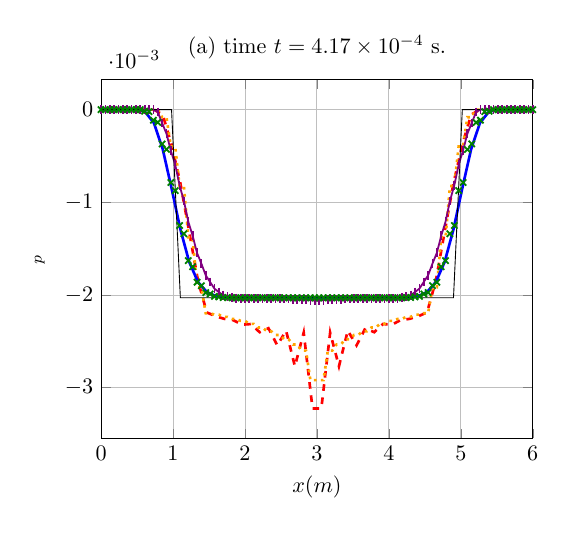
\begin{tikzpicture}[scale=0.8]
\begin{axis}[xlabel=$x (m)$,ylabel=$\eps^p$,ymajorgrids=true,xmajorgrids=true,legend pos=outer north east,title={(a) time $t = 4.17\times 10^{-4} $ s.},xmin=0.,xmax=6.]
\addplot[Red,very thick,mark=none,dashed] coordinates {(0.0,0.0) (0.12244897959183673,0.0) (0.24489795918367346,0.0) (0.36734693877551017,0.0) (0.4897959183673469,0.0) (0.6122448979591837,0.0) (0.7346938775510203,0.0) (0.8571428571428571,-5.5177825258810104e-05) (0.9795918367346939,-0.0003791196239632164) (1.1020408163265305,-0.0007942218458547296) (1.2244897959183674,-0.0013158519965027296) (1.346938775510204,-0.0018458090676901286) (1.4693877551020407,-0.002188794617508559) (1.5918367346938775,-0.002229697455331896) (1.7142857142857142,-0.002258121963594508) (1.836734693877551,-0.002271799079674154) (1.9591836734693877,-0.002320613632318322) (2.0816326530612246,-0.002313868472160546) (2.204081632653061,-0.0024020122032007017) (2.326530612244898,-0.0023588630990294623) (2.4489795918367347,-0.0025433455597807667) (2.571428571428571,-0.002385435935351422) (2.693877551020408,-0.0027693350417516906) (2.816326530612245,-0.0024065265204776445) (2.9387755102040813,-0.0032250612006492966) (3.061224489795918,-0.0032250612006492524) (3.183673469387755,-0.002406526520477666) (3.306122448979592,-0.0027693350417516823) (3.4285714285714284,-0.0023854359353514295) (3.5510204081632653,-0.0025433455597807628) (3.673469387755102,-0.002358863099029464) (3.7959183673469385,-0.0024020122032006983) (3.9183673469387754,-0.0023138684721605448) (4.040816326530612,-0.002320613632318319) (4.163265306122449,-0.0022717990796741546) (4.285714285714286,-0.0022581219635945077) (4.408163265306122,-0.0022296974553318956) (4.530612244897959,-0.0021887946175085595) (4.653061224489796,-0.001845809067690125) (4.775510204081632,-0.0013158519965027254) (4.8979591836734695,-0.0007942218458547295) (5.020408163265306,-0.0003791196239632123) (5.142857142857142,-5.5177825258808404e-05) (5.26530612244898,0.0) (5.387755102040816,0.0) (5.5102040816326525,0.0) (5.63265306122449,0.0) (5.755102040816326,0.0) (5.877551020408163,0.0) (6.0,0.0) };
\addplot[Orange,very thick,mark=none,dotted] coordinates {(0.0,0.0) (0.06060606060606061,0.0) (0.12121212121212122,0.0) (0.18181818181818182,0.0) (0.24242424242424243,0.0) (0.30303030303030304,0.0) (0.36363636363636365,0.0) (0.42424242424242425,0.0) (0.48484848484848486,0.0) (0.5454545454545454,0.0) (0.6060606060606061,0.0) (0.6666666666666667,0.0) (0.7272727272727273,0.0) (0.7878787878787878,0.0) (0.8484848484848485,-8.276994982638746e-05) (0.9090909090909092,-8.276994982638746e-05) (0.9696969696969697,-0.0003982743796454725) (1.0303030303030303,-0.0003982743796454725) (1.0909090909090908,-0.0008251664654092959) (1.1515151515151516,-0.0008251664654092959) (1.2121212121212122,-0.0013769280756316814) (1.2727272727272727,-0.0013769280756316814) (1.3333333333333335,-0.0019184552821342453) (1.393939393939394,-0.0019184552821342453) (1.4545454545454546,-0.0021968313010739355) (1.5151515151515151,-0.0021968313010739355) (1.5757575757575757,-0.0022123334205993417) (1.6363636363636365,-0.0022123334205993417) (1.696969696969697,-0.0022365941606657474) (1.7575757575757576,-0.0022365941606657474) (1.8181818181818183,-0.0022585940891309796) (1.878787878787879,-0.0022585940891309796) (1.9393939393939394,-0.0022798424574663194) (2.0,-0.0022798424574663194) (2.0606060606060606,-0.0023117041253564387) (2.121212121212121,-0.0023117041253564387) (2.1818181818181817,-0.002350782112768782) (2.2424242424242427,-0.002350782112768782) (2.303030303030303,-0.002390940396871615) (2.3636363636363638,-0.002390940396871615) (2.4242424242424243,-0.0024313395034050904) (2.484848484848485,-0.0024313395034050904) (2.5454545454545454,-0.002477563584428502) (2.606060606060606,-0.002477563584428502) (2.666666666666667,-0.0025344573000873694) (2.7272727272727275,-0.0025344573000873694) (2.787878787878788,-0.002600834768573611) (2.8484848484848486,-0.002600834768573611) (2.909090909090909,-0.0029191565184019295) (2.9696969696969697,-0.0029191565184019295) (3.0303030303030303,-0.0029191565184019273) (3.090909090909091,-0.0029191565184019273) (3.1515151515151514,-0.0026008347685736143) (3.2121212121212124,-0.0026008347685736143) (3.272727272727273,-0.002534457300087371) (3.3333333333333335,-0.002534457300087371) (3.393939393939394,-0.0024775635844285025) (3.4545454545454546,-0.0024775635844285025) (3.515151515151515,-0.0024313395034050896) (3.5757575757575757,-0.0024313395034050896) (3.6363636363636367,-0.002390940396871615) (3.6969696969696972,-0.002390940396871615) (3.757575757575758,-0.0023507821127687826) (3.8181818181818183,-0.0023507821127687826) (3.878787878787879,-0.002311704125356438) (3.9393939393939394,-0.002311704125356438) (4.0,-0.0022798424574663172) (4.0606060606060606,-0.0022798424574663172) (4.121212121212121,-0.00225859408913098) (4.181818181818182,-0.00225859408913098) (4.242424242424242,-0.002236594160665746) (4.303030303030303,-0.002236594160665746) (4.363636363636363,-0.0022123334205993426) (4.424242424242425,-0.0022123334205993426) (4.484848484848485,-0.002196831301073935) (4.545454545454546,-0.002196831301073935) (4.606060606060606,-0.0019184552821342445) (4.666666666666667,-0.0019184552821342445) (4.7272727272727275,-0.0013769280756316814) (4.787878787878788,-0.0013769280756316814) (4.848484848484849,-0.0008251664654092957) (4.909090909090909,-0.0008251664654092957) (4.96969696969697,-0.0003982743796454725) (5.03030303030303,-0.0003982743796454725) (5.090909090909091,-8.276994982638697e-05) (5.151515151515151,-8.276994982638697e-05) (5.212121212121212,0.0) (5.2727272727272725,0.0) (5.333333333333334,0.0) (5.3939393939393945,0.0) (5.454545454545455,0.0) (5.515151515151516,0.0) (5.575757575757576,0.0) (5.636363636363637,0.0) (5.696969696969697,0.0) (5.757575757575758,0.0) (5.818181818181818,0.0) (5.878787878787879,0.0) (5.9393939393939394,0.0) (6.0,0.0) };
\addplot[Blue,very thick,mark=none,solid] coordinates {(0.0,0.0) (0.12244897959183673,0.0) (0.24489795918367346,0.0) (0.36734693877551017,0.0) (0.4897959183673469,0.0) (0.6122448979591837,-2.4267855226065594e-05) (0.7346938775510203,-0.00014452073597361284) (0.8571428571428571,-0.0004275642401009131) (0.9795918367346939,-0.0008483282066457896) (1.1020408163265305,-0.0012913872123487611) (1.2244897959183674,-0.001642660920094959) (1.346938775510204,-0.0018602413103573651) (1.4693877551020407,-0.0019680574666657586) (1.5918367346938775,-0.00201146561977191) (1.7142857142857142,-0.002025805454394895) (1.836734693877551,-0.0020297136017104972) (1.9591836734693877,-0.002030593864489664) (2.0816326530612246,-0.002030757436013639) (2.204081632653061,-0.0020307823755532774) (2.326530612244898,-0.002030785465084119) (2.4489795918367347,-0.0020307857712710334) (2.571428571428571,-0.00203078579497771) (2.693877551020408,-0.0020307857963597366) (2.816326530612245,-0.002030785796416807) (2.9387755102040813,-0.002030785796418294) (3.061224489795918,-0.002030785796418294) (3.183673469387755,-0.0020307857964168056) (3.306122448979592,-0.002030785796359739) (3.4285714285714284,-0.0020307857949777124) (3.5510204081632653,-0.002030785771271032) (3.673469387755102,-0.002030785465084119) (3.7959183673469385,-0.002030782375553277) (3.9183673469387754,-0.0020307574360136386) (4.040816326530612,-0.002030593864489664) (4.163265306122449,-0.0020297136017104964) (4.285714285714286,-0.0020258054543948927) (4.408163265306122,-0.002011465619771909) (4.530612244897959,-0.0019680574666657573) (4.653061224489796,-0.0018602413103573651) (4.775510204081632,-0.0016426609200949592) (4.8979591836734695,-0.001291387212348762) (5.020408163265306,-0.0008483282066457893) (5.142857142857142,-0.00042756424010091193) (5.26530612244898,-0.00014452073597361384) (5.387755102040816,-2.4267855226067292e-05) (5.5102040816326525,0.0) (5.63265306122449,0.0) (5.755102040816326,0.0) (5.877551020408163,0.0) (6.0,0.0) };
\addplot[Purple,thick,mark=|,solid] coordinates {(0.0,0.0) (0.06060606060606061,0.0) (0.12121212121212122,0.0) (0.18181818181818182,0.0) (0.24242424242424243,0.0) (0.30303030303030304,0.0) (0.36363636363636365,0.0) (0.42424242424242425,0.0) (0.48484848484848486,0.0) (0.5454545454545454,0.0) (0.6060606060606061,0.0) (0.6666666666666667,0.0) (0.7272727272727273,0.0) (0.7878787878787878,-2.5923316540887583e-05) (0.8484848484848485,-0.00014408338164523062) (0.9090909090909092,-0.00026064821701688356) (0.9696969696969697,-0.00044254060540111623) (1.0303030303030303,-0.0005942249623309128) (1.0909090909090908,-0.0008176542805902086) (1.1515151515151516,-0.0009856283620753997) (1.2121212121212122,-0.0012081222038318737) (1.2727272727272727,-0.001361479798176913) (1.3333333333333335,-0.0015454861370016277) (1.393939393939394,-0.0016614769826446604) (1.4545454545454546,-0.001787668142599641) (1.5151515151515151,-0.0018601100018299035) (1.5757575757575757,-0.0019316233200168077) (1.6363636363636365,-0.0019687068201561) (1.696969696969697,-0.0020017521579713225) (1.7575757575757576,-0.002016983208079143) (1.8181818181818183,-0.0020290662590489866) (1.878787878787879,-0.002033836939779926) (1.9393939393939394,-0.002037035363641218) (2.0,-0.002037968116126088) (2.0606060606060606,-0.0020383611759408468) (2.121212121212121,-0.002038518677096413) (2.1818181818181817,-0.0020388624173375575) (2.2424242424242427,-0.002039197521601926) (2.303030303030303,-0.0020400227446406255) (2.3636363636363638,-0.0020406530704546125) (2.4242424242424243,-0.0020416018700111314) (2.484848484848485,-0.00204214484166886) (2.5454545454545454,-0.002043028167195094) (2.606060606060606,-0.0020436145435565973) (2.666666666666667,-0.0020449363268448036) (2.7272727272727275,-0.0020459859423928813) (2.787878787878788,-0.002048543419164452) (2.8484848484848486,-0.002051015793534283) (2.909090909090909,-0.0020569476212071243) (2.9696969696969697,-0.0020621904992435833) (3.0303030303030303,-0.0020621904992435824) (3.090909090909091,-0.002056947621207125) (3.1515151515151514,-0.0020510157935342823) (3.2121212121212124,-0.002048543419164453) (3.272727272727273,-0.0020459859423928826) (3.3333333333333335,-0.0020449363268448045) (3.393939393939394,-0.0020436145435565965) (3.4545454545454546,-0.002043028167195095) (3.515151515151515,-0.0020421448416688593) (3.5757575757575757,-0.002041601870011131) (3.6363636363636367,-0.00204065307045461) (3.6969696969696972,-0.0020400227446406246) (3.757575757575758,-0.0020391975216019266) (3.8181818181818183,-0.002038862417337557) (3.878787878787879,-0.002038518677096414) (3.9393939393939394,-0.0020383611759408476) (4.0,-0.0020379681161260864) (4.0606060606060606,-0.0020370353636412174) (4.121212121212121,-0.002033836939779926) (4.181818181818182,-0.0020290662590489866) (4.242424242424242,-0.0020169832080791424) (4.303030303030303,-0.0020017521579713243) (4.363636363636363,-0.0019687068201561025) (4.424242424242425,-0.0019316233200168081) (4.484848484848485,-0.0018601100018299066) (4.545454545454546,-0.0017876681425996446) (4.606060606060606,-0.0016614769826446619) (4.666666666666667,-0.00154548613700163) (4.7272727272727275,-0.0013614797981769142) (4.787878787878788,-0.001208122203831875) (4.848484848484849,-0.0009856283620754) (4.909090909090909,-0.0008176542805902103) (4.96969696969697,-0.0005942249623309133) (5.03030303030303,-0.0004425406054011171) (5.090909090909091,-0.0002606482170168828) (5.151515151515151,-0.0001440833816452316) (5.212121212121212,-2.5923316540887827e-05) (5.2727272727272725,0.0) (5.333333333333334,0.0) (5.3939393939393945,0.0) (5.454545454545455,0.0) (5.515151515151516,0.0) (5.575757575757576,0.0) (5.636363636363637,0.0) (5.696969696969697,0.0) (5.757575757575758,0.0) (5.818181818181818,0.0) (5.878787878787879,0.0) (5.9393939393939394,0.0) (6.0,0.0) };
\addplot[Green,thick,mark=x,only marks] coordinates {(0.0,0.0) (0.06060606060606061,0.0) (0.12121212121212122,0.0) (0.18181818181818182,0.0) (0.24242424242424243,0.0) (0.30303030303030304,0.0) (0.36363636363636365,0.0) (0.42424242424242425,0.0) (0.48484848484848486,0.0) (0.5454545454545454,0.0) (0.6060606060606061,-1.7121600888926267e-05) (0.6666666666666667,-2.172686744419618e-05) (0.7272727272727273,-0.00011443767993769938) (0.7878787878787878,-0.00013866917764854026) (0.8484848484848485,-0.000370837449450201) (0.9090909090909092,-0.00042969060271589064) (0.9696969696969697,-0.0007865101118856191) (1.0303030303030303,-0.0008740536663337508) (1.0909090909090908,-0.0012506750549991495) (1.1515151515151516,-0.0013398986968958142) (1.2121212121212122,-0.001629336049869835) (1.2727272727272727,-0.0016953745726422953) (1.3333333333333335,-0.0018628910299540863) (1.393939393939394,-0.001899592623043941) (1.4545454545454546,-0.0019740737222564337) (1.5151515151515151,-0.001989690337719905) (1.5757575757575757,-0.0020154070144030914) (1.6363636363636365,-0.002020547105162428) (1.696969696969697,-0.00202746624770192) (1.7575757575757576,-0.0020287782703279386) (1.8181818181818183,-0.002030222920814726) (1.878787878787879,-0.0020304811945086915) (1.9393939393939394,-0.0020307137632274313) (2.0,-0.002030752789922547) (2.0606060606060606,-0.0020307781606480066) (2.121212121212121,-0.002030781734154242) (2.1818181818181817,-0.0020307845358815933) (2.2424242424242427,-0.002030784913407357) (2.303030303030303,-0.002030786093815172) (2.3636363636363638,-0.0020307883320914285) (2.4242424242424243,-0.0020307890300132712) (2.484848484848485,-0.0020307901307202374) (2.5454545454545454,-0.002030792281554236) (2.606060606060606,-0.002030795453324907) (2.666666666666667,-0.0020307979071881566) (2.7272727272727275,-0.0020308065650964362) (2.787878787878788,-0.002030816863285245) (2.8484848484848486,-0.0020308137021312345) (2.909090909090909,-0.0020308908094497746) (2.9696969696969697,-0.002031166801141057) (3.0303030303030303,-0.0020311668011410568) (3.090909090909091,-0.002030890809449775) (3.1515151515151514,-0.002030813702131235) (3.2121212121212124,-0.002030816863285247) (3.272727272727273,-0.002030806565096435) (3.3333333333333335,-0.0020307979071881553) (3.393939393939394,-0.0020307954533249043) (3.4545454545454546,-0.0020307922815542352) (3.515151515151515,-0.0020307901307202374) (3.5757575757575757,-0.0020307890300132712) (3.6363636363636367,-0.00203078833209143) (3.6969696969696972,-0.0020307860938151728) (3.757575757575758,-0.002030784913407359) (3.8181818181818183,-0.002030784535881596) (3.878787878787879,-0.0020307817341542406) (3.9393939393939394,-0.0020307781606480053) (4.0,-0.0020307527899225478) (4.0606060606060606,-0.0020307137632274313) (4.121212121212121,-0.002030481194508689) (4.181818181818182,-0.0020302229208147243) (4.242424242424242,-0.0020287782703279416) (4.303030303030303,-0.0020274662477019227) (4.363636363636363,-0.002020547105162427) (4.424242424242425,-0.002015407014403091) (4.484848484848485,-0.0019896903377199055) (4.545454545454546,-0.001974073722256437) (4.606060606060606,-0.0018995926230439425) (4.666666666666667,-0.0018628910299540889) (4.7272727272727275,-0.0016953745726422948) (4.787878787878788,-0.0016293360498698373) (4.848484848484849,-0.0013398986968958149) (4.909090909090909,-0.0012506750549991534) (4.96969696969697,-0.000874053666333751) (5.03030303030303,-0.0007865101118856193) (5.090909090909091,-0.0004296906027158916) (5.151515151515151,-0.0003708374494502027) (5.212121212121212,-0.00013866917764853806) (5.2727272727272725,-0.00011443767993769793) (5.333333333333334,-2.172686744419933e-05) (5.3939393939393945,-1.7121600888932088e-05) (5.454545454545455,0.0) (5.515151515151516,0.0) (5.575757575757576,0.0) (5.636363636363637,0.0) (5.696969696969697,0.0) (5.757575757575758,0.0) (5.818181818181818,0.0) (5.878787878787879,0.0) (5.9393939393939394,0.0) (6.0,0.0) };
\addplot[black,thin,mark=none,solid] coordinates {(0.0,-0.0) (0.12244897959183673,-0.0) (0.24489795918367346,-0.0) (0.36734693877551017,-0.0) (0.4897959183673469,-0.0) (0.6122448979591837,-0.0) (0.7346938775510203,-0.0) (0.8571428571428571,-0.0) (0.9795918367346939,-0.0) (1.1020408163265305,-0.002030785796418313) (1.2244897959183674,-0.002030785796418313) (1.346938775510204,-0.002030785796418313) (1.4693877551020407,-0.002030785796418313) (1.5918367346938775,-0.002030785796418313) (1.7142857142857142,-0.002030785796418313) (1.836734693877551,-0.002030785796418313) (1.9591836734693877,-0.002030785796418313) (2.0816326530612246,-0.002030785796418313) (2.204081632653061,-0.002030785796418313) (2.326530612244898,-0.002030785796418313) (2.4489795918367347,-0.002030785796418313) (2.571428571428571,-0.002030785796418313) (2.693877551020408,-0.002030785796418313) (2.816326530612245,-0.002030785796418313) (2.9387755102040813,-0.002030785796418313) (3.061224489795918,-0.002030785796418313) (3.183673469387755,-0.002030785796418313) (3.306122448979592,-0.002030785796418313) (3.4285714285714284,-0.002030785796418313) (3.5510204081632653,-0.002030785796418313) (3.673469387755102,-0.002030785796418313) (3.7959183673469385,-0.002030785796418313) (3.9183673469387754,-0.002030785796418313) (4.040816326530612,-0.002030785796418313) (4.163265306122449,-0.002030785796418313) (4.285714285714286,-0.002030785796418313) (4.408163265306122,-0.002030785796418313) (4.530612244897959,-0.002030785796418313) (4.653061224489796,-0.002030785796418313) (4.775510204081632,-0.002030785796418313) (4.8979591836734695,-0.002030785796418313) (5.020408163265306,-0.0) (5.142857142857142,-0.0) (5.26530612244898,-0.0) (5.387755102040816,-0.0) (5.5102040816326525,-0.0) (5.63265306122449,-0.0) (5.755102040816326,-0.0) (5.877551020408163,-0.0) (6.0,-0.0) };
%\legend{usl 1ppc,usl 2ppc,dgmpm 1ppc,dgmpm 2ppc,dgmpm 2ppc (RK2),exact}
\end{axis}
\end{tikzpicture}
%%% Local Variables:
%%% mode: latex
%%% TeX-master: "../../mainManuscript"
%%% End:
}
%   {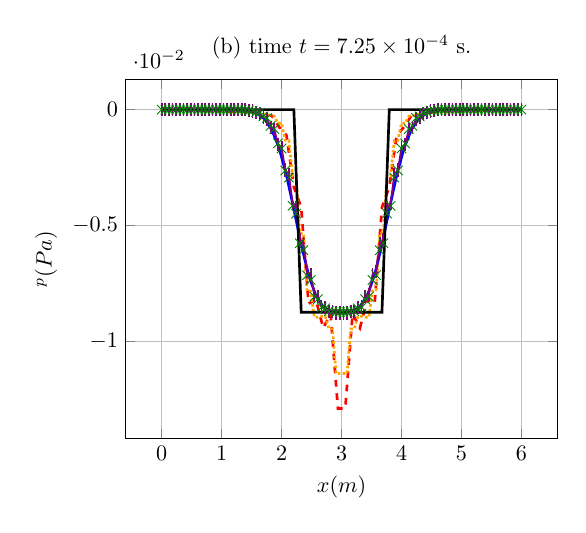
\begin{tikzpicture}[scale=0.8]
\begin{axis}[xlabel=$x (m)$,ylabel=$\eps^p (Pa)$,ymajorgrids=true,xmajorgrids=true,legend pos=outer north east,title={(b) time $t = 7.25\times 10^{-4} $ s.}]
\addplot[Red,very thick,mark=none,dashed,mark size=3pt] coordinates {(0.0,0.0) (0.12244897959183673,0.0) (0.24489795918367346,0.0) (0.36734693877551017,0.0) (0.4897959183673469,0.0) (0.6122448979591837,-3.577487902203997e-05) (0.7346938775510203,-6.306588245633642e-05) (0.8571428571428571,-6.949496312549484e-05) (0.9795918367346939,-8.005219978840035e-05) (1.1020408163265305,-9.009475914811774e-05) (1.2244897959183674,-9.858795071160678e-05) (1.346938775510204,-0.00010648019894997112) (1.4693877551020407,-0.00012616863649930955) (1.5918367346938775,-0.0001362011171739252) (1.7142857142857142,-0.00021257027814173217) (1.836734693877551,-0.00026486085096336456) (1.9591836734693877,-0.0007517028599145731) (2.0816326530612246,-0.0011133976998079925) (2.204081632653061,-0.003333993937447701) (2.326530612244898,-0.004209977621639336) (2.4489795918367347,-0.008357654568129739) (2.571428571428571,-0.00818541244484605) (2.693877551020408,-0.009408157524816411) (2.816326530612245,-0.008806354443804355) (2.9387755102040813,-0.012877303196726952) (3.061224489795918,-0.012877303196726607) (3.183673469387755,-0.008806354443804494) (3.306122448979592,-0.00940815752481628) (3.4285714285714284,-0.00818541244484614) (3.5510204081632653,-0.008357654568129634) (3.673469387755102,-0.004209977621639346) (3.7959183673469385,-0.0033339939374476507) (3.9183673469387754,-0.0011133976998079806) (4.040816326530612,-0.0007517028599145573) (4.163265306122449,-0.0002648608509633606) (4.285714285714286,-0.0002125702781417296) (4.408163265306122,-0.00013620111717393342) (4.530612244897959,-0.00012616863649931356) (4.653061224489796,-0.00010648019894998299) (4.775510204081632,-9.858795071160708e-05) (4.8979591836734695,-9.00947591481104e-05) (5.020408163265306,-8.005219978840008e-05) (5.142857142857142,-6.949496312550109e-05) (5.26530612244898,-6.306588245633955e-05) (5.387755102040816,-3.5774879022040825e-05) (5.5102040816326525,0.0) (5.63265306122449,0.0) (5.755102040816326,0.0) (5.877551020408163,0.0) (6.0,0.0) };
\addplot[Orange,very thick,mark=none,densely dotted,mark size=3pt] coordinates {(0.0,0.0) (0.06060606060606061,0.0) (0.12121212121212122,0.0) (0.18181818181818182,0.0) (0.24242424242424243,0.0) (0.30303030303030304,0.0) (0.36363636363636365,0.0) (0.42424242424242425,0.0) (0.48484848484848486,-1.3923950014088835e-06) (0.5454545454545454,-1.3923950014088835e-06) (0.6060606060606061,-4.802593874190819e-05) (0.6666666666666667,-4.802593874190819e-05) (0.7272727272727273,-6.41910410194221e-05) (0.7878787878787878,-6.41910410194221e-05) (0.8484848484848485,-6.859024545017706e-05) (0.9090909090909092,-6.859024545017706e-05) (0.9696969696969697,-7.288774581652991e-05) (1.0303030303030303,-7.288774581652991e-05) (1.0909090909090908,-8.507726423586093e-05) (1.1515151515151516,-8.507726423586093e-05) (1.2121212121212122,-9.691077127878779e-05) (1.2727272727272727,-9.691077127878779e-05) (1.3333333333333335,-0.0001071106301627928) (1.393939393939394,-0.0001071106301627928) (1.4545454545454546,-0.00011891582560129873) (1.5151515151515151,-0.00011891582560129873) (1.5757575757575757,-0.0001411626480808113) (1.6363636363636365,-0.0001411626480808113) (1.696969696969697,-0.00018474128224396107) (1.7575757575757576,-0.00018474128224396107) (1.8181818181818183,-0.00028928129016686006) (1.878787878787879,-0.00028928129016686006) (1.9393939393939394,-0.0005871331097401253) (2.0,-0.0005871331097401253) (2.0606060606060606,-0.0013271912464349832) (2.121212121212121,-0.0013271912464349832) (2.1818181818181817,-0.0028650643902802643) (2.2424242424242427,-0.0028650643902802643) (2.303030303030303,-0.005330257320518476) (2.3636363636363638,-0.005330257320518476) (2.4242424242424243,-0.007825827621282502) (2.484848484848485,-0.007825827621282502) (2.5454545454545454,-0.008947666418341944) (2.606060606060606,-0.008947666418341944) (2.666666666666667,-0.008904688564068288) (2.7272727272727275,-0.008904688564068288) (2.787878787878788,-0.00944634271615033) (2.8484848484848486,-0.00944634271615033) (2.909090909090909,-0.011373543353957122) (2.9696969696969697,-0.011373543353957122) (3.0303030303030303,-0.011373543353957112) (3.090909090909091,-0.011373543353957112) (3.1515151515151514,-0.009446342716150326) (3.2121212121212124,-0.009446342716150326) (3.272727272727273,-0.008904688564068298) (3.3333333333333335,-0.008904688564068298) (3.393939393939394,-0.008947666418341943) (3.4545454545454546,-0.008947666418341943) (3.515151515151515,-0.0078258276212825) (3.5757575757575757,-0.0078258276212825) (3.6363636363636367,-0.005330257320518468) (3.6969696969696972,-0.005330257320518468) (3.757575757575758,-0.002865064390280257) (3.8181818181818183,-0.002865064390280257) (3.878787878787879,-0.0013271912464349839) (3.9393939393939394,-0.0013271912464349839) (4.0,-0.0005871331097401301) (4.0606060606060606,-0.0005871331097401301) (4.121212121212121,-0.00028928129016686055) (4.181818181818182,-0.00028928129016686055) (4.242424242424242,-0.00018474128224395513) (4.303030303030303,-0.00018474128224395513) (4.363636363636363,-0.00014116264808081218) (4.424242424242425,-0.00014116264808081218) (4.484848484848485,-0.00011891582560129933) (4.545454545454546,-0.00011891582560129933) (4.606060606060606,-0.00010711063016279029) (4.666666666666667,-0.00010711063016279029) (4.7272727272727275,-9.691077127878893e-05) (4.787878787878788,-9.691077127878893e-05) (4.848484848484849,-8.507726423586494e-05) (4.909090909090909,-8.507726423586494e-05) (4.96969696969697,-7.288774581652709e-05) (5.03030303030303,-7.288774581652709e-05) (5.090909090909091,-6.859024545017819e-05) (5.151515151515151,-6.859024545017819e-05) (5.212121212121212,-6.419104101942352e-05) (5.2727272727272725,-6.419104101942352e-05) (5.333333333333334,-4.8025938741907344e-05) (5.3939393939393945,-4.8025938741907344e-05) (5.454545454545455,-1.3923950014085998e-06) (5.515151515151516,-1.3923950014085998e-06) (5.575757575757576,0.0) (5.636363636363637,0.0) (5.696969696969697,0.0) (5.757575757575758,0.0) (5.818181818181818,0.0) (5.878787878787879,0.0) (5.9393939393939394,0.0) (6.0,0.0) };
\addplot[Blue,very thick,mark=none,solid,mark size=3pt] coordinates {(0.0,-5.676632835751488e-19) (0.12244897959183673,-2.3898624238513766e-16) (0.24489795918367346,-3.735990751357306e-14) (0.36734693877551017,-2.3089144911084856e-12) (0.4897959183673469,-7.596762237094698e-11) (0.6122448979591837,-1.5415975357804979e-09) (0.7346938775510203,-1.0275730242331822e-08) (0.8571428571428571,-5.981932516353471e-08) (0.9795918367346939,-3.055798037968931e-07) (1.1020408163265305,-1.3747043608148892e-06) (1.2244897959183674,-5.4602719905226e-06) (1.346938775510204,-1.91823238251513e-05) (1.4693877551020407,-5.966726802674588e-05) (1.5918367346938775,-0.000164418651493838) (1.7142857142857142,-0.00040143744754996674) (1.836734693877551,-0.000868463225449077) (1.9591836734693877,-0.001665203797267752) (2.0816326530612246,-0.002832906100451628) (2.204081632653061,-0.004287995453610066) (2.326530612244898,-0.0058084443808726115) (2.4489795918367347,-0.007115753990208403) (2.571428571428571,-0.008016433919475449) (2.693877551020408,-0.008494471552590508) (2.816326530612245,-0.008677965053198252) (2.9387755102040813,-0.008723301560471332) (3.061224489795918,-0.008723301560471332) (3.183673469387755,-0.008677965053198252) (3.306122448979592,-0.00849447155259052) (3.4285714285714284,-0.008016433919475457) (3.5510204081632653,-0.007115753990208413) (3.673469387755102,-0.005808444380872623) (3.7959183673469385,-0.004287995453610076) (3.9183673469387754,-0.0028329061004516366) (4.040816326530612,-0.0016652037972677586) (4.163265306122449,-0.00086846322544908) (4.285714285714286,-0.0004014374475499613) (4.408163265306122,-0.00016441865149382611) (4.530612244897959,-5.9667268026732546e-05) (4.653061224489796,-1.918232382513086e-05) (4.775510204081632,-5.460271990507557e-06) (4.8979591836734695,-1.3747043608103478e-06) (5.020408163265306,-3.055798037929194e-07) (5.142857142857142,-5.981932515587126e-08) (5.26530612244898,-1.027573023324921e-08) (5.387755102040816,-1.5415975312391917e-09) (5.5102040816326525,-7.596762123562041e-11) (5.63265306122449,-2.308913923445202e-12) (5.755102040816326,-3.7358772187005907e-14) (5.877551020408163,-2.4097306387765065e-16) (6.0,-8.514949253627233e-19) };
\addplot[Purple,thick,mark=|,solid,mark size=3pt] coordinates {(0.0,0.0) (0.06060606060606061,0.0) (0.12121212121212122,0.0) (0.18181818181818182,0.0) (0.24242424242424243,0.0) (0.30303030303030304,0.0) (0.36363636363636365,0.0) (0.42424242424242425,0.0) (0.48484848484848486,0.0) (0.5454545454545454,0.0) (0.6060606060606061,0.0) (0.6666666666666667,0.0) (0.7272727272727273,0.0) (0.7878787878787878,0.0) (0.8484848484848485,0.0) (0.9090909090909092,0.0) (0.9696969696969697,0.0) (1.0303030303030303,0.0) (1.0909090909090908,0.0) (1.1515151515151516,-4.1375394533929374e-08) (1.2121212121212122,-1.6766275644359134e-07) (1.2727272727272727,-3.6899460485265364e-07) (1.3333333333333335,-3.7730684118324803e-06) (1.393939393939394,-6.566829345463855e-06) (1.4545454545454546,-3.9533489461271815e-05) (1.5151515151515151,-5.4725319017766484e-05) (1.5757575757575757,-0.0001393994522696901) (1.6363636363636365,-0.00016538778038305982) (1.696969696969697,-0.00034692599494932723) (1.7575757575757576,-0.0003991527105652267) (1.8181818181818183,-0.0007625905945333334) (1.878787878787879,-0.0008563059468014388) (1.9393939393939394,-0.0014922856868946723) (2.0,-0.0016374885246225213) (2.0606060606060606,-0.0025987877617010637) (2.121212121212121,-0.002790686204907401) (2.1818181818181817,-0.004030984098849627) (2.2424242424242427,-0.004243936219158137) (2.303030303030303,-0.0055885132243183545) (2.3636363636363638,-0.005782685656220611) (2.4242424242424243,-0.0069809715690837505) (2.484848484848485,-0.007121908461224029) (2.5454545454545454,-0.007972241161582445) (2.606060606060606,-0.008049596395188874) (2.666666666666667,-0.008505818537721688) (2.7272727272727275,-0.008534811001440776) (2.787878787878788,-0.008702033969468866) (2.8484848484848486,-0.008707545856799517) (2.909090909090909,-0.008758042662148493) (2.9696969696969697,-0.008762227333878615) (3.0303030303030303,-0.008762227333878615) (3.090909090909091,-0.008758042662148495) (3.1515151515151514,-0.008707545856799517) (3.2121212121212124,-0.008702033969468868) (3.272727272727273,-0.008534811001440776) (3.3333333333333335,-0.00850581853772169) (3.393939393939394,-0.008049596395188876) (3.4545454545454546,-0.007972241161582454) (3.515151515151515,-0.007121908461224033) (3.5757575757575757,-0.006980971569083754) (3.6363636363636367,-0.0057826856562206205) (3.6969696969696972,-0.005588513224318365) (3.757575757575758,-0.004243936219158141) (3.8181818181818183,-0.00403098409884963) (3.878787878787879,-0.0027906862049074093) (3.9393939393939394,-0.002598787761701072) (4.0,-0.0016374885246225263) (4.0606060606060606,-0.0014922856868946775) (4.121212121212121,-0.0008563059468014425) (4.181818181818182,-0.0007625905945333374) (4.242424242424242,-0.00039915271056523323) (4.303030303030303,-0.00034692599494933374) (4.363636363636363,-0.00016538778038306773) (4.424242424242425,-0.00013939945226969862) (4.484848484848485,-5.472531901777926e-05) (4.545454545454546,-3.9533489461283464e-05) (4.606060606060606,-6.566829345470383e-06) (4.666666666666667,-3.773068411838724e-06) (4.7272727272727275,-3.68994604853789e-07) (4.787878787878788,-1.6766275644359137e-07) (4.848484848484849,-4.1375394533929374e-08) (4.909090909090909,0.0) (4.96969696969697,0.0) (5.03030303030303,0.0) (5.090909090909091,0.0) (5.151515151515151,0.0) (5.212121212121212,0.0) (5.2727272727272725,0.0) (5.333333333333334,0.0) (5.3939393939393945,0.0) (5.454545454545455,0.0) (5.515151515151516,0.0) (5.575757575757576,0.0) (5.636363636363637,0.0) (5.696969696969697,0.0) (5.757575757575758,0.0) (5.818181818181818,0.0) (5.878787878787879,0.0) (5.9393939393939394,0.0) (6.0,0.0) };
\addplot[Green,thin,mark=x,only marks,mark size=3pt] coordinates {(0.0,-5.676632835751488e-19) (0.06060606060606061,0.0) (0.12121212121212122,-5.960464477539063e-18) (0.18181818181818182,-8.231117611839657e-18) (0.24242424242424243,-1.2593609946114675e-15) (0.30303030303030304,-2.566973368326823e-15) (0.36363636363636365,-1.2795357477097285e-13) (0.42424242424242425,-2.4569800921848845e-13) (0.48484848484848486,-6.614250512350173e-12) (0.5454545454545454,-1.1978970822833834e-11) (0.6060606060606061,-2.014539040270306e-10) (0.6666666666666667,-3.4473041437921067e-10) (0.7272727272727273,-1.7396754244963327e-09) (0.7878787878787878,-2.878236005703608e-09) (0.8484848484848485,-1.2915230488493328e-08) (0.9090909090909092,-2.0645992022468928e-08) (0.9696969696969697,-8.27788498841581e-08) (1.0303030303030303,-1.2777907757077899e-07) (1.0909090909090908,-4.594512838170642e-07) (1.1515151515151516,-6.844381126222156e-07) (1.2121212121212122,-2.2128580056431746e-06) (1.2727272727272727,-3.179616010181393e-06) (1.3333333333333335,-9.259748040896655e-06) (1.393939393939394,-1.2827869456145025e-05) (1.4545454545454546,-3.368426530185115e-05) (1.5151515151515151,-4.497549873773654e-05) (1.5757575757575757,-0.00010652981117383356) (1.6363636363636365,-0.0001370713310835756) (1.696969696969697,-0.00029284351963117065) (1.7575757575757576,-0.0003631417363302577) (1.8181818181818183,-0.0006995518818956783) (1.878787878787879,-0.0008364026933450982) (1.9393939393939394,-0.0014524891643318866) (2.0,-0.0016759867374438234) (2.0606060606060606,-0.002624841264006548) (2.121212121212121,-0.002927791589407064) (2.1818181818181817,-0.004143496150492473) (2.2424242424242427,-0.004479523423076173) (2.303030303030303,-0.00575685976116301) (2.3636363636363638,-0.006056043282157859) (2.4242424242424243,-0.007135597694533012) (2.484848484848485,-0.007343753961930436) (2.5454545454545454,-0.008058153161608643) (2.606060606060606,-0.008166928046930103) (2.666666666666667,-0.008522695893558911) (2.7272727272727275,-0.008562766723745093) (2.787878787878788,-0.008687900335388849) (2.8484848484848486,-0.008697160560944411) (2.909090909090909,-0.00872482225316362) (2.9696969696969697,-0.008725830219873004) (3.0303030303030303,-0.008725830219873004) (3.090909090909091,-0.00872482225316362) (3.1515151515151514,-0.008697160560944413) (3.2121212121212124,-0.008687900335388852) (3.272727272727273,-0.008562766723745095) (3.3333333333333335,-0.008522695893558915) (3.393939393939394,-0.008166928046930103) (3.4545454545454546,-0.008058153161608647) (3.515151515151515,-0.007343753961930437) (3.5757575757575757,-0.007135597694533014) (3.6363636363636367,-0.006056043282157861) (3.6969696969696972,-0.005756859761163013) (3.757575757575758,-0.004479523423076173) (3.8181818181818183,-0.004143496150492474) (3.878787878787879,-0.002927791589407064) (3.9393939393939394,-0.0026248412640065494) (4.0,-0.0016759867374438234) (4.0606060606060606,-0.0014524891643318892) (4.121212121212121,-0.0008364026933450992) (4.181818181818182,-0.0006995518818956805) (4.242424242424242,-0.00036314173633026085) (4.303030303030303,-0.0002928435196311738) (4.363636363636363,-0.00013707133108358015) (4.424242424242425,-0.00010652981117383724) (4.484848484848485,-4.497549873774307e-05) (4.545454545454546,-3.3684265301855976e-05) (4.606060606060606,-1.2827869456148999e-05) (4.666666666666667,-9.259748040899208e-06) (4.7272727272727275,-3.1796160101867863e-06) (4.787878787878788,-2.2128580056479997e-06) (4.848484848484849,-6.844381126324336e-07) (4.909090909090909,-4.5945128382728215e-07) (4.96969696969697,-1.277790775790101e-07) (5.03030303030303,-8.27788498932407e-08) (5.090909090909091,-2.0645992028145564e-08) (5.151515151515151,-1.2915230493318468e-08) (5.212121212121212,-2.878236009109588e-09) (5.2727272727272725,-1.7396754279023124e-09) (5.333333333333334,-3.4473041579836887e-10) (5.3939393939393945,-2.014539034593673e-10) (5.454545454545455,-1.1978968552180698e-11) (5.515151515151516,-6.614249377023606e-12) (5.575757575757576,-2.45694603238787e-13) (5.636363636363637,-1.2795045262291317e-13) (5.696969696969697,-2.566405705043248e-15) (5.757575757575758,-1.2633346375964938e-15) (5.818181818181818,-1.2772423880440849e-17) (5.878787878787879,-6.528127761114212e-18) (5.9393939393939394,0.0) (6.0,0.0) };
\addplot[black,very thick,mark=pentagone*,solid,mark size=3pt] coordinates {(0.0,-0.0) (0.12244897959183673,-0.0) (0.24489795918367346,-0.0) (0.36734693877551017,-0.0) (0.4897959183673469,-0.0) (0.6122448979591837,-0.0) (0.7346938775510203,-0.0) (0.8571428571428571,-0.0) (0.9795918367346939,-0.0) (1.1020408163265305,-0.0) (1.2244897959183674,-0.0) (1.346938775510204,-0.0) (1.4693877551020407,-0.0) (1.5918367346938775,-0.0) (1.7142857142857142,-0.0) (1.836734693877551,-0.0) (1.9591836734693877,-0.0) (2.0816326530612246,-0.0) (2.204081632653061,-0.0) (2.326530612244898,-0.008728715609439695) (2.4489795918367347,-0.008728715609439695) (2.571428571428571,-0.008728715609439695) (2.693877551020408,-0.008728715609439695) (2.816326530612245,-0.008728715609439695) (2.9387755102040813,-0.008728715609439695) (3.061224489795918,-0.008728715609439695) (3.183673469387755,-0.008728715609439695) (3.306122448979592,-0.008728715609439695) (3.4285714285714284,-0.008728715609439695) (3.5510204081632653,-0.008728715609439695) (3.673469387755102,-0.008728715609439695) (3.7959183673469385,-0.0) (3.9183673469387754,-0.0) (4.040816326530612,-0.0) (4.163265306122449,-0.0) (4.285714285714286,-0.0) (4.408163265306122,-0.0) (4.530612244897959,-0.0) (4.653061224489796,-0.0) (4.775510204081632,-0.0) (4.8979591836734695,-0.0) (5.020408163265306,-0.0) (5.142857142857142,-0.0) (5.26530612244898,-0.0) (5.387755102040816,-0.0) (5.5102040816326525,-0.0) (5.63265306122449,-0.0) (5.755102040816326,-0.0) (5.877551020408163,-0.0) (6.0,-0.0) };
%\legend{usl 1ppc,usl 2ppc,dgmpm 1ppc,dgmpm 2ppc,dgmpm 2ppc (RK2),exact}
\end{axis}
\end{tikzpicture}
%%% Local Variables:
%%% mode: latex
%%% TeX-master: "../../mainManuscript"
%%% End:
}
%   {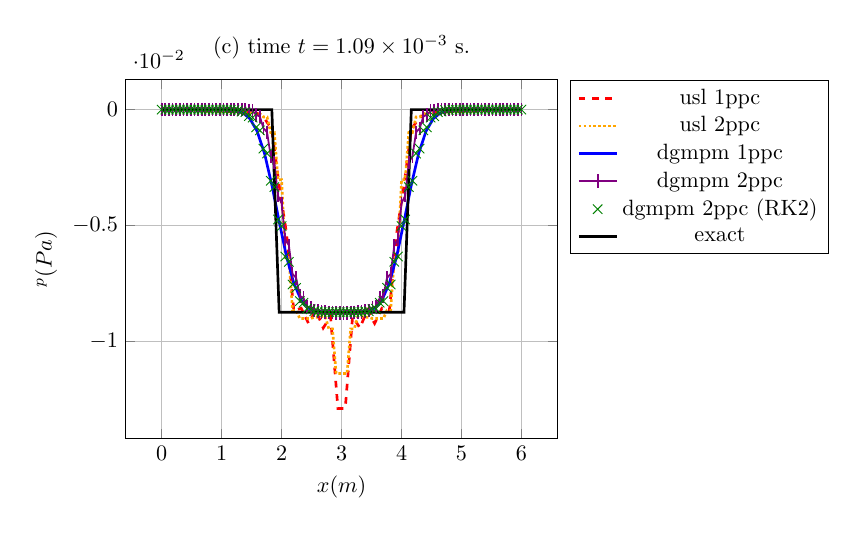
\begin{tikzpicture}[scale=0.8]
\begin{axis}[xlabel=$x (m)$,ylabel=$\eps^p (Pa)$,ymajorgrids=true,xmajorgrids=true,legend pos=outer north east,title={(c) time $t = 1.09\times 10^{-3} $ s.}]
\addplot[Red,very thick,mark=none,dashed,mark size=3pt] coordinates {(0.0,0.0) (0.12244897959183673,0.0) (0.24489795918367346,0.0) (0.36734693877551017,0.0) (0.4897959183673469,0.0) (0.6122448979591837,-3.577487902203997e-05) (0.7346938775510203,-6.306588245633642e-05) (0.8571428571428571,-6.949496312549484e-05) (0.9795918367346939,-8.005219978840035e-05) (1.1020408163265305,-9.009475914811774e-05) (1.2244897959183674,-9.858795071160678e-05) (1.346938775510204,-0.00010648019894997112) (1.4693877551020407,-0.00013090237763271645) (1.5918367346938775,-0.00015585484694440393) (1.7142857142857142,-0.00037807434010367157) (1.836734693877551,-0.0008542508721889013) (1.9591836734693877,-0.003265580636192999) (2.0816326530612246,-0.005332403663610279) (2.204081632653061,-0.008685547798871193) (2.326530612244898,-0.008557827562005196) (2.4489795918367347,-0.009212270529983918) (2.571428571428571,-0.008640321746270047) (2.693877551020408,-0.009408157524816411) (2.816326530612245,-0.008914806029937274) (2.9387755102040813,-0.012877303196726952) (3.061224489795918,-0.012877303196726607) (3.183673469387755,-0.008914806029937388) (3.306122448979592,-0.00940815752481628) (3.4285714285714284,-0.008640321746270135) (3.5510204081632653,-0.009212270529983827) (3.673469387755102,-0.008557827562005267) (3.7959183673469385,-0.008685547798871113) (3.9183673469387754,-0.005332403663610266) (4.040816326530612,-0.003265580636192934) (4.163265306122449,-0.0008542508721888987) (4.285714285714286,-0.00037807434010366447) (4.408163265306122,-0.00015585484694441217) (4.530612244897959,-0.00013090237763272187) (4.653061224489796,-0.00010648019894998299) (4.775510204081632,-9.858795071160708e-05) (4.8979591836734695,-9.00947591481104e-05) (5.020408163265306,-8.005219978840008e-05) (5.142857142857142,-6.949496312550109e-05) (5.26530612244898,-6.306588245633955e-05) (5.387755102040816,-3.5774879022040825e-05) (5.5102040816326525,0.0) (5.63265306122449,0.0) (5.755102040816326,0.0) (5.877551020408163,0.0) (6.0,0.0) };
\addplot[Orange,very thick,mark=none,densely dotted,mark size=3pt] coordinates {(0.0,0.0) (0.06060606060606061,0.0) (0.12121212121212122,0.0) (0.18181818181818182,0.0) (0.24242424242424243,0.0) (0.30303030303030304,0.0) (0.36363636363636365,0.0) (0.42424242424242425,0.0) (0.48484848484848486,-1.3923950014088835e-06) (0.5454545454545454,-1.3923950014088835e-06) (0.6060606060606061,-4.802593874190819e-05) (0.6666666666666667,-4.802593874190819e-05) (0.7272727272727273,-6.41910410194221e-05) (0.7878787878787878,-6.41910410194221e-05) (0.8484848484848485,-6.859024545017706e-05) (0.9090909090909092,-6.859024545017706e-05) (0.9696969696969697,-7.288774581652991e-05) (1.0303030303030303,-7.288774581652991e-05) (1.0909090909090908,-8.507726423586093e-05) (1.1515151515151516,-8.507726423586093e-05) (1.2121212121212122,-9.691077127878779e-05) (1.2727272727272727,-9.691077127878779e-05) (1.3333333333333335,-0.00010711649363712468) (1.393939393939394,-0.00010711649363712468) (1.4545454545454546,-0.00012487268940087668) (1.5151515151515151,-0.00012487268940087668) (1.5757575757575757,-0.00016846150368530778) (1.6363636363636365,-0.00016846150368530778) (1.696969696969697,-0.00032141238951341054) (1.7575757575757576,-0.00032141238951341054) (1.8181818181818183,-0.0009863835722303473) (1.878787878787879,-0.0009863835722303473) (1.9393939393939394,-0.003025063907376677) (2.0,-0.003025063907376677) (2.0606060606060606,-0.006366348809033719) (2.121212121212121,-0.006366348809033719) (2.1818181818181817,-0.008647239978151484) (2.2424242424242427,-0.008647239978151484) (2.303030303030303,-0.009001860585213824) (2.3636363636363638,-0.009001860585213824) (2.4242424242424243,-0.009001507335175213) (2.484848484848485,-0.009001507335175213) (2.5454545454545454,-0.008949274888554966) (2.606060606060606,-0.008949274888554966) (2.666666666666667,-0.00891581762874243) (2.7272727272727275,-0.00891581762874243) (2.787878787878788,-0.00944634271615033) (2.8484848484848486,-0.00944634271615033) (2.909090909090909,-0.011373543353957122) (2.9696969696969697,-0.011373543353957122) (3.0303030303030303,-0.011373543353957112) (3.090909090909091,-0.011373543353957112) (3.1515151515151514,-0.009446342716150326) (3.2121212121212124,-0.009446342716150326) (3.272727272727273,-0.00891581762874244) (3.3333333333333335,-0.00891581762874244) (3.393939393939394,-0.008949274888554966) (3.4545454545454546,-0.008949274888554966) (3.515151515151515,-0.009001507335175215) (3.5757575757575757,-0.009001507335175215) (3.6363636363636367,-0.009001860585213826) (3.6969696969696972,-0.009001860585213826) (3.757575757575758,-0.008647239978151493) (3.8181818181818183,-0.008647239978151493) (3.878787878787879,-0.006366348809033716) (3.9393939393939394,-0.006366348809033716) (4.0,-0.003025063907376669) (4.0606060606060606,-0.003025063907376669) (4.121212121212121,-0.0009863835722303564) (4.181818181818182,-0.0009863835722303564) (4.242424242424242,-0.00032141238951339976) (4.303030303030303,-0.00032141238951339976) (4.363636363636363,-0.00016846150368530894) (4.424242424242425,-0.00016846150368530894) (4.484848484848485,-0.00012487268940087758) (4.545454545454546,-0.00012487268940087758) (4.606060606060606,-0.00010711649363712272) (4.666666666666667,-0.00010711649363712272) (4.7272727272727275,-9.691077127878893e-05) (4.787878787878788,-9.691077127878893e-05) (4.848484848484849,-8.507726423586494e-05) (4.909090909090909,-8.507726423586494e-05) (4.96969696969697,-7.288774581652709e-05) (5.03030303030303,-7.288774581652709e-05) (5.090909090909091,-6.859024545017819e-05) (5.151515151515151,-6.859024545017819e-05) (5.212121212121212,-6.419104101942352e-05) (5.2727272727272725,-6.419104101942352e-05) (5.333333333333334,-4.8025938741907344e-05) (5.3939393939393945,-4.8025938741907344e-05) (5.454545454545455,-1.3923950014085998e-06) (5.515151515151516,-1.3923950014085998e-06) (5.575757575757576,0.0) (5.636363636363637,0.0) (5.696969696969697,0.0) (5.757575757575758,0.0) (5.818181818181818,0.0) (5.878787878787879,0.0) (5.9393939393939394,0.0) (6.0,0.0) };
\addplot[Blue,very thick,mark=none,solid,mark size=3pt] coordinates {(0.0,-5.676632835751488e-19) (0.12244897959183673,-2.3898624238513766e-16) (0.24489795918367346,-3.735990751357306e-14) (0.36734693877551017,-2.3089144911084856e-12) (0.4897959183673469,-7.596762237094698e-11) (0.6122448979591837,-1.5415975357804979e-09) (0.7346938775510203,-2.1087029002110162e-08) (0.8571428571428571,-2.0628580472526095e-07) (0.9795918367346939,-1.5051975779320511e-06) (1.1020408163265305,-8.452232526292688e-06) (1.2244897959183674,-3.741900938747327e-05) (1.346938775510204,-0.00013315210803806102) (1.4693877551020407,-0.00038701776930482674) (1.5918367346938775,-0.0009319386970470464) (1.7142857142857142,-0.0018842066770200564) (1.836734693877551,-0.0032431409441831516) (1.9591836734693877,-0.004827293901207316) (2.0816326530612246,-0.00633202118341673) (2.204081632653061,-0.007489880430691718) (2.326530612244898,-0.008204526972019307) (2.4489795918367347,-0.008552921390073501) (2.571428571428571,-0.008674876019514461) (2.693877551020408,-0.008716486656783273) (2.816326530612245,-0.008726887116624966) (2.9387755102040813,-0.008728580772745199) (3.061224489795918,-0.008728580772745199) (3.183673469387755,-0.008726887116624966) (3.306122448979592,-0.00871648665678328) (3.4285714285714284,-0.008674876019514466) (3.5510204081632653,-0.008552921390073511) (3.673469387755102,-0.008204526972019318) (3.7959183673469385,-0.007489880430691721) (3.9183673469387754,-0.00633202118341673) (4.040816326530612,-0.0048272939012073204) (4.163265306122449,-0.0032431409441831525) (4.285714285714286,-0.001884206677020053) (4.408163265306122,-0.0009319386970470392) (4.530612244897959,-0.0003870177693048181) (4.653061224489796,-0.0001331521080380519) (4.775510204081632,-3.7419009387462476e-05) (4.8979591836734695,-8.452232526284741e-06) (5.020408163265306,-1.5051975779246716e-06) (5.142857142857142,-2.0628580471617835e-07) (5.26530612244898,-2.1087028991608393e-08) (5.387755102040816,-1.5415975312391917e-09) (5.5102040816326525,-7.596762123562041e-11) (5.63265306122449,-2.308913923445202e-12) (5.755102040816326,-3.7358772187005907e-14) (5.877551020408163,-2.4097306387765065e-16) (6.0,-8.514949253627233e-19) };
\addplot[Purple,thick,mark=|,solid,mark size=3pt] coordinates {(0.0,0.0) (0.06060606060606061,0.0) (0.12121212121212122,0.0) (0.18181818181818182,0.0) (0.24242424242424243,0.0) (0.30303030303030304,0.0) (0.36363636363636365,0.0) (0.42424242424242425,0.0) (0.48484848484848486,0.0) (0.5454545454545454,0.0) (0.6060606060606061,0.0) (0.6666666666666667,0.0) (0.7272727272727273,0.0) (0.7878787878787878,0.0) (0.8484848484848485,0.0) (0.9090909090909092,0.0) (0.9696969696969697,0.0) (1.0303030303030303,0.0) (1.0909090909090908,0.0) (1.1515151515151516,-4.1375394533929374e-08) (1.2121212121212122,-1.6766275644359134e-07) (1.2727272727272727,-3.6899460485265364e-07) (1.3333333333333335,-3.7730684118324803e-06) (1.393939393939394,-6.566829345463855e-06) (1.4545454545454546,-3.9533489461271815e-05) (1.5151515151515151,-5.787873091723124e-05) (1.5757575757575757,-0.0002274525995650831) (1.6363636363636365,-0.00029636567097843057) (1.696969696969697,-0.0008043486101741406) (1.7575757575757576,-0.0009756904136278646) (1.8181818181818183,-0.002007506978689405) (1.878787878787879,-0.0022778320644552875) (1.9393939393939394,-0.0037101075201987303) (2.0,-0.004034858131037031) (2.0606060606060606,-0.005583330117719787) (2.121212121212121,-0.005852176347303774) (2.1818181818181817,-0.007081628136433296) (2.2424242424242427,-0.007249585758095964) (2.303030303030303,-0.008025296353006806) (2.3636363636363638,-0.008110184081085586) (2.4242424242424243,-0.008492622343293309) (2.484848484848485,-0.008525512701242518) (2.5454545454545454,-0.008671015536515168) (2.606060606060606,-0.008680086368368912) (2.666666666666667,-0.008720691408181637) (2.7272727272727275,-0.008722186625565662) (2.787878787878788,-0.00872959098319658) (2.8484848484848486,-0.008729715721981647) (2.909090909090909,-0.008758042662148493) (2.9696969696969697,-0.008762227333878615) (3.0303030303030303,-0.008762227333878615) (3.090909090909091,-0.008758042662148495) (3.1515151515151514,-0.008729715721981645) (3.2121212121212124,-0.008729590983196582) (3.272727272727273,-0.008722186625565662) (3.3333333333333335,-0.008720691408181639) (3.393939393939394,-0.00868008636836891) (3.4545454545454546,-0.008671015536515165) (3.515151515151515,-0.008525512701242514) (3.5757575757575757,-0.008492622343293309) (3.6363636363636367,-0.00811018408108559) (3.6969696969696972,-0.008025296353006812) (3.757575757575758,-0.007249585758095969) (3.8181818181818183,-0.0070816281364333026) (3.878787878787879,-0.005852176347303775) (3.9393939393939394,-0.005583330117719789) (4.0,-0.0040348581310370385) (4.0606060606060606,-0.0037101075201987394) (4.121212121212121,-0.0022778320644552983) (4.181818181818182,-0.002007506978689416) (4.242424242424242,-0.0009756904136278739) (4.303030303030303,-0.0008043486101741499) (4.363636363636363,-0.00029636567097843854) (4.424242424242425,-0.00022745259956509018) (4.484848484848485,-5.787873091724344e-05) (4.545454545454546,-3.9533489461283464e-05) (4.606060606060606,-6.566829345470383e-06) (4.666666666666667,-3.773068411838724e-06) (4.7272727272727275,-3.68994604853789e-07) (4.787878787878788,-1.6766275644359137e-07) (4.848484848484849,-4.1375394533929374e-08) (4.909090909090909,0.0) (4.96969696969697,0.0) (5.03030303030303,0.0) (5.090909090909091,0.0) (5.151515151515151,0.0) (5.212121212121212,0.0) (5.2727272727272725,0.0) (5.333333333333334,0.0) (5.3939393939393945,0.0) (5.454545454545455,0.0) (5.515151515151516,0.0) (5.575757575757576,0.0) (5.636363636363637,0.0) (5.696969696969697,0.0) (5.757575757575758,0.0) (5.818181818181818,0.0) (5.878787878787879,0.0) (5.9393939393939394,0.0) (6.0,0.0) };
\addplot[Green,thin,mark=x,only marks,mark size=3pt] coordinates {(0.0,-5.676632835751488e-19) (0.06060606060606061,0.0) (0.12121212121212122,-5.960464477539063e-18) (0.18181818181818182,-8.231117611839657e-18) (0.24242424242424243,-1.2593609946114675e-15) (0.30303030303030304,-2.566973368326823e-15) (0.36363636363636365,-1.2795357477097285e-13) (0.42424242424242425,-2.4569800921848845e-13) (0.48484848484848486,-6.614250512350173e-12) (0.5454545454545454,-1.1978970822833834e-11) (0.6060606060606061,-2.014539040270306e-10) (0.6666666666666667,-3.4473041437921067e-10) (0.7272727272727273,-3.958928195919309e-09) (0.7878787878787878,-6.412620588143667e-09) (0.8484848484848485,-5.3364499986455554e-08) (0.9090909090909092,-8.197237874269486e-08) (0.9696969696969697,-5.155914888793514e-07) (1.0303030303030303,-7.524956608332339e-07) (1.0909090909090908,-3.6911086009462675e-06) (1.1515151515151516,-5.128586973845675e-06) (1.2121212121212122,-2.0096823934549662e-05) (1.2727272727272727,-2.6639006500208663e-05) (1.3333333333333335,-8.500574414884647e-05) (1.393939393939394,-0.00010773647495164076) (1.4545454545454546,-0.00028442785366869175) (1.5151515151515151,-0.0003455251868600774) (1.5757575757575757,-0.0007651640013258602) (1.6363636363636365,-0.0008934272034897002) (1.696969696969697,-0.0016811593270009762) (1.7575757575757576,-0.001892798143971582) (1.8181818181818183,-0.0030669939640570066) (1.878787878787879,-0.0033423564247713746) (1.9393939393939394,-0.004734809703010922) (2.0,-0.005017334536365495) (2.0606060606060606,-0.006329679309076545) (2.121212121212121,-0.006557472732041174) (2.1818181818181817,-0.007536143497329047) (2.2424242424242427,-0.007679356454328646) (2.303030303030303,-0.00825193835878759) (2.3636363636363638,-0.008321206280476908) (2.4242424242424243,-0.008580337649446788) (2.484848484848485,-0.008605558443364046) (2.5454545454545454,-0.008686715531944143) (2.606060606060606,-0.008694798692719908) (2.666666666666667,-0.008720028673057422) (2.7272727272727275,-0.008721895117205144) (2.787878787878788,-0.008727550668862797) (2.8484848484848486,-0.008727826804119215) (2.909090909090909,-0.00872863974231939) (2.9696969696969697,-0.008728659383864157) (3.0303030303030303,-0.008728659383864159) (3.090909090909091,-0.008728639742319392) (3.1515151515151514,-0.008727826804119217) (3.2121212121212124,-0.008727550668862803) (3.272727272727273,-0.008721895117205145) (3.3333333333333335,-0.008720028673057423) (3.393939393939394,-0.008694798692719906) (3.4545454545454546,-0.008686715531944143) (3.515151515151515,-0.008605558443364044) (3.5757575757575757,-0.008580337649446788) (3.6363636363636367,-0.008321206280476912) (3.6969696969696972,-0.008251938358787594) (3.757575757575758,-0.007679356454328649) (3.8181818181818183,-0.0075361434973290516) (3.878787878787879,-0.006557472732041174) (3.9393939393939394,-0.006329679309076547) (4.0,-0.005017334536365494) (4.0606060606060606,-0.004734809703010924) (4.121212121212121,-0.0033423564247713777) (4.181818181818182,-0.0030669939640570088) (4.242424242424242,-0.0018927981439715827) (4.303030303030303,-0.001681159327000978) (4.363636363636363,-0.0008934272034897071) (4.424242424242425,-0.0007651640013258641) (4.484848484848485,-0.00034552518686008227) (4.545454545454546,-0.00028442785366869516) (4.606060606060606,-0.00010773647495164786) (4.666666666666667,-8.500574414885329e-05) (4.7272727272727275,-2.6639006500214904e-05) (4.787878787878788,-2.009682393455562e-05) (4.848484848484849,-5.1285869738558925e-06) (4.909090909090909,-3.6911086009562015e-06) (4.96969696969697,-7.524956608437356e-07) (5.03030303030303,-5.155914888895694e-07) (5.090909090909091,-8.197237874439784e-08) (5.151515151515151,-5.336449998730705e-08) (5.212121212121212,-6.412620592684973e-09) (5.2727272727272725,-3.958928200460616e-09) (5.333333333333334,-3.4473041579836887e-10) (5.3939393939393945,-2.014539034593673e-10) (5.454545454545455,-1.1978968552180698e-11) (5.515151515151516,-6.614249377023606e-12) (5.575757575757576,-2.45694603238787e-13) (5.636363636363637,-1.2795045262291317e-13) (5.696969696969697,-2.566405705043248e-15) (5.757575757575758,-1.2633346375964938e-15) (5.818181818181818,-1.2772423880440849e-17) (5.878787878787879,-6.528127761114212e-18) (5.9393939393939394,0.0) (6.0,0.0) };
\addplot[black,very thick,mark=pentagone*,solid,mark size=3pt] coordinates {(0.0,-0.0) (0.12244897959183673,-0.0) (0.24489795918367346,-0.0) (0.36734693877551017,-0.0) (0.4897959183673469,-0.0) (0.6122448979591837,-0.0) (0.7346938775510203,-0.0) (0.8571428571428571,-0.0) (0.9795918367346939,-0.0) (1.1020408163265305,-0.0) (1.2244897959183674,-0.0) (1.346938775510204,-0.0) (1.4693877551020407,-0.0) (1.5918367346938775,-0.0) (1.7142857142857142,-0.0) (1.836734693877551,-0.0) (1.9591836734693877,-0.008728715609439695) (2.0816326530612246,-0.008728715609439695) (2.204081632653061,-0.008728715609439695) (2.326530612244898,-0.008728715609439695) (2.4489795918367347,-0.008728715609439695) (2.571428571428571,-0.008728715609439695) (2.693877551020408,-0.008728715609439695) (2.816326530612245,-0.008728715609439695) (2.9387755102040813,-0.008728715609439695) (3.061224489795918,-0.008728715609439695) (3.183673469387755,-0.008728715609439695) (3.306122448979592,-0.008728715609439695) (3.4285714285714284,-0.008728715609439695) (3.5510204081632653,-0.008728715609439695) (3.673469387755102,-0.008728715609439695) (3.7959183673469385,-0.008728715609439695) (3.9183673469387754,-0.008728715609439695) (4.040816326530612,-0.008728715609439695) (4.163265306122449,-0.0) (4.285714285714286,-0.0) (4.408163265306122,-0.0) (4.530612244897959,-0.0) (4.653061224489796,-0.0) (4.775510204081632,-0.0) (4.8979591836734695,-0.0) (5.020408163265306,-0.0) (5.142857142857142,-0.0) (5.26530612244898,-0.0) (5.387755102040816,-0.0) (5.5102040816326525,-0.0) (5.63265306122449,-0.0) (5.755102040816326,-0.0) (5.877551020408163,-0.0) (6.0,-0.0) };
\legend{usl 1ppc,usl 2ppc,dgmpm 1ppc,dgmpm 2ppc,dgmpm 2ppc (RK2),exact}
\end{axis}
\end{tikzpicture}
%%% Local Variables:
%%% mode: latex
%%% TeX-master: "../../mainManuscript"
%%% End:
}
%   \caption{elastic-plastic RP epsp}
%   \label{fig:epsp_elastoplastic_RP}
% \end{figure}


Comparison with fvm and FEM (lumped mass matrix + radial return for integrating constitutive equations)
\begin{figure}[h!]
  \centering
  % {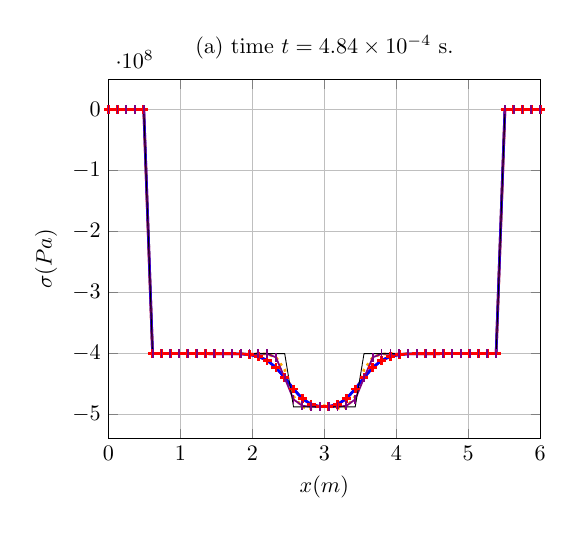
\begin{tikzpicture}[scale=0.8]
\begin{axis}[xlabel=$x (m)$,ylabel=$\sigma (Pa)$,ymajorgrids=true,xmajorgrids=true,legend pos=outer north east,title={(a) time $t = 4.84\times 10^{-4} $ s.},xmin=0.,xmax=6.]
\addplot[Red,very thick,mark=+,solid] coordinates {(0.0,-1.4032094709741823e-07) (0.12244897959183673,1.4032094709741797e-07) (0.24489795918367346,-5.501313561848306e-23) (0.36734693877551017,-1.4032094709741882e-07) (0.4897959183673469,-4.2096284129225576e-07) (0.6122448979591837,-400000000.0000052) (0.7346938775510203,-400000000.0003803) (0.8571428571428571,-400000000.0131417) (0.9795918367346939,-400000000.2874559) (1.1020408163265305,-400000004.46415013) (1.2244897959183674,-400000052.34678423) (1.346938775510204,-400000481.2046858) (1.4693877551020407,-400003554.03647596) (1.5918367346938775,-400021443.0967657) (1.7142857142857142,-400106894.9802318) (1.836734693877551,-400443646.6051052) (1.9591836734693877,-401540408.59283984) (2.0816326530612246,-404487333.2231472) (2.204081632653061,-410984305.87262785) (2.326530612244898,-422622254.02503896) (2.4489795918367347,-439299786.1010327) (2.571428571428571,-457971198.93456453) (2.693877551020408,-473710434.18348145) (2.816326530612245,-483108267.7934754) (2.9387755102040813,-486652315.1909913) (3.061224489795918,-486652315.1909913) (3.183673469387755,-483108267.7934754) (3.306122448979592,-473710434.18348145) (3.4285714285714284,-457971198.93456453) (3.5510204081632653,-439299786.1010328) (3.673469387755102,-422622254.025039) (3.7959183673469385,-410984305.8726279) (3.9183673469387754,-404487333.2231472) (4.040816326530612,-401540408.59283984) (4.163265306122449,-400443646.6051051) (4.285714285714286,-400106894.98023176) (4.408163265306122,-400021443.0967656) (4.530612244897959,-400003554.0364758) (4.653061224489796,-400000481.20468575) (4.775510204081632,-400000052.3467841) (4.8979591836734695,-400000004.46415013) (5.020408163265306,-400000000.2874559) (5.142857142857142,-400000000.01314175) (5.26530612244898,-400000000.0003803) (5.387755102040816,-400000000.0000052) (5.5102040816326525,1.403209470974181e-07) (5.63265306122449,-4.209628412922546e-07) (5.755102040816326,-7.335084749131074e-23) (5.877551020408163,-7.335084749131074e-23) (6.0,1.4032094709741816e-07) };
\addplot[Orange,very thick,mark=none,dotted] coordinates {(0.0011999999999999927,0.0) (0.12359999999999997,0.0) (0.24599999999999994,0.0) (0.36839999999999995,0.0) (0.4907999999999999,0.0) (0.6131999999999999,-399999999.9999996) (0.7355999999999999,-399999999.9999968) (0.858,-400000000.0) (0.9803999999999998,-399999999.9999996) (1.1027999999999998,-400000000.00000036) (1.2251999999999996,-400000000.0000013) (1.3475999999999997,-400000000.0000979) (1.4699999999999998,-400000000.00582314) (1.5923999999999996,-400000000.2649425) (1.7147999999999997,-400000009.2416795) (1.8371999999999995,-400000245.9026529) (1.9595999999999996,-400004932.9535555) (2.0819999999999994,-400073165.4563783) (2.2043999999999997,-400778734.27312934) (2.3267999999999995,-405684157.67745835) (2.4491999999999994,-426483554.2497189) (2.5715999999999997,-469882444.732417) (2.6939999999999995,-487460509.8573178) (2.8163999999999993,-489834934.6920107) (2.9387999999999996,-485390329.82597953) (3.0611999999999995,-485390329.8259847) (3.1835999999999993,-489834934.692009) (3.305999999999999,-487460509.85731673) (3.4283999999999994,-469882444.73241717) (3.5507999999999993,-426483554.2497191) (3.673199999999999,-405684157.67745817) (3.7955999999999994,-400778734.27312946) (3.9179999999999993,-400073165.4563784) (4.040399999999999,-400004932.95355564) (4.1628,-400000245.9026529) (4.2852,-400000009.2416795) (4.4076,-400000000.2649422) (4.53,-400000000.00582296) (4.6524,-400000000.0000977) (4.7748,-400000000.0000014) (4.8972,-400000000.00000036) (5.0196,-399999999.9999973) (5.142,-400000000.0) (5.2644,-400000000.0) (5.3868,-399999999.9999975) (5.5092,0.0) (5.6316,0.0) (5.754,0.0) (5.8764,0.0) (5.9988,0.0) };
\addplot[Blue,very thick,mark=none,solid] coordinates {(0.0011999999999999927,0.0) (0.12359999999999997,0.0) (0.24599999999999994,0.0) (0.36839999999999995,0.0) (0.4907999999999999,0.0) (0.6131999999999999,-400000000.0000052) (0.7355999999999999,-400000000.0003801) (0.858,-400000000.01314163) (0.9803999999999998,-400000000.2874559) (1.1027999999999998,-400000004.46415013) (1.2251999999999996,-400000052.3467841) (1.3475999999999997,-400000481.20468575) (1.4699999999999998,-400003554.03647584) (1.5923999999999996,-400021443.0967656) (1.7147999999999997,-400106894.9802317) (1.8371999999999995,-400443646.6051051) (1.9595999999999996,-401540408.5928399) (2.0819999999999994,-404487333.2231473) (2.2043999999999997,-410984305.8726279) (2.3267999999999995,-422622254.0250391) (2.4491999999999994,-439299786.10103285) (2.5715999999999997,-457971198.9345646) (2.6939999999999995,-473710434.1834816) (2.8163999999999993,-483108267.79347533) (2.9387999999999996,-486652315.1909914) (3.0611999999999995,-486652315.1909914) (3.1835999999999993,-483108267.79347533) (3.305999999999999,-473710434.1834816) (3.4283999999999994,-457971198.9345646) (3.5507999999999993,-439299786.10103285) (3.673199999999999,-422622254.0250391) (3.7955999999999994,-410984305.8726279) (3.9179999999999993,-404487333.2231473) (4.040399999999999,-401540408.5928399) (4.1628,-400443646.6051051) (4.2852,-400106894.9802317) (4.4076,-400021443.0967656) (4.53,-400003554.03647584) (4.6524,-400000481.20468575) (4.7748,-400000052.3467841) (4.8972,-400000004.46415013) (5.0196,-400000000.2874559) (5.142,-400000000.01314163) (5.2644,-400000000.0003801) (5.3868,-400000000.0000052) (5.5092,0.0) (5.6316,0.0) (5.754,0.0) (5.8764,0.0) (5.9988,0.0) };
\addplot[Purple,thick,mark=|,solid] coordinates {(0.0011999999999999927,0.0) (0.12359999999999997,0.0) (0.24599999999999994,0.0) (0.36839999999999995,0.0) (0.4907999999999999,0.0) (0.6131999999999999,-399999999.99999994) (0.7355999999999999,-400000000.0) (0.858,-400000000.0) (0.9803999999999998,-400000000.0) (1.1027999999999998,-400000000.0) (1.2251999999999996,-400000000.00000024) (1.3475999999999997,-400000000.00001407) (1.4699999999999998,-400000000.0007095) (1.5923999999999996,-400000000.0295273) (1.7147999999999997,-400000001.0283913) (1.8371999999999995,-400000030.33246076) (1.9595999999999996,-400000768.4378232) (2.0819999999999994,-400016975.1308303) (2.2043999999999997,-400318783.1149349) (2.3267999999999995,-405939608.94153374) (2.4491999999999994,-439871901.51192373) (2.5715999999999997,-475012040.0305417) (2.6939999999999995,-485411927.60231024) (2.8163999999999993,-487101987.7579666) (2.9387999999999996,-487278357.03341293) (3.0611999999999995,-487278357.03341293) (3.1835999999999993,-487101987.7579666) (3.305999999999999,-485411927.60231024) (3.4283999999999994,-475012040.0305417) (3.5507999999999993,-439871901.51192373) (3.673199999999999,-405939608.94153374) (3.7955999999999994,-400318783.1149349) (3.9179999999999993,-400016975.1308303) (4.040399999999999,-400000768.4378232) (4.1628,-400000030.33246076) (4.2852,-400000001.0283913) (4.4076,-400000000.0295273) (4.53,-400000000.0007095) (4.6524,-400000000.00001407) (4.7748,-400000000.0000003) (4.8972,-400000000.0) (5.0196,-400000000.0) (5.142,-400000000.0) (5.2644,-400000000.0) (5.3868,-399999999.99999994) (5.5092,0.0) (5.6316,0.0) (5.754,0.0) (5.8764,0.0) (5.9988,0.0) };
\addplot[black,thin,mark=none,solid] coordinates {(0.0,-0.0) (0.12244897959183673,-0.0) (0.24489795918367346,-0.0) (0.36734693877551017,-0.0) (0.4897959183673469,-0.0) (0.6122448979591837,-400000000.0) (0.7346938775510203,-400000000.0) (0.8571428571428571,-400000000.0) (0.9795918367346939,-400000000.0) (1.1020408163265305,-400000000.0) (1.2244897959183674,-400000000.0) (1.346938775510204,-400000000.0) (1.4693877551020407,-400000000.0) (1.5918367346938775,-400000000.0) (1.7142857142857142,-400000000.0) (1.836734693877551,-400000000.0) (1.9591836734693877,-400000000.0) (2.0816326530612246,-400000000.0) (2.204081632653061,-400000000.0) (2.326530612244898,-400000000.0) (2.4489795918367347,-400000000.0) (2.571428571428571,-487287156.09439695) (2.693877551020408,-487287156.09439695) (2.816326530612245,-487287156.09439695) (2.9387755102040813,-487287156.09439695) (3.061224489795918,-487287156.09439695) (3.183673469387755,-487287156.09439695) (3.306122448979592,-487287156.09439695) (3.4285714285714284,-487287156.09439695) (3.5510204081632653,-400000000.0) (3.673469387755102,-400000000.0) (3.7959183673469385,-400000000.0) (3.9183673469387754,-400000000.0) (4.040816326530612,-400000000.0) (4.163265306122449,-400000000.0) (4.285714285714286,-400000000.0) (4.408163265306122,-400000000.0) (4.530612244897959,-400000000.0) (4.653061224489796,-400000000.0) (4.775510204081632,-400000000.0) (4.8979591836734695,-400000000.0) (5.020408163265306,-400000000.0) (5.142857142857142,-400000000.0) (5.26530612244898,-400000000.0) (5.387755102040816,-400000000.0) (5.5102040816326525,-0.0) (5.63265306122449,-0.0) (5.755102040816326,-0.0) (5.877551020408163,-0.0) (6.0,-0.0) };
%\legend{dgmpm,fem,fvm,fvm (SB),exact}
\end{axis}
\end{tikzpicture}
%%% Local Variables:
%%% mode: latex
%%% TeX-master: "../../mainManuscript"
%%% End:
}
  % {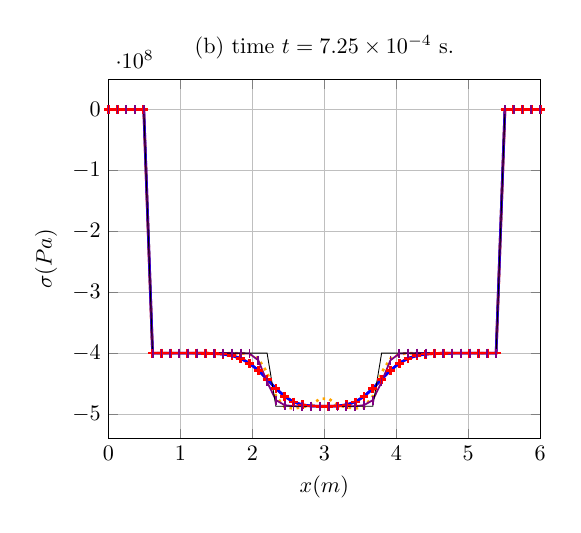
\begin{tikzpicture}[scale=0.8]
\begin{axis}[xlabel=$x (m)$,ylabel=$\sigma (Pa)$,ymajorgrids=true,xmajorgrids=true,legend pos=outer north east,title={(b) time $t = 7.25\times 10^{-4} $ s.},xmin=0.,xmax=6.]
\addplot[Red,very thick,mark=+,solid] coordinates {(0.0,-0.016398596440346053) (0.12244897959183673,-0.06425322857955201) (0.24489795918367346,-0.7380674881804443) (0.36734693877551017,-2.12047390173559) (0.4897959183673469,-28.76271861558054) (0.6122448979591837,-400000015.4159754) (0.7346938775510203,-400000102.7573024) (0.8571428571428571,-400000598.1932516) (0.9795918367346939,-400003055.79803795) (1.1020408163265305,-400013747.0436081) (1.2244897959183674,-400054602.7199052) (1.346938775510204,-400191823.2382515) (1.4693877551020407,-400596672.6802674) (1.5918367346938775,-401644186.51493835) (1.7142857142857142,-404014374.4754996) (1.836734693877551,-408684632.25449073) (1.9591836734693877,-416652037.9726774) (2.0816326530612246,-428329061.0045163) (2.204081632653061,-442879954.5361007) (2.326530612244898,-458084443.80872595) (2.4489795918367347,-471157539.9020842) (2.571428571428571,-480164339.19475454) (2.693877551020408,-484944715.5259052) (2.816326530612245,-486779650.5319825) (2.9387755102040813,-487233015.60471344) (3.061224489795918,-487233015.60471344) (3.183673469387755,-486779650.5319825) (3.306122448979592,-484944715.5259052) (3.4285714285714284,-480164339.19475454) (3.5510204081632653,-471157539.9020842) (3.673469387755102,-458084443.80872613) (3.7959183673469385,-442879954.5361007) (3.9183673469387754,-428329061.0045163) (4.040816326530612,-416652037.9726776) (4.163265306122449,-408684632.2544908) (4.285714285714286,-404014374.4754996) (4.408163265306122,-401644186.5149382) (4.530612244897959,-400596672.68026733) (4.653061224489796,-400191823.2382513) (4.775510204081632,-400054602.7199051) (4.8979591836734695,-400013747.04360807) (5.020408163265306,-400003055.79803795) (5.142857142857142,-400000598.19325155) (5.26530612244898,-400000102.75730234) (5.387755102040816,-400000015.4159754) (5.5102040816326525,-28.762718512303003) (5.63265306122449,-2.1204742438100417) (5.755102040816326,-0.7380675867576459) (5.877551020408163,-0.06425320166977637) (6.0,-0.01639854380134023) };
\addplot[Orange,very thick,mark=none,dotted] coordinates {(0.0011999999999999927,0.0) (0.12359999999999997,2.8345154836222343e-06) (0.24599999999999994,0.0) (0.36839999999999995,-5.6690309672444694e-06) (0.4907999999999999,5.563100179036459e-06) (0.6131999999999999,-400000000.00000036) (0.7355999999999999,-400000000.00000095) (0.858,-400000000.0000158) (0.9803999999999998,-400000000.000588) (1.1027999999999998,-400000000.0183558) (1.2251999999999996,-400000000.47669524) (1.3475999999999997,-400000010.242256) (1.4699999999999998,-400000180.58382314) (1.5923999999999996,-400002583.79875094) (1.7147999999999997,-400029558.11391515) (1.8371999999999995,-400265019.7421873) (1.9595999999999996,-401812442.4208182) (2.0819999999999994,-409100274.22059995) (2.2043999999999997,-431724216.84982246) (2.3267999999999995,-470516941.3021229) (2.4491999999999994,-488918339.55243546) (2.5715999999999997,-490903509.0666595) (2.6939999999999995,-488910392.160918) (2.8163999999999993,-485129466.2005724) (2.9387999999999996,-474875832.26573056) (3.0611999999999995,-474875832.26572955) (3.1835999999999993,-485129466.20057756) (3.305999999999999,-488910392.1609156) (3.4283999999999994,-490903509.0666595) (3.5507999999999993,-488918339.5524351) (3.673199999999999,-470516941.30212307) (3.7955999999999994,-431724216.8498228) (3.9179999999999993,-409100274.22060007) (4.040399999999999,-401812442.42081815) (4.1628,-400265019.742187) (4.2852,-400029558.11391526) (4.4076,-400002583.79875064) (4.53,-400000180.5838233) (4.6524,-400000010.242256) (4.7748,-400000000.47669554) (4.8972,-400000000.01835567) (5.0196,-400000000.00058854) (5.142,-400000000.00001574) (5.2644,-400000000.0000007) (5.3868,-400000000.0) (5.5092,-2.660415564296186e-06) (5.6316,-2.493917513477148e-06) (5.754,-2.7171818926536604e-06) (5.8764,3.405979701450893e-07) (5.9988,-2.8345154836222373e-06) };
\addplot[Blue,very thick,mark=none,solid] coordinates {(0.0011999999999999927,-0.00357849008468239) (0.12359999999999997,-0.06440079814818947) (0.24599999999999994,-0.21143910174666652) (0.36839999999999995,-2.1204748738318564) (0.4907999999999999,-3.2714037895202637) (0.6131999999999999,-400000015.4159753) (0.7355999999999999,-400000102.75730234) (0.858,-400000598.1932516) (0.9803999999999998,-400003055.79803795) (1.1027999999999998,-400013747.04360807) (1.2251999999999996,-400054602.7199051) (1.3475999999999997,-400191823.2382513) (1.4699999999999998,-400596672.68026733) (1.5923999999999996,-401644186.5149383) (1.7147999999999997,-404014374.47549963) (1.8371999999999995,-408684632.25449085) (1.9595999999999996,-416652037.9726776) (2.0819999999999994,-428329061.00451636) (2.2043999999999997,-442879954.5361008) (2.3267999999999995,-458084443.80872625) (2.4491999999999994,-471157539.9020842) (2.5715999999999997,-480164339.1947546) (2.6939999999999995,-484944715.52590525) (2.8163999999999993,-486779650.5319826) (2.9387999999999996,-487233015.60471344) (3.0611999999999995,-487233015.60471344) (3.1835999999999993,-486779650.5319826) (3.305999999999999,-484944715.52590525) (3.4283999999999994,-480164339.1947546) (3.5507999999999993,-471157539.9020842) (3.673199999999999,-458084443.80872625) (3.7955999999999994,-442879954.5361008) (3.9179999999999993,-428329061.00451636) (4.040399999999999,-416652037.9726776) (4.1628,-408684632.25449085) (4.2852,-404014374.47549963) (4.4076,-401644186.5149383) (4.53,-400596672.68026733) (4.6524,-400191823.2382513) (4.7748,-400054602.7199051) (4.8972,-400013747.04360807) (5.0196,-400003055.79803795) (5.142,-400000598.1932516) (5.2644,-400000102.75730234) (5.3868,-400000015.4159753) (5.5092,-3.2714037895202637) (5.6316,-2.1204748738318564) (5.754,-0.21143910174666652) (5.8764,-0.06440079814818947) (5.9988,-0.00357849008468239) };
\addplot[Purple,thick,mark=|,solid] coordinates {(0.0011999999999999927,1.6543612251060583e-24) (0.12359999999999997,1.6543612251060553e-23) (0.24599999999999994,2.452440800103604e-08) (0.36839999999999995,-3.508023677435457e-08) (0.4907999999999999,-5.960464477539063e-08) (0.6131999999999999,-400000000.0) (0.7355999999999999,-400000000.0) (0.858,-400000000.0000003) (0.9803999999999998,-400000000.0000133) (1.1027999999999998,-400000000.0004144) (1.2251999999999996,-400000000.0115142) (1.3475999999999997,-400000000.2871339) (1.4699999999999998,-400000006.46675307) (1.5923999999999996,-400000132.73197645) (1.7147999999999997,-400002510.7191475) (1.8371999999999995,-400043970.06492174) (1.9595999999999996,-400741455.361692) (2.0819999999999994,-411776022.67189264) (2.2043999999999997,-447347518.96724993) (2.3267999999999995,-477210124.05958325) (2.4491999999999994,-485453941.80645174) (2.5715999999999997,-487021615.6680456) (2.6939999999999995,-487258956.9032909) (2.8163999999999993,-487285223.6098061) (2.9387999999999996,-487287092.0986835) (3.0611999999999995,-487287092.0986835) (3.1835999999999993,-487285223.6098061) (3.305999999999999,-487258956.9032909) (3.4283999999999994,-487021615.6680456) (3.5507999999999993,-485453941.80645174) (3.673199999999999,-477210124.05958325) (3.7955999999999994,-447347518.96724993) (3.9179999999999993,-411776022.67189264) (4.040399999999999,-400741455.361692) (4.1628,-400043970.06492174) (4.2852,-400002510.71914756) (4.4076,-400000132.73197645) (4.53,-400000006.466753) (4.6524,-400000000.287134) (4.7748,-400000000.01151425) (4.8972,-400000000.0004144) (5.0196,-400000000.0000133) (5.142,-400000000.0000003) (5.2644,-400000000.0) (5.3868,-400000000.0) (5.5092,-5.960464477539063e-08) (5.6316,-3.508023677435457e-08) (5.754,2.452440800103604e-08) (5.8764,1.6543612251060553e-23) (5.9988,1.6543612251060583e-24) };
\addplot[black,thin,mark=none,solid] coordinates {(0.0,-0.0) (0.12244897959183673,-0.0) (0.24489795918367346,-0.0) (0.36734693877551017,-0.0) (0.4897959183673469,-0.0) (0.6122448979591837,-400000000.0) (0.7346938775510203,-400000000.0) (0.8571428571428571,-400000000.0) (0.9795918367346939,-400000000.0) (1.1020408163265305,-400000000.0) (1.2244897959183674,-400000000.0) (1.346938775510204,-400000000.0) (1.4693877551020407,-400000000.0) (1.5918367346938775,-400000000.0) (1.7142857142857142,-400000000.0) (1.836734693877551,-400000000.0) (1.9591836734693877,-400000000.0) (2.0816326530612246,-400000000.0) (2.204081632653061,-400000000.0) (2.326530612244898,-487287156.09439695) (2.4489795918367347,-487287156.09439695) (2.571428571428571,-487287156.09439695) (2.693877551020408,-487287156.09439695) (2.816326530612245,-487287156.09439695) (2.9387755102040813,-487287156.09439695) (3.061224489795918,-487287156.09439695) (3.183673469387755,-487287156.09439695) (3.306122448979592,-487287156.09439695) (3.4285714285714284,-487287156.09439695) (3.5510204081632653,-487287156.09439695) (3.673469387755102,-487287156.09439695) (3.7959183673469385,-400000000.0) (3.9183673469387754,-400000000.0) (4.040816326530612,-400000000.0) (4.163265306122449,-400000000.0) (4.285714285714286,-400000000.0) (4.408163265306122,-400000000.0) (4.530612244897959,-400000000.0) (4.653061224489796,-400000000.0) (4.775510204081632,-400000000.0) (4.8979591836734695,-400000000.0) (5.020408163265306,-400000000.0) (5.142857142857142,-400000000.0) (5.26530612244898,-400000000.0) (5.387755102040816,-400000000.0) (5.5102040816326525,-0.0) (5.63265306122449,-0.0) (5.755102040816326,-0.0) (5.877551020408163,-0.0) (6.0,-0.0) };
%\legend{dgmpm,fem,fvm,fvm (SB),exact}
\end{axis}
\end{tikzpicture}
%%% Local Variables:
%%% mode: latex
%%% TeX-master: "../../mainManuscript"
%%% End:
}
  {\begin{tikzpicture}[scale=.9]
\begin{groupplot}[group style={group size=3 by 2,
ylabels at=edge left, yticklabels at=edge left,horizontal sep=2.ex,
vertical sep=4ex,xticklabels at=edge bottom,xlabels at=edge bottom},
ymajorgrids=true,xmajorgrids=true,enlargelimits=0,xmin=0.,xmax=6.,xlabel=$x (m)$,
axis on top,scale only axis,width=0.32\linewidth
]
\nextgroupplot[title={(a) $t = 4.17\times 10^{-4} $ s.},ymin=-1490030330.3270838,ymax=192511976.64755264,]
\addplot[Red,solid,mark=+,very thick,mark size=3pt,mark repeat=2] coordinates{(0.0,-3.2561158711216654e-07) (0.12244897959183673,-6.54162606232603e-22) (0.24489795918367346,0.0) (0.36734693877551017,3.2561158711216643e-07) (0.4897959183673469,-4.884173806682499e-07) (0.6122448979591837,-706703995.0062007) (0.7346938775510203,-739923853.3127105) (0.8571428571428571,-818114621.3278772) (0.9795918367346939,-934350667.0858994) (1.1020408163265305,-1056745717.4113452) (1.2244897959183674,-1153785079.176232) (1.346938775510204,-1213891661.9862223) (1.4693877551020407,-1243675875.166416) (1.5918367346938775,-1255667377.4619899) (1.7142857142857142,-1259628756.7765899) (1.836734693877551,-1260708382.472525) (1.9591836734693877,-1260951555.06527) (2.0816326530612246,-1260996741.6987677) (2.204081632653061,-1261003631.246593) (2.326530612244898,-1261004484.7294881) (2.4489795918367347,-1261004569.3136225) (2.571428571428571,-1261004575.8625927) (2.693877551020408,-1261004576.2443771) (2.816326530612245,-1261004576.2601426) (2.9387755102040813,-1261004576.2605536) (3.061224489795918,-1261004576.2605536) (3.183673469387755,-1261004576.2601426) (3.306122448979592,-1261004576.2443776) (3.4285714285714284,-1261004575.862593) (3.5510204081632653,-1261004569.3136227) (3.673469387755102,-1261004484.7294881) (3.7959183673469385,-1261003631.2465928) (3.9183673469387754,-1260996741.6987677) (4.040816326530612,-1260951555.0652697) (4.163265306122449,-1260708382.4725246) (4.285714285714286,-1259628756.7765894) (4.408163265306122,-1255667377.4619899) (4.530612244897959,-1243675875.1664157) (4.653061224489796,-1213891661.9862223) (4.775510204081632,-1153785079.176232) (4.8979591836734695,-1056745717.4113454) (5.020408163265306,-934350667.0858992) (5.142857142857142,-818114621.327877) (5.26530612244898,-739923853.3127109) (5.387755102040816,-706703995.0062011) (5.5102040816326525,-4.884173806682498e-07) (5.63265306122449,0.0) (5.755102040816326,-4.884173806682498e-07) (5.877551020408163,0.0) (6.0,-4.884173806682498e-07) };
\addplot[Orange,dotted,mark=none,very thick,mark size=3pt,mark repeat=2] coordinates{(0.0,0.0) (0.12244897959183673,0.0) (0.24489795918367346,0.0) (0.36734693877551017,0.0) (0.4897959183673469,0.0) (0.6122448979591837,-700099961.461325) (0.7346938775510203,-702215400.6707044) (0.8571428571428571,-720845446.6905135) (0.9795918367346939,-807249777.2239016) (1.1020408163265305,-1021817726.088786) (1.2244897959183674,-1257135415.8766613) (1.346938775510204,-1201909815.2742617) (1.4693877551020407,-1284541316.0967622) (1.5918367346938775,-1197762497.5853782) (1.7142857142857142,-1280230396.1356874) (1.836734693877551,-1230639248.475009) (1.9591836734693877,-1232614670.2907715) (2.0816326530612246,-1296340561.1434355) (2.204081632653061,-1163180742.3691304) (2.326530612244898,-1344085453.2920678) (2.4489795918367347,-1125286993.986051) (2.571428571428571,-1354573027.5700727) (2.693877551020408,-1144440690.6862848) (2.816326530612245,-1331966839.3238678) (2.9387755102040813,-1234245710.8866477) (3.061224489795918,-1234245710.8866642) (3.183673469387755,-1331966839.3238637) (3.306122448979592,-1144440690.6862931) (3.4285714285714284,-1354573027.570076) (3.5510204081632653,-1125286993.9860492) (3.673469387755102,-1344085453.2920709) (3.7959183673469385,-1163180742.369132) (3.9183673469387754,-1296340561.143439) (4.040816326530612,-1232614670.2907667) (4.163265306122449,-1230639248.4750104) (4.285714285714286,-1280230396.1356888) (4.408163265306122,-1197762497.5853772) (4.530612244897959,-1284541316.0967634) (4.653061224489796,-1201909815.2742698) (4.775510204081632,-1257135415.8766532) (4.8979591836734695,-1021817726.0887933) (5.020408163265306,-807249777.2238963) (5.142857142857142,-720845446.6905184) (5.26530612244898,-702215400.6706979) (5.387755102040816,-700099961.4613259) (5.5102040816326525,0.0) (5.63265306122449,0.0) (5.755102040816326,0.0) (5.877551020408163,0.0) (6.0,0.0) };
\addplot[Blue,solid,mark=none,very thick,mark size=3pt,mark repeat=2] coordinates{(0.0,0.0) (0.12244897959183673,0.0) (0.24489795918367346,0.0) (0.36734693877551017,0.0) (0.4897959183673469,0.0) (0.6122448979591837,-706703995.0062009) (0.7346938775510203,-739923853.3127103) (0.8571428571428571,-818114621.3278768) (0.9795918367346939,-934350667.085899) (1.1020408163265305,-1056745717.4113449) (1.2244897959183674,-1153785079.176232) (1.346938775510204,-1213891661.9862218) (1.4693877551020407,-1243675875.1664155) (1.5918367346938775,-1255667377.4619896) (1.7142857142857142,-1259628756.7765894) (1.836734693877551,-1260708382.4725244) (1.9591836734693877,-1260951555.06527) (2.0816326530612246,-1260996741.6987672) (2.204081632653061,-1261003631.246593) (2.326530612244898,-1261004484.7294877) (2.4489795918367347,-1261004569.3136225) (2.571428571428571,-1261004575.862593) (2.693877551020408,-1261004576.2443774) (2.816326530612245,-1261004576.2601426) (2.9387755102040813,-1261004576.2605534) (3.061224489795918,-1261004576.2605536) (3.183673469387755,-1261004576.2601426) (3.306122448979592,-1261004576.2443774) (3.4285714285714284,-1261004575.862593) (3.5510204081632653,-1261004569.3136225) (3.673469387755102,-1261004484.729488) (3.7959183673469385,-1261003631.246593) (3.9183673469387754,-1260996741.6987672) (4.040816326530612,-1260951555.06527) (4.163265306122449,-1260708382.4725244) (4.285714285714286,-1259628756.7765892) (4.408163265306122,-1255667377.4619894) (4.530612244897959,-1243675875.1664155) (4.653061224489796,-1213891661.9862218) (4.775510204081632,-1153785079.1762319) (4.8979591836734695,-1056745717.4113448) (5.020408163265306,-934350667.0858989) (5.142857142857142,-818114621.3278767) (5.26530612244898,-739923853.3127103) (5.387755102040816,-706703995.0062009) (5.5102040816326525,0.0) (5.63265306122449,0.0) (5.755102040816326,0.0) (5.877551020408163,0.0) (6.0,0.0) };
\addplot[Purple,solid,mark=x,thick,mark size=3pt,mark repeat=2] coordinates{(0.0,0.0) (0.12244897959183673,0.0) (0.24489795918367346,0.0) (0.36734693877551017,0.0) (0.4897959183673469,0.0) (0.6122448979591837,-700149009.8511133) (0.7346938775510203,-702792255.866507) (0.8571428571428571,-725326867.326901) (0.9795918367346939,-850156660.8530495) (1.1020408163265305,-1109984935.9712873) (1.2244897959183674,-1250258832.4370122) (1.346938775510204,-1260471082.9558206) (1.4693877551020407,-1260981625.9873586) (1.5918367346938775,-1261003693.8957453) (1.7142857142857142,-1261004546.9659622) (1.836734693877551,-1261004575.4299965) (1.9591836734693877,-1261004576.2405941) (2.0816326530612246,-1261004576.260158) (2.204081632653061,-1261004576.2605524) (2.326530612244898,-1261004576.260559) (2.4489795918367347,-1261004576.260559) (2.571428571428571,-1261004576.260559) (2.693877551020408,-1261004576.260559) (2.816326530612245,-1261004576.2605588) (2.9387755102040813,-1261004576.2605588) (3.061224489795918,-1261004576.260559) (3.183673469387755,-1261004576.2605588) (3.306122448979592,-1261004576.2605588) (3.4285714285714284,-1261004576.2605588) (3.5510204081632653,-1261004576.2605588) (3.673469387755102,-1261004576.2605588) (3.7959183673469385,-1261004576.260553) (3.9183673469387754,-1261004576.2601585) (4.040816326530612,-1261004576.2405944) (4.163265306122449,-1261004575.4299967) (4.285714285714286,-1261004546.9659626) (4.408163265306122,-1261003693.895745) (4.530612244897959,-1260981625.987358) (4.653061224489796,-1260471082.955823) (4.775510204081632,-1250258832.4370096) (4.8979591836734695,-1109984935.971287) (5.020408163265306,-850156660.8530501) (5.142857142857142,-725326867.326901) (5.26530612244898,-702792255.866507) (5.387755102040816,-700149009.8511133) (5.5102040816326525,0.0) (5.63265306122449,0.0) (5.755102040816326,0.0) (5.877551020408163,0.0) (6.0,0.0) };
\addplot[black,solid,mark=none,thin,mark size=3pt,mark repeat=2] coordinates{(0.0,-0.0) (0.12244897959183673,-0.0) (0.24489795918367346,-0.0) (0.36734693877551017,-0.0) (0.4897959183673469,-0.0) (0.6122448979591837,-700000000.0) (0.7346938775510203,-700000000.0) (0.8571428571428571,-700000000.0) (0.9795918367346939,-700000000.0) (1.1020408163265305,-1261004576.260559) (1.2244897959183674,-1261004576.260559) (1.346938775510204,-1261004576.260559) (1.4693877551020407,-1261004576.260559) (1.5918367346938775,-1261004576.260559) (1.7142857142857142,-1261004576.260559) (1.836734693877551,-1261004576.260559) (1.9591836734693877,-1261004576.260559) (2.0816326530612246,-1261004576.260559) (2.204081632653061,-1261004576.260559) (2.326530612244898,-1261004576.260559) (2.4489795918367347,-1261004576.260559) (2.571428571428571,-1261004576.260559) (2.693877551020408,-1261004576.260559) (2.816326530612245,-1261004576.260559) (2.9387755102040813,-1261004576.260559) (3.061224489795918,-1261004576.260559) (3.183673469387755,-1261004576.260559) (3.306122448979592,-1261004576.260559) (3.4285714285714284,-1261004576.260559) (3.5510204081632653,-1261004576.260559) (3.673469387755102,-1261004576.260559) (3.7959183673469385,-1261004576.260559) (3.9183673469387754,-1261004576.260559) (4.040816326530612,-1261004576.260559) (4.163265306122449,-1261004576.260559) (4.285714285714286,-1261004576.260559) (4.408163265306122,-1261004576.260559) (4.530612244897959,-1261004576.260559) (4.653061224489796,-1261004576.260559) (4.775510204081632,-1261004576.260559) (4.8979591836734695,-1261004576.260559) (5.020408163265306,-700000000.0) (5.142857142857142,-700000000.0) (5.26530612244898,-700000000.0) (5.387755102040816,-700000000.0) (5.5102040816326525,-0.0) (5.63265306122449,-0.0) (5.755102040816326,-0.0) (5.877551020408163,-0.0) (6.0,-0.0) };
\nextgroupplot[title={(b) $t = 6.25\times 10^{-4} $ s.},ymin=-1490030330.3270838,ymax=192511976.64755264,]
\addplot[Red,solid,mark=+,very thick,mark size=3pt,mark repeat=2] coordinates{(0.0,-120597397.19248778) (0.12244897959183673,-298539345.15508544) (0.24489795918367346,-464504460.170754) (0.36734693877551017,-546627376.3559334) (0.4897959183673469,-635546108.2543886) (0.6122448979591837,-1247334335.3333962) (0.7346938775510203,-1255980074.5990539) (0.8571428571428571,-1259371705.5275755) (0.9795918367346939,-1260535220.1287405) (1.1020408163265305,-1260885267.5005968) (1.2244897959183674,-1260977777.705495) (1.346938775510204,-1260999265.6570995) (1.4693877551020407,-1261003650.0375175) (1.5918367346938775,-1261004434.5740557) (1.7142857142857142,-1261004557.3391547) (1.836734693877551,-1261004574.0682204) (1.9591836734693877,-1261004576.0419452) (2.0816326530612246,-1261004576.241996) (2.204081632653061,-1261004576.2592359) (2.326530612244898,-1261004576.260481) (2.4489795918367347,-1261004576.260556) (2.571428571428571,-1261004576.2605588) (2.693877551020408,-1261004576.260559) (2.816326530612245,-1261004576.2605588) (2.9387755102040813,-1261004576.260559) (3.061224489795918,-1261004576.2605584) (3.183673469387755,-1261004576.2605586) (3.306122448979592,-1261004576.2605588) (3.4285714285714284,-1261004576.2605581) (3.5510204081632653,-1261004576.2605555) (3.673469387755102,-1261004576.260481) (3.7959183673469385,-1261004576.2592354) (3.9183673469387754,-1261004576.2419953) (4.040816326530612,-1261004576.0419443) (4.163265306122449,-1261004574.06822) (4.285714285714286,-1261004557.3391542) (4.408163265306122,-1261004434.5740552) (4.530612244897959,-1261003650.037517) (4.653061224489796,-1260999265.6570988) (4.775510204081632,-1260977777.7054946) (4.8979591836734695,-1260885267.500596) (5.020408163265306,-1260535220.1287398) (5.142857142857142,-1259371705.5275738) (5.26530612244898,-1255980074.5990536) (5.387755102040816,-1247334335.3333952) (5.5102040816326525,-635546108.2543867) (5.63265306122449,-546627376.3559326) (5.755102040816326,-464504460.1707534) (5.877551020408163,-298539345.15508515) (6.0,-120597397.19248791) };
\addplot[Orange,dotted,mark=none,very thick,mark size=3pt,mark repeat=2] coordinates{(0.0,-176853791.94554004) (0.12244897959183673,-378394340.717152) (0.24489795918367346,-693239198.8311979) (0.36734693877551017,-523439989.89111507) (0.4897959183673469,-693552985.1722431) (0.6122448979591837,-1243921088.325841) (0.7346938775510203,-1243896835.4237814) (0.8571428571428571,-1238512519.7129703) (0.9795918367346939,-1242876003.1599257) (1.1020408163265305,-1229134621.6433644) (1.2244897959183674,-1260098267.149167) (1.346938775510204,-1238022210.520185) (1.4693877551020407,-1269111852.1192086) (1.5918367346938775,-1241379610.2251832) (1.7142857142857142,-1289870286.8459477) (1.836734693877551,-1207539167.6018116) (1.9591836734693877,-1302352875.6492124) (2.0816326530612246,-1179646467.1836338) (2.204081632653061,-1302099080.7920847) (2.326530612244898,-1195754724.162506) (2.4489795918367347,-1294783662.9363751) (2.571428571428571,-1223699568.3092146) (2.693877551020408,-1275816869.6395779) (2.816326530612245,-1243094391.3994842) (2.9387755102040813,-1250401942.2614183) (3.061224489795918,-1250401942.2613835) (3.183673469387755,-1243094391.3995185) (3.306122448979592,-1275816869.6395504) (3.4285714285714284,-1223699568.3092418) (3.5510204081632653,-1294783662.9363482) (3.673469387755102,-1195754724.16253) (3.7959183673469385,-1302099080.7920847) (3.9183673469387754,-1179646467.1836205) (4.040816326530612,-1302352875.6492195) (4.163265306122449,-1207539167.601786) (4.285714285714286,-1289870286.8459682) (4.408163265306122,-1241379610.2251687) (4.530612244897959,-1269111852.1192243) (4.653061224489796,-1238022210.5201812) (4.775510204081632,-1260098267.1491652) (4.8979591836734695,-1229134621.643366) (5.020408163265306,-1242876003.159929) (5.142857142857142,-1238512519.712955) (5.26530612244898,-1243896835.4238017) (5.387755102040816,-1243921088.3258262) (5.5102040816326525,-693552985.1722746) (5.63265306122449,-523439989.8910899) (5.755102040816326,-693239198.8312114) (5.877551020408163,-378394340.71715474) (6.0,-176853791.9455247) };
\addplot[Blue,solid,mark=none,very thick,mark size=3pt,mark repeat=2] coordinates{(0.0,-96650988.15728289) (0.12244897959183673,-314215597.0101885) (0.24489795918367346,-447225867.04361707) (0.36734693877551017,-549691260.4581364) (0.4897959183673469,-561200942.1999743) (0.6122448979591837,-1247334335.3333952) (0.7346938775510203,-1255980074.5990531) (0.8571428571428571,-1259371705.5275743) (0.9795918367346939,-1260535220.1287396) (1.1020408163265305,-1260885267.5005958) (1.2244897959183674,-1260977777.7054944) (1.346938775510204,-1260999265.6570985) (1.4693877551020407,-1261003650.037517) (1.5918367346938775,-1261004434.5740547) (1.7142857142857142,-1261004557.3391533) (1.836734693877551,-1261004574.0682194) (1.9591836734693877,-1261004576.041944) (2.0816326530612246,-1261004576.2419949) (2.204081632653061,-1261004576.259235) (2.326530612244898,-1261004576.260481) (2.4489795918367347,-1261004576.2605555) (2.571428571428571,-1261004576.2605588) (2.693877551020408,-1261004576.2605588) (2.816326530612245,-1261004576.2605588) (2.9387755102040813,-1261004576.260559) (3.061224489795918,-1261004576.2605588) (3.183673469387755,-1261004576.260559) (3.306122448979592,-1261004576.260559) (3.4285714285714284,-1261004576.260559) (3.5510204081632653,-1261004576.2605555) (3.673469387755102,-1261004576.2604809) (3.7959183673469385,-1261004576.2592351) (3.9183673469387754,-1261004576.241995) (4.040816326530612,-1261004576.041944) (4.163265306122449,-1261004574.0682197) (4.285714285714286,-1261004557.3391535) (4.408163265306122,-1261004434.5740547) (4.530612244897959,-1261003650.0375168) (4.653061224489796,-1260999265.6570985) (4.775510204081632,-1260977777.7054942) (4.8979591836734695,-1260885267.5005958) (5.020408163265306,-1260535220.1287396) (5.142857142857142,-1259371705.5275743) (5.26530612244898,-1255980074.5990531) (5.387755102040816,-1247334335.333395) (5.5102040816326525,-561200942.1999743) (5.63265306122449,-549691260.4581364) (5.755102040816326,-447225867.0436171) (5.877551020408163,-314215597.0101884) (6.0,-96650988.15728283) };
\addplot[Purple,solid,mark=x,thick,mark size=3pt,mark repeat=2] coordinates{(0.0,-178085389.46677893) (0.12244897959183673,-530375739.95348394) (0.24489795918367346,-606212710.479109) (0.36734693877551017,-629775762.9786947) (0.4897959183673469,-602317892.3964041) (0.6122448979591837,-1261002720.0436904) (0.7346938775510203,-1261004493.0577958) (0.8571428571428571,-1261004572.8496082) (0.9795918367346939,-1261004576.1336117) (1.1020408163265305,-1261004576.256299) (1.2244897959183674,-1261004576.2604308) (1.346938775510204,-1261004576.2605557) (1.4693877551020407,-1261004576.260559) (1.5918367346938775,-1261004576.2605586) (1.7142857142857142,-1261004576.2605586) (1.836734693877551,-1261004576.260559) (1.9591836734693877,-1261004576.260559) (2.0816326530612246,-1261004576.2605586) (2.204081632653061,-1261004576.2605588) (2.326530612244898,-1261004576.2605588) (2.4489795918367347,-1261004576.2605588) (2.571428571428571,-1261004576.2605586) (2.693877551020408,-1261004576.2605588) (2.816326530612245,-1261004576.2605586) (2.9387755102040813,-1261004576.2605588) (3.061224489795918,-1261004576.2605588) (3.183673469387755,-1261004576.260559) (3.306122448979592,-1261004576.2605584) (3.4285714285714284,-1261004576.2605584) (3.5510204081632653,-1261004576.2605586) (3.673469387755102,-1261004576.2605588) (3.7959183673469385,-1261004576.2605588) (3.9183673469387754,-1261004576.260559) (4.040816326530612,-1261004576.2605586) (4.163265306122449,-1261004576.2605588) (4.285714285714286,-1261004576.2605586) (4.408163265306122,-1261004576.2605586) (4.530612244897959,-1261004576.2605586) (4.653061224489796,-1261004576.2605553) (4.775510204081632,-1261004576.2604303) (4.8979591836734695,-1261004576.2562997) (5.020408163265306,-1261004576.133612) (5.142857142857142,-1261004572.8496091) (5.26530612244898,-1261004493.0577967) (5.387755102040816,-1261002720.0436902) (5.5102040816326525,-602317892.3964037) (5.63265306122449,-629775762.9786928) (5.755102040816326,-606212710.4791106) (5.877551020408163,-530375739.9534838) (6.0,-178085389.4667765) };
\addplot[black,solid,mark=none,thin,mark size=3pt,mark repeat=2] coordinates{(0.0,-0.0) (0.12244897959183673,-630502288.1302795) (0.24489795918367346,-630502288.1302795) (0.36734693877551017,-630502288.1302795) (0.4897959183673469,-630502288.1302795) (0.6122448979591837,-1261004576.260559) (0.7346938775510203,-1261004576.260559) (0.8571428571428571,-1261004576.260559) (0.9795918367346939,-1261004576.260559) (1.1020408163265305,-1261004576.260559) (1.2244897959183674,-1261004576.260559) (1.346938775510204,-1261004576.260559) (1.4693877551020407,-1261004576.260559) (1.5918367346938775,-1261004576.260559) (1.7142857142857142,-1261004576.260559) (1.836734693877551,-1261004576.260559) (1.9591836734693877,-1261004576.260559) (2.0816326530612246,-1261004576.260559) (2.204081632653061,-1261004576.260559) (2.326530612244898,-1261004576.260559) (2.4489795918367347,-1261004576.260559) (2.571428571428571,-1261004576.260559) (2.693877551020408,-1261004576.260559) (2.816326530612245,-1261004576.260559) (2.9387755102040813,-1261004576.260559) (3.061224489795918,-1261004576.260559) (3.183673469387755,-1261004576.260559) (3.306122448979592,-1261004576.260559) (3.4285714285714284,-1261004576.260559) (3.5510204081632653,-1261004576.260559) (3.673469387755102,-1261004576.260559) (3.7959183673469385,-1261004576.260559) (3.9183673469387754,-1261004576.260559) (4.040816326530612,-1261004576.260559) (4.163265306122449,-1261004576.260559) (4.285714285714286,-1261004576.260559) (4.408163265306122,-1261004576.260559) (4.530612244897959,-1261004576.260559) (4.653061224489796,-1261004576.260559) (4.775510204081632,-1261004576.260559) (4.8979591836734695,-1261004576.260559) (5.020408163265306,-1261004576.260559) (5.142857142857142,-1261004576.260559) (5.26530612244898,-1261004576.260559) (5.387755102040816,-1261004576.260559) (5.5102040816326525,-630502288.1302795) (5.63265306122449,-630502288.1302795) (5.755102040816326,-630502288.1302795) (5.877551020408163,-630502288.1302795) (6.0,-0.0) };
\nextgroupplot[title={(c) $t = 9.38\times 10^{-4} $ s.},ymin=-1490030330.3270838,ymax=192511976.64755264,]
\addplot[Red,solid,mark=+,very thick,mark size=3pt,mark repeat=2] coordinates{(0.0,-288.000337932026) (0.12244897959183673,-2340.8049612902105) (0.24489795918367346,-6717.6736351549625) (0.36734693877551017,-31436.18543893099) (0.4897959183673469,-82819.9714218378) (0.6122448979591837,-326370.9123286009) (0.7346938775510203,-787154.078435719) (0.8571428571428571,-2592039.5752673745) (0.9795918367346939,-5646941.091449976) (1.1020408163265305,-15363721.703147352) (1.2244897959183674,-29743749.637923777) (1.346938775510204,-65953645.19968498) (1.4693877551020407,-111309952.15841854) (1.5918367346938775,-198327314.7707913) (1.7142857142857142,-286130814.5665431) (1.836734693877551,-406728211.7590317) (1.9591836734693877,-496866659.92587715) (2.0816326530612246,-575814412.3291717) (2.204081632653061,-612581021.5556204) (2.326530612244898,-666589640.9783571) (2.4489795918367347,-1261004576.260559) (2.571428571428571,-1261004576.2605588) (2.693877551020408,-1261004576.2605588) (2.816326530612245,-1261004576.260559) (2.9387755102040813,-1261004576.260559) (3.061224489795918,-1261004576.2605588) (3.183673469387755,-1261004576.2605588) (3.306122448979592,-1261004576.2605586) (3.4285714285714284,-1261004576.260559) (3.5510204081632653,-1261004576.2605588) (3.673469387755102,-666589640.9783564) (3.7959183673469385,-612581021.5556185) (3.9183673469387754,-575814412.3291717) (4.040816326530612,-496866659.92587644) (4.163265306122449,-406728211.7590302) (4.285714285714286,-286130814.5665426) (4.408163265306122,-198327314.77079123) (4.530612244897959,-111309952.15841806) (4.653061224489796,-65953645.19968575) (4.775510204081632,-29743749.637924016) (4.8979591836734695,-15363721.703146577) (5.020408163265306,-5646941.091449976) (5.142857142857142,-2592039.5752685666) (5.26530612244898,-787154.0784354806) (5.387755102040816,-326370.91232824326) (5.5102040816326525,-82819.97142159939) (5.63265306122449,-31436.185439646244) (5.755102040816326,-6717.673635229468) (5.877551020408163,-2340.804961979389) (6.0,-288.00033782143146) };
\addplot[Orange,dotted,mark=none,very thick,mark size=3pt,mark repeat=2] coordinates{(0.0,175010887.86141148) (0.12244897959183673,-157010320.72319484) (0.24489795918367346,157731015.99830914) (0.36734693877551017,-141347084.0250168) (0.4897959183673469,117914146.10742596) (0.6122448979591837,-112262666.61428112) (0.7346938775510203,51745557.76652613) (0.8571428571428571,-67268258.78012908) (0.9795918367346939,25135893.71762538) (1.1020408163265305,-51161038.25586742) (1.2244897959183674,38244096.87732005) (1.346938775510204,-71286114.06399637) (1.4693877551020407,42529781.300441384) (1.5918367346938775,-256057713.884533) (1.7142857142857142,-344993293.7306862) (1.836734693877551,-602082756.2554108) (1.9591836734693877,-551416188.3408538) (2.0816326530612246,-667542863.5679615) (2.204081632653061,-569236978.9147782) (2.326530612244898,-673381420.6974866) (2.4489795918367347,-1276652083.3178082) (2.571428571428571,-1242412632.5978575) (2.693877551020408,-1262303877.9393654) (2.816326530612245,-1245296647.9512377) (2.9387755102040813,-1251720925.4068818) (3.061224489795918,-1251720925.406923) (3.183673469387755,-1245296647.951198) (3.306122448979592,-1262303877.9393706) (3.4285714285714284,-1242412632.5978665) (3.5510204081632653,-1276652083.3177838) (3.673469387755102,-673381420.6975331) (3.7959183673469385,-569236978.9147345) (3.9183673469387754,-667542863.5679996) (4.040816326530612,-551416188.3408496) (4.163265306122449,-602082756.2553713) (4.285714285714286,-344993293.7307386) (4.408163265306122,-256057713.88448328) (4.530612244897959,42529781.300438166) (4.653061224489796,-71286114.06398582) (4.775510204081632,38244096.877307296) (4.8979591836734695,-51161038.2558347) (5.020408163265306,25135893.71758467) (5.142857142857142,-67268258.78007948) (5.26530612244898,51745557.766474634) (5.387755102040816,-112262666.6142239) (5.5102040816326525,117914146.10736191) (5.63265306122449,-141347084.02495122) (5.755102040816326,157731015.9982485) (5.877551020408163,-157010320.7231324) (6.0,175010887.86135092) };
\addplot[Blue,solid,mark=none,very thick,mark size=3pt,mark repeat=2] coordinates{(0.0,-672.000788774134) (0.12244897959183673,-2317.190485430212) (0.24489795918367346,-11624.7450740413) (0.36734693877551017,-31435.028274873635) (0.4897959183673469,-131180.5918317446) (0.6122448979591837,-326370.86669091054) (0.7346938775510203,-1145540.9690250745) (0.8571428571428571,-2592039.5738099255) (0.9795918367346939,-7576352.574992208) (1.1020408163265305,-15363721.703109615) (1.2244897959183674,-36933763.60530679) (1.346938775510204,-65953645.19968625) (1.4693877551020407,-128588545.2855558) (1.5918367346938775,-198327314.77079248) (1.7142857142857142,-310077223.60174906) (1.836734693877551,-406728211.759032) (1.9591836734693877,-512542911.78098124) (2.0816326530612246,-575814412.329173) (2.204081632653061,-615644905.6578237) (2.326530612244898,-597093014.0061195) (2.4489795918367347,-1261004576.2605588) (2.571428571428571,-1261004576.2605586) (2.693877551020408,-1261004576.2605588) (2.816326530612245,-1261004576.2605584) (2.9387755102040813,-1261004576.2605588) (3.061224489795918,-1261004576.2605586) (3.183673469387755,-1261004576.2605586) (3.306122448979592,-1261004576.2605586) (3.4285714285714284,-1261004576.2605588) (3.5510204081632653,-1261004576.2605584) (3.673469387755102,-597093014.0061196) (3.7959183673469385,-615644905.6578233) (3.9183673469387754,-575814412.329173) (4.040816326530612,-512542911.78098106) (4.163265306122449,-406728211.759032) (4.285714285714286,-310077223.601749) (4.408163265306122,-198327314.77079242) (4.530612244897959,-128588545.28555562) (4.653061224489796,-65953645.199686386) (4.775510204081632,-36933763.60530707) (4.8979591836734695,-15363721.703109678) (5.020408163265306,-7576352.5749919815) (5.142857142857142,-2592039.5738102393) (5.26530612244898,-1145540.9690254903) (5.387755102040816,-326370.8666910869) (5.5102040816326525,-131180.5918318261) (5.63265306122449,-31435.028275203294) (5.755102040816326,-11624.74507411075) (5.877551020408163,-2317.1904855701214) (6.0,-672.0007888251785) };
\addplot[Purple,solid,mark=x,thick,mark size=3pt,mark repeat=2] coordinates{(0.0,-2.2554342869669835e-07) (0.12244897959183673,-4.253451172600671e-07) (0.24489795918367346,-1.2920591556701192e-05) (0.36734693877551017,-5.986342632906781e-05) (0.4897959183673469,-0.0056401329400634255) (0.6122448979591837,-0.02444787812144389) (0.7346938775510203,-1.8760696294301331) (0.8571428571428571,-7.9566149629172855) (0.9795918367346939,-503.4524595203254) (1.1020408163265305,-2086.1665527314763) (1.2244897959183674,-111480.01946610014) (1.346938775510204,-452326.4024975486) (1.4693877551020407,-21130457.36149759) (1.5918367346938775,-83990511.6868726) (1.7142857142857142,-358373061.4587475) (1.836734693877551,-536458450.92552686) (1.9591836734693877,-614366251.640357) (2.0816326530612246,-627343167.840607) (2.204081632653061,-630228089.3811917) (2.326530612244898,-602429197.2873981) (2.4489795918367347,-1261004576.2605584) (2.571428571428571,-1261004576.2605586) (2.693877551020408,-1261004576.2605581) (2.816326530612245,-1261004576.2605586) (2.9387755102040813,-1261004576.2605584) (3.061224489795918,-1261004576.2605586) (3.183673469387755,-1261004576.2605584) (3.306122448979592,-1261004576.2605588) (3.4285714285714284,-1261004576.2605584) (3.5510204081632653,-1261004576.2605586) (3.673469387755102,-602429197.287398) (3.7959183673469385,-630228089.3811923) (3.9183673469387754,-627343167.8406069) (4.040816326530612,-614366251.6403568) (4.163265306122449,-536458450.9255258) (4.285714285714286,-358373061.45874953) (4.408163265306122,-83990511.68687272) (4.530612244897959,-21130457.361496225) (4.653061224489796,-452326.4024989642) (4.775510204081632,-111480.01946637034) (4.8979591836734695,-2086.166552579263) (5.020408163265306,-503.4524587330095) (5.142857142857142,-7.956613651988789) (5.26530612244898,-1.8760695971344141) (5.387755102040816,-0.024446596221118888) (5.5102040816326525,-0.005640085558921308) (5.63265306122449,-6.008348006163438e-05) (5.755102040816326,-1.352714115819129e-05) (5.877551020408163,-1.6124271861316672e-09) (6.0,-1.7267558828412451e-07) };
\addplot[black,solid,mark=none,thin,mark size=3pt,mark repeat=2] coordinates{(0.0,-0.0) (0.12244897959183673,-0.0) (0.24489795918367346,-0.0) (0.36734693877551017,-0.0) (0.4897959183673469,-0.0) (0.6122448979591837,-0.0) (0.7346938775510203,-0.0) (0.8571428571428571,-0.0) (0.9795918367346939,-0.0) (1.1020408163265305,-0.0) (1.2244897959183674,-0.0) (1.346938775510204,-0.0) (1.4693877551020407,-0.0) (1.5918367346938775,-0.0) (1.7142857142857142,-0.0) (1.836734693877551,-630502288.1302795) (1.9591836734693877,-630502288.1302795) (2.0816326530612246,-630502288.1302795) (2.204081632653061,-630502288.1302795) (2.326530612244898,-630502288.1302795) (2.4489795918367347,-1261004576.260559) (2.571428571428571,-1261004576.260559) (2.693877551020408,-1261004576.260559) (2.816326530612245,-1261004576.260559) (2.9387755102040813,-1261004576.260559) (3.061224489795918,-1261004576.260559) (3.183673469387755,-1261004576.260559) (3.306122448979592,-1261004576.260559) (3.4285714285714284,-1261004576.260559) (3.5510204081632653,-1261004576.260559) (3.673469387755102,-630502288.1302795) (3.7959183673469385,-630502288.1302795) (3.9183673469387754,-630502288.1302795) (4.040816326530612,-630502288.1302795) (4.163265306122449,-630502288.1302795) (4.285714285714286,-0.0) (4.408163265306122,-0.0) (4.530612244897959,-0.0) (4.653061224489796,-0.0) (4.775510204081632,-0.0) (4.8979591836734695,-0.0) (5.020408163265306,-0.0) (5.142857142857142,-0.0) (5.26530612244898,-0.0) (5.387755102040816,-0.0) (5.5102040816326525,-0.0) (5.63265306122449,-0.0) (5.755102040816326,-0.0) (5.877551020408163,-0.0) (6.0,-0.0) };
\nextgroupplot[ylabel=$\eps^p $,ymin=-0.002673167970693595,ymax=0.0,]
\addplot[Red,solid,mark=+,very thick,mark size=3pt,mark repeat=2] coordinates{(0.0,0.0) (0.12244897959183673,0.0) (0.24489795918367346,0.0) (0.36734693877551017,0.0) (0.4897959183673469,0.0) (0.6122448979591837,-2.4267855226065594e-05) (0.7346938775510203,-0.00014452073597361284) (0.8571428571428571,-0.0004275642401009131) (0.9795918367346939,-0.0008483282066457896) (1.1020408163265305,-0.0012913872123487611) (1.2244897959183674,-0.001642660920094959) (1.346938775510204,-0.0018602413103573651) (1.4693877551020407,-0.0019680574666657586) (1.5918367346938775,-0.00201146561977191) (1.7142857142857142,-0.002025805454394895) (1.836734693877551,-0.0020297136017104972) (1.9591836734693877,-0.002030593864489664) (2.0816326530612246,-0.002030757436013639) (2.204081632653061,-0.0020307823755532774) (2.326530612244898,-0.002030785465084119) (2.4489795918367347,-0.0020307857712710334) (2.571428571428571,-0.00203078579497771) (2.693877551020408,-0.0020307857963597366) (2.816326530612245,-0.002030785796416807) (2.9387755102040813,-0.002030785796418294) (3.061224489795918,-0.002030785796418294) (3.183673469387755,-0.0020307857964168056) (3.306122448979592,-0.002030785796359739) (3.4285714285714284,-0.0020307857949777124) (3.5510204081632653,-0.002030785771271032) (3.673469387755102,-0.002030785465084119) (3.7959183673469385,-0.002030782375553277) (3.9183673469387754,-0.0020307574360136386) (4.040816326530612,-0.002030593864489664) (4.163265306122449,-0.0020297136017104964) (4.285714285714286,-0.0020258054543948927) (4.408163265306122,-0.002011465619771909) (4.530612244897959,-0.0019680574666657573) (4.653061224489796,-0.0018602413103573651) (4.775510204081632,-0.0016426609200949592) (4.8979591836734695,-0.001291387212348762) (5.020408163265306,-0.0008483282066457893) (5.142857142857142,-0.00042756424010091193) (5.26530612244898,-0.00014452073597361384) (5.387755102040816,-2.4267855226067292e-05) (5.5102040816326525,0.0) (5.63265306122449,0.0) (5.755102040816326,0.0) (5.877551020408163,0.0) (6.0,0.0) };
\addplot[Orange,dotted,mark=none,very thick,mark size=3pt,mark repeat=2] coordinates{(0.0,0.0) (0.12244897959183673,0.0) (0.24489795918367346,0.0) (0.36734693877551017,0.0) (0.4897959183673469,0.0) (0.6122448979591837,-3.6185144371068533e-07) (0.7346938775510203,-8.019549939201378e-06) (0.8571428571428571,-7.545863055389513e-05) (0.9795918367346939,-0.00038823448768833166) (1.1020408163265305,-0.0011649510446652884) (1.2244897959183674,-0.0020167797859788647) (1.346938775510204,-0.002107399619958115) (1.4693877551020407,-0.002131770374563102) (1.5918367346938775,-0.0021403574192086572) (1.7142857142857142,-0.0021224712498380525) (1.836734693877551,-0.0021223153729543927) (1.9591836734693877,-0.002051517588290279) (2.0816326530612246,-0.00215869886386764) (2.204081632653061,-0.00229323761080671) (2.326530612244898,-0.002383730340592019) (2.4489795918367347,-0.002422023782426279) (2.571428571428571,-0.0024301527006305407) (2.693877551020408,-0.0023776240406298606) (2.816326530612245,-0.0022924966391795762) (2.9387755102040813,-0.002209718054457858) (3.061224489795918,-0.002209718054457853) (3.183673469387755,-0.00229249663917957) (3.306122448979592,-0.002377624040629834) (3.4285714285714284,-0.0024301527006305133) (3.5510204081632653,-0.0024220237824262893) (3.673469387755102,-0.0023837303405920274) (3.7959183673469385,-0.0022932376108067225) (3.9183673469387754,-0.002158698863867652) (4.040816326530612,-0.0020515175882902612) (4.163265306122449,-0.00212231537295439) (4.285714285714286,-0.002122471249838043) (4.408163265306122,-0.002140357419208655) (4.530612244897959,-0.0021317703745630944) (4.653061224489796,-0.0021073996199581038) (4.775510204081632,-0.002016779785978835) (4.8979591836734695,-0.0011649510446653149) (5.020408163265306,-0.00038823448768831226) (5.142857142857142,-7.54586305539126e-05) (5.26530612244898,-8.019549939178096e-06) (5.387755102040816,-3.6185144371335306e-07) (5.5102040816326525,0.0) (5.63265306122449,0.0) (5.755102040816326,0.0) (5.877551020408163,0.0) (6.0,0.0) };
\addplot[Blue,solid,mark=none,very thick,mark size=3pt,mark repeat=2] coordinates{(0.0,0.0) (0.12244897959183673,0.0) (0.24489795918367346,0.0) (0.36734693877551017,0.0) (0.4897959183673469,0.0) (0.6122448979591837,-2.4267855226066533e-05) (0.7346938775510203,-0.00014452073597361162) (0.8571428571428571,-0.0004275642401009113) (0.9795918367346939,-0.0008483282066457879) (1.1020408163265305,-0.0012913872123487594) (1.2244897959183674,-0.0016426609200949575) (1.346938775510204,-0.0018602413103573636) (1.4693877551020407,-0.0019680574666657573) (1.5918367346938775,-0.002011465619771908) (1.7142857142857142,-0.002025805454394894) (1.836734693877551,-0.0020297136017104955) (1.9591836734693877,-0.0020305938644896646) (2.0816326530612246,-0.002030757436013637) (2.204081632653061,-0.002030782375553278) (2.326530612244898,-0.002030785465084118) (2.4489795918367347,-0.0020307857712710316) (2.571428571428571,-0.002030785794977712) (2.693877551020408,-0.002030785796359737) (2.816326530612245,-0.002030785796416805) (2.9387755102040813,-0.0020307857964182922) (3.061224489795918,-0.0020307857964182935) (3.183673469387755,-0.002030785796416805) (3.306122448979592,-0.002030785796359737) (3.4285714285714284,-0.002030785794977712) (3.5510204081632653,-0.0020307857712710316) (3.673469387755102,-0.0020307854650841186) (3.7959183673469385,-0.002030782375553278) (3.9183673469387754,-0.002030757436013637) (4.040816326530612,-0.0020305938644896646) (4.163265306122449,-0.0020297136017104955) (4.285714285714286,-0.002025805454394893) (4.408163265306122,-0.002011465619771907) (4.530612244897959,-0.0019680574666657573) (4.653061224489796,-0.0018602413103573636) (4.775510204081632,-0.0016426609200949566) (4.8979591836734695,-0.0012913872123487594) (5.020408163265306,-0.0008483282066457876) (5.142857142857142,-0.0004275642401009109) (5.26530612244898,-0.00014452073597361162) (5.387755102040816,-2.4267855226066533e-05) (5.5102040816326525,0.0) (5.63265306122449,0.0) (5.755102040816326,0.0) (5.877551020408163,0.0) (6.0,0.0) };
\addplot[Purple,solid,mark=x,thick,mark size=3pt,mark repeat=2] coordinates{(0.0,0.0) (0.12244897959183673,0.0) (0.24489795918367346,0.0) (0.36734693877551017,0.0) (0.4897959183673469,0.0) (0.6122448979591837,-5.394021759754931e-07) (0.7346938775510203,-1.010771354391672e-05) (0.8571428571428571,-9.168096769918878e-05) (0.9795918367346939,-0.0005435535234499527) (1.1020408163265305,-0.0014841083655069223) (1.2244897959183674,-0.001991887176242578) (1.346938775510204,-0.002028854598935097) (1.4693877551020407,-0.0020307027185062754) (1.5918367346938775,-0.002030782602337539) (1.7142857142857142,-0.0020307856903745234) (1.836734693877551,-0.002030785793411752) (1.9591836734693877,-0.002030785796346042) (2.0816326530612246,-0.002030785796416862) (2.204081632653061,-0.002030785796418289) (2.326530612244898,-0.0020307857964183135) (2.4489795918367347,-0.0020307857964183135) (2.571428571428571,-0.0020307857964183135) (2.693877551020408,-0.0020307857964183135) (2.816326530612245,-0.0020307857964183135) (2.9387755102040813,-0.0020307857964183135) (3.061224489795918,-0.0020307857964183135) (3.183673469387755,-0.0020307857964183135) (3.306122448979592,-0.0020307857964183126) (3.4285714285714284,-0.0020307857964183135) (3.5510204081632653,-0.0020307857964183126) (3.673469387755102,-0.0020307857964183126) (3.7959183673469385,-0.002030785796418291) (3.9183673469387754,-0.0020307857964168632) (4.040816326530612,-0.0020307857963460427) (4.163265306122449,-0.0020307857934117523) (4.285714285714286,-0.002030785690374525) (4.408163265306122,-0.0020307826023375384) (4.530612244897959,-0.0020307027185062733) (4.653061224489796,-0.002028854598935106) (4.775510204081632,-0.0019918871762425686) (4.8979591836734695,-0.0014841083655069208) (5.020408163265306,-0.0005435535234499549) (5.142857142857142,-9.168096769918878e-05) (5.26530612244898,-1.010771354391672e-05) (5.387755102040816,-5.394021759754931e-07) (5.5102040816326525,0.0) (5.63265306122449,0.0) (5.755102040816326,0.0) (5.877551020408163,0.0) (6.0,0.0) };
\addplot[black,solid,mark=none,thin,mark size=3pt,mark repeat=2] coordinates{(0.0,-0.0) (0.12244897959183673,-0.0) (0.24489795918367346,-0.0) (0.36734693877551017,-0.0) (0.4897959183673469,-0.0) (0.6122448979591837,-0.0) (0.7346938775510203,-0.0) (0.8571428571428571,-0.0) (0.9795918367346939,-0.0) (1.1020408163265305,-0.002030785796418313) (1.2244897959183674,-0.002030785796418313) (1.346938775510204,-0.002030785796418313) (1.4693877551020407,-0.002030785796418313) (1.5918367346938775,-0.002030785796418313) (1.7142857142857142,-0.002030785796418313) (1.836734693877551,-0.002030785796418313) (1.9591836734693877,-0.002030785796418313) (2.0816326530612246,-0.002030785796418313) (2.204081632653061,-0.002030785796418313) (2.326530612244898,-0.002030785796418313) (2.4489795918367347,-0.002030785796418313) (2.571428571428571,-0.002030785796418313) (2.693877551020408,-0.002030785796418313) (2.816326530612245,-0.002030785796418313) (2.9387755102040813,-0.002030785796418313) (3.061224489795918,-0.002030785796418313) (3.183673469387755,-0.002030785796418313) (3.306122448979592,-0.002030785796418313) (3.4285714285714284,-0.002030785796418313) (3.5510204081632653,-0.002030785796418313) (3.673469387755102,-0.002030785796418313) (3.7959183673469385,-0.002030785796418313) (3.9183673469387754,-0.002030785796418313) (4.040816326530612,-0.002030785796418313) (4.163265306122449,-0.002030785796418313) (4.285714285714286,-0.002030785796418313) (4.408163265306122,-0.002030785796418313) (4.530612244897959,-0.002030785796418313) (4.653061224489796,-0.002030785796418313) (4.775510204081632,-0.002030785796418313) (4.8979591836734695,-0.002030785796418313) (5.020408163265306,-0.0) (5.142857142857142,-0.0) (5.26530612244898,-0.0) (5.387755102040816,-0.0) (5.5102040816326525,-0.0) (5.63265306122449,-0.0) (5.755102040816326,-0.0) (5.877551020408163,-0.0) (6.0,-0.0) };
\nextgroupplot[ymin=-0.002673167970693595,ymax=0.0,]
\addplot[Red,solid,mark=+,very thick,mark size=3pt,mark repeat=2] coordinates{(0.0,-8.02367288935203e-06) (0.12244897959183673,-0.00017614426387335805) (0.24489795918367346,-0.0007207542691858686) (0.36734693877551017,-0.0013919930410856215) (0.4897959183673469,-0.001818355598439618) (0.6122448979591837,-0.001981300761387861) (0.7346938775510203,-0.0020125975551096974) (0.8571428571428571,-0.002024874952136019) (0.9795918367346939,-0.0020290867696967987) (1.1020408163265305,-0.002030353909504423) (1.2244897959183674,-0.0020306887880741907) (1.346938775510204,-0.0020307665725143873) (1.4693877551020407,-0.0020307824435747243) (1.5918367346938775,-0.0020307852835259937) (1.7142857142857142,-0.0020307857279245408) (1.836734693877551,-0.0020307857884822454) (1.9591836734693877,-0.00203078579562695) (2.0816326530612246,-0.002030785796351117) (2.204081632653061,-0.0020307857964135248) (2.326530612244898,-0.002030785796418031) (2.4489795918367347,-0.002030785796418302) (2.571428571428571,-0.0020307857964183135) (2.693877551020408,-0.002030785796418313) (2.816326530612245,-0.002030785796418313) (2.9387755102040813,-0.002030785796418314) (3.061224489795918,-0.0020307857964183135) (3.183673469387755,-0.0020307857964183135) (3.306122448979592,-0.0020307857964183126) (3.4285714285714284,-0.0020307857964183113) (3.5510204081632653,-0.0020307857964183005) (3.673469387755102,-0.002030785796418031) (3.7959183673469385,-0.0020307857964135217) (3.9183673469387754,-0.0020307857963511138) (4.040816326530612,-0.002030785795626948) (4.163265306122449,-0.0020307857884822433) (4.285714285714286,-0.0020307857279245403) (4.408163265306122,-0.0020307852835259915) (4.530612244897959,-0.0020307824435747226) (4.653061224489796,-0.0020307665725143842) (4.775510204081632,-0.002030688788074188) (4.8979591836734695,-0.0020303539095044196) (5.020408163265306,-0.0020290867696967953) (5.142857142857142,-0.0020248749521360144) (5.26530612244898,-0.0020125975551096966) (5.387755102040816,-0.0019813007613878565) (5.5102040816326525,-0.0018183555984396154) (5.63265306122449,-0.0013919930410856195) (5.755102040816326,-0.0007207542691858678) (5.877551020408163,-0.0001761442638733595) (6.0,-8.023672889353243e-06) };
\addplot[Orange,dotted,mark=none,very thick,mark size=3pt,mark repeat=2] coordinates{(0.0,-3.955614396475477e-08) (0.12244897959183673,-9.316948262183543e-06) (0.24489795918367346,-0.00024388789370993148) (0.36734693877551017,-0.001442592108388968) (0.4897959183673469,-0.00204828198640817) (0.6122448979591837,-0.002067557310378223) (0.7346938775510203,-0.0020594157964176534) (0.8571428571428571,-0.0020372674628823476) (0.9795918367346939,-0.0020807928937422093) (1.1020408163265305,-0.0020931249622338447) (1.2244897959183674,-0.0021438341556582357) (1.346938775510204,-0.0021820311184349702) (1.4693877551020407,-0.002216170966229309) (1.5918367346938775,-0.002229918265686059) (1.7142857142857142,-0.002201581328157663) (1.836734693877551,-0.0021483028099073733) (1.9591836734693877,-0.002180462898277691) (2.0816326530612246,-0.0021876731020669623) (2.204081632653061,-0.00229323761080671) (2.326530612244898,-0.002383730340592019) (2.4489795918367347,-0.002422023782426279) (2.571428571428571,-0.0024301527006305407) (2.693877551020408,-0.0023776240406298606) (2.816326530612245,-0.0022924966391795762) (2.9387755102040813,-0.002209718054457858) (3.061224489795918,-0.002209718054457853) (3.183673469387755,-0.00229249663917957) (3.306122448979592,-0.002377624040629834) (3.4285714285714284,-0.0024301527006305133) (3.5510204081632653,-0.0024220237824262893) (3.673469387755102,-0.0023837303405920274) (3.7959183673469385,-0.0022932376108067225) (3.9183673469387754,-0.002187673102066998) (4.040816326530612,-0.0021804628982777176) (4.163265306122449,-0.002148302809907372) (4.285714285714286,-0.00220158132815765) (4.408163265306122,-0.0022299182656860483) (4.530612244897959,-0.0022161709662292563) (4.653061224489796,-0.0021820311184349156) (4.775510204081632,-0.002143834155658191) (4.8979591836734695,-0.0020931249622338105) (5.020408163265306,-0.002080792893742207) (5.142857142857142,-0.002037267462882373) (5.26530612244898,-0.002059415796417687) (5.387755102040816,-0.0020675573103782394) (5.5102040816326525,-0.0020482819864081916) (5.63265306122449,-0.0014425921083889624) (5.755102040816326,-0.00024388789370993877) (5.877551020408163,-9.316948262168749e-06) (6.0,-3.955614396669495e-08) };
\addplot[Blue,solid,mark=none,very thick,mark size=3pt,mark repeat=2] coordinates{(0.0,-8.023672889352762e-06) (0.12244897959183673,-0.00017614426387335818) (0.24489795918367346,-0.0007207542691858663) (0.36734693877551017,-0.0013919930410856193) (0.4897959183673469,-0.0018183555984396156) (0.6122448979591837,-0.0019813007613878556) (0.7346938775510203,-0.0020125975551096944) (0.8571428571428571,-0.0020248749521360153) (0.9795918367346939,-0.002029086769696795) (1.1020408163265305,-0.0020303539095044188) (1.2244897959183674,-0.0020306887880741876) (1.346938775510204,-0.0020307665725143834) (1.4693877551020407,-0.0020307824435747226) (1.5918367346938775,-0.0020307852835259902) (1.7142857142857142,-0.002030785727924537) (1.836734693877551,-0.002030785788482242) (1.9591836734693877,-0.002030785795626947) (2.0816326530612246,-0.002030785796351112) (2.204081632653061,-0.0020307857964135196) (2.326530612244898,-0.002030785796418031) (2.4489795918367347,-0.0020307857964183005) (2.571428571428571,-0.0020307857964183126) (2.693877551020408,-0.0020307857964183143) (2.816326530612245,-0.0020307857964183143) (2.9387755102040813,-0.0020307857964183143) (3.061224489795918,-0.0020307857964183135) (3.183673469387755,-0.0020307857964183135) (3.306122448979592,-0.0020307857964183135) (3.4285714285714284,-0.0020307857964183135) (3.5510204081632653,-0.0020307857964183005) (3.673469387755102,-0.0020307857964180303) (3.7959183673469385,-0.002030785796413521) (3.9183673469387754,-0.0020307857963511138) (4.040816326530612,-0.002030785795626947) (4.163265306122449,-0.002030785788482243) (4.285714285714286,-0.0020307857279245373) (4.408163265306122,-0.0020307852835259902) (4.530612244897959,-0.0020307824435747213) (4.653061224489796,-0.0020307665725143834) (4.775510204081632,-0.0020306887880741867) (4.8979591836734695,-0.0020303539095044188) (5.020408163265306,-0.002029086769696795) (5.142857142857142,-0.0020248749521360153) (5.26530612244898,-0.0020125975551096944) (5.387755102040816,-0.001981300761387855) (5.5102040816326525,-0.001818355598439614) (5.63265306122449,-0.0013919930410856186) (5.755102040816326,-0.0007207542691858663) (5.877551020408163,-0.0001761442638733578) (6.0,-8.023672889352762e-06) };
\addplot[Purple,solid,mark=x,thick,mark size=3pt,mark repeat=2] coordinates{(0.0,-5.896527565960431e-08) (0.12244897959183673,-1.0175215434139024e-05) (0.24489795918367346,-0.00030290594091646547) (0.36734693877551017,-0.0017602606272338914) (0.4897959183673469,-0.002029328897607904) (0.6122448979591837,-0.0020307790770812324) (0.7346938775510203,-0.0020307854952318397) (0.8571428571428571,-0.00203078578407098) (0.9795918367346939,-0.0020307857959587752) (1.1020408163265305,-0.002030785796402892) (1.2244897959183674,-0.002030785796417849) (1.346938775510204,-0.0020307857964183013) (1.4693877551020407,-0.0020307857964183135) (1.5918367346938775,-0.0020307857964183126) (1.7142857142857142,-0.0020307857964183135) (1.836734693877551,-0.0020307857964183135) (1.9591836734693877,-0.0020307857964183135) (2.0816326530612246,-0.0020307857964183126) (2.204081632653061,-0.0020307857964183135) (2.326530612244898,-0.0020307857964183135) (2.4489795918367347,-0.0020307857964183135) (2.571428571428571,-0.0020307857964183135) (2.693877551020408,-0.0020307857964183135) (2.816326530612245,-0.0020307857964183135) (2.9387755102040813,-0.0020307857964183135) (3.061224489795918,-0.0020307857964183135) (3.183673469387755,-0.0020307857964183135) (3.306122448979592,-0.0020307857964183135) (3.4285714285714284,-0.0020307857964183135) (3.5510204081632653,-0.0020307857964183135) (3.673469387755102,-0.0020307857964183135) (3.7959183673469385,-0.0020307857964183126) (3.9183673469387754,-0.0020307857964183135) (4.040816326530612,-0.0020307857964183135) (4.163265306122449,-0.0020307857964183126) (4.285714285714286,-0.0020307857964183117) (4.408163265306122,-0.0020307857964183117) (4.530612244897959,-0.0020307857964183117) (4.653061224489796,-0.0020307857964182996) (4.775510204081632,-0.0020307857964178473) (4.8979591836734695,-0.002030785796402895) (5.020408163265306,-0.002030785795958776) (5.142857142857142,-0.002030785784070983) (5.26530612244898,-0.002030785495231843) (5.387755102040816,-0.0020307790770812315) (5.5102040816326525,-0.0020293288976078977) (5.63265306122449,-0.0017602606272338914) (5.755102040816326,-0.0003029059409164685) (5.877551020408163,-1.0175215434139024e-05) (6.0,-5.896527565960431e-08) };
\addplot[black,solid,mark=none,thin,mark size=3pt,mark repeat=2] coordinates{(0.0,-0.0) (0.12244897959183673,-0.0) (0.24489795918367346,-0.0) (0.36734693877551017,-0.002030785796418313) (0.4897959183673469,-0.002030785796418313) (0.6122448979591837,-0.002030785796418313) (0.7346938775510203,-0.002030785796418313) (0.8571428571428571,-0.002030785796418313) (0.9795918367346939,-0.002030785796418313) (1.1020408163265305,-0.002030785796418313) (1.2244897959183674,-0.002030785796418313) (1.346938775510204,-0.002030785796418313) (1.4693877551020407,-0.002030785796418313) (1.5918367346938775,-0.002030785796418313) (1.7142857142857142,-0.002030785796418313) (1.836734693877551,-0.002030785796418313) (1.9591836734693877,-0.002030785796418313) (2.0816326530612246,-0.002030785796418313) (2.204081632653061,-0.002030785796418313) (2.326530612244898,-0.002030785796418313) (2.4489795918367347,-0.002030785796418313) (2.571428571428571,-0.002030785796418313) (2.693877551020408,-0.002030785796418313) (2.816326530612245,-0.002030785796418313) (2.9387755102040813,-0.002030785796418313) (3.061224489795918,-0.002030785796418313) (3.183673469387755,-0.002030785796418313) (3.306122448979592,-0.002030785796418313) (3.4285714285714284,-0.002030785796418313) (3.5510204081632653,-0.002030785796418313) (3.673469387755102,-0.002030785796418313) (3.7959183673469385,-0.002030785796418313) (3.9183673469387754,-0.002030785796418313) (4.040816326530612,-0.002030785796418313) (4.163265306122449,-0.002030785796418313) (4.285714285714286,-0.002030785796418313) (4.408163265306122,-0.002030785796418313) (4.530612244897959,-0.002030785796418313) (4.653061224489796,-0.002030785796418313) (4.775510204081632,-0.002030785796418313) (4.8979591836734695,-0.002030785796418313) (5.020408163265306,-0.002030785796418313) (5.142857142857142,-0.002030785796418313) (5.26530612244898,-0.002030785796418313) (5.387755102040816,-0.002030785796418313) (5.5102040816326525,-0.002030785796418313) (5.63265306122449,-0.002030785796418313) (5.755102040816326,-0.0) (5.877551020408163,-0.0) (6.0,-0.0) };
\nextgroupplot[legend style={at={($(0.25,-0.45)+(0.cm,1cm)$)},legend columns=5},ymin=-0.002673167970693595,ymax=0.0]
\addplot[Red,solid,mark=+,very thick,mark size=3pt,mark repeat=2] coordinates{(0.0,-8.02367288935203e-06) (0.12244897959183673,-0.00017614426387335805) (0.24489795918367346,-0.0007207542691858686) (0.36734693877551017,-0.0013919930410856215) (0.4897959183673469,-0.001818355598439618) (0.6122448979591837,-0.001981300761387861) (0.7346938775510203,-0.0020224370921330336) (0.8571428571428571,-0.0020297345877472663) (0.9795918367346939,-0.0020306845407067867) (1.1020408163265305,-0.0020307781868908383) (1.2244897959183674,-0.002030785343345076) (1.346938775510204,-0.0020307857747949186) (1.4693877551020407,-0.002030785795584013) (1.5918367346938775,-0.0020307857963921434) (1.7142857142857142,-0.002030785796417646) (1.836734693877551,-0.0020307857964183005) (1.9591836734693877,-0.0020307857964183143) (2.0816326530612246,-0.002030785796418315) (2.204081632653061,-0.0020307857964183143) (2.326530612244898,-0.0020307857964183143) (2.4489795918367347,-0.002030785796418315) (2.571428571428571,-0.002030785796418316) (2.693877551020408,-0.0020307857964183143) (2.816326530612245,-0.0020307857964183143) (2.9387755102040813,-0.0020307857964183143) (3.061224489795918,-0.0020307857964183143) (3.183673469387755,-0.0020307857964183143) (3.306122448979592,-0.002030785796418315) (3.4285714285714284,-0.0020307857964183143) (3.5510204081632653,-0.002030785796418313) (3.673469387755102,-0.0020307857964183126) (3.7959183673469385,-0.0020307857964183126) (3.9183673469387754,-0.0020307857964183135) (4.040816326530612,-0.0020307857964183126) (4.163265306122449,-0.002030785796418296) (4.285714285714286,-0.002030785796417643) (4.408163265306122,-0.002030785796392141) (4.530612244897959,-0.002030785795584008) (4.653061224489796,-0.0020307857747949147) (4.775510204081632,-0.002030785343345074) (4.8979591836734695,-0.0020307781868908327) (5.020408163265306,-0.002030684540706785) (5.142857142857142,-0.0020297345877472632) (5.26530612244898,-0.0020224370921330275) (5.387755102040816,-0.0019813007613878565) (5.5102040816326525,-0.0018183555984396154) (5.63265306122449,-0.0013919930410856195) (5.755102040816326,-0.0007207542691858678) (5.877551020408163,-0.0001761442638733595) (6.0,-8.023672889353243e-06) };
\addplot[Orange,dotted,mark=none,very thick,mark size=3pt,mark repeat=2] coordinates{(0.0,-3.955614396475477e-08) (0.12244897959183673,-9.316948262183543e-06) (0.24489795918367346,-0.00024388789370993148) (0.36734693877551017,-0.001442592108388968) (0.4897959183673469,-0.001979171452323965) (0.6122448979591837,-0.0019696385021251146) (0.7346938775510203,-0.0019590467396223233) (0.8571428571428571,-0.002002159412384819) (0.9795918367346939,-0.0020807928937422093) (1.1020408163265305,-0.0021284152884479294) (1.2244897959183674,-0.002199935820182276) (1.346938775510204,-0.002257015267092954) (1.4693877551020407,-0.0022897192056862007) (1.5918367346938775,-0.0022954467182249422) (1.7142857142857142,-0.0022732935717256217) (1.836734693877551,-0.0022412792897339127) (1.9591836734693877,-0.002198807789533973) (2.0816326530612246,-0.0021876731020669623) (2.204081632653061,-0.00229323761080671) (2.326530612244898,-0.002383730340592019) (2.4489795918367347,-0.002422023782426279) (2.571428571428571,-0.0024301527006305407) (2.693877551020408,-0.0023776240406298606) (2.816326530612245,-0.0022924966391795762) (2.9387755102040813,-0.002209718054457858) (3.061224489795918,-0.002209718054457853) (3.183673469387755,-0.00229249663917957) (3.306122448979592,-0.002377624040629834) (3.4285714285714284,-0.0024301527006305133) (3.5510204081632653,-0.0024220237824262893) (3.673469387755102,-0.0023837303405920274) (3.7959183673469385,-0.0022932376108067225) (3.9183673469387754,-0.002187673102066998) (4.040816326530612,-0.002198807789534004) (4.163265306122449,-0.0022412792897338833) (4.285714285714286,-0.0022732935717255836) (4.408163265306122,-0.0022954467182248507) (4.530612244897959,-0.0022897192056861304) (4.653061224489796,-0.0022570152670928906) (4.775510204081632,-0.0021999358201822217) (4.8979591836734695,-0.002128415288447894) (5.020408163265306,-0.002080792893742207) (5.142857142857142,-0.002002159412384943) (5.26530612244898,-0.001959046739622413) (5.387755102040816,-0.001969638502125169) (5.5102040816326525,-0.001979171452324045) (5.63265306122449,-0.0014425921083889624) (5.755102040816326,-0.00024388789370993877) (5.877551020408163,-9.316948262168749e-06) (6.0,-3.955614396669495e-08) };
\addplot[Blue,solid,mark=none,very thick,mark size=3pt,mark repeat=2] coordinates{(0.0,-8.023672889352762e-06) (0.12244897959183673,-0.00017614426387335818) (0.24489795918367346,-0.0007207542691858663) (0.36734693877551017,-0.0013919930410856193) (0.4897959183673469,-0.0018183555984396156) (0.6122448979591837,-0.0019813007613878556) (0.7346938775510203,-0.0020224370921330293) (0.8571428571428571,-0.0020297345877472632) (0.9795918367346939,-0.002030684540706785) (1.1020408163265305,-0.002030778186890834) (1.2244897959183674,-0.002030785343345074) (1.346938775510204,-0.0020307857747949142) (1.4693877551020407,-0.0020307857955840078) (1.5918367346938775,-0.002030785796392141) (1.7142857142857142,-0.0020307857964176434) (1.836734693877551,-0.0020307857964182996) (1.9591836734693877,-0.0020307857964183135) (2.0816326530612246,-0.0020307857964183135) (2.204081632653061,-0.0020307857964183135) (2.326530612244898,-0.0020307857964183135) (2.4489795918367347,-0.0020307857964183135) (2.571428571428571,-0.0020307857964183135) (2.693877551020408,-0.0020307857964183143) (2.816326530612245,-0.0020307857964183143) (2.9387755102040813,-0.0020307857964183143) (3.061224489795918,-0.0020307857964183135) (3.183673469387755,-0.0020307857964183135) (3.306122448979592,-0.0020307857964183135) (3.4285714285714284,-0.0020307857964183135) (3.5510204081632653,-0.0020307857964183135) (3.673469387755102,-0.0020307857964183126) (3.7959183673469385,-0.0020307857964183126) (3.9183673469387754,-0.0020307857964183126) (4.040816326530612,-0.0020307857964183126) (4.163265306122449,-0.0020307857964182996) (4.285714285714286,-0.0020307857964176426) (4.408163265306122,-0.002030785796392141) (4.530612244897959,-0.002030785795584007) (4.653061224489796,-0.0020307857747949134) (4.775510204081632,-0.002030785343345075) (4.8979591836734695,-0.0020307781868908335) (5.020408163265306,-0.002030684540706784) (5.142857142857142,-0.0020297345877472624) (5.26530612244898,-0.002022437092133028) (5.387755102040816,-0.001981300761387855) (5.5102040816326525,-0.001818355598439614) (5.63265306122449,-0.0013919930410856186) (5.755102040816326,-0.0007207542691858663) (5.877551020408163,-0.0001761442638733578) (6.0,-8.023672889352762e-06) };
\addplot[Purple,solid,mark=x,thick,mark size=3pt,mark repeat=2] coordinates{(0.0,-5.896527565960431e-08) (0.12244897959183673,-1.0175215434139024e-05) (0.24489795918367346,-0.00030290594091646547) (0.36734693877551017,-0.0017602606272338914) (0.4897959183673469,-0.002029328897607904) (0.6122448979591837,-0.0020307790770812324) (0.7346938775510203,-0.00203078577079084) (0.8571428571428571,-0.002030785796339569) (0.9795918367346939,-0.00203078579641812) (1.1020408163265305,-0.0020307857964183117) (1.2244897959183674,-0.0020307857964183126) (1.346938775510204,-0.0020307857964183126) (1.4693877551020407,-0.0020307857964183135) (1.5918367346938775,-0.0020307857964183126) (1.7142857142857142,-0.0020307857964183135) (1.836734693877551,-0.0020307857964183135) (1.9591836734693877,-0.0020307857964183135) (2.0816326530612246,-0.0020307857964183135) (2.204081632653061,-0.0020307857964183135) (2.326530612244898,-0.0020307857964183135) (2.4489795918367347,-0.0020307857964183135) (2.571428571428571,-0.0020307857964183135) (2.693877551020408,-0.0020307857964183135) (2.816326530612245,-0.0020307857964183135) (2.9387755102040813,-0.0020307857964183135) (3.061224489795918,-0.0020307857964183135) (3.183673469387755,-0.0020307857964183135) (3.306122448979592,-0.0020307857964183135) (3.4285714285714284,-0.0020307857964183135) (3.5510204081632653,-0.0020307857964183135) (3.673469387755102,-0.0020307857964183135) (3.7959183673469385,-0.0020307857964183135) (3.9183673469387754,-0.0020307857964183135) (4.040816326530612,-0.0020307857964183135) (4.163265306122449,-0.0020307857964183126) (4.285714285714286,-0.0020307857964183126) (4.408163265306122,-0.0020307857964183126) (4.530612244897959,-0.0020307857964183126) (4.653061224489796,-0.0020307857964183126) (4.775510204081632,-0.0020307857964183126) (4.8979591836734695,-0.0020307857964183117) (5.020408163265306,-0.002030785796418117) (5.142857142857142,-0.002030785796339571) (5.26530612244898,-0.002030785770790841) (5.387755102040816,-0.0020307790770812315) (5.5102040816326525,-0.0020293288976078977) (5.63265306122449,-0.0017602606272338914) (5.755102040816326,-0.0003029059409164685) (5.877551020408163,-1.0175215434139024e-05) (6.0,-5.896527565960431e-08) };
\addplot[black,solid,mark=none,thin,mark size=3pt,mark repeat=2] coordinates{(0.0,-0.0) (0.12244897959183673,-0.0) (0.24489795918367346,-0.0) (0.36734693877551017,-0.002030785796418313) (0.4897959183673469,-0.002030785796418313) (0.6122448979591837,-0.002030785796418313) (0.7346938775510203,-0.002030785796418313) (0.8571428571428571,-0.002030785796418313) (0.9795918367346939,-0.002030785796418313) (1.1020408163265305,-0.002030785796418313) (1.2244897959183674,-0.002030785796418313) (1.346938775510204,-0.002030785796418313) (1.4693877551020407,-0.002030785796418313) (1.5918367346938775,-0.002030785796418313) (1.7142857142857142,-0.002030785796418313) (1.836734693877551,-0.002030785796418313) (1.9591836734693877,-0.002030785796418313) (2.0816326530612246,-0.002030785796418313) (2.204081632653061,-0.002030785796418313) (2.326530612244898,-0.002030785796418313) (2.4489795918367347,-0.002030785796418313) (2.571428571428571,-0.002030785796418313) (2.693877551020408,-0.002030785796418313) (2.816326530612245,-0.002030785796418313) (2.9387755102040813,-0.002030785796418313) (3.061224489795918,-0.002030785796418313) (3.183673469387755,-0.002030785796418313) (3.306122448979592,-0.002030785796418313) (3.4285714285714284,-0.002030785796418313) (3.5510204081632653,-0.002030785796418313) (3.673469387755102,-0.002030785796418313) (3.7959183673469385,-0.002030785796418313) (3.9183673469387754,-0.002030785796418313) (4.040816326530612,-0.002030785796418313) (4.163265306122449,-0.002030785796418313) (4.285714285714286,-0.002030785796418313) (4.408163265306122,-0.002030785796418313) (4.530612244897959,-0.002030785796418313) (4.653061224489796,-0.002030785796418313) (4.775510204081632,-0.002030785796418313) (4.8979591836734695,-0.002030785796418313) (5.020408163265306,-0.002030785796418313) (5.142857142857142,-0.002030785796418313) (5.26530612244898,-0.002030785796418313) (5.387755102040816,-0.002030785796418313) (5.5102040816326525,-0.002030785796418313) (5.63265306122449,-0.002030785796418313) (5.755102040816326,-0.0) (5.877551020408163,-0.0) (6.0,-0.0) };
\addlegendentry{dgmpm}
\addlegendentry{fem}
\addlegendentry{fvm}
\addlegendentry{fvm (SB)}
\addlegendentry{exact}

\end{groupplot}
\end{tikzpicture}
%%% Local Variables:
%%% mode: latex
%%% TeX-master: "../../mainManuscript"
%%% End:
}
  \caption{elastic-plastic RP stress}
  \label{fig:stress_elastoplastic_RP}
\end{figure}
% \begin{figure}[h!]
%   \centering
%   {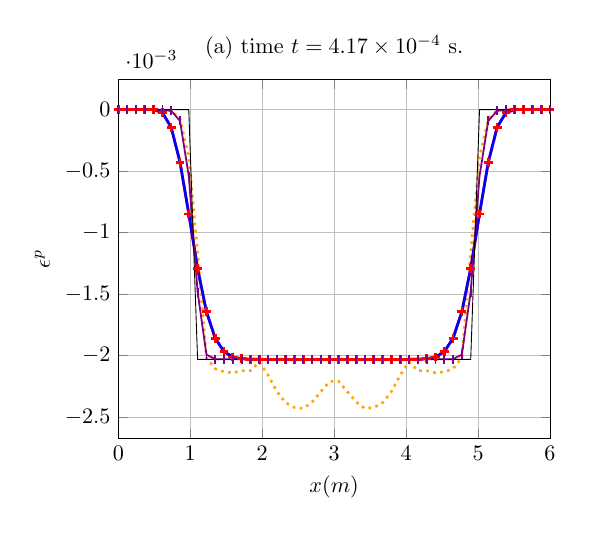
\begin{tikzpicture}[scale=0.8]
\begin{axis}[xlabel=$x (m)$,ylabel=$\epsilon^p$,ymajorgrids=true,xmajorgrids=true,legend pos=outer north east,title={(a) time $t = 4.17\times 10^{-4} $ s.},xmin=0.,xmax=6.]
\addplot[Red,very thick,mark=+,solid] coordinates {(0.0,0.0) (0.12244897959183673,0.0) (0.24489795918367346,0.0) (0.36734693877551017,0.0) (0.4897959183673469,0.0) (0.6122448979591837,-2.4267855226065594e-05) (0.7346938775510203,-0.00014452073597361284) (0.8571428571428571,-0.0004275642401009131) (0.9795918367346939,-0.0008483282066457896) (1.1020408163265305,-0.0012913872123487611) (1.2244897959183674,-0.001642660920094959) (1.346938775510204,-0.0018602413103573651) (1.4693877551020407,-0.0019680574666657586) (1.5918367346938775,-0.00201146561977191) (1.7142857142857142,-0.002025805454394895) (1.836734693877551,-0.0020297136017104972) (1.9591836734693877,-0.002030593864489664) (2.0816326530612246,-0.002030757436013639) (2.204081632653061,-0.0020307823755532774) (2.326530612244898,-0.002030785465084119) (2.4489795918367347,-0.0020307857712710334) (2.571428571428571,-0.00203078579497771) (2.693877551020408,-0.0020307857963597366) (2.816326530612245,-0.002030785796416807) (2.9387755102040813,-0.002030785796418294) (3.061224489795918,-0.002030785796418294) (3.183673469387755,-0.0020307857964168056) (3.306122448979592,-0.002030785796359739) (3.4285714285714284,-0.0020307857949777124) (3.5510204081632653,-0.002030785771271032) (3.673469387755102,-0.002030785465084119) (3.7959183673469385,-0.002030782375553277) (3.9183673469387754,-0.0020307574360136386) (4.040816326530612,-0.002030593864489664) (4.163265306122449,-0.0020297136017104964) (4.285714285714286,-0.0020258054543948927) (4.408163265306122,-0.002011465619771909) (4.530612244897959,-0.0019680574666657573) (4.653061224489796,-0.0018602413103573651) (4.775510204081632,-0.0016426609200949592) (4.8979591836734695,-0.001291387212348762) (5.020408163265306,-0.0008483282066457893) (5.142857142857142,-0.00042756424010091193) (5.26530612244898,-0.00014452073597361384) (5.387755102040816,-2.4267855226067292e-05) (5.5102040816326525,0.0) (5.63265306122449,0.0) (5.755102040816326,0.0) (5.877551020408163,0.0) (6.0,0.0) };
\addplot[Orange,very thick,mark=none,dotted] coordinates {(0.0011999999999999927,0.0) (0.12359999999999997,0.0) (0.24599999999999994,0.0) (0.36839999999999995,0.0) (0.4907999999999999,0.0) (0.6131999999999999,-3.6185144371068533e-07) (0.7355999999999999,-8.019549939201378e-06) (0.858,-7.545863055389513e-05) (0.9803999999999998,-0.00038823448768833166) (1.1027999999999998,-0.0011649510446652884) (1.2251999999999996,-0.0020167797859788647) (1.3475999999999997,-0.002107399619958115) (1.4699999999999998,-0.002131770374563102) (1.5923999999999996,-0.0021403574192086572) (1.7147999999999997,-0.0021224712498380525) (1.8371999999999995,-0.0021223153729543927) (1.9595999999999996,-0.002051517588290279) (2.0819999999999994,-0.00215869886386764) (2.2043999999999997,-0.00229323761080671) (2.3267999999999995,-0.002383730340592019) (2.4491999999999994,-0.002422023782426279) (2.5715999999999997,-0.0024301527006305407) (2.6939999999999995,-0.0023776240406298606) (2.8163999999999993,-0.0022924966391795762) (2.9387999999999996,-0.002209718054457858) (3.0611999999999995,-0.002209718054457853) (3.1835999999999993,-0.00229249663917957) (3.305999999999999,-0.002377624040629834) (3.4283999999999994,-0.0024301527006305133) (3.5507999999999993,-0.0024220237824262893) (3.673199999999999,-0.0023837303405920274) (3.7955999999999994,-0.0022932376108067225) (3.9179999999999993,-0.002158698863867652) (4.040399999999999,-0.0020515175882902612) (4.1628,-0.00212231537295439) (4.2852,-0.002122471249838043) (4.4076,-0.002140357419208655) (4.53,-0.0021317703745630944) (4.6524,-0.0021073996199581038) (4.7748,-0.002016779785978835) (4.8972,-0.0011649510446653149) (5.0196,-0.00038823448768831226) (5.142,-7.54586305539126e-05) (5.2644,-8.019549939178096e-06) (5.3868,-3.6185144371335306e-07) (5.5092,0.0) (5.6316,0.0) (5.754,0.0) (5.8764,0.0) (5.9988,0.0) };
\addplot[Blue,very thick,mark=none,solid] coordinates {(0.0011999999999999927,0.0) (0.12359999999999997,0.0) (0.24599999999999994,0.0) (0.36839999999999995,0.0) (0.4907999999999999,0.0) (0.6131999999999999,-2.4267855226066533e-05) (0.7355999999999999,-0.00014452073597361162) (0.858,-0.0004275642401009113) (0.9803999999999998,-0.0008483282066457879) (1.1027999999999998,-0.0012913872123487594) (1.2251999999999996,-0.0016426609200949575) (1.3475999999999997,-0.0018602413103573636) (1.4699999999999998,-0.0019680574666657573) (1.5923999999999996,-0.002011465619771908) (1.7147999999999997,-0.002025805454394894) (1.8371999999999995,-0.0020297136017104955) (1.9595999999999996,-0.0020305938644896646) (2.0819999999999994,-0.002030757436013637) (2.2043999999999997,-0.002030782375553278) (2.3267999999999995,-0.002030785465084118) (2.4491999999999994,-0.0020307857712710316) (2.5715999999999997,-0.002030785794977712) (2.6939999999999995,-0.002030785796359737) (2.8163999999999993,-0.002030785796416805) (2.9387999999999996,-0.0020307857964182922) (3.0611999999999995,-0.0020307857964182935) (3.1835999999999993,-0.002030785796416805) (3.305999999999999,-0.002030785796359737) (3.4283999999999994,-0.002030785794977712) (3.5507999999999993,-0.0020307857712710316) (3.673199999999999,-0.0020307854650841186) (3.7955999999999994,-0.002030782375553278) (3.9179999999999993,-0.002030757436013637) (4.040399999999999,-0.0020305938644896646) (4.1628,-0.0020297136017104955) (4.2852,-0.002025805454394893) (4.4076,-0.002011465619771907) (4.53,-0.0019680574666657573) (4.6524,-0.0018602413103573636) (4.7748,-0.0016426609200949566) (4.8972,-0.0012913872123487594) (5.0196,-0.0008483282066457876) (5.142,-0.0004275642401009109) (5.2644,-0.00014452073597361162) (5.3868,-2.4267855226066533e-05) (5.5092,0.0) (5.6316,0.0) (5.754,0.0) (5.8764,0.0) (5.9988,0.0) };
\addplot[Purple,thick,mark=|,solid] coordinates {(0.0011999999999999927,0.0) (0.12359999999999997,0.0) (0.24599999999999994,0.0) (0.36839999999999995,0.0) (0.4907999999999999,0.0) (0.6131999999999999,-5.394021759754931e-07) (0.7355999999999999,-1.010771354391672e-05) (0.858,-9.168096769918878e-05) (0.9803999999999998,-0.0005435535234499527) (1.1027999999999998,-0.0014841083655069223) (1.2251999999999996,-0.001991887176242578) (1.3475999999999997,-0.002028854598935097) (1.4699999999999998,-0.0020307027185062754) (1.5923999999999996,-0.002030782602337539) (1.7147999999999997,-0.0020307856903745234) (1.8371999999999995,-0.002030785793411752) (1.9595999999999996,-0.002030785796346042) (2.0819999999999994,-0.002030785796416862) (2.2043999999999997,-0.002030785796418289) (2.3267999999999995,-0.0020307857964183135) (2.4491999999999994,-0.0020307857964183135) (2.5715999999999997,-0.0020307857964183135) (2.6939999999999995,-0.0020307857964183135) (2.8163999999999993,-0.0020307857964183135) (2.9387999999999996,-0.0020307857964183135) (3.0611999999999995,-0.0020307857964183135) (3.1835999999999993,-0.0020307857964183135) (3.305999999999999,-0.0020307857964183126) (3.4283999999999994,-0.0020307857964183135) (3.5507999999999993,-0.0020307857964183126) (3.673199999999999,-0.0020307857964183126) (3.7955999999999994,-0.002030785796418291) (3.9179999999999993,-0.0020307857964168632) (4.040399999999999,-0.0020307857963460427) (4.1628,-0.0020307857934117523) (4.2852,-0.002030785690374525) (4.4076,-0.0020307826023375384) (4.53,-0.0020307027185062733) (4.6524,-0.002028854598935106) (4.7748,-0.0019918871762425686) (4.8972,-0.0014841083655069208) (5.0196,-0.0005435535234499549) (5.142,-9.168096769918878e-05) (5.2644,-1.010771354391672e-05) (5.3868,-5.394021759754931e-07) (5.5092,0.0) (5.6316,0.0) (5.754,0.0) (5.8764,0.0) (5.9988,0.0) };
\addplot[black,thin,mark=none,solid] coordinates {(0.0,-0.0) (0.12244897959183673,-0.0) (0.24489795918367346,-0.0) (0.36734693877551017,-0.0) (0.4897959183673469,-0.0) (0.6122448979591837,-0.0) (0.7346938775510203,-0.0) (0.8571428571428571,-0.0) (0.9795918367346939,-0.0) (1.1020408163265305,-0.002030785796418313) (1.2244897959183674,-0.002030785796418313) (1.346938775510204,-0.002030785796418313) (1.4693877551020407,-0.002030785796418313) (1.5918367346938775,-0.002030785796418313) (1.7142857142857142,-0.002030785796418313) (1.836734693877551,-0.002030785796418313) (1.9591836734693877,-0.002030785796418313) (2.0816326530612246,-0.002030785796418313) (2.204081632653061,-0.002030785796418313) (2.326530612244898,-0.002030785796418313) (2.4489795918367347,-0.002030785796418313) (2.571428571428571,-0.002030785796418313) (2.693877551020408,-0.002030785796418313) (2.816326530612245,-0.002030785796418313) (2.9387755102040813,-0.002030785796418313) (3.061224489795918,-0.002030785796418313) (3.183673469387755,-0.002030785796418313) (3.306122448979592,-0.002030785796418313) (3.4285714285714284,-0.002030785796418313) (3.5510204081632653,-0.002030785796418313) (3.673469387755102,-0.002030785796418313) (3.7959183673469385,-0.002030785796418313) (3.9183673469387754,-0.002030785796418313) (4.040816326530612,-0.002030785796418313) (4.163265306122449,-0.002030785796418313) (4.285714285714286,-0.002030785796418313) (4.408163265306122,-0.002030785796418313) (4.530612244897959,-0.002030785796418313) (4.653061224489796,-0.002030785796418313) (4.775510204081632,-0.002030785796418313) (4.8979591836734695,-0.002030785796418313) (5.020408163265306,-0.0) (5.142857142857142,-0.0) (5.26530612244898,-0.0) (5.387755102040816,-0.0) (5.5102040816326525,-0.0) (5.63265306122449,-0.0) (5.755102040816326,-0.0) (5.877551020408163,-0.0) (6.0,-0.0) };
%\legend{dgmpm,fem,fvm,fvm (SB),exact}
\end{axis}
\end{tikzpicture}
%%% Local Variables:
%%% mode: latex
%%% TeX-master: "../../mainManuscript"
%%% End:
}
%   {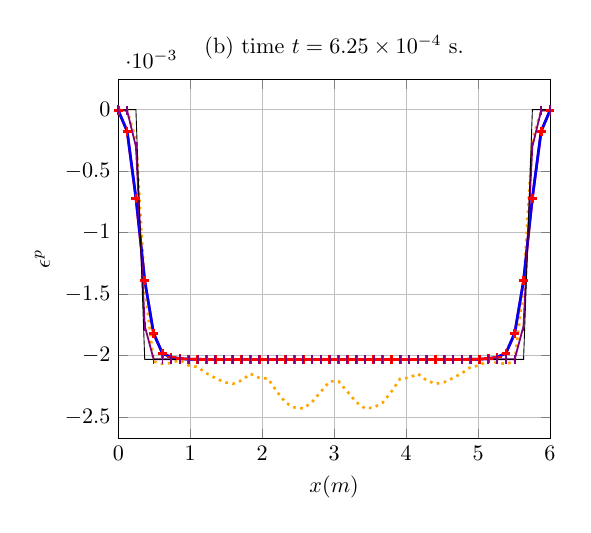
\begin{tikzpicture}[scale=0.8]
\begin{axis}[xlabel=$x (m)$,ylabel=$\epsilon^p$,ymajorgrids=true,xmajorgrids=true,legend pos=outer north east,title={(b) time $t = 6.25\times 10^{-4} $ s.},xmin=0.,xmax=6.]
\addplot[Red,very thick,mark=+,solid] coordinates {(0.0,-8.02367288935203e-06) (0.12244897959183673,-0.00017614426387335805) (0.24489795918367346,-0.0007207542691858686) (0.36734693877551017,-0.0013919930410856215) (0.4897959183673469,-0.001818355598439618) (0.6122448979591837,-0.001981300761387861) (0.7346938775510203,-0.0020125975551096974) (0.8571428571428571,-0.002024874952136019) (0.9795918367346939,-0.0020290867696967987) (1.1020408163265305,-0.002030353909504423) (1.2244897959183674,-0.0020306887880741907) (1.346938775510204,-0.0020307665725143873) (1.4693877551020407,-0.0020307824435747243) (1.5918367346938775,-0.0020307852835259937) (1.7142857142857142,-0.0020307857279245408) (1.836734693877551,-0.0020307857884822454) (1.9591836734693877,-0.00203078579562695) (2.0816326530612246,-0.002030785796351117) (2.204081632653061,-0.0020307857964135248) (2.326530612244898,-0.002030785796418031) (2.4489795918367347,-0.002030785796418302) (2.571428571428571,-0.0020307857964183135) (2.693877551020408,-0.002030785796418313) (2.816326530612245,-0.002030785796418313) (2.9387755102040813,-0.002030785796418314) (3.061224489795918,-0.0020307857964183135) (3.183673469387755,-0.0020307857964183135) (3.306122448979592,-0.0020307857964183126) (3.4285714285714284,-0.0020307857964183113) (3.5510204081632653,-0.0020307857964183005) (3.673469387755102,-0.002030785796418031) (3.7959183673469385,-0.0020307857964135217) (3.9183673469387754,-0.0020307857963511138) (4.040816326530612,-0.002030785795626948) (4.163265306122449,-0.0020307857884822433) (4.285714285714286,-0.0020307857279245403) (4.408163265306122,-0.0020307852835259915) (4.530612244897959,-0.0020307824435747226) (4.653061224489796,-0.0020307665725143842) (4.775510204081632,-0.002030688788074188) (4.8979591836734695,-0.0020303539095044196) (5.020408163265306,-0.0020290867696967953) (5.142857142857142,-0.0020248749521360144) (5.26530612244898,-0.0020125975551096966) (5.387755102040816,-0.0019813007613878565) (5.5102040816326525,-0.0018183555984396154) (5.63265306122449,-0.0013919930410856195) (5.755102040816326,-0.0007207542691858678) (5.877551020408163,-0.0001761442638733595) (6.0,-8.023672889353243e-06) };
\addplot[Orange,very thick,mark=none,dotted] coordinates {(0.0011999999999999927,-3.955614396475477e-08) (0.12359999999999997,-9.316948262183543e-06) (0.24599999999999994,-0.00024388789370993148) (0.36839999999999995,-0.001442592108388968) (0.4907999999999999,-0.00204828198640817) (0.6131999999999999,-0.002067557310378223) (0.7355999999999999,-0.0020594157964176534) (0.858,-0.0020372674628823476) (0.9803999999999998,-0.0020807928937422093) (1.1027999999999998,-0.0020931249622338447) (1.2251999999999996,-0.0021438341556582357) (1.3475999999999997,-0.0021820311184349702) (1.4699999999999998,-0.002216170966229309) (1.5923999999999996,-0.002229918265686059) (1.7147999999999997,-0.002201581328157663) (1.8371999999999995,-0.0021483028099073733) (1.9595999999999996,-0.002180462898277691) (2.0819999999999994,-0.0021876731020669623) (2.2043999999999997,-0.00229323761080671) (2.3267999999999995,-0.002383730340592019) (2.4491999999999994,-0.002422023782426279) (2.5715999999999997,-0.0024301527006305407) (2.6939999999999995,-0.0023776240406298606) (2.8163999999999993,-0.0022924966391795762) (2.9387999999999996,-0.002209718054457858) (3.0611999999999995,-0.002209718054457853) (3.1835999999999993,-0.00229249663917957) (3.305999999999999,-0.002377624040629834) (3.4283999999999994,-0.0024301527006305133) (3.5507999999999993,-0.0024220237824262893) (3.673199999999999,-0.0023837303405920274) (3.7955999999999994,-0.0022932376108067225) (3.9179999999999993,-0.002187673102066998) (4.040399999999999,-0.0021804628982777176) (4.1628,-0.002148302809907372) (4.2852,-0.00220158132815765) (4.4076,-0.0022299182656860483) (4.53,-0.0022161709662292563) (4.6524,-0.0021820311184349156) (4.7748,-0.002143834155658191) (4.8972,-0.0020931249622338105) (5.0196,-0.002080792893742207) (5.142,-0.002037267462882373) (5.2644,-0.002059415796417687) (5.3868,-0.0020675573103782394) (5.5092,-0.0020482819864081916) (5.6316,-0.0014425921083889624) (5.754,-0.00024388789370993877) (5.8764,-9.316948262168749e-06) (5.9988,-3.955614396669495e-08) };
\addplot[Blue,very thick,mark=none,solid] coordinates {(0.0011999999999999927,-8.023672889352762e-06) (0.12359999999999997,-0.00017614426387335818) (0.24599999999999994,-0.0007207542691858663) (0.36839999999999995,-0.0013919930410856193) (0.4907999999999999,-0.0018183555984396156) (0.6131999999999999,-0.0019813007613878556) (0.7355999999999999,-0.0020125975551096944) (0.858,-0.0020248749521360153) (0.9803999999999998,-0.002029086769696795) (1.1027999999999998,-0.0020303539095044188) (1.2251999999999996,-0.0020306887880741876) (1.3475999999999997,-0.0020307665725143834) (1.4699999999999998,-0.0020307824435747226) (1.5923999999999996,-0.0020307852835259902) (1.7147999999999997,-0.002030785727924537) (1.8371999999999995,-0.002030785788482242) (1.9595999999999996,-0.002030785795626947) (2.0819999999999994,-0.002030785796351112) (2.2043999999999997,-0.0020307857964135196) (2.3267999999999995,-0.002030785796418031) (2.4491999999999994,-0.0020307857964183005) (2.5715999999999997,-0.0020307857964183126) (2.6939999999999995,-0.0020307857964183143) (2.8163999999999993,-0.0020307857964183143) (2.9387999999999996,-0.0020307857964183143) (3.0611999999999995,-0.0020307857964183135) (3.1835999999999993,-0.0020307857964183135) (3.305999999999999,-0.0020307857964183135) (3.4283999999999994,-0.0020307857964183135) (3.5507999999999993,-0.0020307857964183005) (3.673199999999999,-0.0020307857964180303) (3.7955999999999994,-0.002030785796413521) (3.9179999999999993,-0.0020307857963511138) (4.040399999999999,-0.002030785795626947) (4.1628,-0.002030785788482243) (4.2852,-0.0020307857279245373) (4.4076,-0.0020307852835259902) (4.53,-0.0020307824435747213) (4.6524,-0.0020307665725143834) (4.7748,-0.0020306887880741867) (4.8972,-0.0020303539095044188) (5.0196,-0.002029086769696795) (5.142,-0.0020248749521360153) (5.2644,-0.0020125975551096944) (5.3868,-0.001981300761387855) (5.5092,-0.001818355598439614) (5.6316,-0.0013919930410856186) (5.754,-0.0007207542691858663) (5.8764,-0.0001761442638733578) (5.9988,-8.023672889352762e-06) };
\addplot[Purple,thick,mark=|,solid] coordinates {(0.0011999999999999927,-5.896527565960431e-08) (0.12359999999999997,-1.0175215434139024e-05) (0.24599999999999994,-0.00030290594091646547) (0.36839999999999995,-0.0017602606272338914) (0.4907999999999999,-0.002029328897607904) (0.6131999999999999,-0.0020307790770812324) (0.7355999999999999,-0.0020307854952318397) (0.858,-0.00203078578407098) (0.9803999999999998,-0.0020307857959587752) (1.1027999999999998,-0.002030785796402892) (1.2251999999999996,-0.002030785796417849) (1.3475999999999997,-0.0020307857964183013) (1.4699999999999998,-0.0020307857964183135) (1.5923999999999996,-0.0020307857964183126) (1.7147999999999997,-0.0020307857964183135) (1.8371999999999995,-0.0020307857964183135) (1.9595999999999996,-0.0020307857964183135) (2.0819999999999994,-0.0020307857964183126) (2.2043999999999997,-0.0020307857964183135) (2.3267999999999995,-0.0020307857964183135) (2.4491999999999994,-0.0020307857964183135) (2.5715999999999997,-0.0020307857964183135) (2.6939999999999995,-0.0020307857964183135) (2.8163999999999993,-0.0020307857964183135) (2.9387999999999996,-0.0020307857964183135) (3.0611999999999995,-0.0020307857964183135) (3.1835999999999993,-0.0020307857964183135) (3.305999999999999,-0.0020307857964183135) (3.4283999999999994,-0.0020307857964183135) (3.5507999999999993,-0.0020307857964183135) (3.673199999999999,-0.0020307857964183135) (3.7955999999999994,-0.0020307857964183126) (3.9179999999999993,-0.0020307857964183135) (4.040399999999999,-0.0020307857964183135) (4.1628,-0.0020307857964183126) (4.2852,-0.0020307857964183117) (4.4076,-0.0020307857964183117) (4.53,-0.0020307857964183117) (4.6524,-0.0020307857964182996) (4.7748,-0.0020307857964178473) (4.8972,-0.002030785796402895) (5.0196,-0.002030785795958776) (5.142,-0.002030785784070983) (5.2644,-0.002030785495231843) (5.3868,-0.0020307790770812315) (5.5092,-0.0020293288976078977) (5.6316,-0.0017602606272338914) (5.754,-0.0003029059409164685) (5.8764,-1.0175215434139024e-05) (5.9988,-5.896527565960431e-08) };
\addplot[black,thin,mark=none,solid] coordinates {(0.0,-0.0) (0.12244897959183673,-0.0) (0.24489795918367346,-0.0) (0.36734693877551017,-0.002030785796418313) (0.4897959183673469,-0.002030785796418313) (0.6122448979591837,-0.002030785796418313) (0.7346938775510203,-0.002030785796418313) (0.8571428571428571,-0.002030785796418313) (0.9795918367346939,-0.002030785796418313) (1.1020408163265305,-0.002030785796418313) (1.2244897959183674,-0.002030785796418313) (1.346938775510204,-0.002030785796418313) (1.4693877551020407,-0.002030785796418313) (1.5918367346938775,-0.002030785796418313) (1.7142857142857142,-0.002030785796418313) (1.836734693877551,-0.002030785796418313) (1.9591836734693877,-0.002030785796418313) (2.0816326530612246,-0.002030785796418313) (2.204081632653061,-0.002030785796418313) (2.326530612244898,-0.002030785796418313) (2.4489795918367347,-0.002030785796418313) (2.571428571428571,-0.002030785796418313) (2.693877551020408,-0.002030785796418313) (2.816326530612245,-0.002030785796418313) (2.9387755102040813,-0.002030785796418313) (3.061224489795918,-0.002030785796418313) (3.183673469387755,-0.002030785796418313) (3.306122448979592,-0.002030785796418313) (3.4285714285714284,-0.002030785796418313) (3.5510204081632653,-0.002030785796418313) (3.673469387755102,-0.002030785796418313) (3.7959183673469385,-0.002030785796418313) (3.9183673469387754,-0.002030785796418313) (4.040816326530612,-0.002030785796418313) (4.163265306122449,-0.002030785796418313) (4.285714285714286,-0.002030785796418313) (4.408163265306122,-0.002030785796418313) (4.530612244897959,-0.002030785796418313) (4.653061224489796,-0.002030785796418313) (4.775510204081632,-0.002030785796418313) (4.8979591836734695,-0.002030785796418313) (5.020408163265306,-0.002030785796418313) (5.142857142857142,-0.002030785796418313) (5.26530612244898,-0.002030785796418313) (5.387755102040816,-0.002030785796418313) (5.5102040816326525,-0.002030785796418313) (5.63265306122449,-0.002030785796418313) (5.755102040816326,-0.0) (5.877551020408163,-0.0) (6.0,-0.0) };
%\legend{dgmpm,fem,fvm,fvm (SB),exact}
\end{axis}
\end{tikzpicture}
%%% Local Variables:
%%% mode: latex
%%% TeX-master: "../../mainManuscript"
%%% End:
}
%   {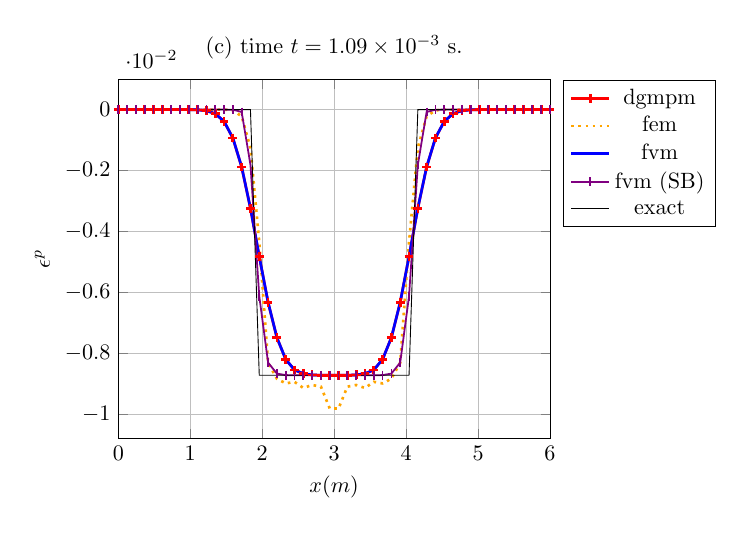
\begin{tikzpicture}[scale=0.8]
\begin{axis}[xlabel=$x (m)$,ylabel=$\epsilon^p$,ymajorgrids=true,xmajorgrids=true,legend pos=outer north east,title={(c) time $t = 1.09\times 10^{-3} $ s.},xmin=0.,xmax=6.]
\addplot[Red,very thick,mark=+,solid] coordinates {(0.0,-5.676632835751488e-19) (0.12244897959183673,-2.3898624238513766e-16) (0.24489795918367346,-3.735990751357306e-14) (0.36734693877551017,-2.3089144911084856e-12) (0.4897959183673469,-7.596762237094698e-11) (0.6122448979591837,-1.5415975357804979e-09) (0.7346938775510203,-2.1087029002110162e-08) (0.8571428571428571,-2.0628580472526095e-07) (0.9795918367346939,-1.5051975779320511e-06) (1.1020408163265305,-8.452232526292688e-06) (1.2244897959183674,-3.741900938747327e-05) (1.346938775510204,-0.00013315210803806102) (1.4693877551020407,-0.00038701776930482674) (1.5918367346938775,-0.0009319386970470464) (1.7142857142857142,-0.0018842066770200564) (1.836734693877551,-0.0032431409441831516) (1.9591836734693877,-0.004827293901207316) (2.0816326530612246,-0.00633202118341673) (2.204081632653061,-0.007489880430691718) (2.326530612244898,-0.008204526972019307) (2.4489795918367347,-0.008552921390073501) (2.571428571428571,-0.008674876019514461) (2.693877551020408,-0.008716486656783273) (2.816326530612245,-0.008726887116624966) (2.9387755102040813,-0.008728580772745199) (3.061224489795918,-0.008728580772745199) (3.183673469387755,-0.008726887116624966) (3.306122448979592,-0.00871648665678328) (3.4285714285714284,-0.008674876019514466) (3.5510204081632653,-0.008552921390073511) (3.673469387755102,-0.008204526972019318) (3.7959183673469385,-0.007489880430691721) (3.9183673469387754,-0.00633202118341673) (4.040816326530612,-0.0048272939012073204) (4.163265306122449,-0.0032431409441831525) (4.285714285714286,-0.001884206677020053) (4.408163265306122,-0.0009319386970470392) (4.530612244897959,-0.0003870177693048181) (4.653061224489796,-0.0001331521080380519) (4.775510204081632,-3.7419009387462476e-05) (4.8979591836734695,-8.452232526284741e-06) (5.020408163265306,-1.5051975779246716e-06) (5.142857142857142,-2.0628580471617835e-07) (5.26530612244898,-2.1087028991608393e-08) (5.387755102040816,-1.5415975312391917e-09) (5.5102040816326525,-7.596762123562041e-11) (5.63265306122449,-2.308913923445202e-12) (5.755102040816326,-3.7358772187005907e-14) (5.877551020408163,-2.4097306387765065e-16) (6.0,-8.514949253627233e-19) };
\addplot[Orange,very thick,mark=none,dotted] coordinates {(0.0011999999999999927,0.0) (0.12359999999999997,0.0) (0.24599999999999994,0.0) (0.36839999999999995,0.0) (0.4907999999999999,-2.7815500895182294e-17) (0.6131999999999999,-3.8601103283110115e-17) (0.7355999999999999,-2.0038513910202753e-16) (0.858,-1.7291875112624395e-14) (0.9803999999999998,-1.4890633878253755e-12) (1.1027999999999998,-8.711066870462328e-11) (1.2251999999999996,-3.5097774352346146e-09) (1.3475999999999997,-9.795044328882581e-08) (1.4699999999999998,-1.8896649221051307e-06) (1.5923999999999996,-2.4938869347233433e-05) (1.7147999999999997,-0.00022044973282056137) (1.8371999999999995,-0.0012586085323126788) (1.9595999999999996,-0.004366206064980092) (2.0819999999999994,-0.008315998828072487) (2.2043999999999997,-0.008841830788122323) (2.3267999999999995,-0.008995195469072521) (2.4491999999999994,-0.008944386605810638) (2.5715999999999997,-0.009146349400835571) (2.6939999999999995,-0.00904766889023616) (2.8163999999999993,-0.00910247337367582) (2.9387999999999996,-0.009819714666194801) (3.0611999999999995,-0.0098197146661948) (3.1835999999999993,-0.009102473373675955) (3.305999999999999,-0.009047668890236175) (3.4283999999999994,-0.009146349400835545) (3.5507999999999993,-0.008944386605810636) (3.673199999999999,-0.008995195469072475) (3.7955999999999994,-0.00884183078812235) (3.9179999999999993,-0.008315998828072471) (4.040399999999999,-0.004366206064980109) (4.1628,-0.0012586085323127117) (4.2852,-0.00022044973282050575) (4.4076,-2.4938869347250462e-05) (4.53,-1.8896649221051307e-06) (4.6524,-9.795044333225205e-08) (4.7748,-3.5097774522645135e-09) (4.8972,-8.711060172035581e-11) (5.0196,-1.4891476858229865e-12) (5.142,-1.7265194938296362e-14) (5.2644,-1.9045103163946243e-16) (5.3868,-1.7029898507254465e-18) (5.5092,-1.5043077014741444e-17) (5.6316,-1.7029898507254465e-18) (5.754,-1.4759245372953867e-17) (5.8764,-1.7029898507254465e-18) (5.9988,0.0) };
\addplot[Blue,very thick,mark=none,solid] coordinates {(0.0011999999999999927,0.0) (0.12359999999999997,-2.384185791015625e-16) (0.24599999999999994,-3.736019134521484e-14) (0.36839999999999995,-2.3089170455932617e-12) (0.4907999999999999,-7.596761584281921e-11) (0.6131999999999999,-1.5415975272655486e-09) (0.7355999999999999,-2.1087028992176057e-08) (0.858,-2.0628580471873284e-07) (0.9803999999999998,-1.5051975779294967e-06) (1.1027999999999998,-8.452232526284456e-06) (1.2251999999999996,-3.741900938746333e-05) (1.3475999999999997,-0.00013315210803804993) (1.4699999999999998,-0.00038701776930482386) (1.5923999999999996,-0.0009319386970470428) (1.7147999999999997,-0.001884206677020061) (1.8371999999999995,-0.003243140944183153) (1.9595999999999996,-0.004827293901207322) (2.0819999999999994,-0.006332021183416736) (2.2043999999999997,-0.007489880430691725) (2.3267999999999995,-0.008204526972019321) (2.4491999999999994,-0.008552921390073513) (2.5715999999999997,-0.008674876019514464) (2.6939999999999995,-0.008716486656783276) (2.8163999999999993,-0.008726887116624964) (2.9387999999999996,-0.008728580772745204) (3.0611999999999995,-0.008728580772745204) (3.1835999999999993,-0.008726887116624964) (3.305999999999999,-0.008716486656783276) (3.4283999999999994,-0.008674876019514464) (3.5507999999999993,-0.008552921390073513) (3.673199999999999,-0.008204526972019321) (3.7955999999999994,-0.007489880430691725) (3.9179999999999993,-0.006332021183416736) (4.040399999999999,-0.004827293901207322) (4.1628,-0.003243140944183153) (4.2852,-0.001884206677020061) (4.4076,-0.0009319386970470428) (4.53,-0.00038701776930482386) (4.6524,-0.00013315210803804993) (4.7748,-3.741900938746333e-05) (4.8972,-8.452232526284456e-06) (5.0196,-1.5051975779294967e-06) (5.142,-2.0628580471873284e-07) (5.2644,-2.1087028992176057e-08) (5.3868,-1.5415975272655486e-09) (5.5092,-7.596761584281921e-11) (5.6316,-2.3089170455932617e-12) (5.754,-3.736019134521484e-14) (5.8764,-2.384185791015625e-16) (5.9988,0.0) };
\addplot[Purple,thick,mark=|,solid] coordinates {(0.0011999999999999927,0.0) (0.12359999999999997,0.0) (0.24599999999999994,0.0) (0.36839999999999995,0.0) (0.4907999999999999,0.0) (0.6131999999999999,0.0) (0.7355999999999999,0.0) (0.858,-2.8014183044433593e-16) (0.9803999999999998,-2.1100044250488282e-14) (1.1027999999999998,-1.2365996837615966e-12) (1.2251999999999996,-5.9033864736557e-11) (1.3475999999999997,-2.3761736869812012e-09) (1.4699999999999998,-8.325840687155723e-08) (1.5923999999999996,-2.6323343349337577e-06) (1.7147999999999997,-7.853228000084162e-05) (1.8371999999999995,-0.0018212430710175336) (1.9595999999999996,-0.006137739318747551) (2.0819999999999994,-0.008311894308815801) (2.2043999999999997,-0.008672824985492957) (2.3267999999999995,-0.008722601697817814) (2.4491999999999994,-0.00872819127980076) (2.5715999999999997,-0.008728663911155045) (2.6939999999999995,-0.008728711882144921) (2.8163999999999993,-0.008728715435078365) (2.9387999999999996,-0.0087287156054703) (3.0611999999999995,-0.0087287156054703) (3.1835999999999993,-0.008728715435078365) (3.305999999999999,-0.008728711882144921) (3.4283999999999994,-0.008728663911155045) (3.5507999999999993,-0.00872819127980076) (3.673199999999999,-0.008722601697817814) (3.7955999999999994,-0.008672824985492957) (3.9179999999999993,-0.008311894308815794) (4.040399999999999,-0.006137739318747556) (4.1628,-0.0018212430710175217) (4.2852,-7.853228000084758e-05) (4.4076,-2.6323343349575996e-06) (4.53,-8.325840684175491e-08) (4.6524,-2.37617369890213e-09) (4.7748,-5.903387665748596e-11) (4.8972,-1.2365996837615966e-12) (5.0196,-2.1100044250488282e-14) (5.142,-2.8014183044433593e-16) (5.2644,0.0) (5.3868,0.0) (5.5092,0.0) (5.6316,0.0) (5.754,0.0) (5.8764,0.0) (5.9988,0.0) };
\addplot[black,thin,mark=none,solid] coordinates {(0.0,-0.0) (0.12244897959183673,-0.0) (0.24489795918367346,-0.0) (0.36734693877551017,-0.0) (0.4897959183673469,-0.0) (0.6122448979591837,-0.0) (0.7346938775510203,-0.0) (0.8571428571428571,-0.0) (0.9795918367346939,-0.0) (1.1020408163265305,-0.0) (1.2244897959183674,-0.0) (1.346938775510204,-0.0) (1.4693877551020407,-0.0) (1.5918367346938775,-0.0) (1.7142857142857142,-0.0) (1.836734693877551,-0.0) (1.9591836734693877,-0.008728715609439695) (2.0816326530612246,-0.008728715609439695) (2.204081632653061,-0.008728715609439695) (2.326530612244898,-0.008728715609439695) (2.4489795918367347,-0.008728715609439695) (2.571428571428571,-0.008728715609439695) (2.693877551020408,-0.008728715609439695) (2.816326530612245,-0.008728715609439695) (2.9387755102040813,-0.008728715609439695) (3.061224489795918,-0.008728715609439695) (3.183673469387755,-0.008728715609439695) (3.306122448979592,-0.008728715609439695) (3.4285714285714284,-0.008728715609439695) (3.5510204081632653,-0.008728715609439695) (3.673469387755102,-0.008728715609439695) (3.7959183673469385,-0.008728715609439695) (3.9183673469387754,-0.008728715609439695) (4.040816326530612,-0.008728715609439695) (4.163265306122449,-0.0) (4.285714285714286,-0.0) (4.408163265306122,-0.0) (4.530612244897959,-0.0) (4.653061224489796,-0.0) (4.775510204081632,-0.0) (4.8979591836734695,-0.0) (5.020408163265306,-0.0) (5.142857142857142,-0.0) (5.26530612244898,-0.0) (5.387755102040816,-0.0) (5.5102040816326525,-0.0) (5.63265306122449,-0.0) (5.755102040816326,-0.0) (5.877551020408163,-0.0) (6.0,-0.0) };
\legend{dgmpm,fem,fvm,fvm (SB),exact}
\end{axis}
\end{tikzpicture}
%%% Local Variables:
%%% mode: latex
%%% TeX-master: "../../mainManuscript"
%%% End:
}
%   \caption{elastic-plastic RP epsp}
%   \label{fig:epsp_elastoplastic_RP}
% \end{figure}


%%% Local Variables:
%%% mode: latex
%%% TeX-master: "../mainManuscript"
%%% End: